%Generazione delle variabili che andranno a sostituire quelle del template 'HomePage.tex'
\newcommand{\documento}{\DDP}
\newcommand{\nomedocumentofisico}{DefinizioneDiProdotto\_v3\_0\_0.pdf}
\newcommand{\redazione}{\FB\\ & \AF\\ & \GN\\ & \GR\\ & \SM\\ & \MP\\ & \MV}
\newcommand{\verifica}{\GN\\ & \SM\\ & \MV}
\newcommand{\approvazione}{\MP}
\newcommand{\uso}{Esterno}
\newcommand{\datacreazione}{23 Febbraio 2016}
\newcommand{\datamodifica}{14 Maggio 2016}
\newcommand{\stato}{Approvato}
\newcommand{\destinateTo}{\TV, \\ & \RC, \\ & \ZU}
\newcommand{\versione}{3}

\def\TABELLE{false}	%abilita - disabilita l'indice delle tabelle
\def\FIGURE{false} 	%abilita - disabilita l'indice delle figure

\documentclass[a4paper,11pt]{article}

%***IMPORTAZIONE PACKAGE***
\usepackage{ifthen}
\usepackage[italian]{babel}
\usepackage[utf8]{inputenc}
\usepackage[T1]{fontenc}
\usepackage{float}
\usepackage{chapterbib}
\usepackage{graphicx}
\usepackage[a4paper,top=2.5cm,bottom=2.5cm,left=2.5cm,right=2.5cm]{geometry}
\usepackage[colorlinks=true, urlcolor=black, citecolor=black, linkcolor=black]{hyperref}
\usepackage{booktabs}
\usepackage{fancyhdr}
\usepackage{totpages}
\usepackage{tabularx, array}
\usepackage{dcolumn}
\usepackage{epstopdf}
\usepackage{booktabs}
\usepackage{fancyhdr}
\usepackage{longtable}
\usepackage{calc}
\usepackage{datatool}
\usepackage[bottom]{footmisc}
\usepackage{listings} 
\usepackage{textcomp}
\usepackage{titlesec}
\usepackage{rotating} 
\usepackage{multirow}
\usepackage{placeins}
\usepackage{color}
\usepackage[table,usenames,dvipsnames]{xcolor}
\usepackage{hyperref}
\usepackage{makecell}
\usepackage{hyperref}


%***STILE PAGINA***
\pagestyle{fancy}
%no indentazione paragrafo
\setlength{\parindent}{0pt}

%***INTESTAZIONE***
\lhead{\Large{\progetto} \\ \footnotesize{\documento}}
\rhead{
\includegraphics[keepaspectratio = true, width = 25px] {../../Template/icone/LogoGruppo.png}}
\renewcommand{\headrulewidth}{0.4pt}  %Linea sotto l'intestazione

%***PIÈ DI PAGINA***
\lfoot{\textit{\gruppoLink}\\ \footnotesize{\email}}
\rfoot{\thepage} %per le prime pagine: mostra solo il numero romano
\cfoot{}
\renewcommand{\footrulewidth}{0.4pt}   %Linea sopra il piè di pagina

%***INSERIMENTO DI NUOVE SOTTOSEZIONI
\setcounter{secnumdepth}{7}		% mostra nel documento fino al livello 8 (1.2.3.4.5.6.7.8)
\setcounter{tocdepth}{7}			% mostra nell'indice fino al livello 8 (1.2.3.4.5.6.7.8)

%***LA SOTTOSEZIONE PARAGRAPH VIENE VISUALIZZATA COME UNA SECTION
\titleformat{\paragraph}{\normalfont\normalsize\bfseries}{\theparagraph}{1em}{}
\titlespacing*{\paragraph}{0pt}{3.25ex plus 1ex minus .2ex}{1.5ex plus .2ex}

\titleformat{\subparagraph}{\normalfont\normalsize\bfseries}{\thesubparagraph}{1em}{}
\titlespacing*{\subparagraph}{0pt}{3.25ex plus 1ex minus .2ex}{1.5ex plus .2ex}

\makeatletter
\newcounter{subsubparagraph}[subparagraph]
\renewcommand\thesubsubparagraph{%
  \thesubparagraph.\@arabic\c@subsubparagraph}
\newcommand\subsubparagraph{%
  \@startsection{subsubparagraph}    % counter
    {6}                              % level
    {\parindent}                     % indent
    {3.25ex \@plus 1ex \@minus .2ex} % beforeskip
    {0.75em}                           % afterskip
    {\normalfont\normalsize\bfseries}}
\newcommand\l@subsubparagraph{\@dottedtocline{6}{10em}{5.5em}} %gestione dell'indice
\newcommand{\subsubparagraphmark}[1]{}
\makeatother

\makeatletter
\newcounter{subsubsubparagraph}[subsubparagraph]
\renewcommand\thesubsubsubparagraph{%
  \thesubsubparagraph.\@arabic\c@subsubsubparagraph}
\newcommand\subsubsubparagraph{%
  \@startsection{subsubsubparagraph}    % counter
    {7}                              % level
    {\parindent}                     % indent
    {3.25ex \@plus 1ex \@minus .2ex} % beforeskip
    {0.75em}                           % afterskip
    {\normalfont\normalsize\bfseries}}
\newcommand\l@subsubsubparagraph{\@dottedtocline{7}{10em}{6.5em}} %gestione dell'indice
\newcommand{\subsubsubparagraphmark}[1]{}
\makeatother
%Generali
\newcommand{\progetto}{QuizziPedia}
\newcommand{\gruppo}{TheFellowshipOfTheCode}
\newcommand{\gruppoLink}{\href{http://thefellowshipofthecode.github.io/}{TheFellowshipOfTheCode}}
\newcommand{\email}{\href{mailto:thefellowshipofthecode@gmail.com}{thefellowshipofthecode@gmail.com}}

%Documenti
\newcommand{\AdR}{Analisi dei Requisiti}
\newcommand{\NdP}{Norme di Progetto}
\newcommand{\PdP}{Piano di Progetto}
\newcommand{\SdF}{Studio di Fattibilità}
\newcommand{\PdQ}{Piano di Qualifica}
\newcommand{\VI}{Verbale Interno}
\newcommand{\VE}{Verbale Esterno}
\newcommand{\ST}{Specifica Tecnica}
\newcommand{\DDP}{Definizione di Prodotto}
\newcommand{\MU}{Manuale Utente}
\newcommand{\G}{Glossario}
\newcommand{\LdP}{Lettera di Presentazione}
\newcommand{\NdPv}{NormeDiProgetto\_v\_1\_0\_0}
\newcommand{\PdPv}{PianoDiProgetto\_v\_1\_0\_0}
\newcommand{\PdQv}{PianoDiQualifica\_v\_1\_0\_0}
\newcommand{\SdFv}{StudioDiFattibilità\_v\_1\_0\_0}

%Componenti del gruppo
\newcommand{\AF}{Alberto Ferrara}
\newcommand{\SM}{Simone Magagna}
\newcommand{\FB}{Franco Berton}
\newcommand{\MP}{Marco Prelaz}
\newcommand{\MV}{Mattia Varotto}
\newcommand{\GN}{Matteo Gnoato}
\newcommand{\GR}{Matteo Granzotto}

%Ruoli
\newcommand{\RdP}{Responsabile di Progetto}
\newcommand{\Res}{Responsabile}
\newcommand{\Amm}{Amministratore}
\newcommand{\Ver}{Verificatore}
\newcommand{\Prog}{Progettista}
\newcommand{\Progr}{Programmatore}
\newcommand{\Ana}{Analista}
\newcommand{\RdPs}{Responsabili di Progetto}
\newcommand{\Ress}{Responsabile}
\newcommand{\Amms}{Amministratori}
\newcommand{\Vers}{Verificatori}
\newcommand{\Progs}{Progettisti}
\newcommand{\Progrs}{Programmatori}
\newcommand{\Anas}{Analisti}

%Professori e proponente
\newcommand{\TV}{Prof. Tullio Vardanega}
\newcommand{\RC}{Prof. Riccardo Cardin}
\newcommand{\ZU}{Zucchetti S.P.A.}
\newcommand{\proponente}{Zucchetti S.P.A.}

\newcommand{\diaryEntry}[5]{#2 & \emph{#4} & #3 & #5 & #1\\ \hline}

%comando per una nuova riga nella tabella del diario delle modifiche
\newcommand{\specialcell}[2][c]{%
	\begin{tabular}[#1]{@{}c@{}}#2\end{tabular}}

\renewcommand*\sectionmark[1]{\markboth{#1}{}}
\renewcommand*\subsectionmark[1]{\markright{#1}}

%Pediodi di lavoro 
\newcommand{\AR}{Analisi dei Requisiti}
\newcommand{\AD}{Analisi dei Requisiti in Dettaglio}
\newcommand{\PA}{Progettazione Architetturale}
\newcommand{\PD}{Progettazione di Dettaglio}
\newcommand{\CO}{Codifica}
\newcommand{\VV}{Verifica e Validazione}

% Revisioni
\newcommand{\RR}{Revisione dei Requisiti}
\newcommand{\RP}{Revisione di Progettazione}
\newcommand{\RQ}{Revisione di Qualifica}
\newcommand{\RA}{Revisione di Accettazione}

% Comandi analisi dei requisiti
\newcommand{\uau}{utente autenticato}
\newcommand{\uaus}{utenti autenticati}
\newcommand{\uaupro}{utente autenticato pro}
\newcommand{\uauspro}{utenti autenticati pro}

\newcommand{\myincludegraphics}[2][]{%
	\setbox0=\hbox{\phantom{X}}%
	\vtop{
		\hbox{\phantom{X}}
		\vskip-\ht0
		\hbox{\includegraphics[#1]{#2}}}}


\setcounter{secnumdepth}{7}
\setcounter{tocdepth}{7}
\sloppy
\begin{document}

%inclusione template HomePage
\begin{center}

%
\includegraphics[width=1em]{../../../Template/icone/LogoGruppo.png}
\begin{large} \textbf{\gruppoLink} \end{large}
%
\includegraphics[width=1em]{../../../Template/icone/LogoGruppo.png}
\vspace{0.2em}

\hrule
\vspace{3em}


\includegraphics[keepaspectratio = true, width=8cm]{../../../Template/icone/LogoGruppo.png}

%Prima pagina senza intestazione né piè di pagina	
\thispagestyle{empty}

%Le informazioni del documento sono ancorate a fine pagina
\vfill

%Copertina
\begin{center} 
  \begin{Huge}
  {\fontsize{15mm}{20mm}\selectfont \progetto} 
  \end{Huge}
\end{center}

\begin{Huge} \documento \end{Huge}

\begin{center}
\textbf{Informazioni sul documento} \\ \vspace{2em}
\small
\begin{tabular}{r|l}
	\textbf{Nome Documento} & \nomedocumentofisico \\
	\textbf{Versione}	& 1\\
	\textbf{Data di Creazione} & \datacreazione\\
	\textbf{Data ultima modifica} & \datamodifica\\
	\textbf{Stato} & \stato \\
	\textbf{Redazione}	& \redazione\\
	\textbf{Verifica}	& \verifica\\
	\textbf{Approvazione}	& \approvazione\\
	\textbf{Uso}  & \uso\\
	\textbf{Distribuzione} & \gruppo \\
	\textbf{Destinato a}  &  \destinateTo \\
	\textbf{Email di riferimento} & \email
\end{tabular}
\end{center}

\normalsize
%Sommario
\textbf{Sommario\\} 
Documento contenente le norme di progetto che il gruppo \textit{\gruppo} seguirà durante tutte le fasi di realizzazione del prodotto \textit{\progetto}.

%\vfill %cosa fa?
\end{center}
\clearpage


%Registro delle modifiche e indice 
%si usa la numerazione romana per gli indici e la tabella delle modifiche
\pagenumbering{Roman}
%\newpage
%***REGISTRO DELLE MODIFICHE***
%Vari comandi per la struttura della tabella, NON MODIFICARE!
\begin{center}
	\Large{\textbf{Registro delle modifiche}}
	\\\vspace{0.5cm}
	\normalsize
	\begin{tabularx}{\textwidth}{cXcc}
		\textbf{Versione} & \textbf{Descrizione} & \textbf{Autore e Ruolo} & \textbf{Data} \\\toprule
		\modifiche
		\bottomrule
\end{tabularx}
\end{center}
\newpage
%\newpage
%***REGISTRO DELLE MODIFICHE***
%Vari comandi per la struttura della tabella, NON MODIFICARE!
\begin{center}
	\Large{\textbf{Registro delle modifiche}}
	\\\vspace{0.5cm}
	\normalsize
	\begin{tabularx}{\textwidth}{cXcc}
		\textbf{Versione} & \textbf{Descrizione} & \textbf{Autore e Ruolo} & \textbf{Data} \\\toprule
		\modificheuno
		\bottomrule
	\end{tabularx}
	\newpage
	\begin{tabularx}{\textwidth}{cXcc}
		\textbf{Versione} & \textbf{Descrizione} & \textbf{Autore e Ruolo} & \textbf{Data} \\\toprule
		\modifichedue
		\bottomrule
	\end{tabularx}	
\end{center}
\newpage
\newcommand{\modificheuno} 
{	
	0.0.3 & Inseriti i primi riferimenti informativi & \specialcell[t]{\GN \\ \prog} & 2016-02-26
	\\\midrule
	0.0.2 & Stesura scopo del documento, scopo del prodotto , riferimenti normativi & \specialcell[t]{\GN \\ \prog} & 2016-02-26
	\\\midrule
	0.0.1 & Creato template documento & \specialcell[t]{\GN \\ \prog} & 2016-02-26
	\\\midrule
}
\newcommand{\modifichedue}
{
}
%Inserisce il link all'indice
%\addcontentsline{toc}{section}{Indice}
\tableofcontents
\clearpage 

%Se è stata impostata a true la variabile per la lista delle tabelle, la mostra
\ifthenelse{\equal{\TABELLE}{true}} 
{\listoftables \newpage}{}

%Se è stata impostata a true la variabile per la lista delle figure, la mostra
\ifthenelse{\equal{\FIGURE}{true}}
{\listoffigures \newpage}{}

%Da qui comincia la numerazione normale
\pagenumbering{arabic}

%Imposta il formato di visualizzazione
\rfoot{\thepage~di~\pageref{TotPages}}

\newpage 
\listoffigures
\newpage
\listoftables
\newpage

\newpage
\section{Introduzione}

\subsection{Scopo del documento}
Il presente documento ha lo scopo di definire in dettaglio la struttura e il funzionamento delle componenti del progetto \progetto. Questo documento servirà come guida per i \textit{\Progrs} del gruppo \gruppo fornendo direttive e vincoli per la realizzazione del \textit{progetto\ped{G}}.

\subsection{Scopo del prodotto}
Lo scopo del prodotto è di permettere la creazione e gestione di questionari in grado di identificare le lacune dei candidati prima, durante e al termine di un corso di formazione. 
\\Il sistema dovrà offrire le seguenti funzionalità:
\begin{itemize}
	\item
	Archiviare questionari in un server suddivisi per argomento;
	\item
	Somministrare all'utente, tramite un'interfaccia, questionari specifici per argomento scelto;
	\item
	Verificare e valutare i questionari scelti dagli utenti in base alle risposte date.
\end{itemize}
La parte destinata ai creatori di questionari dovrà essere fruibile attraverso un \textit{browser\ped{G}} desktop, abilitato all'utilizzo delle tecnologie \textit{HTML5\ped{G}}, \textit{CSS3\ped{G}} e \textit{JavaScript\ped{G}}. La parte destinata agli esaminandi sarà utilizzabile su qualunque dispositivo: dal personal computer ai tablet e smartphone.

\subsection{Glossario}
Al fine di evitare ogni ambiguità i termini tecnici del dominio del progetto, gli acronimi e le parole che necessitano di ulteriori spiegazioni saranno nei vari documenti marcate con il pedice \ped{G} e quindi presenti nel documento \textit{\G}.


\subsection{Riferimenti}
\subsubsection{Normativi}
\begin{itemize}
	\item \textit{\NdPv};
	\item \textit{\AdRvDue};
\end{itemize}
\subsubsection{Informativi}
\begin{itemize}
	\item \textbf{Ingegneria del software - Ian Sommerville - 8a edizione (2007)}: \\
	Parte terza: Progettazione, capitolo 11: Progettazione architetturale, Capitolo 14: Progettazione orientata agli oggetti;
	\item \textbf{Design Patterns} - Erich Gamma, Richard Helm, Ralph Johnson, John Vlissides - 1a edizione italiana (2006);
	\item \textbf{Slide dell'insegnamento - Design patterns:}
	\begin{itemize}
		\item Strutturali: \url{http://www.math.unipd.it/~tullio/IS-1/2015/Dispense/E07.pdf};
		\item Creazionali: \url{http://www.math.unipd.it/~tullio/IS-1/2015/Dispense/E08.pdf}
		\item Comportamentali: \url{http://www.math.unipd.it/~tullio/IS-1/2015/Dispense/E09.pdf}
		\item Architetturali:
			\begin{itemize}
				\item \url{http://www.math.unipd.it/~rcardin/sweb/Design%20Pattern%20Architetturali%20-%20Model%20View%20Controller_4x4.pdf};
				\item \url{http://www.math.unipd.it/~rcardin/sweb/Design%20Pattern%20Architetturali%20-%20Dependency%20Injection_4x4.pdf}.
			\end{itemize} 
	\end{itemize}
	\item \textbf{Martin Fowler - UML\ped{G} Distilled} - 2nd edition;
	\item \textbf{Slide dell'insegnamento - Diagrammi delle classi}: \\
		\url{http://www.math.unipd.it/~tullio/IS-1/2015/Dispense/E03.pdf}
	\item \textbf{Slide dell'insegnamento - Diagrammi dei packages:} \\
		\url{http://www.math.unipd.it/~tullio/IS-1/2015/Dispense/E04.pdf}
	\item \textbf{Slide dell'insegnamento - Diagrammi di sequenza:} \\
		\url{http://www.math.unipd.it/~tullio/IS-1/2015/Dispense/E05.pdf}
	\item \textbf{Documentazione del \textit{Framework\ped{G}MEAN\ped{G}.js}:} \\
		\url{http://learn.mean.io/}
	\item \textbf{Documentazione della \textit{piattaforma} Node.js:} \\
		\url{https://nodejs.org/api/}
	\item \textbf{Giuda all'utilizzo dei middleware Express:} \\
		\url{http://expressjs.com/it/guide/using-middleware.html}
	\item \textbf{Guida all'utilizzo dei middleware Passport:} \\
		\url{http://passportjs.org/docs}
	\item \textbf{Manuale del database \textit{MongoDB\ped{G}}:} \\
		\url{https://docs.mongodb.org/manual/}
	\item \textbf{Documentazione dell'interfaccia REST:}
		\begin{itemize}
			\item \textit{Descrizione di REST:} \url{https://it.wikipedia.org/wiki/Representational_State_Transfer}
			\item \textit{Descrizione risorse REST:} \url{http://stashboard.readthedocs.org/en/latest/restapi.html}
		\end{itemize}
	\item \textbf{Documentazione del \textit{framework\ped{G} AngularJS\ped{G}}:} \\
		\begin{itemize}
			\item \textit{Documentazione generica:} \url{https://docs.angularjs.org/guide}
			\item \textit{Documentazione servizio \$http:} \url{https://docs.angularjs.org/api/ng/service/\$http}
			\item \textit{Documentazione servizio \$location:} \url{https://docs.angularjs.org/api/ng/service/\$location}
			\item \textit{Documentazione servizio \$windows:} \url{https://docs.angularjs.org/api/ng/service/\$window}
			\item \textit{Documentazione servizio \$ruoteParams:} \url{https://docs.angularjs.org/api/ngRoute/service/\$routeParams}
			\item \textit{Documentazione servizio \$q:} \url{https://docs.angularjs.org/api/ng/service/\$q}
		\end{itemize}
	\item \textbf{Documentazione del \textit{framework\ped{G}} Material for Angular:} \\
		\url{https://material.angularjs.org/latest/}
	\item \textbf{Documentazione del \textit{framework\ped{G}} Chart.js} \\
		\url{http://www.chartjs.org/docs/}
	\item \textbf{Documentazione del \textit{wrapper\ped{G}} Angles.js} \\
		\url{https://github.com/gonewandering/angles}
	\item \textbf{Documentazione del \textit{framework\ped{G}} TextAngular.js} \\
		\url{https://github.com/fraywing/textAngular/wiki/textAngular-Docs-v1.1.x}
	\item \textbf{Guida all'utilizzo della direttiva \textit{ng-file-upload}} \\
		\url{https://github.com/danialfarid/ng-file-upload}
	\item \textbf{Documentazione di \textit{jison\ped{G}} per la definizione della grammatica di QML} \\
		\url{http://zaa.ch/jison/docs/}
\end{itemize}
\newpage

\section{Architettura del software}
\label{Architettura}
\begin{figure}[ht]
	\centering
	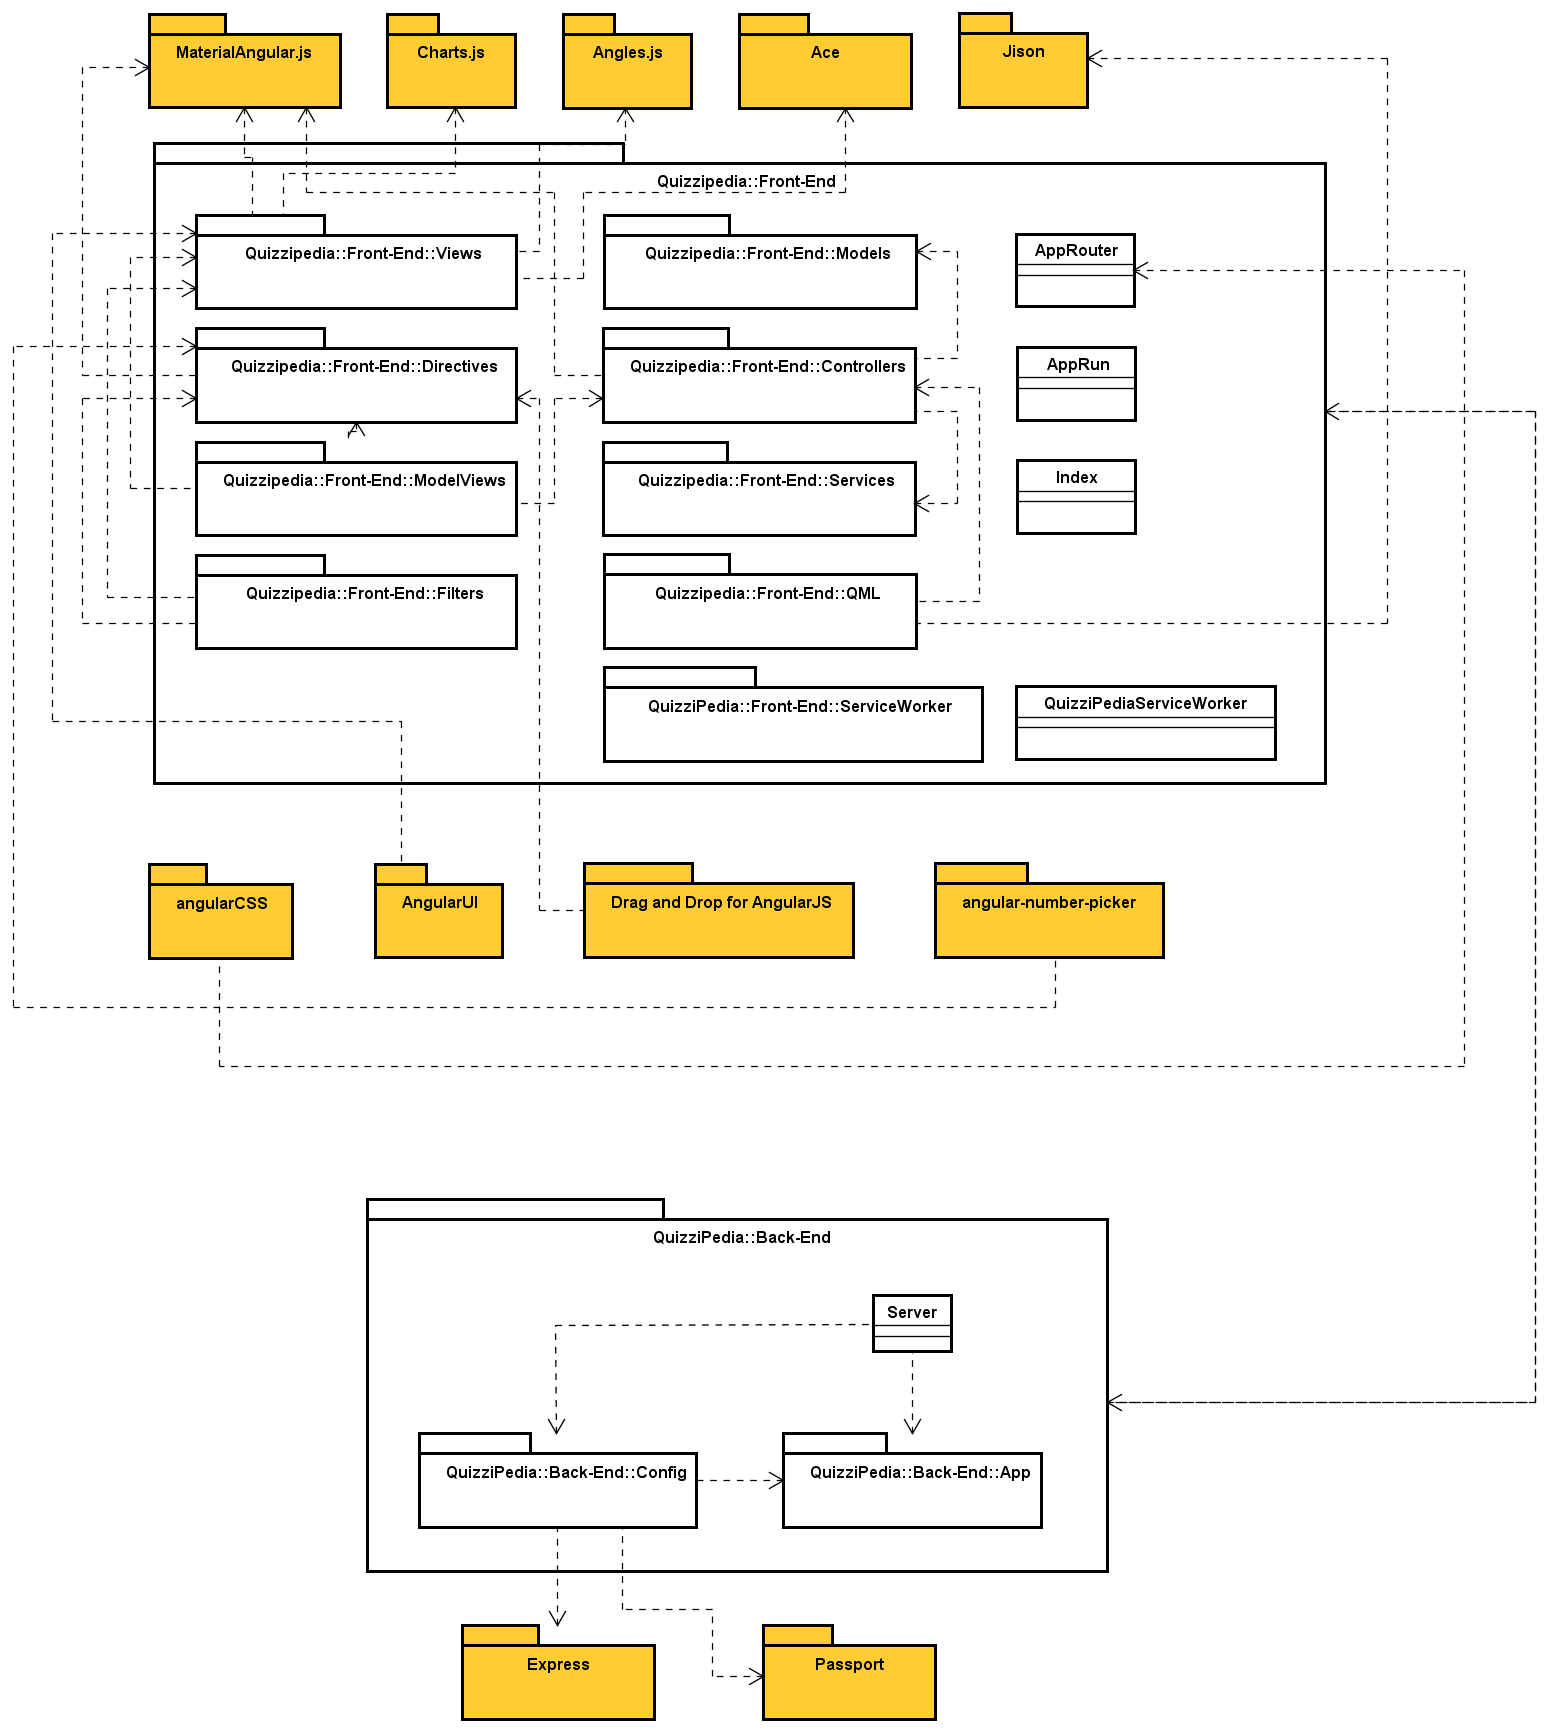
\includegraphics[scale=0.35]{UML/Package/QuizziPedia.png}
	\caption{Architettura}
\end{figure}
\FloatBarrier
\begin{itemize}
	\item \textbf{Descrizione}: architettura ad alto livello dell'applicazione \progetto;
	\item \textbf{Packages contenuti}:
	\begin{itemize}
		\item \texttt{QuizziPedia::Front-End}: \textit{package\ped{G}} contenente i \textit{packages\ped{G}} che compongono il Front-End;
		\item \texttt{QuizziPedia::Back-End}: \textit{package\ped{G}} contenente i \textit{packages\ped{G}} che compongono il Back-End;
		\item \texttt{MaterialAngular.js}: framework per lo sviluppo dei componenti grafici dell'applicazione;
		\item \texttt{Charts.js}: libreria per lo sviluppo dei grafici per la visualizzazione delle statistiche utente;
		\item \texttt{Angles.js}: libreria necessaria per integrare la libreria Charts.js all'interno dell'ambiente \textit{Angular\ped{G}};
		\item \texttt{TextAngular.js}: libreria per la creazione di un editor di testo all'interno delle pagine web per permettere all'utente di creare domande custom in linguaggio \textit{QML\ped{G}};
		\item \texttt{Jison}: è un generatore di parser JavaScript;
		\item \texttt{Express}: framework Web di routing e middleware, con funzionalità sua propria minima: un’applicazione Express è essenzialmente una serie di chiamate a funzioni middleware;
		\item \texttt{Passport}: \textit{middleware\ped{G}} per l'autenticazione in ambiente \textit{Node.js\ped{G}}.
	\end{itemize}
\end{itemize}

\newpage
\section{QuizziPedia::Front-End}
\label{QuizziPedia::Front-End}
\begin{figure}[ht]
	\centering
	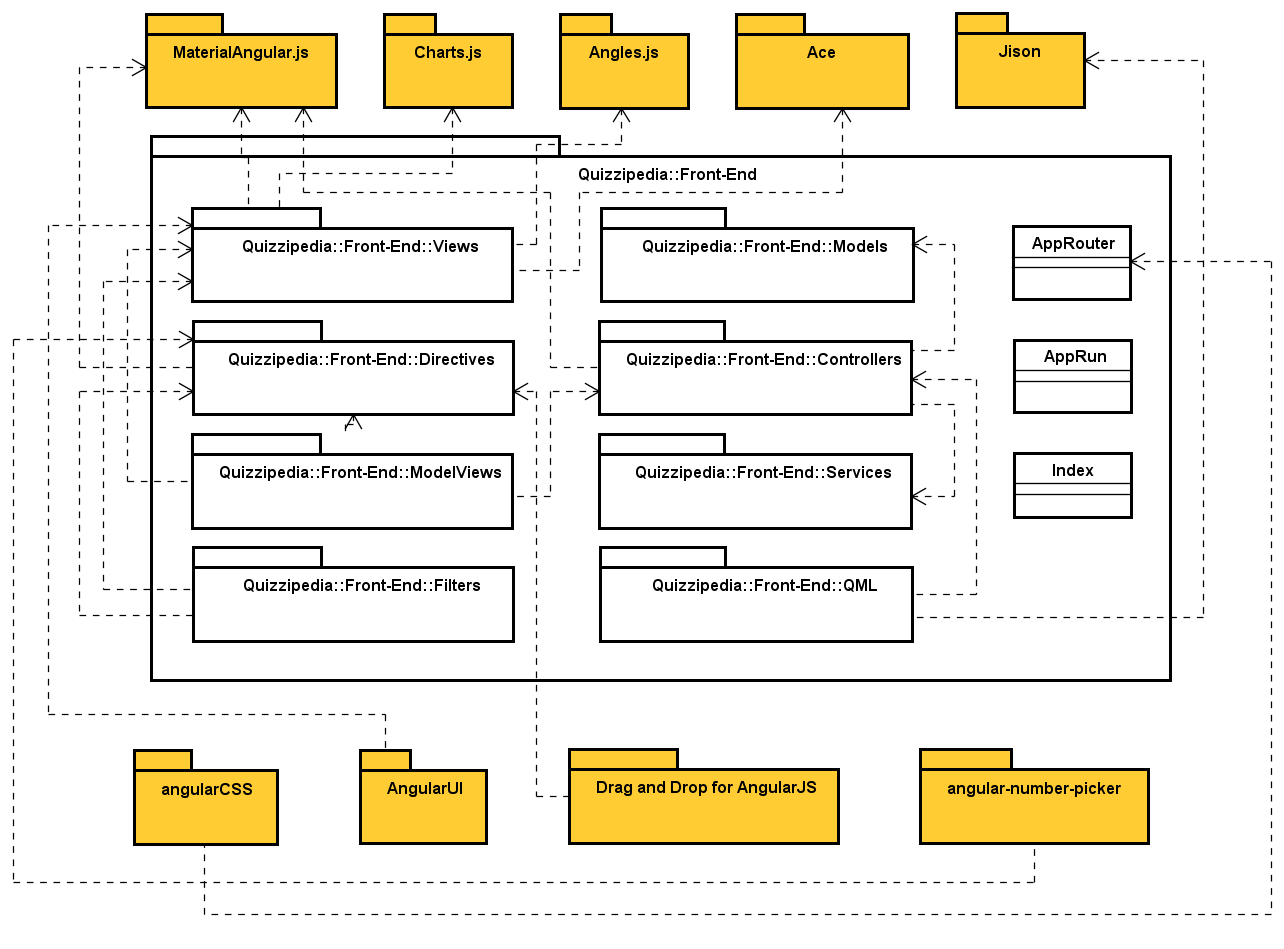
\includegraphics[scale=0.35]{UML/Package/QuizziPedia_Front-end.png}
	\caption{QuizziPedia::Front-End}
\end{figure}
\FloatBarrier
\begin{itemize}
	\item \textbf{Descrizione}: \textit{package\ped{G}} contenente le componenti front-end dell'applicazione;
	\item \textbf{Package contenuti}:
	\begin{itemize}
		\item \texttt{Views}: \textit{package\ped{G}} contenente le \textit{views\ped{G}} front-end dell'applicazione;
		\item \texttt{Controllers}: \textit{package\ped{G}} contenente i \textit{controllers\ped{G}} front-end dell'applicazione;
		\item \texttt{Services}: \textit{package\ped{G}} contenente i \textit{services\ped{G}} front-end dell'applicazione;
		\item \texttt{Models}: \textit{package\ped{G}} contenente le classi che definiscono la business logic dell'applicazione;
		\item \texttt{Directives}: \textit{package\ped{G}} contenente le \textit{directives\ped{G}} front-end dell'applicazione.
	\end{itemize}
	\item \textbf{Classi contenute}:
	\begin{itemize}
		\item \texttt{Index}: \textit{view\ped{G}} generale dell'applicazione. Contiene gli elementi che saranno presenti in ogni pagina dell'applicazione;
		\item \texttt{AppRun}: classe che verifica se l'utente sia autenticato e che abbia le giuste autorizzazioni per la pagina in cui si trova;
		\item \texttt{AppRouter}: classe che gestisce i routes dell'applicazione, utilizza il servizio \$routeProvider per associare ad ogni route un \textit{controller\ped{G}} e una \textit{view\ped{G}}.
	\end{itemize}
\end{itemize}

\newpage
\subsection{QuizziPedia::Front-End::Views}

\label{QuizziPedia::Front-End::Views}
\begin{figure}[ht]
	\centering
	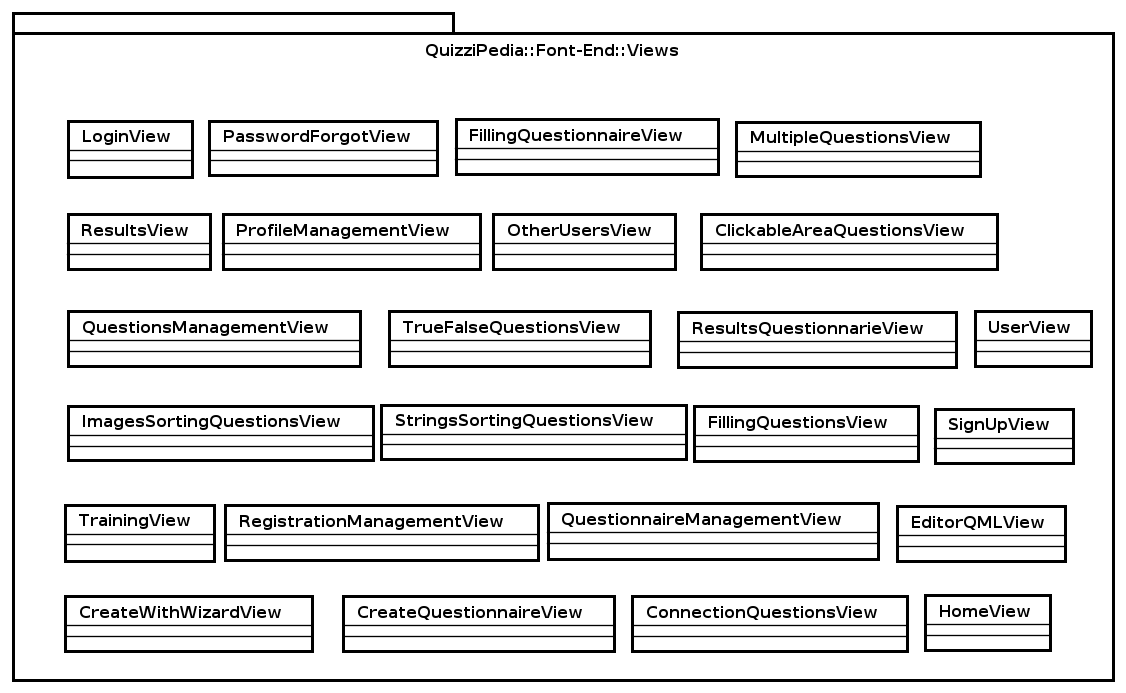
\includegraphics[scale=0.55]{UML/Package/QuizziPedia_Front-End_Views.png}
	\caption{QuizziPedia::Front-End::Views}
\end{figure}\FloatBarrier
\begin{itemize}
	\item \textbf{Descrizione}: package contenente le views front-end dell'applicazione;
	\item \textbf{Padre}: \texttt{Front-End};
	\item \textbf{Interazione con altri componenti}:
	\begin{itemize}
		\item \texttt{Controllers}: package contenente i \textit{controllers\ped{G}} Front-End dell'applicazione;
		\item \texttt{Directives}: package contenente le \textit{directives\ped{G}} Front-End dell'applicazione.
	\end{itemize}
	\item \textbf{Classi contenute}:
	\begin{itemize}
		\item \texttt{LoginView}: classe contenente le form necessarie per effettuare il login. Contiene inoltre un link alla pagina di registrazione e uno alla pagina per il recupero della password;
		\item \texttt{SignUpView}: classe contenente le form dedicate alla registrazione utente. Contiene inoltre un link alla pagina di login;
		\item \texttt{PasswordForgotView}: classe contenente le form necessarie per il recupero della password dimenticata;
		\item \texttt{HomeView}: classe contenente la direttiva per barra di ricerca degli utenti e questionari e il bottone che porterà l'utente nella modalità allenamento;
		\item \texttt{ResultsView}: classe contenente i risultati della ricerca effettuata. Vengono visualizzati sia gli utenti che i questionari trovati;
		\item \texttt{UserView}: contenente le direttive dei dati personali dell'utente, delle sue statistiche relative ai questionari e agli allenamenti effettuati e dei questionari a cui è iscritto;
		\item \texttt{OtherUserView}: classe contenente le direttive dei dati personali e delle statistiche di un utente ricercato;
		\item \texttt{ProfileManagementView}: classe contenente i dati personali che un utente può modificare dopo essersi registrato al sistema;
		\item \texttt{QuestionsManagementView}: classe contenente l'elenco delle domande create;
		\item \texttt{TrueFalseQuestionView}: classe contenente le direttive per creare una domanda vero/falso;
		\item \texttt{MultipleQuestionView}: classe contenente le direttive per creare una domanda a risposta multipla;
		\item \texttt{ConnectionQuestionView}: classe contenente i campi e le direttive per creare una domanda a collegamento;
		\item \texttt{ImagesSortingQuestionView}: classe contenente i campi e le direttive per creare una domanda a ordinamento immagini;
		\item \texttt{StringsSortingQuestionView}: classe contenente i campi e le direttive per creare una domanda a ordinamento stringhe;
		\item \texttt{FillingQuestionsView}: classe contenente i campi e le direttive per creare una domanda a riempimento testo;
		\item \texttt{ClickableAreaQustionView}: classe contenente i campi e le direttive per creare una domanda ad area cliccabile;
		\item \texttt{EditorQMLView}: classe contenente l'editor \textit{QML\ped{G}} per la creazione di domande personalizzate;
		\item \texttt{TrainingView}: classe principale della modalità allenamento; conterrà i vari templates di ogni domanda dell'allenamento;
		\item \texttt{FillingQuestionnaireView}: classe principale per la compilazione del questionario; conterrà i vari templates di ogni domanda appartenente al questionario;
		\item \texttt{QuestionnaireManagementView}: classe principale per la gestione dei questionari;
		\item \texttt{CreateQuestionnaireView}: classe per la creazione del questionario;
		\item \texttt{ResultQuestionnaireView}: classe contenente i risultati conseguiti dagli utenti che hanno compilato il proprio questionario;
		\item \texttt{RegiastrationManagementView}: classe che permette di visualizzare gli utenti iscritti ad un questionario.
	\end{itemize}
\end{itemize}
\newpage
\subsection{QuizziPedia::Front-End::Controllers}

\begin{figure} [ht]
	\centering
	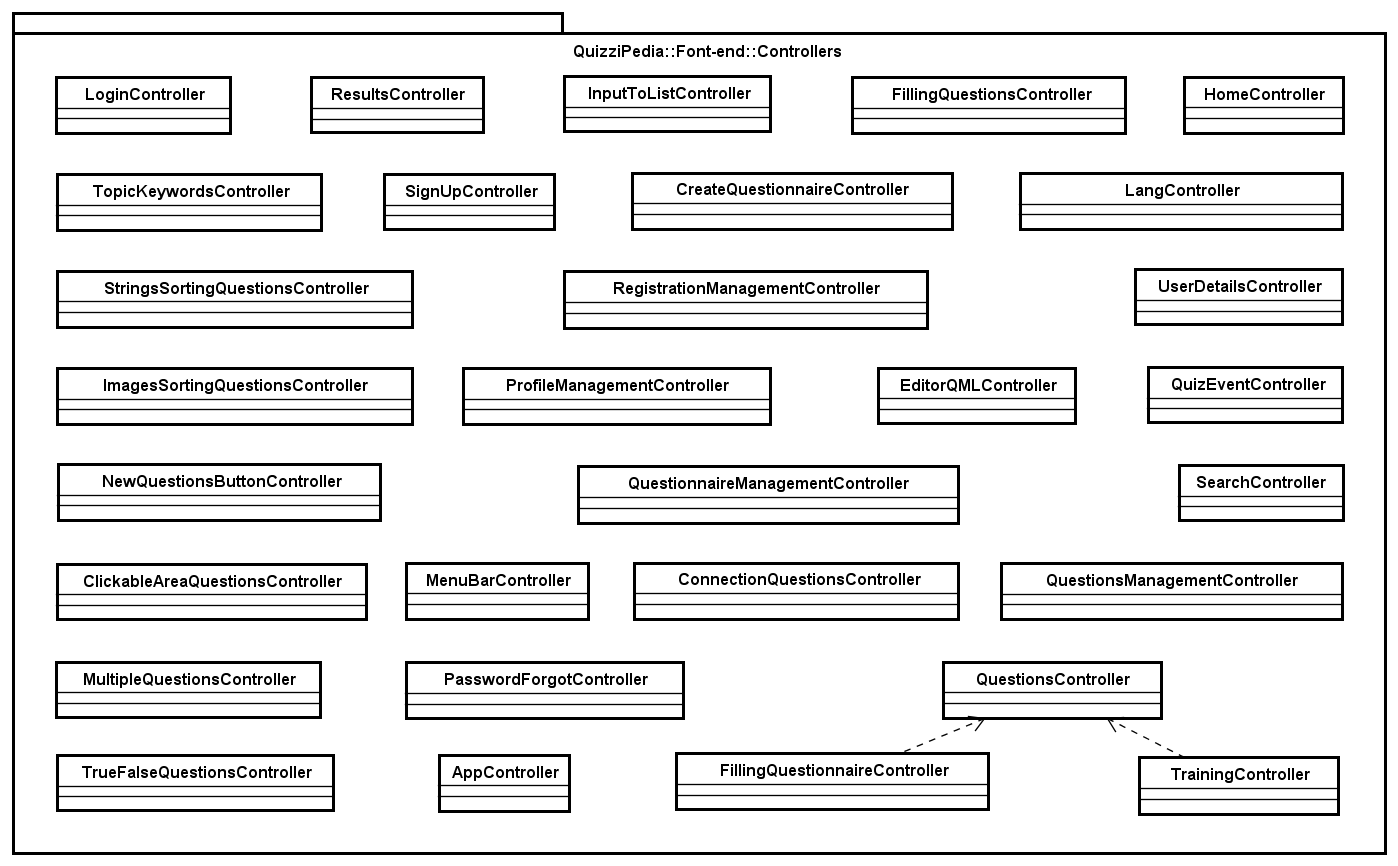
\includegraphics[scale=0.45]{UML/Package/QuizziPedia_Front-End_Controllers.png}
	\caption{QuizziPedia::Front-End::Controllers}
\end{figure} \FloatBarrier

\begin{itemize}
	\item \textbf{Descrizione}: \textit{package\ped{G}} che contiene i controller individuati per la parte front-end dell'applicazione;
	\item \textbf{Padre}: \texttt{Front-End};
	\item \textbf{Interazione con altri componenti}:
	\begin{itemize}
		\item \texttt{Views}: \textit{package\ped{G}} che contiene le \textit{views\ped{G}} dell'applicazione;
		\item \texttt{Models}: \textit{package\ped{G}} che contiene le classi \textit{model\ped{G}} dell'applicazione;
		\item \texttt{Services}: \textit{package\ped{G}} che contiene i \textit{services\ped{G}} dell'applicazione.
	\end{itemize}
	\item \textbf{Classi contenute}:
	\begin{itemize}
		\item \texttt{ClickableAreaQuestionController}: questa classe permette di gestire la creazione e la modifica di una domanda ad area cliccabile;
		\item \texttt{ConnectionQuestionController}: questa classe permette di gestire la creazione e la modifica di una domanda a collegamento;
		\item \texttt{CreateQuesrtionnaireController}: questa classe permette di gestire la creazione di un questionario;
		\item \texttt{EditorQMLController}: questa classe permette di gestire la creazione e la modifica di domande create tramite editor \textit{QML\ped{G}};
		\item \texttt{FillingQuestionnaireController}: questa classe permette di gestire la compilazione del questionario;
		\item \texttt{FillingQuestionsController}: questa classe permette di gestire la creazione e la modifica di una domanda	a riempimento di spazi;
		\item \texttt{HomeController}: questa classe permette di gestire la home page;
		\item \texttt{ImagesSortingQuestionsController}: questa classe permette di gestire la creazione e la modifica di una domanda a ordinamento immagini;
		\item \texttt{InputToListController}: questa classe permette di gestire l'inserimento di una lista di risposte durante la creazione di una domanda;
		\item \texttt{LoginController}: questa classe permette di gestire l'autenticazione dell'utente al sistema;
		\item \texttt{MenuBarController}: questa classe permette di gestire il menù fisso per ogni pagina;
		\item \texttt{MultipleQuestionController}: questa classe permette di gestire la creazione e la modifica di una domanda a risposta multipla;
		\item \texttt{NewQuestionButtonController}: questa classe permette di effettuare il redirect alla pagina di creazione nuova domanda;
		\item \texttt{PasswordForgotController}: questa classe permette di gestire il ripristino della password dimenticata;
		\item \texttt{ProfileManagementController}: questa classe permette di gestire il profilo personale di un utente;
		\item \texttt{QuestionnaireDeatailsController}: questa classe permette di gestire i dettagli di un questionario;
		\item \texttt{QuestionnaireManagementController}: questa classe permette di gestire tutti i questionari creati da un utente;
		\item \texttt{QuestionsController}: questa classe permette di gestire il recupero delle domande per far si che possano essere visualizzate nella modalità allenamento e nella compilazione dei questionari;
		\item \texttt{QuestionsManagementController}: questa classe permette di gestire le domande create dall'utente e di crearne di nuove;
		\item \texttt{QuizEventController}: questa classe permette di reagire ai comandi dell'utente durante la gestione dei suoi questionari;
		\item \texttt{RegistrationManagementController}: questa classe permette di gestire le iscrizione degli utenti ai questionari;
		\item \texttt{ResultQuestionnaireController}: questa classe permette di gestire la visualizzazione dei risultati di un singolo questionario;
		\item \texttt{SearchController}: questa classe permette di gestire la ricerca di questionari e utenti all'interno dell'applicazione;
		\item \texttt{SignUpController}: questa classe permette di gestire la registrazione di un utente al sistema;
		\item \texttt{StatisticsController}: questa classe permette di gestire le statistiche di un utente;
		\item \texttt{StringsSortingQuestionController}: questa classe permette di gestire la creazione e la modifica di una domanda a ordinamento di stringhe;
		\item \texttt{TopicKeywordsController}: questa classe permette di gestire il recupero delle parole chiave di un questionario;
		\item \texttt{TrainingController}: questa classe permette di gestire la modalità allenamento sottoponendo all'utente le giuste domande adatte al suo livello;
		\item \texttt{TrueFalseQuestionController}: questa classe permette di gestire la creazione e la modifica di una domanda	vero/falso;
		\item \texttt{UserDetailsController}: questa classe permette di gestire i dati di un utente da mostrare nella pagina di un profilo.
	\end{itemize} 
\end{itemize}
\newpage
\subsection{QuizziPedia::Front-End::Services}
\begin{figure}[ht]
	\centering
	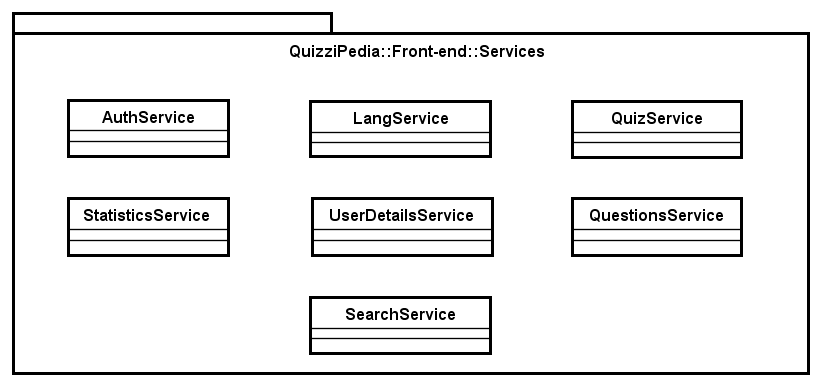
\includegraphics[scale=0.55]{UML/Package/QuizziPedia_Front-End_Services.png}
	\caption{QuizziPedia::Front-End::Services}
\end{figure} \FloatBarrier

\begin{itemize}
	\item \textbf{Descrizione}: package che contiene le classi individuate che permettono la comunicazione del lato front-end con il lato back-end;
	\item \textbf{Padre:} \texttt{Front-End};
	\item \textbf{Interazione con altri componenti:}
	\begin{itemize}
		\item \texttt{Models}: package che contiene le classi \textit{model\ped{G}} dell'applicazione;
		\item \texttt{Controllers}: package che contiene le classi \textit{controller\ped{G}} dell'applicazione.
	\end{itemize}
	\item \textbf{Classi contenute}:
	\begin{itemize}
		\item \texttt{AuthServices}: questa classe permette di gestire la registrazione e l'autenticazione di un utente;
		\item \texttt{LangService}: questa classe permette di gestire la lingua nella quale si è scelto di utilizzare l'applicazione;
		\item \texttt{QuestionsService}: questa classe permette di ottenere domande esistenti e salvare nuove domande;
		\item \texttt{QuizService}: questa classe permette di ottenere i dati di un quiz tramite delle parole chiave inserite dall'utente nella barra di ricerca. Permette inoltre di iscriversi ad un questionario e di scaricare l'intera lista di domande di un questionario a partire dal suo id univoco;
		\item \texttt{SearchService}: questa classe permette di gestire il recupero dei dati dal back-end a seguito di una ricerca effettuata da un utente;
		\item \texttt{StatisticsService}: questa classe permette di ottenere le statistiche dell'utente;
		\item \texttt{UserDetailsService}: questa classe permette di ottenere i dati personali degli utenti.
	\end{itemize} 
\end{itemize}
\newpage

\subsection{QuizziPedia::Front-End::Directives}

\label{QuizziPedia::Front-End::Directives}
\begin{figure} [ht]
	\centering
	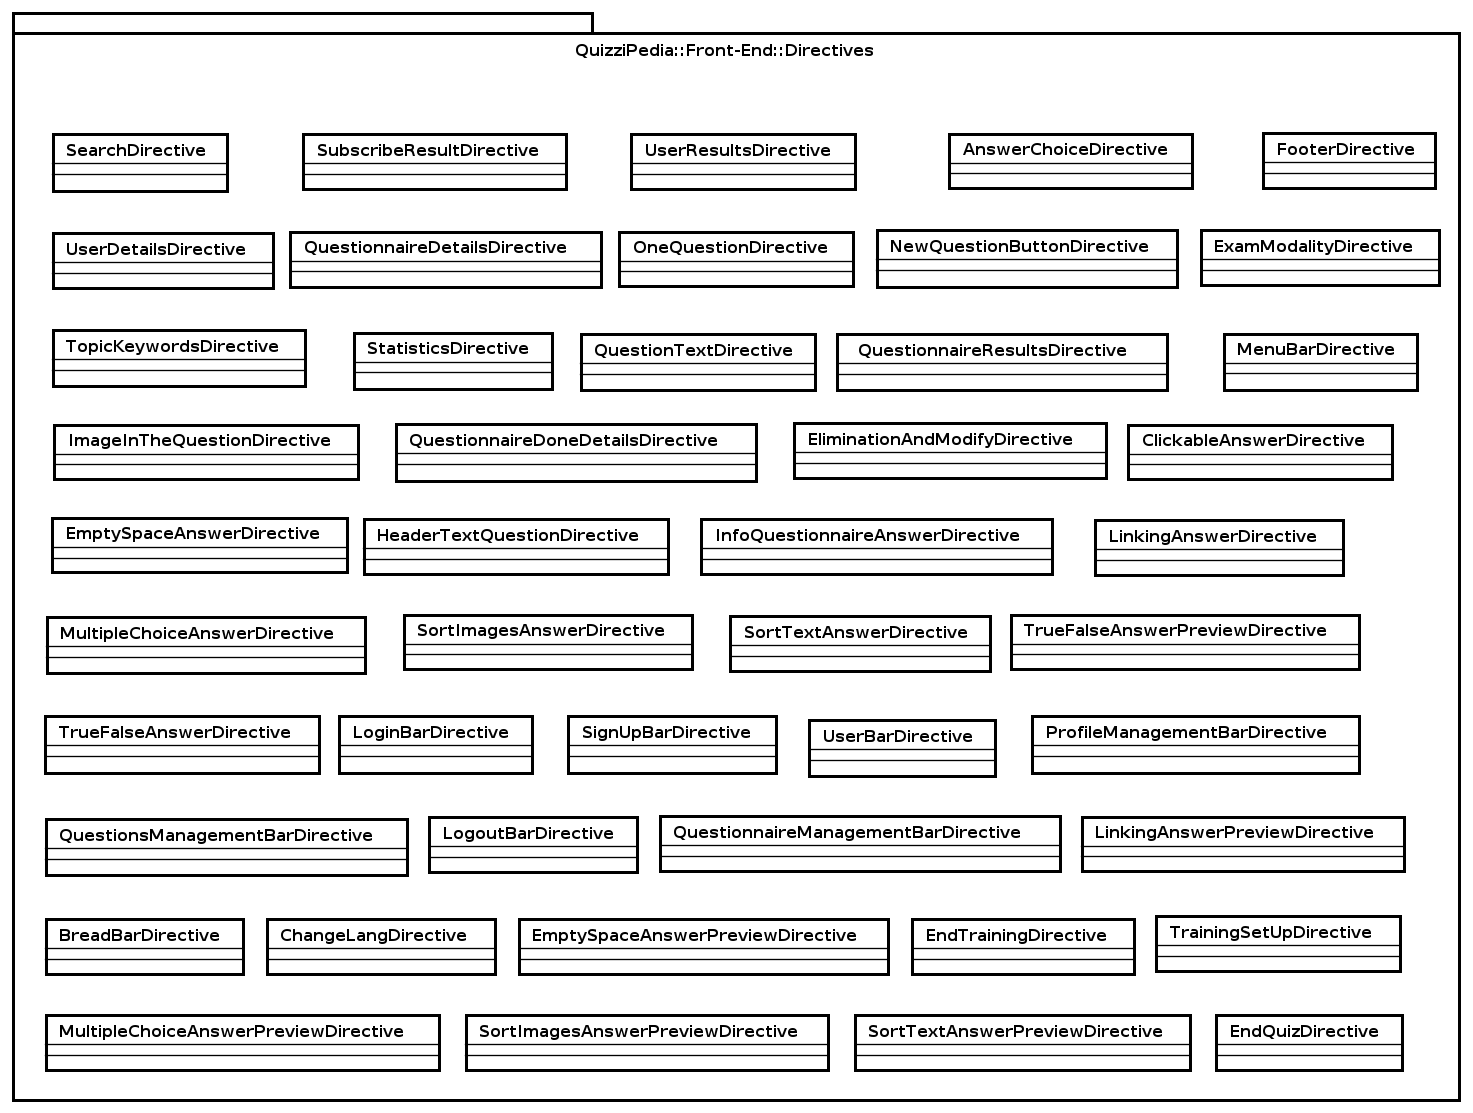
\includegraphics[scale=0.40]{UML/Package/QuizziPedia_Front-End_Directives.png}
	\caption{QuizziPedia::Front-End::Directives}
\end{figure}

\begin{itemize}
	\item \textbf{Descrizione}: package contenente le \textit{directives\ped{G}};
	\item \textbf{Padre}: \texttt{Front-End};
	\item \textbf{Interazione con altri componenti}:
	\begin{itemize}
		\item \texttt{Controllers}: package contenente i \textit{controllers\ped{G}} front-end dell'applicazione;
		\item \texttt{Views}: package contenente le \textit{views\ped{G}} front-end dell'applicazione.
	\end{itemize}
	\item \textbf{Classe contenute}:
	\begin{itemize}
		\item \texttt{EliminationAndModifyDirective}: componente grafico contenente i bottoni per eliminare o modificare un questionario;
		\item \texttt{ExamModalityDirective}: classe contenete i componenti grafici per attivare la modalità esame su un questionario e gestire le iscrizioni;
		\item \texttt{FooterDirective}: classe contenente i componenti grafici del footer dell'applicazione;
		\item \texttt{ImageInTheQuestionDirective}: classe contenente i componenti grafici per l'inserimento dell'immagine	nella creazione delle domande;
		\item \texttt{MenuBarDirective}: rappresenta il menù, presente in ogni pagina dell'applicazione, generato in base agli oggetti passati nello \$scope isolato. Fornisce un pulsante per ogni oggetto ricevuto come parametro, ogni pulsante viene rappresentato con un'icona e con un testo. Al click di un pulsante viene invocata la funzione ad esso associata;
		\item \texttt{OneQuestionDirective}: rappresenta il componente grafico che visualizza all'utente l'anteprima della domanda che ha creato. Eseguendo l'azione di click sul pulsante di modifica sarà possibile modificare tale domanda. All'interno di QuestionsManagementsView verranno stampati a video tanti componenti quanti presenti nello \$scope isolato ad esso associato;
		\item \texttt{NewQuestionButtonDirective}: rappresenta il componente grafico che permette all'utente di posizionarsi nella \textit{view\ped{G}} di creazione di una nuova domanda;
		\item \texttt{QuestionTextDirective}: rappresenta il componente grafico che permette all'utente di scrivere o modificare il testo di una domanda;
		\item \texttt{QuestionnaireDetailsDirective}: rappresenta il componente grafico che permette all'utente di visualizzare la lista di questionari che può compilare;
		\item \texttt{QuestionnaireDoneDetailsDirective}: rappresenta il componente grafico che permette all'utente di visualizzare la lista di questionari che ha già compilato e di conseguenza vederne le valutazioni;
		\item \texttt{QuestionnaireResultsDirective}: rappresenta il componente grafico che permette all'utente autenticato pro di vedere i risultati di chi ha compilato il questionario. Tale componente è contenuto nella lista dei questionari abilitati alla compilazione. É possibile accedere alla lista dei risultati azionando l'evento ad esso collegato;
		\item \texttt{QuestionnaireResultsDirective}: rappresenta il componente grafico che permette all'utente autenticato pro di vedere i risultati di chi ha compilato il questionario. Tale componente è contenuto nella lista dei questionari abilitati alla compilazione. É possibile accedere alla lista dei risultati azionando l'evento ad esso collegato;
		\item \texttt{SearchDirective}: classe che permette di effettuare la ricerca di utenti e questionari;
		\item \texttt{StatisticsDirective}: classe che permette di visualizzare le statistiche di un utente;
		\item \texttt{SubscribeResultDirective}: classe che permette di visualizzare e iscriversi ai questionari ricercati;
		\item \texttt{TopicKeywordsDirective}: classe che permette di gestire l'inserimento dell'argomento e delle	keywords al momento della creazione della domanda;
		\item \texttt{UserDetailsDirective}: classe che permette di visualizzare i dati personali di un utente;
		\item \texttt{UserResultsDirective}: classe che permette di visualizzare la lista degli utenti ricercati dopo aver utilizzato l'apposita funzione di ricerca;
		\item \texttt{ClickableAnswerDirective}: rappresenta il componente grafico che permette all'utente di visualizzare la domanda ad area cliccabile nell'immagine;
		\item \texttt{EmptySpaceAnswerDirective}: rappresenta il componente grafico che permette all'utente di visualizzare l'esercizio a riempimento di spazi vuoti;
		\item \texttt{HeaderTextQuestionDirective}: rappresenta componente grafico che presenta all'utente l'argomento e le parole chiave della domanda che ha a schermo;
		\item \texttt{InfoQuestionnaireDirective}: rappresenta il componente grafico che permette all'utente di visualizzare le informazioni principali del questionario che si sta per svolgere;
		\item \texttt{LinkingAnswerDirective}: rappresenta componente grafico che permette all'utente di visualizzare la domanda di collegamento;
		\item \texttt{MultipleChoiceAnswerDirective}: rappresenta componente grafico che permette all'utente di visualizzare la domanda a risposta multipla;
		\item \texttt{SortImagesAnswerDirective}: rappresenta il componente grafico che permette all'utente di visualizzare la domanda ad ordinamento di immagini;
		\item \texttt{SortTextAnswerDirective}: rappresenta il componente grafico che permette all'utente di visualizzare la domanda ad ordinamento di stringhe;
		\item \texttt{TrainingSetUpDirective}: rappresenta componente grafico che permette all'utente di selezionare l'argomento e le parole chiave per iniziare un allenamento con queste caratteristiche;
		\item \texttt{TrueFalseAnswerDirective}: rappresenta il componente grafico che permette all'utente di visualizzare la domanda vero e falso;
		\item \texttt{LoginBarDirective}: directive contenente il componente che permette di effettuare il redirect alla pagina di login;
		\item \texttt{SignUpBarDirective}: directive contenente il componente che permette di effettuare il redirect alla pagina di registrazione;
		\item \texttt{UserBarDirective}: directive contenente il componente che permette di effettuare il redirect alla pagina di visualizzazione profilo;
		\item \texttt{ProfileManagementBarDirective}: directive contenente il componente che permette di effettuare il redirect alla pagina di gestione del profilo;
		\item \texttt{QuestionsManagementBarDirective}: directive contenente il componente che permette di effettuare il redirect alla pagina di gestione delle domande;
		\item \texttt{LogoutBarDirective}: directive contenente il componente che permette di effettuare il logout dal sistema;
		\item \texttt{QuestionnaireManagementBarDirective}: directive contenente il componente che permette di effettuare il redirect alla pagina di gestione dei questionari.
	\end{itemize}
\end{itemize}
%\newpage

\subsection{QuizziPedia::Front-End::Models}

	\label{QuizziPedia::Front-End::Models}
	
	\begin{figure}[ht]
		\centering
		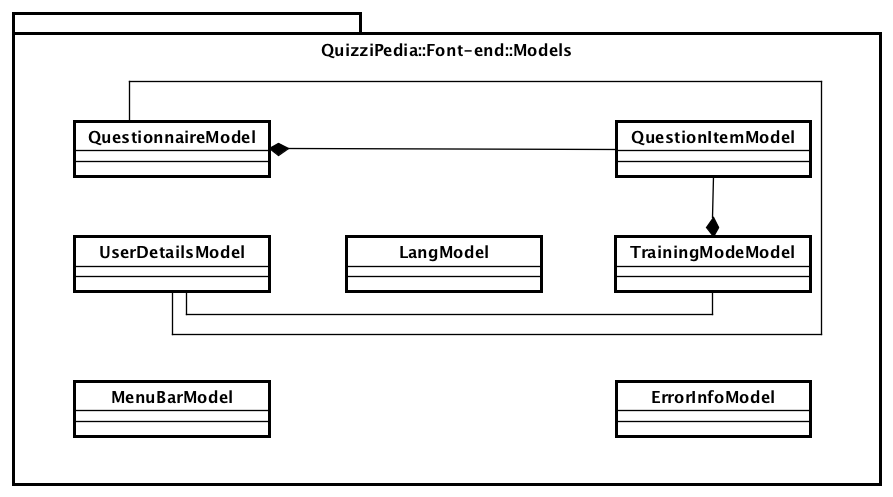
\includegraphics[scale=0.5,keepaspectratio]{UML/Package/QuizziPedia_Front-End_Models.png}
		\caption{QuizziPedia::Front-End::Models}
	\end{figure} \FloatBarrier

		\begin{itemize}
			\item \textbf{Descrizione}: \textit{package\ped{G}} contenente le classi che definiscono la business logic dell'applicazione;
			\item \textbf{Padre}: \texttt{Front-End};
			\item \textbf{Iterazioni con altri componenti}: 
				\begin{itemize}				
					\item \texttt{Controllers}: \textit{package\ped{G}} contenente i controllers front-end dell'applicazione;
					\item \texttt{Directives}: \textit{package\ped{G}} contenente le directives front-end dell'applicazione;
					\item \texttt{Models}: \textit{package\ped{G}} contenente le classi che definiscono la business logic dell'applicazione;
					\item \texttt{Services}: \textit{package\ped{G}} che contiene le classi individuate che permettono la comunicazione del lato front-end con il lato back-end attraverso l'architettura \textit{REST\ped{G}}.
				\end{itemize}
			\item \textbf{Classi contenute}:
			\begin{itemize}
				\item \texttt{UserDetailsModel}: rappresenta un utente. Contiene tutte le informazioni necessarie alla presentazione del contenuto di un utente sia nella visualizzazione che nella gestione di un profilo;
				\item \texttt{TrainingModeModel}: rappresenta un allenamento. Contiene tutte le informazioni necessarie alla presentazione del contenuto di un allenamento;
				\item \texttt{QuestionnaireModel}: rappresenta un questionario. Contiene tutte le informazioni necessarie alla presentazione del contenuto del questionario;
				\item \texttt{QuestionItemModel}: rappresenta una domanda. Contiene tutte le informazioni necessarie alla presentazione del contenuto della domanda;
				\item \texttt{MenuBarModel}: questa classe racchiude i dati necessari per la creazione dinamica della barra menù posizionata in modo fisso su ogni pagina;
				\item \texttt{LangModel}: rappresenta le informazioni per la giusta traduzione dell'applicazione;
				\item \texttt{ErrorInfoModel}: rappresenta le informazioni di un errore che si è verificato eseguendo una determinata operazione;
			\end{itemize}
		\end{itemize}

\newpage
\section{Specifica del Back-End}
\subsection{QuizziPedia::Back-End}
\subsubsection{Informazioni generali}
\label{QuizziPedia::Back-End}
\begin{figure}
	\centering
	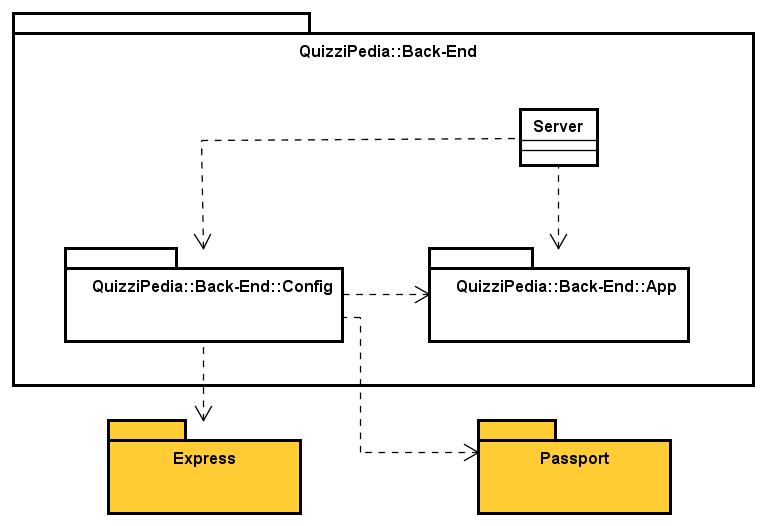
\includegraphics[scale=0.45]{UML/Package/QuizziPedia_Back-End.png}
	\caption{QuizziPedia::Back-End}
\end{figure}

	\begin{itemize}
		\item \textbf{Descrizione} \\ Package contenenti le componenti della parte back-end dell' applicazione.
		\item \textbf{Package contenuti}
		\begin{itemize}
			\item App \\
			Package\ped{G} contenente le componenti del server che implementano il \textit{pattern MVC\ped{G}}.
			\item Config \\
			Package\ped{G} contenente le componenti di configurazione del server\ped{G}.
		\end{itemize}
	\end{itemize}
\subsubsection{Classi}
	\paragraph{QuizziPedia::Back-End::Server}
	\begin{itemize}
		\item \textbf{Descrizione}
		\item \textbf{Utilizzo}
		\item \textbf{Relazioni con altre classi}
		\item \textbf{Attributi}
		\item \textbf{Metodi}
	\end{itemize}

\subsection{QuizziPedia::Back-End::Connection}
\subsubsection{Informazioni generali}
\subsubsection{Classi}

\subsection{QuizziPedia::Back-End::App}
\subsubsection{Informazioni generali}
\label{QuizziPedia::Back-End::App}
\begin{figure}
	\centering
	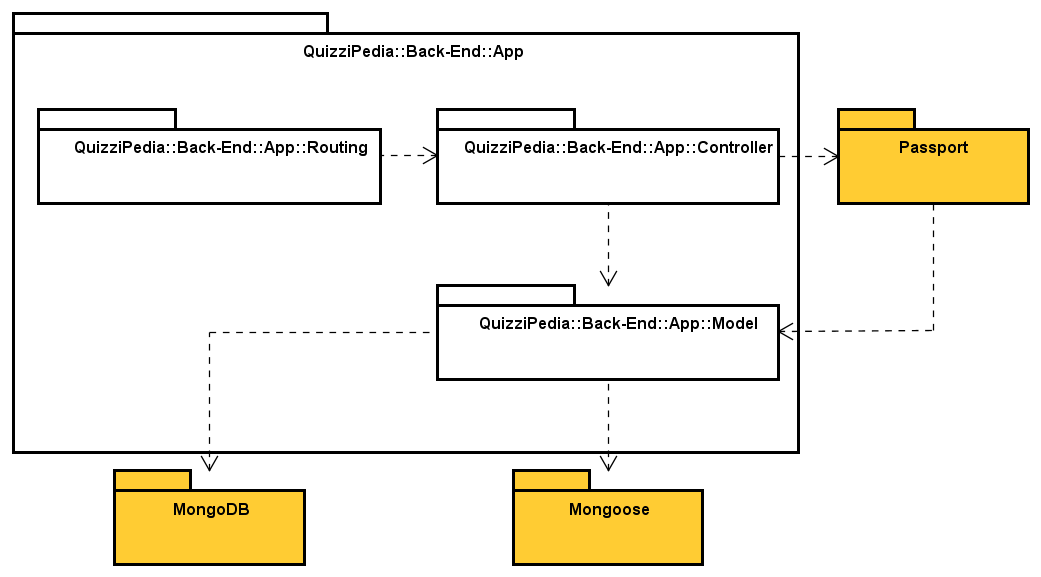
\includegraphics[scale=0.45]{UML/Package/QuizziPedia_Back-End_App.png}
	\caption{QuizziPedia::Back-End::App}
\end{figure}
	\begin{itemize}
		\item \textbf{Descrizione} \\
		Package contenente le componenti del server che implementano il \textit{pattern\ped{G} MVC\ped{G}};
		\item \textbf{Padre} \\ Back-End;
		\item \textbf{Interazioni con altri componenti}
			\begin{itemize}
				\item Congif \\
				Package contenente le componenti di configurazione del server;
			\end{itemize}
		\item \textbf{Package contenuti}
			\begin{itemize}
				\item Controllers \\
				Package che contiene i controllers di Express, definisce la logica dell'applicazione;
				\item Models \\
				Package che contiene le classi che definiscono il model dell'applicazione. Queste classi cono definite come classi schema di \textit{Mongoose\ped{G}}, il quale permette di utilizzare \textit{MongoDB\ped{G}} tramite degli oggetti;
				\item Routers \\
				Package contenente i routers della componente back-end dell'applicazione. Contiene i file di configurazione relativi al routing delle richieste del client, ossia i routers di Express.
			\end{itemize}
	\end{itemize}
	
\subsection{QuizziPedia::Back-End::App::Controllers}
\subsubsection{Informazioni generali}
	\begin{itemize}
		\item \textbf{Descrizione} \\
		\item \textbf{Padre} \\
		\item \textbf{Interazioni con altri componenti} \\
		\item \textbf{Package contenuti}
	\end{itemize}
\subsubsection{Classi}
\paragraph{QuizziPedia::Back-End::App::Controllers::NOMECLASSE}
	\begin{itemize}
		\item \textbf{Descrizione} \\
		\item \textbf{Utilizzo} \\
		\item \textbf{Relazioni con altre classi} \\
		\item \textbf{Metodi} \\
	\end{itemize}


\subsection{QuizziPedia::Back-End::App::Models}
\subsubsection{Informazioni generali}
\subsubsection{Classi}
\paragraph{QuizziPedia::Back-End::App::Models::NOMECLASSE}
\begin{itemize}
	\item \textbf{Descrizione} \\
	\item \textbf{Utilizzo} \\
	\item \textbf{Relazioni con altre classi} \\
	\item \textbf{Metodi} \\
\end{itemize}

\subsection{QuizziPedia::Back-End::App::Routers}
\subsubsection{Informazioni generali}
\subsubsection{classi}
\paragraph{QuizziPedia::Back-End::App::Routers::NOMECLASSE}
	\begin{itemize}
		\item \textbf{Descrizione} \\
		\item \textbf{Utilizzo} \\
		\item \textbf{Relazioni con altre classi} \\
		\item \textbf{Metodi} \\
<<<<<<< HEAD
	\end{itemize}
=======
	\end{itemize}
>>>>>>> origin/master

\section{Diagrammi di sequenza}
\subsection{Back-End}

\subsubsection{Gestione generale delle richieste}

\subsubsection{Richieste REST}
\paragraph{GET /:lang}
\begin{itemize}
\item \textbf{Successo}:\\
Questo scenario rappresenta il successo di una richiesta di keywords inerenti alla lingua impostata che impone, come vincolo per poter essere effettuata, che l'utente non sia autenticato e non possieda già un account nel sistema.  
\label{Procedura di traduzione}
\begin{figure}[ht]
	\centering
	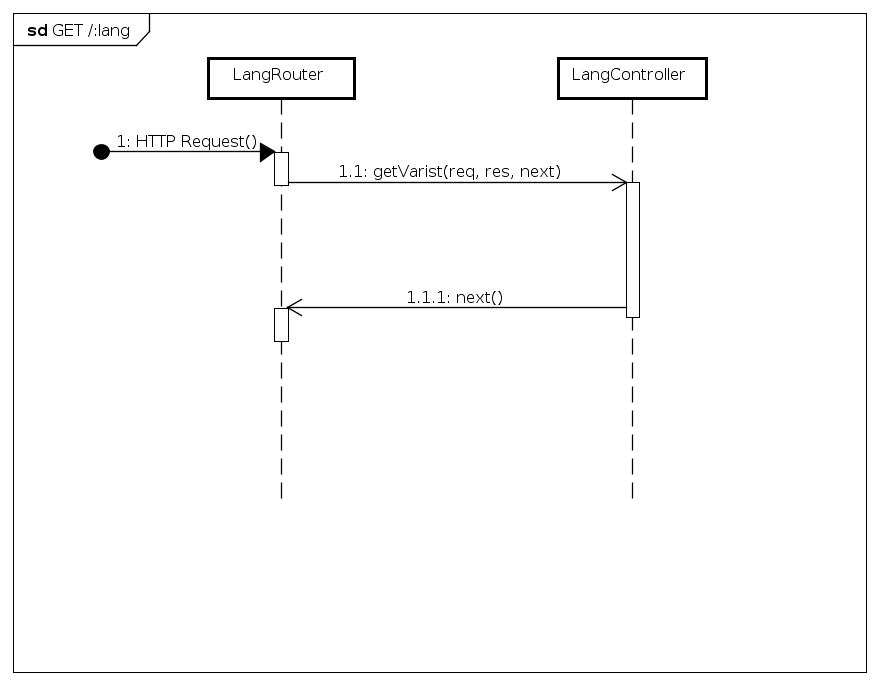
\includegraphics[scale=0.40]{UML/DiagrammiDiSequenza/Back-end/GET_lang_success.png}
	\caption{GET /:lang}
\end{figure}
\FloatBarrier

\item \textbf{Fallimento}:\\
Quando viene effettuata una richiesta di traduzione in una lingua non riconosciuta dal sistema viene sollevato un errore. Tale scenario rappresenta il fallimento di una richiesta di traduzione che impone, come vincolo per poter essere effettuata, che l'utente non sia autenticato e non possieda già un account nel sistema. In questo caso il modulo \texttt{LangController} invia \texttt{next(error)} per il fallimento di tale vincolo al router il quale avrà compito di reinstradarlo (indirizzandolo verso \texttt{ErrorHandler}).
 
\label{Fallimento della procedura di traduzione}
\begin{figure}[ht]
	\centering
	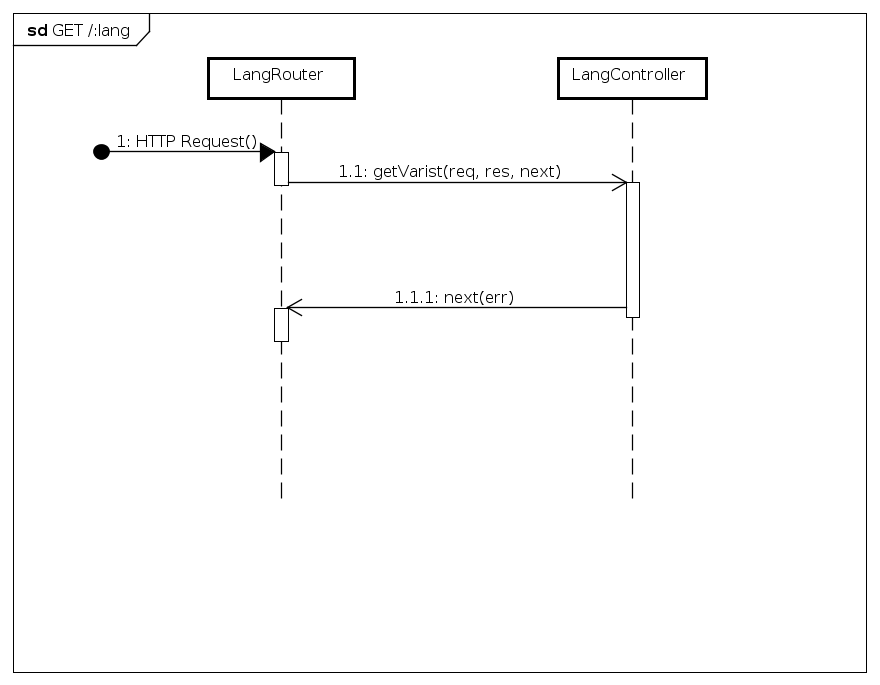
\includegraphics[scale=0.40]{UML/DiagrammiDiSequenza/Back-end/GET_lang_failure.png}
	\caption{GET /:lang}
\end{figure}
\FloatBarrier
\end{itemize}


\paragraph{POST /:lang/signup}
\begin{itemize}
\item \textbf{Successo}:\\
Questo scenario rappresenta il successo di una richiesta di registrazione che impone, come vincolo per poter essere effettuata, che l'utente non sia autenticato e non possieda già un account nel sistema. La registrazione dell'utente nel sistema viene effettuata tramite \textit{Passport\ped{G}} creando ed inserendo un nuovo \textit{document} all'interno della collection User.

\label{Procedura di registrazione}
\begin{figure}[ht]
	\centering
	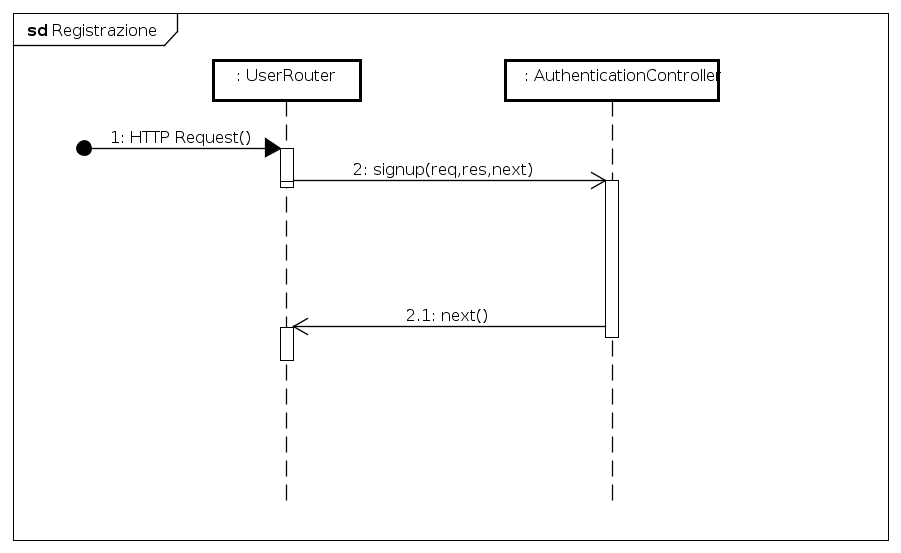
\includegraphics[scale=0.40]{UML/DiagrammiDiSequenza/Back-end/POST__lang_signup_success.png}
	\caption{POST /:lang/signup}
\end{figure}
\FloatBarrier

\item \textbf{Fallimento}:\\
Quando un utente effettua una richiesta di registrazione e cerca di inserire dei dati già presenti del \textit{database\ped{G}} viene sollevato un errore. Tale scenario rappresenta il fallimento di una richiesta di registrazione che impone, come vincolo per poter essere effettuata, che l'utente non sia autenticato e non possieda già un account nel sistema. In questo caso il modulo \texttt{AuthenticationController} invia \texttt{next(error)} per il fallimento di tale vincolo al router il quale avrà compito di reinstradarlo (indirizzandolo verso \texttt{ErrorHandler}).

\label{Fallimento della procedura di registrazione}
\begin{figure}[ht]
	\centering
	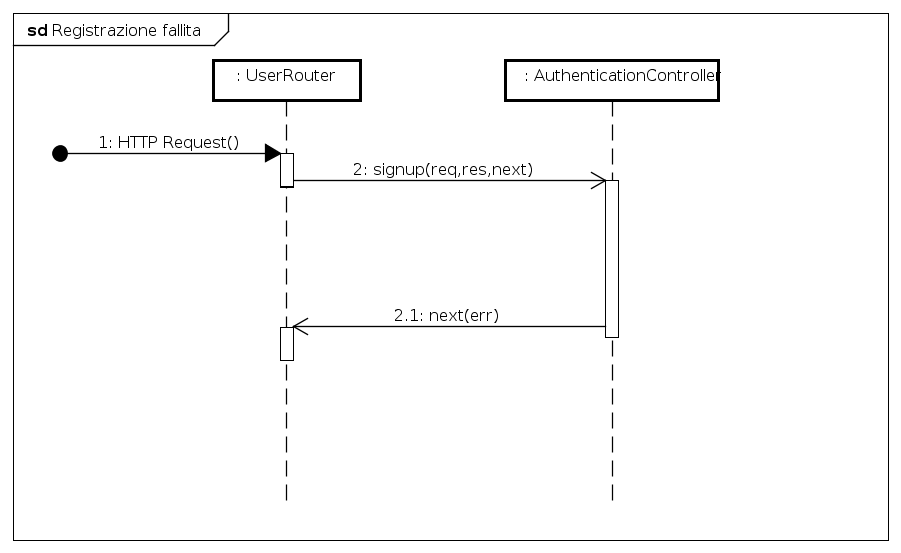
\includegraphics[scale=0.40]{UML/DiagrammiDiSequenza/Back-end/POST__lang_signup_failure.png}
	\caption{Fallimento della procedura di registrazione}
\end{figure}
\FloatBarrier

\end{itemize}

\paragraph{POST /:lang/signin}
\begin{itemize}
\item \textbf{Successo}:\\
La maggior parte delle richieste alle risorse rese disponibili dalle \textit{API\ped{G}} del \textit{server\ped{G}} possono essere effettuate solamente da un \textit{utente autenticato}. Tale scenario rappresenta il successo di una richiesta di \textit{login}, che impone come vincolo per poter essere effettuata, che l'utente abbia un account nel sistema, ma che non sia già autenticato. La \textit{login} dell'utente viene effettuata tramite \textit{Passport\ped{G}}.

\label{Procedura di autenticazione}
\begin{figure}[ht]
	\centering
	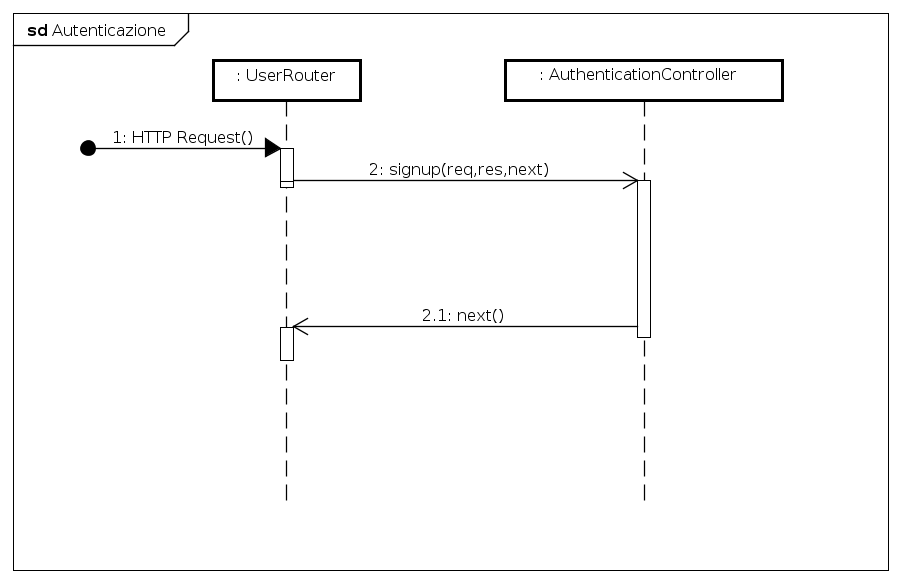
\includegraphics[scale=0.40]{UML/DiagrammiDiSequenza/Back-end/POST__lang_signin_success.png}
	\caption{POST /:lang/signin}
\end{figure}
\FloatBarrier
 
\item \textbf{Fallimento}:\\
La maggior parte delle richieste alle risorse rese disponibili dalle \textit{API\ped{G}} del \textit{server\ped{G}} possono essere effettuate solamente da un \textit{utente autenticato}. Tale scenario rappresenta il fallimento della richiesta di \textit{login}, che può avvenire nel caso sia stia cercando di autenticare un utente non registrato. In questo caso il modulo \texttt{AuthenticationController} invia \texttt{next(error)} al router, il quale avrà compito di reinstradarlo (indirizzandolo verso \texttt{ErrorHandler}).

\label{Fallimento della procedura di autenticazione}
\begin{figure}[ht]
	\centering
	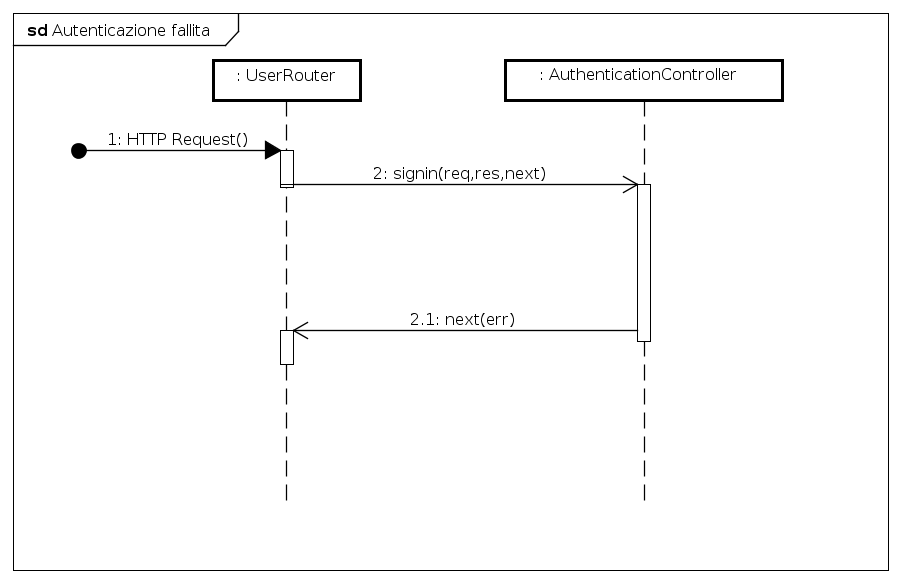
\includegraphics[scale=0.40]{UML/DiagrammiDiSequenza/Back-end/POST__lang_signin_failure.png}
	\caption{Fallimento della procedura di autenticazione}
\end{figure}
\FloatBarrier

\end{itemize}

\paragraph{POST /:lang/signout}
\begin{itemize}
\item \textbf{Successo}
% descrizione diagramma e UML
\item \textbf{Fallimento}
% descrizione diagramma e UML
\end{itemize}

\paragraph{GET /:lang/loggedin}
\begin{itemize}
\item \textbf{Successo}:\\
Questo scenario rappresenta il successo di una richiesta di controllo di sessione che non impone alcun vincolo per poter essere effettuata. Il controllo di sessione dell'utente nel sistema viene effettuata tramite il modulo \texttt{SessionController} che invia \texttt{next()} al router, per indicare il successo dell'operazione .

\label{Procedura di controllo di sessione}
\begin{figure}[ht]
	\centering
	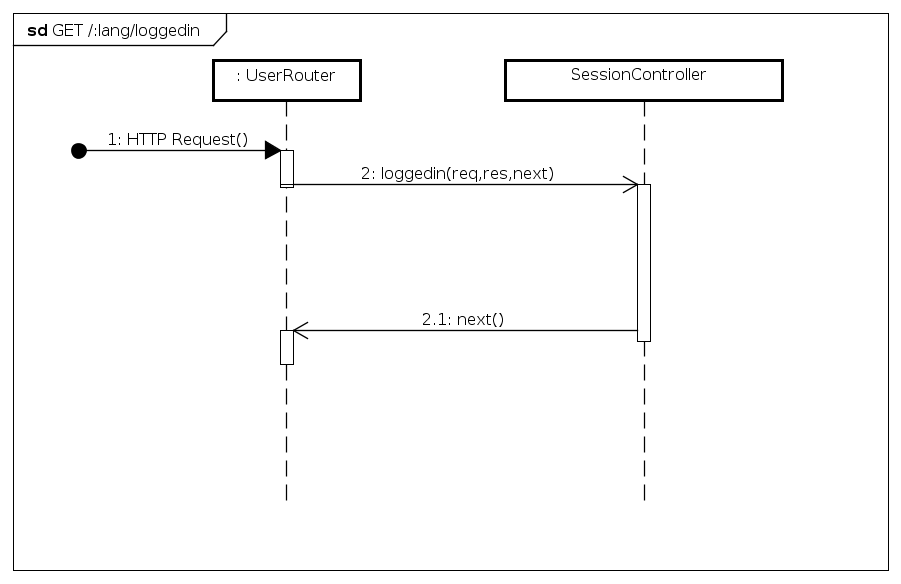
\includegraphics[scale=0.40]{UML/DiagrammiDiSequenza/Back-end/GET__lang_loggedin_success.png}
	\caption{Procedura di controllo di sessione}
\end{figure}
\FloatBarrier
 
\item \textbf{Fallimento}:\\
Questo scenario rappresenta il fallimento di una richiesta di controllo di sessione che non impone alcun vincolo per poter essere effettuata. Il controllo di sessione dell'utente nel sistema viene effettuata tramite il modulo \texttt{SessionController}, che in caso di fallimento, invia \texttt{next(err)} al router,  il quale avrà compito di reinstradarlo (indirizzandolo verso \texttt{ErrorHandler}).

\label{Fallimento della procedura di controllo di sessione}
\begin{figure}[ht]
	\centering
	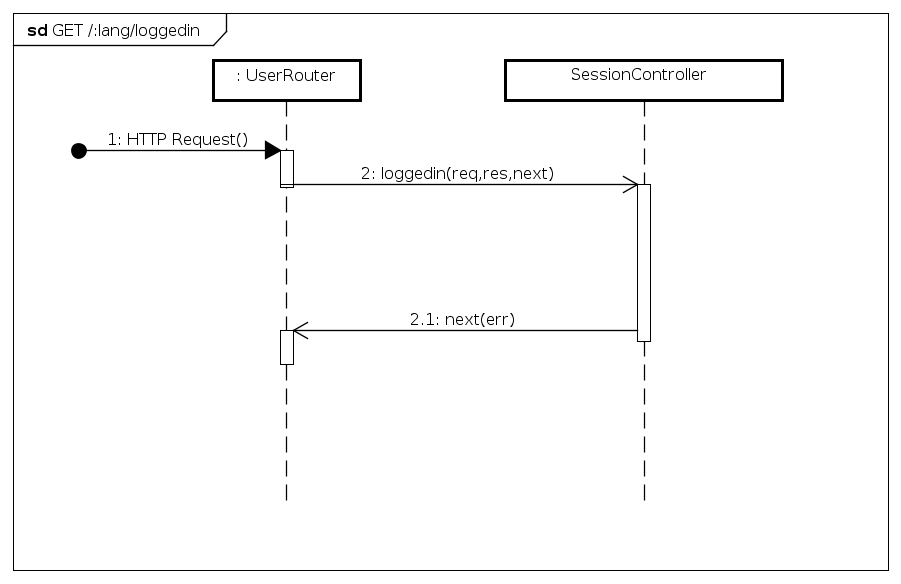
\includegraphics[scale=0.40]{UML/DiagrammiDiSequenza/Back-end/GET__lang_loggedin_failure.png}
	\caption{Fallimento della procedura di controllo di sessione}
\end{figure}
\FloatBarrier

\end{itemize}


\paragraph{POST /:lang/recovery}
\begin{itemize}
\item \textbf{Successo}: quando un utente registrato dimentica la propria password ha la possibilità di accedere al proprio account facendosi inviare una nuova password nell'indirizzo email utilizzato durante la registrazione. Questo scenario rappresenta il successo di una procedura di \textit{recovery} per password dimenticata con vincolo che l'utente sia registrato, ma non autenticato. Il sistema dovrà occuparsi di generare un password, inviarla all'indirizzo email dell'utente e di cambiarla nel suo rispettivo account.

\label{Procedura di recupero password}
\begin{figure}[ht]
	\centering
	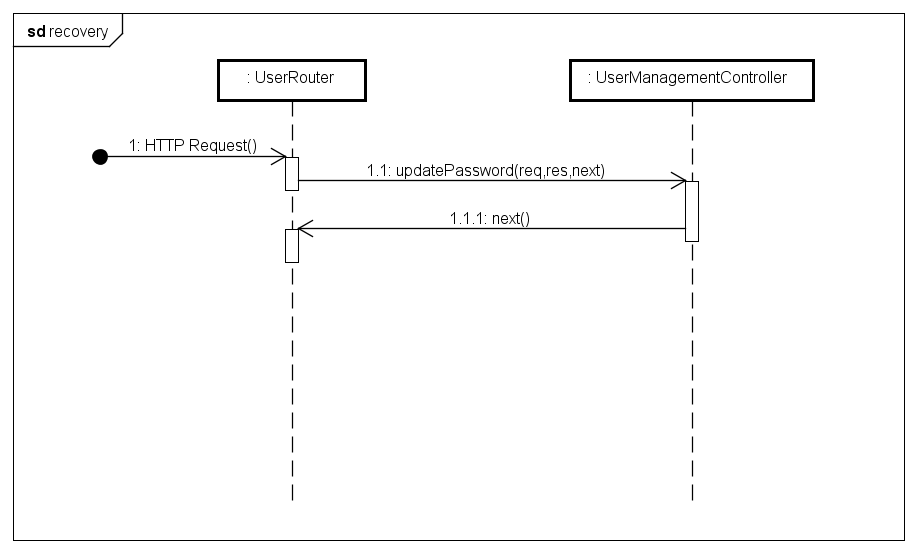
\includegraphics[scale=0.40]{UML/DiagrammiDiSequenza/Back-end/POST__lang_recovery_success.png}
	\caption{Procedura di recupero password}
\end{figure}
\FloatBarrier

\item \textbf{Fallimento} quando un utente richiede un recupero della password inserendo una email non presente nel sistema, viene sollevato un errore. Tale scenario rappresenta il fallimento di una richiesta di recupero della password che impone, come vincolo per poter essere effettuata, che l'utente non sia autenticato. In questo caso il modulo \texttt{AuthenticationController} invia \texttt{next(error)} per il fallimento di tale vincolo al router, il quale avrà compito di reinstradarlo (indirizzandolo verso \texttt{ErrorHandler}).

\label{Fallimento procedura di recupero password}
\begin{figure}[ht]
	\centering
	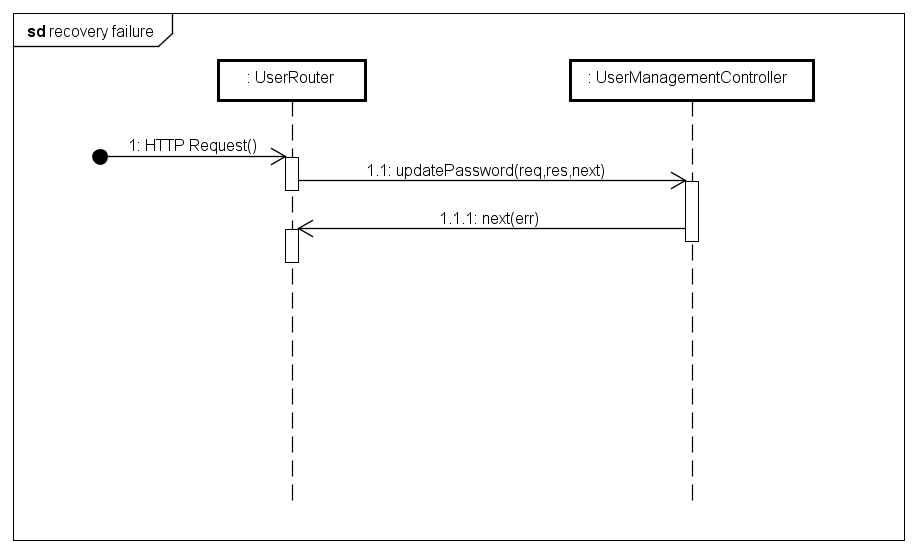
\includegraphics[scale=0.40]{UML/DiagrammiDiSequenza/Back-end/POST__lang_recovery_failure.png}
	\caption{Fallimento della procedura di recupero della password}
\end{figure}
\FloatBarrier

\end{itemize}

\paragraph{DELETE /:lang/user/:userId}
\begin{itemize}
\item \textbf{Successo}: \\
Questo scenario rappresenta il successo di una richiesta di eliminazione account che impone, come vincolo per poter essere effettuata, che l'utente sia autenticato al sistema.  
In questo caso il modulo \texttt{UserManagementController} invia \texttt{next()} per indicare il successo dell'operazione e successivamente verrà effettuata la logout() per completare interamente l'operazione.
\label{Procedura di eliminazione account}
\begin{figure}[ht]
	\centering
	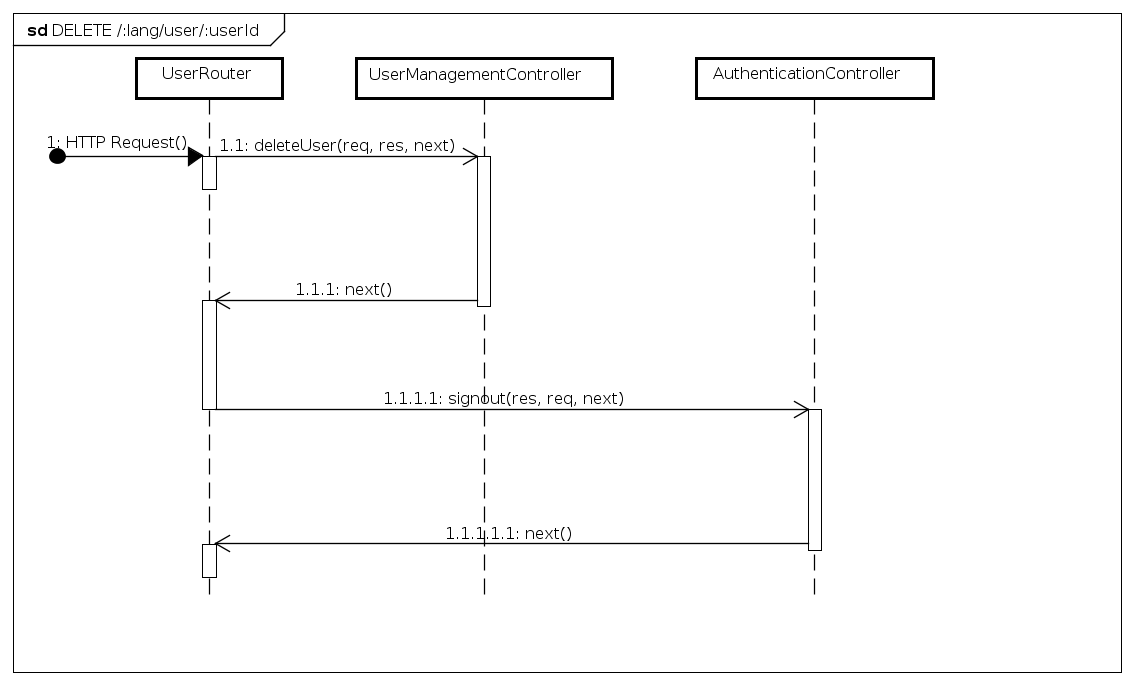
\includegraphics[scale=0.40]{UML/DiagrammiDiSequenza/Back-end/DELETE_LangUserUseridSuccess.png}
	\caption{Procedura di eliminazione account}
\end{figure}
\FloatBarrier

\item \textbf{Fallimento}: \\
Quando viene effettuata una richiesta di eliminazione account sollevando un errore. Tale scenario rappresenta il fallimento di una richiesta di eliminazione account che impone, come vincolo per poter essere effettuata, che l'utente sia autenticato al sistema. In questo caso il modulo \texttt{UserManagementController} invia \texttt{next(error)} per il fallimento di tale vincolo al router il quale avrà compito di reinstradarlo (indirizzandolo verso \texttt{ErrorHandler}).

\label{Fallimento della procedura di eliminazione account}
\begin{figure}[ht]
	\centering
	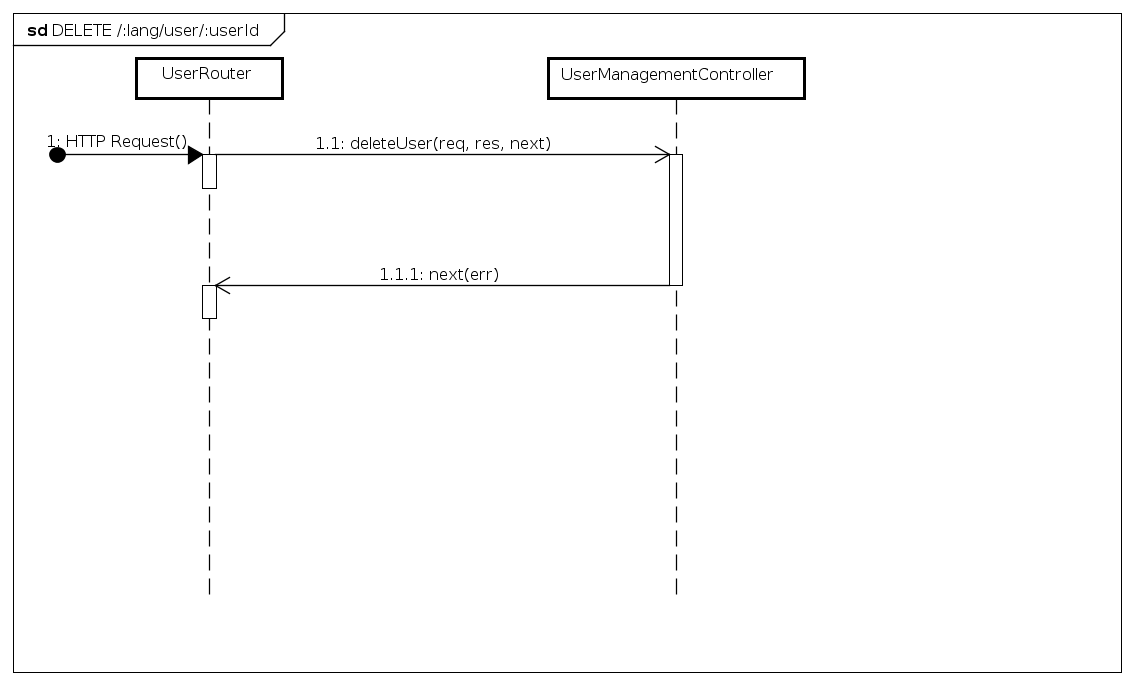
\includegraphics[scale=0.40]{UML/DiagrammiDiSequenza/Back-end/DELETE_LangUserUseridFailure.png}
	\caption{Fallimento della procedura di eliminazione account}
\end{figure}

\FloatBarrier
\end{itemize}

\paragraph{GET /:lang/user/:userId}
\begin{itemize}
\item \textbf{Successo}:\\
Questo scenario rappresenta il successo di una richiesta di visualizzazione dei dati dell'utente che impone, come vincolo per poter essere effettuata, che l'utente sia autenticato al sistema.  
In questo caso il modulo \texttt{UserManagementController} invia \texttt{next()} al router per indicare il successo dell'operazione.

\label{Procedura di visualizzazione dati utente}
\begin{figure}[ht]
	\centering
	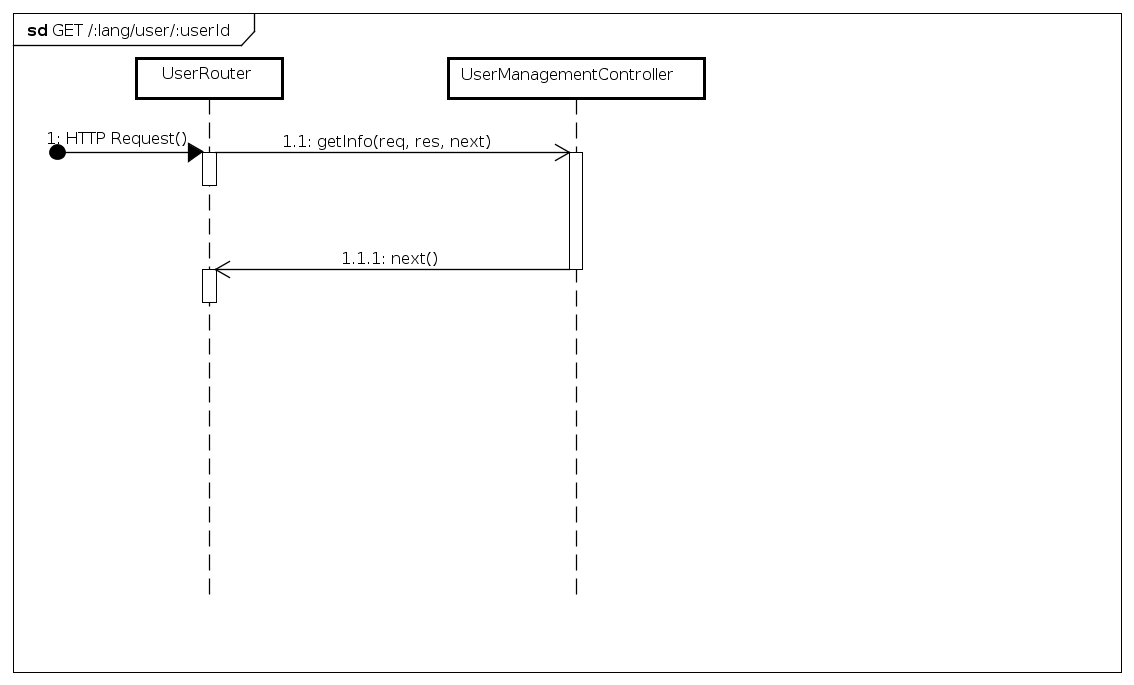
\includegraphics[scale=0.40]{UML/DiagrammiDiSequenza/Back-end/GET_LangUserUserIdSuccess.png}
	\caption{Procedura di visualizzazione dati utente}
\end{figure}

\FloatBarrier

\item \textbf{Fallimento}:
\\
Quando viene effettuata una richiesta di visualizzazione dei dati dell'utente sollevando un errore. Tale scenario rappresenta il fallimento di una richiesta di visualizzzione dei dati dell'utente che impone, come vincolo per poter essere effettuata, che l'utente sia autenticato al sistema. In questo caso il modulo \texttt{UserManagementController} invia \texttt{next(error)} per il fallimento di tale vincolo al router il quale avrà compito di reinstradarlo (indirizzandolo verso \texttt{ErrorHandler}).

\label{Fallimento della procedura di visualizzazione dati utente}
\begin{figure}[ht]
	\centering
	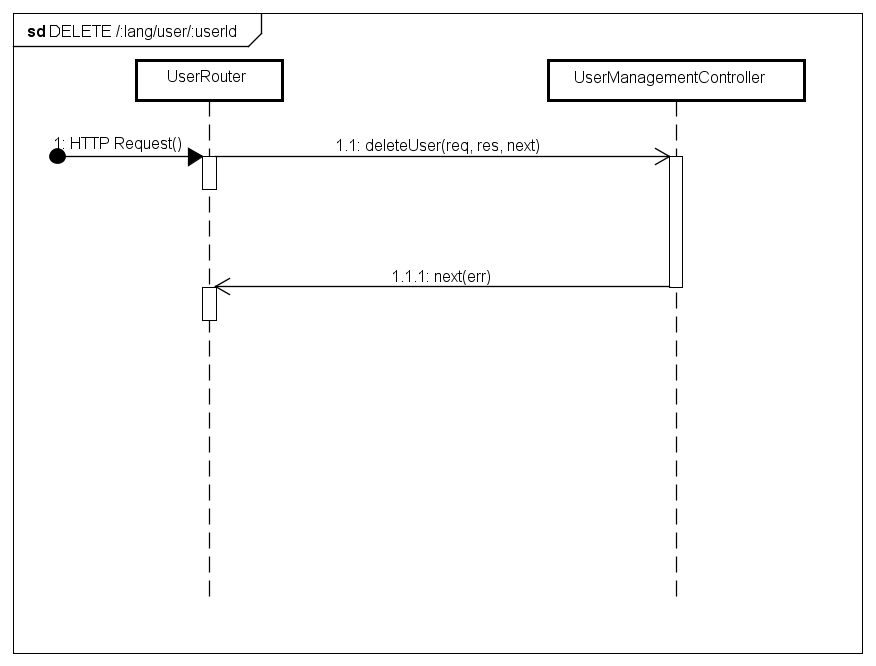
\includegraphics[scale=0.40]{UML/DiagrammiDiSequenza/Back-end/GET_LangUserUseridFailure.png}
	\caption{Fallimento della procedura di visualizzazione dati utente}
\end{figure}

\FloatBarrier
\end{itemize}

\paragraph{PUT /:lang/user/:userId}
\begin{itemize}
\item \textbf{Successo}:
\\
Questo scenario rappresenta il successo di una richiesta di modifica dei dati dell'utente che impone, come vincolo per poter essere effettuata, che l'utente sia autenticato al sistema.  
In questo caso il modulo \texttt{UserManagementController} invia \texttt{next()} al router per indicare il successo dell'operazione.
\label{Procedura di modifica dati utente}
\begin{figure}[ht]
	\centering
	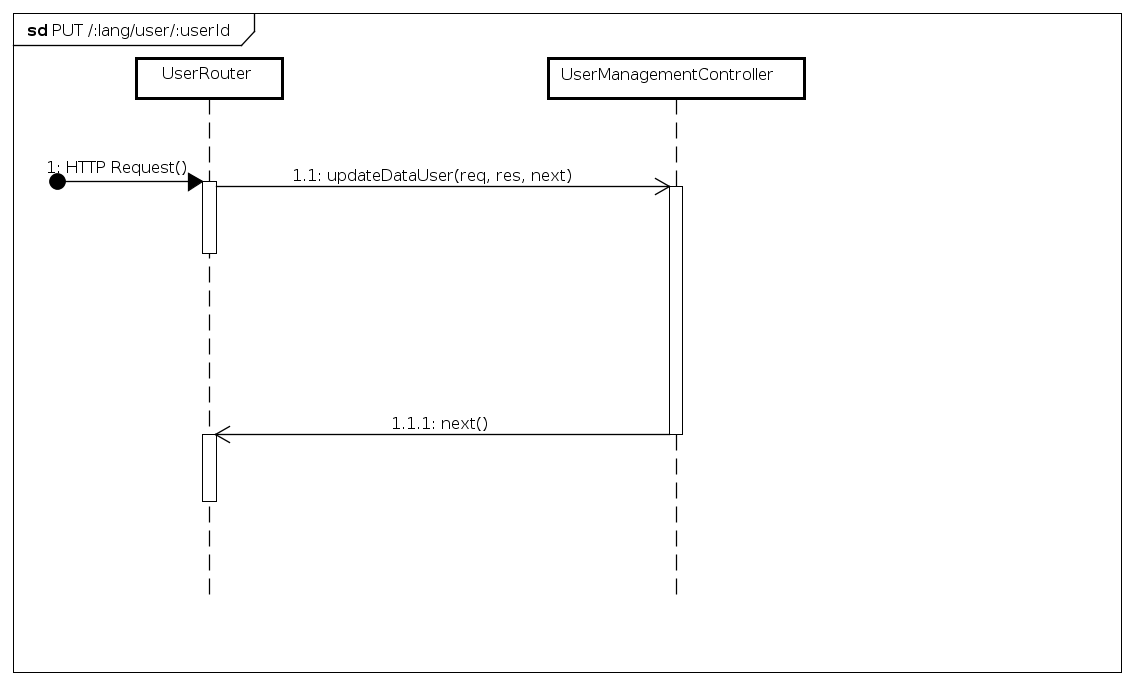
\includegraphics[scale=0.40]{UML/DiagrammiDiSequenza/Back-end/PUT_LangUserUseridSuccess.png}
	\caption{Procedura di modifica dati utente}
\end{figure}
\FloatBarrier

\item \textbf{Fallimento}:
\\
Quando viene effettuata una richiesta di modifica dei dati dell'utente sollevando un errore. Tale scenario rappresenta il fallimento di una richiesta di modifica dei dati dell'utente che impone, come vincolo per poter essere effettuata, che l'utente sia autenticato al sistema. In questo caso il modulo \texttt{UserManagementController} invia \texttt{next(error)} per il fallimento di tale vincolo al router il quale avrà compito di reinstradarlo (indirizzandolo verso \texttt{ErrorHandler}).
\label{Fallimento della procedura di modifica dati utente}
\begin{figure}[ht]
	\centering
	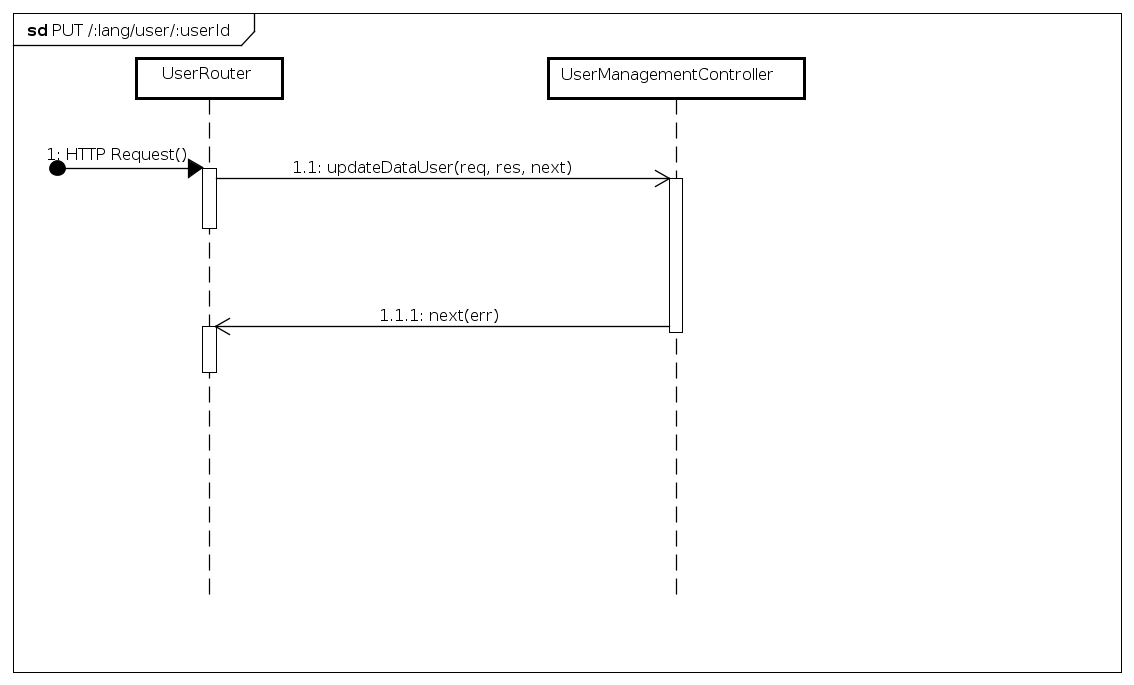
\includegraphics[scale=0.40]{UML/DiagrammiDiSequenza/Back-end/PUT_LangUserUseridFailure.png}
	
	\caption{Fallimento della procedura di modifica dati utente}
\end{figure}
\FloatBarrier
\end{itemize}

\paragraph{PUT /:lang/user/:userId/privacy}
\begin{itemize}
\item \textbf{Successo}:
\\
Questo scenario rappresenta il successo di una richiesta di modifica della passwprd dell'utente che impone, come vincolo per poter essere effettuata, che l'utente sia autenticato al sistema.  
In questo caso il modulo \texttt{UserManagementController} invia \texttt{next()} al router per indicare il successo dell'operazione.

\label{Procedura di modifica password}
\begin{figure}[ht]
	\centering
	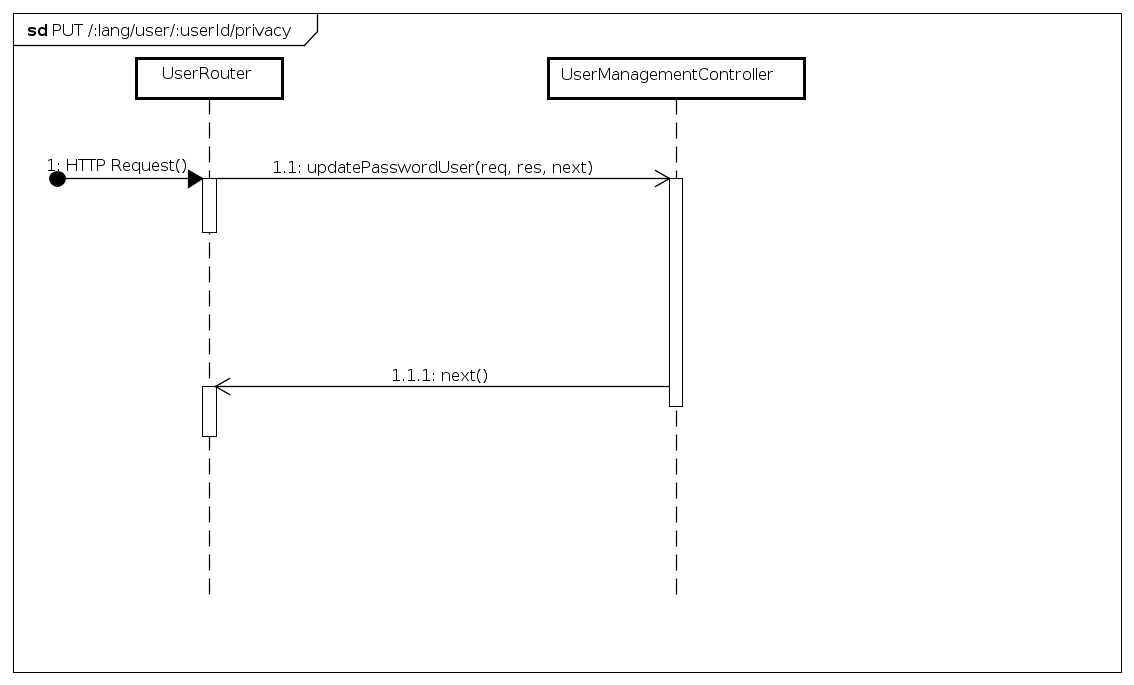
\includegraphics[scale=0.40]{UML/DiagrammiDiSequenza/Back-end/PUT_LangUserUserIdPrivacySuccess.png}
	\caption{Procedura di modifica password}
\end{figure}
\FloatBarrier
\item \textbf{Fallimento}:
\\
Quando viene effettuata una richiesta di modifica della password dell'utente sollevando un errore. Tale scenario rappresenta il fallimento di una richiesta di modifica della password dell'utente che impone, come vincolo per poter essere effettuata, che l'utente sia autenticato al sistema. In questo caso il modulo \texttt{UserManagementController} invia \texttt{next(error)} per il fallimento di tale vincolo al router il quale avrà compito di reinstradarlo (indirizzandolo verso \texttt{ErrorHandler}).



\label{Fallimento della procedura di modifica password}
\begin{figure}[ht]
	\centering
	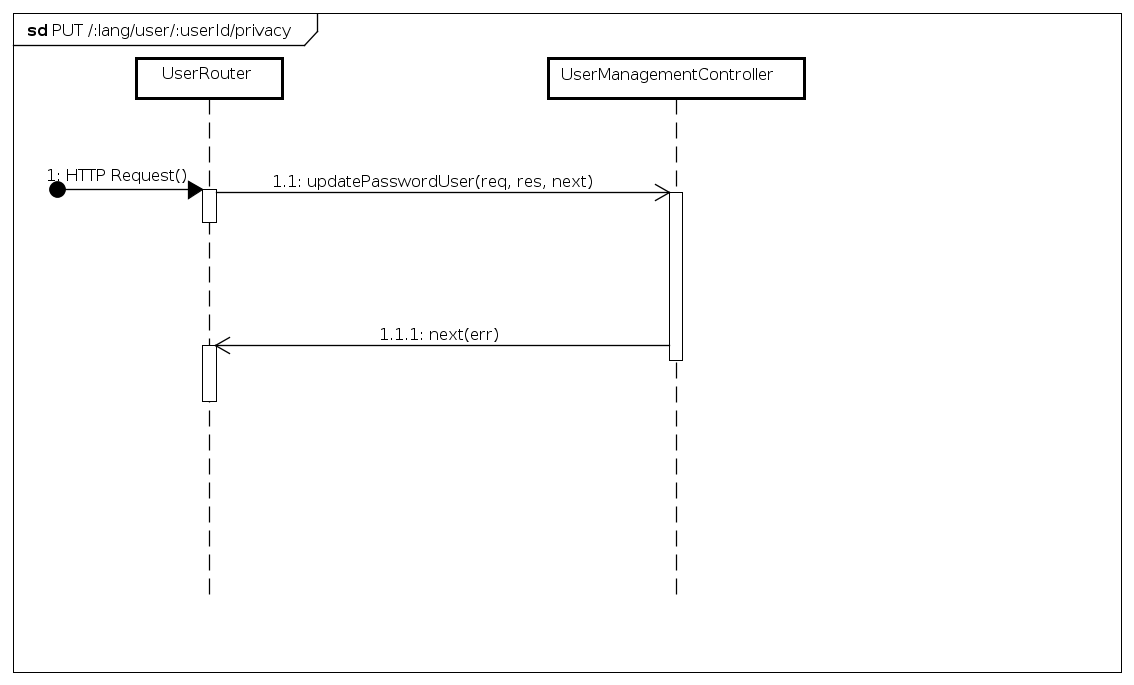
\includegraphics[scale=0.40]{UML/DiagrammiDiSequenza/Back-end/PUT_LangUserUserIdPrivacyFailure.png}	
	\caption{Fallimento della procedura di modifica password}
\end{figure}
\FloatBarrier
\end{itemize}


\paragraph{GET /:lang/user/:userId/statistics}
\begin{itemize}
\item \textbf{Successo}:
\\
Questo scenario rappresenta il successo di una richiesta di modifica delle statistiche  dell'utente che impone, come vincolo per poter essere effettuata, che l'utente sia autenticato al sistema.  
In questo caso il modulo \texttt{UserManagementController} invia \texttt{next()} al router per indicare il successo dell'operazione.

\label{Procedura di visualizzazione delle statistiche}
\begin{figure}[ht]
	\centering
	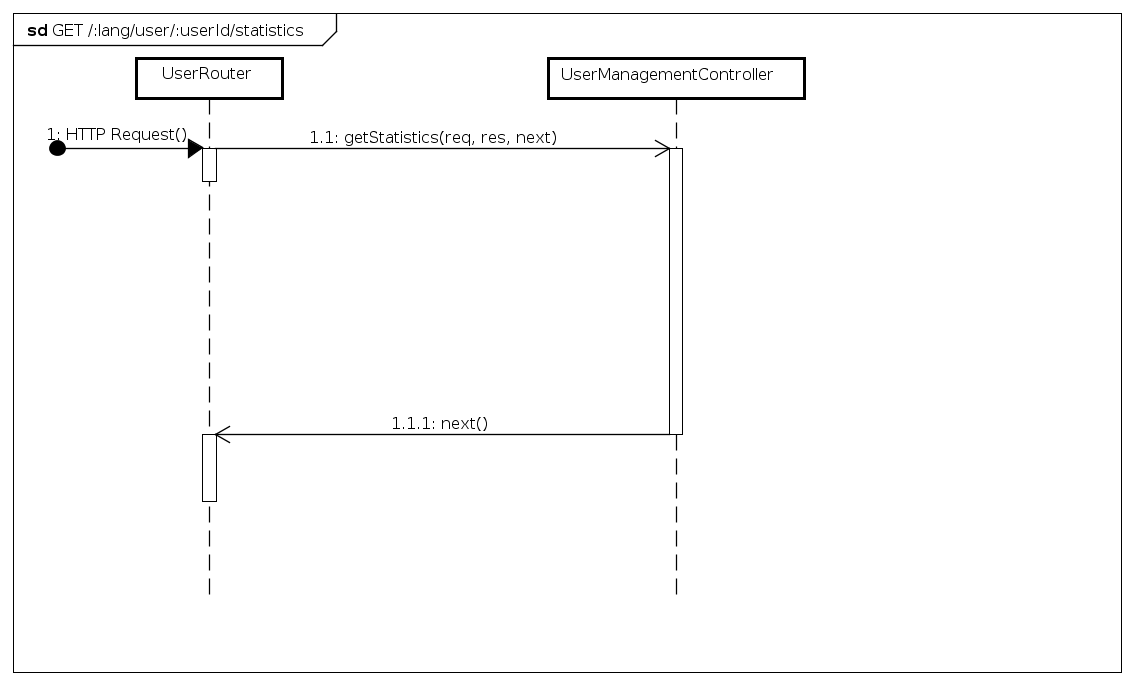
\includegraphics[scale=0.40]{UML/DiagrammiDiSequenza/Back-end/GET_LangUserUserIdStatisticsSuccess.png}
	\caption{Procedura di visualizzazione delle statistiche}
\end{figure}
\FloatBarrier
\item \textbf{Fallimento}:
\\
Quando viene effettuata una richiesta di visualizzazione delle statistiche dell'utente sollevando un errore. Tale scenario rappresenta il fallimento di una richiesta di visualizzazione delle statistiche dell'utente che impone, come vincolo per poter essere effettuata, che l'utente sia autenticato al sistema. In questo caso il modulo \texttt{UserManagementController} invia \texttt{next(error)} per il fallimento di tale vincolo al router il quale avrà compito di reinstradarlo (indirizzandolo verso \texttt{ErrorHandler}).

\label{Fallimento della procedura di visualizzazione delle statistiche}
\begin{figure}[ht]
	\centering
	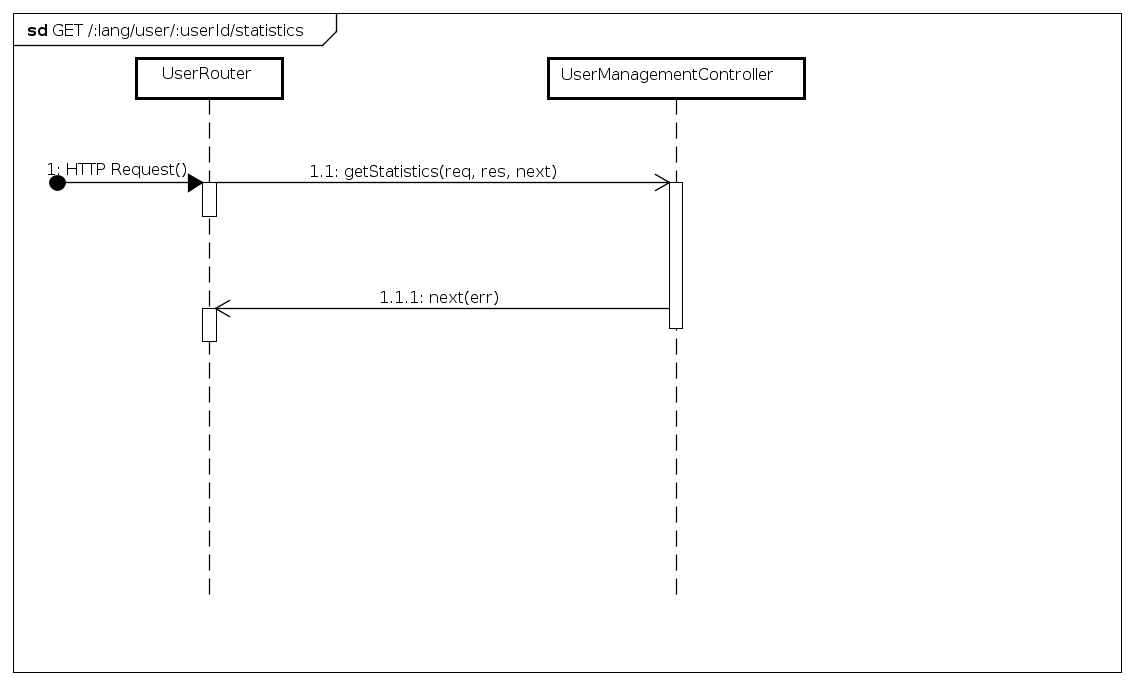
\includegraphics[scale=0.40]{UML/DiagrammiDiSequenza/Back-end/GET_LangUserUserIdStatisticsFailure.png}
	\caption{Fallimento della procedura di visualizzazione delle statistiche}
\end{figure}
\FloatBarrier
\end{itemize}

\paragraph{GET /:lang/user/:userId/statistics/summary/}
\begin{itemize}
\item \textbf{Successo}:
\\
Questo scenario rappresenta il successo di una richiesta di visualizzazione della cronologia dei questionari svolti dall'utente che impone, come vincolo per poter essere effettuata, che l'utente sia autenticato al sistema.  
In questo caso il modulo \texttt{UserManagementController} invia \texttt{next()} al router per indicare il successo dell'operazione.
\label{Procedura di visualizzazione della cronologia dei questionari svolti}
\begin{figure}[ht]
	\centering
	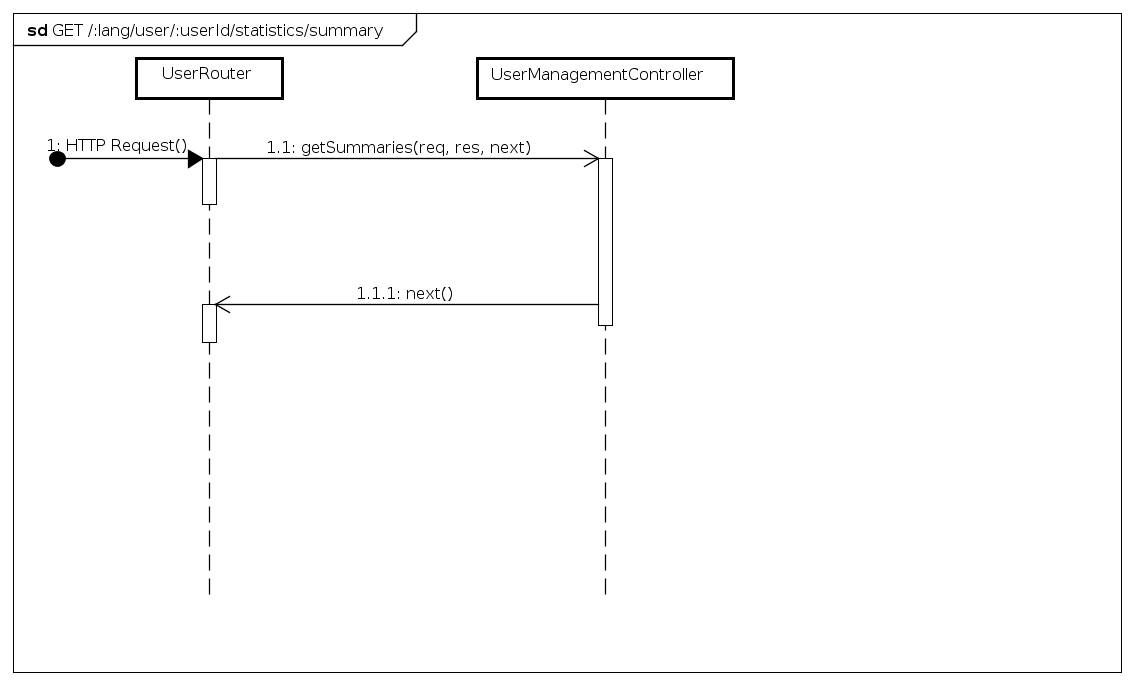
\includegraphics[scale=0.40]{UML/DiagrammiDiSequenza/Back-end/GET_LangUserUserIdStatisticsSummarySuccess.png}
	\caption{Procedura di visualizzazione della cronologia dei questionari svolti}
\end{figure}
\FloatBarrier
\item \textbf{Fallimento}:
\\
Quando viene effettuata una richiesta di visualizzazione della cronologia dei questionari svolti dall'utente sollevando un errore. Tale scenario rappresenta il fallimento di una richiesta di visualizzazione della cronologia dei questionari svolti dall'utente che impone, come vincolo per poter essere effettuata, che l'utente sia autenticato al sistema. In questo caso il modulo \texttt{UserManagementController} invia \texttt{next(error)} per il fallimento di tale vincolo al router il quale avrà compito di reinstradarlo (indirizzandolo verso \texttt{ErrorHandler}).
\label{Fallimento della procedura di visualizzazione della cronologia dei questionari svolti}
\begin{figure}[ht]
	\centering
	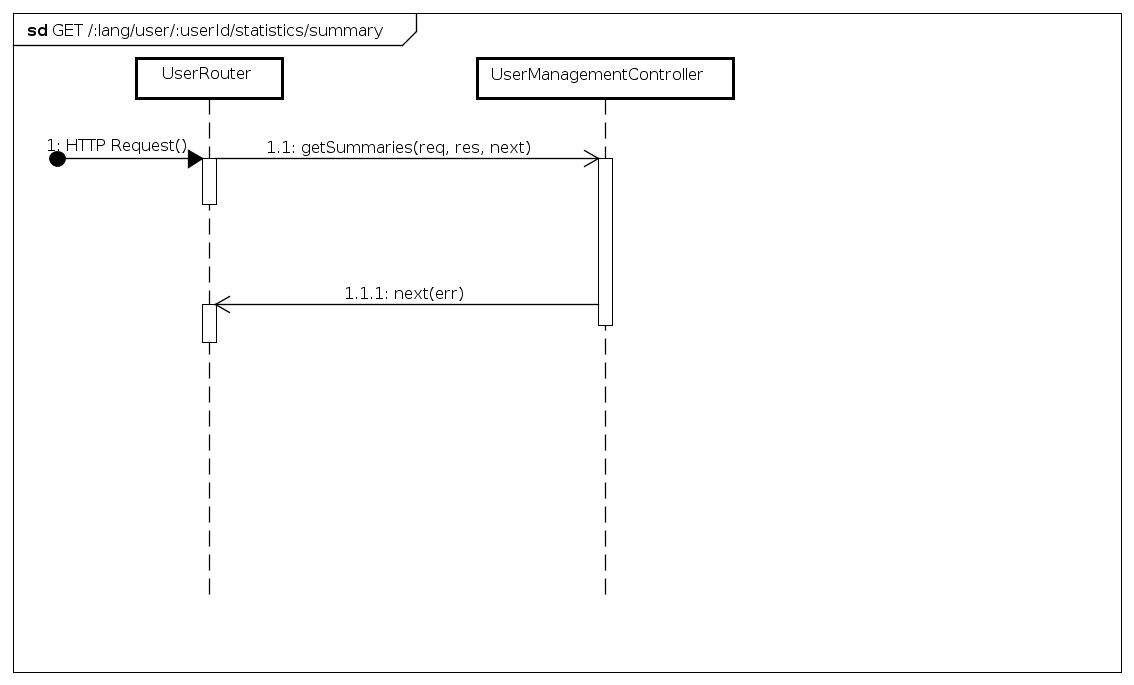
\includegraphics[scale=0.40]{UML/DiagrammiDiSequenza/Back-end/GET_LangUserUserIdStatisticsSummaryFailure.png}
	\caption{Fallimento della procedura di visualizzazione della cronologia dei questionari svolti}
\end{figure}
\FloatBarrier

\end{itemize}

\paragraph{GET /:lang/user/:userId/statistics/summary/:summaryId}
\begin{itemize}
\item \textbf{Successo}:
\\
Questo scenario rappresenta il successo di una richiesta di visualizzazione del riepilogo di un particolare questionario svolto dall'utente che impone, come vincolo per poter essere effettuata, che l'utente sia autenticato al sistema.  
In questo caso il modulo \texttt{UserManagementController} invia \texttt{next()} al router per indicare il successo dell'operazione.
\label{Procedura di visualizzazione del riepilogo di un particolare questionario svolto}
\begin{figure}[ht]
	\centering
	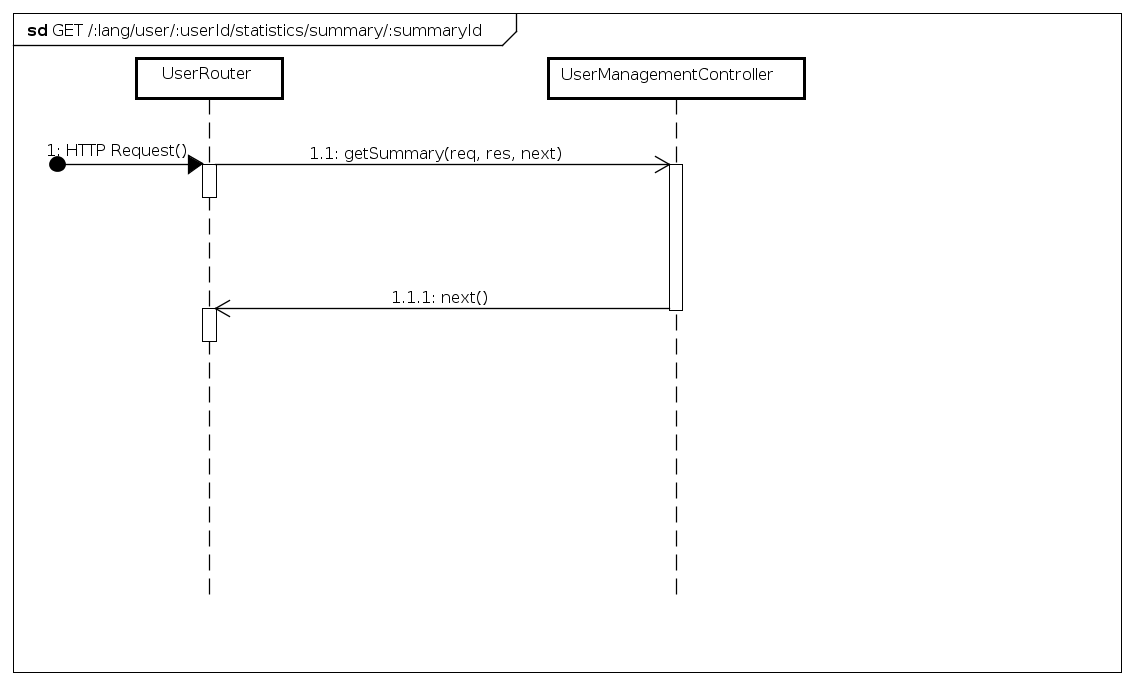
\includegraphics[scale=0.40]{UML/DiagrammiDiSequenza/Back-end/GET_LangUserUserIdStatisticsSummarySummaryIdSuccess.png}
	\caption{Procedura di visualizzazione del riepilogo di un particolare questionario svolto}
\end{figure}
\FloatBarrier
\item \textbf{Fallimento}:
\\
Quando viene effettuata una richiesta di visualizzazione del riepilogo di un particolare questionario svolto dall'utente sollevando un errore. Tale scenario rappresenta il fallimento di una richiesta di visualizzazione del riepilogo di un particolare questionario svolto dall'utente che impone, come vincolo per poter essere effettuata, che l'utente sia autenticato al sistema. In questo caso il modulo \texttt{UserManagementController} invia \texttt{next(error)} per il fallimento di tale vincolo al router il quale avrà compito di reinstradarlo (indirizzandolo verso \texttt{ErrorHandler}).
\label{Fallimento della procedura di visualizzazione del riepilogo di un particolare questionario svolto}
\begin{figure}[ht]
	\centering
	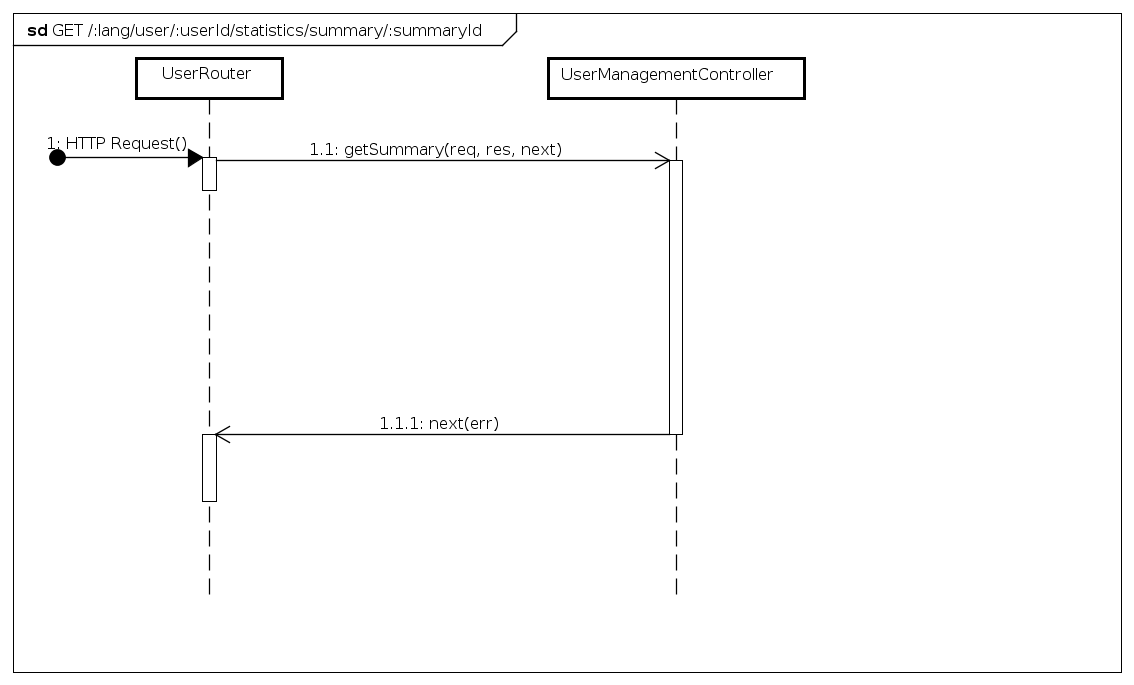
\includegraphics[scale=0.40]{UML/DiagrammiDiSequenza/Back-end/GET_LangUserUserIdStatisticsSummarySummaryIdFailure.png}
	\caption{Fallimento della procedura di visualizzazione del riepilogo di un particolare questionario svolto}
\end{figure}
\FloatBarrier
\end{itemize}




\paragraph{GET /:lang/user/:userId/quiz} % Restituisce i questionari creati dall'utente pro
\begin{itemize}
\item \textbf{Successo}:\\
Questo scenario rappresenta il successo di una richiesta di visualizzazione dei questionari creati che impone, come vincolo per poter essere effettuata, che l'utente sia autenticato al sistema e sia un utente pro. In questo caso il modulo \texttt{QuizController} invia \texttt{next()} per indicare il successo dell'operazione.
\label{Procedura di visualizzazione questionari creati}
\begin{figure}[ht]
	\centering
	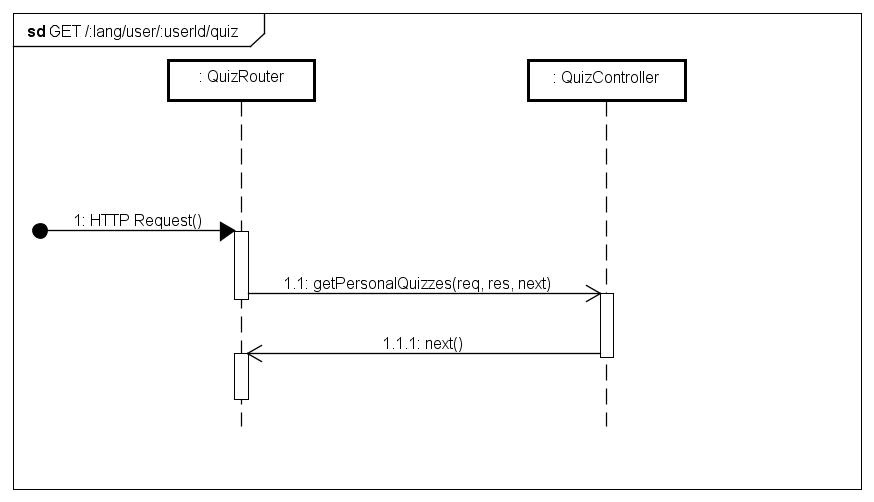
\includegraphics[scale=0.40]{UML/DiagrammiDiSequenza/Back-end/GET__lang_user_userId_quiz_success.png}
	\caption{Procedura di visualizzazione questionari creati}
\end{figure}
\FloatBarrier

\item \textbf{Fallimento}:\\
Questo scenario rappresenta il fallimento di una richiesta di visualizzazione dei questionari creati che impone, come vincolo per poter essere effettuata, che l'utente sia autenticato al sistema e sia un utente pro. In questo caso il modulo \texttt{QuizController} invia \texttt{next(error)} per indicare il fallimento di tale vincolo al router il quale avrà compito di reinstradarlo (indirizzandolo verso \texttt{ErrorHandler}).
\label{Fallimento della procedura di visualizzazione questionari creati}
\begin{figure}[ht]
	\centering
	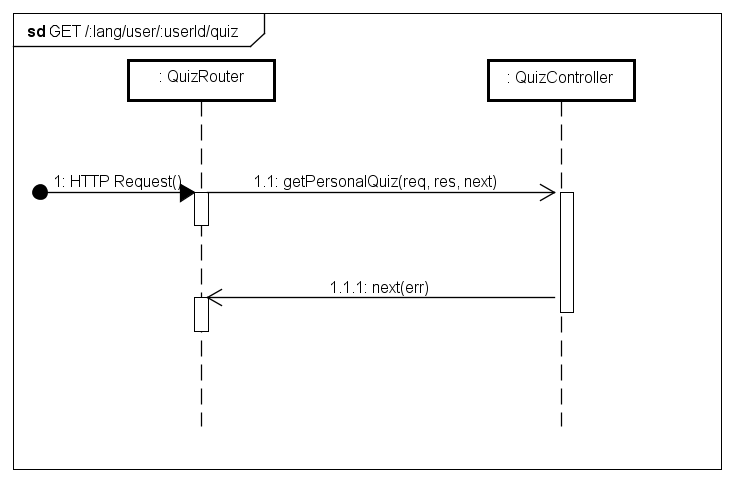
\includegraphics[scale=0.40]{UML/DiagrammiDiSequenza/Back-end/GET__lang_user_userId_quiz_failure.png}
	\caption{Fallimento della procedura di visualizzazione questionari creati}
\end{figure}
\FloatBarrier
\end{itemize}

\paragraph{POST /:lang/user/:useId/quiz} % Aggiunge un questionario nel sistema, restituisce un messaggio di conferma o di errore
\begin{itemize}
\item \textbf{Successo}:\\
Questo scenario rappresenta il successo di una richiesta di creazione di un questionario che impone, come vincolo per poter essere effettuata, che l'utente sia autenticato al sistema e sia un utente pro. In questo caso il modulo \texttt{QuizController} invia \texttt{next()} per indicare il successo dell'operazione.
\label{Procedura di creazione di un questionario}
\begin{figure}[ht]
	\centering
	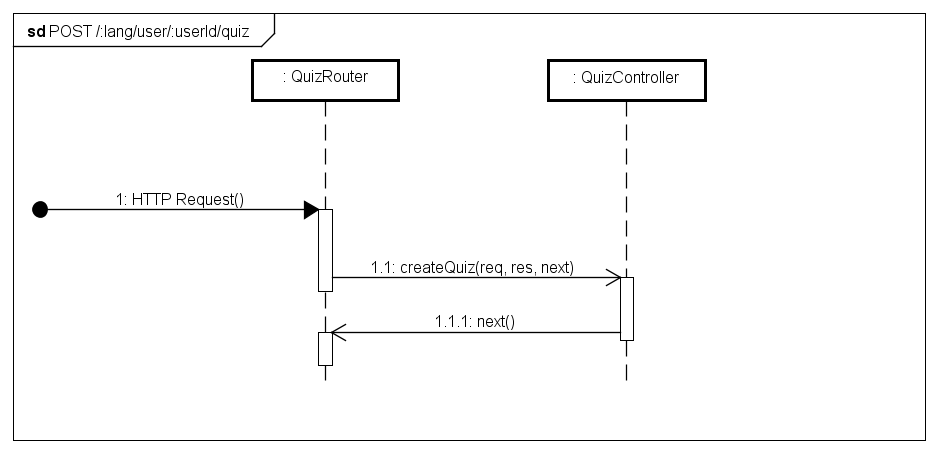
\includegraphics[scale=0.40]{UML/DiagrammiDiSequenza/Back-end/POST__lang_user_userId_quiz_success.png}
	\caption{Procedura di creazione di un questionario}
\end{figure}
\FloatBarrier

\item \textbf{Fallimento}:\\
Questo scenario rappresenta il fallimento di una richiesta di creazione di un questionario che impone, come vincolo per poter essere effettuata, che l'utente sia autenticato al sistema e sia un utente pro. In questo caso il modulo \texttt{QuizController} invia \texttt{next(error)} per indicare il fallimento di tale vincolo al router il quale avrà compito di reinstradarlo (indirizzandolo verso \texttt{ErrorHandler}).
\label{Fallimento della procedura di creazione di un questionario}
\begin{figure}[ht]
	\centering
	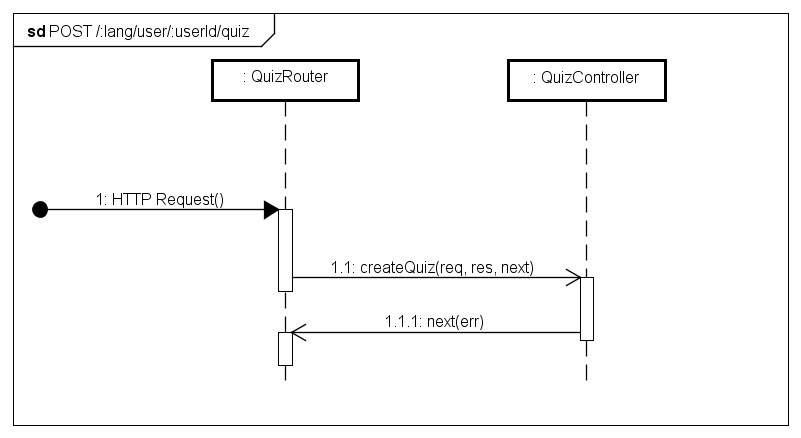
\includegraphics[scale=0.40]{UML/DiagrammiDiSequenza/Back-end/POST__lang_user_userId_quiz_failure.png}
	\caption{Fallimento della procedura di creazione di un questionario}
\end{figure}
\FloatBarrier
\end{itemize}

\paragraph{POST /:lang/user/:userId/quiz/:quizId/addUser} % Iscrive un utente ad un questionario, restituisce un messaggio di conferma o di errore
\begin{itemize}
\item \textbf{Successo}:\\
Questo scenario rappresenta il successo di una richiesta di iscrizione ad un questionario che impone, come vincolo per poter essere effettuata, che l'utente sia autenticato al sistema. In questo caso il modulo \texttt{QuizController} invia \texttt{next()} per indicare il successo dell'operazione.
\label{Procedura di iscrizione ad un questionario}
\begin{figure}[ht]
	\centering
	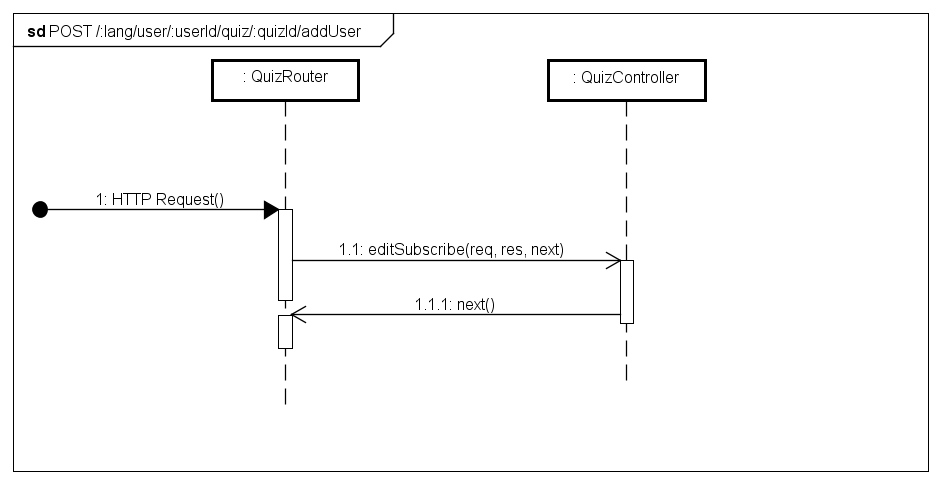
\includegraphics[scale=0.40]{UML/DiagrammiDiSequenza/Back-end/POST__lang_user_userId_quiz_quizId_addUser_success.png}
	\caption{Procedura di iscrizione ad un questionario}
\end{figure}
\FloatBarrier

\item \textbf{Fallimento}:\\
Questo scenario rappresenta il fallimento di una richiesta di iscrizione ad un questionario che impone, come vincolo per poter essere effettuata, che l'utente sia autenticato al sistema. In questo caso il modulo \texttt{QuizController} invia \texttt{next(error)} per indicare il fallimento di tale vincolo al router il quale avrà compito di reinstradarlo (indirizzandolo verso \texttt{ErrorHandler}).
\label{Fallimento della procedura di iscrizione ad un questionario}
\begin{figure}[ht]
	\centering
	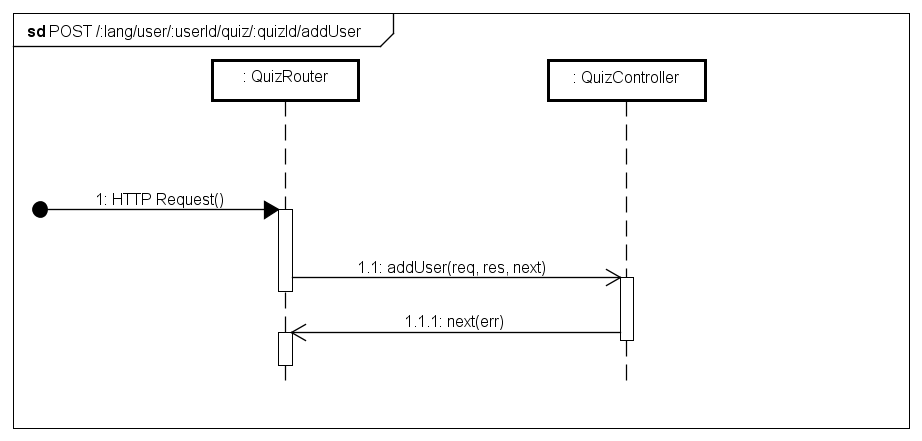
\includegraphics[scale=0.40]{UML/DiagrammiDiSequenza/Back-end/POST__lang_user_userId_quiz_quizId_addUser_failure.png}
	\caption{Fallimento della procedura di iscrizione ad un questionario}
\end{figure}
\FloatBarrier
\end{itemize}

\paragraph{POST /:lang/user/:userId/quiz/:quizId/activeUser} % Aggiunge un utente iscritto al questionario nella lista degli utenti che lo hanno eseguito
\begin{itemize}
\item \textbf{Successo}:\\
Questo scenario rappresenta il successo di una richiesta di aggiunta alla lista di utenti che hanno compilato un questionario che impone, come vincolo per poter essere effettuata, che l'utente sia autenticato al sistema. In questo caso il modulo \texttt{QuizController} invia \texttt{next()} per indicare il successo dell'operazione.
\label{Procedura di aggiunta alla lista di utenti che hanno compilato un questionario}
\begin{figure}[ht]
	\centering
	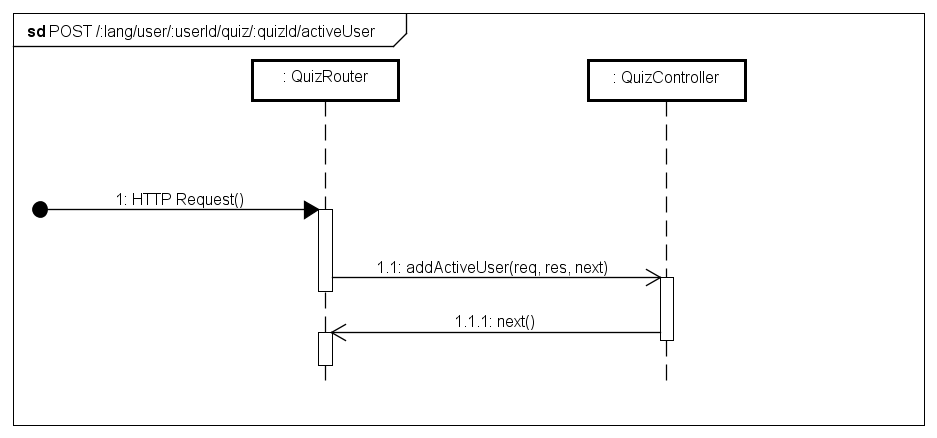
\includegraphics[scale=0.40]{UML/DiagrammiDiSequenza/Back-end/POST__lang_user_userId_quiz_quizId_activeUser_success.png}
	\caption{Procedura di aggiunta alla lista di utenti che hanno compilato un questionario}
\end{figure}
\FloatBarrier

\item \textbf{Fallimento}:\\
Questo scenario rappresenta il fallimento di una richiesta di aggiunta alla lista di utenti che hanno compilato un questionario che impone, come vincolo per poter essere effettuata, che l'utente sia autenticato al sistema. In questo caso il modulo \texttt{QuizController} invia \texttt{next(error)} per indicare il fallimento di tale vincolo al router il quale avrà compito di reinstradarlo (indirizzandolo verso \texttt{ErrorHandler}).
\label{Fallimento della procedura di aggiunta alla lista di utenti che hanno compilato un questionario}
\begin{figure}[ht]
	\centering
	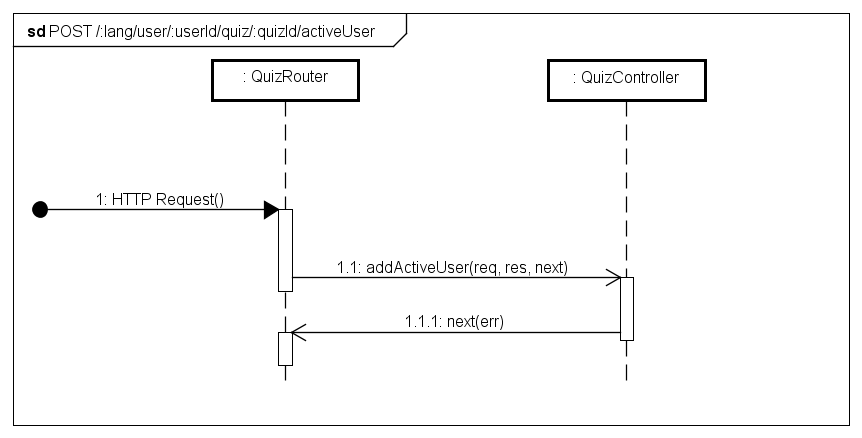
\includegraphics[scale=0.40]{UML/DiagrammiDiSequenza/Back-end/POST__lang_user_userId_quiz_quizId_activeUser_failure.png}
	\caption{Fallimento della procedura di aggiunta alla lista di utenti che hanno compilato un questionario}
\end{figure}
\FloatBarrier
\end{itemize}

\paragraph{PUT /:lang/user/:userId/quiz/:quizId} % Modifica di un questionario creato in precedenza, restituisce un messaggio di conferma o di errore
\begin{itemize}
\item \textbf{Successo}:\\
Questo scenario rappresenta il successo di una richiesta di modifica di un questionario che impone, come vincolo per poter essere effettuata, che l'utente sia autenticato al sistema e sia l'utente pro che aveva creato il questionario che si vuole modificare. In questo caso il modulo \texttt{QuizController} invia \texttt{next()} per indicare il successo dell'operazione.
\label{Procedura di modifica di un questionario}
\begin{figure}[ht]
	\centering
	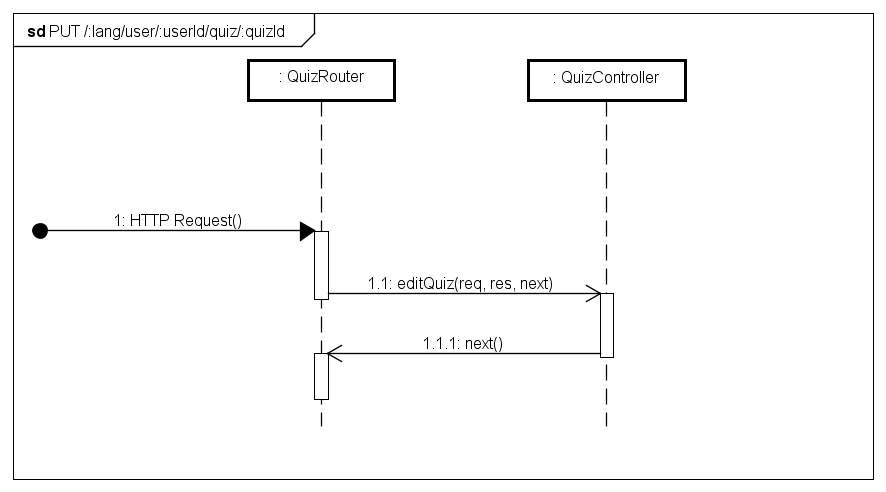
\includegraphics[scale=0.40]{UML/DiagrammiDiSequenza/Back-end/PUT__lang_user_userId_quiz_quizId_success.png}
	\caption{Procedura di modifica di un questionario}
\end{figure}
\FloatBarrier

\item \textbf{Fallimento}:\\
Questo scenario rappresenta il fallimento di una richiesta di modifica di un questionario che impone, come vincolo per poter essere effettuata, che l'utente sia autenticato al sistema e sia l'utente pro che aveva creato il questionario che si vuole modificare. In questo caso il modulo \texttt{QuizController} invia \texttt{next(error)} per indicare il fallimento di tale vincolo al router il quale avrà compito di reinstradarlo (indirizzandolo verso \texttt{ErrorHandler}).
\label{Fallimento della procedura di modifica di un questionario}
\begin{figure}[ht]
	\centering
	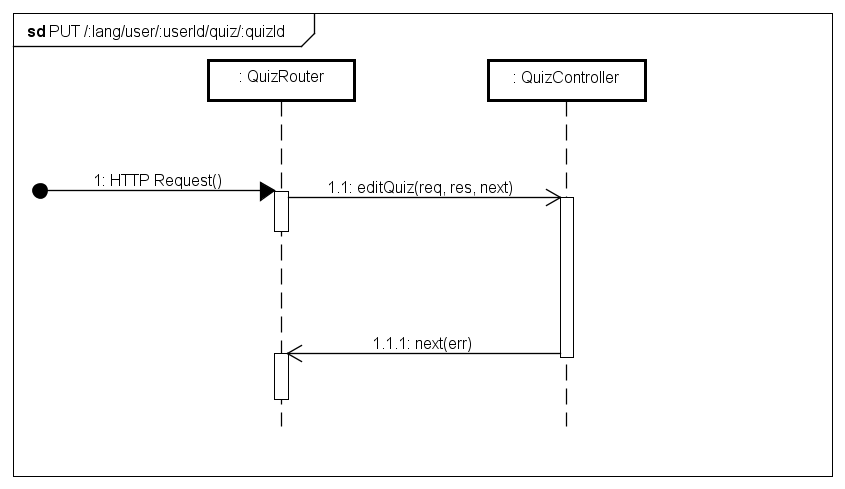
\includegraphics[scale=0.40]{UML/DiagrammiDiSequenza/Back-end/PUT__lang_user_userId_quiz_quizId_failure.png}
	\caption{Fallimento della procedura di modifica di un questionario}
\end{figure}
\FloatBarrier
\end{itemize}

\paragraph{GET /:lang/user/:userId/quiz/:quizId/test} % Restituisce il quiz selezionato dall'utente per effettuare l'esercitazione
\begin{itemize}
\item \textbf{Successo}:\\
Questo scenario rappresenta il successo di una richiesta di visualizzazione del questionario da compilare che impone, come vincolo per poter essere effettuata, che l'utente sia autenticato al sistema e che sia iscritto e in seguito abilitato a compilare il questionario. In questo caso il modulo \texttt{QuizController} invia \texttt{next()} per indicare il successo dell'operazione.
\label{Procedura di visualizzazione del questionario da compilare}
\begin{figure}[ht]
	\centering
	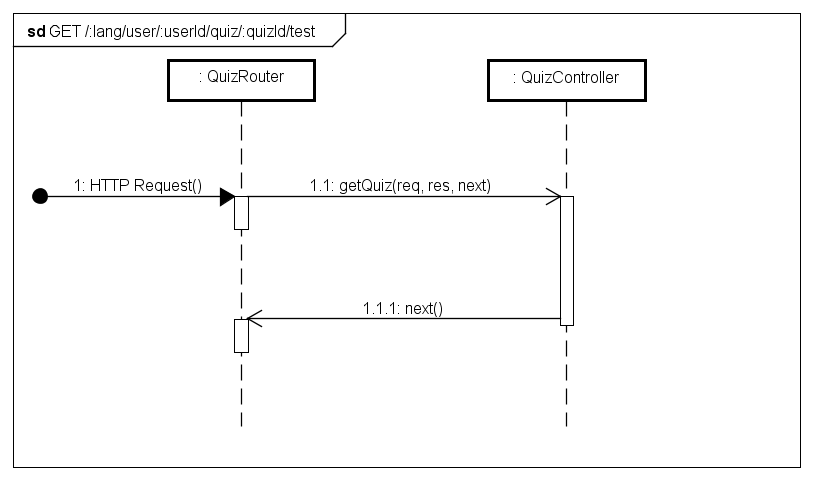
\includegraphics[scale=0.40]{UML/DiagrammiDiSequenza/Back-end/GET__lang_user_userId_quiz_quizId_test_success.png}
	\caption{Procedura di visualizzazione del questionario da compilare}
\end{figure}
\FloatBarrier

\item \textbf{Fallimento}:\\
Questo scenario rappresenta il fallimento di una richiesta di visualizzazione del questionario da compilare che impone, come vincolo per poter essere effettuata, che l'utente sia autenticato al sistema e che sia iscritto e in seguito abilitato a compilare il questionario. In questo caso il modulo \texttt{QuizController} invia \texttt{next(error)} per indicare il fallimento di tale vincolo al router il quale avrà compito di reinstradarlo (indirizzandolo verso \texttt{ErrorHandler}).
\label{Fallimento della procedura di visualizzazione del questionario da compilare}
\begin{figure}[ht]
	\centering
	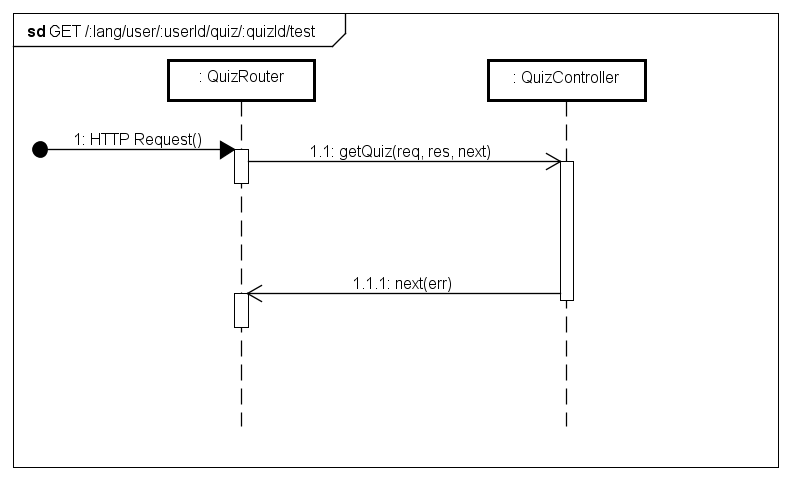
\includegraphics[scale=0.40]{UML/DiagrammiDiSequenza/Back-end/GET__lang_user_userId_quiz_quizId_test_failure.png}
	\caption{Fallimento della procedura di visualizzazione del questionario da compilare}
\end{figure}
\FloatBarrier
\end{itemize}

\paragraph{POST /:lang/user/:userId/quiz/:quizId/summary} % Crea il riepilogo del questionario svolto;
\begin{itemize}
\item \textbf{Successo}:\\
Questo scenario rappresenta il successo di una richiesta di creazione di un riepilogo che impone, come vincolo per poter essere effettuata, che l'utente sia autenticato al sistema e che abbia finito di compilare un questionario. In questo caso il modulo \texttt{SummaryController} invia \texttt{next()} per indicare il successo dell'operazione e successivamente verrà effettuata la updateSummary() per aggiornare la cronologia dell'utente.
\label{Procedura di creazione di un riepilogo}
\begin{figure}[ht]
	\centering
	\includegraphics[scale=0.40]{UML/DiagrammiDiSequenza/Back-end/POST__lang_user_userId_quiz_quizId_summary_success.png}
	\caption{Procedura di creazione di un riepilogo}
\end{figure}
\FloatBarrier

\item \textbf{Fallimento}:\\
Questo scenario rappresenta il fallimento di una richiesta di creazione di un riepilogo che impone, come vincolo per poter essere effettuata, che l'utente sia autenticato al sistema e che abbia finito di compilare un questionario. In questo caso il modulo \texttt{SummaryController} invia \texttt{next(error)} per indicare il fallimento di tale vincolo al router il quale avrà compito di reinstradarlo (indirizzandolo verso \texttt{ErrorHandler}).
\label{Fallimento della procedura di creazione di un riepilogo}
\begin{figure}[ht]
	\centering
	\includegraphics[scale=0.40]{UML/DiagrammiDiSequenza/Back-end/POST__lang_user_userId_quiz_quizId_summary_failure.png}
	\caption{Fallimento della procedura di creazione di un riepilogo}
\end{figure}
\FloatBarrier
\end{itemize}



\paragraph{GET /:lang/user/:userId/question}
\begin{itemize}
\item \textbf{Successo}
% descrizione diagramma e UML

\textbf{Descrizione}: il \texttt{QuestionRouter} gestisce la richiesta \textit{REST\ped{G}} del Front-End passando il controllo al \texttt{QuestionController}; viene poi invocato il metodo\\ \texttt{getQuestions(req,res,next)} che ritorna tutte le domande create dall'utente.

\begin{figure}[ht]
	\centering
	\includegraphics[scale=0.45]{UML/DiagrammiDiSequenza/Back-end/GET__lang_user__userId_question.png}
	\caption{GET /:lang/user/:userId/question}
\end{figure}
\FloatBarrier

\item \textbf{Fallimento}
% descrizione diagramma e UML
\end{itemize}

\paragraph{POST /:lang/user/question}
\begin{itemize}
\item \textbf{Successo}
% descrizione diagramma e UML

\textbf{Descrizione}: il \texttt{QuestionRouter} gestisce la richiesta \textit{REST\ped{G}} del Front-End passando il controllo al \texttt{QuestionController}; viene poi invocato il metodo\\ \texttt{createQuestion(req,res,next)} che inserisce una nuova domanda creata all'interno del sistema.

\begin{figure}[ht]
	\centering
	\includegraphics[scale=0.45]{UML/DiagrammiDiSequenza/Back-end/POST__lang_user_question.png}
	\caption{POST /:lang/user/question}
\end{figure}
\FloatBarrier

\item \textbf{Fallimento}
% descrizione diagramma e UML
\end{itemize}

\paragraph{GET /:lang/user/:userId/search/:keyword/users}
\begin{itemize}
\item \textbf{Successo}: questo scenario rappresenta il successo di una richiesta che ritorna la lista degli utenti il cui username contiene la keyword inserita nella barra di ricerca che impone, come vincolo per poter essere effettuata, che l'utente sia autenticato al sistema; quindi prima di tale operazione deve venire fatta una richiesta di controllo di sessione mediante l'apposita \textit{REST\ped{G}}. In questo caso il modulo \texttt{UserManagementController} invia \texttt{next()} per indicare il successo dell'operazione.

\begin{figure}[ht]
	\centering
	\includegraphics[scale=0.45]{UML/DiagrammiDiSequenza/Back-end/GET__lang_user__userId_search__keyword_users_success.png}
	\caption{Procedura di visualizzazione dei risultati della ricerca utente}
\end{figure}
\FloatBarrier

\item \textbf{Fallimento}: questo scenario rappresenta il fallimento di una richiesta che ritorna la lista degli utenti il cui username contiene la keyword inserita nella barra di ricerca che impone, come vincolo per poter essere effettuata, che l'utente sia autenticato al sistema; quindi prima di tale operazione deve venire fatta una richiesta di controllo di sessione mediante l'apposita \textit{REST\ped{G}}. In questo caso il modulo \texttt{UserManagementController} invia \texttt{next(error)} per indicare il fallimento di tale vincolo al router il quale avrà compito di reinstradarlo (indirizzandolo verso \texttt{ErrorHandler}).

\begin{figure}[ht]
	\centering
	\includegraphics[scale=0.45]{UML/DiagrammiDiSequenza/Back-end/GET__lang_user__userId_search__keyword_users_failure.png}
	\caption{Fallimento della procedura di visualizzazione dei risultati della ricerca utente}
\end{figure}
\FloatBarrier

\end{itemize}

\paragraph{GET /:lang/user/:userId/search/:keyword/quizzes}
\begin{itemize}
\item \textbf{Successo}: questo scenario rappresenta il successo di una richiesta che ritorna la lista dei questionari il cui titolo contiene la keyword inserita nella barra di ricerca che impone, come vincolo per poter essere effettuata, che l'utente sia autenticato al sistema; quindi prima di tale operazione deve venire fatta una richiesta di controllo di sessione mediante l'apposita \textit{REST\ped{G}}. In questo caso il modulo \texttt{QuizController} invia \texttt{next()} per indicare il successo dell'operazione.

\begin{figure}[ht]
	\centering
	\includegraphics[scale=0.45]{UML/DiagrammiDiSequenza/Back-end/GET__lang_user__userId_search__keyword_quizzes_success.png}
	\caption{Procedura di visualizzazione dei risultati della ricerca questionario}
\end{figure}
\FloatBarrier

\item \textbf{Fallimento}: questo scenario rappresenta il fallimento di una richiesta che ritorna la lista dei questionari il cui titolo contiene la keyword inserita nella barra di ricerca che impone, come vincolo per poter essere effettuata, che l'utente sia autenticato al sistema; quindi prima di tale operazione deve venire fatta una richiesta di controllo di sessione mediante l'apposita \textit{REST\ped{G}}. In questo caso il modulo \texttt{QuizController} ritornerà un \texttt{next(error)} al router che avrà il compito di reinstradarlo (indirizzandolo verso \texttt{ErrorHandler}).

\begin{figure}[ht]
	\centering
	\includegraphics[scale=0.45]{UML/DiagrammiDiSequenza/Back-end/GET__lang_user__userId_search__keyword_quizzes_failure.png}
	\caption{Fallimento della procedura di visualizzazione dei risultati della ricerca questionario}
\end{figure}
\FloatBarrier
\end{itemize}






\paragraph{GET /:lang/user/:userId/search/users/:users}
\begin{itemize}
\item \textbf{Successo}: questo scenario rappresenta il successo di una richiesta di visualizzazione di un utente tra quelli ritornati come risultato della ricerca che impone, come vincolo per poter essere effettuata, che l'utente sia autenticato al sistema; quindi prima di tale operazione deve venire fatta una richiesta di controllo di sessione mediante l'apposita \textit{REST\ped{G}}. In questo caso il modulo \texttt{UserManagementController} invia \texttt{next()} per indicare il successo dell'operazione.

\begin{figure}[ht]
	\centering
	\includegraphics[scale=0.45]{UML/DiagrammiDiSequenza/Back-end/GET__lang_user__userId_search_users__users_success.png}
	\caption{Procedura di visualizzazione di un utente}
\end{figure}
\FloatBarrier

\item \textbf{Fallimento}: questo scenario rappresenta il fallimento di una richiesta di visualizzazione di un utente tra quelli ritornati come risultato della ricerca che impone, come vincolo per poter essere effettuata, che l'utente sia autenticato al sistema; quindi prima di tale operazione deve venire fatta una richiesta di controllo di sessione mediante l'apposita \textit{REST\ped{G}}. In questo caso il modulo \texttt{UserManagementController} invia \texttt{next(error)} per indicare il fallimento di tale vincolo al router il quale avrà compito di reinstradarlo (indirizzandolo verso \texttt{ErrorHandler}).

\begin{figure}[ht]
	\centering
	\includegraphics[scale=0.45]{UML/DiagrammiDiSequenza/Back-end/GET__lang_user__userId_search_users__users_failure.png}
	\caption{Fallimento della procedura della visualizzazione di un utente}
\end{figure}
\FloatBarrier

\end{itemize}





\paragraph{GET /:lang/user/:userId/search/quizzes/:quizId}
\begin{itemize}
\item \textbf{Successo}: questo scenario rappresenta il successo di una richiesta di visualizzazione di un questionario tra quelli ritornati come risultato della ricerca che impone, come vincolo per poter essere effettuata, che l'utente sia autenticato al sistema; quindi prima di tale operazione deve venire fatta una richiesta di controllo di sessione mediante l'apposita \textit{REST\ped{G}}. In questo caso il modulo \texttt{QuizController} invia \texttt{next()} per indicare il successo dell'operazione.

\begin{figure}[ht]
	\centering
	\includegraphics[scale=0.45]{UML/DiagrammiDiSequenza/Back-end/GET__lang_user__userId_search_quizzes__quizId_success.png}
	\caption{Procedura della visualizzazione di un questionario}
\end{figure}
\FloatBarrier

\item \textbf{Fallimento}: questo scenario rappresenta il fallimento di una richiesta di visualizzazione di un questionario che impone, come vincolo per poter essere effettuata, che l'utente sia autenticato al sistema; quindi prima di tale operazione deve venire fatta una richiesta di controllo di sessione mediante l'apposita \textit{REST\ped{G}}. In questo caso il modulo \texttt{QuizController} ritornerà un \texttt{next(error)} al router che avrà il compito di reinstradarlo (indirizzandolo verso \texttt{ErrorHandler}).

\begin{figure}[ht]
	\centering
	\includegraphics[scale=0.45]{UML/DiagrammiDiSequenza/Back-end/GET__lang_user__userId_search_quizzes__quizId_failure.png}
	\caption{Fallimento della procedura di visualizzazione di un questionario}
\end{figure}
\FloatBarrier

\end{itemize}

\paragraph{GET /:lang/user/training/question} % richiesta che ritorna la prossima domanda dell'allenamento
\begin{itemize}
\item \textbf{Successo}: questo scenario rappresenta il successo di una richiesta che ritorna la domanda successiva nella modalità allenamento. In questo caso il modulo \texttt{TopicController} invia \texttt{next()} per indicare il successo dell'operazione.

\begin{figure}[ht]
	\centering
	\includegraphics[scale=0.45]{UML/DiagrammiDiSequenza/Back-end/GET__lang_user_training_question_success.png}
	\caption{Procedura di restituzione della domanda successiva nella modalità allenamento}
\end{figure}
\FloatBarrier

\item \textbf{Fallimento}: questo scenario rappresenta il fallimento di una richiesta che ritorna la domanda successiva nella modalità allenamento; in questo caso il modulo \texttt{TopicController} ritornerà un \texttt{next(err)} al router che avrà il compito di reinstradarlo (indirizzandolo verso \texttt{ErrorHandler}).

\begin{figure}[ht]
	\centering
	\includegraphics[scale=0.45]{UML/DiagrammiDiSequenza/Back-end/GET__lang_user_training_question_failure.png}
	\caption{Fallimento della procedura di restituzione della domanda successiva nella modalità allenamento}
\end{figure}
\FloatBarrier

\end{itemize}


\paragraph{PUT /:lang/user/:userId/training/userstatistics} % richiesta che aggiorna le statistiche dell'utente
\begin{itemize}
\item \textbf{Successo}: questo scenario rappresenta il successo di una richiesta aggiorna le statistiche di un utente dopo che ha risposto ad una domanda che impone, come vincolo per poter essere effettuata, che l'utente sia autenticato al sistema; quindi prima di tale operazione deve venire fatta una richiesta di controllo di sessione mediante l'apposita risorsa \textit{REST\ped{G}}. In questo caso il modulo \texttt{UserManagementController} invia \texttt{next()} per indicare il successo dell'operazione.

\begin{figure}[ht]
	\centering
	\includegraphics[scale=0.45]{UML/DiagrammiDiSequenza/Back-end/PUT__lang_user__userId_training_userstatistics_success.png}
	\caption{Procedura di aggiornamento delle statistiche dell'utente dopo una risposta ad una domanda}
\end{figure}
\FloatBarrier

\item \textbf{Fallimento}: questo scenario rappresenta il fallimento di una richiesta che aggiorna le statistiche di un utente dopo che ha risposto ad una domanda che impone, come vincolo per poter essere effettuata, che l'utente sia autenticato al sistema; quindi prima di tale operazione deve venire fatta una richiesta di controllo di sessione mediante l'apposita risorsa \textit{REST\ped{G}}. In questo caso il modulo \texttt{UserManagementController} invia \texttt{next(error)} per indicare il fallimento di tale vincolo al router il quale avrà compito di reinstradarlo (indirizzandolo verso \texttt{ErrorHandler}).

\begin{figure}[ht]
	\centering
	\includegraphics[scale=0.45]{UML/DiagrammiDiSequenza/Back-end/PUT__lang_user__userId_training_userstatistics_failure.png}
	\caption{Fallimento della procedura di aggiornamento delle statistiche dell'utente dopo una risposta ad una domanda}
\end{figure}
\FloatBarrier

\end{itemize}


\paragraph{PUT /:lang/user/:userId/training/questionstatistics} % richiesta che aggiorna le statistiche della domanda
\begin{itemize}
\item \textbf{Successo}: questo scenario rappresenta il successo di una richiesta aggiorna le statistiche di una domanda a cui è stata data una risposta che impone, come vincolo per poter essere effettuata, che l'utente sia autenticato al sistema; quindi prima di tale operazione deve venire fatta una richiesta di controllo di sessione mediante l'apposita risorsa \textit{REST\ped{G}}. In questo caso il modulo \texttt{QuestionController} invia \texttt{next()} per indicare il successo dell'operazione.

\begin{figure}[ht]
	\centering
	\includegraphics[scale=0.45]{UML/DiagrammiDiSequenza/Back-end/PUT__lang_user__userId_training_questionstatistics_success.png}
	\caption{Procedura di aggiornamento delle statistiche di una domanda}
\end{figure}
\FloatBarrier

\item \textbf{Fallimento}: questo scenario rappresenta il fallimento di una richiesta che aggiorna le statistiche di una domanda a cui è appena stata data una risposta che impone, come vincolo per poter essere effettuata, che l'utente sia autenticato al sistema; quindi prima di tale operazione deve venire fatta una richiesta di controllo di sessione mediante l'apposita risorsa \textit{REST\ped{G}}. In questo caso il modulo \texttt{QuestionController} invia \texttt{next(error)} per indicare il fallimento di tale vincolo al router il quale avrà compito di reinstradarlo (indirizzandolo verso \texttt{ErrorHandler}).

\begin{figure}[ht]
	\centering
	\includegraphics[scale=0.45]{UML/DiagrammiDiSequenza/Back-end/PUT__lang_user__userId_training_questionstatistics_failure.png}
	\caption{Fallimento della procedura di aggiornamento delle statistiche di una domanda}
\end{figure}
\FloatBarrier

\end{itemize} 

\paragraph{PUT /:lang/user/training/userlevelupdate}
\begin{itemize}
\item \textbf{Successo}: questo scenario rappresenta il successo di una richiesta che aggiorna il livello di un utente non autenticato per far sì che il sistema scelga domande adeguate alla sua preparazione. In questo caso il modulo \texttt{UserManagementController} invia \texttt{next()} per indicare il successo dell'operazione.

\begin{figure}[ht]
	\centering
	\includegraphics[scale=0.45]{UML/DiagrammiDiSequenza/Back-end/PUT__lang_user_training_userlevelupdate_success.png}
	\caption{Procedura di aggiornamento del livello di un utente non autenticato}
\end{figure}
\FloatBarrier

\item \textbf{Fallimento}: questo scenario rappresenta il fallimento una richiesta che aggiorna il livello di un utente non autenticato. In questo caso il modulo \texttt{UserManagementController} ritornerà un \texttt{next(err)} al router che avrà il compito di reinstradarlo (indirizzandolo verso \texttt{ErrorHandler}).

\begin{figure}[ht]
	\centering
	\includegraphics[scale=0.45]{UML/DiagrammiDiSequenza/Back-end/PUT__lang_user_training_userlevelupdate_failure.png}
	\caption{Fallimento della procedura di aggiornamento del livello di un utente non autenticato}
\end{figure}
\FloatBarrier

\end{itemize} 
\subsection{Tracciamento Classi-Requisiti}
\normalsize
\begin{longtable}{|>{\centering}m{10cm}|m{3cm}<{\centering}|}
\hline 
\textbf{Classe} & \textbf{Requisiti}\\
\hline
\endhead
\hyperref[\nogloxy{Quizzipedia::Back-End::App::Controller:: ErrorsHandler}]{\nogloxy{\texttt{Quizzipedia::Back-End::App::Controller::-\linebreak  ErrorsHandler}}} & RFO1.8\\
& RFO2.4\\
& RFD4.7\\
& RFD12.3.6\\
& RFD17\\
& RFF19.3\\ \hline

\hyperref[\nogloxy{Quizzipedia::Back-End::App::Controller:: LangController}]{\nogloxy{\texttt{Quizzipedia::Back-End::App::Controller::-\linebreak  LangController}}} & RFF40\\ \hline

\hyperref[\nogloxy{Quizzipedia::Back-End::App::Controller:: NotFoundHandler}]{\nogloxy{\texttt{Quizzipedia::Back-End::App::Controller::-\linebreak  NotFoundHandler}}} & RFO43\\ \hline

\hyperref[\nogloxy{Quizzipedia::Back-End::App::Controller:: QuestionController}]{\nogloxy{\texttt{Quizzipedia::Back-End::App::Controller::-\linebreak  QuestionController}}} & RFO7\\
& RFD7.1\\
& RFD7.1.1\\
& RFD7.1.2\\
& RFD7.1.2.1\\
& RFD7.1.2.2\\
& RFD7.1.2.3\\
& RFD7.1.3\\
& RFD7.1.3.1\\
& RFD7.1.3.2\\
& RFD7.1.3.3\\
& RFD7.1.3.3.1\\
& RFD7.1.3.3.2\\
& RFD7.1.3.4\\
& RFD7.1.4\\
& RFD7.1.4.1\\
& RFD7.1.4.2\\
& RFD7.1.5\\
& RFD7.1.5.1\\
& RFD7.1.5.2\\
& RFD7.1.5.2.1\\
& RFD7.1.5.2.2\\
& RFD7.1.5.2.3\\
& RFD7.1.5.2.4\\
& RFD7.1.5.3\\
& RFD7.1.5.3.1\\
& RFD7.1.5.4\\
& RFD7.1.5.4.1\\
& RFD7.1.5.4.2\\
& RFD7.1.5.4.3\\
& RFD7.1.5.4.4\\
& RFD7.1.6\\
& RFD7.1.6.1\\
& RFD7.1.6.2\\
& RFD7.1.6.3\\
& RFD7.1.7\\
& RFD7.1.7.1\\
& RFD7.1.7.2\\
& RFD7.1.7.3\\
& RFD7.1.8\\
& RFD7.1.8.1\\
& RFD7.1.8.2\\
& RFD7.1.8.3\\
& RFD7.1.8.4\\
& RFD7.1.9\\
& RFD7.1.10\\
& RFD7.2\\
& RFD7.2.1\\
& RFD7.2.1.1\\
& RFD7.2.1.2\\
& RFD7.2.1.3\\
& RFD7.2.2\\
& RFD7.2.2.1\\
& RFD7.2.2.2\\
& RFD7.2.2.3\\
& RFD7.2.2.3.1\\
& RFD7.2.2.3.2\\
& RFD7.2.2.4\\
& RFD7.2.3\\
& RFD7.2.3.1\\
& RFD7.2.3.2\\
& RFD7.2.4\\
& RFD7.2.4.1\\
& RFD7.2.4.2\\
& RFD7.2.4.2.1\\
& RFD7.2.4.2.2\\
& RFD7.2.4.2.3\\
& RFD7.2.4.2.4\\
& RFD7.2.4.3\\
& RFD7.2.4.3.1\\
& RFD7.2.4.4\\
& RFD7.2.4.4.1\\
& RFD7.2.4.4.2\\
& RFD7.2.4.4.3\\
& RFD7.2.4.4.4\\
& RFD7.2.5\\
& RFD7.2.5.1\\
& RFD7.2.5.2\\
& RFD7.2.5.3\\
& RFD7.2.5.4\\
& RFD7.2.6\\
& RFD7.2.6.1\\
& RFD7.2.6.2\\
& RFD7.2.6.3\\
& RFD7.2.7\\
& RFD7.2.7.1\\
& RFD7.2.7.2\\
& RFD7.2.7.3\\
& RFD7.2.7.4\\
& RFD7.2.8\\
& RFD7.2.9\\
& RFO7.3\\
& RFO7.3.1\\
& RFD7.4\\
& RFD7.4.1\\
& RFD7.5\\
& RFD7.6\\
& RFO7.7\\
& RFO23\\
& RFO23.1\\
& RFO23.2\\
& RFO23.3\\
& RFO23.4\\
& RFD23.5\\
& RFD23.6\\
& RFO23.8\\
& RFO26\\
& RFD35\\ \hline

\hyperref[\nogloxy{Quizzipedia::Back-End::App::Controller:: QuizController}]{\nogloxy{\texttt{Quizzipedia::Back-End::App::Controller::-\linebreak  QuizController}}} & RFD5\\
& RFO6\\
& RFO8\\
& RFD8.1\\
& RFD8.2\\
& RFD8.2.1\\
& RFD8.3\\
& RFD8.5\\
& RFO8.6\\
& RFO8.6.1\\
& RFD8.6.2\\
& RFD8.6.3\\
& RFO8.7\\
& RFO8.7.1\\
& RFO8.7.2\\
& RFD8.8\\
& RFD18\\
& RFO21\\
& RFO24\\
& RFO25\\
& RFO26\\
& RFD31\\
& RFD32\\
& RFD33\\
& RFD34\\ \hline

\hyperref[\nogloxy{Quizzipedia::Back-End::App::Controller:: SummaryController}]{\nogloxy{\texttt{Quizzipedia::Back-End::App::Controller::-\linebreak  SummaryController}}} & RFO6.5\\
& RFD28\\ \hline

\hyperref[\nogloxy{Quizzipedia::Back-End::App::Controller::Errors::QuizziPediaError}]{\nogloxy{\texttt{Quizzipedia::Back-End::App::Controller::-\linebreak Errors::QuizziPediaError}}} & RFO1.8\\
& RFO2.4\\
& RFD4.7\\
& RFD12.3.6\\
& RFD17\\
& RFF19.3\\ \hline

\hyperref[\nogloxy{Quizzipedia::Back-End::App::Controller::TopicController}]{\nogloxy{\texttt{Quizzipedia::Back-End::App::Controller::-\linebreak TopicController}}} & RFO8.7.1.1\\
& RFD9.4.5\\
& RFO22\\
& RFD29\\ \hline

\hyperref[\nogloxy{Quizzipedia::Back-End::App::Controller::UserController}]{\nogloxy{\texttt{Quizzipedia::Back-End::App::Controller::-\linebreak UserController}}} & RFO1\\
& RFO1.1\\
& RFO1.2\\
& RFO1.3\\
& RFO1.4\\
& RFO1.5\\
& RFO1.6\\
& RFO1.7\\
& RFO2\\
& RFO2.1\\
& RFO2.2\\
& RFO2.3\\
& RFO3\\
& RFD8.4\\
& RFD10.4\\
& RFD10.5\\
& RFD10.7\\
& RFD10.8\\
& RFD10.9\\
& RFD10.10\\
& RFD10.11\\
& RFO12\\
& RFD12.3\\
& RFD12.3.1\\
& RFD12.3.2\\
& RFD12.3.3\\
& RFD12.3.4\\
& RFD12.3.5\\
& RFF13\\
& RFF14\\
& RFF15\\
& RFF16\\
& RFF19\\ \hline

\hyperref[\nogloxy{Quizzipedia::Back-End::App::Controller::Users:: AuthenticationController}]{\nogloxy{\texttt{Quizzipedia::Back-End::App::Controller::-\linebreak Users:: AuthenticationController}}} & RFO1\\
& RFO1.1\\
& RFO1.2\\
& RFO1.3\\
& RFO1.4\\
& RFO1.5\\
& RFO1.6\\
& RFO1.7\\
& RFO2\\
& RFO2.1\\
& RFO2.2\\
& RFO2.3\\
& RFO3\\
& RFF13\\
& RFF14\\
& RFF15\\
& RFF16\\ \hline

\hyperref[\nogloxy{Quizzipedia::Back-End::App::Controller::Users:: UserManagementController}]{\nogloxy{\texttt{Quizzipedia::Back-End::App::Controller::-\linebreak Users:: UserManagementController}}} & RFD8.4\\
& RFD10.4\\
& RFD10.5\\
& RFD10.7\\
& RFD10.8\\
& RFD10.9\\
& RFD10.10\\
& RFD10.11\\
& RFO12\\
& RFD12.3\\
& RFD12.3.1\\
& RFD12.3.2\\
& RFD12.3.3\\
& RFD12.3.4\\
& RFD12.3.5\\
& RFF19\\ \hline

\hyperref[\nogloxy{Quizzipedia::Back-End::App::Controller::Users::SessionController}]{\nogloxy{\texttt{Quizzipedia::Back-End::App::Controller::-\linebreak Users::SessionController}}} & RFO42\\ \hline

\hyperref[\nogloxy{Quizzipedia::Back-End::App::Model::LangModel}]{\nogloxy{\texttt{Quizzipedia::Back-End::App::Model::-\linebreak LangModel}}} & RFF40\\ \hline

\hyperref[\nogloxy{Quizzipedia::Back-End::App::Model::QuestionModel}]{\nogloxy{\texttt{Quizzipedia::Back-End::App::Model::-\linebreak QuestionModel}}} & RFO7\\
& RFD7.1\\
& RFD7.1.1\\
& RFD7.1.2\\
& RFD7.1.2.1\\
& RFD7.1.2.2\\
& RFD7.1.2.3\\
& RFD7.1.3\\
& RFD7.1.3.1\\
& RFD7.1.3.2\\
& RFD7.1.3.3\\
& RFD7.1.3.3.1\\
& RFD7.1.3.3.2\\
& RFD7.1.3.4\\
& RFD7.1.4\\
& RFD7.1.4.1\\
& RFD7.1.4.2\\
& RFD7.1.5\\
& RFD7.1.5.1\\
& RFD7.1.5.2\\
& RFD7.1.5.2.1\\
& RFD7.1.5.2.2\\
& RFD7.1.5.2.3\\
& RFD7.1.5.2.4\\
& RFD7.1.5.3\\
& RFD7.1.5.3.1\\
& RFD7.1.5.4\\
& RFD7.1.5.4.1\\
& RFD7.1.5.4.2\\
& RFD7.1.5.4.3\\
& RFD7.1.5.4.4\\
& RFD7.1.6\\
& RFD7.1.6.1\\
& RFD7.1.6.2\\
& RFD7.1.6.3\\
& RFD7.1.7\\
& RFD7.1.7.1\\
& RFD7.1.7.2\\
& RFD7.1.7.3\\
& RFD7.1.8\\
& RFD7.1.8.1\\
& RFD7.1.8.2\\
& RFD7.1.8.3\\
& RFD7.1.8.4\\
& RFD7.1.9\\
& RFD7.1.10\\
& RFD7.2\\
& RFD7.2.1\\
& RFD7.2.1.1\\
& RFD7.2.1.2\\
& RFD7.2.1.3\\
& RFD7.2.2\\
& RFD7.2.2.1\\
& RFD7.2.2.2\\
& RFD7.2.2.3\\
& RFD7.2.2.3.1\\
& RFD7.2.2.3.2\\
& RFD7.2.2.4\\
& RFD7.2.3\\
& RFD7.2.3.1\\
& RFD7.2.3.2\\
& RFD7.2.4\\
& RFD7.2.4.1\\
& RFD7.2.4.2\\
& RFD7.2.4.2.1\\
& RFD7.2.4.2.2\\
& RFD7.2.4.2.3\\
& RFD7.2.4.2.4\\
& RFD7.2.4.3\\
& RFD7.2.4.3.1\\
& RFD7.2.4.4\\
& RFD7.2.4.4.1\\
& RFD7.2.4.4.2\\
& RFD7.2.4.4.3\\
& RFD7.2.4.4.4\\
& RFD7.2.5\\
& RFD7.2.5.1\\
& RFD7.2.5.2\\
& RFD7.2.5.3\\
& RFD7.2.5.4\\
& RFD7.2.6\\
& RFD7.2.6.1\\
& RFD7.2.6.2\\
& RFD7.2.6.3\\
& RFD7.2.7\\
& RFD7.2.7.1\\
& RFD7.2.7.2\\
& RFD7.2.7.3\\
& RFD7.2.7.4\\
& RFD7.2.8\\
& RFD7.2.9\\
& RFO7.3\\
& RFO7.3.1\\
& RFD7.4\\
& RFD7.4.1\\
& RFD7.5\\
& RFD7.6\\
& RFO7.7\\
& RFO23\\
& RFO23.1\\
& RFO23.2\\
& RFO23.3\\
& RFO23.4\\
& RFD23.5\\
& RFD23.6\\
& RFO23.8\\
& RFO26\\
& RFD29\\
& RFD35\\ \hline

\hyperref[\nogloxy{Quizzipedia::Back-End::App::Model::QuizModel}]{\nogloxy{\texttt{Quizzipedia::Back-End::App::Model::-\linebreak QuizModel}}} & RFD5\\
& RFO6\\
& RFO8\\
& RFD8.1\\
& RFD8.2\\
& RFD8.2.1\\
& RFD8.3\\
& RFD8.5\\
& RFO8.6\\
& RFO8.6.1\\
& RFD8.6.2\\
& RFD8.6.3\\
& RFO8.7\\
& RFO8.7.1\\
& RFO8.7.2\\
& RFD8.8\\
& RFD18\\
& RFO21\\
& RFO24\\
& RFO25\\
& RFO26\\
& RFD31\\
& RFD32\\
& RFD33\\
& RFD34\\ \hline

\hyperref[\nogloxy{Quizzipedia::Back-End::App::Model::SummaryModel}]{\nogloxy{\texttt{Quizzipedia::Back-End::App::Model::-\linebreak SummaryModel}}} & RFO6.5\\
& RFD28\\ \hline

\hyperref[\nogloxy{Quizzipedia::Back-End::App::Model::TopicModel}]{\nogloxy{\texttt{Quizzipedia::Back-End::App::Model::-\linebreak TopicModel}}} & RFO8.7.1.1\\
& RFD9.4.5\\
& RFO22\\
& RFO23.8\\
& RFD29\\ \hline

\hyperref[\nogloxy{Quizzipedia::Back-End::App::Model::UserModel}]{\nogloxy{\texttt{Quizzipedia::Back-End::App::Model::-\linebreak UserModel}}} & RFO1\\
& RFO1.1\\
& RFO1.2\\
& RFO1.3\\
& RFO1.4\\
& RFO1.5\\
& RFO1.6\\
& RFO1.7\\
& RFO2\\
& RFO2.1\\
& RFO2.2\\
& RFO2.3\\
& RFD4\\
& RFD4.1\\
& RFD4.2\\
& RFD4.3\\
& RFD4.4\\
& RFD4.5\\
& RFD4.5.1\\
& RFD4.5.2\\
& RFD4.5.3\\
& RFD4.6\\
& RFD4.8\\
& RFD4.9\\
& RFD10.4\\
& RFD10.5\\
& RFD10.7\\
& RFD10.8\\
& RFD10.9\\
& RFD10.10\\
& RFD10.11\\
& RFO12\\
& RFD12.3\\
& RFD12.3.1\\
& RFD12.3.2\\
& RFD12.3.3\\
& RFD12.3.4\\
& RFD12.3.5\\
& RFF13\\
& RFF14\\
& RFF15\\
& RFF16\\
& RFF19\\ \hline

\hyperref[\nogloxy{Quizzipedia::Back-End::App::Routers::LangRouter}]{\nogloxy{\texttt{Quizzipedia::Back-End::App::Routers::-\linebreak LangRouter}}} & RFF40\\ \hline

\hyperref[\nogloxy{Quizzipedia::Back-End::App::Routers::QuestionRouter}]{\nogloxy{\texttt{Quizzipedia::Back-End::App::Routers::-\linebreak QuestionRouter}}} & RFO7\\
& RFD7.1\\
& RFD7.1.1\\
& RFD7.1.2\\
& RFD7.1.2.1\\
& RFD7.1.2.2\\
& RFD7.1.2.3\\
& RFD7.1.3\\
& RFD7.1.3.1\\
& RFD7.1.3.2\\
& RFD7.1.3.3\\
& RFD7.1.3.3.1\\
& RFD7.1.3.3.2\\
& RFD7.1.3.4\\
& RFD7.1.4\\
& RFD7.1.4.1\\
& RFD7.1.4.2\\
& RFD7.1.5\\
& RFD7.1.5.1\\
& RFD7.1.5.2\\
& RFD7.1.5.2.1\\
& RFD7.1.5.2.2\\
& RFD7.1.5.2.3\\
& RFD7.1.5.2.4\\
& RFD7.1.5.3\\
& RFD7.1.5.3.1\\
& RFD7.1.5.4\\
& RFD7.1.5.4.1\\
& RFD7.1.5.4.2\\
& RFD7.1.5.4.3\\
& RFD7.1.5.4.4\\
& RFD7.1.6\\
& RFD7.1.6.1\\
& RFD7.1.6.2\\
& RFD7.1.6.3\\
& RFD7.1.7\\
& RFD7.1.7.1\\
& RFD7.1.7.2\\
& RFD7.1.7.3\\
& RFD7.1.8\\
& RFD7.1.8.1\\
& RFD7.1.8.2\\
& RFD7.1.8.3\\
& RFD7.1.8.4\\
& RFD7.1.9\\
& RFD7.1.10\\
& RFD7.2\\
& RFD7.2.1\\
& RFD7.2.1.1\\
& RFD7.2.1.2\\
& RFD7.2.1.3\\
& RFD7.2.2\\
& RFD7.2.2.1\\
& RFD7.2.2.2\\
& RFD7.2.2.3\\
& RFD7.2.2.3.1\\
& RFD7.2.2.3.2\\
& RFD7.2.2.4\\
& RFD7.2.3\\
& RFD7.2.3.1\\
& RFD7.2.3.2\\
& RFD7.2.4\\
& RFD7.2.4.1\\
& RFD7.2.4.2\\
& RFD7.2.4.2.1\\
& RFD7.2.4.2.2\\
& RFD7.2.4.2.3\\
& RFD7.2.4.2.4\\
& RFD7.2.4.3\\
& RFD7.2.4.3.1\\
& RFD7.2.4.4\\
& RFD7.2.4.4.1\\
& RFD7.2.4.4.2\\
& RFD7.2.4.4.3\\
& RFD7.2.4.4.4\\
& RFD7.2.5\\
& RFD7.2.5.1\\
& RFD7.2.5.2\\
& RFD7.2.5.3\\
& RFD7.2.5.4\\
& RFD7.2.6\\
& RFD7.2.6.1\\
& RFD7.2.6.2\\
& RFD7.2.6.3\\
& RFD7.2.7\\
& RFD7.2.7.1\\
& RFD7.2.7.2\\
& RFD7.2.7.3\\
& RFD7.2.7.4\\
& RFD7.2.8\\
& RFD7.2.9\\
& RFO7.3\\
& RFO7.3.1\\
& RFD7.4\\
& RFD7.4.1\\
& RFD7.5\\
& RFD7.6\\
& RFO7.7\\
& RFO8.7.1.1\\
& RFD9.4.5\\
& RFO22\\
& RFO23\\
& RFO23.1\\
& RFO23.2\\
& RFO23.3\\
& RFO23.4\\
& RFD23.5\\
& RFD23.6\\
& RFO23.8\\
& RFO26\\
& RFD35\\ \hline

\hyperref[\nogloxy{Quizzipedia::Back-End::App::Routers::QuizRouter}]{\nogloxy{\texttt{Quizzipedia::Back-End::App::Routers::-\linebreak QuizRouter}}} & RFD5\\
& RFO6\\
& RFO8\\
& RFD8.1\\
& RFD8.2\\
& RFD8.2.1\\
& RFD8.3\\
& RFD8.5\\
& RFO8.6\\
& RFO8.6.1\\
& RFD8.6.2\\
& RFD8.6.3\\
& RFO8.7\\
& RFO8.7.1\\
& RFO8.7.2\\
& RFD8.8\\
& RFD18\\
& RFO21\\
& RFO24\\
& RFO25\\
& RFO26\\
& RFD28\\
& RFD31\\
& RFD32\\
& RFD33\\
& RFD34\\ \hline

\hyperref[\nogloxy{Quizzipedia::Back-End::App::Routers::UserRouter}]{\nogloxy{\texttt{Quizzipedia::Back-End::App::Routers::-\linebreak UserRouter}}} & RFO1\\
& RFO1.1\\
& RFO1.2\\
& RFO1.3\\
& RFO1.4\\
& RFO1.5\\
& RFO1.6\\
& RFO1.7\\
& RFO2\\
& RFO2.1\\
& RFO2.2\\
& RFO2.3\\
& RFO3\\
& RFD4\\
& RFD4.1\\
& RFD4.2\\
& RFD4.3\\
& RFD4.4\\
& RFD4.5\\
& RFD4.5.1\\
& RFD4.5.2\\
& RFD4.5.3\\
& RFD4.6\\
& RFD4.9\\
& RFO6.5\\
& RFD10.4\\
& RFD10.5\\
& RFD10.7\\
& RFD10.8\\
& RFD10.9\\
& RFD10.10\\
& RFD10.11\\
& RFO12\\
& RFD12.3\\
& RFD12.3.1\\
& RFD12.3.2\\
& RFD12.3.3\\
& RFD12.3.4\\
& RFD12.3.5\\
& RFF13\\
& RFF14\\
& RFF15\\
& RFF16\\
& RFF19\\ \hline

\hyperref[\nogloxy{Quizzipedia::Back-End::Server}]{\nogloxy{\texttt{Quizzipedia::Back-End::Server}}} & RFO20\\ \hline

\hyperref[\nogloxy{Quizzipedia::Front-End::AppRouter}]{\nogloxy{\texttt{Quizzipedia::Front-End::AppRouter}}} & RFO39\\ \hline

\hyperref[\nogloxy{Quizzipedia::Front-End::AppRun}]{\nogloxy{\texttt{Quizzipedia::Front-End::AppRun}}} & RFO2\\
& RFO3\\ \hline

\hyperref[\nogloxy{Quizzipedia::Front-End::Controllers::AppController}]{\nogloxy{\texttt{Quizzipedia::Front-End::Controllers::-\linebreak AppController}}} & RFO1\\
& RFO2\\
& RFO3\\
& RFD4\\
& RFD5\\
& RFO6\\
& RFO7\\
& RFO8\\
& RFO9\\
& RFD10\\
& RFO11\\
& RFO12\\
& RFF13\\
& RFF14\\
& RFF15\\
& RFF16\\
& RFD17\\
& RFD18\\
& RFF19\\
& RFO20\\
& RFO21\\
& RFO22\\
& RFO23\\
& RFO24\\
& RFO25\\
& RFO26\\
& RFO27\\
& RFD28\\
& RFD29\\
& RFF30\\
& RFD31\\
& RFD32\\
& RFD33\\
& RFD34\\
& RFD35\\
& RFF36\\
& RFF37\\
& RFF38\\
& RFO39\\
& RFF40\\
& RFD41\\
& RFO42\\
& RFO43\\ \hline

\hyperref[\nogloxy{Quizzipedia::Front-End::Controllers::ClickableAreaQuestionsController}]{\nogloxy{\texttt{Quizzipedia::Front-End::Controllers::-\linebreak ClickableAreaQuestionsController}}} & RFD7.1.8\\
& RFD7.1.8.1\\
& RFD7.1.8.2\\
& RFD7.1.8.3\\
& RFD7.1.8.4\\
& RFD7.1.9\\
& RFD7.1.10\\
& RFD7.2.7.1\\
& RFD7.2.7.2\\
& RFD7.2.7.3\\
& RFD7.2.7.4\\
& RFD7.2.8\\
& RFD7.2.9\\
& RFD7.5\\
& RFD7.6\\
& RFO26\\
& RFD35\\ \hline

\hyperref[\nogloxy{Quizzipedia::Front-End::Controllers::ConnectionQuestionsController}]{\nogloxy{\texttt{Quizzipedia::Front-End::Controllers::-\linebreak ConnectionQuestionsController}}} & RFD7.1.5\\
& RFD7.1.5.1\\
& RFD7.1.5.2\\
& RFD7.1.5.2.1\\
& RFD7.1.5.2.2\\
& RFD7.1.5.2.3\\
& RFD7.1.5.2.4\\
& RFD7.1.5.3\\
& RFD7.1.5.3.1\\
& RFD7.1.5.4\\
& RFD7.1.5.4.1\\
& RFD7.1.5.4.2\\
& RFD7.1.5.4.3\\
& RFD7.1.5.4.4\\
& RFD7.1.9\\
& RFD7.1.10\\
& RFD7.2.4.1\\
& RFD7.2.4.2\\
& RFD7.2.4.2.1\\
& RFD7.2.4.2.2\\
& RFD7.2.4.2.3\\
& RFD7.2.4.2.4\\
& RFD7.2.4.3\\
& RFD7.2.4.3.1\\
& RFD7.2.4.4\\
& RFD7.2.4.4.1\\
& RFD7.2.4.4.2\\
& RFD7.2.4.4.3\\
& RFD7.2.4.4.4\\
& RFD7.2.8\\
& RFD7.2.9\\
& RFO26\\
& RFD35\\ \hline

\hyperref[\nogloxy{Quizzipedia::Front-End::Controllers::CreateQuestionnaireController}]{\nogloxy{\texttt{Quizzipedia::Front-End::Controllers::-\linebreak CreateQuestionnaireController}}} & RFO8.6\\
& RFO8.6.1\\
& RFD8.6.2\\
& RFD8.6.3\\
& RFO8.6.4\\
& RFD8.6.4.1\\
& RFO8.6.4.2\\
& RFO8.7\\
& RFO8.7.1\\
& RFO8.7.1.1\\
& RFO8.7.1.1.1\\
& RFO8.7.1.1.2\\
& RFO8.7.2\\
& RFO8.7.2.1\\
& RFO24\\
& RFO26\\ \hline

\hyperref[\nogloxy{Quizzipedia::Front-End::Controllers::EditorQMLController}]{\nogloxy{\texttt{Quizzipedia::Front-End::Controllers::-\linebreak EditorQMLController}}} & RFD7.4\\
& RFD7.4.1\\
& RFO23.1\\
& RFO23.2\\
& RFO23.3\\
& RFO23.4\\
& RFD23.5\\
& RFD23.6\\
& RFO23.7\\
& RFO26\\
& RFD35\\ \hline

\hyperref[\nogloxy{Quizzipedia::Front-End::Controllers::FillingQuestionnaireController}]{\nogloxy{\texttt{Quizzipedia::Front-End::Controllers::-\linebreak FillingQuestionnaireController}}} & RFO6\\
& RFD6.1\\
& RFD6.2\\
& RFD6.3\\
& RFD6.4\\
& RFO6.5\\
& RFD7.5\\
& RFD7.6\\
& RFO25\\ \hline

\hyperref[\nogloxy{Quizzipedia::Front-End::Controllers::FillingQuestionsController}]{\nogloxy{\texttt{Quizzipedia::Front-End::Controllers::-\linebreak FillingQuestionsController}}} & RFD7.1.4.1\\
& RFD7.1.4.2\\
& RFD7.1.9\\
& RFD7.1.10\\
& RFD7.2.2.3.1\\
& RFD7.2.2.3.2\\
& RFD7.2.8\\
& RFD7.2.9\\
& RFD7.5\\
& RFD7.6\\ \hline

\hyperref[\nogloxy{Quizzipedia::Front-End::Controllers::HomeController}]{\nogloxy{\texttt{Quizzipedia::Front-End::Controllers::-\linebreak HomeController}}} & RFD5\\
& RFO9\\
& RFO12\\ \hline

\hyperref[\nogloxy{Quizzipedia::Front-End::Controllers::ImagesSortingQuestionsController}]{\nogloxy{\texttt{Quizzipedia::Front-End::Controllers::-\linebreak ImagesSortingQuestionsController}}} & RFD7.1.6.1\\
& RFD7.1.6.2\\
& RFD7.1.6.3\\
& RFD7.1.9\\
& RFD7.1.10\\
& RFD7.2.5.1\\
& RFD7.2.5.2\\
& RFD7.2.5.3\\
& RFD7.2.5.4\\
& RFD7.2.8\\
& RFD7.2.9\\
& RFD7.5\\
& RFD7.6\\
& RFO26\\
& RFD35\\ \hline

\hyperref[\nogloxy{Quizzipedia::Front-End::Controllers::InputToListController}]{\nogloxy{\texttt{Quizzipedia::Front-End::Controllers::-\linebreak InputToListController}}} & RFD7.1.3\\
& RFD7.1.5\\
& RFD7.1.6\\
& RFD7.1.7\\
& RFD7.2.2\\
& RFD7.2.4\\
& RFD7.2.5\\
& RFD7.2.6\\ \hline

\hyperref[\nogloxy{Quizzipedia::Front-End::Controllers::LangController}]{\nogloxy{\texttt{Quizzipedia::Front-End::Controllers::-\linebreak LangController}}} & RFF40\\ \hline

\hyperref[\nogloxy{Quizzipedia::Front-End::Controllers::LoginController}]{\nogloxy{\texttt{Quizzipedia::Front-End::Controllers::-\linebreak LoginController}}} & RFO2\\
& RFO2.1\\
& RFO2.2\\
& RFO2.3\\
& RFO2.4\\ \hline

\hyperref[\nogloxy{Quizzipedia::Front-End::Controllers::MenuBarController}]{\nogloxy{\texttt{Quizzipedia::Front-End::Controllers::-\linebreak MenuBarController}}} & RFO3\\
& RFO3.1\\
& RFD10.1\\
& RFD10.6\\ \hline

\hyperref[\nogloxy{Quizzipedia::Front-End::Controllers::MultipleQuestionsController}]{\nogloxy{\texttt{Quizzipedia::Front-End::Controllers::-\linebreak MultipleQuestionsController}}} & RFD7.1.3\\
& RFD7.1.3.1\\
& RFD7.1.3.2\\
& RFD7.1.3.3\\
& RFD7.1.3.3.1\\
& RFD7.1.3.3.2\\
& RFD7.1.3.4\\
& RFD7.1.9\\
& RFD7.1.10\\
& RFD7.2.2.1\\
& RFD7.2.2.2\\
& RFD7.2.2.3\\
& RFD7.2.2.3.1\\
& RFD7.2.2.3.2\\
& RFD7.2.2.4\\
& RFD7.2.8\\
& RFD7.2.9\\
& RFD7.5\\
& RFD7.6\\
& RFO26\\
& RFD35\\ \hline

\hyperref[\nogloxy{Quizzipedia::Front-End::Controllers::NewQuestionsButtonController}]{\nogloxy{\texttt{Quizzipedia::Front-End::Controllers::-\linebreak NewQuestionsButtonController}}} & RFO7.3\\ \hline

\hyperref[\nogloxy{Quizzipedia::Front-End::Controllers::PasswordForgotController}]{\nogloxy{\texttt{Quizzipedia::Front-End::Controllers::-\linebreak PasswordForgotController}}} & RFF19\\
& RFF19.2\\ \hline

\hyperref[\nogloxy{Quizzipedia::Front-End::Controllers::ProfileManagementController}]{\nogloxy{\texttt{Quizzipedia::Front-End::Controllers::-\linebreak ProfileManagementController}}} & RFD4\\
& RFD4.1\\
& RFD4.2\\
& RFD4.3\\
& RFD4.5\\
& RFD4.5.1\\
& RFD4.5.2\\
& RFD4.5.3\\
& RFD4.6\\
& RFD4.7\\
& RFD4.8\\
& RFD4.8.1\\
& RFD4.8.2\\
& RFD4.9\\
& RFD4.9.1\\
& RFD10.2\\
& RFD10.3\\ \hline

\hyperref[\nogloxy{Quizzipedia::Front-End::Controllers::QuestionnaireManagementController}]{\nogloxy{\texttt{Quizzipedia::Front-End::Controllers::-\linebreak QuestionnaireManagementController}}} & RFO8\\
& RFD8.1\\ \hline

\hyperref[\nogloxy{Quizzipedia::Front-End::Controllers::QuestionsController}]{\nogloxy{\texttt{Quizzipedia::Front-End::Controllers::-\linebreak QuestionsController}}} & RFD6.2\\
& RFD6.3\\
& RFO9\\
& RFD9.1\\
& RFD9.2\\
& RFD9.3\\
& RFD9.4\\
& RFD9.4.1\\
& RFD9.4.5\\
& RFO11\\
& RFO11.1\\
& RFO11.2\\
& RFO11.3\\
& RFD11.4\\
& RFD11.5\\
& RFD11.6\\
& RFD11.7\\
& RFD31\\
& RFD32\\
& RFD33\\
& RFD34\\
& RFF38\\ \hline

\hyperref[\nogloxy{Quizzipedia::Front-End::Controllers::QuestionsManagementController}]{\nogloxy{\texttt{Quizzipedia::Front-End::Controllers::-\linebreak QuestionsManagementController}}} & RFO7\\
& RFD7.1\\
& RFD7.2\\ \hline

\hyperref[\nogloxy{Quizzipedia::Front-End::Controllers::QuizEventController}]{\nogloxy{\texttt{Quizzipedia::Front-End::Controllers::-\linebreak QuizEventController}}} & RFD8.2\\
& RFD8.2.1\\
& RFD8.2.2\\
& RFD8.3\\
& RFD8.3.1\\
& RFD8.4\\
& RFD8.5\\ \hline

\hyperref[\nogloxy{Quizzipedia::Front-End::Controllers::RegistrationManagementController}]{\nogloxy{\texttt{Quizzipedia::Front-End::Controllers::-\linebreak RegistrationManagementController}}} & RFD8.8\\
& RFD8.8.1\\
& RFD8.8.2\\ \hline

\hyperref[\nogloxy{Quizzipedia::Front-End::Controllers::ResultsQuestionnaireController}]{\nogloxy{\texttt{Quizzipedia::Front-End::Controllers::-\linebreak ResultsQuestionnaireController}}} & RFO8\\
& RFD8.4\\ \hline

\hyperref[\nogloxy{Quizzipedia::Front-End::Controllers::SearchController}]{\nogloxy{\texttt{Quizzipedia::Front-End::Controllers::-\linebreak SearchController}}} & RFO12\\
& RFD18\\
& RFD18.1\\ \hline

\hyperref[\nogloxy{Quizzipedia::Front-End::Controllers::SignUpController}]{\nogloxy{\texttt{Quizzipedia::Front-End::Controllers::-\linebreak SignUpController}}} & RFO1\\
& RFO1.1\\
& RFO1.2\\
& RFO1.3\\
& RFO1.4\\
& RFO1.6\\
& RFO1.7\\
& RFO1.8\\ \hline

\hyperref[\nogloxy{Quizzipedia::Front-End::Controllers::StringsSortingQuestionsController}]{\nogloxy{\texttt{Quizzipedia::Front-End::Controllers::-\linebreak StringsSortingQuestionsController}}} & RFD7.1.2\\
& RFD7.1.7\\
& RFD7.1.7.1\\
& RFD7.1.7.2\\
& RFD7.1.7.3\\
& RFD7.1.9\\
& RFD7.1.10\\
& RFD7.5\\
& RFD7.6\\
& RFO26\\
& RFD35\\ \hline

\hyperref[\nogloxy{Quizzipedia::Front-End::Controllers::TopicKeywordsController}]{\nogloxy{\texttt{Quizzipedia::Front-End::Controllers::-\linebreak TopicKeywordsController}}} & RFD8.6.2\\ \hline

\hyperref[\nogloxy{Quizzipedia::Front-End::Controllers::TrainingController}]{\nogloxy{\texttt{Quizzipedia::Front-End::Controllers::-\linebreak TrainingController}}} & RFO9\\
& RFD9.1\\
& RFD9.2\\
& RFD9.3\\
& RFD9.4\\
& RFD9.4.1\\
& RFD9.4.5\\
& RFD9.4.6\\
& RFD9.5\\
& RFO11\\
& RFO25\\
& RFD31\\
& RFD32\\
& RFD33\\
& RFD34\\ \hline

\hyperref[\nogloxy{Quizzipedia::Front-End::Controllers::TrueFalseQuestionsController}]{\nogloxy{\texttt{Quizzipedia::Front-End::Controllers::-\linebreak TrueFalseQuestionsController}}} & RFD7.1.2\\
& RFD7.1.2.1\\
& RFD7.1.2.2\\
& RFD7.1.2.3\\
& RFD7.1.9\\
& RFD7.1.10\\
& RFD7.2.1.1\\
& RFD7.2.1.2\\
& RFD7.2.1.3\\
& RFD7.2.8\\
& RFD7.2.9\\
& RFD7.5\\
& RFD7.6\\
& RFO26\\
& RFD35\\ \hline

\hyperref[\nogloxy{Quizzipedia::Front-End::Controllers::UserDetailsController}]{\nogloxy{\texttt{Quizzipedia::Front-End::Controllers::-\linebreak UserDetailsController}}} & RFD10\\
& RFD10.7\\
& RFD10.8\\
& RFD12.3\\
& RFD12.3.1\\
& RFD12.3.2\\ \hline

\hyperref[\nogloxy{Quizzipedia::Front-End::Directives::BreadBarDirective}]{\nogloxy{\texttt{Quizzipedia::Front-End::Directives::-\linebreak BreadBarDirective}}} & RFD10.1\\
& RFD10.2\\
& RFD10.3\\
& RFD10.6\\ \hline

\hyperref[\nogloxy{Quizzipedia::Front-End::Directives::ChangeLangDirective}]{\nogloxy{\texttt{Quizzipedia::Front-End::Directives::-\linebreak ChangeLangDirective}}} & RFF40\\ \hline

\hyperref[\nogloxy{Quizzipedia::Front-End::Directives::ClickableAnswerDirective}]{\nogloxy{\texttt{Quizzipedia::Front-End::Directives::-\linebreak ClickableAnswerDirective}}} & RFO9\\
& RFD9.4\\
& RFD9.4.1\\
& RFO11\\
& RFD11.7\\
& RFD11.7.1\\
& RFF38\\ \hline

\hyperref[\nogloxy{Quizzipedia::Front-End::Directives::EliminationAndModifyDirective}]{\nogloxy{\texttt{Quizzipedia::Front-End::Directives::-\linebreak EliminationAndModifyDirective}}} & RFD8.2\\
& RFD8.2.1\\
& RFD8.2.2\\
& RFD8.3\\
& RFD8.3.1\\ \hline

\hyperref[\nogloxy{Quizzipedia::Front-End::Directives::EmptySpaceAnswerDirective}]{\nogloxy{\texttt{Quizzipedia::Front-End::Directives::-\linebreak EmptySpaceAnswerDirective}}} & RFO9\\
& RFD9.4\\
& RFD9.4.1\\
& RFO11\\
& RFO11.3\\
& RFF38\\ \hline

\hyperref[\nogloxy{Quizzipedia::Front-End::Directives::EmptySpaceAnswerPreviewDirective}]{\nogloxy{\texttt{Quizzipedia::Front-End::Directives::-\linebreak EmptySpaceAnswerPreviewDirective}}} & RFO11.3\\ \hline

\hyperref[\nogloxy{Quizzipedia::Front-End::Directives::EndQuizDirective}]{\nogloxy{\texttt{Quizzipedia::Front-End::Directives::-\linebreak EndQuizDirective}}} & RFD8.6.4.1\\ \hline

\hyperref[\nogloxy{Quizzipedia::Front-End::Directives::EndTrainingDirective}]{\nogloxy{\texttt{Quizzipedia::Front-End::Directives::-\linebreak EndTrainingDirective}}} & RFD8.6.4.1\\ \hline

\hyperref[\nogloxy{Quizzipedia::Front-End::Directives::ExamModalityDirective}]{\nogloxy{\texttt{Quizzipedia::Front-End::Directives::-\linebreak ExamModalityDirective}}} & RFD8.5\\ \hline

\hyperref[\nogloxy{Quizzipedia::Front-End::Directives::FooterDirective}]{\nogloxy{\texttt{Quizzipedia::Front-End::Directives::-\linebreak FooterDirective}}} & RFD41\\ \hline

\hyperref[\nogloxy{Quizzipedia::Front-End::Directives::HeaderTextQuestionDirective}]{\nogloxy{\texttt{Quizzipedia::Front-End::Directives::-\linebreak HeaderTextQuestionDirective}}} & RFO9\\
& RFD9.4\\ \hline

\hyperref[\nogloxy{Quizzipedia::Front-End::Directives::ImageInTheQuestionDirective}]{\nogloxy{\texttt{Quizzipedia::Front-End::Directives::-\linebreak ImageInTheQuestionDirective}}} & RFD7.1.2\\
& RFD7.1.3\\
& RFD7.1.6\\
& RFD7.1.8\\
& RFD7.2.1.1\\
& RFD7.2.2\\
& RFD7.2.5\\
& RFD7.2.7\\ \hline

\hyperref[\nogloxy{Quizzipedia::Front-End::Directives::InfoQuestionnaireDirective}]{\nogloxy{\texttt{Quizzipedia::Front-End::Directives::-\linebreak InfoQuestionnaireDirective}}} & RFO8\\ \hline

\hyperref[\nogloxy{Quizzipedia::Front-End::Directives::LinkingAnswerDirective}]{\nogloxy{\texttt{Quizzipedia::Front-End::Directives::-\linebreak LinkingAnswerDirective}}} & RFO9\\
& RFD9.4\\
& RFD9.4.1\\
& RFO11\\
& RFD11.4\\
& RFD11.4.1\\
& RFF38\\ \hline

\hyperref[\nogloxy{Quizzipedia::Front-End::Directives::LinkingAnswerPreviewDirective}]{\nogloxy{\texttt{Quizzipedia::Front-End::Directives::-\linebreak LinkingAnswerPreviewDirective}}} & RFD11.4\\
& RFD11.4.1\\ \hline

\hyperref[\nogloxy{Quizzipedia::Front-End::Directives::LoginBarDirective}]{\nogloxy{\texttt{Quizzipedia::Front-End::Directives::-\linebreak LoginBarDirective}}} & RFO2\\ \hline

\hyperref[\nogloxy{Quizzipedia::Front-End::Directives::LogoutBarDirective}]{\nogloxy{\texttt{Quizzipedia::Front-End::Directives::-\linebreak LogoutBarDirective}}} & RFO3\\
& RFO3.1\\ \hline

\hyperref[\nogloxy{Quizzipedia::Front-End::Directives::MenuBarDirective}]{\nogloxy{\texttt{Quizzipedia::Front-End::Directives::-\linebreak MenuBarDirective}}} & RFD10.1\\
& RFD10.2\\
& RFD10.3\\
& RFD10.6\\ \hline

\hyperref[\nogloxy{Quizzipedia::Front-End::Directives::MultipleChoiceAnswerDirective}]{\nogloxy{\texttt{Quizzipedia::Front-End::Directives::-\linebreak MultipleChoiceAnswerDirective}}} & RFO9\\
& RFD9.4\\
& RFD9.4.1\\
& RFO11\\
& RFO11.2\\
& RFF38\\ \hline

\hyperref[\nogloxy{Quizzipedia::Front-End::Directives::MultipleChoiceAnswerPreviewDirective}]{\nogloxy{\texttt{Quizzipedia::Front-End::Directives::-\linebreak MultipleChoiceAnswerPreviewDirective}}} & RFO11.2\\ \hline

\hyperref[\nogloxy{Quizzipedia::Front-End::Directives::NewQuestionButtonDirective}]{\nogloxy{\texttt{Quizzipedia::Front-End::Directives::-\linebreak NewQuestionButtonDirective}}} & RFD7.1\\
& RFD7.1.1\\
& RFD7.1.2\\
& RFD7.1.3\\
& RFD7.1.4\\
& RFD7.1.5\\
& RFD7.1.6\\
& RFD7.1.7\\
& RFD7.1.8\\
& RFO7.3\\ \hline

\hyperref[\nogloxy{Quizzipedia::Front-End::Directives::OneQuestionDirective}]{\nogloxy{\texttt{Quizzipedia::Front-End::Directives::-\linebreak OneQuestionDirective}}} & RFD7.2\\
& RFD7.2.1\\
& RFD7.2.2\\
& RFD7.2.3\\
& RFD7.2.4\\
& RFD7.2.5\\
& RFD7.2.6\\
& RFD7.2.7\\
& RFD7.2.8\\
& RFD7.4\\
& RFD7.4.1\\ \hline

\hyperref[\nogloxy{Quizzipedia::Front-End::Directives::ProfileManagementBarDirective}]{\nogloxy{\texttt{Quizzipedia::Front-End::Directives::-\linebreak ProfileManagementBarDirective}}} & RFD10.1\\ \hline

\hyperref[\nogloxy{Quizzipedia::Front-End::Directives::QuestionnaireDetailsDirective}]{\nogloxy{\texttt{Quizzipedia::Front-End::Directives::-\linebreak QuestionnaireDetailsDirective}}} & RFD10\\
& RFD10.5\\
& RFD10.5.1\\ \hline

\hyperref[\nogloxy{Quizzipedia::Front-End::Directives::QuestionnaireDoneDetailsDirective}]{\nogloxy{\texttt{Quizzipedia::Front-End::Directives::-\linebreak QuestionnaireDoneDetailsDirective}}} & RFD10\\ \hline

\hyperref[\nogloxy{Quizzipedia::Front-End::Directives::QuestionnaireManagementBarDirective}]{\nogloxy{\texttt{Quizzipedia::Front-End::Directives::-\linebreak QuestionnaireManagementBarDirective}}} & RFD10.3\\ \hline

\hyperref[\nogloxy{Quizzipedia::Front-End::Directives::QuestionnaireResultsDirective}]{\nogloxy{\texttt{Quizzipedia::Front-End::Directives::-\linebreak QuestionnaireResultsDirective}}} & RFD8.4\\ \hline

\hyperref[\nogloxy{Quizzipedia::Front-End::Directives::QuestionsManagementBarDirective}]{\nogloxy{\texttt{Quizzipedia::Front-End::Directives::-\linebreak QuestionsManagementBarDirective}}} & RFD10.2\\ \hline

\hyperref[\nogloxy{Quizzipedia::Front-End::Directives::QuestionTextDirective}]{\nogloxy{\texttt{Quizzipedia::Front-End::Directives::-\linebreak QuestionTextDirective}}} & RFD7.1\\
& RFD7.1.1\\
& RFD7.1.2\\
& RFD7.1.3\\
& RFD7.1.4\\
& RFD7.1.5\\
& RFD7.1.6\\
& RFD7.1.7\\
& RFD7.1.8\\
& RFD7.2\\
& RFD7.2.1\\
& RFD7.2.2\\
& RFD7.2.3\\
& RFD7.2.4\\
& RFD7.2.5\\
& RFD7.2.6\\
& RFD7.2.7\\
& RFD7.2.8\\ \hline

\hyperref[\nogloxy{Quizzipedia::Front-End::Directives::SearchDirective}]{\nogloxy{\texttt{Quizzipedia::Front-End::Directives::-\linebreak SearchDirective}}} & RFD5\\ \hline

\hyperref[\nogloxy{Quizzipedia::Front-End::Directives::SignUpBarDirective}]{\nogloxy{\texttt{Quizzipedia::Front-End::Directives::-\linebreak SignUpBarDirective}}} & RFO1\\ \hline

\hyperref[\nogloxy{Quizzipedia::Front-End::Directives::SortImagesAnswerDirective}]{\nogloxy{\texttt{Quizzipedia::Front-End::Directives::-\linebreak SortImagesAnswerDirective}}} & RFO9\\
& RFD9.4\\
& RFD9.4.1\\
& RFO11\\
& RFD11.5\\
& RFD11.5.1\\
& RFF38\\ \hline

\hyperref[\nogloxy{Quizzipedia::Front-End::Directives::SortImagesAnswerPreviewDirective}]{\nogloxy{\texttt{Quizzipedia::Front-End::Directives::-\linebreak SortImagesAnswerPreviewDirective}}} & RFD11.5\\ \hline

\hyperref[\nogloxy{Quizzipedia::Front-End::Directives::SortTextAnswerDirective}]{\nogloxy{\texttt{Quizzipedia::Front-End::Directives::-\linebreak SortTextAnswerDirective}}} & RFO9\\
& RFD9.4\\
& RFD9.4.1\\
& RFO11\\
& RFD11.6\\
& RFF38\\ \hline

\hyperref[\nogloxy{Quizzipedia::Front-End::Directives::SortTextAnswerPreviewDirective}]{\nogloxy{\texttt{Quizzipedia::Front-End::Directives::-\linebreak SortTextAnswerPreviewDirective}}} & RFD11.6\\ \hline

\hyperref[\nogloxy{Quizzipedia::Front-End::Directives::StatisticsDirective}]{\nogloxy{\texttt{Quizzipedia::Front-End::Directives::-\linebreak StatisticsDirective}}} & RFD10\\
& RFD10.4\\
& RFD10.4.1\\
& RFD10.9\\
& RFD10.10\\
& RFD10.11\\
& RFD12.3.3\\
& RFD12.3.4\\
& RFD12.3.5\\ \hline

\hyperref[\nogloxy{Quizzipedia::Front-End::Directives::SubscribeResultDirective}]{\nogloxy{\texttt{Quizzipedia::Front-End::Directives::-\linebreak SubscribeResultDirective}}} & RFD18\\
& RFD18.1\\ \hline

\hyperref[\nogloxy{Quizzipedia::Front-End::Directives::TopicKeywordsDirective}]{\nogloxy{\texttt{Quizzipedia::Front-End::Directives::-\linebreak TopicKeywordsDirective}}} & RFD7.5\\
& RFD7.6\\
& RFD8.6.2\\ \hline

\hyperref[\nogloxy{Quizzipedia::Front-End::Directives::TrainingSetUpDirective}]{\nogloxy{\texttt{Quizzipedia::Front-End::Directives::-\linebreak TrainingSetUpDirective}}} & RFO9\\
& RFD9.1\\
& RFD9.2\\
& RFD9.3\\
& RFD31\\
& RFD32\\
& RFD33\\
& RFD34\\ \hline

\hyperref[\nogloxy{Quizzipedia::Front-End::Directives::TrueFalseAnswerDirective}]{\nogloxy{\texttt{Quizzipedia::Front-End::Directives::-\linebreak TrueFalseAnswerDirective}}} & RFO9\\
& RFD9.4\\
& RFD9.4.1\\
& RFO11\\
& RFO11.1\\
& RFF38\\ \hline

\hyperref[\nogloxy{Quizzipedia::Front-End::Directives::TrueFalseAnswerPreviewDirective}]{\nogloxy{\texttt{Quizzipedia::Front-End::Directives::-\linebreak TrueFalseAnswerPreviewDirective}}} & RFO11.1\\ \hline

\hyperref[\nogloxy{Quizzipedia::Front-End::Directives::UserBarDirective}]{\nogloxy{\texttt{Quizzipedia::Front-End::Directives::-\linebreak UserBarDirective}}} & RFD10\\ \hline

\hyperref[\nogloxy{Quizzipedia::Front-End::Directives::UserDetailsDirective}]{\nogloxy{\texttt{Quizzipedia::Front-End::Directives::-\linebreak UserDetailsDirective}}} & RFD10\\
& RFD10.7\\
& RFD10.8\\
& RFD12.3.1\\
& RFD12.3.2\\ \hline

\hyperref[\nogloxy{Quizzipedia::Front-End::Directives::UserResultsDirective}]{\nogloxy{\texttt{Quizzipedia::Front-End::Directives::-\linebreak UserResultsDirective}}} & RFO12\\
& RFD12.2\\ \hline

\hyperref[\nogloxy{Quizzipedia::Front-End::Index}]{\nogloxy{\texttt{Quizzipedia::Front-End::Index}}} & RFO39\\ \hline

\hyperref[\nogloxy{Quizzipedia::Front-End::Model::ErrorInfoModel}]{\nogloxy{\texttt{Quizzipedia::Front-End::Model::-\linebreak ErrorInfoModel}}} & RFO1.8\\
& RFO2.4\\
& RFD4.7\\
& RFD7.1.10\\
& RFD7.2.9\\
& RFD12.3.6\\
& RFD17\\
& RFF19.3\\ \hline

\hyperref[\nogloxy{Quizzipedia::Front-End::Model::MenuBarModel}]{\nogloxy{\texttt{Quizzipedia::Front-End::Model::-\linebreak MenuBarModel}}} & RFO3\\
& RFO3.1\\
& RFD10.4\\ \hline

\hyperref[\nogloxy{Quizzipedia::Front-End::Model::QuestionItemModel}]{\nogloxy{\texttt{Quizzipedia::Front-End::Model::-\linebreak QuestionItemModel}}} & RFD6.2\\
& RFD6.3\\
& RFO7\\
& RFD7.1\\
& RFD7.1.1\\
& RFD7.1.2\\
& RFD7.1.2.1\\
& RFD7.1.2.2\\
& RFD7.1.2.3\\
& RFD7.1.3\\
& RFD7.1.3.1\\
& RFD7.1.3.2\\
& RFD7.1.3.3\\
& RFD7.1.3.3.1\\
& RFD7.1.3.3.2\\
& RFD7.1.3.4\\
& RFD7.1.4\\
& RFD7.1.4.1\\
& RFD7.1.4.2\\
& RFD7.1.5\\
& RFD7.1.5.1\\
& RFD7.1.5.2\\
& RFD7.1.5.2.1\\
& RFD7.1.5.2.2\\
& RFD7.1.5.2.3\\
& RFD7.1.5.2.4\\
& RFD7.1.5.3\\
& RFD7.1.5.3.1\\
& RFD7.1.5.4\\
& RFD7.1.5.4.1\\
& RFD7.1.5.4.2\\
& RFD7.1.5.4.3\\
& RFD7.1.5.4.4\\
& RFD7.1.6\\
& RFD7.1.6.1\\
& RFD7.1.6.2\\
& RFD7.1.6.3\\
& RFD7.1.7\\
& RFD7.1.7.1\\
& RFD7.1.7.2\\
& RFD7.1.7.3\\
& RFD7.1.8\\
& RFD7.1.8.1\\
& RFD7.1.8.2\\
& RFD7.1.8.3\\
& RFD7.1.8.4\\
& RFD7.1.9\\
& RFD7.1.10\\
& RFD7.2\\
& RFD7.2.1\\
& RFD7.2.1.1\\
& RFD7.2.1.2\\
& RFD7.2.1.3\\
& RFD7.2.2\\
& RFD7.2.2.1\\
& RFD7.2.2.2\\
& RFD7.2.2.3\\
& RFD7.2.2.3.1\\
& RFD7.2.2.3.2\\
& RFD7.2.2.4\\
& RFD7.2.3\\
& RFD7.2.3.1\\
& RFD7.2.3.2\\
& RFD7.2.4\\
& RFD7.2.4.1\\
& RFD7.2.4.2\\
& RFD7.2.4.2.1\\
& RFD7.2.4.2.2\\
& RFD7.2.4.2.3\\
& RFD7.2.4.2.4\\
& RFD7.2.4.3\\
& RFD7.2.4.3.1\\
& RFD7.2.4.4\\
& RFD7.2.4.4.1\\
& RFD7.2.4.4.2\\
& RFD7.2.4.4.3\\
& RFD7.2.4.4.4\\
& RFD7.2.5\\
& RFD7.2.5.1\\
& RFD7.2.5.2\\
& RFD7.2.5.3\\
& RFD7.2.5.4\\
& RFD7.2.6\\
& RFD7.2.6.1\\
& RFD7.2.6.2\\
& RFD7.2.6.3\\
& RFD7.2.7\\
& RFD7.2.7.1\\
& RFD7.2.7.2\\
& RFD7.2.7.3\\
& RFD7.2.7.4\\
& RFD7.2.8\\
& RFD7.2.9\\
& RFO7.3\\
& RFO7.3.1\\
& RFD7.4\\
& RFD7.4.1\\
& RFD7.5\\
& RFD7.6\\
& RFO7.7\\
& RFO8.6\\
& RFO9\\ \hline

\hyperref[\nogloxy{Quizzipedia::Front-End::Model::QuestionnaireModel}]{\nogloxy{\texttt{Quizzipedia::Front-End::Model::-\linebreak QuestionnaireModel}}} & RFO6\\
& RFD6.1\\
& RFD6.2\\
& RFD6.3\\
& RFD6.4\\
& RFO6.5\\
& RFO7\\
& RFO8\\
& RFD8.1\\
& RFD8.8\\
& RFD8.8.1\\
& RFD10\\
& RFO26\\ \hline

\hyperref[\nogloxy{Quizzipedia::Front-End::Model::TrainingModeModel}]{\nogloxy{\texttt{Quizzipedia::Front-End::Model::-\linebreak TrainingModeModel}}} & RFO9\\
& RFD31\\
& RFD32\\
& RFD33\\
& RFD34\\ \hline

\hyperref[\nogloxy{Quizzipedia::Front-End::Model::UserDetailsModel}]{\nogloxy{\texttt{Quizzipedia::Front-End::Model::-\linebreak UserDetailsModel}}} & RFD10\\
& RFD12.3\\ \hline

\hyperref[\nogloxy{Quizzipedia::Front-End::ModelViews::ClickableAreaQuestionsModelView}]{\nogloxy{\texttt{Quizzipedia::Front-End::ModelViews::-\linebreak ClickableAreaQuestionsModelView}}} & RFD7.1.8.1\\
& RFD7.1.8.2\\
& RFD7.1.8.3\\
& RFD7.1.8.4\\
& RFD7.1.9\\
& RFD7.1.10\\
& RFD7.2.7.1\\
& RFD7.2.7.2\\
& RFD7.2.7.3\\
& RFD7.2.7.4\\
& RFD7.2.8\\
& RFD7.2.9\\
& RFD7.5\\
& RFD7.6\\
& RFO23\\
& RFO26\\
& RFD35\\ \hline

\hyperref[\nogloxy{Quizzipedia::Front-End::ModelViews::ConnectionQuestionsModelView}]{\nogloxy{\texttt{Quizzipedia::Front-End::ModelViews::-\linebreak ConnectionQuestionsModelView}}} & RFD7.1.5.1\\
& RFD7.1.5.2\\
& RFD7.1.5.2.1\\
& RFD7.1.5.2.2\\
& RFD7.1.5.2.3\\
& RFD7.1.5.2.4\\
& RFD7.1.5.3\\
& RFD7.1.5.3.1\\
& RFD7.1.5.4\\
& RFD7.1.5.4.1\\
& RFD7.1.5.4.3\\
& RFD7.1.5.4.4\\
& RFD7.1.9\\
& RFD7.1.10\\
& RFD7.2.4.1\\
& RFD7.2.4.2\\
& RFD7.2.4.2.1\\
& RFD7.2.4.2.2\\
& RFD7.2.4.2.3\\
& RFD7.2.4.2.4\\
& RFD7.2.4.4\\
& RFD7.2.4.4.1\\
& RFD7.2.4.4.2\\
& RFD7.2.4.4.3\\
& RFD7.2.4.4.4\\
& RFD7.2.8\\
& RFD7.2.9\\
& RFO7.7\\
& RFO23\\
& RFO26\\
& RFD35\\ \hline

\hyperref[\nogloxy{Quizzipedia::Front-End::ModelViews::CreateQuestionnaireModelView}]{\nogloxy{\texttt{Quizzipedia::Front-End::ModelViews::-\linebreak CreateQuestionnaireModelView}}} & RFO26\\ \hline

\hyperref[\nogloxy{Quizzipedia::Front-End::ModelViews::EditorQMLModelView}]{\nogloxy{\texttt{Quizzipedia::Front-End::ModelViews::-\linebreak EditorQMLModelView}}} & RFD7.4\\
& RFD7.4.1\\
& RFO26\\
& RFD35\\ \hline

\hyperref[\nogloxy{Quizzipedia::Front-End::ModelViews::FillingQuestionnaireModelView}]{\nogloxy{\texttt{Quizzipedia::Front-End::ModelViews::-\linebreak FillingQuestionnaireModelView}}} & RFO6\\
& RFD6.1\\
& RFD6.2\\
& RFD6.3\\
& RFD6.4\\
& RFO6.5\\
& RFD7.5\\
& RFD7.6\\
& RFO25\\ \hline

\hyperref[\nogloxy{Quizzipedia::Front-End::ModelViews::FillingQuestionsModelView}]{\nogloxy{\texttt{Quizzipedia::Front-End::ModelViews::-\linebreak FillingQuestionsModelView}}} & RFD7.1.4.1\\
& RFD7.1.4.2\\
& RFD7.1.9\\
& RFD7.1.10\\
& RFD7.2.3.1\\
& RFD7.2.3.2\\
& RFD7.2.8\\
& RFD7.2.9\\
& RFD7.5\\
& RFD7.6\\
& RFO23\\ \hline

\hyperref[\nogloxy{Quizzipedia::Front-End::ModelViews::HomeModelView}]{\nogloxy{\texttt{Quizzipedia::Front-End::ModelViews::-\linebreak HomeModelView}}} & RFD5\\
& RFO9\\
& RFO12\\ \hline

\hyperref[\nogloxy{Quizzipedia::Front-End::ModelViews::ImagesSortingQuestionsModelView}]{\nogloxy{\texttt{Quizzipedia::Front-End::ModelViews::-\linebreak ImagesSortingQuestionsModelView}}} & RFD7.1.6.1\\
& RFD7.1.6.2\\
& RFD7.1.6.3\\
& RFD7.1.9\\
& RFD7.1.10\\
& RFD7.2.5.1\\
& RFD7.2.5.2\\
& RFD7.2.5.3\\
& RFD7.2.5.4\\
& RFD7.2.8\\
& RFD7.2.9\\
& RFD7.5\\
& RFD7.6\\
& RFO23\\
& RFO26\\
& RFD35\\ \hline

\hyperref[\nogloxy{Quizzipedia::Front-End::ModelViews::LoginModelView}]{\nogloxy{\texttt{Quizzipedia::Front-End::ModelViews::-\linebreak LoginModelView}}} & RFO2\\
& RFO2.1\\
& RFO2.2\\
& RFO2.3\\
& RFO2.4\\ \hline

\hyperref[\nogloxy{Quizzipedia::Front-End::ModelViews::MenuBarModelView}]{\nogloxy{\texttt{Quizzipedia::Front-End::ModelViews::-\linebreak MenuBarModelView}}} & RFO3\\
& RFO3.1\\
& RFD10.6\\ \hline

\hyperref[\nogloxy{Quizzipedia::Front-End::ModelViews::MultipleQuestionsModelView}]{\nogloxy{\texttt{Quizzipedia::Front-End::ModelViews::-\linebreak MultipleQuestionsModelView}}} & RFD7.1.3.1\\
& RFD7.1.3.2\\
& RFD7.1.3.3\\
& RFD7.1.3.3.1\\
& RFD7.1.3.3.2\\
& RFD7.1.3.4\\
& RFD7.1.9\\
& RFD7.1.10\\
& RFD7.2.2.1\\
& RFD7.2.2.2\\
& RFD7.2.2.3\\
& RFD7.2.2.3.1\\
& RFD7.2.2.3.2\\
& RFD7.2.2.4\\
& RFD7.2.8\\
& RFD7.2.9\\
& RFD7.5\\
& RFD7.6\\
& RFO23\\
& RFO26\\
& RFD35\\ \hline

\hyperref[\nogloxy{Quizzipedia::Front-End::ModelViews::PasswordForgotModelView}]{\nogloxy{\texttt{Quizzipedia::Front-End::ModelViews::-\linebreak PasswordForgotModelView}}} & RFF19\\
& RFF19.1\\ \hline

\hyperref[\nogloxy{Quizzipedia::Front-End::ModelViews::ProfileManagementModelView}]{\nogloxy{\texttt{Quizzipedia::Front-End::ModelViews::-\linebreak ProfileManagementModelView}}} & RFD4\\
& RFD4.1\\
& RFD4.2\\
& RFD4.3\\
& RFD4.4\\
& RFD4.5\\
& RFD4.5.1\\
& RFD4.5.2\\
& RFD4.5.3\\
& RFD4.6\\
& RFD4.7\\
& RFD4.8\\
& RFD4.8.1\\
& RFD4.8.2\\
& RFD4.9\\
& RFD4.9.1\\
& RFD10.2\\ \hline

\hyperref[\nogloxy{Quizzipedia::Front-End::ModelViews::QuestionnaireDetailsModelView}]{\nogloxy{\texttt{Quizzipedia::Front-End::ModelViews::-\linebreak QuestionnaireDetailsModelView}}} & RFD10\\
& RFD10.4\\
& RFD10.5\\
& RFD10.5.1\\ \hline

\hyperref[\nogloxy{Quizzipedia::Front-End::ModelViews::QuestionnaireManagementModelView}]{\nogloxy{\texttt{Quizzipedia::Front-End::ModelViews::-\linebreak QuestionnaireManagementModelView}}} & RFO8\\
& RFD8.1\\ \hline

\hyperref[\nogloxy{Quizzipedia::Front-End::ModelViews::QuestionsModelView}]{\nogloxy{\texttt{Quizzipedia::Front-End::ModelViews::-\linebreak QuestionsModelView}}} & RFD6.2\\
& RFD6.3\\
& RFO9\\
& RFD9.1\\
& RFD9.2\\
& RFD9.3\\
& RFD9.4\\
& RFD9.4.1\\
& RFD9.4.5\\
& RFO11\\
& RFO11.1\\
& RFO11.2\\
& RFO11.3\\
& RFD11.4\\
& RFD11.5\\
& RFD11.6\\
& RFD11.7\\
& RFD31\\
& RFD32\\
& RFD33\\
& RFD34\\
& RFF38\\ \hline

\hyperref[\nogloxy{Quizzipedia::Front-End::ModelViews::QuizEventModelView}]{\nogloxy{\texttt{Quizzipedia::Front-End::ModelViews::-\linebreak QuizEventModelView}}} & RFD8.2\\
& RFD8.2.1\\
& RFD8.2.2\\
& RFD8.3\\
& RFD8.3.1\\
& RFD8.4\\
& RFD8.5\\ \hline

\hyperref[\nogloxy{Quizzipedia::Front-End::ModelViews::RegistrationManagementModelView}]{\nogloxy{\texttt{Quizzipedia::Front-End::ModelViews::-\linebreak RegistrationManagementModelView}}} & RFD8.8\\
& RFD8.8.1\\
& RFD8.8.2\\ \hline

\hyperref[\nogloxy{Quizzipedia::Front-End::ModelViews::ResultsModelView}]{\nogloxy{\texttt{Quizzipedia::Front-End::ModelViews::-\linebreak ResultsModelView}}} & RFO12\\
& RFD18\\
& RFD18.1\\ \hline

\hyperref[\nogloxy{Quizzipedia::Front-End::ModelViews::ResultsQuestionnaireModelView}]{\nogloxy{\texttt{Quizzipedia::Front-End::ModelViews::-\linebreak ResultsQuestionnaireModelView}}} & RFO8\\
& RFD8.4\\ \hline

\hyperref[\nogloxy{Quizzipedia::Front-End::ModelViews::SignUpModelView}]{\nogloxy{\texttt{Quizzipedia::Front-End::ModelViews::-\linebreak SignUpModelView}}} & RFO1\\
& RFO1.1\\
& RFO1.2\\
& RFO1.3\\
& RFO1.4\\
& RFO1.5\\
& RFO1.6\\
& RFO1.7\\
& RFO1.8\\ \hline

\hyperref[\nogloxy{Quizzipedia::Front-End::ModelViews::StatisticsModelView}]{\nogloxy{\texttt{Quizzipedia::Front-End::ModelViews::-\linebreak StatisticsModelView}}} & RFD10.9\\
& RFD10.10\\
& RFD10.11\\ \hline

\hyperref[\nogloxy{Quizzipedia::Front-End::ModelViews::StringsSortingQuestionsModelView}]{\nogloxy{\texttt{Quizzipedia::Front-End::ModelViews::-\linebreak StringsSortingQuestionsModelView}}} & RFD7.1.7.1\\
& RFD7.1.7.2\\
& RFD7.1.7.3\\
& RFD7.1.9\\
& RFD7.1.10\\
& RFO23\\ \hline

\hyperref[\nogloxy{Quizzipedia::Front-End::ModelViews::TopicKeywordsModelView}]{\nogloxy{\texttt{Quizzipedia::Front-End::ModelViews::-\linebreak TopicKeywordsModelView}}} & RFD8.6.2\\ \hline

\hyperref[\nogloxy{Quizzipedia::Front-End::ModelViews::TrainingModelView}]{\nogloxy{\texttt{Quizzipedia::Front-End::ModelViews::-\linebreak TrainingModelView}}} & RFO9\\
& RFD9.1\\
& RFD9.2\\
& RFD9.3\\
& RFD9.4\\
& RFD9.4.1\\
& RFD9.4.5\\
& RFD9.4.6\\
& RFD9.5\\ \hline

\hyperref[\nogloxy{Quizzipedia::Front-End::ModelViews::TrueFalseQuestionsModelView}]{\nogloxy{\texttt{Quizzipedia::Front-End::ModelViews::-\linebreak TrueFalseQuestionsModelView}}} & RFD7.1.2.1\\
& RFD7.1.2.2\\
& RFD7.1.2.3\\
& RFD7.1.9\\
& RFD7.1.10\\
& RFD7.2.1.1\\
& RFD7.2.1.2\\
& RFD7.2.1.3\\
& RFD7.2.8\\
& RFD7.2.9\\
& RFD7.5\\
& RFD7.6\\
& RFO23\\ \hline

\hyperref[\nogloxy{Quizzipedia::Front-End::ModelViews::UserDetailsModelView}]{\nogloxy{\texttt{Quizzipedia::Front-End::ModelViews::-\linebreak UserDetailsModelView}}} & RFD10.7\\
& RFD10.8\\ \hline

\hyperref[\nogloxy{Quizzipedia::Front-End::Services::AuthService}]{\nogloxy{\texttt{Quizzipedia::Front-End::Services::-\linebreak AuthService}}} & RFO1\\
& RFO1.1\\
& RFO1.2\\
& RFO1.3\\
& RFO1.4\\
& RFO1.5\\
& RFO1.6\\
& RFO1.7\\
& RFO1.8\\
& RFO2\\
& RFO2.1\\
& RFO2.2\\
& RFO2.3\\
& RFO2.4\\
& RFO3\\
& RFO3.1\\
& RFF19\\
& RFF19.2\\ \hline

\hyperref[\nogloxy{Quizzipedia::Front-End::Services::LangService}]{\nogloxy{\texttt{Quizzipedia::Front-End::Services::-\linebreak LangService}}} & RFF40\\ \hline

\hyperref[\nogloxy{Quizzipedia::Front-End::Services::QuestionsService}]{\nogloxy{\texttt{Quizzipedia::Front-End::Services::-\linebreak QuestionsService}}} & RFD6.2\\
& RFD6.3\\
& RFO7\\
& RFD7.1\\
& RFD7.1.1\\
& RFD7.1.2\\
& RFD7.1.2.1\\
& RFD7.1.2.2\\
& RFD7.1.2.3\\
& RFD7.1.3\\
& RFD7.1.3.1\\
& RFD7.1.3.2\\
& RFD7.1.3.3\\
& RFD7.1.3.3.1\\
& RFD7.1.3.3.2\\
& RFD7.1.3.4\\
& RFD7.1.4\\
& RFD7.1.4.1\\
& RFD7.1.4.2\\
& RFD7.1.5\\
& RFD7.1.5.1\\
& RFD7.1.5.2\\
& RFD7.1.5.2.1\\
& RFD7.1.5.2.2\\
& RFD7.1.5.2.3\\
& RFD7.1.5.2.4\\
& RFD7.1.5.3\\
& RFD7.1.5.3.1\\
& RFD7.1.5.4\\
& RFD7.1.5.4.1\\
& RFD7.1.5.4.2\\
& RFD7.1.5.4.3\\
& RFD7.1.5.4.4\\
& RFD7.1.6\\
& RFD7.1.6.1\\
& RFD7.1.6.2\\
& RFD7.1.6.3\\
& RFD7.1.7\\
& RFD7.1.7.1\\
& RFD7.1.7.2\\
& RFD7.1.7.3\\
& RFD7.1.8\\
& RFD7.1.8.1\\
& RFD7.1.8.2\\
& RFD7.1.8.3\\
& RFD7.1.8.4\\
& RFD7.1.9\\
& RFD7.1.10\\
& RFD7.2\\
& RFD7.2.1\\
& RFD7.2.1.1\\
& RFD7.2.1.2\\
& RFD7.2.1.3\\
& RFD7.2.2\\
& RFD7.2.2.1\\
& RFD7.2.2.2\\
& RFD7.2.2.3\\
& RFD7.2.2.3.1\\
& RFD7.2.2.3.2\\
& RFD7.2.2.4\\
& RFD7.2.3\\
& RFD7.2.3.1\\
& RFD7.2.3.2\\
& RFD7.2.4\\
& RFD7.2.4.1\\
& RFD7.2.4.2\\
& RFD7.2.4.2.1\\
& RFD7.2.4.2.2\\
& RFD7.2.4.2.3\\
& RFD7.2.4.2.4\\
& RFD7.2.4.3\\
& RFD7.2.4.3.1\\
& RFD7.2.4.4\\
& RFD7.2.4.4.1\\
& RFD7.2.4.4.2\\
& RFD7.2.4.4.3\\
& RFD7.2.4.4.4\\
& RFD7.2.5\\
& RFD7.2.5.1\\
& RFD7.2.5.2\\
& RFD7.2.5.3\\
& RFD7.2.5.4\\
& RFD7.2.6\\
& RFD7.2.6.1\\
& RFD7.2.6.2\\
& RFD7.2.6.3\\
& RFD7.2.7\\
& RFD7.2.7.1\\
& RFD7.2.7.2\\
& RFD7.2.7.3\\
& RFD7.2.7.4\\
& RFD7.2.8\\
& RFD7.2.9\\
& RFO7.3\\
& RFO7.3.1\\
& RFD7.4\\
& RFD7.4.1\\
& RFD7.5\\
& RFD7.6\\
& RFO7.7\\
& RFD8.6.2\\
& RFO8.7\\
& RFO8.7.1\\
& RFO8.7.1.1\\
& RFO8.7.2\\
& RFO8.7.2.1\\
& RFO9\\
& RFD9.1\\
& RFD9.2\\
& RFD9.3\\
& RFD9.4\\
& RFD9.4.5\\
& RFD9.4.6\\
& RFD9.5\\
& RFO11\\
& RFO11.1\\
& RFO11.2\\
& RFO11.3\\
& RFD11.4\\
& RFD11.5\\
& RFD11.6\\
& RFD11.7\\
& RFO23.1\\
& RFO23.2\\
& RFO23.3\\
& RFO23.4\\
& RFD23.5\\
& RFD23.6\\
& RFO23.7\\
& RFO23.8\\
& RFO26\\
& RFD31\\
& RFD32\\
& RFD33\\
& RFD34\\
& RFD35\\
& RFF38\\ \hline

\hyperref[\nogloxy{Quizzipedia::Front-End::Services::QuizService}]{\nogloxy{\texttt{Quizzipedia::Front-End::Services::-\linebreak QuizService}}} & RFO6\\
& RFD6.1\\
& RFD6.2\\
& RFD6.3\\
& RFD6.4\\
& RFO6.5\\
& RFO8\\
& RFD8.1\\
& RFO8.6\\
& RFO8.6.4\\
& RFD8.6.4.1\\
& RFO8.6.4.2\\
& RFO8.7\\
& RFO8.7.1\\
& RFO8.7.1.1\\
& RFO8.7.2\\
& RFO8.7.2.1\\
& RFD8.8\\
& RFD8.8.2\\
& RFD10\\
& RFD10.5\\
& RFD10.5.1\\
& RFO24\\
& RFO25\\
& RFO26\\
& RFD28\\ \hline

\hyperref[\nogloxy{Quizzipedia::Front-End::Services::SearchService}]{\nogloxy{\texttt{Quizzipedia::Front-End::Services::-\linebreak SearchService}}} & RFD5\\
& RFO12\\
& RFD18\\
& RFD18.1\\ \hline

\hyperref[\nogloxy{Quizzipedia::Front-End::Services::StatisticsService}]{\nogloxy{\texttt{Quizzipedia::Front-End::Services::-\linebreak StatisticsService}}} & RFD10\\
& RFD10.4\\
& RFD10.4.1\\
& RFD10.9\\
& RFD10.10\\
& RFD10.11\\
& RFD12.3.3\\
& RFD12.3.4\\
& RFD12.3.5\\
& RFD29\\ \hline

\hyperref[\nogloxy{Quizzipedia::Front-End::Services::UserDetailsService}]{\nogloxy{\texttt{Quizzipedia::Front-End::Services::-\linebreak UserDetailsService}}} & RFD4\\
& RFD4.1\\
& RFD4.2\\
& RFD4.3\\
& RFD4.4\\
& RFD4.5\\
& RFD4.5.1\\
& RFD4.5.2\\
& RFD4.5.3\\
& RFD4.6\\
& RFD4.7\\
& RFD4.8\\
& RFD4.8.1\\
& RFD4.8.2\\
& RFD4.9\\
& RFD4.9.1\\
& RFD10\\
& RFD10.7\\
& RFD10.8\\
& RFD12.3\\
& RFD12.3.1\\
& RFD12.3.2\\ \hline

\hyperref[\nogloxy{Quizzipedia::Front-End::Views::ClickableAreaQuestionsView}]{\nogloxy{\texttt{Quizzipedia::Front-End::Views::-\linebreak ClickableAreaQuestionsView}}} & RFD7.1.8\\
& RFD7.1.8.1\\
& RFD7.1.8.2\\
& RFD7.1.8.3\\
& RFD7.1.8.4\\
& RFD7.1.9\\
& RFD7.1.10\\
& RFD7.2.7.1\\
& RFD7.2.7.2\\
& RFD7.2.7.3\\
& RFD7.2.7.4\\
& RFD7.2.8\\
& RFD7.2.9\\
& RFD7.5\\
& RFD7.6\\
& RFO23\\
& RFO26\\
& RFD35\\ \hline

\hyperref[\nogloxy{Quizzipedia::Front-End::Views::ConnectionQuestionsView}]{\nogloxy{\texttt{Quizzipedia::Front-End::Views::-\linebreak ConnectionQuestionsView}}} & RFD7.1.5.1\\
& RFD7.1.5.2\\
& RFD7.1.5.2.1\\
& RFD7.1.5.2.2\\
& RFD7.1.5.2.3\\
& RFD7.1.5.2.4\\
& RFD7.1.5.3\\
& RFD7.1.5.3.1\\
& RFD7.1.5.4\\
& RFD7.1.5.4.1\\
& RFD7.1.5.4.3\\
& RFD7.1.5.4.4\\
& RFD7.1.9\\
& RFD7.1.10\\
& RFD7.2.4.1\\
& RFD7.2.4.2\\
& RFD7.2.4.2.1\\
& RFD7.2.4.2.2\\
& RFD7.2.4.2.3\\
& RFD7.2.4.2.4\\
& RFD7.2.4.4\\
& RFD7.2.4.4.1\\
& RFD7.2.4.4.2\\
& RFD7.2.4.4.3\\
& RFD7.2.4.4.4\\
& RFD7.2.8\\
& RFD7.2.9\\
& RFO26\\
& RFD35\\ \hline

\hyperref[\nogloxy{Quizzipedia::Front-End::Views::CreateQuestionnaireView}]{\nogloxy{\texttt{Quizzipedia::Front-End::Views::-\linebreak CreateQuestionnaireView}}} & RFO8.6\\
& RFO8.6.1\\
& RFD8.6.3\\
& RFO8.6.4\\
& RFD8.6.4.1\\
& RFO8.6.4.2\\
& RFO8.7\\
& RFO22\\
& RFO24\\
& RFO26\\ \hline

\hyperref[\nogloxy{Quizzipedia::Front-End::Views::EditorQMLView}]{\nogloxy{\texttt{Quizzipedia::Front-End::Views::-\linebreak EditorQMLView}}} & RFO7.3.1\\
& RFD7.4\\
& RFD7.4.1\\
& RFO23\\
& RFO23.1\\
& RFO23.2\\
& RFO23.3\\
& RFO23.4\\
& RFD23.5\\
& RFD23.6\\
& RFO23.7\\
& RFO26\\
& RFD35\\ \hline

\hyperref[\nogloxy{Quizzipedia::Front-End::Views::FillingQuestionnaireView}]{\nogloxy{\texttt{Quizzipedia::Front-End::Views::-\linebreak FillingQuestionnaireView}}} & RFO6\\
& RFD6.1\\
& RFD6.2\\
& RFD6.3\\
& RFD6.4\\
& RFO6.5\\
& RFO20\\
& RFO21\\
& RFO25\\ \hline

\hyperref[\nogloxy{Quizzipedia::Front-End::Views::FillingQuestionsView}]{\nogloxy{\texttt{Quizzipedia::Front-End::Views::-\linebreak FillingQuestionsView}}} & RFD7.1.4.1\\
& RFD7.1.4.2\\
& RFD7.1.9\\
& RFD7.1.10\\
& RFD7.2.3.1\\
& RFD7.2.3.2\\
& RFD7.2.8\\
& RFD7.2.9\\
& RFD7.5\\
& RFD7.6\\
& RFO23\\ \hline

\hyperref[\nogloxy{Quizzipedia::Front-End::Views::HomeView}]{\nogloxy{\texttt{Quizzipedia::Front-End::Views::-\linebreak HomeView}}} & RFD5\\
& RFO9\\
& RFO12\\ \hline

\hyperref[\nogloxy{Quizzipedia::Front-End::Views::ImagesSortingQuestionsView}]{\nogloxy{\texttt{Quizzipedia::Front-End::Views::-\linebreak ImagesSortingQuestionsView}}} & RFD7.1.6.1\\
& RFD7.1.6.2\\
& RFD7.1.6.3\\
& RFD7.1.9\\
& RFD7.1.10\\
& RFD7.2.5.1\\
& RFD7.2.5.2\\
& RFD7.2.5.3\\
& RFD7.2.5.4\\
& RFD7.2.8\\
& RFD7.2.9\\
& RFD7.5\\
& RFD7.6\\
& RFO23\\
& RFO26\\
& RFD35\\ \hline

\hyperref[\nogloxy{Quizzipedia::Front-End::Views::LoginView}]{\nogloxy{\texttt{Quizzipedia::Front-End::Views::-\linebreak LoginView}}} & RFO2\\
& RFO2.1\\
& RFO2.2\\
& RFO2.3\\
& RFO2.4\\ \hline

\hyperref[\nogloxy{Quizzipedia::Front-End::Views::MultipleQuestionsView}]{\nogloxy{\texttt{Quizzipedia::Front-End::Views::-\linebreak MultipleQuestionsView}}} & RFD7.1.3.1\\
& RFD7.1.3.2\\
& RFD7.1.3.3\\
& RFD7.1.3.3.1\\
& RFD7.1.3.3.2\\
& RFD7.1.3.4\\
& RFD7.1.9\\
& RFD7.1.10\\
& RFD7.2.2.1\\
& RFD7.2.2.2\\
& RFD7.2.2.3\\
& RFD7.2.2.3.1\\
& RFD7.2.2.3.2\\
& RFD7.2.2.4\\
& RFD7.2.8\\
& RFD7.2.9\\
& RFD7.5\\
& RFD7.6\\
& RFO23\\
& RFO26\\
& RFD35\\ \hline

\hyperref[\nogloxy{Quizzipedia::Front-End::Views::OtherUserView}]{\nogloxy{\texttt{Quizzipedia::Front-End::Views::-\linebreak OtherUserView}}} & RFD12.3\\ \hline

\hyperref[\nogloxy{Quizzipedia::Front-End::Views::PasswordForgotView}]{\nogloxy{\texttt{Quizzipedia::Front-End::Views::-\linebreak PasswordForgotView}}} & RFF19\\
& RFF19.1\\
& RFF19.2\\ \hline

\hyperref[\nogloxy{Quizzipedia::Front-End::Views::ProfileManagementView}]{\nogloxy{\texttt{Quizzipedia::Front-End::Views::-\linebreak ProfileManagementView}}} & RFD10.2\\ \hline

\hyperref[\nogloxy{Quizzipedia::Front-End::Views::QuestionnaireManagementView}]{\nogloxy{\texttt{Quizzipedia::Front-End::Views::-\linebreak QuestionnaireManagementView}}} & RFO8\\
& RFD8.1\\ \hline

\hyperref[\nogloxy{Quizzipedia::Front-End::Views::QuestionsManagementView}]{\nogloxy{\texttt{Quizzipedia::Front-End::Views::-\linebreak QuestionsManagementView}}} & RFO7\\ \hline

\hyperref[\nogloxy{Quizzipedia::Front-End::Views::RegistrationManagementView}]{\nogloxy{\texttt{Quizzipedia::Front-End::Views::-\linebreak RegistrationManagementView}}} & RFD8.8\\
& RFD8.8.1\\
& RFD8.8.2\\ \hline

\hyperref[\nogloxy{Quizzipedia::Front-End::Views::ResultsQuestionnarieView}]{\nogloxy{\texttt{Quizzipedia::Front-End::Views::-\linebreak ResultsQuestionnarieView}}} & RFO8\\
& RFD8.4\\ \hline

\hyperref[\nogloxy{Quizzipedia::Front-End::Views::ResultsView}]{\nogloxy{\texttt{Quizzipedia::Front-End::Views::-\linebreak ResultsView}}} & RFO12\\
& RFD12.1\\
& RFD12.3.6\\
& RFD17\\ \hline

\hyperref[\nogloxy{Quizzipedia::Front-End::Views::SignUpView}]{\nogloxy{\texttt{Quizzipedia::Front-End::Views::-\linebreak SignUpView}}} & RFO1\\
& RFO1.1\\
& RFO1.2\\
& RFO1.3\\
& RFO1.4\\
& RFO1.5\\
& RFO1.6\\
& RFO1.7\\
& RFO1.8\\ \hline

\hyperref[\nogloxy{Quizzipedia::Front-End::Views::StringsSortingQuestionsView}]{\nogloxy{\texttt{Quizzipedia::Front-End::Views::-\linebreak StringsSortingQuestionsView}}} & RFD7.1.7.1\\
& RFD7.1.7.2\\
& RFD7.1.7.3\\
& RFD7.1.9\\
& RFD7.1.10\\
& RFD7.2.6.1\\
& RFD7.2.6.2\\
& RFD7.2.6.3\\
& RFD7.2.8\\
& RFD7.2.9\\
& RFD7.5\\
& RFD7.6\\
& RFO23\\
& RFO26\\
& RFD35\\ \hline

\hyperref[\nogloxy{Quizzipedia::Front-End::Views::TrainingView}]{\nogloxy{\texttt{Quizzipedia::Front-End::Views::-\linebreak TrainingView}}} & RFO9\\
& RFD9.4.5\\
& RFD9.4.6\\
& RFO25\\
& RFD31\\
& RFD32\\
& RFD33\\
& RFD34\\ \hline

\hyperref[\nogloxy{Quizzipedia::Front-End::Views::TrueFalseQuestionsView}]{\nogloxy{\texttt{Quizzipedia::Front-End::Views::-\linebreak TrueFalseQuestionsView}}} & RFD7.1.2.1\\
& RFD7.1.2.2\\
& RFD7.1.2.3\\
& RFD7.1.9\\
& RFD7.1.10\\
& RFD7.2.1.1\\
& RFD7.2.1.2\\
& RFD7.2.1.3\\
& RFD7.2.8\\
& RFD7.2.9\\
& RFD7.5\\
& RFD7.6\\
& RFO23\\
& RFO26\\
& RFD35\\ \hline

\hyperref[\nogloxy{Quizzipedia::Front-End::Views::UserView}]{\nogloxy{\texttt{Quizzipedia::Front-End::Views::-\linebreak UserView}}} & RFD10\\
& RFD10.1\\ \hline

\caption[Tracciamento Classi-Requisiti]{Tracciamento Classi-Requisiti}
\label{tabella:class-requi}
\end{longtable}
\clearpage

\newpage
\section{Tracciamento Requisiti-Classi}
\normalsize
\begin{longtable}{|>{\centering}m{3cm}|m{10cm}<{\centering}|}
\hline 
\textbf{Requisito} & \textbf{Classi}\\
\hline
\endhead
RFO1 & \hyperref[\nogloxy{Quizzipedia::Back-End::App::Controller::UserController}]{\nogloxy{\texttt{Quizzipedia::Back-End::App::Controller::-\linebreak UserController}}}\\
& \hyperref[\nogloxy{Quizzipedia::Back-End::App::Controller::Users:: AuthenticationController}]{\nogloxy{\texttt{Quizzipedia::Back-End::App::Controller::-\linebreak Users:: AuthenticationController}}}\\
& \hyperref[\nogloxy{Quizzipedia::Back-End::App::Model::UserModel}]{\nogloxy{\texttt{Quizzipedia::Back-End::App::Model::-\linebreak UserModel}}}\\
& \hyperref[\nogloxy{Quizzipedia::Back-End::App::Routers::UserRouter}]{\nogloxy{\texttt{Quizzipedia::Back-End::App::Routers::-\linebreak UserRouter}}}\\
& \hyperref[\nogloxy{Quizzipedia::Front-End::Controllers::AppController}]{\nogloxy{\texttt{Quizzipedia::Front-End::Controllers::-\linebreak AppController}}}\\
& \hyperref[\nogloxy{Quizzipedia::Front-End::Controllers::SignUpController}]{\nogloxy{\texttt{Quizzipedia::Front-End::Controllers::-\linebreak SignUpController}}}\\
& \hyperref[\nogloxy{Quizzipedia::Front-End::Directives::SignUpBarDirective}]{\nogloxy{\texttt{Quizzipedia::Front-End::Directives::-\linebreak SignUpBarDirective}}}\\
& \hyperref[\nogloxy{Quizzipedia::Front-End::ModelViews::SignUpModelView}]{\nogloxy{\texttt{Quizzipedia::Front-End::ModelViews::-\linebreak SignUpModelView}}}\\
& \hyperref[\nogloxy{Quizzipedia::Front-End::Services::AuthService}]{\nogloxy{\texttt{Quizzipedia::Front-End::Services::-\linebreak AuthService}}}\\
& \hyperref[\nogloxy{Quizzipedia::Front-End::Views::SignUpView}]{\nogloxy{\texttt{Quizzipedia::Front-End::Views::-\linebreak SignUpView}}}\\ \hline

RFO1.1 & \hyperref[\nogloxy{Quizzipedia::Back-End::App::Controller::UserController}]{\nogloxy{\texttt{Quizzipedia::Back-End::App::Controller::-\linebreak UserController}}}\\
& \hyperref[\nogloxy{Quizzipedia::Back-End::App::Controller::Users:: AuthenticationController}]{\nogloxy{\texttt{Quizzipedia::Back-End::App::Controller::-\linebreak Users:: AuthenticationController}}}\\
& \hyperref[\nogloxy{Quizzipedia::Back-End::App::Model::UserModel}]{\nogloxy{\texttt{Quizzipedia::Back-End::App::Model::-\linebreak UserModel}}}\\
& \hyperref[\nogloxy{Quizzipedia::Back-End::App::Routers::UserRouter}]{\nogloxy{\texttt{Quizzipedia::Back-End::App::Routers::-\linebreak UserRouter}}}\\
& \hyperref[\nogloxy{Quizzipedia::Front-End::Controllers::SignUpController}]{\nogloxy{\texttt{Quizzipedia::Front-End::Controllers::-\linebreak SignUpController}}}\\
& \hyperref[\nogloxy{Quizzipedia::Front-End::ModelViews::SignUpModelView}]{\nogloxy{\texttt{Quizzipedia::Front-End::ModelViews::-\linebreak SignUpModelView}}}\\
& \hyperref[\nogloxy{Quizzipedia::Front-End::Services::AuthService}]{\nogloxy{\texttt{Quizzipedia::Front-End::Services::-\linebreak AuthService}}}\\
& \hyperref[\nogloxy{Quizzipedia::Front-End::Views::SignUpView}]{\nogloxy{\texttt{Quizzipedia::Front-End::Views::-\linebreak SignUpView}}}\\ \hline

RFO1.2 & \hyperref[\nogloxy{Quizzipedia::Back-End::App::Controller::UserController}]{\nogloxy{\texttt{Quizzipedia::Back-End::App::Controller::-\linebreak UserController}}}\\
& \hyperref[\nogloxy{Quizzipedia::Back-End::App::Controller::Users:: AuthenticationController}]{\nogloxy{\texttt{Quizzipedia::Back-End::App::Controller::-\linebreak Users:: AuthenticationController}}}\\
& \hyperref[\nogloxy{Quizzipedia::Back-End::App::Model::UserModel}]{\nogloxy{\texttt{Quizzipedia::Back-End::App::Model::-\linebreak UserModel}}}\\
& \hyperref[\nogloxy{Quizzipedia::Back-End::App::Routers::UserRouter}]{\nogloxy{\texttt{Quizzipedia::Back-End::App::Routers::-\linebreak UserRouter}}}\\
& \hyperref[\nogloxy{Quizzipedia::Front-End::Controllers::SignUpController}]{\nogloxy{\texttt{Quizzipedia::Front-End::Controllers::-\linebreak SignUpController}}}\\
& \hyperref[\nogloxy{Quizzipedia::Front-End::ModelViews::SignUpModelView}]{\nogloxy{\texttt{Quizzipedia::Front-End::ModelViews::-\linebreak SignUpModelView}}}\\
& \hyperref[\nogloxy{Quizzipedia::Front-End::Services::AuthService}]{\nogloxy{\texttt{Quizzipedia::Front-End::Services::-\linebreak AuthService}}}\\
& \hyperref[\nogloxy{Quizzipedia::Front-End::Views::SignUpView}]{\nogloxy{\texttt{Quizzipedia::Front-End::Views::-\linebreak SignUpView}}}\\ \hline

RFO1.3 & \hyperref[\nogloxy{Quizzipedia::Back-End::App::Controller::UserController}]{\nogloxy{\texttt{Quizzipedia::Back-End::App::Controller::-\linebreak UserController}}}\\
& \hyperref[\nogloxy{Quizzipedia::Back-End::App::Controller::Users:: AuthenticationController}]{\nogloxy{\texttt{Quizzipedia::Back-End::App::Controller::-\linebreak Users:: AuthenticationController}}}\\
& \hyperref[\nogloxy{Quizzipedia::Back-End::App::Model::UserModel}]{\nogloxy{\texttt{Quizzipedia::Back-End::App::Model::-\linebreak UserModel}}}\\
& \hyperref[\nogloxy{Quizzipedia::Back-End::App::Routers::UserRouter}]{\nogloxy{\texttt{Quizzipedia::Back-End::App::Routers::-\linebreak UserRouter}}}\\
& \hyperref[\nogloxy{Quizzipedia::Front-End::Controllers::SignUpController}]{\nogloxy{\texttt{Quizzipedia::Front-End::Controllers::-\linebreak SignUpController}}}\\
& \hyperref[\nogloxy{Quizzipedia::Front-End::ModelViews::SignUpModelView}]{\nogloxy{\texttt{Quizzipedia::Front-End::ModelViews::-\linebreak SignUpModelView}}}\\
& \hyperref[\nogloxy{Quizzipedia::Front-End::Services::AuthService}]{\nogloxy{\texttt{Quizzipedia::Front-End::Services::-\linebreak AuthService}}}\\
& \hyperref[\nogloxy{Quizzipedia::Front-End::Views::SignUpView}]{\nogloxy{\texttt{Quizzipedia::Front-End::Views::-\linebreak SignUpView}}}\\ \hline

RFO1.4 & \hyperref[\nogloxy{Quizzipedia::Back-End::App::Controller::UserController}]{\nogloxy{\texttt{Quizzipedia::Back-End::App::Controller::-\linebreak UserController}}}\\
& \hyperref[\nogloxy{Quizzipedia::Back-End::App::Controller::Users:: AuthenticationController}]{\nogloxy{\texttt{Quizzipedia::Back-End::App::Controller::-\linebreak Users:: AuthenticationController}}}\\
& \hyperref[\nogloxy{Quizzipedia::Back-End::App::Model::UserModel}]{\nogloxy{\texttt{Quizzipedia::Back-End::App::Model::-\linebreak UserModel}}}\\
& \hyperref[\nogloxy{Quizzipedia::Back-End::App::Routers::UserRouter}]{\nogloxy{\texttt{Quizzipedia::Back-End::App::Routers::-\linebreak UserRouter}}}\\
& \hyperref[\nogloxy{Quizzipedia::Front-End::Controllers::SignUpController}]{\nogloxy{\texttt{Quizzipedia::Front-End::Controllers::-\linebreak SignUpController}}}\\
& \hyperref[\nogloxy{Quizzipedia::Front-End::ModelViews::SignUpModelView}]{\nogloxy{\texttt{Quizzipedia::Front-End::ModelViews::-\linebreak SignUpModelView}}}\\
& \hyperref[\nogloxy{Quizzipedia::Front-End::Services::AuthService}]{\nogloxy{\texttt{Quizzipedia::Front-End::Services::-\linebreak AuthService}}}\\
& \hyperref[\nogloxy{Quizzipedia::Front-End::Views::SignUpView}]{\nogloxy{\texttt{Quizzipedia::Front-End::Views::-\linebreak SignUpView}}}\\ \hline

RFO1.5 & \hyperref[\nogloxy{Quizzipedia::Back-End::App::Controller::UserController}]{\nogloxy{\texttt{Quizzipedia::Back-End::App::Controller::-\linebreak UserController}}}\\
& \hyperref[\nogloxy{Quizzipedia::Back-End::App::Controller::Users:: AuthenticationController}]{\nogloxy{\texttt{Quizzipedia::Back-End::App::Controller::-\linebreak Users:: AuthenticationController}}}\\
& \hyperref[\nogloxy{Quizzipedia::Back-End::App::Model::UserModel}]{\nogloxy{\texttt{Quizzipedia::Back-End::App::Model::-\linebreak UserModel}}}\\
& \hyperref[\nogloxy{Quizzipedia::Back-End::App::Routers::UserRouter}]{\nogloxy{\texttt{Quizzipedia::Back-End::App::Routers::-\linebreak UserRouter}}}\\
& \hyperref[\nogloxy{Quizzipedia::Front-End::ModelViews::SignUpModelView}]{\nogloxy{\texttt{Quizzipedia::Front-End::ModelViews::-\linebreak SignUpModelView}}}\\
& \hyperref[\nogloxy{Quizzipedia::Front-End::Services::AuthService}]{\nogloxy{\texttt{Quizzipedia::Front-End::Services::-\linebreak AuthService}}}\\
& \hyperref[\nogloxy{Quizzipedia::Front-End::Views::SignUpView}]{\nogloxy{\texttt{Quizzipedia::Front-End::Views::-\linebreak SignUpView}}}\\ \hline

RFO1.6 & \hyperref[\nogloxy{Quizzipedia::Back-End::App::Controller::UserController}]{\nogloxy{\texttt{Quizzipedia::Back-End::App::Controller::-\linebreak UserController}}}\\
& \hyperref[\nogloxy{Quizzipedia::Back-End::App::Controller::Users:: AuthenticationController}]{\nogloxy{\texttt{Quizzipedia::Back-End::App::Controller::-\linebreak Users:: AuthenticationController}}}\\
& \hyperref[\nogloxy{Quizzipedia::Back-End::App::Model::UserModel}]{\nogloxy{\texttt{Quizzipedia::Back-End::App::Model::-\linebreak UserModel}}}\\
& \hyperref[\nogloxy{Quizzipedia::Back-End::App::Routers::UserRouter}]{\nogloxy{\texttt{Quizzipedia::Back-End::App::Routers::-\linebreak UserRouter}}}\\
& \hyperref[\nogloxy{Quizzipedia::Front-End::Controllers::SignUpController}]{\nogloxy{\texttt{Quizzipedia::Front-End::Controllers::-\linebreak SignUpController}}}\\
& \hyperref[\nogloxy{Quizzipedia::Front-End::ModelViews::SignUpModelView}]{\nogloxy{\texttt{Quizzipedia::Front-End::ModelViews::-\linebreak SignUpModelView}}}\\
& \hyperref[\nogloxy{Quizzipedia::Front-End::Services::AuthService}]{\nogloxy{\texttt{Quizzipedia::Front-End::Services::-\linebreak AuthService}}}\\
& \hyperref[\nogloxy{Quizzipedia::Front-End::Views::SignUpView}]{\nogloxy{\texttt{Quizzipedia::Front-End::Views::-\linebreak SignUpView}}}\\ \hline

RFO1.7 & \hyperref[\nogloxy{Quizzipedia::Back-End::App::Controller::UserController}]{\nogloxy{\texttt{Quizzipedia::Back-End::App::Controller::-\linebreak UserController}}}\\
& \hyperref[\nogloxy{Quizzipedia::Back-End::App::Controller::Users:: AuthenticationController}]{\nogloxy{\texttt{Quizzipedia::Back-End::App::Controller::-\linebreak Users:: AuthenticationController}}}\\
& \hyperref[\nogloxy{Quizzipedia::Back-End::App::Model::UserModel}]{\nogloxy{\texttt{Quizzipedia::Back-End::App::Model::-\linebreak UserModel}}}\\
& \hyperref[\nogloxy{Quizzipedia::Back-End::App::Routers::UserRouter}]{\nogloxy{\texttt{Quizzipedia::Back-End::App::Routers::-\linebreak UserRouter}}}\\
& \hyperref[\nogloxy{Quizzipedia::Front-End::Controllers::SignUpController}]{\nogloxy{\texttt{Quizzipedia::Front-End::Controllers::-\linebreak SignUpController}}}\\
& \hyperref[\nogloxy{Quizzipedia::Front-End::ModelViews::SignUpModelView}]{\nogloxy{\texttt{Quizzipedia::Front-End::ModelViews::-\linebreak SignUpModelView}}}\\
& \hyperref[\nogloxy{Quizzipedia::Front-End::Services::AuthService}]{\nogloxy{\texttt{Quizzipedia::Front-End::Services::-\linebreak AuthService}}}\\
& \hyperref[\nogloxy{Quizzipedia::Front-End::Views::SignUpView}]{\nogloxy{\texttt{Quizzipedia::Front-End::Views::-\linebreak SignUpView}}}\\ \hline

RFO1.8 & \hyperref[\nogloxy{Quizzipedia::Back-End::App::Controller:: ErrorsHandler}]{\nogloxy{\texttt{Quizzipedia::Back-End::App::Controller::-\linebreak  ErrorsHandler}}}\\
& \hyperref[\nogloxy{Quizzipedia::Back-End::App::Controller::Errors::QuizziPediaError}]{\nogloxy{\texttt{Quizzipedia::Back-End::App::Controller::-\linebreak Errors::QuizziPediaError}}}\\
& \hyperref[\nogloxy{Quizzipedia::Front-End::Controllers::SignUpController}]{\nogloxy{\texttt{Quizzipedia::Front-End::Controllers::-\linebreak SignUpController}}}\\
& \hyperref[\nogloxy{Quizzipedia::Front-End::Model::ErrorInfoModel}]{\nogloxy{\texttt{Quizzipedia::Front-End::Model::-\linebreak ErrorInfoModel}}}\\
& \hyperref[\nogloxy{Quizzipedia::Front-End::ModelViews::SignUpModelView}]{\nogloxy{\texttt{Quizzipedia::Front-End::ModelViews::-\linebreak SignUpModelView}}}\\
& \hyperref[\nogloxy{Quizzipedia::Front-End::Services::AuthService}]{\nogloxy{\texttt{Quizzipedia::Front-End::Services::-\linebreak AuthService}}}\\
& \hyperref[\nogloxy{Quizzipedia::Front-End::Views::SignUpView}]{\nogloxy{\texttt{Quizzipedia::Front-End::Views::-\linebreak SignUpView}}}\\ \hline

RFO2 & \hyperref[\nogloxy{Quizzipedia::Back-End::App::Controller::UserController}]{\nogloxy{\texttt{Quizzipedia::Back-End::App::Controller::-\linebreak UserController}}}\\
& \hyperref[\nogloxy{Quizzipedia::Back-End::App::Controller::Users:: AuthenticationController}]{\nogloxy{\texttt{Quizzipedia::Back-End::App::Controller::-\linebreak Users:: AuthenticationController}}}\\
& \hyperref[\nogloxy{Quizzipedia::Back-End::App::Model::UserModel}]{\nogloxy{\texttt{Quizzipedia::Back-End::App::Model::-\linebreak UserModel}}}\\
& \hyperref[\nogloxy{Quizzipedia::Back-End::App::Routers::UserRouter}]{\nogloxy{\texttt{Quizzipedia::Back-End::App::Routers::-\linebreak UserRouter}}}\\
& \hyperref[\nogloxy{Quizzipedia::Front-End::AppRun}]{\nogloxy{\texttt{Quizzipedia::Front-End::AppRun}}}\\
& \hyperref[\nogloxy{Quizzipedia::Front-End::Controllers::AppController}]{\nogloxy{\texttt{Quizzipedia::Front-End::Controllers::-\linebreak AppController}}}\\
& \hyperref[\nogloxy{Quizzipedia::Front-End::Controllers::LoginController}]{\nogloxy{\texttt{Quizzipedia::Front-End::Controllers::-\linebreak LoginController}}}\\
& \hyperref[\nogloxy{Quizzipedia::Front-End::Directives::LoginBarDirective}]{\nogloxy{\texttt{Quizzipedia::Front-End::Directives::-\linebreak LoginBarDirective}}}\\
& \hyperref[\nogloxy{Quizzipedia::Front-End::ModelViews::LoginModelView}]{\nogloxy{\texttt{Quizzipedia::Front-End::ModelViews::-\linebreak LoginModelView}}}\\
& \hyperref[\nogloxy{Quizzipedia::Front-End::Services::AuthService}]{\nogloxy{\texttt{Quizzipedia::Front-End::Services::-\linebreak AuthService}}}\\
& \hyperref[\nogloxy{Quizzipedia::Front-End::Views::LoginView}]{\nogloxy{\texttt{Quizzipedia::Front-End::Views::-\linebreak LoginView}}}\\ \hline

RFO2.1 & \hyperref[\nogloxy{Quizzipedia::Back-End::App::Controller::UserController}]{\nogloxy{\texttt{Quizzipedia::Back-End::App::Controller::-\linebreak UserController}}}\\
& \hyperref[\nogloxy{Quizzipedia::Back-End::App::Controller::Users:: AuthenticationController}]{\nogloxy{\texttt{Quizzipedia::Back-End::App::Controller::-\linebreak Users:: AuthenticationController}}}\\
& \hyperref[\nogloxy{Quizzipedia::Back-End::App::Model::UserModel}]{\nogloxy{\texttt{Quizzipedia::Back-End::App::Model::-\linebreak UserModel}}}\\
& \hyperref[\nogloxy{Quizzipedia::Back-End::App::Routers::UserRouter}]{\nogloxy{\texttt{Quizzipedia::Back-End::App::Routers::-\linebreak UserRouter}}}\\
& \hyperref[\nogloxy{Quizzipedia::Front-End::Controllers::LoginController}]{\nogloxy{\texttt{Quizzipedia::Front-End::Controllers::-\linebreak LoginController}}}\\
& \hyperref[\nogloxy{Quizzipedia::Front-End::ModelViews::LoginModelView}]{\nogloxy{\texttt{Quizzipedia::Front-End::ModelViews::-\linebreak LoginModelView}}}\\
& \hyperref[\nogloxy{Quizzipedia::Front-End::Services::AuthService}]{\nogloxy{\texttt{Quizzipedia::Front-End::Services::-\linebreak AuthService}}}\\
& \hyperref[\nogloxy{Quizzipedia::Front-End::Views::LoginView}]{\nogloxy{\texttt{Quizzipedia::Front-End::Views::-\linebreak LoginView}}}\\ \hline

RFO2.2 & \hyperref[\nogloxy{Quizzipedia::Back-End::App::Controller::UserController}]{\nogloxy{\texttt{Quizzipedia::Back-End::App::Controller::-\linebreak UserController}}}\\
& \hyperref[\nogloxy{Quizzipedia::Back-End::App::Controller::Users:: AuthenticationController}]{\nogloxy{\texttt{Quizzipedia::Back-End::App::Controller::-\linebreak Users:: AuthenticationController}}}\\
& \hyperref[\nogloxy{Quizzipedia::Back-End::App::Model::UserModel}]{\nogloxy{\texttt{Quizzipedia::Back-End::App::Model::-\linebreak UserModel}}}\\
& \hyperref[\nogloxy{Quizzipedia::Back-End::App::Routers::UserRouter}]{\nogloxy{\texttt{Quizzipedia::Back-End::App::Routers::-\linebreak UserRouter}}}\\
& \hyperref[\nogloxy{Quizzipedia::Front-End::Controllers::LoginController}]{\nogloxy{\texttt{Quizzipedia::Front-End::Controllers::-\linebreak LoginController}}}\\
& \hyperref[\nogloxy{Quizzipedia::Front-End::ModelViews::LoginModelView}]{\nogloxy{\texttt{Quizzipedia::Front-End::ModelViews::-\linebreak LoginModelView}}}\\
& \hyperref[\nogloxy{Quizzipedia::Front-End::Services::AuthService}]{\nogloxy{\texttt{Quizzipedia::Front-End::Services::-\linebreak AuthService}}}\\
& \hyperref[\nogloxy{Quizzipedia::Front-End::Views::LoginView}]{\nogloxy{\texttt{Quizzipedia::Front-End::Views::-\linebreak LoginView}}}\\ \hline

RFO2.3 & \hyperref[\nogloxy{Quizzipedia::Back-End::App::Controller::UserController}]{\nogloxy{\texttt{Quizzipedia::Back-End::App::Controller::-\linebreak UserController}}}\\
& \hyperref[\nogloxy{Quizzipedia::Back-End::App::Controller::Users:: AuthenticationController}]{\nogloxy{\texttt{Quizzipedia::Back-End::App::Controller::-\linebreak Users:: AuthenticationController}}}\\
& \hyperref[\nogloxy{Quizzipedia::Back-End::App::Model::UserModel}]{\nogloxy{\texttt{Quizzipedia::Back-End::App::Model::-\linebreak UserModel}}}\\
& \hyperref[\nogloxy{Quizzipedia::Back-End::App::Routers::UserRouter}]{\nogloxy{\texttt{Quizzipedia::Back-End::App::Routers::-\linebreak UserRouter}}}\\
& \hyperref[\nogloxy{Quizzipedia::Front-End::Controllers::LoginController}]{\nogloxy{\texttt{Quizzipedia::Front-End::Controllers::-\linebreak LoginController}}}\\
& \hyperref[\nogloxy{Quizzipedia::Front-End::ModelViews::LoginModelView}]{\nogloxy{\texttt{Quizzipedia::Front-End::ModelViews::-\linebreak LoginModelView}}}\\
& \hyperref[\nogloxy{Quizzipedia::Front-End::Services::AuthService}]{\nogloxy{\texttt{Quizzipedia::Front-End::Services::-\linebreak AuthService}}}\\
& \hyperref[\nogloxy{Quizzipedia::Front-End::Views::LoginView}]{\nogloxy{\texttt{Quizzipedia::Front-End::Views::-\linebreak LoginView}}}\\ \hline

RFO2.4 & \hyperref[\nogloxy{Quizzipedia::Back-End::App::Controller:: ErrorsHandler}]{\nogloxy{\texttt{Quizzipedia::Back-End::App::Controller::-\linebreak  ErrorsHandler}}}\\
& \hyperref[\nogloxy{Quizzipedia::Back-End::App::Controller::Errors::QuizziPediaError}]{\nogloxy{\texttt{Quizzipedia::Back-End::App::Controller::-\linebreak Errors::QuizziPediaError}}}\\
& \hyperref[\nogloxy{Quizzipedia::Front-End::Controllers::LoginController}]{\nogloxy{\texttt{Quizzipedia::Front-End::Controllers::-\linebreak LoginController}}}\\
& \hyperref[\nogloxy{Quizzipedia::Front-End::Model::ErrorInfoModel}]{\nogloxy{\texttt{Quizzipedia::Front-End::Model::-\linebreak ErrorInfoModel}}}\\
& \hyperref[\nogloxy{Quizzipedia::Front-End::ModelViews::LoginModelView}]{\nogloxy{\texttt{Quizzipedia::Front-End::ModelViews::-\linebreak LoginModelView}}}\\
& \hyperref[\nogloxy{Quizzipedia::Front-End::Services::AuthService}]{\nogloxy{\texttt{Quizzipedia::Front-End::Services::-\linebreak AuthService}}}\\
& \hyperref[\nogloxy{Quizzipedia::Front-End::Views::LoginView}]{\nogloxy{\texttt{Quizzipedia::Front-End::Views::-\linebreak LoginView}}}\\ \hline

RFO3 & \hyperref[\nogloxy{Quizzipedia::Back-End::App::Controller::UserController}]{\nogloxy{\texttt{Quizzipedia::Back-End::App::Controller::-\linebreak UserController}}}\\
& \hyperref[\nogloxy{Quizzipedia::Back-End::App::Controller::Users:: AuthenticationController}]{\nogloxy{\texttt{Quizzipedia::Back-End::App::Controller::-\linebreak Users:: AuthenticationController}}}\\
& \hyperref[\nogloxy{Quizzipedia::Back-End::App::Routers::UserRouter}]{\nogloxy{\texttt{Quizzipedia::Back-End::App::Routers::-\linebreak UserRouter}}}\\
& \hyperref[\nogloxy{Quizzipedia::Front-End::AppRun}]{\nogloxy{\texttt{Quizzipedia::Front-End::AppRun}}}\\
& \hyperref[\nogloxy{Quizzipedia::Front-End::Controllers::AppController}]{\nogloxy{\texttt{Quizzipedia::Front-End::Controllers::-\linebreak AppController}}}\\
& \hyperref[\nogloxy{Quizzipedia::Front-End::Controllers::MenuBarController}]{\nogloxy{\texttt{Quizzipedia::Front-End::Controllers::-\linebreak MenuBarController}}}\\
& \hyperref[\nogloxy{Quizzipedia::Front-End::Directives::LogoutBarDirective}]{\nogloxy{\texttt{Quizzipedia::Front-End::Directives::-\linebreak LogoutBarDirective}}}\\
& \hyperref[\nogloxy{Quizzipedia::Front-End::Model::MenuBarModel}]{\nogloxy{\texttt{Quizzipedia::Front-End::Model::-\linebreak MenuBarModel}}}\\
& \hyperref[\nogloxy{Quizzipedia::Front-End::ModelViews::MenuBarModelView}]{\nogloxy{\texttt{Quizzipedia::Front-End::ModelViews::-\linebreak MenuBarModelView}}}\\
& \hyperref[\nogloxy{Quizzipedia::Front-End::Services::AuthService}]{\nogloxy{\texttt{Quizzipedia::Front-End::Services::-\linebreak AuthService}}}\\ \hline

RFO3.1 & \hyperref[\nogloxy{Quizzipedia::Front-End::Controllers::MenuBarController}]{\nogloxy{\texttt{Quizzipedia::Front-End::Controllers::-\linebreak MenuBarController}}}\\
& \hyperref[\nogloxy{Quizzipedia::Front-End::Directives::LogoutBarDirective}]{\nogloxy{\texttt{Quizzipedia::Front-End::Directives::-\linebreak LogoutBarDirective}}}\\
& \hyperref[\nogloxy{Quizzipedia::Front-End::Model::MenuBarModel}]{\nogloxy{\texttt{Quizzipedia::Front-End::Model::-\linebreak MenuBarModel}}}\\
& \hyperref[\nogloxy{Quizzipedia::Front-End::ModelViews::MenuBarModelView}]{\nogloxy{\texttt{Quizzipedia::Front-End::ModelViews::-\linebreak MenuBarModelView}}}\\
& \hyperref[\nogloxy{Quizzipedia::Front-End::Services::AuthService}]{\nogloxy{\texttt{Quizzipedia::Front-End::Services::-\linebreak AuthService}}}\\ \hline

RFD4 & \hyperref[\nogloxy{Quizzipedia::Back-End::App::Model::UserModel}]{\nogloxy{\texttt{Quizzipedia::Back-End::App::Model::-\linebreak UserModel}}}\\
& \hyperref[\nogloxy{Quizzipedia::Back-End::App::Routers::UserRouter}]{\nogloxy{\texttt{Quizzipedia::Back-End::App::Routers::-\linebreak UserRouter}}}\\
& \hyperref[\nogloxy{Quizzipedia::Front-End::Controllers::AppController}]{\nogloxy{\texttt{Quizzipedia::Front-End::Controllers::-\linebreak AppController}}}\\
& \hyperref[\nogloxy{Quizzipedia::Front-End::Controllers::ProfileManagementController}]{\nogloxy{\texttt{Quizzipedia::Front-End::Controllers::-\linebreak ProfileManagementController}}}\\
& \hyperref[\nogloxy{Quizzipedia::Front-End::ModelViews::ProfileManagementModelView}]{\nogloxy{\texttt{Quizzipedia::Front-End::ModelViews::-\linebreak ProfileManagementModelView}}}\\
& \hyperref[\nogloxy{Quizzipedia::Front-End::Services::UserDetailsService}]{\nogloxy{\texttt{Quizzipedia::Front-End::Services::-\linebreak UserDetailsService}}}\\ \hline

RFD4.1 & \hyperref[\nogloxy{Quizzipedia::Back-End::App::Model::UserModel}]{\nogloxy{\texttt{Quizzipedia::Back-End::App::Model::-\linebreak UserModel}}}\\
& \hyperref[\nogloxy{Quizzipedia::Back-End::App::Routers::UserRouter}]{\nogloxy{\texttt{Quizzipedia::Back-End::App::Routers::-\linebreak UserRouter}}}\\
& \hyperref[\nogloxy{Quizzipedia::Front-End::Controllers::ProfileManagementController}]{\nogloxy{\texttt{Quizzipedia::Front-End::Controllers::-\linebreak ProfileManagementController}}}\\
& \hyperref[\nogloxy{Quizzipedia::Front-End::ModelViews::ProfileManagementModelView}]{\nogloxy{\texttt{Quizzipedia::Front-End::ModelViews::-\linebreak ProfileManagementModelView}}}\\
& \hyperref[\nogloxy{Quizzipedia::Front-End::Services::UserDetailsService}]{\nogloxy{\texttt{Quizzipedia::Front-End::Services::-\linebreak UserDetailsService}}}\\ \hline

RFD4.2 & \hyperref[\nogloxy{Quizzipedia::Back-End::App::Model::UserModel}]{\nogloxy{\texttt{Quizzipedia::Back-End::App::Model::-\linebreak UserModel}}}\\
& \hyperref[\nogloxy{Quizzipedia::Back-End::App::Routers::UserRouter}]{\nogloxy{\texttt{Quizzipedia::Back-End::App::Routers::-\linebreak UserRouter}}}\\
& \hyperref[\nogloxy{Quizzipedia::Front-End::Controllers::ProfileManagementController}]{\nogloxy{\texttt{Quizzipedia::Front-End::Controllers::-\linebreak ProfileManagementController}}}\\
& \hyperref[\nogloxy{Quizzipedia::Front-End::ModelViews::ProfileManagementModelView}]{\nogloxy{\texttt{Quizzipedia::Front-End::ModelViews::-\linebreak ProfileManagementModelView}}}\\
& \hyperref[\nogloxy{Quizzipedia::Front-End::Services::UserDetailsService}]{\nogloxy{\texttt{Quizzipedia::Front-End::Services::-\linebreak UserDetailsService}}}\\ \hline

RFD4.3 & \hyperref[\nogloxy{Quizzipedia::Back-End::App::Model::UserModel}]{\nogloxy{\texttt{Quizzipedia::Back-End::App::Model::-\linebreak UserModel}}}\\
& \hyperref[\nogloxy{Quizzipedia::Back-End::App::Routers::UserRouter}]{\nogloxy{\texttt{Quizzipedia::Back-End::App::Routers::-\linebreak UserRouter}}}\\
& \hyperref[\nogloxy{Quizzipedia::Front-End::Controllers::ProfileManagementController}]{\nogloxy{\texttt{Quizzipedia::Front-End::Controllers::-\linebreak ProfileManagementController}}}\\
& \hyperref[\nogloxy{Quizzipedia::Front-End::ModelViews::ProfileManagementModelView}]{\nogloxy{\texttt{Quizzipedia::Front-End::ModelViews::-\linebreak ProfileManagementModelView}}}\\
& \hyperref[\nogloxy{Quizzipedia::Front-End::Services::UserDetailsService}]{\nogloxy{\texttt{Quizzipedia::Front-End::Services::-\linebreak UserDetailsService}}}\\ \hline

RFD4.4 & \hyperref[\nogloxy{Quizzipedia::Back-End::App::Model::UserModel}]{\nogloxy{\texttt{Quizzipedia::Back-End::App::Model::-\linebreak UserModel}}}\\
& \hyperref[\nogloxy{Quizzipedia::Back-End::App::Routers::UserRouter}]{\nogloxy{\texttt{Quizzipedia::Back-End::App::Routers::-\linebreak UserRouter}}}\\
& \hyperref[\nogloxy{Quizzipedia::Front-End::ModelViews::ProfileManagementModelView}]{\nogloxy{\texttt{Quizzipedia::Front-End::ModelViews::-\linebreak ProfileManagementModelView}}}\\
& \hyperref[\nogloxy{Quizzipedia::Front-End::Services::UserDetailsService}]{\nogloxy{\texttt{Quizzipedia::Front-End::Services::-\linebreak UserDetailsService}}}\\ \hline

RFD4.5 & \hyperref[\nogloxy{Quizzipedia::Back-End::App::Model::UserModel}]{\nogloxy{\texttt{Quizzipedia::Back-End::App::Model::-\linebreak UserModel}}}\\
& \hyperref[\nogloxy{Quizzipedia::Back-End::App::Routers::UserRouter}]{\nogloxy{\texttt{Quizzipedia::Back-End::App::Routers::-\linebreak UserRouter}}}\\
& \hyperref[\nogloxy{Quizzipedia::Front-End::Controllers::ProfileManagementController}]{\nogloxy{\texttt{Quizzipedia::Front-End::Controllers::-\linebreak ProfileManagementController}}}\\
& \hyperref[\nogloxy{Quizzipedia::Front-End::ModelViews::ProfileManagementModelView}]{\nogloxy{\texttt{Quizzipedia::Front-End::ModelViews::-\linebreak ProfileManagementModelView}}}\\
& \hyperref[\nogloxy{Quizzipedia::Front-End::Services::UserDetailsService}]{\nogloxy{\texttt{Quizzipedia::Front-End::Services::-\linebreak UserDetailsService}}}\\ \hline

RFD4.5.1 & \hyperref[\nogloxy{Quizzipedia::Back-End::App::Model::UserModel}]{\nogloxy{\texttt{Quizzipedia::Back-End::App::Model::-\linebreak UserModel}}}\\
& \hyperref[\nogloxy{Quizzipedia::Back-End::App::Routers::UserRouter}]{\nogloxy{\texttt{Quizzipedia::Back-End::App::Routers::-\linebreak UserRouter}}}\\
& \hyperref[\nogloxy{Quizzipedia::Front-End::Controllers::ProfileManagementController}]{\nogloxy{\texttt{Quizzipedia::Front-End::Controllers::-\linebreak ProfileManagementController}}}\\
& \hyperref[\nogloxy{Quizzipedia::Front-End::ModelViews::ProfileManagementModelView}]{\nogloxy{\texttt{Quizzipedia::Front-End::ModelViews::-\linebreak ProfileManagementModelView}}}\\
& \hyperref[\nogloxy{Quizzipedia::Front-End::Services::UserDetailsService}]{\nogloxy{\texttt{Quizzipedia::Front-End::Services::-\linebreak UserDetailsService}}}\\ \hline

RFD4.5.2 & \hyperref[\nogloxy{Quizzipedia::Back-End::App::Model::UserModel}]{\nogloxy{\texttt{Quizzipedia::Back-End::App::Model::-\linebreak UserModel}}}\\
& \hyperref[\nogloxy{Quizzipedia::Back-End::App::Routers::UserRouter}]{\nogloxy{\texttt{Quizzipedia::Back-End::App::Routers::-\linebreak UserRouter}}}\\
& \hyperref[\nogloxy{Quizzipedia::Front-End::Controllers::ProfileManagementController}]{\nogloxy{\texttt{Quizzipedia::Front-End::Controllers::-\linebreak ProfileManagementController}}}\\
& \hyperref[\nogloxy{Quizzipedia::Front-End::ModelViews::ProfileManagementModelView}]{\nogloxy{\texttt{Quizzipedia::Front-End::ModelViews::-\linebreak ProfileManagementModelView}}}\\
& \hyperref[\nogloxy{Quizzipedia::Front-End::Services::UserDetailsService}]{\nogloxy{\texttt{Quizzipedia::Front-End::Services::-\linebreak UserDetailsService}}}\\ \hline

RFD4.5.3 & \hyperref[\nogloxy{Quizzipedia::Back-End::App::Model::UserModel}]{\nogloxy{\texttt{Quizzipedia::Back-End::App::Model::-\linebreak UserModel}}}\\
& \hyperref[\nogloxy{Quizzipedia::Back-End::App::Routers::UserRouter}]{\nogloxy{\texttt{Quizzipedia::Back-End::App::Routers::-\linebreak UserRouter}}}\\
& \hyperref[\nogloxy{Quizzipedia::Front-End::Controllers::ProfileManagementController}]{\nogloxy{\texttt{Quizzipedia::Front-End::Controllers::-\linebreak ProfileManagementController}}}\\
& \hyperref[\nogloxy{Quizzipedia::Front-End::ModelViews::ProfileManagementModelView}]{\nogloxy{\texttt{Quizzipedia::Front-End::ModelViews::-\linebreak ProfileManagementModelView}}}\\
& \hyperref[\nogloxy{Quizzipedia::Front-End::Services::UserDetailsService}]{\nogloxy{\texttt{Quizzipedia::Front-End::Services::-\linebreak UserDetailsService}}}\\ \hline

RFD4.6 & \hyperref[\nogloxy{Quizzipedia::Back-End::App::Model::UserModel}]{\nogloxy{\texttt{Quizzipedia::Back-End::App::Model::-\linebreak UserModel}}}\\
& \hyperref[\nogloxy{Quizzipedia::Back-End::App::Routers::UserRouter}]{\nogloxy{\texttt{Quizzipedia::Back-End::App::Routers::-\linebreak UserRouter}}}\\
& \hyperref[\nogloxy{Quizzipedia::Front-End::Controllers::ProfileManagementController}]{\nogloxy{\texttt{Quizzipedia::Front-End::Controllers::-\linebreak ProfileManagementController}}}\\
& \hyperref[\nogloxy{Quizzipedia::Front-End::ModelViews::ProfileManagementModelView}]{\nogloxy{\texttt{Quizzipedia::Front-End::ModelViews::-\linebreak ProfileManagementModelView}}}\\
& \hyperref[\nogloxy{Quizzipedia::Front-End::Services::UserDetailsService}]{\nogloxy{\texttt{Quizzipedia::Front-End::Services::-\linebreak UserDetailsService}}}\\ \hline

RFD4.7 & \hyperref[\nogloxy{Quizzipedia::Back-End::App::Controller:: ErrorsHandler}]{\nogloxy{\texttt{Quizzipedia::Back-End::App::Controller::-\linebreak  ErrorsHandler}}}\\
& \hyperref[\nogloxy{Quizzipedia::Back-End::App::Controller::Errors::QuizziPediaError}]{\nogloxy{\texttt{Quizzipedia::Back-End::App::Controller::-\linebreak Errors::QuizziPediaError}}}\\
& \hyperref[\nogloxy{Quizzipedia::Front-End::Controllers::ProfileManagementController}]{\nogloxy{\texttt{Quizzipedia::Front-End::Controllers::-\linebreak ProfileManagementController}}}\\
& \hyperref[\nogloxy{Quizzipedia::Front-End::Model::ErrorInfoModel}]{\nogloxy{\texttt{Quizzipedia::Front-End::Model::-\linebreak ErrorInfoModel}}}\\
& \hyperref[\nogloxy{Quizzipedia::Front-End::ModelViews::ProfileManagementModelView}]{\nogloxy{\texttt{Quizzipedia::Front-End::ModelViews::-\linebreak ProfileManagementModelView}}}\\
& \hyperref[\nogloxy{Quizzipedia::Front-End::Services::UserDetailsService}]{\nogloxy{\texttt{Quizzipedia::Front-End::Services::-\linebreak UserDetailsService}}}\\ \hline

RFD4.8 & \hyperref[\nogloxy{Quizzipedia::Back-End::App::Model::UserModel}]{\nogloxy{\texttt{Quizzipedia::Back-End::App::Model::-\linebreak UserModel}}}\\
& \hyperref[\nogloxy{Quizzipedia::Front-End::Controllers::ProfileManagementController}]{\nogloxy{\texttt{Quizzipedia::Front-End::Controllers::-\linebreak ProfileManagementController}}}\\
& \hyperref[\nogloxy{Quizzipedia::Front-End::ModelViews::ProfileManagementModelView}]{\nogloxy{\texttt{Quizzipedia::Front-End::ModelViews::-\linebreak ProfileManagementModelView}}}\\
& \hyperref[\nogloxy{Quizzipedia::Front-End::Services::UserDetailsService}]{\nogloxy{\texttt{Quizzipedia::Front-End::Services::-\linebreak UserDetailsService}}}\\ \hline

RFD4.8.1 & \hyperref[\nogloxy{Quizzipedia::Front-End::Controllers::ProfileManagementController}]{\nogloxy{\texttt{Quizzipedia::Front-End::Controllers::-\linebreak ProfileManagementController}}}\\
& \hyperref[\nogloxy{Quizzipedia::Front-End::ModelViews::ProfileManagementModelView}]{\nogloxy{\texttt{Quizzipedia::Front-End::ModelViews::-\linebreak ProfileManagementModelView}}}\\
& \hyperref[\nogloxy{Quizzipedia::Front-End::Services::UserDetailsService}]{\nogloxy{\texttt{Quizzipedia::Front-End::Services::-\linebreak UserDetailsService}}}\\ \hline

RFD4.8.2 & \hyperref[\nogloxy{Quizzipedia::Front-End::Controllers::ProfileManagementController}]{\nogloxy{\texttt{Quizzipedia::Front-End::Controllers::-\linebreak ProfileManagementController}}}\\
& \hyperref[\nogloxy{Quizzipedia::Front-End::ModelViews::ProfileManagementModelView}]{\nogloxy{\texttt{Quizzipedia::Front-End::ModelViews::-\linebreak ProfileManagementModelView}}}\\
& \hyperref[\nogloxy{Quizzipedia::Front-End::Services::UserDetailsService}]{\nogloxy{\texttt{Quizzipedia::Front-End::Services::-\linebreak UserDetailsService}}}\\ \hline

RFD4.9 & \hyperref[\nogloxy{Quizzipedia::Back-End::App::Model::UserModel}]{\nogloxy{\texttt{Quizzipedia::Back-End::App::Model::-\linebreak UserModel}}}\\
& \hyperref[\nogloxy{Quizzipedia::Back-End::App::Routers::UserRouter}]{\nogloxy{\texttt{Quizzipedia::Back-End::App::Routers::-\linebreak UserRouter}}}\\
& \hyperref[\nogloxy{Quizzipedia::Front-End::Controllers::ProfileManagementController}]{\nogloxy{\texttt{Quizzipedia::Front-End::Controllers::-\linebreak ProfileManagementController}}}\\
& \hyperref[\nogloxy{Quizzipedia::Front-End::ModelViews::ProfileManagementModelView}]{\nogloxy{\texttt{Quizzipedia::Front-End::ModelViews::-\linebreak ProfileManagementModelView}}}\\
& \hyperref[\nogloxy{Quizzipedia::Front-End::Services::UserDetailsService}]{\nogloxy{\texttt{Quizzipedia::Front-End::Services::-\linebreak UserDetailsService}}}\\ \hline

RFD4.9.1 & \hyperref[\nogloxy{Quizzipedia::Front-End::Controllers::ProfileManagementController}]{\nogloxy{\texttt{Quizzipedia::Front-End::Controllers::-\linebreak ProfileManagementController}}}\\
& \hyperref[\nogloxy{Quizzipedia::Front-End::ModelViews::ProfileManagementModelView}]{\nogloxy{\texttt{Quizzipedia::Front-End::ModelViews::-\linebreak ProfileManagementModelView}}}\\
& \hyperref[\nogloxy{Quizzipedia::Front-End::Services::UserDetailsService}]{\nogloxy{\texttt{Quizzipedia::Front-End::Services::-\linebreak UserDetailsService}}}\\ \hline

RFD5 & \hyperref[\nogloxy{Quizzipedia::Back-End::App::Controller:: QuizController}]{\nogloxy{\texttt{Quizzipedia::Back-End::App::Controller::-\linebreak  QuizController}}}\\
& \hyperref[\nogloxy{Quizzipedia::Back-End::App::Model::QuizModel}]{\nogloxy{\texttt{Quizzipedia::Back-End::App::Model::-\linebreak QuizModel}}}\\
& \hyperref[\nogloxy{Quizzipedia::Back-End::App::Routers::QuizRouter}]{\nogloxy{\texttt{Quizzipedia::Back-End::App::Routers::-\linebreak QuizRouter}}}\\
& \hyperref[\nogloxy{Quizzipedia::Front-End::Controllers::AppController}]{\nogloxy{\texttt{Quizzipedia::Front-End::Controllers::-\linebreak AppController}}}\\
& \hyperref[\nogloxy{Quizzipedia::Front-End::Controllers::HomeController}]{\nogloxy{\texttt{Quizzipedia::Front-End::Controllers::-\linebreak HomeController}}}\\
& \hyperref[\nogloxy{Quizzipedia::Front-End::Directives::SearchDirective}]{\nogloxy{\texttt{Quizzipedia::Front-End::Directives::-\linebreak SearchDirective}}}\\
& \hyperref[\nogloxy{Quizzipedia::Front-End::ModelViews::HomeModelView}]{\nogloxy{\texttt{Quizzipedia::Front-End::ModelViews::-\linebreak HomeModelView}}}\\
& \hyperref[\nogloxy{Quizzipedia::Front-End::Services::SearchService}]{\nogloxy{\texttt{Quizzipedia::Front-End::Services::-\linebreak SearchService}}}\\
& \hyperref[\nogloxy{Quizzipedia::Front-End::Views::HomeView}]{\nogloxy{\texttt{Quizzipedia::Front-End::Views::-\linebreak HomeView}}}\\ \hline

RFO6 & \hyperref[\nogloxy{Quizzipedia::Back-End::App::Controller:: QuizController}]{\nogloxy{\texttt{Quizzipedia::Back-End::App::Controller::-\linebreak  QuizController}}}\\
& \hyperref[\nogloxy{Quizzipedia::Back-End::App::Model::QuizModel}]{\nogloxy{\texttt{Quizzipedia::Back-End::App::Model::-\linebreak QuizModel}}}\\
& \hyperref[\nogloxy{Quizzipedia::Back-End::App::Routers::QuizRouter}]{\nogloxy{\texttt{Quizzipedia::Back-End::App::Routers::-\linebreak QuizRouter}}}\\
& \hyperref[\nogloxy{Quizzipedia::Front-End::Controllers::AppController}]{\nogloxy{\texttt{Quizzipedia::Front-End::Controllers::-\linebreak AppController}}}\\
& \hyperref[\nogloxy{Quizzipedia::Front-End::Controllers::FillingQuestionnaireController}]{\nogloxy{\texttt{Quizzipedia::Front-End::Controllers::-\linebreak FillingQuestionnaireController}}}\\
& \hyperref[\nogloxy{Quizzipedia::Front-End::Model::QuestionnaireModel}]{\nogloxy{\texttt{Quizzipedia::Front-End::Model::-\linebreak QuestionnaireModel}}}\\
& \hyperref[\nogloxy{Quizzipedia::Front-End::ModelViews::FillingQuestionnaireModelView}]{\nogloxy{\texttt{Quizzipedia::Front-End::ModelViews::-\linebreak FillingQuestionnaireModelView}}}\\
& \hyperref[\nogloxy{Quizzipedia::Front-End::Services::QuizService}]{\nogloxy{\texttt{Quizzipedia::Front-End::Services::-\linebreak QuizService}}}\\
& \hyperref[\nogloxy{Quizzipedia::Front-End::Views::FillingQuestionnaireView}]{\nogloxy{\texttt{Quizzipedia::Front-End::Views::-\linebreak FillingQuestionnaireView}}}\\ \hline

RFD6.1 & \hyperref[\nogloxy{Quizzipedia::Front-End::Controllers::FillingQuestionnaireController}]{\nogloxy{\texttt{Quizzipedia::Front-End::Controllers::-\linebreak FillingQuestionnaireController}}}\\
& \hyperref[\nogloxy{Quizzipedia::Front-End::Model::QuestionnaireModel}]{\nogloxy{\texttt{Quizzipedia::Front-End::Model::-\linebreak QuestionnaireModel}}}\\
& \hyperref[\nogloxy{Quizzipedia::Front-End::ModelViews::FillingQuestionnaireModelView}]{\nogloxy{\texttt{Quizzipedia::Front-End::ModelViews::-\linebreak FillingQuestionnaireModelView}}}\\
& \hyperref[\nogloxy{Quizzipedia::Front-End::Services::QuizService}]{\nogloxy{\texttt{Quizzipedia::Front-End::Services::-\linebreak QuizService}}}\\
& \hyperref[\nogloxy{Quizzipedia::Front-End::Views::FillingQuestionnaireView}]{\nogloxy{\texttt{Quizzipedia::Front-End::Views::-\linebreak FillingQuestionnaireView}}}\\ \hline

RFD6.2 & \hyperref[\nogloxy{Quizzipedia::Front-End::Controllers::FillingQuestionnaireController}]{\nogloxy{\texttt{Quizzipedia::Front-End::Controllers::-\linebreak FillingQuestionnaireController}}}\\
& \hyperref[\nogloxy{Quizzipedia::Front-End::Controllers::QuestionsController}]{\nogloxy{\texttt{Quizzipedia::Front-End::Controllers::-\linebreak QuestionsController}}}\\
& \hyperref[\nogloxy{Quizzipedia::Front-End::Model::QuestionItemModel}]{\nogloxy{\texttt{Quizzipedia::Front-End::Model::-\linebreak QuestionItemModel}}}\\
& \hyperref[\nogloxy{Quizzipedia::Front-End::Model::QuestionnaireModel}]{\nogloxy{\texttt{Quizzipedia::Front-End::Model::-\linebreak QuestionnaireModel}}}\\
& \hyperref[\nogloxy{Quizzipedia::Front-End::ModelViews::FillingQuestionnaireModelView}]{\nogloxy{\texttt{Quizzipedia::Front-End::ModelViews::-\linebreak FillingQuestionnaireModelView}}}\\
& \hyperref[\nogloxy{Quizzipedia::Front-End::ModelViews::QuestionsModelView}]{\nogloxy{\texttt{Quizzipedia::Front-End::ModelViews::-\linebreak QuestionsModelView}}}\\
& \hyperref[\nogloxy{Quizzipedia::Front-End::Services::QuestionsService}]{\nogloxy{\texttt{Quizzipedia::Front-End::Services::-\linebreak QuestionsService}}}\\
& \hyperref[\nogloxy{Quizzipedia::Front-End::Services::QuizService}]{\nogloxy{\texttt{Quizzipedia::Front-End::Services::-\linebreak QuizService}}}\\
& \hyperref[\nogloxy{Quizzipedia::Front-End::Views::FillingQuestionnaireView}]{\nogloxy{\texttt{Quizzipedia::Front-End::Views::-\linebreak FillingQuestionnaireView}}}\\ \hline

RFD6.3 & \hyperref[\nogloxy{Quizzipedia::Front-End::Controllers::FillingQuestionnaireController}]{\nogloxy{\texttt{Quizzipedia::Front-End::Controllers::-\linebreak FillingQuestionnaireController}}}\\
& \hyperref[\nogloxy{Quizzipedia::Front-End::Controllers::QuestionsController}]{\nogloxy{\texttt{Quizzipedia::Front-End::Controllers::-\linebreak QuestionsController}}}\\
& \hyperref[\nogloxy{Quizzipedia::Front-End::Model::QuestionItemModel}]{\nogloxy{\texttt{Quizzipedia::Front-End::Model::-\linebreak QuestionItemModel}}}\\
& \hyperref[\nogloxy{Quizzipedia::Front-End::Model::QuestionnaireModel}]{\nogloxy{\texttt{Quizzipedia::Front-End::Model::-\linebreak QuestionnaireModel}}}\\
& \hyperref[\nogloxy{Quizzipedia::Front-End::ModelViews::FillingQuestionnaireModelView}]{\nogloxy{\texttt{Quizzipedia::Front-End::ModelViews::-\linebreak FillingQuestionnaireModelView}}}\\
& \hyperref[\nogloxy{Quizzipedia::Front-End::ModelViews::QuestionsModelView}]{\nogloxy{\texttt{Quizzipedia::Front-End::ModelViews::-\linebreak QuestionsModelView}}}\\
& \hyperref[\nogloxy{Quizzipedia::Front-End::Services::QuestionsService}]{\nogloxy{\texttt{Quizzipedia::Front-End::Services::-\linebreak QuestionsService}}}\\
& \hyperref[\nogloxy{Quizzipedia::Front-End::Services::QuizService}]{\nogloxy{\texttt{Quizzipedia::Front-End::Services::-\linebreak QuizService}}}\\
& \hyperref[\nogloxy{Quizzipedia::Front-End::Views::FillingQuestionnaireView}]{\nogloxy{\texttt{Quizzipedia::Front-End::Views::-\linebreak FillingQuestionnaireView}}}\\ \hline

RFD6.4 & \hyperref[\nogloxy{Quizzipedia::Front-End::Controllers::FillingQuestionnaireController}]{\nogloxy{\texttt{Quizzipedia::Front-End::Controllers::-\linebreak FillingQuestionnaireController}}}\\
& \hyperref[\nogloxy{Quizzipedia::Front-End::Model::QuestionnaireModel}]{\nogloxy{\texttt{Quizzipedia::Front-End::Model::-\linebreak QuestionnaireModel}}}\\
& \hyperref[\nogloxy{Quizzipedia::Front-End::ModelViews::FillingQuestionnaireModelView}]{\nogloxy{\texttt{Quizzipedia::Front-End::ModelViews::-\linebreak FillingQuestionnaireModelView}}}\\
& \hyperref[\nogloxy{Quizzipedia::Front-End::Services::QuizService}]{\nogloxy{\texttt{Quizzipedia::Front-End::Services::-\linebreak QuizService}}}\\
& \hyperref[\nogloxy{Quizzipedia::Front-End::Views::FillingQuestionnaireView}]{\nogloxy{\texttt{Quizzipedia::Front-End::Views::-\linebreak FillingQuestionnaireView}}}\\ \hline

RFO6.5 & \hyperref[\nogloxy{Quizzipedia::Back-End::App::Controller:: SummaryController}]{\nogloxy{\texttt{Quizzipedia::Back-End::App::Controller::-\linebreak  SummaryController}}}\\
& \hyperref[\nogloxy{Quizzipedia::Back-End::App::Model::SummaryModel}]{\nogloxy{\texttt{Quizzipedia::Back-End::App::Model::-\linebreak SummaryModel}}}\\
& \hyperref[\nogloxy{Quizzipedia::Back-End::App::Routers::UserRouter}]{\nogloxy{\texttt{Quizzipedia::Back-End::App::Routers::-\linebreak UserRouter}}}\\
& \hyperref[\nogloxy{Quizzipedia::Front-End::Controllers::FillingQuestionnaireController}]{\nogloxy{\texttt{Quizzipedia::Front-End::Controllers::-\linebreak FillingQuestionnaireController}}}\\
& \hyperref[\nogloxy{Quizzipedia::Front-End::Model::QuestionnaireModel}]{\nogloxy{\texttt{Quizzipedia::Front-End::Model::-\linebreak QuestionnaireModel}}}\\
& \hyperref[\nogloxy{Quizzipedia::Front-End::ModelViews::FillingQuestionnaireModelView}]{\nogloxy{\texttt{Quizzipedia::Front-End::ModelViews::-\linebreak FillingQuestionnaireModelView}}}\\
& \hyperref[\nogloxy{Quizzipedia::Front-End::Services::QuizService}]{\nogloxy{\texttt{Quizzipedia::Front-End::Services::-\linebreak QuizService}}}\\
& \hyperref[\nogloxy{Quizzipedia::Front-End::Views::FillingQuestionnaireView}]{\nogloxy{\texttt{Quizzipedia::Front-End::Views::-\linebreak FillingQuestionnaireView}}}\\ \hline

RFO7 & \hyperref[\nogloxy{Quizzipedia::Back-End::App::Controller:: QuestionController}]{\nogloxy{\texttt{Quizzipedia::Back-End::App::Controller::-\linebreak  QuestionController}}}\\
& \hyperref[\nogloxy{Quizzipedia::Back-End::App::Model::QuestionModel}]{\nogloxy{\texttt{Quizzipedia::Back-End::App::Model::-\linebreak QuestionModel}}}\\
& \hyperref[\nogloxy{Quizzipedia::Back-End::App::Routers::QuestionRouter}]{\nogloxy{\texttt{Quizzipedia::Back-End::App::Routers::-\linebreak QuestionRouter}}}\\
& \hyperref[\nogloxy{Quizzipedia::Front-End::Controllers::AppController}]{\nogloxy{\texttt{Quizzipedia::Front-End::Controllers::-\linebreak AppController}}}\\
& \hyperref[\nogloxy{Quizzipedia::Front-End::Controllers::QuestionsManagementController}]{\nogloxy{\texttt{Quizzipedia::Front-End::Controllers::-\linebreak QuestionsManagementController}}}\\
& \hyperref[\nogloxy{Quizzipedia::Front-End::Model::QuestionItemModel}]{\nogloxy{\texttt{Quizzipedia::Front-End::Model::-\linebreak QuestionItemModel}}}\\
& \hyperref[\nogloxy{Quizzipedia::Front-End::Model::QuestionnaireModel}]{\nogloxy{\texttt{Quizzipedia::Front-End::Model::-\linebreak QuestionnaireModel}}}\\
& \hyperref[\nogloxy{Quizzipedia::Front-End::Services::QuestionsService}]{\nogloxy{\texttt{Quizzipedia::Front-End::Services::-\linebreak QuestionsService}}}\\
& \hyperref[\nogloxy{Quizzipedia::Front-End::Views::QuestionsManagementView}]{\nogloxy{\texttt{Quizzipedia::Front-End::Views::-\linebreak QuestionsManagementView}}}\\ \hline

RFD7.1 & \hyperref[\nogloxy{Quizzipedia::Back-End::App::Controller:: QuestionController}]{\nogloxy{\texttt{Quizzipedia::Back-End::App::Controller::-\linebreak  QuestionController}}}\\
& \hyperref[\nogloxy{Quizzipedia::Back-End::App::Model::QuestionModel}]{\nogloxy{\texttt{Quizzipedia::Back-End::App::Model::-\linebreak QuestionModel}}}\\
& \hyperref[\nogloxy{Quizzipedia::Back-End::App::Routers::QuestionRouter}]{\nogloxy{\texttt{Quizzipedia::Back-End::App::Routers::-\linebreak QuestionRouter}}}\\
& \hyperref[\nogloxy{Quizzipedia::Front-End::Controllers::QuestionsManagementController}]{\nogloxy{\texttt{Quizzipedia::Front-End::Controllers::-\linebreak QuestionsManagementController}}}\\
& \hyperref[\nogloxy{Quizzipedia::Front-End::Directives::NewQuestionButtonDirective}]{\nogloxy{\texttt{Quizzipedia::Front-End::Directives::-\linebreak NewQuestionButtonDirective}}}\\
& \hyperref[\nogloxy{Quizzipedia::Front-End::Directives::QuestionTextDirective}]{\nogloxy{\texttt{Quizzipedia::Front-End::Directives::-\linebreak QuestionTextDirective}}}\\
& \hyperref[\nogloxy{Quizzipedia::Front-End::Model::QuestionItemModel}]{\nogloxy{\texttt{Quizzipedia::Front-End::Model::-\linebreak QuestionItemModel}}}\\
& \hyperref[\nogloxy{Quizzipedia::Front-End::Services::QuestionsService}]{\nogloxy{\texttt{Quizzipedia::Front-End::Services::-\linebreak QuestionsService}}}\\ \hline

RFD7.1.1 & \hyperref[\nogloxy{Quizzipedia::Back-End::App::Controller:: QuestionController}]{\nogloxy{\texttt{Quizzipedia::Back-End::App::Controller::-\linebreak  QuestionController}}}\\
& \hyperref[\nogloxy{Quizzipedia::Back-End::App::Model::QuestionModel}]{\nogloxy{\texttt{Quizzipedia::Back-End::App::Model::-\linebreak QuestionModel}}}\\
& \hyperref[\nogloxy{Quizzipedia::Back-End::App::Routers::QuestionRouter}]{\nogloxy{\texttt{Quizzipedia::Back-End::App::Routers::-\linebreak QuestionRouter}}}\\
& \hyperref[\nogloxy{Quizzipedia::Front-End::Directives::NewQuestionButtonDirective}]{\nogloxy{\texttt{Quizzipedia::Front-End::Directives::-\linebreak NewQuestionButtonDirective}}}\\
& \hyperref[\nogloxy{Quizzipedia::Front-End::Directives::QuestionTextDirective}]{\nogloxy{\texttt{Quizzipedia::Front-End::Directives::-\linebreak QuestionTextDirective}}}\\
& \hyperref[\nogloxy{Quizzipedia::Front-End::Model::QuestionItemModel}]{\nogloxy{\texttt{Quizzipedia::Front-End::Model::-\linebreak QuestionItemModel}}}\\
& \hyperref[\nogloxy{Quizzipedia::Front-End::Services::QuestionsService}]{\nogloxy{\texttt{Quizzipedia::Front-End::Services::-\linebreak QuestionsService}}}\\ \hline

RFD7.1.2 & \hyperref[\nogloxy{Quizzipedia::Back-End::App::Controller:: QuestionController}]{\nogloxy{\texttt{Quizzipedia::Back-End::App::Controller::-\linebreak  QuestionController}}}\\
& \hyperref[\nogloxy{Quizzipedia::Back-End::App::Model::QuestionModel}]{\nogloxy{\texttt{Quizzipedia::Back-End::App::Model::-\linebreak QuestionModel}}}\\
& \hyperref[\nogloxy{Quizzipedia::Back-End::App::Routers::QuestionRouter}]{\nogloxy{\texttt{Quizzipedia::Back-End::App::Routers::-\linebreak QuestionRouter}}}\\
& \hyperref[\nogloxy{Quizzipedia::Front-End::Controllers::StringsSortingQuestionsController}]{\nogloxy{\texttt{Quizzipedia::Front-End::Controllers::-\linebreak StringsSortingQuestionsController}}}\\
& \hyperref[\nogloxy{Quizzipedia::Front-End::Controllers::TrueFalseQuestionsController}]{\nogloxy{\texttt{Quizzipedia::Front-End::Controllers::-\linebreak TrueFalseQuestionsController}}}\\
& \hyperref[\nogloxy{Quizzipedia::Front-End::Directives::ImageInTheQuestionDirective}]{\nogloxy{\texttt{Quizzipedia::Front-End::Directives::-\linebreak ImageInTheQuestionDirective}}}\\
& \hyperref[\nogloxy{Quizzipedia::Front-End::Directives::NewQuestionButtonDirective}]{\nogloxy{\texttt{Quizzipedia::Front-End::Directives::-\linebreak NewQuestionButtonDirective}}}\\
& \hyperref[\nogloxy{Quizzipedia::Front-End::Directives::QuestionTextDirective}]{\nogloxy{\texttt{Quizzipedia::Front-End::Directives::-\linebreak QuestionTextDirective}}}\\
& \hyperref[\nogloxy{Quizzipedia::Front-End::Model::QuestionItemModel}]{\nogloxy{\texttt{Quizzipedia::Front-End::Model::-\linebreak QuestionItemModel}}}\\
& \hyperref[\nogloxy{Quizzipedia::Front-End::Services::QuestionsService}]{\nogloxy{\texttt{Quizzipedia::Front-End::Services::-\linebreak QuestionsService}}}\\ \hline

RFD7.1.2.1 & \hyperref[\nogloxy{Quizzipedia::Back-End::App::Controller:: QuestionController}]{\nogloxy{\texttt{Quizzipedia::Back-End::App::Controller::-\linebreak  QuestionController}}}\\
& \hyperref[\nogloxy{Quizzipedia::Back-End::App::Model::QuestionModel}]{\nogloxy{\texttt{Quizzipedia::Back-End::App::Model::-\linebreak QuestionModel}}}\\
& \hyperref[\nogloxy{Quizzipedia::Back-End::App::Routers::QuestionRouter}]{\nogloxy{\texttt{Quizzipedia::Back-End::App::Routers::-\linebreak QuestionRouter}}}\\
& \hyperref[\nogloxy{Quizzipedia::Front-End::Controllers::TrueFalseQuestionsController}]{\nogloxy{\texttt{Quizzipedia::Front-End::Controllers::-\linebreak TrueFalseQuestionsController}}}\\
& \hyperref[\nogloxy{Quizzipedia::Front-End::Model::QuestionItemModel}]{\nogloxy{\texttt{Quizzipedia::Front-End::Model::-\linebreak QuestionItemModel}}}\\
& \hyperref[\nogloxy{Quizzipedia::Front-End::ModelViews::TrueFalseQuestionsModelView}]{\nogloxy{\texttt{Quizzipedia::Front-End::ModelViews::-\linebreak TrueFalseQuestionsModelView}}}\\
& \hyperref[\nogloxy{Quizzipedia::Front-End::Services::QuestionsService}]{\nogloxy{\texttt{Quizzipedia::Front-End::Services::-\linebreak QuestionsService}}}\\
& \hyperref[\nogloxy{Quizzipedia::Front-End::Views::TrueFalseQuestionsView}]{\nogloxy{\texttt{Quizzipedia::Front-End::Views::-\linebreak TrueFalseQuestionsView}}}\\ \hline

RFD7.1.2.2 & \hyperref[\nogloxy{Quizzipedia::Back-End::App::Controller:: QuestionController}]{\nogloxy{\texttt{Quizzipedia::Back-End::App::Controller::-\linebreak  QuestionController}}}\\
& \hyperref[\nogloxy{Quizzipedia::Back-End::App::Model::QuestionModel}]{\nogloxy{\texttt{Quizzipedia::Back-End::App::Model::-\linebreak QuestionModel}}}\\
& \hyperref[\nogloxy{Quizzipedia::Back-End::App::Routers::QuestionRouter}]{\nogloxy{\texttt{Quizzipedia::Back-End::App::Routers::-\linebreak QuestionRouter}}}\\
& \hyperref[\nogloxy{Quizzipedia::Front-End::Controllers::TrueFalseQuestionsController}]{\nogloxy{\texttt{Quizzipedia::Front-End::Controllers::-\linebreak TrueFalseQuestionsController}}}\\
& \hyperref[\nogloxy{Quizzipedia::Front-End::Model::QuestionItemModel}]{\nogloxy{\texttt{Quizzipedia::Front-End::Model::-\linebreak QuestionItemModel}}}\\
& \hyperref[\nogloxy{Quizzipedia::Front-End::ModelViews::TrueFalseQuestionsModelView}]{\nogloxy{\texttt{Quizzipedia::Front-End::ModelViews::-\linebreak TrueFalseQuestionsModelView}}}\\
& \hyperref[\nogloxy{Quizzipedia::Front-End::Services::QuestionsService}]{\nogloxy{\texttt{Quizzipedia::Front-End::Services::-\linebreak QuestionsService}}}\\
& \hyperref[\nogloxy{Quizzipedia::Front-End::Views::TrueFalseQuestionsView}]{\nogloxy{\texttt{Quizzipedia::Front-End::Views::-\linebreak TrueFalseQuestionsView}}}\\ \hline

RFD7.1.2.3 & \hyperref[\nogloxy{Quizzipedia::Back-End::App::Controller:: QuestionController}]{\nogloxy{\texttt{Quizzipedia::Back-End::App::Controller::-\linebreak  QuestionController}}}\\
& \hyperref[\nogloxy{Quizzipedia::Back-End::App::Model::QuestionModel}]{\nogloxy{\texttt{Quizzipedia::Back-End::App::Model::-\linebreak QuestionModel}}}\\
& \hyperref[\nogloxy{Quizzipedia::Back-End::App::Routers::QuestionRouter}]{\nogloxy{\texttt{Quizzipedia::Back-End::App::Routers::-\linebreak QuestionRouter}}}\\
& \hyperref[\nogloxy{Quizzipedia::Front-End::Controllers::TrueFalseQuestionsController}]{\nogloxy{\texttt{Quizzipedia::Front-End::Controllers::-\linebreak TrueFalseQuestionsController}}}\\
& \hyperref[\nogloxy{Quizzipedia::Front-End::Model::QuestionItemModel}]{\nogloxy{\texttt{Quizzipedia::Front-End::Model::-\linebreak QuestionItemModel}}}\\
& \hyperref[\nogloxy{Quizzipedia::Front-End::ModelViews::TrueFalseQuestionsModelView}]{\nogloxy{\texttt{Quizzipedia::Front-End::ModelViews::-\linebreak TrueFalseQuestionsModelView}}}\\
& \hyperref[\nogloxy{Quizzipedia::Front-End::Services::QuestionsService}]{\nogloxy{\texttt{Quizzipedia::Front-End::Services::-\linebreak QuestionsService}}}\\
& \hyperref[\nogloxy{Quizzipedia::Front-End::Views::TrueFalseQuestionsView}]{\nogloxy{\texttt{Quizzipedia::Front-End::Views::-\linebreak TrueFalseQuestionsView}}}\\ \hline

RFD7.1.3 & \hyperref[\nogloxy{Quizzipedia::Back-End::App::Controller:: QuestionController}]{\nogloxy{\texttt{Quizzipedia::Back-End::App::Controller::-\linebreak  QuestionController}}}\\
& \hyperref[\nogloxy{Quizzipedia::Back-End::App::Model::QuestionModel}]{\nogloxy{\texttt{Quizzipedia::Back-End::App::Model::-\linebreak QuestionModel}}}\\
& \hyperref[\nogloxy{Quizzipedia::Back-End::App::Routers::QuestionRouter}]{\nogloxy{\texttt{Quizzipedia::Back-End::App::Routers::-\linebreak QuestionRouter}}}\\
& \hyperref[\nogloxy{Quizzipedia::Front-End::Controllers::InputToListController}]{\nogloxy{\texttt{Quizzipedia::Front-End::Controllers::-\linebreak InputToListController}}}\\
& \hyperref[\nogloxy{Quizzipedia::Front-End::Controllers::MultipleQuestionsController}]{\nogloxy{\texttt{Quizzipedia::Front-End::Controllers::-\linebreak MultipleQuestionsController}}}\\
& \hyperref[\nogloxy{Quizzipedia::Front-End::Directives::ImageInTheQuestionDirective}]{\nogloxy{\texttt{Quizzipedia::Front-End::Directives::-\linebreak ImageInTheQuestionDirective}}}\\
& \hyperref[\nogloxy{Quizzipedia::Front-End::Directives::NewQuestionButtonDirective}]{\nogloxy{\texttt{Quizzipedia::Front-End::Directives::-\linebreak NewQuestionButtonDirective}}}\\
& \hyperref[\nogloxy{Quizzipedia::Front-End::Directives::QuestionTextDirective}]{\nogloxy{\texttt{Quizzipedia::Front-End::Directives::-\linebreak QuestionTextDirective}}}\\
& \hyperref[\nogloxy{Quizzipedia::Front-End::Model::QuestionItemModel}]{\nogloxy{\texttt{Quizzipedia::Front-End::Model::-\linebreak QuestionItemModel}}}\\
& \hyperref[\nogloxy{Quizzipedia::Front-End::Services::QuestionsService}]{\nogloxy{\texttt{Quizzipedia::Front-End::Services::-\linebreak QuestionsService}}}\\ \hline

RFD7.1.3.1 & \hyperref[\nogloxy{Quizzipedia::Back-End::App::Controller:: QuestionController}]{\nogloxy{\texttt{Quizzipedia::Back-End::App::Controller::-\linebreak  QuestionController}}}\\
& \hyperref[\nogloxy{Quizzipedia::Back-End::App::Model::QuestionModel}]{\nogloxy{\texttt{Quizzipedia::Back-End::App::Model::-\linebreak QuestionModel}}}\\
& \hyperref[\nogloxy{Quizzipedia::Back-End::App::Routers::QuestionRouter}]{\nogloxy{\texttt{Quizzipedia::Back-End::App::Routers::-\linebreak QuestionRouter}}}\\
& \hyperref[\nogloxy{Quizzipedia::Front-End::Controllers::MultipleQuestionsController}]{\nogloxy{\texttt{Quizzipedia::Front-End::Controllers::-\linebreak MultipleQuestionsController}}}\\
& \hyperref[\nogloxy{Quizzipedia::Front-End::Model::QuestionItemModel}]{\nogloxy{\texttt{Quizzipedia::Front-End::Model::-\linebreak QuestionItemModel}}}\\
& \hyperref[\nogloxy{Quizzipedia::Front-End::ModelViews::MultipleQuestionsModelView}]{\nogloxy{\texttt{Quizzipedia::Front-End::ModelViews::-\linebreak MultipleQuestionsModelView}}}\\
& \hyperref[\nogloxy{Quizzipedia::Front-End::Services::QuestionsService}]{\nogloxy{\texttt{Quizzipedia::Front-End::Services::-\linebreak QuestionsService}}}\\
& \hyperref[\nogloxy{Quizzipedia::Front-End::Views::MultipleQuestionsView}]{\nogloxy{\texttt{Quizzipedia::Front-End::Views::-\linebreak MultipleQuestionsView}}}\\ \hline

RFD7.1.3.2 & \hyperref[\nogloxy{Quizzipedia::Back-End::App::Controller:: QuestionController}]{\nogloxy{\texttt{Quizzipedia::Back-End::App::Controller::-\linebreak  QuestionController}}}\\
& \hyperref[\nogloxy{Quizzipedia::Back-End::App::Model::QuestionModel}]{\nogloxy{\texttt{Quizzipedia::Back-End::App::Model::-\linebreak QuestionModel}}}\\
& \hyperref[\nogloxy{Quizzipedia::Back-End::App::Routers::QuestionRouter}]{\nogloxy{\texttt{Quizzipedia::Back-End::App::Routers::-\linebreak QuestionRouter}}}\\
& \hyperref[\nogloxy{Quizzipedia::Front-End::Controllers::MultipleQuestionsController}]{\nogloxy{\texttt{Quizzipedia::Front-End::Controllers::-\linebreak MultipleQuestionsController}}}\\
& \hyperref[\nogloxy{Quizzipedia::Front-End::Model::QuestionItemModel}]{\nogloxy{\texttt{Quizzipedia::Front-End::Model::-\linebreak QuestionItemModel}}}\\
& \hyperref[\nogloxy{Quizzipedia::Front-End::ModelViews::MultipleQuestionsModelView}]{\nogloxy{\texttt{Quizzipedia::Front-End::ModelViews::-\linebreak MultipleQuestionsModelView}}}\\
& \hyperref[\nogloxy{Quizzipedia::Front-End::Services::QuestionsService}]{\nogloxy{\texttt{Quizzipedia::Front-End::Services::-\linebreak QuestionsService}}}\\
& \hyperref[\nogloxy{Quizzipedia::Front-End::Views::MultipleQuestionsView}]{\nogloxy{\texttt{Quizzipedia::Front-End::Views::-\linebreak MultipleQuestionsView}}}\\ \hline

RFD7.1.3.3 & \hyperref[\nogloxy{Quizzipedia::Back-End::App::Controller:: QuestionController}]{\nogloxy{\texttt{Quizzipedia::Back-End::App::Controller::-\linebreak  QuestionController}}}\\
& \hyperref[\nogloxy{Quizzipedia::Back-End::App::Model::QuestionModel}]{\nogloxy{\texttt{Quizzipedia::Back-End::App::Model::-\linebreak QuestionModel}}}\\
& \hyperref[\nogloxy{Quizzipedia::Back-End::App::Routers::QuestionRouter}]{\nogloxy{\texttt{Quizzipedia::Back-End::App::Routers::-\linebreak QuestionRouter}}}\\
& \hyperref[\nogloxy{Quizzipedia::Front-End::Controllers::MultipleQuestionsController}]{\nogloxy{\texttt{Quizzipedia::Front-End::Controllers::-\linebreak MultipleQuestionsController}}}\\
& \hyperref[\nogloxy{Quizzipedia::Front-End::Model::QuestionItemModel}]{\nogloxy{\texttt{Quizzipedia::Front-End::Model::-\linebreak QuestionItemModel}}}\\
& \hyperref[\nogloxy{Quizzipedia::Front-End::ModelViews::MultipleQuestionsModelView}]{\nogloxy{\texttt{Quizzipedia::Front-End::ModelViews::-\linebreak MultipleQuestionsModelView}}}\\
& \hyperref[\nogloxy{Quizzipedia::Front-End::Services::QuestionsService}]{\nogloxy{\texttt{Quizzipedia::Front-End::Services::-\linebreak QuestionsService}}}\\
& \hyperref[\nogloxy{Quizzipedia::Front-End::Views::MultipleQuestionsView}]{\nogloxy{\texttt{Quizzipedia::Front-End::Views::-\linebreak MultipleQuestionsView}}}\\ \hline

RFD7.1.3.3.1 & \hyperref[\nogloxy{Quizzipedia::Back-End::App::Controller:: QuestionController}]{\nogloxy{\texttt{Quizzipedia::Back-End::App::Controller::-\linebreak  QuestionController}}}\\
& \hyperref[\nogloxy{Quizzipedia::Back-End::App::Model::QuestionModel}]{\nogloxy{\texttt{Quizzipedia::Back-End::App::Model::-\linebreak QuestionModel}}}\\
& \hyperref[\nogloxy{Quizzipedia::Back-End::App::Routers::QuestionRouter}]{\nogloxy{\texttt{Quizzipedia::Back-End::App::Routers::-\linebreak QuestionRouter}}}\\
& \hyperref[\nogloxy{Quizzipedia::Front-End::Controllers::MultipleQuestionsController}]{\nogloxy{\texttt{Quizzipedia::Front-End::Controllers::-\linebreak MultipleQuestionsController}}}\\
& \hyperref[\nogloxy{Quizzipedia::Front-End::Model::QuestionItemModel}]{\nogloxy{\texttt{Quizzipedia::Front-End::Model::-\linebreak QuestionItemModel}}}\\
& \hyperref[\nogloxy{Quizzipedia::Front-End::ModelViews::MultipleQuestionsModelView}]{\nogloxy{\texttt{Quizzipedia::Front-End::ModelViews::-\linebreak MultipleQuestionsModelView}}}\\
& \hyperref[\nogloxy{Quizzipedia::Front-End::Services::QuestionsService}]{\nogloxy{\texttt{Quizzipedia::Front-End::Services::-\linebreak QuestionsService}}}\\
& \hyperref[\nogloxy{Quizzipedia::Front-End::Views::MultipleQuestionsView}]{\nogloxy{\texttt{Quizzipedia::Front-End::Views::-\linebreak MultipleQuestionsView}}}\\ \hline

RFD7.1.3.3.2 & \hyperref[\nogloxy{Quizzipedia::Back-End::App::Controller:: QuestionController}]{\nogloxy{\texttt{Quizzipedia::Back-End::App::Controller::-\linebreak  QuestionController}}}\\
& \hyperref[\nogloxy{Quizzipedia::Back-End::App::Model::QuestionModel}]{\nogloxy{\texttt{Quizzipedia::Back-End::App::Model::-\linebreak QuestionModel}}}\\
& \hyperref[\nogloxy{Quizzipedia::Back-End::App::Routers::QuestionRouter}]{\nogloxy{\texttt{Quizzipedia::Back-End::App::Routers::-\linebreak QuestionRouter}}}\\
& \hyperref[\nogloxy{Quizzipedia::Front-End::Controllers::MultipleQuestionsController}]{\nogloxy{\texttt{Quizzipedia::Front-End::Controllers::-\linebreak MultipleQuestionsController}}}\\
& \hyperref[\nogloxy{Quizzipedia::Front-End::Model::QuestionItemModel}]{\nogloxy{\texttt{Quizzipedia::Front-End::Model::-\linebreak QuestionItemModel}}}\\
& \hyperref[\nogloxy{Quizzipedia::Front-End::ModelViews::MultipleQuestionsModelView}]{\nogloxy{\texttt{Quizzipedia::Front-End::ModelViews::-\linebreak MultipleQuestionsModelView}}}\\
& \hyperref[\nogloxy{Quizzipedia::Front-End::Services::QuestionsService}]{\nogloxy{\texttt{Quizzipedia::Front-End::Services::-\linebreak QuestionsService}}}\\
& \hyperref[\nogloxy{Quizzipedia::Front-End::Views::MultipleQuestionsView}]{\nogloxy{\texttt{Quizzipedia::Front-End::Views::-\linebreak MultipleQuestionsView}}}\\ \hline

RFD7.1.3.4 & \hyperref[\nogloxy{Quizzipedia::Back-End::App::Controller:: QuestionController}]{\nogloxy{\texttt{Quizzipedia::Back-End::App::Controller::-\linebreak  QuestionController}}}\\
& \hyperref[\nogloxy{Quizzipedia::Back-End::App::Model::QuestionModel}]{\nogloxy{\texttt{Quizzipedia::Back-End::App::Model::-\linebreak QuestionModel}}}\\
& \hyperref[\nogloxy{Quizzipedia::Back-End::App::Routers::QuestionRouter}]{\nogloxy{\texttt{Quizzipedia::Back-End::App::Routers::-\linebreak QuestionRouter}}}\\
& \hyperref[\nogloxy{Quizzipedia::Front-End::Controllers::MultipleQuestionsController}]{\nogloxy{\texttt{Quizzipedia::Front-End::Controllers::-\linebreak MultipleQuestionsController}}}\\
& \hyperref[\nogloxy{Quizzipedia::Front-End::Model::QuestionItemModel}]{\nogloxy{\texttt{Quizzipedia::Front-End::Model::-\linebreak QuestionItemModel}}}\\
& \hyperref[\nogloxy{Quizzipedia::Front-End::ModelViews::MultipleQuestionsModelView}]{\nogloxy{\texttt{Quizzipedia::Front-End::ModelViews::-\linebreak MultipleQuestionsModelView}}}\\
& \hyperref[\nogloxy{Quizzipedia::Front-End::Services::QuestionsService}]{\nogloxy{\texttt{Quizzipedia::Front-End::Services::-\linebreak QuestionsService}}}\\
& \hyperref[\nogloxy{Quizzipedia::Front-End::Views::MultipleQuestionsView}]{\nogloxy{\texttt{Quizzipedia::Front-End::Views::-\linebreak MultipleQuestionsView}}}\\ \hline

RFD7.1.4 & \hyperref[\nogloxy{Quizzipedia::Back-End::App::Controller:: QuestionController}]{\nogloxy{\texttt{Quizzipedia::Back-End::App::Controller::-\linebreak  QuestionController}}}\\
& \hyperref[\nogloxy{Quizzipedia::Back-End::App::Model::QuestionModel}]{\nogloxy{\texttt{Quizzipedia::Back-End::App::Model::-\linebreak QuestionModel}}}\\
& \hyperref[\nogloxy{Quizzipedia::Back-End::App::Routers::QuestionRouter}]{\nogloxy{\texttt{Quizzipedia::Back-End::App::Routers::-\linebreak QuestionRouter}}}\\
& \hyperref[\nogloxy{Quizzipedia::Front-End::Directives::NewQuestionButtonDirective}]{\nogloxy{\texttt{Quizzipedia::Front-End::Directives::-\linebreak NewQuestionButtonDirective}}}\\
& \hyperref[\nogloxy{Quizzipedia::Front-End::Directives::QuestionTextDirective}]{\nogloxy{\texttt{Quizzipedia::Front-End::Directives::-\linebreak QuestionTextDirective}}}\\
& \hyperref[\nogloxy{Quizzipedia::Front-End::Model::QuestionItemModel}]{\nogloxy{\texttt{Quizzipedia::Front-End::Model::-\linebreak QuestionItemModel}}}\\
& \hyperref[\nogloxy{Quizzipedia::Front-End::Services::QuestionsService}]{\nogloxy{\texttt{Quizzipedia::Front-End::Services::-\linebreak QuestionsService}}}\\ \hline

RFD7.1.4.1 & \hyperref[\nogloxy{Quizzipedia::Back-End::App::Controller:: QuestionController}]{\nogloxy{\texttt{Quizzipedia::Back-End::App::Controller::-\linebreak  QuestionController}}}\\
& \hyperref[\nogloxy{Quizzipedia::Back-End::App::Model::QuestionModel}]{\nogloxy{\texttt{Quizzipedia::Back-End::App::Model::-\linebreak QuestionModel}}}\\
& \hyperref[\nogloxy{Quizzipedia::Back-End::App::Routers::QuestionRouter}]{\nogloxy{\texttt{Quizzipedia::Back-End::App::Routers::-\linebreak QuestionRouter}}}\\
& \hyperref[\nogloxy{Quizzipedia::Front-End::Controllers::FillingQuestionsController}]{\nogloxy{\texttt{Quizzipedia::Front-End::Controllers::-\linebreak FillingQuestionsController}}}\\
& \hyperref[\nogloxy{Quizzipedia::Front-End::Model::QuestionItemModel}]{\nogloxy{\texttt{Quizzipedia::Front-End::Model::-\linebreak QuestionItemModel}}}\\
& \hyperref[\nogloxy{Quizzipedia::Front-End::ModelViews::FillingQuestionsModelView}]{\nogloxy{\texttt{Quizzipedia::Front-End::ModelViews::-\linebreak FillingQuestionsModelView}}}\\
& \hyperref[\nogloxy{Quizzipedia::Front-End::Services::QuestionsService}]{\nogloxy{\texttt{Quizzipedia::Front-End::Services::-\linebreak QuestionsService}}}\\
& \hyperref[\nogloxy{Quizzipedia::Front-End::Views::FillingQuestionsView}]{\nogloxy{\texttt{Quizzipedia::Front-End::Views::-\linebreak FillingQuestionsView}}}\\ \hline

RFD7.1.4.2 & \hyperref[\nogloxy{Quizzipedia::Back-End::App::Controller:: QuestionController}]{\nogloxy{\texttt{Quizzipedia::Back-End::App::Controller::-\linebreak  QuestionController}}}\\
& \hyperref[\nogloxy{Quizzipedia::Back-End::App::Model::QuestionModel}]{\nogloxy{\texttt{Quizzipedia::Back-End::App::Model::-\linebreak QuestionModel}}}\\
& \hyperref[\nogloxy{Quizzipedia::Back-End::App::Routers::QuestionRouter}]{\nogloxy{\texttt{Quizzipedia::Back-End::App::Routers::-\linebreak QuestionRouter}}}\\
& \hyperref[\nogloxy{Quizzipedia::Front-End::Controllers::FillingQuestionsController}]{\nogloxy{\texttt{Quizzipedia::Front-End::Controllers::-\linebreak FillingQuestionsController}}}\\
& \hyperref[\nogloxy{Quizzipedia::Front-End::Model::QuestionItemModel}]{\nogloxy{\texttt{Quizzipedia::Front-End::Model::-\linebreak QuestionItemModel}}}\\
& \hyperref[\nogloxy{Quizzipedia::Front-End::ModelViews::FillingQuestionsModelView}]{\nogloxy{\texttt{Quizzipedia::Front-End::ModelViews::-\linebreak FillingQuestionsModelView}}}\\
& \hyperref[\nogloxy{Quizzipedia::Front-End::Services::QuestionsService}]{\nogloxy{\texttt{Quizzipedia::Front-End::Services::-\linebreak QuestionsService}}}\\
& \hyperref[\nogloxy{Quizzipedia::Front-End::Views::FillingQuestionsView}]{\nogloxy{\texttt{Quizzipedia::Front-End::Views::-\linebreak FillingQuestionsView}}}\\ \hline

RFD7.1.5 & \hyperref[\nogloxy{Quizzipedia::Back-End::App::Controller:: QuestionController}]{\nogloxy{\texttt{Quizzipedia::Back-End::App::Controller::-\linebreak  QuestionController}}}\\
& \hyperref[\nogloxy{Quizzipedia::Back-End::App::Model::QuestionModel}]{\nogloxy{\texttt{Quizzipedia::Back-End::App::Model::-\linebreak QuestionModel}}}\\
& \hyperref[\nogloxy{Quizzipedia::Back-End::App::Routers::QuestionRouter}]{\nogloxy{\texttt{Quizzipedia::Back-End::App::Routers::-\linebreak QuestionRouter}}}\\
& \hyperref[\nogloxy{Quizzipedia::Front-End::Controllers::ConnectionQuestionsController}]{\nogloxy{\texttt{Quizzipedia::Front-End::Controllers::-\linebreak ConnectionQuestionsController}}}\\
& \hyperref[\nogloxy{Quizzipedia::Front-End::Controllers::InputToListController}]{\nogloxy{\texttt{Quizzipedia::Front-End::Controllers::-\linebreak InputToListController}}}\\
& \hyperref[\nogloxy{Quizzipedia::Front-End::Directives::NewQuestionButtonDirective}]{\nogloxy{\texttt{Quizzipedia::Front-End::Directives::-\linebreak NewQuestionButtonDirective}}}\\
& \hyperref[\nogloxy{Quizzipedia::Front-End::Directives::QuestionTextDirective}]{\nogloxy{\texttt{Quizzipedia::Front-End::Directives::-\linebreak QuestionTextDirective}}}\\
& \hyperref[\nogloxy{Quizzipedia::Front-End::Model::QuestionItemModel}]{\nogloxy{\texttt{Quizzipedia::Front-End::Model::-\linebreak QuestionItemModel}}}\\
& \hyperref[\nogloxy{Quizzipedia::Front-End::Services::QuestionsService}]{\nogloxy{\texttt{Quizzipedia::Front-End::Services::-\linebreak QuestionsService}}}\\ \hline

RFD7.1.5.1 & \hyperref[\nogloxy{Quizzipedia::Back-End::App::Controller:: QuestionController}]{\nogloxy{\texttt{Quizzipedia::Back-End::App::Controller::-\linebreak  QuestionController}}}\\
& \hyperref[\nogloxy{Quizzipedia::Back-End::App::Model::QuestionModel}]{\nogloxy{\texttt{Quizzipedia::Back-End::App::Model::-\linebreak QuestionModel}}}\\
& \hyperref[\nogloxy{Quizzipedia::Back-End::App::Routers::QuestionRouter}]{\nogloxy{\texttt{Quizzipedia::Back-End::App::Routers::-\linebreak QuestionRouter}}}\\
& \hyperref[\nogloxy{Quizzipedia::Front-End::Controllers::ConnectionQuestionsController}]{\nogloxy{\texttt{Quizzipedia::Front-End::Controllers::-\linebreak ConnectionQuestionsController}}}\\
& \hyperref[\nogloxy{Quizzipedia::Front-End::Model::QuestionItemModel}]{\nogloxy{\texttt{Quizzipedia::Front-End::Model::-\linebreak QuestionItemModel}}}\\
& \hyperref[\nogloxy{Quizzipedia::Front-End::ModelViews::ConnectionQuestionsModelView}]{\nogloxy{\texttt{Quizzipedia::Front-End::ModelViews::-\linebreak ConnectionQuestionsModelView}}}\\
& \hyperref[\nogloxy{Quizzipedia::Front-End::Services::QuestionsService}]{\nogloxy{\texttt{Quizzipedia::Front-End::Services::-\linebreak QuestionsService}}}\\
& \hyperref[\nogloxy{Quizzipedia::Front-End::Views::ConnectionQuestionsView}]{\nogloxy{\texttt{Quizzipedia::Front-End::Views::-\linebreak ConnectionQuestionsView}}}\\ \hline

RFD7.1.5.2 & \hyperref[\nogloxy{Quizzipedia::Back-End::App::Controller:: QuestionController}]{\nogloxy{\texttt{Quizzipedia::Back-End::App::Controller::-\linebreak  QuestionController}}}\\
& \hyperref[\nogloxy{Quizzipedia::Back-End::App::Model::QuestionModel}]{\nogloxy{\texttt{Quizzipedia::Back-End::App::Model::-\linebreak QuestionModel}}}\\
& \hyperref[\nogloxy{Quizzipedia::Back-End::App::Routers::QuestionRouter}]{\nogloxy{\texttt{Quizzipedia::Back-End::App::Routers::-\linebreak QuestionRouter}}}\\
& \hyperref[\nogloxy{Quizzipedia::Front-End::Controllers::ConnectionQuestionsController}]{\nogloxy{\texttt{Quizzipedia::Front-End::Controllers::-\linebreak ConnectionQuestionsController}}}\\
& \hyperref[\nogloxy{Quizzipedia::Front-End::Model::QuestionItemModel}]{\nogloxy{\texttt{Quizzipedia::Front-End::Model::-\linebreak QuestionItemModel}}}\\
& \hyperref[\nogloxy{Quizzipedia::Front-End::ModelViews::ConnectionQuestionsModelView}]{\nogloxy{\texttt{Quizzipedia::Front-End::ModelViews::-\linebreak ConnectionQuestionsModelView}}}\\
& \hyperref[\nogloxy{Quizzipedia::Front-End::Services::QuestionsService}]{\nogloxy{\texttt{Quizzipedia::Front-End::Services::-\linebreak QuestionsService}}}\\
& \hyperref[\nogloxy{Quizzipedia::Front-End::Views::ConnectionQuestionsView}]{\nogloxy{\texttt{Quizzipedia::Front-End::Views::-\linebreak ConnectionQuestionsView}}}\\ \hline

RFD7.1.5.2.1 & \hyperref[\nogloxy{Quizzipedia::Back-End::App::Controller:: QuestionController}]{\nogloxy{\texttt{Quizzipedia::Back-End::App::Controller::-\linebreak  QuestionController}}}\\
& \hyperref[\nogloxy{Quizzipedia::Back-End::App::Model::QuestionModel}]{\nogloxy{\texttt{Quizzipedia::Back-End::App::Model::-\linebreak QuestionModel}}}\\
& \hyperref[\nogloxy{Quizzipedia::Back-End::App::Routers::QuestionRouter}]{\nogloxy{\texttt{Quizzipedia::Back-End::App::Routers::-\linebreak QuestionRouter}}}\\
& \hyperref[\nogloxy{Quizzipedia::Front-End::Controllers::ConnectionQuestionsController}]{\nogloxy{\texttt{Quizzipedia::Front-End::Controllers::-\linebreak ConnectionQuestionsController}}}\\
& \hyperref[\nogloxy{Quizzipedia::Front-End::Model::QuestionItemModel}]{\nogloxy{\texttt{Quizzipedia::Front-End::Model::-\linebreak QuestionItemModel}}}\\
& \hyperref[\nogloxy{Quizzipedia::Front-End::ModelViews::ConnectionQuestionsModelView}]{\nogloxy{\texttt{Quizzipedia::Front-End::ModelViews::-\linebreak ConnectionQuestionsModelView}}}\\
& \hyperref[\nogloxy{Quizzipedia::Front-End::Services::QuestionsService}]{\nogloxy{\texttt{Quizzipedia::Front-End::Services::-\linebreak QuestionsService}}}\\
& \hyperref[\nogloxy{Quizzipedia::Front-End::Views::ConnectionQuestionsView}]{\nogloxy{\texttt{Quizzipedia::Front-End::Views::-\linebreak ConnectionQuestionsView}}}\\ \hline

RFD7.1.5.2.2 & \hyperref[\nogloxy{Quizzipedia::Back-End::App::Controller:: QuestionController}]{\nogloxy{\texttt{Quizzipedia::Back-End::App::Controller::-\linebreak  QuestionController}}}\\
& \hyperref[\nogloxy{Quizzipedia::Back-End::App::Model::QuestionModel}]{\nogloxy{\texttt{Quizzipedia::Back-End::App::Model::-\linebreak QuestionModel}}}\\
& \hyperref[\nogloxy{Quizzipedia::Back-End::App::Routers::QuestionRouter}]{\nogloxy{\texttt{Quizzipedia::Back-End::App::Routers::-\linebreak QuestionRouter}}}\\
& \hyperref[\nogloxy{Quizzipedia::Front-End::Controllers::ConnectionQuestionsController}]{\nogloxy{\texttt{Quizzipedia::Front-End::Controllers::-\linebreak ConnectionQuestionsController}}}\\
& \hyperref[\nogloxy{Quizzipedia::Front-End::Model::QuestionItemModel}]{\nogloxy{\texttt{Quizzipedia::Front-End::Model::-\linebreak QuestionItemModel}}}\\
& \hyperref[\nogloxy{Quizzipedia::Front-End::ModelViews::ConnectionQuestionsModelView}]{\nogloxy{\texttt{Quizzipedia::Front-End::ModelViews::-\linebreak ConnectionQuestionsModelView}}}\\
& \hyperref[\nogloxy{Quizzipedia::Front-End::Services::QuestionsService}]{\nogloxy{\texttt{Quizzipedia::Front-End::Services::-\linebreak QuestionsService}}}\\
& \hyperref[\nogloxy{Quizzipedia::Front-End::Views::ConnectionQuestionsView}]{\nogloxy{\texttt{Quizzipedia::Front-End::Views::-\linebreak ConnectionQuestionsView}}}\\ \hline

RFD7.1.5.2.3 & \hyperref[\nogloxy{Quizzipedia::Back-End::App::Controller:: QuestionController}]{\nogloxy{\texttt{Quizzipedia::Back-End::App::Controller::-\linebreak  QuestionController}}}\\
& \hyperref[\nogloxy{Quizzipedia::Back-End::App::Model::QuestionModel}]{\nogloxy{\texttt{Quizzipedia::Back-End::App::Model::-\linebreak QuestionModel}}}\\
& \hyperref[\nogloxy{Quizzipedia::Back-End::App::Routers::QuestionRouter}]{\nogloxy{\texttt{Quizzipedia::Back-End::App::Routers::-\linebreak QuestionRouter}}}\\
& \hyperref[\nogloxy{Quizzipedia::Front-End::Controllers::ConnectionQuestionsController}]{\nogloxy{\texttt{Quizzipedia::Front-End::Controllers::-\linebreak ConnectionQuestionsController}}}\\
& \hyperref[\nogloxy{Quizzipedia::Front-End::Model::QuestionItemModel}]{\nogloxy{\texttt{Quizzipedia::Front-End::Model::-\linebreak QuestionItemModel}}}\\
& \hyperref[\nogloxy{Quizzipedia::Front-End::ModelViews::ConnectionQuestionsModelView}]{\nogloxy{\texttt{Quizzipedia::Front-End::ModelViews::-\linebreak ConnectionQuestionsModelView}}}\\
& \hyperref[\nogloxy{Quizzipedia::Front-End::Services::QuestionsService}]{\nogloxy{\texttt{Quizzipedia::Front-End::Services::-\linebreak QuestionsService}}}\\
& \hyperref[\nogloxy{Quizzipedia::Front-End::Views::ConnectionQuestionsView}]{\nogloxy{\texttt{Quizzipedia::Front-End::Views::-\linebreak ConnectionQuestionsView}}}\\ \hline

RFD7.1.5.2.4 & \hyperref[\nogloxy{Quizzipedia::Back-End::App::Controller:: QuestionController}]{\nogloxy{\texttt{Quizzipedia::Back-End::App::Controller::-\linebreak  QuestionController}}}\\
& \hyperref[\nogloxy{Quizzipedia::Back-End::App::Model::QuestionModel}]{\nogloxy{\texttt{Quizzipedia::Back-End::App::Model::-\linebreak QuestionModel}}}\\
& \hyperref[\nogloxy{Quizzipedia::Back-End::App::Routers::QuestionRouter}]{\nogloxy{\texttt{Quizzipedia::Back-End::App::Routers::-\linebreak QuestionRouter}}}\\
& \hyperref[\nogloxy{Quizzipedia::Front-End::Controllers::ConnectionQuestionsController}]{\nogloxy{\texttt{Quizzipedia::Front-End::Controllers::-\linebreak ConnectionQuestionsController}}}\\
& \hyperref[\nogloxy{Quizzipedia::Front-End::Model::QuestionItemModel}]{\nogloxy{\texttt{Quizzipedia::Front-End::Model::-\linebreak QuestionItemModel}}}\\
& \hyperref[\nogloxy{Quizzipedia::Front-End::ModelViews::ConnectionQuestionsModelView}]{\nogloxy{\texttt{Quizzipedia::Front-End::ModelViews::-\linebreak ConnectionQuestionsModelView}}}\\
& \hyperref[\nogloxy{Quizzipedia::Front-End::Services::QuestionsService}]{\nogloxy{\texttt{Quizzipedia::Front-End::Services::-\linebreak QuestionsService}}}\\
& \hyperref[\nogloxy{Quizzipedia::Front-End::Views::ConnectionQuestionsView}]{\nogloxy{\texttt{Quizzipedia::Front-End::Views::-\linebreak ConnectionQuestionsView}}}\\ \hline

RFD7.1.5.3 & \hyperref[\nogloxy{Quizzipedia::Back-End::App::Controller:: QuestionController}]{\nogloxy{\texttt{Quizzipedia::Back-End::App::Controller::-\linebreak  QuestionController}}}\\
& \hyperref[\nogloxy{Quizzipedia::Back-End::App::Model::QuestionModel}]{\nogloxy{\texttt{Quizzipedia::Back-End::App::Model::-\linebreak QuestionModel}}}\\
& \hyperref[\nogloxy{Quizzipedia::Back-End::App::Routers::QuestionRouter}]{\nogloxy{\texttt{Quizzipedia::Back-End::App::Routers::-\linebreak QuestionRouter}}}\\
& \hyperref[\nogloxy{Quizzipedia::Front-End::Controllers::ConnectionQuestionsController}]{\nogloxy{\texttt{Quizzipedia::Front-End::Controllers::-\linebreak ConnectionQuestionsController}}}\\
& \hyperref[\nogloxy{Quizzipedia::Front-End::Model::QuestionItemModel}]{\nogloxy{\texttt{Quizzipedia::Front-End::Model::-\linebreak QuestionItemModel}}}\\
& \hyperref[\nogloxy{Quizzipedia::Front-End::ModelViews::ConnectionQuestionsModelView}]{\nogloxy{\texttt{Quizzipedia::Front-End::ModelViews::-\linebreak ConnectionQuestionsModelView}}}\\
& \hyperref[\nogloxy{Quizzipedia::Front-End::Services::QuestionsService}]{\nogloxy{\texttt{Quizzipedia::Front-End::Services::-\linebreak QuestionsService}}}\\
& \hyperref[\nogloxy{Quizzipedia::Front-End::Views::ConnectionQuestionsView}]{\nogloxy{\texttt{Quizzipedia::Front-End::Views::-\linebreak ConnectionQuestionsView}}}\\ \hline

RFD7.1.5.3.1 & \hyperref[\nogloxy{Quizzipedia::Back-End::App::Controller:: QuestionController}]{\nogloxy{\texttt{Quizzipedia::Back-End::App::Controller::-\linebreak  QuestionController}}}\\
& \hyperref[\nogloxy{Quizzipedia::Back-End::App::Model::QuestionModel}]{\nogloxy{\texttt{Quizzipedia::Back-End::App::Model::-\linebreak QuestionModel}}}\\
& \hyperref[\nogloxy{Quizzipedia::Back-End::App::Routers::QuestionRouter}]{\nogloxy{\texttt{Quizzipedia::Back-End::App::Routers::-\linebreak QuestionRouter}}}\\
& \hyperref[\nogloxy{Quizzipedia::Front-End::Controllers::ConnectionQuestionsController}]{\nogloxy{\texttt{Quizzipedia::Front-End::Controllers::-\linebreak ConnectionQuestionsController}}}\\
& \hyperref[\nogloxy{Quizzipedia::Front-End::Model::QuestionItemModel}]{\nogloxy{\texttt{Quizzipedia::Front-End::Model::-\linebreak QuestionItemModel}}}\\
& \hyperref[\nogloxy{Quizzipedia::Front-End::ModelViews::ConnectionQuestionsModelView}]{\nogloxy{\texttt{Quizzipedia::Front-End::ModelViews::-\linebreak ConnectionQuestionsModelView}}}\\
& \hyperref[\nogloxy{Quizzipedia::Front-End::Services::QuestionsService}]{\nogloxy{\texttt{Quizzipedia::Front-End::Services::-\linebreak QuestionsService}}}\\
& \hyperref[\nogloxy{Quizzipedia::Front-End::Views::ConnectionQuestionsView}]{\nogloxy{\texttt{Quizzipedia::Front-End::Views::-\linebreak ConnectionQuestionsView}}}\\ \hline

RFD7.1.5.4 & \hyperref[\nogloxy{Quizzipedia::Back-End::App::Controller:: QuestionController}]{\nogloxy{\texttt{Quizzipedia::Back-End::App::Controller::-\linebreak  QuestionController}}}\\
& \hyperref[\nogloxy{Quizzipedia::Back-End::App::Model::QuestionModel}]{\nogloxy{\texttt{Quizzipedia::Back-End::App::Model::-\linebreak QuestionModel}}}\\
& \hyperref[\nogloxy{Quizzipedia::Back-End::App::Routers::QuestionRouter}]{\nogloxy{\texttt{Quizzipedia::Back-End::App::Routers::-\linebreak QuestionRouter}}}\\
& \hyperref[\nogloxy{Quizzipedia::Front-End::Controllers::ConnectionQuestionsController}]{\nogloxy{\texttt{Quizzipedia::Front-End::Controllers::-\linebreak ConnectionQuestionsController}}}\\
& \hyperref[\nogloxy{Quizzipedia::Front-End::Model::QuestionItemModel}]{\nogloxy{\texttt{Quizzipedia::Front-End::Model::-\linebreak QuestionItemModel}}}\\
& \hyperref[\nogloxy{Quizzipedia::Front-End::ModelViews::ConnectionQuestionsModelView}]{\nogloxy{\texttt{Quizzipedia::Front-End::ModelViews::-\linebreak ConnectionQuestionsModelView}}}\\
& \hyperref[\nogloxy{Quizzipedia::Front-End::Services::QuestionsService}]{\nogloxy{\texttt{Quizzipedia::Front-End::Services::-\linebreak QuestionsService}}}\\
& \hyperref[\nogloxy{Quizzipedia::Front-End::Views::ConnectionQuestionsView}]{\nogloxy{\texttt{Quizzipedia::Front-End::Views::-\linebreak ConnectionQuestionsView}}}\\ \hline

RFD7.1.5.4.1 & \hyperref[\nogloxy{Quizzipedia::Back-End::App::Controller:: QuestionController}]{\nogloxy{\texttt{Quizzipedia::Back-End::App::Controller::-\linebreak  QuestionController}}}\\
& \hyperref[\nogloxy{Quizzipedia::Back-End::App::Model::QuestionModel}]{\nogloxy{\texttt{Quizzipedia::Back-End::App::Model::-\linebreak QuestionModel}}}\\
& \hyperref[\nogloxy{Quizzipedia::Back-End::App::Routers::QuestionRouter}]{\nogloxy{\texttt{Quizzipedia::Back-End::App::Routers::-\linebreak QuestionRouter}}}\\
& \hyperref[\nogloxy{Quizzipedia::Front-End::Controllers::ConnectionQuestionsController}]{\nogloxy{\texttt{Quizzipedia::Front-End::Controllers::-\linebreak ConnectionQuestionsController}}}\\
& \hyperref[\nogloxy{Quizzipedia::Front-End::Model::QuestionItemModel}]{\nogloxy{\texttt{Quizzipedia::Front-End::Model::-\linebreak QuestionItemModel}}}\\
& \hyperref[\nogloxy{Quizzipedia::Front-End::ModelViews::ConnectionQuestionsModelView}]{\nogloxy{\texttt{Quizzipedia::Front-End::ModelViews::-\linebreak ConnectionQuestionsModelView}}}\\
& \hyperref[\nogloxy{Quizzipedia::Front-End::Services::QuestionsService}]{\nogloxy{\texttt{Quizzipedia::Front-End::Services::-\linebreak QuestionsService}}}\\
& \hyperref[\nogloxy{Quizzipedia::Front-End::Views::ConnectionQuestionsView}]{\nogloxy{\texttt{Quizzipedia::Front-End::Views::-\linebreak ConnectionQuestionsView}}}\\ \hline

RFD7.1.5.4.2 & \hyperref[\nogloxy{Quizzipedia::Back-End::App::Controller:: QuestionController}]{\nogloxy{\texttt{Quizzipedia::Back-End::App::Controller::-\linebreak  QuestionController}}}\\
& \hyperref[\nogloxy{Quizzipedia::Back-End::App::Model::QuestionModel}]{\nogloxy{\texttt{Quizzipedia::Back-End::App::Model::-\linebreak QuestionModel}}}\\
& \hyperref[\nogloxy{Quizzipedia::Back-End::App::Routers::QuestionRouter}]{\nogloxy{\texttt{Quizzipedia::Back-End::App::Routers::-\linebreak QuestionRouter}}}\\
& \hyperref[\nogloxy{Quizzipedia::Front-End::Controllers::ConnectionQuestionsController}]{\nogloxy{\texttt{Quizzipedia::Front-End::Controllers::-\linebreak ConnectionQuestionsController}}}\\
& \hyperref[\nogloxy{Quizzipedia::Front-End::Model::QuestionItemModel}]{\nogloxy{\texttt{Quizzipedia::Front-End::Model::-\linebreak QuestionItemModel}}}\\
& \hyperref[\nogloxy{Quizzipedia::Front-End::Services::QuestionsService}]{\nogloxy{\texttt{Quizzipedia::Front-End::Services::-\linebreak QuestionsService}}}\\ \hline

RFD7.1.5.4.3 & \hyperref[\nogloxy{Quizzipedia::Back-End::App::Controller:: QuestionController}]{\nogloxy{\texttt{Quizzipedia::Back-End::App::Controller::-\linebreak  QuestionController}}}\\
& \hyperref[\nogloxy{Quizzipedia::Back-End::App::Model::QuestionModel}]{\nogloxy{\texttt{Quizzipedia::Back-End::App::Model::-\linebreak QuestionModel}}}\\
& \hyperref[\nogloxy{Quizzipedia::Back-End::App::Routers::QuestionRouter}]{\nogloxy{\texttt{Quizzipedia::Back-End::App::Routers::-\linebreak QuestionRouter}}}\\
& \hyperref[\nogloxy{Quizzipedia::Front-End::Controllers::ConnectionQuestionsController}]{\nogloxy{\texttt{Quizzipedia::Front-End::Controllers::-\linebreak ConnectionQuestionsController}}}\\
& \hyperref[\nogloxy{Quizzipedia::Front-End::Model::QuestionItemModel}]{\nogloxy{\texttt{Quizzipedia::Front-End::Model::-\linebreak QuestionItemModel}}}\\
& \hyperref[\nogloxy{Quizzipedia::Front-End::ModelViews::ConnectionQuestionsModelView}]{\nogloxy{\texttt{Quizzipedia::Front-End::ModelViews::-\linebreak ConnectionQuestionsModelView}}}\\
& \hyperref[\nogloxy{Quizzipedia::Front-End::Services::QuestionsService}]{\nogloxy{\texttt{Quizzipedia::Front-End::Services::-\linebreak QuestionsService}}}\\
& \hyperref[\nogloxy{Quizzipedia::Front-End::Views::ConnectionQuestionsView}]{\nogloxy{\texttt{Quizzipedia::Front-End::Views::-\linebreak ConnectionQuestionsView}}}\\ \hline

RFD7.1.5.4.4 & \hyperref[\nogloxy{Quizzipedia::Back-End::App::Controller:: QuestionController}]{\nogloxy{\texttt{Quizzipedia::Back-End::App::Controller::-\linebreak  QuestionController}}}\\
& \hyperref[\nogloxy{Quizzipedia::Back-End::App::Model::QuestionModel}]{\nogloxy{\texttt{Quizzipedia::Back-End::App::Model::-\linebreak QuestionModel}}}\\
& \hyperref[\nogloxy{Quizzipedia::Back-End::App::Routers::QuestionRouter}]{\nogloxy{\texttt{Quizzipedia::Back-End::App::Routers::-\linebreak QuestionRouter}}}\\
& \hyperref[\nogloxy{Quizzipedia::Front-End::Controllers::ConnectionQuestionsController}]{\nogloxy{\texttt{Quizzipedia::Front-End::Controllers::-\linebreak ConnectionQuestionsController}}}\\
& \hyperref[\nogloxy{Quizzipedia::Front-End::Model::QuestionItemModel}]{\nogloxy{\texttt{Quizzipedia::Front-End::Model::-\linebreak QuestionItemModel}}}\\
& \hyperref[\nogloxy{Quizzipedia::Front-End::ModelViews::ConnectionQuestionsModelView}]{\nogloxy{\texttt{Quizzipedia::Front-End::ModelViews::-\linebreak ConnectionQuestionsModelView}}}\\
& \hyperref[\nogloxy{Quizzipedia::Front-End::Services::QuestionsService}]{\nogloxy{\texttt{Quizzipedia::Front-End::Services::-\linebreak QuestionsService}}}\\
& \hyperref[\nogloxy{Quizzipedia::Front-End::Views::ConnectionQuestionsView}]{\nogloxy{\texttt{Quizzipedia::Front-End::Views::-\linebreak ConnectionQuestionsView}}}\\ \hline

RFD7.1.6 & \hyperref[\nogloxy{Quizzipedia::Back-End::App::Controller:: QuestionController}]{\nogloxy{\texttt{Quizzipedia::Back-End::App::Controller::-\linebreak  QuestionController}}}\\
& \hyperref[\nogloxy{Quizzipedia::Back-End::App::Model::QuestionModel}]{\nogloxy{\texttt{Quizzipedia::Back-End::App::Model::-\linebreak QuestionModel}}}\\
& \hyperref[\nogloxy{Quizzipedia::Back-End::App::Routers::QuestionRouter}]{\nogloxy{\texttt{Quizzipedia::Back-End::App::Routers::-\linebreak QuestionRouter}}}\\
& \hyperref[\nogloxy{Quizzipedia::Front-End::Controllers::InputToListController}]{\nogloxy{\texttt{Quizzipedia::Front-End::Controllers::-\linebreak InputToListController}}}\\
& \hyperref[\nogloxy{Quizzipedia::Front-End::Directives::ImageInTheQuestionDirective}]{\nogloxy{\texttt{Quizzipedia::Front-End::Directives::-\linebreak ImageInTheQuestionDirective}}}\\
& \hyperref[\nogloxy{Quizzipedia::Front-End::Directives::NewQuestionButtonDirective}]{\nogloxy{\texttt{Quizzipedia::Front-End::Directives::-\linebreak NewQuestionButtonDirective}}}\\
& \hyperref[\nogloxy{Quizzipedia::Front-End::Directives::QuestionTextDirective}]{\nogloxy{\texttt{Quizzipedia::Front-End::Directives::-\linebreak QuestionTextDirective}}}\\
& \hyperref[\nogloxy{Quizzipedia::Front-End::Model::QuestionItemModel}]{\nogloxy{\texttt{Quizzipedia::Front-End::Model::-\linebreak QuestionItemModel}}}\\
& \hyperref[\nogloxy{Quizzipedia::Front-End::Services::QuestionsService}]{\nogloxy{\texttt{Quizzipedia::Front-End::Services::-\linebreak QuestionsService}}}\\ \hline

RFD7.1.6.1 & \hyperref[\nogloxy{Quizzipedia::Back-End::App::Controller:: QuestionController}]{\nogloxy{\texttt{Quizzipedia::Back-End::App::Controller::-\linebreak  QuestionController}}}\\
& \hyperref[\nogloxy{Quizzipedia::Back-End::App::Model::QuestionModel}]{\nogloxy{\texttt{Quizzipedia::Back-End::App::Model::-\linebreak QuestionModel}}}\\
& \hyperref[\nogloxy{Quizzipedia::Back-End::App::Routers::QuestionRouter}]{\nogloxy{\texttt{Quizzipedia::Back-End::App::Routers::-\linebreak QuestionRouter}}}\\
& \hyperref[\nogloxy{Quizzipedia::Front-End::Controllers::ImagesSortingQuestionsController}]{\nogloxy{\texttt{Quizzipedia::Front-End::Controllers::-\linebreak ImagesSortingQuestionsController}}}\\
& \hyperref[\nogloxy{Quizzipedia::Front-End::Model::QuestionItemModel}]{\nogloxy{\texttt{Quizzipedia::Front-End::Model::-\linebreak QuestionItemModel}}}\\
& \hyperref[\nogloxy{Quizzipedia::Front-End::ModelViews::ImagesSortingQuestionsModelView}]{\nogloxy{\texttt{Quizzipedia::Front-End::ModelViews::-\linebreak ImagesSortingQuestionsModelView}}}\\
& \hyperref[\nogloxy{Quizzipedia::Front-End::Services::QuestionsService}]{\nogloxy{\texttt{Quizzipedia::Front-End::Services::-\linebreak QuestionsService}}}\\
& \hyperref[\nogloxy{Quizzipedia::Front-End::Views::ImagesSortingQuestionsView}]{\nogloxy{\texttt{Quizzipedia::Front-End::Views::-\linebreak ImagesSortingQuestionsView}}}\\ \hline

RFD7.1.6.2 & \hyperref[\nogloxy{Quizzipedia::Back-End::App::Controller:: QuestionController}]{\nogloxy{\texttt{Quizzipedia::Back-End::App::Controller::-\linebreak  QuestionController}}}\\
& \hyperref[\nogloxy{Quizzipedia::Back-End::App::Model::QuestionModel}]{\nogloxy{\texttt{Quizzipedia::Back-End::App::Model::-\linebreak QuestionModel}}}\\
& \hyperref[\nogloxy{Quizzipedia::Back-End::App::Routers::QuestionRouter}]{\nogloxy{\texttt{Quizzipedia::Back-End::App::Routers::-\linebreak QuestionRouter}}}\\
& \hyperref[\nogloxy{Quizzipedia::Front-End::Controllers::ImagesSortingQuestionsController}]{\nogloxy{\texttt{Quizzipedia::Front-End::Controllers::-\linebreak ImagesSortingQuestionsController}}}\\
& \hyperref[\nogloxy{Quizzipedia::Front-End::Model::QuestionItemModel}]{\nogloxy{\texttt{Quizzipedia::Front-End::Model::-\linebreak QuestionItemModel}}}\\
& \hyperref[\nogloxy{Quizzipedia::Front-End::ModelViews::ImagesSortingQuestionsModelView}]{\nogloxy{\texttt{Quizzipedia::Front-End::ModelViews::-\linebreak ImagesSortingQuestionsModelView}}}\\
& \hyperref[\nogloxy{Quizzipedia::Front-End::Services::QuestionsService}]{\nogloxy{\texttt{Quizzipedia::Front-End::Services::-\linebreak QuestionsService}}}\\
& \hyperref[\nogloxy{Quizzipedia::Front-End::Views::ImagesSortingQuestionsView}]{\nogloxy{\texttt{Quizzipedia::Front-End::Views::-\linebreak ImagesSortingQuestionsView}}}\\ \hline

RFD7.1.6.3 & \hyperref[\nogloxy{Quizzipedia::Back-End::App::Controller:: QuestionController}]{\nogloxy{\texttt{Quizzipedia::Back-End::App::Controller::-\linebreak  QuestionController}}}\\
& \hyperref[\nogloxy{Quizzipedia::Back-End::App::Model::QuestionModel}]{\nogloxy{\texttt{Quizzipedia::Back-End::App::Model::-\linebreak QuestionModel}}}\\
& \hyperref[\nogloxy{Quizzipedia::Back-End::App::Routers::QuestionRouter}]{\nogloxy{\texttt{Quizzipedia::Back-End::App::Routers::-\linebreak QuestionRouter}}}\\
& \hyperref[\nogloxy{Quizzipedia::Front-End::Controllers::ImagesSortingQuestionsController}]{\nogloxy{\texttt{Quizzipedia::Front-End::Controllers::-\linebreak ImagesSortingQuestionsController}}}\\
& \hyperref[\nogloxy{Quizzipedia::Front-End::Model::QuestionItemModel}]{\nogloxy{\texttt{Quizzipedia::Front-End::Model::-\linebreak QuestionItemModel}}}\\
& \hyperref[\nogloxy{Quizzipedia::Front-End::ModelViews::ImagesSortingQuestionsModelView}]{\nogloxy{\texttt{Quizzipedia::Front-End::ModelViews::-\linebreak ImagesSortingQuestionsModelView}}}\\
& \hyperref[\nogloxy{Quizzipedia::Front-End::Services::QuestionsService}]{\nogloxy{\texttt{Quizzipedia::Front-End::Services::-\linebreak QuestionsService}}}\\
& \hyperref[\nogloxy{Quizzipedia::Front-End::Views::ImagesSortingQuestionsView}]{\nogloxy{\texttt{Quizzipedia::Front-End::Views::-\linebreak ImagesSortingQuestionsView}}}\\ \hline

RFD7.1.7 & \hyperref[\nogloxy{Quizzipedia::Back-End::App::Controller:: QuestionController}]{\nogloxy{\texttt{Quizzipedia::Back-End::App::Controller::-\linebreak  QuestionController}}}\\
& \hyperref[\nogloxy{Quizzipedia::Back-End::App::Model::QuestionModel}]{\nogloxy{\texttt{Quizzipedia::Back-End::App::Model::-\linebreak QuestionModel}}}\\
& \hyperref[\nogloxy{Quizzipedia::Back-End::App::Routers::QuestionRouter}]{\nogloxy{\texttt{Quizzipedia::Back-End::App::Routers::-\linebreak QuestionRouter}}}\\
& \hyperref[\nogloxy{Quizzipedia::Front-End::Controllers::InputToListController}]{\nogloxy{\texttt{Quizzipedia::Front-End::Controllers::-\linebreak InputToListController}}}\\
& \hyperref[\nogloxy{Quizzipedia::Front-End::Controllers::StringsSortingQuestionsController}]{\nogloxy{\texttt{Quizzipedia::Front-End::Controllers::-\linebreak StringsSortingQuestionsController}}}\\
& \hyperref[\nogloxy{Quizzipedia::Front-End::Directives::NewQuestionButtonDirective}]{\nogloxy{\texttt{Quizzipedia::Front-End::Directives::-\linebreak NewQuestionButtonDirective}}}\\
& \hyperref[\nogloxy{Quizzipedia::Front-End::Directives::QuestionTextDirective}]{\nogloxy{\texttt{Quizzipedia::Front-End::Directives::-\linebreak QuestionTextDirective}}}\\
& \hyperref[\nogloxy{Quizzipedia::Front-End::Model::QuestionItemModel}]{\nogloxy{\texttt{Quizzipedia::Front-End::Model::-\linebreak QuestionItemModel}}}\\
& \hyperref[\nogloxy{Quizzipedia::Front-End::Services::QuestionsService}]{\nogloxy{\texttt{Quizzipedia::Front-End::Services::-\linebreak QuestionsService}}}\\ \hline

RFD7.1.7.1 & \hyperref[\nogloxy{Quizzipedia::Back-End::App::Controller:: QuestionController}]{\nogloxy{\texttt{Quizzipedia::Back-End::App::Controller::-\linebreak  QuestionController}}}\\
& \hyperref[\nogloxy{Quizzipedia::Back-End::App::Model::QuestionModel}]{\nogloxy{\texttt{Quizzipedia::Back-End::App::Model::-\linebreak QuestionModel}}}\\
& \hyperref[\nogloxy{Quizzipedia::Back-End::App::Routers::QuestionRouter}]{\nogloxy{\texttt{Quizzipedia::Back-End::App::Routers::-\linebreak QuestionRouter}}}\\
& \hyperref[\nogloxy{Quizzipedia::Front-End::Controllers::StringsSortingQuestionsController}]{\nogloxy{\texttt{Quizzipedia::Front-End::Controllers::-\linebreak StringsSortingQuestionsController}}}\\
& \hyperref[\nogloxy{Quizzipedia::Front-End::Model::QuestionItemModel}]{\nogloxy{\texttt{Quizzipedia::Front-End::Model::-\linebreak QuestionItemModel}}}\\
& \hyperref[\nogloxy{Quizzipedia::Front-End::ModelViews::StringsSortingQuestionsModelView}]{\nogloxy{\texttt{Quizzipedia::Front-End::ModelViews::-\linebreak StringsSortingQuestionsModelView}}}\\
& \hyperref[\nogloxy{Quizzipedia::Front-End::Services::QuestionsService}]{\nogloxy{\texttt{Quizzipedia::Front-End::Services::-\linebreak QuestionsService}}}\\
& \hyperref[\nogloxy{Quizzipedia::Front-End::Views::StringsSortingQuestionsView}]{\nogloxy{\texttt{Quizzipedia::Front-End::Views::-\linebreak StringsSortingQuestionsView}}}\\ \hline

RFD7.1.7.2 & \hyperref[\nogloxy{Quizzipedia::Back-End::App::Controller:: QuestionController}]{\nogloxy{\texttt{Quizzipedia::Back-End::App::Controller::-\linebreak  QuestionController}}}\\
& \hyperref[\nogloxy{Quizzipedia::Back-End::App::Model::QuestionModel}]{\nogloxy{\texttt{Quizzipedia::Back-End::App::Model::-\linebreak QuestionModel}}}\\
& \hyperref[\nogloxy{Quizzipedia::Back-End::App::Routers::QuestionRouter}]{\nogloxy{\texttt{Quizzipedia::Back-End::App::Routers::-\linebreak QuestionRouter}}}\\
& \hyperref[\nogloxy{Quizzipedia::Front-End::Controllers::StringsSortingQuestionsController}]{\nogloxy{\texttt{Quizzipedia::Front-End::Controllers::-\linebreak StringsSortingQuestionsController}}}\\
& \hyperref[\nogloxy{Quizzipedia::Front-End::Model::QuestionItemModel}]{\nogloxy{\texttt{Quizzipedia::Front-End::Model::-\linebreak QuestionItemModel}}}\\
& \hyperref[\nogloxy{Quizzipedia::Front-End::ModelViews::StringsSortingQuestionsModelView}]{\nogloxy{\texttt{Quizzipedia::Front-End::ModelViews::-\linebreak StringsSortingQuestionsModelView}}}\\
& \hyperref[\nogloxy{Quizzipedia::Front-End::Services::QuestionsService}]{\nogloxy{\texttt{Quizzipedia::Front-End::Services::-\linebreak QuestionsService}}}\\
& \hyperref[\nogloxy{Quizzipedia::Front-End::Views::StringsSortingQuestionsView}]{\nogloxy{\texttt{Quizzipedia::Front-End::Views::-\linebreak StringsSortingQuestionsView}}}\\ \hline

RFD7.1.7.3 & \hyperref[\nogloxy{Quizzipedia::Back-End::App::Controller:: QuestionController}]{\nogloxy{\texttt{Quizzipedia::Back-End::App::Controller::-\linebreak  QuestionController}}}\\
& \hyperref[\nogloxy{Quizzipedia::Back-End::App::Model::QuestionModel}]{\nogloxy{\texttt{Quizzipedia::Back-End::App::Model::-\linebreak QuestionModel}}}\\
& \hyperref[\nogloxy{Quizzipedia::Back-End::App::Routers::QuestionRouter}]{\nogloxy{\texttt{Quizzipedia::Back-End::App::Routers::-\linebreak QuestionRouter}}}\\
& \hyperref[\nogloxy{Quizzipedia::Front-End::Controllers::StringsSortingQuestionsController}]{\nogloxy{\texttt{Quizzipedia::Front-End::Controllers::-\linebreak StringsSortingQuestionsController}}}\\
& \hyperref[\nogloxy{Quizzipedia::Front-End::Model::QuestionItemModel}]{\nogloxy{\texttt{Quizzipedia::Front-End::Model::-\linebreak QuestionItemModel}}}\\
& \hyperref[\nogloxy{Quizzipedia::Front-End::ModelViews::StringsSortingQuestionsModelView}]{\nogloxy{\texttt{Quizzipedia::Front-End::ModelViews::-\linebreak StringsSortingQuestionsModelView}}}\\
& \hyperref[\nogloxy{Quizzipedia::Front-End::Services::QuestionsService}]{\nogloxy{\texttt{Quizzipedia::Front-End::Services::-\linebreak QuestionsService}}}\\
& \hyperref[\nogloxy{Quizzipedia::Front-End::Views::StringsSortingQuestionsView}]{\nogloxy{\texttt{Quizzipedia::Front-End::Views::-\linebreak StringsSortingQuestionsView}}}\\ \hline

RFD7.1.8 & \hyperref[\nogloxy{Quizzipedia::Back-End::App::Controller:: QuestionController}]{\nogloxy{\texttt{Quizzipedia::Back-End::App::Controller::-\linebreak  QuestionController}}}\\
& \hyperref[\nogloxy{Quizzipedia::Back-End::App::Model::QuestionModel}]{\nogloxy{\texttt{Quizzipedia::Back-End::App::Model::-\linebreak QuestionModel}}}\\
& \hyperref[\nogloxy{Quizzipedia::Back-End::App::Routers::QuestionRouter}]{\nogloxy{\texttt{Quizzipedia::Back-End::App::Routers::-\linebreak QuestionRouter}}}\\
& \hyperref[\nogloxy{Quizzipedia::Front-End::Controllers::ClickableAreaQuestionsController}]{\nogloxy{\texttt{Quizzipedia::Front-End::Controllers::-\linebreak ClickableAreaQuestionsController}}}\\
& \hyperref[\nogloxy{Quizzipedia::Front-End::Directives::ImageInTheQuestionDirective}]{\nogloxy{\texttt{Quizzipedia::Front-End::Directives::-\linebreak ImageInTheQuestionDirective}}}\\
& \hyperref[\nogloxy{Quizzipedia::Front-End::Directives::NewQuestionButtonDirective}]{\nogloxy{\texttt{Quizzipedia::Front-End::Directives::-\linebreak NewQuestionButtonDirective}}}\\
& \hyperref[\nogloxy{Quizzipedia::Front-End::Directives::QuestionTextDirective}]{\nogloxy{\texttt{Quizzipedia::Front-End::Directives::-\linebreak QuestionTextDirective}}}\\
& \hyperref[\nogloxy{Quizzipedia::Front-End::Model::QuestionItemModel}]{\nogloxy{\texttt{Quizzipedia::Front-End::Model::-\linebreak QuestionItemModel}}}\\
& \hyperref[\nogloxy{Quizzipedia::Front-End::Services::QuestionsService}]{\nogloxy{\texttt{Quizzipedia::Front-End::Services::-\linebreak QuestionsService}}}\\
& \hyperref[\nogloxy{Quizzipedia::Front-End::Views::ClickableAreaQuestionsView}]{\nogloxy{\texttt{Quizzipedia::Front-End::Views::-\linebreak ClickableAreaQuestionsView}}}\\ \hline

RFD7.1.8.1 & \hyperref[\nogloxy{Quizzipedia::Back-End::App::Controller:: QuestionController}]{\nogloxy{\texttt{Quizzipedia::Back-End::App::Controller::-\linebreak  QuestionController}}}\\
& \hyperref[\nogloxy{Quizzipedia::Back-End::App::Model::QuestionModel}]{\nogloxy{\texttt{Quizzipedia::Back-End::App::Model::-\linebreak QuestionModel}}}\\
& \hyperref[\nogloxy{Quizzipedia::Back-End::App::Routers::QuestionRouter}]{\nogloxy{\texttt{Quizzipedia::Back-End::App::Routers::-\linebreak QuestionRouter}}}\\
& \hyperref[\nogloxy{Quizzipedia::Front-End::Controllers::ClickableAreaQuestionsController}]{\nogloxy{\texttt{Quizzipedia::Front-End::Controllers::-\linebreak ClickableAreaQuestionsController}}}\\
& \hyperref[\nogloxy{Quizzipedia::Front-End::Model::QuestionItemModel}]{\nogloxy{\texttt{Quizzipedia::Front-End::Model::-\linebreak QuestionItemModel}}}\\
& \hyperref[\nogloxy{Quizzipedia::Front-End::ModelViews::ClickableAreaQuestionsModelView}]{\nogloxy{\texttt{Quizzipedia::Front-End::ModelViews::-\linebreak ClickableAreaQuestionsModelView}}}\\
& \hyperref[\nogloxy{Quizzipedia::Front-End::Services::QuestionsService}]{\nogloxy{\texttt{Quizzipedia::Front-End::Services::-\linebreak QuestionsService}}}\\
& \hyperref[\nogloxy{Quizzipedia::Front-End::Views::ClickableAreaQuestionsView}]{\nogloxy{\texttt{Quizzipedia::Front-End::Views::-\linebreak ClickableAreaQuestionsView}}}\\ \hline

RFD7.1.8.2 & \hyperref[\nogloxy{Quizzipedia::Back-End::App::Controller:: QuestionController}]{\nogloxy{\texttt{Quizzipedia::Back-End::App::Controller::-\linebreak  QuestionController}}}\\
& \hyperref[\nogloxy{Quizzipedia::Back-End::App::Model::QuestionModel}]{\nogloxy{\texttt{Quizzipedia::Back-End::App::Model::-\linebreak QuestionModel}}}\\
& \hyperref[\nogloxy{Quizzipedia::Back-End::App::Routers::QuestionRouter}]{\nogloxy{\texttt{Quizzipedia::Back-End::App::Routers::-\linebreak QuestionRouter}}}\\
& \hyperref[\nogloxy{Quizzipedia::Front-End::Controllers::ClickableAreaQuestionsController}]{\nogloxy{\texttt{Quizzipedia::Front-End::Controllers::-\linebreak ClickableAreaQuestionsController}}}\\
& \hyperref[\nogloxy{Quizzipedia::Front-End::Model::QuestionItemModel}]{\nogloxy{\texttt{Quizzipedia::Front-End::Model::-\linebreak QuestionItemModel}}}\\
& \hyperref[\nogloxy{Quizzipedia::Front-End::ModelViews::ClickableAreaQuestionsModelView}]{\nogloxy{\texttt{Quizzipedia::Front-End::ModelViews::-\linebreak ClickableAreaQuestionsModelView}}}\\
& \hyperref[\nogloxy{Quizzipedia::Front-End::Services::QuestionsService}]{\nogloxy{\texttt{Quizzipedia::Front-End::Services::-\linebreak QuestionsService}}}\\
& \hyperref[\nogloxy{Quizzipedia::Front-End::Views::ClickableAreaQuestionsView}]{\nogloxy{\texttt{Quizzipedia::Front-End::Views::-\linebreak ClickableAreaQuestionsView}}}\\ \hline

RFD7.1.8.3 & \hyperref[\nogloxy{Quizzipedia::Back-End::App::Controller:: QuestionController}]{\nogloxy{\texttt{Quizzipedia::Back-End::App::Controller::-\linebreak  QuestionController}}}\\
& \hyperref[\nogloxy{Quizzipedia::Back-End::App::Model::QuestionModel}]{\nogloxy{\texttt{Quizzipedia::Back-End::App::Model::-\linebreak QuestionModel}}}\\
& \hyperref[\nogloxy{Quizzipedia::Back-End::App::Routers::QuestionRouter}]{\nogloxy{\texttt{Quizzipedia::Back-End::App::Routers::-\linebreak QuestionRouter}}}\\
& \hyperref[\nogloxy{Quizzipedia::Front-End::Controllers::ClickableAreaQuestionsController}]{\nogloxy{\texttt{Quizzipedia::Front-End::Controllers::-\linebreak ClickableAreaQuestionsController}}}\\
& \hyperref[\nogloxy{Quizzipedia::Front-End::Model::QuestionItemModel}]{\nogloxy{\texttt{Quizzipedia::Front-End::Model::-\linebreak QuestionItemModel}}}\\
& \hyperref[\nogloxy{Quizzipedia::Front-End::ModelViews::ClickableAreaQuestionsModelView}]{\nogloxy{\texttt{Quizzipedia::Front-End::ModelViews::-\linebreak ClickableAreaQuestionsModelView}}}\\
& \hyperref[\nogloxy{Quizzipedia::Front-End::Services::QuestionsService}]{\nogloxy{\texttt{Quizzipedia::Front-End::Services::-\linebreak QuestionsService}}}\\
& \hyperref[\nogloxy{Quizzipedia::Front-End::Views::ClickableAreaQuestionsView}]{\nogloxy{\texttt{Quizzipedia::Front-End::Views::-\linebreak ClickableAreaQuestionsView}}}\\ \hline

RFD7.1.8.4 & \hyperref[\nogloxy{Quizzipedia::Back-End::App::Controller:: QuestionController}]{\nogloxy{\texttt{Quizzipedia::Back-End::App::Controller::-\linebreak  QuestionController}}}\\
& \hyperref[\nogloxy{Quizzipedia::Back-End::App::Model::QuestionModel}]{\nogloxy{\texttt{Quizzipedia::Back-End::App::Model::-\linebreak QuestionModel}}}\\
& \hyperref[\nogloxy{Quizzipedia::Back-End::App::Routers::QuestionRouter}]{\nogloxy{\texttt{Quizzipedia::Back-End::App::Routers::-\linebreak QuestionRouter}}}\\
& \hyperref[\nogloxy{Quizzipedia::Front-End::Controllers::ClickableAreaQuestionsController}]{\nogloxy{\texttt{Quizzipedia::Front-End::Controllers::-\linebreak ClickableAreaQuestionsController}}}\\
& \hyperref[\nogloxy{Quizzipedia::Front-End::Model::QuestionItemModel}]{\nogloxy{\texttt{Quizzipedia::Front-End::Model::-\linebreak QuestionItemModel}}}\\
& \hyperref[\nogloxy{Quizzipedia::Front-End::ModelViews::ClickableAreaQuestionsModelView}]{\nogloxy{\texttt{Quizzipedia::Front-End::ModelViews::-\linebreak ClickableAreaQuestionsModelView}}}\\
& \hyperref[\nogloxy{Quizzipedia::Front-End::Services::QuestionsService}]{\nogloxy{\texttt{Quizzipedia::Front-End::Services::-\linebreak QuestionsService}}}\\
& \hyperref[\nogloxy{Quizzipedia::Front-End::Views::ClickableAreaQuestionsView}]{\nogloxy{\texttt{Quizzipedia::Front-End::Views::-\linebreak ClickableAreaQuestionsView}}}\\ \hline

RFD7.1.9 & \hyperref[\nogloxy{Quizzipedia::Back-End::App::Controller:: QuestionController}]{\nogloxy{\texttt{Quizzipedia::Back-End::App::Controller::-\linebreak  QuestionController}}}\\
& \hyperref[\nogloxy{Quizzipedia::Back-End::App::Model::QuestionModel}]{\nogloxy{\texttt{Quizzipedia::Back-End::App::Model::-\linebreak QuestionModel}}}\\
& \hyperref[\nogloxy{Quizzipedia::Back-End::App::Routers::QuestionRouter}]{\nogloxy{\texttt{Quizzipedia::Back-End::App::Routers::-\linebreak QuestionRouter}}}\\
& \hyperref[\nogloxy{Quizzipedia::Front-End::Controllers::ClickableAreaQuestionsController}]{\nogloxy{\texttt{Quizzipedia::Front-End::Controllers::-\linebreak ClickableAreaQuestionsController}}}\\
& \hyperref[\nogloxy{Quizzipedia::Front-End::Controllers::ConnectionQuestionsController}]{\nogloxy{\texttt{Quizzipedia::Front-End::Controllers::-\linebreak ConnectionQuestionsController}}}\\
& \hyperref[\nogloxy{Quizzipedia::Front-End::Controllers::FillingQuestionsController}]{\nogloxy{\texttt{Quizzipedia::Front-End::Controllers::-\linebreak FillingQuestionsController}}}\\
& \hyperref[\nogloxy{Quizzipedia::Front-End::Controllers::ImagesSortingQuestionsController}]{\nogloxy{\texttt{Quizzipedia::Front-End::Controllers::-\linebreak ImagesSortingQuestionsController}}}\\
& \hyperref[\nogloxy{Quizzipedia::Front-End::Controllers::MultipleQuestionsController}]{\nogloxy{\texttt{Quizzipedia::Front-End::Controllers::-\linebreak MultipleQuestionsController}}}\\
& \hyperref[\nogloxy{Quizzipedia::Front-End::Controllers::StringsSortingQuestionsController}]{\nogloxy{\texttt{Quizzipedia::Front-End::Controllers::-\linebreak StringsSortingQuestionsController}}}\\
& \hyperref[\nogloxy{Quizzipedia::Front-End::Controllers::TrueFalseQuestionsController}]{\nogloxy{\texttt{Quizzipedia::Front-End::Controllers::-\linebreak TrueFalseQuestionsController}}}\\
& \hyperref[\nogloxy{Quizzipedia::Front-End::Model::QuestionItemModel}]{\nogloxy{\texttt{Quizzipedia::Front-End::Model::-\linebreak QuestionItemModel}}}\\
& \hyperref[\nogloxy{Quizzipedia::Front-End::ModelViews::ClickableAreaQuestionsModelView}]{\nogloxy{\texttt{Quizzipedia::Front-End::ModelViews::-\linebreak ClickableAreaQuestionsModelView}}}\\
& \hyperref[\nogloxy{Quizzipedia::Front-End::ModelViews::ConnectionQuestionsModelView}]{\nogloxy{\texttt{Quizzipedia::Front-End::ModelViews::-\linebreak ConnectionQuestionsModelView}}}\\
& \hyperref[\nogloxy{Quizzipedia::Front-End::ModelViews::FillingQuestionsModelView}]{\nogloxy{\texttt{Quizzipedia::Front-End::ModelViews::-\linebreak FillingQuestionsModelView}}}\\
& \hyperref[\nogloxy{Quizzipedia::Front-End::ModelViews::ImagesSortingQuestionsModelView}]{\nogloxy{\texttt{Quizzipedia::Front-End::ModelViews::-\linebreak ImagesSortingQuestionsModelView}}}\\
& \hyperref[\nogloxy{Quizzipedia::Front-End::ModelViews::MultipleQuestionsModelView}]{\nogloxy{\texttt{Quizzipedia::Front-End::ModelViews::-\linebreak MultipleQuestionsModelView}}}\\
& \hyperref[\nogloxy{Quizzipedia::Front-End::ModelViews::StringsSortingQuestionsModelView}]{\nogloxy{\texttt{Quizzipedia::Front-End::ModelViews::-\linebreak StringsSortingQuestionsModelView}}}\\
& \hyperref[\nogloxy{Quizzipedia::Front-End::ModelViews::TrueFalseQuestionsModelView}]{\nogloxy{\texttt{Quizzipedia::Front-End::ModelViews::-\linebreak TrueFalseQuestionsModelView}}}\\
& \hyperref[\nogloxy{Quizzipedia::Front-End::Services::QuestionsService}]{\nogloxy{\texttt{Quizzipedia::Front-End::Services::-\linebreak QuestionsService}}}\\
& \hyperref[\nogloxy{Quizzipedia::Front-End::Views::ClickableAreaQuestionsView}]{\nogloxy{\texttt{Quizzipedia::Front-End::Views::-\linebreak ClickableAreaQuestionsView}}}\\
& \hyperref[\nogloxy{Quizzipedia::Front-End::Views::ConnectionQuestionsView}]{\nogloxy{\texttt{Quizzipedia::Front-End::Views::-\linebreak ConnectionQuestionsView}}}\\
& \hyperref[\nogloxy{Quizzipedia::Front-End::Views::FillingQuestionsView}]{\nogloxy{\texttt{Quizzipedia::Front-End::Views::-\linebreak FillingQuestionsView}}}\\
& \hyperref[\nogloxy{Quizzipedia::Front-End::Views::ImagesSortingQuestionsView}]{\nogloxy{\texttt{Quizzipedia::Front-End::Views::-\linebreak ImagesSortingQuestionsView}}}\\
& \hyperref[\nogloxy{Quizzipedia::Front-End::Views::MultipleQuestionsView}]{\nogloxy{\texttt{Quizzipedia::Front-End::Views::-\linebreak MultipleQuestionsView}}}\\
& \hyperref[\nogloxy{Quizzipedia::Front-End::Views::StringsSortingQuestionsView}]{\nogloxy{\texttt{Quizzipedia::Front-End::Views::-\linebreak StringsSortingQuestionsView}}}\\
& \hyperref[\nogloxy{Quizzipedia::Front-End::Views::TrueFalseQuestionsView}]{\nogloxy{\texttt{Quizzipedia::Front-End::Views::-\linebreak TrueFalseQuestionsView}}}\\ \hline

RFD7.1.10 & \hyperref[\nogloxy{Quizzipedia::Back-End::App::Controller:: QuestionController}]{\nogloxy{\texttt{Quizzipedia::Back-End::App::Controller::-\linebreak  QuestionController}}}\\
& \hyperref[\nogloxy{Quizzipedia::Back-End::App::Model::QuestionModel}]{\nogloxy{\texttt{Quizzipedia::Back-End::App::Model::-\linebreak QuestionModel}}}\\
& \hyperref[\nogloxy{Quizzipedia::Back-End::App::Routers::QuestionRouter}]{\nogloxy{\texttt{Quizzipedia::Back-End::App::Routers::-\linebreak QuestionRouter}}}\\
& \hyperref[\nogloxy{Quizzipedia::Front-End::Controllers::ClickableAreaQuestionsController}]{\nogloxy{\texttt{Quizzipedia::Front-End::Controllers::-\linebreak ClickableAreaQuestionsController}}}\\
& \hyperref[\nogloxy{Quizzipedia::Front-End::Controllers::ConnectionQuestionsController}]{\nogloxy{\texttt{Quizzipedia::Front-End::Controllers::-\linebreak ConnectionQuestionsController}}}\\
& \hyperref[\nogloxy{Quizzipedia::Front-End::Controllers::FillingQuestionsController}]{\nogloxy{\texttt{Quizzipedia::Front-End::Controllers::-\linebreak FillingQuestionsController}}}\\
& \hyperref[\nogloxy{Quizzipedia::Front-End::Controllers::ImagesSortingQuestionsController}]{\nogloxy{\texttt{Quizzipedia::Front-End::Controllers::-\linebreak ImagesSortingQuestionsController}}}\\
& \hyperref[\nogloxy{Quizzipedia::Front-End::Controllers::MultipleQuestionsController}]{\nogloxy{\texttt{Quizzipedia::Front-End::Controllers::-\linebreak MultipleQuestionsController}}}\\
& \hyperref[\nogloxy{Quizzipedia::Front-End::Controllers::StringsSortingQuestionsController}]{\nogloxy{\texttt{Quizzipedia::Front-End::Controllers::-\linebreak StringsSortingQuestionsController}}}\\
& \hyperref[\nogloxy{Quizzipedia::Front-End::Controllers::TrueFalseQuestionsController}]{\nogloxy{\texttt{Quizzipedia::Front-End::Controllers::-\linebreak TrueFalseQuestionsController}}}\\
& \hyperref[\nogloxy{Quizzipedia::Front-End::Model::ErrorInfoModel}]{\nogloxy{\texttt{Quizzipedia::Front-End::Model::-\linebreak ErrorInfoModel}}}\\
& \hyperref[\nogloxy{Quizzipedia::Front-End::Model::QuestionItemModel}]{\nogloxy{\texttt{Quizzipedia::Front-End::Model::-\linebreak QuestionItemModel}}}\\
& \hyperref[\nogloxy{Quizzipedia::Front-End::ModelViews::ClickableAreaQuestionsModelView}]{\nogloxy{\texttt{Quizzipedia::Front-End::ModelViews::-\linebreak ClickableAreaQuestionsModelView}}}\\
& \hyperref[\nogloxy{Quizzipedia::Front-End::ModelViews::ConnectionQuestionsModelView}]{\nogloxy{\texttt{Quizzipedia::Front-End::ModelViews::-\linebreak ConnectionQuestionsModelView}}}\\
& \hyperref[\nogloxy{Quizzipedia::Front-End::ModelViews::FillingQuestionsModelView}]{\nogloxy{\texttt{Quizzipedia::Front-End::ModelViews::-\linebreak FillingQuestionsModelView}}}\\
& \hyperref[\nogloxy{Quizzipedia::Front-End::ModelViews::ImagesSortingQuestionsModelView}]{\nogloxy{\texttt{Quizzipedia::Front-End::ModelViews::-\linebreak ImagesSortingQuestionsModelView}}}\\
& \hyperref[\nogloxy{Quizzipedia::Front-End::ModelViews::MultipleQuestionsModelView}]{\nogloxy{\texttt{Quizzipedia::Front-End::ModelViews::-\linebreak MultipleQuestionsModelView}}}\\
& \hyperref[\nogloxy{Quizzipedia::Front-End::ModelViews::StringsSortingQuestionsModelView}]{\nogloxy{\texttt{Quizzipedia::Front-End::ModelViews::-\linebreak StringsSortingQuestionsModelView}}}\\
& \hyperref[\nogloxy{Quizzipedia::Front-End::ModelViews::TrueFalseQuestionsModelView}]{\nogloxy{\texttt{Quizzipedia::Front-End::ModelViews::-\linebreak TrueFalseQuestionsModelView}}}\\
& \hyperref[\nogloxy{Quizzipedia::Front-End::Services::QuestionsService}]{\nogloxy{\texttt{Quizzipedia::Front-End::Services::-\linebreak QuestionsService}}}\\
& \hyperref[\nogloxy{Quizzipedia::Front-End::Views::ClickableAreaQuestionsView}]{\nogloxy{\texttt{Quizzipedia::Front-End::Views::-\linebreak ClickableAreaQuestionsView}}}\\
& \hyperref[\nogloxy{Quizzipedia::Front-End::Views::ConnectionQuestionsView}]{\nogloxy{\texttt{Quizzipedia::Front-End::Views::-\linebreak ConnectionQuestionsView}}}\\
& \hyperref[\nogloxy{Quizzipedia::Front-End::Views::FillingQuestionsView}]{\nogloxy{\texttt{Quizzipedia::Front-End::Views::-\linebreak FillingQuestionsView}}}\\
& \hyperref[\nogloxy{Quizzipedia::Front-End::Views::ImagesSortingQuestionsView}]{\nogloxy{\texttt{Quizzipedia::Front-End::Views::-\linebreak ImagesSortingQuestionsView}}}\\
& \hyperref[\nogloxy{Quizzipedia::Front-End::Views::MultipleQuestionsView}]{\nogloxy{\texttt{Quizzipedia::Front-End::Views::-\linebreak MultipleQuestionsView}}}\\
& \hyperref[\nogloxy{Quizzipedia::Front-End::Views::StringsSortingQuestionsView}]{\nogloxy{\texttt{Quizzipedia::Front-End::Views::-\linebreak StringsSortingQuestionsView}}}\\
& \hyperref[\nogloxy{Quizzipedia::Front-End::Views::TrueFalseQuestionsView}]{\nogloxy{\texttt{Quizzipedia::Front-End::Views::-\linebreak TrueFalseQuestionsView}}}\\ \hline

RFD7.2 & \hyperref[\nogloxy{Quizzipedia::Back-End::App::Controller:: QuestionController}]{\nogloxy{\texttt{Quizzipedia::Back-End::App::Controller::-\linebreak  QuestionController}}}\\
& \hyperref[\nogloxy{Quizzipedia::Back-End::App::Model::QuestionModel}]{\nogloxy{\texttt{Quizzipedia::Back-End::App::Model::-\linebreak QuestionModel}}}\\
& \hyperref[\nogloxy{Quizzipedia::Back-End::App::Routers::QuestionRouter}]{\nogloxy{\texttt{Quizzipedia::Back-End::App::Routers::-\linebreak QuestionRouter}}}\\
& \hyperref[\nogloxy{Quizzipedia::Front-End::Controllers::QuestionsManagementController}]{\nogloxy{\texttt{Quizzipedia::Front-End::Controllers::-\linebreak QuestionsManagementController}}}\\
& \hyperref[\nogloxy{Quizzipedia::Front-End::Directives::OneQuestionDirective}]{\nogloxy{\texttt{Quizzipedia::Front-End::Directives::-\linebreak OneQuestionDirective}}}\\
& \hyperref[\nogloxy{Quizzipedia::Front-End::Directives::QuestionTextDirective}]{\nogloxy{\texttt{Quizzipedia::Front-End::Directives::-\linebreak QuestionTextDirective}}}\\
& \hyperref[\nogloxy{Quizzipedia::Front-End::Model::QuestionItemModel}]{\nogloxy{\texttt{Quizzipedia::Front-End::Model::-\linebreak QuestionItemModel}}}\\
& \hyperref[\nogloxy{Quizzipedia::Front-End::Services::QuestionsService}]{\nogloxy{\texttt{Quizzipedia::Front-End::Services::-\linebreak QuestionsService}}}\\ \hline

RFD7.2.1 & \hyperref[\nogloxy{Quizzipedia::Back-End::App::Controller:: QuestionController}]{\nogloxy{\texttt{Quizzipedia::Back-End::App::Controller::-\linebreak  QuestionController}}}\\
& \hyperref[\nogloxy{Quizzipedia::Back-End::App::Model::QuestionModel}]{\nogloxy{\texttt{Quizzipedia::Back-End::App::Model::-\linebreak QuestionModel}}}\\
& \hyperref[\nogloxy{Quizzipedia::Back-End::App::Routers::QuestionRouter}]{\nogloxy{\texttt{Quizzipedia::Back-End::App::Routers::-\linebreak QuestionRouter}}}\\
& \hyperref[\nogloxy{Quizzipedia::Front-End::Directives::OneQuestionDirective}]{\nogloxy{\texttt{Quizzipedia::Front-End::Directives::-\linebreak OneQuestionDirective}}}\\
& \hyperref[\nogloxy{Quizzipedia::Front-End::Directives::QuestionTextDirective}]{\nogloxy{\texttt{Quizzipedia::Front-End::Directives::-\linebreak QuestionTextDirective}}}\\
& \hyperref[\nogloxy{Quizzipedia::Front-End::Model::QuestionItemModel}]{\nogloxy{\texttt{Quizzipedia::Front-End::Model::-\linebreak QuestionItemModel}}}\\
& \hyperref[\nogloxy{Quizzipedia::Front-End::Services::QuestionsService}]{\nogloxy{\texttt{Quizzipedia::Front-End::Services::-\linebreak QuestionsService}}}\\ \hline

RFD7.2.1.1 & \hyperref[\nogloxy{Quizzipedia::Back-End::App::Controller:: QuestionController}]{\nogloxy{\texttt{Quizzipedia::Back-End::App::Controller::-\linebreak  QuestionController}}}\\
& \hyperref[\nogloxy{Quizzipedia::Back-End::App::Model::QuestionModel}]{\nogloxy{\texttt{Quizzipedia::Back-End::App::Model::-\linebreak QuestionModel}}}\\
& \hyperref[\nogloxy{Quizzipedia::Back-End::App::Routers::QuestionRouter}]{\nogloxy{\texttt{Quizzipedia::Back-End::App::Routers::-\linebreak QuestionRouter}}}\\
& \hyperref[\nogloxy{Quizzipedia::Front-End::Controllers::TrueFalseQuestionsController}]{\nogloxy{\texttt{Quizzipedia::Front-End::Controllers::-\linebreak TrueFalseQuestionsController}}}\\
& \hyperref[\nogloxy{Quizzipedia::Front-End::Directives::ImageInTheQuestionDirective}]{\nogloxy{\texttt{Quizzipedia::Front-End::Directives::-\linebreak ImageInTheQuestionDirective}}}\\
& \hyperref[\nogloxy{Quizzipedia::Front-End::Model::QuestionItemModel}]{\nogloxy{\texttt{Quizzipedia::Front-End::Model::-\linebreak QuestionItemModel}}}\\
& \hyperref[\nogloxy{Quizzipedia::Front-End::ModelViews::TrueFalseQuestionsModelView}]{\nogloxy{\texttt{Quizzipedia::Front-End::ModelViews::-\linebreak TrueFalseQuestionsModelView}}}\\
& \hyperref[\nogloxy{Quizzipedia::Front-End::Services::QuestionsService}]{\nogloxy{\texttt{Quizzipedia::Front-End::Services::-\linebreak QuestionsService}}}\\
& \hyperref[\nogloxy{Quizzipedia::Front-End::Views::TrueFalseQuestionsView}]{\nogloxy{\texttt{Quizzipedia::Front-End::Views::-\linebreak TrueFalseQuestionsView}}}\\ \hline

RFD7.2.1.2 & \hyperref[\nogloxy{Quizzipedia::Back-End::App::Controller:: QuestionController}]{\nogloxy{\texttt{Quizzipedia::Back-End::App::Controller::-\linebreak  QuestionController}}}\\
& \hyperref[\nogloxy{Quizzipedia::Back-End::App::Model::QuestionModel}]{\nogloxy{\texttt{Quizzipedia::Back-End::App::Model::-\linebreak QuestionModel}}}\\
& \hyperref[\nogloxy{Quizzipedia::Back-End::App::Routers::QuestionRouter}]{\nogloxy{\texttt{Quizzipedia::Back-End::App::Routers::-\linebreak QuestionRouter}}}\\
& \hyperref[\nogloxy{Quizzipedia::Front-End::Controllers::TrueFalseQuestionsController}]{\nogloxy{\texttt{Quizzipedia::Front-End::Controllers::-\linebreak TrueFalseQuestionsController}}}\\
& \hyperref[\nogloxy{Quizzipedia::Front-End::Model::QuestionItemModel}]{\nogloxy{\texttt{Quizzipedia::Front-End::Model::-\linebreak QuestionItemModel}}}\\
& \hyperref[\nogloxy{Quizzipedia::Front-End::ModelViews::TrueFalseQuestionsModelView}]{\nogloxy{\texttt{Quizzipedia::Front-End::ModelViews::-\linebreak TrueFalseQuestionsModelView}}}\\
& \hyperref[\nogloxy{Quizzipedia::Front-End::Services::QuestionsService}]{\nogloxy{\texttt{Quizzipedia::Front-End::Services::-\linebreak QuestionsService}}}\\
& \hyperref[\nogloxy{Quizzipedia::Front-End::Views::TrueFalseQuestionsView}]{\nogloxy{\texttt{Quizzipedia::Front-End::Views::-\linebreak TrueFalseQuestionsView}}}\\ \hline

RFD7.2.1.3 & \hyperref[\nogloxy{Quizzipedia::Back-End::App::Controller:: QuestionController}]{\nogloxy{\texttt{Quizzipedia::Back-End::App::Controller::-\linebreak  QuestionController}}}\\
& \hyperref[\nogloxy{Quizzipedia::Back-End::App::Model::QuestionModel}]{\nogloxy{\texttt{Quizzipedia::Back-End::App::Model::-\linebreak QuestionModel}}}\\
& \hyperref[\nogloxy{Quizzipedia::Back-End::App::Routers::QuestionRouter}]{\nogloxy{\texttt{Quizzipedia::Back-End::App::Routers::-\linebreak QuestionRouter}}}\\
& \hyperref[\nogloxy{Quizzipedia::Front-End::Controllers::TrueFalseQuestionsController}]{\nogloxy{\texttt{Quizzipedia::Front-End::Controllers::-\linebreak TrueFalseQuestionsController}}}\\
& \hyperref[\nogloxy{Quizzipedia::Front-End::Model::QuestionItemModel}]{\nogloxy{\texttt{Quizzipedia::Front-End::Model::-\linebreak QuestionItemModel}}}\\
& \hyperref[\nogloxy{Quizzipedia::Front-End::ModelViews::TrueFalseQuestionsModelView}]{\nogloxy{\texttt{Quizzipedia::Front-End::ModelViews::-\linebreak TrueFalseQuestionsModelView}}}\\
& \hyperref[\nogloxy{Quizzipedia::Front-End::Services::QuestionsService}]{\nogloxy{\texttt{Quizzipedia::Front-End::Services::-\linebreak QuestionsService}}}\\
& \hyperref[\nogloxy{Quizzipedia::Front-End::Views::TrueFalseQuestionsView}]{\nogloxy{\texttt{Quizzipedia::Front-End::Views::-\linebreak TrueFalseQuestionsView}}}\\ \hline

RFD7.2.2 & \hyperref[\nogloxy{Quizzipedia::Back-End::App::Controller:: QuestionController}]{\nogloxy{\texttt{Quizzipedia::Back-End::App::Controller::-\linebreak  QuestionController}}}\\
& \hyperref[\nogloxy{Quizzipedia::Back-End::App::Model::QuestionModel}]{\nogloxy{\texttt{Quizzipedia::Back-End::App::Model::-\linebreak QuestionModel}}}\\
& \hyperref[\nogloxy{Quizzipedia::Back-End::App::Routers::QuestionRouter}]{\nogloxy{\texttt{Quizzipedia::Back-End::App::Routers::-\linebreak QuestionRouter}}}\\
& \hyperref[\nogloxy{Quizzipedia::Front-End::Controllers::InputToListController}]{\nogloxy{\texttt{Quizzipedia::Front-End::Controllers::-\linebreak InputToListController}}}\\
& \hyperref[\nogloxy{Quizzipedia::Front-End::Directives::ImageInTheQuestionDirective}]{\nogloxy{\texttt{Quizzipedia::Front-End::Directives::-\linebreak ImageInTheQuestionDirective}}}\\
& \hyperref[\nogloxy{Quizzipedia::Front-End::Directives::OneQuestionDirective}]{\nogloxy{\texttt{Quizzipedia::Front-End::Directives::-\linebreak OneQuestionDirective}}}\\
& \hyperref[\nogloxy{Quizzipedia::Front-End::Directives::QuestionTextDirective}]{\nogloxy{\texttt{Quizzipedia::Front-End::Directives::-\linebreak QuestionTextDirective}}}\\
& \hyperref[\nogloxy{Quizzipedia::Front-End::Model::QuestionItemModel}]{\nogloxy{\texttt{Quizzipedia::Front-End::Model::-\linebreak QuestionItemModel}}}\\
& \hyperref[\nogloxy{Quizzipedia::Front-End::Services::QuestionsService}]{\nogloxy{\texttt{Quizzipedia::Front-End::Services::-\linebreak QuestionsService}}}\\ \hline

RFD7.2.2.1 & \hyperref[\nogloxy{Quizzipedia::Back-End::App::Controller:: QuestionController}]{\nogloxy{\texttt{Quizzipedia::Back-End::App::Controller::-\linebreak  QuestionController}}}\\
& \hyperref[\nogloxy{Quizzipedia::Back-End::App::Model::QuestionModel}]{\nogloxy{\texttt{Quizzipedia::Back-End::App::Model::-\linebreak QuestionModel}}}\\
& \hyperref[\nogloxy{Quizzipedia::Back-End::App::Routers::QuestionRouter}]{\nogloxy{\texttt{Quizzipedia::Back-End::App::Routers::-\linebreak QuestionRouter}}}\\
& \hyperref[\nogloxy{Quizzipedia::Front-End::Controllers::MultipleQuestionsController}]{\nogloxy{\texttt{Quizzipedia::Front-End::Controllers::-\linebreak MultipleQuestionsController}}}\\
& \hyperref[\nogloxy{Quizzipedia::Front-End::Model::QuestionItemModel}]{\nogloxy{\texttt{Quizzipedia::Front-End::Model::-\linebreak QuestionItemModel}}}\\
& \hyperref[\nogloxy{Quizzipedia::Front-End::ModelViews::MultipleQuestionsModelView}]{\nogloxy{\texttt{Quizzipedia::Front-End::ModelViews::-\linebreak MultipleQuestionsModelView}}}\\
& \hyperref[\nogloxy{Quizzipedia::Front-End::Services::QuestionsService}]{\nogloxy{\texttt{Quizzipedia::Front-End::Services::-\linebreak QuestionsService}}}\\
& \hyperref[\nogloxy{Quizzipedia::Front-End::Views::MultipleQuestionsView}]{\nogloxy{\texttt{Quizzipedia::Front-End::Views::-\linebreak MultipleQuestionsView}}}\\ \hline

RFD7.2.2.2 & \hyperref[\nogloxy{Quizzipedia::Back-End::App::Controller:: QuestionController}]{\nogloxy{\texttt{Quizzipedia::Back-End::App::Controller::-\linebreak  QuestionController}}}\\
& \hyperref[\nogloxy{Quizzipedia::Back-End::App::Model::QuestionModel}]{\nogloxy{\texttt{Quizzipedia::Back-End::App::Model::-\linebreak QuestionModel}}}\\
& \hyperref[\nogloxy{Quizzipedia::Back-End::App::Routers::QuestionRouter}]{\nogloxy{\texttt{Quizzipedia::Back-End::App::Routers::-\linebreak QuestionRouter}}}\\
& \hyperref[\nogloxy{Quizzipedia::Front-End::Controllers::MultipleQuestionsController}]{\nogloxy{\texttt{Quizzipedia::Front-End::Controllers::-\linebreak MultipleQuestionsController}}}\\
& \hyperref[\nogloxy{Quizzipedia::Front-End::Model::QuestionItemModel}]{\nogloxy{\texttt{Quizzipedia::Front-End::Model::-\linebreak QuestionItemModel}}}\\
& \hyperref[\nogloxy{Quizzipedia::Front-End::ModelViews::MultipleQuestionsModelView}]{\nogloxy{\texttt{Quizzipedia::Front-End::ModelViews::-\linebreak MultipleQuestionsModelView}}}\\
& \hyperref[\nogloxy{Quizzipedia::Front-End::Services::QuestionsService}]{\nogloxy{\texttt{Quizzipedia::Front-End::Services::-\linebreak QuestionsService}}}\\
& \hyperref[\nogloxy{Quizzipedia::Front-End::Views::MultipleQuestionsView}]{\nogloxy{\texttt{Quizzipedia::Front-End::Views::-\linebreak MultipleQuestionsView}}}\\ \hline

RFD7.2.2.3 & \hyperref[\nogloxy{Quizzipedia::Back-End::App::Controller:: QuestionController}]{\nogloxy{\texttt{Quizzipedia::Back-End::App::Controller::-\linebreak  QuestionController}}}\\
& \hyperref[\nogloxy{Quizzipedia::Back-End::App::Model::QuestionModel}]{\nogloxy{\texttt{Quizzipedia::Back-End::App::Model::-\linebreak QuestionModel}}}\\
& \hyperref[\nogloxy{Quizzipedia::Back-End::App::Routers::QuestionRouter}]{\nogloxy{\texttt{Quizzipedia::Back-End::App::Routers::-\linebreak QuestionRouter}}}\\
& \hyperref[\nogloxy{Quizzipedia::Front-End::Controllers::MultipleQuestionsController}]{\nogloxy{\texttt{Quizzipedia::Front-End::Controllers::-\linebreak MultipleQuestionsController}}}\\
& \hyperref[\nogloxy{Quizzipedia::Front-End::Model::QuestionItemModel}]{\nogloxy{\texttt{Quizzipedia::Front-End::Model::-\linebreak QuestionItemModel}}}\\
& \hyperref[\nogloxy{Quizzipedia::Front-End::ModelViews::MultipleQuestionsModelView}]{\nogloxy{\texttt{Quizzipedia::Front-End::ModelViews::-\linebreak MultipleQuestionsModelView}}}\\
& \hyperref[\nogloxy{Quizzipedia::Front-End::Services::QuestionsService}]{\nogloxy{\texttt{Quizzipedia::Front-End::Services::-\linebreak QuestionsService}}}\\
& \hyperref[\nogloxy{Quizzipedia::Front-End::Views::MultipleQuestionsView}]{\nogloxy{\texttt{Quizzipedia::Front-End::Views::-\linebreak MultipleQuestionsView}}}\\ \hline

RFD7.2.2.3.1 & \hyperref[\nogloxy{Quizzipedia::Back-End::App::Controller:: QuestionController}]{\nogloxy{\texttt{Quizzipedia::Back-End::App::Controller::-\linebreak  QuestionController}}}\\
& \hyperref[\nogloxy{Quizzipedia::Back-End::App::Model::QuestionModel}]{\nogloxy{\texttt{Quizzipedia::Back-End::App::Model::-\linebreak QuestionModel}}}\\
& \hyperref[\nogloxy{Quizzipedia::Back-End::App::Routers::QuestionRouter}]{\nogloxy{\texttt{Quizzipedia::Back-End::App::Routers::-\linebreak QuestionRouter}}}\\
& \hyperref[\nogloxy{Quizzipedia::Front-End::Controllers::FillingQuestionsController}]{\nogloxy{\texttt{Quizzipedia::Front-End::Controllers::-\linebreak FillingQuestionsController}}}\\
& \hyperref[\nogloxy{Quizzipedia::Front-End::Controllers::MultipleQuestionsController}]{\nogloxy{\texttt{Quizzipedia::Front-End::Controllers::-\linebreak MultipleQuestionsController}}}\\
& \hyperref[\nogloxy{Quizzipedia::Front-End::Model::QuestionItemModel}]{\nogloxy{\texttt{Quizzipedia::Front-End::Model::-\linebreak QuestionItemModel}}}\\
& \hyperref[\nogloxy{Quizzipedia::Front-End::ModelViews::MultipleQuestionsModelView}]{\nogloxy{\texttt{Quizzipedia::Front-End::ModelViews::-\linebreak MultipleQuestionsModelView}}}\\
& \hyperref[\nogloxy{Quizzipedia::Front-End::Services::QuestionsService}]{\nogloxy{\texttt{Quizzipedia::Front-End::Services::-\linebreak QuestionsService}}}\\
& \hyperref[\nogloxy{Quizzipedia::Front-End::Views::MultipleQuestionsView}]{\nogloxy{\texttt{Quizzipedia::Front-End::Views::-\linebreak MultipleQuestionsView}}}\\ \hline

RFD7.2.2.3.2 & \hyperref[\nogloxy{Quizzipedia::Back-End::App::Controller:: QuestionController}]{\nogloxy{\texttt{Quizzipedia::Back-End::App::Controller::-\linebreak  QuestionController}}}\\
& \hyperref[\nogloxy{Quizzipedia::Back-End::App::Model::QuestionModel}]{\nogloxy{\texttt{Quizzipedia::Back-End::App::Model::-\linebreak QuestionModel}}}\\
& \hyperref[\nogloxy{Quizzipedia::Back-End::App::Routers::QuestionRouter}]{\nogloxy{\texttt{Quizzipedia::Back-End::App::Routers::-\linebreak QuestionRouter}}}\\
& \hyperref[\nogloxy{Quizzipedia::Front-End::Controllers::FillingQuestionsController}]{\nogloxy{\texttt{Quizzipedia::Front-End::Controllers::-\linebreak FillingQuestionsController}}}\\
& \hyperref[\nogloxy{Quizzipedia::Front-End::Controllers::MultipleQuestionsController}]{\nogloxy{\texttt{Quizzipedia::Front-End::Controllers::-\linebreak MultipleQuestionsController}}}\\
& \hyperref[\nogloxy{Quizzipedia::Front-End::Model::QuestionItemModel}]{\nogloxy{\texttt{Quizzipedia::Front-End::Model::-\linebreak QuestionItemModel}}}\\
& \hyperref[\nogloxy{Quizzipedia::Front-End::ModelViews::MultipleQuestionsModelView}]{\nogloxy{\texttt{Quizzipedia::Front-End::ModelViews::-\linebreak MultipleQuestionsModelView}}}\\
& \hyperref[\nogloxy{Quizzipedia::Front-End::Services::QuestionsService}]{\nogloxy{\texttt{Quizzipedia::Front-End::Services::-\linebreak QuestionsService}}}\\
& \hyperref[\nogloxy{Quizzipedia::Front-End::Views::MultipleQuestionsView}]{\nogloxy{\texttt{Quizzipedia::Front-End::Views::-\linebreak MultipleQuestionsView}}}\\ \hline

RFD7.2.2.4 & \hyperref[\nogloxy{Quizzipedia::Back-End::App::Controller:: QuestionController}]{\nogloxy{\texttt{Quizzipedia::Back-End::App::Controller::-\linebreak  QuestionController}}}\\
& \hyperref[\nogloxy{Quizzipedia::Back-End::App::Model::QuestionModel}]{\nogloxy{\texttt{Quizzipedia::Back-End::App::Model::-\linebreak QuestionModel}}}\\
& \hyperref[\nogloxy{Quizzipedia::Back-End::App::Routers::QuestionRouter}]{\nogloxy{\texttt{Quizzipedia::Back-End::App::Routers::-\linebreak QuestionRouter}}}\\
& \hyperref[\nogloxy{Quizzipedia::Front-End::Controllers::MultipleQuestionsController}]{\nogloxy{\texttt{Quizzipedia::Front-End::Controllers::-\linebreak MultipleQuestionsController}}}\\
& \hyperref[\nogloxy{Quizzipedia::Front-End::Model::QuestionItemModel}]{\nogloxy{\texttt{Quizzipedia::Front-End::Model::-\linebreak QuestionItemModel}}}\\
& \hyperref[\nogloxy{Quizzipedia::Front-End::ModelViews::MultipleQuestionsModelView}]{\nogloxy{\texttt{Quizzipedia::Front-End::ModelViews::-\linebreak MultipleQuestionsModelView}}}\\
& \hyperref[\nogloxy{Quizzipedia::Front-End::Services::QuestionsService}]{\nogloxy{\texttt{Quizzipedia::Front-End::Services::-\linebreak QuestionsService}}}\\
& \hyperref[\nogloxy{Quizzipedia::Front-End::Views::MultipleQuestionsView}]{\nogloxy{\texttt{Quizzipedia::Front-End::Views::-\linebreak MultipleQuestionsView}}}\\ \hline

RFD7.2.3 & \hyperref[\nogloxy{Quizzipedia::Back-End::App::Controller:: QuestionController}]{\nogloxy{\texttt{Quizzipedia::Back-End::App::Controller::-\linebreak  QuestionController}}}\\
& \hyperref[\nogloxy{Quizzipedia::Back-End::App::Model::QuestionModel}]{\nogloxy{\texttt{Quizzipedia::Back-End::App::Model::-\linebreak QuestionModel}}}\\
& \hyperref[\nogloxy{Quizzipedia::Back-End::App::Routers::QuestionRouter}]{\nogloxy{\texttt{Quizzipedia::Back-End::App::Routers::-\linebreak QuestionRouter}}}\\
& \hyperref[\nogloxy{Quizzipedia::Front-End::Directives::OneQuestionDirective}]{\nogloxy{\texttt{Quizzipedia::Front-End::Directives::-\linebreak OneQuestionDirective}}}\\
& \hyperref[\nogloxy{Quizzipedia::Front-End::Directives::QuestionTextDirective}]{\nogloxy{\texttt{Quizzipedia::Front-End::Directives::-\linebreak QuestionTextDirective}}}\\
& \hyperref[\nogloxy{Quizzipedia::Front-End::Model::QuestionItemModel}]{\nogloxy{\texttt{Quizzipedia::Front-End::Model::-\linebreak QuestionItemModel}}}\\
& \hyperref[\nogloxy{Quizzipedia::Front-End::Services::QuestionsService}]{\nogloxy{\texttt{Quizzipedia::Front-End::Services::-\linebreak QuestionsService}}}\\ \hline

RFD7.2.3.1 & \hyperref[\nogloxy{Quizzipedia::Back-End::App::Controller:: QuestionController}]{\nogloxy{\texttt{Quizzipedia::Back-End::App::Controller::-\linebreak  QuestionController}}}\\
& \hyperref[\nogloxy{Quizzipedia::Back-End::App::Model::QuestionModel}]{\nogloxy{\texttt{Quizzipedia::Back-End::App::Model::-\linebreak QuestionModel}}}\\
& \hyperref[\nogloxy{Quizzipedia::Back-End::App::Routers::QuestionRouter}]{\nogloxy{\texttt{Quizzipedia::Back-End::App::Routers::-\linebreak QuestionRouter}}}\\
& \hyperref[\nogloxy{Quizzipedia::Front-End::Model::QuestionItemModel}]{\nogloxy{\texttt{Quizzipedia::Front-End::Model::-\linebreak QuestionItemModel}}}\\
& \hyperref[\nogloxy{Quizzipedia::Front-End::ModelViews::FillingQuestionsModelView}]{\nogloxy{\texttt{Quizzipedia::Front-End::ModelViews::-\linebreak FillingQuestionsModelView}}}\\
& \hyperref[\nogloxy{Quizzipedia::Front-End::Services::QuestionsService}]{\nogloxy{\texttt{Quizzipedia::Front-End::Services::-\linebreak QuestionsService}}}\\
& \hyperref[\nogloxy{Quizzipedia::Front-End::Views::FillingQuestionsView}]{\nogloxy{\texttt{Quizzipedia::Front-End::Views::-\linebreak FillingQuestionsView}}}\\ \hline

RFD7.2.3.2 & \hyperref[\nogloxy{Quizzipedia::Back-End::App::Controller:: QuestionController}]{\nogloxy{\texttt{Quizzipedia::Back-End::App::Controller::-\linebreak  QuestionController}}}\\
& \hyperref[\nogloxy{Quizzipedia::Back-End::App::Model::QuestionModel}]{\nogloxy{\texttt{Quizzipedia::Back-End::App::Model::-\linebreak QuestionModel}}}\\
& \hyperref[\nogloxy{Quizzipedia::Back-End::App::Routers::QuestionRouter}]{\nogloxy{\texttt{Quizzipedia::Back-End::App::Routers::-\linebreak QuestionRouter}}}\\
& \hyperref[\nogloxy{Quizzipedia::Front-End::Model::QuestionItemModel}]{\nogloxy{\texttt{Quizzipedia::Front-End::Model::-\linebreak QuestionItemModel}}}\\
& \hyperref[\nogloxy{Quizzipedia::Front-End::ModelViews::FillingQuestionsModelView}]{\nogloxy{\texttt{Quizzipedia::Front-End::ModelViews::-\linebreak FillingQuestionsModelView}}}\\
& \hyperref[\nogloxy{Quizzipedia::Front-End::Services::QuestionsService}]{\nogloxy{\texttt{Quizzipedia::Front-End::Services::-\linebreak QuestionsService}}}\\
& \hyperref[\nogloxy{Quizzipedia::Front-End::Views::FillingQuestionsView}]{\nogloxy{\texttt{Quizzipedia::Front-End::Views::-\linebreak FillingQuestionsView}}}\\ \hline

RFD7.2.4 & \hyperref[\nogloxy{Quizzipedia::Back-End::App::Controller:: QuestionController}]{\nogloxy{\texttt{Quizzipedia::Back-End::App::Controller::-\linebreak  QuestionController}}}\\
& \hyperref[\nogloxy{Quizzipedia::Back-End::App::Model::QuestionModel}]{\nogloxy{\texttt{Quizzipedia::Back-End::App::Model::-\linebreak QuestionModel}}}\\
& \hyperref[\nogloxy{Quizzipedia::Back-End::App::Routers::QuestionRouter}]{\nogloxy{\texttt{Quizzipedia::Back-End::App::Routers::-\linebreak QuestionRouter}}}\\
& \hyperref[\nogloxy{Quizzipedia::Front-End::Controllers::InputToListController}]{\nogloxy{\texttt{Quizzipedia::Front-End::Controllers::-\linebreak InputToListController}}}\\
& \hyperref[\nogloxy{Quizzipedia::Front-End::Directives::OneQuestionDirective}]{\nogloxy{\texttt{Quizzipedia::Front-End::Directives::-\linebreak OneQuestionDirective}}}\\
& \hyperref[\nogloxy{Quizzipedia::Front-End::Directives::QuestionTextDirective}]{\nogloxy{\texttt{Quizzipedia::Front-End::Directives::-\linebreak QuestionTextDirective}}}\\
& \hyperref[\nogloxy{Quizzipedia::Front-End::Model::QuestionItemModel}]{\nogloxy{\texttt{Quizzipedia::Front-End::Model::-\linebreak QuestionItemModel}}}\\
& \hyperref[\nogloxy{Quizzipedia::Front-End::Services::QuestionsService}]{\nogloxy{\texttt{Quizzipedia::Front-End::Services::-\linebreak QuestionsService}}}\\ \hline

RFD7.2.4.1 & \hyperref[\nogloxy{Quizzipedia::Back-End::App::Controller:: QuestionController}]{\nogloxy{\texttt{Quizzipedia::Back-End::App::Controller::-\linebreak  QuestionController}}}\\
& \hyperref[\nogloxy{Quizzipedia::Back-End::App::Model::QuestionModel}]{\nogloxy{\texttt{Quizzipedia::Back-End::App::Model::-\linebreak QuestionModel}}}\\
& \hyperref[\nogloxy{Quizzipedia::Back-End::App::Routers::QuestionRouter}]{\nogloxy{\texttt{Quizzipedia::Back-End::App::Routers::-\linebreak QuestionRouter}}}\\
& \hyperref[\nogloxy{Quizzipedia::Front-End::Controllers::ConnectionQuestionsController}]{\nogloxy{\texttt{Quizzipedia::Front-End::Controllers::-\linebreak ConnectionQuestionsController}}}\\
& \hyperref[\nogloxy{Quizzipedia::Front-End::Model::QuestionItemModel}]{\nogloxy{\texttt{Quizzipedia::Front-End::Model::-\linebreak QuestionItemModel}}}\\
& \hyperref[\nogloxy{Quizzipedia::Front-End::ModelViews::ConnectionQuestionsModelView}]{\nogloxy{\texttt{Quizzipedia::Front-End::ModelViews::-\linebreak ConnectionQuestionsModelView}}}\\
& \hyperref[\nogloxy{Quizzipedia::Front-End::Services::QuestionsService}]{\nogloxy{\texttt{Quizzipedia::Front-End::Services::-\linebreak QuestionsService}}}\\
& \hyperref[\nogloxy{Quizzipedia::Front-End::Views::ConnectionQuestionsView}]{\nogloxy{\texttt{Quizzipedia::Front-End::Views::-\linebreak ConnectionQuestionsView}}}\\ \hline

RFD7.2.4.2 & \hyperref[\nogloxy{Quizzipedia::Back-End::App::Controller:: QuestionController}]{\nogloxy{\texttt{Quizzipedia::Back-End::App::Controller::-\linebreak  QuestionController}}}\\
& \hyperref[\nogloxy{Quizzipedia::Back-End::App::Model::QuestionModel}]{\nogloxy{\texttt{Quizzipedia::Back-End::App::Model::-\linebreak QuestionModel}}}\\
& \hyperref[\nogloxy{Quizzipedia::Back-End::App::Routers::QuestionRouter}]{\nogloxy{\texttt{Quizzipedia::Back-End::App::Routers::-\linebreak QuestionRouter}}}\\
& \hyperref[\nogloxy{Quizzipedia::Front-End::Controllers::ConnectionQuestionsController}]{\nogloxy{\texttt{Quizzipedia::Front-End::Controllers::-\linebreak ConnectionQuestionsController}}}\\
& \hyperref[\nogloxy{Quizzipedia::Front-End::Model::QuestionItemModel}]{\nogloxy{\texttt{Quizzipedia::Front-End::Model::-\linebreak QuestionItemModel}}}\\
& \hyperref[\nogloxy{Quizzipedia::Front-End::ModelViews::ConnectionQuestionsModelView}]{\nogloxy{\texttt{Quizzipedia::Front-End::ModelViews::-\linebreak ConnectionQuestionsModelView}}}\\
& \hyperref[\nogloxy{Quizzipedia::Front-End::Services::QuestionsService}]{\nogloxy{\texttt{Quizzipedia::Front-End::Services::-\linebreak QuestionsService}}}\\
& \hyperref[\nogloxy{Quizzipedia::Front-End::Views::ConnectionQuestionsView}]{\nogloxy{\texttt{Quizzipedia::Front-End::Views::-\linebreak ConnectionQuestionsView}}}\\ \hline

RFD7.2.4.2.1 & \hyperref[\nogloxy{Quizzipedia::Back-End::App::Controller:: QuestionController}]{\nogloxy{\texttt{Quizzipedia::Back-End::App::Controller::-\linebreak  QuestionController}}}\\
& \hyperref[\nogloxy{Quizzipedia::Back-End::App::Model::QuestionModel}]{\nogloxy{\texttt{Quizzipedia::Back-End::App::Model::-\linebreak QuestionModel}}}\\
& \hyperref[\nogloxy{Quizzipedia::Back-End::App::Routers::QuestionRouter}]{\nogloxy{\texttt{Quizzipedia::Back-End::App::Routers::-\linebreak QuestionRouter}}}\\
& \hyperref[\nogloxy{Quizzipedia::Front-End::Controllers::ConnectionQuestionsController}]{\nogloxy{\texttt{Quizzipedia::Front-End::Controllers::-\linebreak ConnectionQuestionsController}}}\\
& \hyperref[\nogloxy{Quizzipedia::Front-End::Model::QuestionItemModel}]{\nogloxy{\texttt{Quizzipedia::Front-End::Model::-\linebreak QuestionItemModel}}}\\
& \hyperref[\nogloxy{Quizzipedia::Front-End::ModelViews::ConnectionQuestionsModelView}]{\nogloxy{\texttt{Quizzipedia::Front-End::ModelViews::-\linebreak ConnectionQuestionsModelView}}}\\
& \hyperref[\nogloxy{Quizzipedia::Front-End::Services::QuestionsService}]{\nogloxy{\texttt{Quizzipedia::Front-End::Services::-\linebreak QuestionsService}}}\\
& \hyperref[\nogloxy{Quizzipedia::Front-End::Views::ConnectionQuestionsView}]{\nogloxy{\texttt{Quizzipedia::Front-End::Views::-\linebreak ConnectionQuestionsView}}}\\ \hline

RFD7.2.4.2.2 & \hyperref[\nogloxy{Quizzipedia::Back-End::App::Controller:: QuestionController}]{\nogloxy{\texttt{Quizzipedia::Back-End::App::Controller::-\linebreak  QuestionController}}}\\
& \hyperref[\nogloxy{Quizzipedia::Back-End::App::Model::QuestionModel}]{\nogloxy{\texttt{Quizzipedia::Back-End::App::Model::-\linebreak QuestionModel}}}\\
& \hyperref[\nogloxy{Quizzipedia::Back-End::App::Routers::QuestionRouter}]{\nogloxy{\texttt{Quizzipedia::Back-End::App::Routers::-\linebreak QuestionRouter}}}\\
& \hyperref[\nogloxy{Quizzipedia::Front-End::Controllers::ConnectionQuestionsController}]{\nogloxy{\texttt{Quizzipedia::Front-End::Controllers::-\linebreak ConnectionQuestionsController}}}\\
& \hyperref[\nogloxy{Quizzipedia::Front-End::Model::QuestionItemModel}]{\nogloxy{\texttt{Quizzipedia::Front-End::Model::-\linebreak QuestionItemModel}}}\\
& \hyperref[\nogloxy{Quizzipedia::Front-End::ModelViews::ConnectionQuestionsModelView}]{\nogloxy{\texttt{Quizzipedia::Front-End::ModelViews::-\linebreak ConnectionQuestionsModelView}}}\\
& \hyperref[\nogloxy{Quizzipedia::Front-End::Services::QuestionsService}]{\nogloxy{\texttt{Quizzipedia::Front-End::Services::-\linebreak QuestionsService}}}\\
& \hyperref[\nogloxy{Quizzipedia::Front-End::Views::ConnectionQuestionsView}]{\nogloxy{\texttt{Quizzipedia::Front-End::Views::-\linebreak ConnectionQuestionsView}}}\\ \hline

RFD7.2.4.2.3 & \hyperref[\nogloxy{Quizzipedia::Back-End::App::Controller:: QuestionController}]{\nogloxy{\texttt{Quizzipedia::Back-End::App::Controller::-\linebreak  QuestionController}}}\\
& \hyperref[\nogloxy{Quizzipedia::Back-End::App::Model::QuestionModel}]{\nogloxy{\texttt{Quizzipedia::Back-End::App::Model::-\linebreak QuestionModel}}}\\
& \hyperref[\nogloxy{Quizzipedia::Back-End::App::Routers::QuestionRouter}]{\nogloxy{\texttt{Quizzipedia::Back-End::App::Routers::-\linebreak QuestionRouter}}}\\
& \hyperref[\nogloxy{Quizzipedia::Front-End::Controllers::ConnectionQuestionsController}]{\nogloxy{\texttt{Quizzipedia::Front-End::Controllers::-\linebreak ConnectionQuestionsController}}}\\
& \hyperref[\nogloxy{Quizzipedia::Front-End::Model::QuestionItemModel}]{\nogloxy{\texttt{Quizzipedia::Front-End::Model::-\linebreak QuestionItemModel}}}\\
& \hyperref[\nogloxy{Quizzipedia::Front-End::ModelViews::ConnectionQuestionsModelView}]{\nogloxy{\texttt{Quizzipedia::Front-End::ModelViews::-\linebreak ConnectionQuestionsModelView}}}\\
& \hyperref[\nogloxy{Quizzipedia::Front-End::Services::QuestionsService}]{\nogloxy{\texttt{Quizzipedia::Front-End::Services::-\linebreak QuestionsService}}}\\
& \hyperref[\nogloxy{Quizzipedia::Front-End::Views::ConnectionQuestionsView}]{\nogloxy{\texttt{Quizzipedia::Front-End::Views::-\linebreak ConnectionQuestionsView}}}\\ \hline

RFD7.2.4.2.4 & \hyperref[\nogloxy{Quizzipedia::Back-End::App::Controller:: QuestionController}]{\nogloxy{\texttt{Quizzipedia::Back-End::App::Controller::-\linebreak  QuestionController}}}\\
& \hyperref[\nogloxy{Quizzipedia::Back-End::App::Model::QuestionModel}]{\nogloxy{\texttt{Quizzipedia::Back-End::App::Model::-\linebreak QuestionModel}}}\\
& \hyperref[\nogloxy{Quizzipedia::Back-End::App::Routers::QuestionRouter}]{\nogloxy{\texttt{Quizzipedia::Back-End::App::Routers::-\linebreak QuestionRouter}}}\\
& \hyperref[\nogloxy{Quizzipedia::Front-End::Controllers::ConnectionQuestionsController}]{\nogloxy{\texttt{Quizzipedia::Front-End::Controllers::-\linebreak ConnectionQuestionsController}}}\\
& \hyperref[\nogloxy{Quizzipedia::Front-End::Model::QuestionItemModel}]{\nogloxy{\texttt{Quizzipedia::Front-End::Model::-\linebreak QuestionItemModel}}}\\
& \hyperref[\nogloxy{Quizzipedia::Front-End::ModelViews::ConnectionQuestionsModelView}]{\nogloxy{\texttt{Quizzipedia::Front-End::ModelViews::-\linebreak ConnectionQuestionsModelView}}}\\
& \hyperref[\nogloxy{Quizzipedia::Front-End::Services::QuestionsService}]{\nogloxy{\texttt{Quizzipedia::Front-End::Services::-\linebreak QuestionsService}}}\\
& \hyperref[\nogloxy{Quizzipedia::Front-End::Views::ConnectionQuestionsView}]{\nogloxy{\texttt{Quizzipedia::Front-End::Views::-\linebreak ConnectionQuestionsView}}}\\ \hline

RFD7.2.4.3 & \hyperref[\nogloxy{Quizzipedia::Back-End::App::Controller:: QuestionController}]{\nogloxy{\texttt{Quizzipedia::Back-End::App::Controller::-\linebreak  QuestionController}}}\\
& \hyperref[\nogloxy{Quizzipedia::Back-End::App::Model::QuestionModel}]{\nogloxy{\texttt{Quizzipedia::Back-End::App::Model::-\linebreak QuestionModel}}}\\
& \hyperref[\nogloxy{Quizzipedia::Back-End::App::Routers::QuestionRouter}]{\nogloxy{\texttt{Quizzipedia::Back-End::App::Routers::-\linebreak QuestionRouter}}}\\
& \hyperref[\nogloxy{Quizzipedia::Front-End::Controllers::ConnectionQuestionsController}]{\nogloxy{\texttt{Quizzipedia::Front-End::Controllers::-\linebreak ConnectionQuestionsController}}}\\
& \hyperref[\nogloxy{Quizzipedia::Front-End::Model::QuestionItemModel}]{\nogloxy{\texttt{Quizzipedia::Front-End::Model::-\linebreak QuestionItemModel}}}\\
& \hyperref[\nogloxy{Quizzipedia::Front-End::Services::QuestionsService}]{\nogloxy{\texttt{Quizzipedia::Front-End::Services::-\linebreak QuestionsService}}}\\ \hline

RFD7.2.4.3.1 & \hyperref[\nogloxy{Quizzipedia::Back-End::App::Controller:: QuestionController}]{\nogloxy{\texttt{Quizzipedia::Back-End::App::Controller::-\linebreak  QuestionController}}}\\
& \hyperref[\nogloxy{Quizzipedia::Back-End::App::Model::QuestionModel}]{\nogloxy{\texttt{Quizzipedia::Back-End::App::Model::-\linebreak QuestionModel}}}\\
& \hyperref[\nogloxy{Quizzipedia::Back-End::App::Routers::QuestionRouter}]{\nogloxy{\texttt{Quizzipedia::Back-End::App::Routers::-\linebreak QuestionRouter}}}\\
& \hyperref[\nogloxy{Quizzipedia::Front-End::Controllers::ConnectionQuestionsController}]{\nogloxy{\texttt{Quizzipedia::Front-End::Controllers::-\linebreak ConnectionQuestionsController}}}\\
& \hyperref[\nogloxy{Quizzipedia::Front-End::Model::QuestionItemModel}]{\nogloxy{\texttt{Quizzipedia::Front-End::Model::-\linebreak QuestionItemModel}}}\\
& \hyperref[\nogloxy{Quizzipedia::Front-End::Services::QuestionsService}]{\nogloxy{\texttt{Quizzipedia::Front-End::Services::-\linebreak QuestionsService}}}\\ \hline

RFD7.2.4.4 & \hyperref[\nogloxy{Quizzipedia::Back-End::App::Controller:: QuestionController}]{\nogloxy{\texttt{Quizzipedia::Back-End::App::Controller::-\linebreak  QuestionController}}}\\
& \hyperref[\nogloxy{Quizzipedia::Back-End::App::Model::QuestionModel}]{\nogloxy{\texttt{Quizzipedia::Back-End::App::Model::-\linebreak QuestionModel}}}\\
& \hyperref[\nogloxy{Quizzipedia::Back-End::App::Routers::QuestionRouter}]{\nogloxy{\texttt{Quizzipedia::Back-End::App::Routers::-\linebreak QuestionRouter}}}\\
& \hyperref[\nogloxy{Quizzipedia::Front-End::Controllers::ConnectionQuestionsController}]{\nogloxy{\texttt{Quizzipedia::Front-End::Controllers::-\linebreak ConnectionQuestionsController}}}\\
& \hyperref[\nogloxy{Quizzipedia::Front-End::Model::QuestionItemModel}]{\nogloxy{\texttt{Quizzipedia::Front-End::Model::-\linebreak QuestionItemModel}}}\\
& \hyperref[\nogloxy{Quizzipedia::Front-End::ModelViews::ConnectionQuestionsModelView}]{\nogloxy{\texttt{Quizzipedia::Front-End::ModelViews::-\linebreak ConnectionQuestionsModelView}}}\\
& \hyperref[\nogloxy{Quizzipedia::Front-End::Services::QuestionsService}]{\nogloxy{\texttt{Quizzipedia::Front-End::Services::-\linebreak QuestionsService}}}\\
& \hyperref[\nogloxy{Quizzipedia::Front-End::Views::ConnectionQuestionsView}]{\nogloxy{\texttt{Quizzipedia::Front-End::Views::-\linebreak ConnectionQuestionsView}}}\\ \hline

RFD7.2.4.4.1 & \hyperref[\nogloxy{Quizzipedia::Back-End::App::Controller:: QuestionController}]{\nogloxy{\texttt{Quizzipedia::Back-End::App::Controller::-\linebreak  QuestionController}}}\\
& \hyperref[\nogloxy{Quizzipedia::Back-End::App::Model::QuestionModel}]{\nogloxy{\texttt{Quizzipedia::Back-End::App::Model::-\linebreak QuestionModel}}}\\
& \hyperref[\nogloxy{Quizzipedia::Back-End::App::Routers::QuestionRouter}]{\nogloxy{\texttt{Quizzipedia::Back-End::App::Routers::-\linebreak QuestionRouter}}}\\
& \hyperref[\nogloxy{Quizzipedia::Front-End::Controllers::ConnectionQuestionsController}]{\nogloxy{\texttt{Quizzipedia::Front-End::Controllers::-\linebreak ConnectionQuestionsController}}}\\
& \hyperref[\nogloxy{Quizzipedia::Front-End::Model::QuestionItemModel}]{\nogloxy{\texttt{Quizzipedia::Front-End::Model::-\linebreak QuestionItemModel}}}\\
& \hyperref[\nogloxy{Quizzipedia::Front-End::ModelViews::ConnectionQuestionsModelView}]{\nogloxy{\texttt{Quizzipedia::Front-End::ModelViews::-\linebreak ConnectionQuestionsModelView}}}\\
& \hyperref[\nogloxy{Quizzipedia::Front-End::Services::QuestionsService}]{\nogloxy{\texttt{Quizzipedia::Front-End::Services::-\linebreak QuestionsService}}}\\
& \hyperref[\nogloxy{Quizzipedia::Front-End::Views::ConnectionQuestionsView}]{\nogloxy{\texttt{Quizzipedia::Front-End::Views::-\linebreak ConnectionQuestionsView}}}\\ \hline

RFD7.2.4.4.2 & \hyperref[\nogloxy{Quizzipedia::Back-End::App::Controller:: QuestionController}]{\nogloxy{\texttt{Quizzipedia::Back-End::App::Controller::-\linebreak  QuestionController}}}\\
& \hyperref[\nogloxy{Quizzipedia::Back-End::App::Model::QuestionModel}]{\nogloxy{\texttt{Quizzipedia::Back-End::App::Model::-\linebreak QuestionModel}}}\\
& \hyperref[\nogloxy{Quizzipedia::Back-End::App::Routers::QuestionRouter}]{\nogloxy{\texttt{Quizzipedia::Back-End::App::Routers::-\linebreak QuestionRouter}}}\\
& \hyperref[\nogloxy{Quizzipedia::Front-End::Controllers::ConnectionQuestionsController}]{\nogloxy{\texttt{Quizzipedia::Front-End::Controllers::-\linebreak ConnectionQuestionsController}}}\\
& \hyperref[\nogloxy{Quizzipedia::Front-End::Model::QuestionItemModel}]{\nogloxy{\texttt{Quizzipedia::Front-End::Model::-\linebreak QuestionItemModel}}}\\
& \hyperref[\nogloxy{Quizzipedia::Front-End::ModelViews::ConnectionQuestionsModelView}]{\nogloxy{\texttt{Quizzipedia::Front-End::ModelViews::-\linebreak ConnectionQuestionsModelView}}}\\
& \hyperref[\nogloxy{Quizzipedia::Front-End::Services::QuestionsService}]{\nogloxy{\texttt{Quizzipedia::Front-End::Services::-\linebreak QuestionsService}}}\\
& \hyperref[\nogloxy{Quizzipedia::Front-End::Views::ConnectionQuestionsView}]{\nogloxy{\texttt{Quizzipedia::Front-End::Views::-\linebreak ConnectionQuestionsView}}}\\ \hline

RFD7.2.4.4.3 & \hyperref[\nogloxy{Quizzipedia::Back-End::App::Controller:: QuestionController}]{\nogloxy{\texttt{Quizzipedia::Back-End::App::Controller::-\linebreak  QuestionController}}}\\
& \hyperref[\nogloxy{Quizzipedia::Back-End::App::Model::QuestionModel}]{\nogloxy{\texttt{Quizzipedia::Back-End::App::Model::-\linebreak QuestionModel}}}\\
& \hyperref[\nogloxy{Quizzipedia::Back-End::App::Routers::QuestionRouter}]{\nogloxy{\texttt{Quizzipedia::Back-End::App::Routers::-\linebreak QuestionRouter}}}\\
& \hyperref[\nogloxy{Quizzipedia::Front-End::Controllers::ConnectionQuestionsController}]{\nogloxy{\texttt{Quizzipedia::Front-End::Controllers::-\linebreak ConnectionQuestionsController}}}\\
& \hyperref[\nogloxy{Quizzipedia::Front-End::Model::QuestionItemModel}]{\nogloxy{\texttt{Quizzipedia::Front-End::Model::-\linebreak QuestionItemModel}}}\\
& \hyperref[\nogloxy{Quizzipedia::Front-End::ModelViews::ConnectionQuestionsModelView}]{\nogloxy{\texttt{Quizzipedia::Front-End::ModelViews::-\linebreak ConnectionQuestionsModelView}}}\\
& \hyperref[\nogloxy{Quizzipedia::Front-End::Services::QuestionsService}]{\nogloxy{\texttt{Quizzipedia::Front-End::Services::-\linebreak QuestionsService}}}\\
& \hyperref[\nogloxy{Quizzipedia::Front-End::Views::ConnectionQuestionsView}]{\nogloxy{\texttt{Quizzipedia::Front-End::Views::-\linebreak ConnectionQuestionsView}}}\\ \hline

RFD7.2.4.4.4 & \hyperref[\nogloxy{Quizzipedia::Back-End::App::Controller:: QuestionController}]{\nogloxy{\texttt{Quizzipedia::Back-End::App::Controller::-\linebreak  QuestionController}}}\\
& \hyperref[\nogloxy{Quizzipedia::Back-End::App::Model::QuestionModel}]{\nogloxy{\texttt{Quizzipedia::Back-End::App::Model::-\linebreak QuestionModel}}}\\
& \hyperref[\nogloxy{Quizzipedia::Back-End::App::Routers::QuestionRouter}]{\nogloxy{\texttt{Quizzipedia::Back-End::App::Routers::-\linebreak QuestionRouter}}}\\
& \hyperref[\nogloxy{Quizzipedia::Front-End::Controllers::ConnectionQuestionsController}]{\nogloxy{\texttt{Quizzipedia::Front-End::Controllers::-\linebreak ConnectionQuestionsController}}}\\
& \hyperref[\nogloxy{Quizzipedia::Front-End::Model::QuestionItemModel}]{\nogloxy{\texttt{Quizzipedia::Front-End::Model::-\linebreak QuestionItemModel}}}\\
& \hyperref[\nogloxy{Quizzipedia::Front-End::ModelViews::ConnectionQuestionsModelView}]{\nogloxy{\texttt{Quizzipedia::Front-End::ModelViews::-\linebreak ConnectionQuestionsModelView}}}\\
& \hyperref[\nogloxy{Quizzipedia::Front-End::Services::QuestionsService}]{\nogloxy{\texttt{Quizzipedia::Front-End::Services::-\linebreak QuestionsService}}}\\
& \hyperref[\nogloxy{Quizzipedia::Front-End::Views::ConnectionQuestionsView}]{\nogloxy{\texttt{Quizzipedia::Front-End::Views::-\linebreak ConnectionQuestionsView}}}\\ \hline

RFD7.2.5 & \hyperref[\nogloxy{Quizzipedia::Back-End::App::Controller:: QuestionController}]{\nogloxy{\texttt{Quizzipedia::Back-End::App::Controller::-\linebreak  QuestionController}}}\\
& \hyperref[\nogloxy{Quizzipedia::Back-End::App::Model::QuestionModel}]{\nogloxy{\texttt{Quizzipedia::Back-End::App::Model::-\linebreak QuestionModel}}}\\
& \hyperref[\nogloxy{Quizzipedia::Back-End::App::Routers::QuestionRouter}]{\nogloxy{\texttt{Quizzipedia::Back-End::App::Routers::-\linebreak QuestionRouter}}}\\
& \hyperref[\nogloxy{Quizzipedia::Front-End::Controllers::InputToListController}]{\nogloxy{\texttt{Quizzipedia::Front-End::Controllers::-\linebreak InputToListController}}}\\
& \hyperref[\nogloxy{Quizzipedia::Front-End::Directives::ImageInTheQuestionDirective}]{\nogloxy{\texttt{Quizzipedia::Front-End::Directives::-\linebreak ImageInTheQuestionDirective}}}\\
& \hyperref[\nogloxy{Quizzipedia::Front-End::Directives::OneQuestionDirective}]{\nogloxy{\texttt{Quizzipedia::Front-End::Directives::-\linebreak OneQuestionDirective}}}\\
& \hyperref[\nogloxy{Quizzipedia::Front-End::Directives::QuestionTextDirective}]{\nogloxy{\texttt{Quizzipedia::Front-End::Directives::-\linebreak QuestionTextDirective}}}\\
& \hyperref[\nogloxy{Quizzipedia::Front-End::Model::QuestionItemModel}]{\nogloxy{\texttt{Quizzipedia::Front-End::Model::-\linebreak QuestionItemModel}}}\\
& \hyperref[\nogloxy{Quizzipedia::Front-End::Services::QuestionsService}]{\nogloxy{\texttt{Quizzipedia::Front-End::Services::-\linebreak QuestionsService}}}\\ \hline

RFD7.2.5.1 & \hyperref[\nogloxy{Quizzipedia::Back-End::App::Controller:: QuestionController}]{\nogloxy{\texttt{Quizzipedia::Back-End::App::Controller::-\linebreak  QuestionController}}}\\
& \hyperref[\nogloxy{Quizzipedia::Back-End::App::Model::QuestionModel}]{\nogloxy{\texttt{Quizzipedia::Back-End::App::Model::-\linebreak QuestionModel}}}\\
& \hyperref[\nogloxy{Quizzipedia::Back-End::App::Routers::QuestionRouter}]{\nogloxy{\texttt{Quizzipedia::Back-End::App::Routers::-\linebreak QuestionRouter}}}\\
& \hyperref[\nogloxy{Quizzipedia::Front-End::Controllers::ImagesSortingQuestionsController}]{\nogloxy{\texttt{Quizzipedia::Front-End::Controllers::-\linebreak ImagesSortingQuestionsController}}}\\
& \hyperref[\nogloxy{Quizzipedia::Front-End::Model::QuestionItemModel}]{\nogloxy{\texttt{Quizzipedia::Front-End::Model::-\linebreak QuestionItemModel}}}\\
& \hyperref[\nogloxy{Quizzipedia::Front-End::ModelViews::ImagesSortingQuestionsModelView}]{\nogloxy{\texttt{Quizzipedia::Front-End::ModelViews::-\linebreak ImagesSortingQuestionsModelView}}}\\
& \hyperref[\nogloxy{Quizzipedia::Front-End::Services::QuestionsService}]{\nogloxy{\texttt{Quizzipedia::Front-End::Services::-\linebreak QuestionsService}}}\\
& \hyperref[\nogloxy{Quizzipedia::Front-End::Views::ImagesSortingQuestionsView}]{\nogloxy{\texttt{Quizzipedia::Front-End::Views::-\linebreak ImagesSortingQuestionsView}}}\\ \hline

RFD7.2.5.2 & \hyperref[\nogloxy{Quizzipedia::Back-End::App::Controller:: QuestionController}]{\nogloxy{\texttt{Quizzipedia::Back-End::App::Controller::-\linebreak  QuestionController}}}\\
& \hyperref[\nogloxy{Quizzipedia::Back-End::App::Model::QuestionModel}]{\nogloxy{\texttt{Quizzipedia::Back-End::App::Model::-\linebreak QuestionModel}}}\\
& \hyperref[\nogloxy{Quizzipedia::Back-End::App::Routers::QuestionRouter}]{\nogloxy{\texttt{Quizzipedia::Back-End::App::Routers::-\linebreak QuestionRouter}}}\\
& \hyperref[\nogloxy{Quizzipedia::Front-End::Controllers::ImagesSortingQuestionsController}]{\nogloxy{\texttt{Quizzipedia::Front-End::Controllers::-\linebreak ImagesSortingQuestionsController}}}\\
& \hyperref[\nogloxy{Quizzipedia::Front-End::Model::QuestionItemModel}]{\nogloxy{\texttt{Quizzipedia::Front-End::Model::-\linebreak QuestionItemModel}}}\\
& \hyperref[\nogloxy{Quizzipedia::Front-End::ModelViews::ImagesSortingQuestionsModelView}]{\nogloxy{\texttt{Quizzipedia::Front-End::ModelViews::-\linebreak ImagesSortingQuestionsModelView}}}\\
& \hyperref[\nogloxy{Quizzipedia::Front-End::Services::QuestionsService}]{\nogloxy{\texttt{Quizzipedia::Front-End::Services::-\linebreak QuestionsService}}}\\
& \hyperref[\nogloxy{Quizzipedia::Front-End::Views::ImagesSortingQuestionsView}]{\nogloxy{\texttt{Quizzipedia::Front-End::Views::-\linebreak ImagesSortingQuestionsView}}}\\ \hline

RFD7.2.5.3 & \hyperref[\nogloxy{Quizzipedia::Back-End::App::Controller:: QuestionController}]{\nogloxy{\texttt{Quizzipedia::Back-End::App::Controller::-\linebreak  QuestionController}}}\\
& \hyperref[\nogloxy{Quizzipedia::Back-End::App::Model::QuestionModel}]{\nogloxy{\texttt{Quizzipedia::Back-End::App::Model::-\linebreak QuestionModel}}}\\
& \hyperref[\nogloxy{Quizzipedia::Back-End::App::Routers::QuestionRouter}]{\nogloxy{\texttt{Quizzipedia::Back-End::App::Routers::-\linebreak QuestionRouter}}}\\
& \hyperref[\nogloxy{Quizzipedia::Front-End::Controllers::ImagesSortingQuestionsController}]{\nogloxy{\texttt{Quizzipedia::Front-End::Controllers::-\linebreak ImagesSortingQuestionsController}}}\\
& \hyperref[\nogloxy{Quizzipedia::Front-End::Model::QuestionItemModel}]{\nogloxy{\texttt{Quizzipedia::Front-End::Model::-\linebreak QuestionItemModel}}}\\
& \hyperref[\nogloxy{Quizzipedia::Front-End::ModelViews::ImagesSortingQuestionsModelView}]{\nogloxy{\texttt{Quizzipedia::Front-End::ModelViews::-\linebreak ImagesSortingQuestionsModelView}}}\\
& \hyperref[\nogloxy{Quizzipedia::Front-End::Services::QuestionsService}]{\nogloxy{\texttt{Quizzipedia::Front-End::Services::-\linebreak QuestionsService}}}\\
& \hyperref[\nogloxy{Quizzipedia::Front-End::Views::ImagesSortingQuestionsView}]{\nogloxy{\texttt{Quizzipedia::Front-End::Views::-\linebreak ImagesSortingQuestionsView}}}\\ \hline

RFD7.2.5.4 & \hyperref[\nogloxy{Quizzipedia::Back-End::App::Controller:: QuestionController}]{\nogloxy{\texttt{Quizzipedia::Back-End::App::Controller::-\linebreak  QuestionController}}}\\
& \hyperref[\nogloxy{Quizzipedia::Back-End::App::Model::QuestionModel}]{\nogloxy{\texttt{Quizzipedia::Back-End::App::Model::-\linebreak QuestionModel}}}\\
& \hyperref[\nogloxy{Quizzipedia::Back-End::App::Routers::QuestionRouter}]{\nogloxy{\texttt{Quizzipedia::Back-End::App::Routers::-\linebreak QuestionRouter}}}\\
& \hyperref[\nogloxy{Quizzipedia::Front-End::Controllers::ImagesSortingQuestionsController}]{\nogloxy{\texttt{Quizzipedia::Front-End::Controllers::-\linebreak ImagesSortingQuestionsController}}}\\
& \hyperref[\nogloxy{Quizzipedia::Front-End::Model::QuestionItemModel}]{\nogloxy{\texttt{Quizzipedia::Front-End::Model::-\linebreak QuestionItemModel}}}\\
& \hyperref[\nogloxy{Quizzipedia::Front-End::ModelViews::ImagesSortingQuestionsModelView}]{\nogloxy{\texttt{Quizzipedia::Front-End::ModelViews::-\linebreak ImagesSortingQuestionsModelView}}}\\
& \hyperref[\nogloxy{Quizzipedia::Front-End::Services::QuestionsService}]{\nogloxy{\texttt{Quizzipedia::Front-End::Services::-\linebreak QuestionsService}}}\\
& \hyperref[\nogloxy{Quizzipedia::Front-End::Views::ImagesSortingQuestionsView}]{\nogloxy{\texttt{Quizzipedia::Front-End::Views::-\linebreak ImagesSortingQuestionsView}}}\\ \hline

RFD7.2.6 & \hyperref[\nogloxy{Quizzipedia::Back-End::App::Controller:: QuestionController}]{\nogloxy{\texttt{Quizzipedia::Back-End::App::Controller::-\linebreak  QuestionController}}}\\
& \hyperref[\nogloxy{Quizzipedia::Back-End::App::Model::QuestionModel}]{\nogloxy{\texttt{Quizzipedia::Back-End::App::Model::-\linebreak QuestionModel}}}\\
& \hyperref[\nogloxy{Quizzipedia::Back-End::App::Routers::QuestionRouter}]{\nogloxy{\texttt{Quizzipedia::Back-End::App::Routers::-\linebreak QuestionRouter}}}\\
& \hyperref[\nogloxy{Quizzipedia::Front-End::Controllers::InputToListController}]{\nogloxy{\texttt{Quizzipedia::Front-End::Controllers::-\linebreak InputToListController}}}\\
& \hyperref[\nogloxy{Quizzipedia::Front-End::Directives::OneQuestionDirective}]{\nogloxy{\texttt{Quizzipedia::Front-End::Directives::-\linebreak OneQuestionDirective}}}\\
& \hyperref[\nogloxy{Quizzipedia::Front-End::Directives::QuestionTextDirective}]{\nogloxy{\texttt{Quizzipedia::Front-End::Directives::-\linebreak QuestionTextDirective}}}\\
& \hyperref[\nogloxy{Quizzipedia::Front-End::Model::QuestionItemModel}]{\nogloxy{\texttt{Quizzipedia::Front-End::Model::-\linebreak QuestionItemModel}}}\\
& \hyperref[\nogloxy{Quizzipedia::Front-End::Services::QuestionsService}]{\nogloxy{\texttt{Quizzipedia::Front-End::Services::-\linebreak QuestionsService}}}\\ \hline

RFD7.2.6.1 & \hyperref[\nogloxy{Quizzipedia::Back-End::App::Controller:: QuestionController}]{\nogloxy{\texttt{Quizzipedia::Back-End::App::Controller::-\linebreak  QuestionController}}}\\
& \hyperref[\nogloxy{Quizzipedia::Back-End::App::Model::QuestionModel}]{\nogloxy{\texttt{Quizzipedia::Back-End::App::Model::-\linebreak QuestionModel}}}\\
& \hyperref[\nogloxy{Quizzipedia::Back-End::App::Routers::QuestionRouter}]{\nogloxy{\texttt{Quizzipedia::Back-End::App::Routers::-\linebreak QuestionRouter}}}\\
& \hyperref[\nogloxy{Quizzipedia::Front-End::Model::QuestionItemModel}]{\nogloxy{\texttt{Quizzipedia::Front-End::Model::-\linebreak QuestionItemModel}}}\\
& \hyperref[\nogloxy{Quizzipedia::Front-End::Services::QuestionsService}]{\nogloxy{\texttt{Quizzipedia::Front-End::Services::-\linebreak QuestionsService}}}\\
& \hyperref[\nogloxy{Quizzipedia::Front-End::Views::StringsSortingQuestionsView}]{\nogloxy{\texttt{Quizzipedia::Front-End::Views::-\linebreak StringsSortingQuestionsView}}}\\ \hline

RFD7.2.6.2 & \hyperref[\nogloxy{Quizzipedia::Back-End::App::Controller:: QuestionController}]{\nogloxy{\texttt{Quizzipedia::Back-End::App::Controller::-\linebreak  QuestionController}}}\\
& \hyperref[\nogloxy{Quizzipedia::Back-End::App::Model::QuestionModel}]{\nogloxy{\texttt{Quizzipedia::Back-End::App::Model::-\linebreak QuestionModel}}}\\
& \hyperref[\nogloxy{Quizzipedia::Back-End::App::Routers::QuestionRouter}]{\nogloxy{\texttt{Quizzipedia::Back-End::App::Routers::-\linebreak QuestionRouter}}}\\
& \hyperref[\nogloxy{Quizzipedia::Front-End::Model::QuestionItemModel}]{\nogloxy{\texttt{Quizzipedia::Front-End::Model::-\linebreak QuestionItemModel}}}\\
& \hyperref[\nogloxy{Quizzipedia::Front-End::Services::QuestionsService}]{\nogloxy{\texttt{Quizzipedia::Front-End::Services::-\linebreak QuestionsService}}}\\
& \hyperref[\nogloxy{Quizzipedia::Front-End::Views::StringsSortingQuestionsView}]{\nogloxy{\texttt{Quizzipedia::Front-End::Views::-\linebreak StringsSortingQuestionsView}}}\\ \hline

RFD7.2.6.3 & \hyperref[\nogloxy{Quizzipedia::Back-End::App::Controller:: QuestionController}]{\nogloxy{\texttt{Quizzipedia::Back-End::App::Controller::-\linebreak  QuestionController}}}\\
& \hyperref[\nogloxy{Quizzipedia::Back-End::App::Model::QuestionModel}]{\nogloxy{\texttt{Quizzipedia::Back-End::App::Model::-\linebreak QuestionModel}}}\\
& \hyperref[\nogloxy{Quizzipedia::Back-End::App::Routers::QuestionRouter}]{\nogloxy{\texttt{Quizzipedia::Back-End::App::Routers::-\linebreak QuestionRouter}}}\\
& \hyperref[\nogloxy{Quizzipedia::Front-End::Model::QuestionItemModel}]{\nogloxy{\texttt{Quizzipedia::Front-End::Model::-\linebreak QuestionItemModel}}}\\
& \hyperref[\nogloxy{Quizzipedia::Front-End::Services::QuestionsService}]{\nogloxy{\texttt{Quizzipedia::Front-End::Services::-\linebreak QuestionsService}}}\\
& \hyperref[\nogloxy{Quizzipedia::Front-End::Views::StringsSortingQuestionsView}]{\nogloxy{\texttt{Quizzipedia::Front-End::Views::-\linebreak StringsSortingQuestionsView}}}\\ \hline

RFD7.2.7 & \hyperref[\nogloxy{Quizzipedia::Back-End::App::Controller:: QuestionController}]{\nogloxy{\texttt{Quizzipedia::Back-End::App::Controller::-\linebreak  QuestionController}}}\\
& \hyperref[\nogloxy{Quizzipedia::Back-End::App::Model::QuestionModel}]{\nogloxy{\texttt{Quizzipedia::Back-End::App::Model::-\linebreak QuestionModel}}}\\
& \hyperref[\nogloxy{Quizzipedia::Back-End::App::Routers::QuestionRouter}]{\nogloxy{\texttt{Quizzipedia::Back-End::App::Routers::-\linebreak QuestionRouter}}}\\
& \hyperref[\nogloxy{Quizzipedia::Front-End::Directives::ImageInTheQuestionDirective}]{\nogloxy{\texttt{Quizzipedia::Front-End::Directives::-\linebreak ImageInTheQuestionDirective}}}\\
& \hyperref[\nogloxy{Quizzipedia::Front-End::Directives::OneQuestionDirective}]{\nogloxy{\texttt{Quizzipedia::Front-End::Directives::-\linebreak OneQuestionDirective}}}\\
& \hyperref[\nogloxy{Quizzipedia::Front-End::Directives::QuestionTextDirective}]{\nogloxy{\texttt{Quizzipedia::Front-End::Directives::-\linebreak QuestionTextDirective}}}\\
& \hyperref[\nogloxy{Quizzipedia::Front-End::Model::QuestionItemModel}]{\nogloxy{\texttt{Quizzipedia::Front-End::Model::-\linebreak QuestionItemModel}}}\\
& \hyperref[\nogloxy{Quizzipedia::Front-End::Services::QuestionsService}]{\nogloxy{\texttt{Quizzipedia::Front-End::Services::-\linebreak QuestionsService}}}\\ \hline

RFD7.2.7.1 & \hyperref[\nogloxy{Quizzipedia::Back-End::App::Controller:: QuestionController}]{\nogloxy{\texttt{Quizzipedia::Back-End::App::Controller::-\linebreak  QuestionController}}}\\
& \hyperref[\nogloxy{Quizzipedia::Back-End::App::Model::QuestionModel}]{\nogloxy{\texttt{Quizzipedia::Back-End::App::Model::-\linebreak QuestionModel}}}\\
& \hyperref[\nogloxy{Quizzipedia::Back-End::App::Routers::QuestionRouter}]{\nogloxy{\texttt{Quizzipedia::Back-End::App::Routers::-\linebreak QuestionRouter}}}\\
& \hyperref[\nogloxy{Quizzipedia::Front-End::Controllers::ClickableAreaQuestionsController}]{\nogloxy{\texttt{Quizzipedia::Front-End::Controllers::-\linebreak ClickableAreaQuestionsController}}}\\
& \hyperref[\nogloxy{Quizzipedia::Front-End::Model::QuestionItemModel}]{\nogloxy{\texttt{Quizzipedia::Front-End::Model::-\linebreak QuestionItemModel}}}\\
& \hyperref[\nogloxy{Quizzipedia::Front-End::ModelViews::ClickableAreaQuestionsModelView}]{\nogloxy{\texttt{Quizzipedia::Front-End::ModelViews::-\linebreak ClickableAreaQuestionsModelView}}}\\
& \hyperref[\nogloxy{Quizzipedia::Front-End::Services::QuestionsService}]{\nogloxy{\texttt{Quizzipedia::Front-End::Services::-\linebreak QuestionsService}}}\\
& \hyperref[\nogloxy{Quizzipedia::Front-End::Views::ClickableAreaQuestionsView}]{\nogloxy{\texttt{Quizzipedia::Front-End::Views::-\linebreak ClickableAreaQuestionsView}}}\\ \hline

RFD7.2.7.2 & \hyperref[\nogloxy{Quizzipedia::Back-End::App::Controller:: QuestionController}]{\nogloxy{\texttt{Quizzipedia::Back-End::App::Controller::-\linebreak  QuestionController}}}\\
& \hyperref[\nogloxy{Quizzipedia::Back-End::App::Model::QuestionModel}]{\nogloxy{\texttt{Quizzipedia::Back-End::App::Model::-\linebreak QuestionModel}}}\\
& \hyperref[\nogloxy{Quizzipedia::Back-End::App::Routers::QuestionRouter}]{\nogloxy{\texttt{Quizzipedia::Back-End::App::Routers::-\linebreak QuestionRouter}}}\\
& \hyperref[\nogloxy{Quizzipedia::Front-End::Controllers::ClickableAreaQuestionsController}]{\nogloxy{\texttt{Quizzipedia::Front-End::Controllers::-\linebreak ClickableAreaQuestionsController}}}\\
& \hyperref[\nogloxy{Quizzipedia::Front-End::Model::QuestionItemModel}]{\nogloxy{\texttt{Quizzipedia::Front-End::Model::-\linebreak QuestionItemModel}}}\\
& \hyperref[\nogloxy{Quizzipedia::Front-End::ModelViews::ClickableAreaQuestionsModelView}]{\nogloxy{\texttt{Quizzipedia::Front-End::ModelViews::-\linebreak ClickableAreaQuestionsModelView}}}\\
& \hyperref[\nogloxy{Quizzipedia::Front-End::Services::QuestionsService}]{\nogloxy{\texttt{Quizzipedia::Front-End::Services::-\linebreak QuestionsService}}}\\
& \hyperref[\nogloxy{Quizzipedia::Front-End::Views::ClickableAreaQuestionsView}]{\nogloxy{\texttt{Quizzipedia::Front-End::Views::-\linebreak ClickableAreaQuestionsView}}}\\ \hline

RFD7.2.7.3 & \hyperref[\nogloxy{Quizzipedia::Back-End::App::Controller:: QuestionController}]{\nogloxy{\texttt{Quizzipedia::Back-End::App::Controller::-\linebreak  QuestionController}}}\\
& \hyperref[\nogloxy{Quizzipedia::Back-End::App::Model::QuestionModel}]{\nogloxy{\texttt{Quizzipedia::Back-End::App::Model::-\linebreak QuestionModel}}}\\
& \hyperref[\nogloxy{Quizzipedia::Back-End::App::Routers::QuestionRouter}]{\nogloxy{\texttt{Quizzipedia::Back-End::App::Routers::-\linebreak QuestionRouter}}}\\
& \hyperref[\nogloxy{Quizzipedia::Front-End::Controllers::ClickableAreaQuestionsController}]{\nogloxy{\texttt{Quizzipedia::Front-End::Controllers::-\linebreak ClickableAreaQuestionsController}}}\\
& \hyperref[\nogloxy{Quizzipedia::Front-End::Model::QuestionItemModel}]{\nogloxy{\texttt{Quizzipedia::Front-End::Model::-\linebreak QuestionItemModel}}}\\
& \hyperref[\nogloxy{Quizzipedia::Front-End::ModelViews::ClickableAreaQuestionsModelView}]{\nogloxy{\texttt{Quizzipedia::Front-End::ModelViews::-\linebreak ClickableAreaQuestionsModelView}}}\\
& \hyperref[\nogloxy{Quizzipedia::Front-End::Services::QuestionsService}]{\nogloxy{\texttt{Quizzipedia::Front-End::Services::-\linebreak QuestionsService}}}\\
& \hyperref[\nogloxy{Quizzipedia::Front-End::Views::ClickableAreaQuestionsView}]{\nogloxy{\texttt{Quizzipedia::Front-End::Views::-\linebreak ClickableAreaQuestionsView}}}\\ \hline

RFD7.2.7.4 & \hyperref[\nogloxy{Quizzipedia::Back-End::App::Controller:: QuestionController}]{\nogloxy{\texttt{Quizzipedia::Back-End::App::Controller::-\linebreak  QuestionController}}}\\
& \hyperref[\nogloxy{Quizzipedia::Back-End::App::Model::QuestionModel}]{\nogloxy{\texttt{Quizzipedia::Back-End::App::Model::-\linebreak QuestionModel}}}\\
& \hyperref[\nogloxy{Quizzipedia::Back-End::App::Routers::QuestionRouter}]{\nogloxy{\texttt{Quizzipedia::Back-End::App::Routers::-\linebreak QuestionRouter}}}\\
& \hyperref[\nogloxy{Quizzipedia::Front-End::Controllers::ClickableAreaQuestionsController}]{\nogloxy{\texttt{Quizzipedia::Front-End::Controllers::-\linebreak ClickableAreaQuestionsController}}}\\
& \hyperref[\nogloxy{Quizzipedia::Front-End::Model::QuestionItemModel}]{\nogloxy{\texttt{Quizzipedia::Front-End::Model::-\linebreak QuestionItemModel}}}\\
& \hyperref[\nogloxy{Quizzipedia::Front-End::ModelViews::ClickableAreaQuestionsModelView}]{\nogloxy{\texttt{Quizzipedia::Front-End::ModelViews::-\linebreak ClickableAreaQuestionsModelView}}}\\
& \hyperref[\nogloxy{Quizzipedia::Front-End::Services::QuestionsService}]{\nogloxy{\texttt{Quizzipedia::Front-End::Services::-\linebreak QuestionsService}}}\\
& \hyperref[\nogloxy{Quizzipedia::Front-End::Views::ClickableAreaQuestionsView}]{\nogloxy{\texttt{Quizzipedia::Front-End::Views::-\linebreak ClickableAreaQuestionsView}}}\\ \hline

RFD7.2.8 & \hyperref[\nogloxy{Quizzipedia::Back-End::App::Controller:: QuestionController}]{\nogloxy{\texttt{Quizzipedia::Back-End::App::Controller::-\linebreak  QuestionController}}}\\
& \hyperref[\nogloxy{Quizzipedia::Back-End::App::Model::QuestionModel}]{\nogloxy{\texttt{Quizzipedia::Back-End::App::Model::-\linebreak QuestionModel}}}\\
& \hyperref[\nogloxy{Quizzipedia::Back-End::App::Routers::QuestionRouter}]{\nogloxy{\texttt{Quizzipedia::Back-End::App::Routers::-\linebreak QuestionRouter}}}\\
& \hyperref[\nogloxy{Quizzipedia::Front-End::Controllers::ClickableAreaQuestionsController}]{\nogloxy{\texttt{Quizzipedia::Front-End::Controllers::-\linebreak ClickableAreaQuestionsController}}}\\
& \hyperref[\nogloxy{Quizzipedia::Front-End::Controllers::ConnectionQuestionsController}]{\nogloxy{\texttt{Quizzipedia::Front-End::Controllers::-\linebreak ConnectionQuestionsController}}}\\
& \hyperref[\nogloxy{Quizzipedia::Front-End::Controllers::FillingQuestionsController}]{\nogloxy{\texttt{Quizzipedia::Front-End::Controllers::-\linebreak FillingQuestionsController}}}\\
& \hyperref[\nogloxy{Quizzipedia::Front-End::Controllers::ImagesSortingQuestionsController}]{\nogloxy{\texttt{Quizzipedia::Front-End::Controllers::-\linebreak ImagesSortingQuestionsController}}}\\
& \hyperref[\nogloxy{Quizzipedia::Front-End::Controllers::MultipleQuestionsController}]{\nogloxy{\texttt{Quizzipedia::Front-End::Controllers::-\linebreak MultipleQuestionsController}}}\\
& \hyperref[\nogloxy{Quizzipedia::Front-End::Controllers::TrueFalseQuestionsController}]{\nogloxy{\texttt{Quizzipedia::Front-End::Controllers::-\linebreak TrueFalseQuestionsController}}}\\
& \hyperref[\nogloxy{Quizzipedia::Front-End::Directives::OneQuestionDirective}]{\nogloxy{\texttt{Quizzipedia::Front-End::Directives::-\linebreak OneQuestionDirective}}}\\
& \hyperref[\nogloxy{Quizzipedia::Front-End::Directives::QuestionTextDirective}]{\nogloxy{\texttt{Quizzipedia::Front-End::Directives::-\linebreak QuestionTextDirective}}}\\
& \hyperref[\nogloxy{Quizzipedia::Front-End::Model::QuestionItemModel}]{\nogloxy{\texttt{Quizzipedia::Front-End::Model::-\linebreak QuestionItemModel}}}\\
& \hyperref[\nogloxy{Quizzipedia::Front-End::ModelViews::ClickableAreaQuestionsModelView}]{\nogloxy{\texttt{Quizzipedia::Front-End::ModelViews::-\linebreak ClickableAreaQuestionsModelView}}}\\
& \hyperref[\nogloxy{Quizzipedia::Front-End::ModelViews::ConnectionQuestionsModelView}]{\nogloxy{\texttt{Quizzipedia::Front-End::ModelViews::-\linebreak ConnectionQuestionsModelView}}}\\
& \hyperref[\nogloxy{Quizzipedia::Front-End::ModelViews::FillingQuestionsModelView}]{\nogloxy{\texttt{Quizzipedia::Front-End::ModelViews::-\linebreak FillingQuestionsModelView}}}\\
& \hyperref[\nogloxy{Quizzipedia::Front-End::ModelViews::ImagesSortingQuestionsModelView}]{\nogloxy{\texttt{Quizzipedia::Front-End::ModelViews::-\linebreak ImagesSortingQuestionsModelView}}}\\
& \hyperref[\nogloxy{Quizzipedia::Front-End::ModelViews::MultipleQuestionsModelView}]{\nogloxy{\texttt{Quizzipedia::Front-End::ModelViews::-\linebreak MultipleQuestionsModelView}}}\\
& \hyperref[\nogloxy{Quizzipedia::Front-End::ModelViews::TrueFalseQuestionsModelView}]{\nogloxy{\texttt{Quizzipedia::Front-End::ModelViews::-\linebreak TrueFalseQuestionsModelView}}}\\
& \hyperref[\nogloxy{Quizzipedia::Front-End::Services::QuestionsService}]{\nogloxy{\texttt{Quizzipedia::Front-End::Services::-\linebreak QuestionsService}}}\\
& \hyperref[\nogloxy{Quizzipedia::Front-End::Views::ClickableAreaQuestionsView}]{\nogloxy{\texttt{Quizzipedia::Front-End::Views::-\linebreak ClickableAreaQuestionsView}}}\\
& \hyperref[\nogloxy{Quizzipedia::Front-End::Views::ConnectionQuestionsView}]{\nogloxy{\texttt{Quizzipedia::Front-End::Views::-\linebreak ConnectionQuestionsView}}}\\
& \hyperref[\nogloxy{Quizzipedia::Front-End::Views::FillingQuestionsView}]{\nogloxy{\texttt{Quizzipedia::Front-End::Views::-\linebreak FillingQuestionsView}}}\\
& \hyperref[\nogloxy{Quizzipedia::Front-End::Views::ImagesSortingQuestionsView}]{\nogloxy{\texttt{Quizzipedia::Front-End::Views::-\linebreak ImagesSortingQuestionsView}}}\\
& \hyperref[\nogloxy{Quizzipedia::Front-End::Views::MultipleQuestionsView}]{\nogloxy{\texttt{Quizzipedia::Front-End::Views::-\linebreak MultipleQuestionsView}}}\\
& \hyperref[\nogloxy{Quizzipedia::Front-End::Views::StringsSortingQuestionsView}]{\nogloxy{\texttt{Quizzipedia::Front-End::Views::-\linebreak StringsSortingQuestionsView}}}\\
& \hyperref[\nogloxy{Quizzipedia::Front-End::Views::TrueFalseQuestionsView}]{\nogloxy{\texttt{Quizzipedia::Front-End::Views::-\linebreak TrueFalseQuestionsView}}}\\ \hline

RFD7.2.9 & \hyperref[\nogloxy{Quizzipedia::Back-End::App::Controller:: QuestionController}]{\nogloxy{\texttt{Quizzipedia::Back-End::App::Controller::-\linebreak  QuestionController}}}\\
& \hyperref[\nogloxy{Quizzipedia::Back-End::App::Model::QuestionModel}]{\nogloxy{\texttt{Quizzipedia::Back-End::App::Model::-\linebreak QuestionModel}}}\\
& \hyperref[\nogloxy{Quizzipedia::Back-End::App::Routers::QuestionRouter}]{\nogloxy{\texttt{Quizzipedia::Back-End::App::Routers::-\linebreak QuestionRouter}}}\\
& \hyperref[\nogloxy{Quizzipedia::Front-End::Controllers::ClickableAreaQuestionsController}]{\nogloxy{\texttt{Quizzipedia::Front-End::Controllers::-\linebreak ClickableAreaQuestionsController}}}\\
& \hyperref[\nogloxy{Quizzipedia::Front-End::Controllers::ConnectionQuestionsController}]{\nogloxy{\texttt{Quizzipedia::Front-End::Controllers::-\linebreak ConnectionQuestionsController}}}\\
& \hyperref[\nogloxy{Quizzipedia::Front-End::Controllers::FillingQuestionsController}]{\nogloxy{\texttt{Quizzipedia::Front-End::Controllers::-\linebreak FillingQuestionsController}}}\\
& \hyperref[\nogloxy{Quizzipedia::Front-End::Controllers::ImagesSortingQuestionsController}]{\nogloxy{\texttt{Quizzipedia::Front-End::Controllers::-\linebreak ImagesSortingQuestionsController}}}\\
& \hyperref[\nogloxy{Quizzipedia::Front-End::Controllers::MultipleQuestionsController}]{\nogloxy{\texttt{Quizzipedia::Front-End::Controllers::-\linebreak MultipleQuestionsController}}}\\
& \hyperref[\nogloxy{Quizzipedia::Front-End::Controllers::TrueFalseQuestionsController}]{\nogloxy{\texttt{Quizzipedia::Front-End::Controllers::-\linebreak TrueFalseQuestionsController}}}\\
& \hyperref[\nogloxy{Quizzipedia::Front-End::Model::ErrorInfoModel}]{\nogloxy{\texttt{Quizzipedia::Front-End::Model::-\linebreak ErrorInfoModel}}}\\
& \hyperref[\nogloxy{Quizzipedia::Front-End::Model::QuestionItemModel}]{\nogloxy{\texttt{Quizzipedia::Front-End::Model::-\linebreak QuestionItemModel}}}\\
& \hyperref[\nogloxy{Quizzipedia::Front-End::ModelViews::ClickableAreaQuestionsModelView}]{\nogloxy{\texttt{Quizzipedia::Front-End::ModelViews::-\linebreak ClickableAreaQuestionsModelView}}}\\
& \hyperref[\nogloxy{Quizzipedia::Front-End::ModelViews::ConnectionQuestionsModelView}]{\nogloxy{\texttt{Quizzipedia::Front-End::ModelViews::-\linebreak ConnectionQuestionsModelView}}}\\
& \hyperref[\nogloxy{Quizzipedia::Front-End::ModelViews::FillingQuestionsModelView}]{\nogloxy{\texttt{Quizzipedia::Front-End::ModelViews::-\linebreak FillingQuestionsModelView}}}\\
& \hyperref[\nogloxy{Quizzipedia::Front-End::ModelViews::ImagesSortingQuestionsModelView}]{\nogloxy{\texttt{Quizzipedia::Front-End::ModelViews::-\linebreak ImagesSortingQuestionsModelView}}}\\
& \hyperref[\nogloxy{Quizzipedia::Front-End::ModelViews::MultipleQuestionsModelView}]{\nogloxy{\texttt{Quizzipedia::Front-End::ModelViews::-\linebreak MultipleQuestionsModelView}}}\\
& \hyperref[\nogloxy{Quizzipedia::Front-End::ModelViews::TrueFalseQuestionsModelView}]{\nogloxy{\texttt{Quizzipedia::Front-End::ModelViews::-\linebreak TrueFalseQuestionsModelView}}}\\
& \hyperref[\nogloxy{Quizzipedia::Front-End::Services::QuestionsService}]{\nogloxy{\texttt{Quizzipedia::Front-End::Services::-\linebreak QuestionsService}}}\\
& \hyperref[\nogloxy{Quizzipedia::Front-End::Views::ClickableAreaQuestionsView}]{\nogloxy{\texttt{Quizzipedia::Front-End::Views::-\linebreak ClickableAreaQuestionsView}}}\\
& \hyperref[\nogloxy{Quizzipedia::Front-End::Views::ConnectionQuestionsView}]{\nogloxy{\texttt{Quizzipedia::Front-End::Views::-\linebreak ConnectionQuestionsView}}}\\
& \hyperref[\nogloxy{Quizzipedia::Front-End::Views::FillingQuestionsView}]{\nogloxy{\texttt{Quizzipedia::Front-End::Views::-\linebreak FillingQuestionsView}}}\\
& \hyperref[\nogloxy{Quizzipedia::Front-End::Views::ImagesSortingQuestionsView}]{\nogloxy{\texttt{Quizzipedia::Front-End::Views::-\linebreak ImagesSortingQuestionsView}}}\\
& \hyperref[\nogloxy{Quizzipedia::Front-End::Views::MultipleQuestionsView}]{\nogloxy{\texttt{Quizzipedia::Front-End::Views::-\linebreak MultipleQuestionsView}}}\\
& \hyperref[\nogloxy{Quizzipedia::Front-End::Views::StringsSortingQuestionsView}]{\nogloxy{\texttt{Quizzipedia::Front-End::Views::-\linebreak StringsSortingQuestionsView}}}\\
& \hyperref[\nogloxy{Quizzipedia::Front-End::Views::TrueFalseQuestionsView}]{\nogloxy{\texttt{Quizzipedia::Front-End::Views::-\linebreak TrueFalseQuestionsView}}}\\ \hline

RFO7.3 & \hyperref[\nogloxy{Quizzipedia::Back-End::App::Controller:: QuestionController}]{\nogloxy{\texttt{Quizzipedia::Back-End::App::Controller::-\linebreak  QuestionController}}}\\
& \hyperref[\nogloxy{Quizzipedia::Back-End::App::Model::QuestionModel}]{\nogloxy{\texttt{Quizzipedia::Back-End::App::Model::-\linebreak QuestionModel}}}\\
& \hyperref[\nogloxy{Quizzipedia::Back-End::App::Routers::QuestionRouter}]{\nogloxy{\texttt{Quizzipedia::Back-End::App::Routers::-\linebreak QuestionRouter}}}\\
& \hyperref[\nogloxy{Quizzipedia::Front-End::Controllers::NewQuestionsButtonController}]{\nogloxy{\texttt{Quizzipedia::Front-End::Controllers::-\linebreak NewQuestionsButtonController}}}\\
& \hyperref[\nogloxy{Quizzipedia::Front-End::Directives::NewQuestionButtonDirective}]{\nogloxy{\texttt{Quizzipedia::Front-End::Directives::-\linebreak NewQuestionButtonDirective}}}\\
& \hyperref[\nogloxy{Quizzipedia::Front-End::Model::QuestionItemModel}]{\nogloxy{\texttt{Quizzipedia::Front-End::Model::-\linebreak QuestionItemModel}}}\\
& \hyperref[\nogloxy{Quizzipedia::Front-End::Services::QuestionsService}]{\nogloxy{\texttt{Quizzipedia::Front-End::Services::-\linebreak QuestionsService}}}\\ \hline

RFO7.3.1 & \hyperref[\nogloxy{Quizzipedia::Back-End::App::Controller:: QuestionController}]{\nogloxy{\texttt{Quizzipedia::Back-End::App::Controller::-\linebreak  QuestionController}}}\\
& \hyperref[\nogloxy{Quizzipedia::Back-End::App::Model::QuestionModel}]{\nogloxy{\texttt{Quizzipedia::Back-End::App::Model::-\linebreak QuestionModel}}}\\
& \hyperref[\nogloxy{Quizzipedia::Back-End::App::Routers::QuestionRouter}]{\nogloxy{\texttt{Quizzipedia::Back-End::App::Routers::-\linebreak QuestionRouter}}}\\
& \hyperref[\nogloxy{Quizzipedia::Front-End::Model::QuestionItemModel}]{\nogloxy{\texttt{Quizzipedia::Front-End::Model::-\linebreak QuestionItemModel}}}\\
& \hyperref[\nogloxy{Quizzipedia::Front-End::Services::QuestionsService}]{\nogloxy{\texttt{Quizzipedia::Front-End::Services::-\linebreak QuestionsService}}}\\
& \hyperref[\nogloxy{Quizzipedia::Front-End::Views::EditorQMLView}]{\nogloxy{\texttt{Quizzipedia::Front-End::Views::-\linebreak EditorQMLView}}}\\ \hline

RFD7.4 & \hyperref[\nogloxy{Quizzipedia::Back-End::App::Controller:: QuestionController}]{\nogloxy{\texttt{Quizzipedia::Back-End::App::Controller::-\linebreak  QuestionController}}}\\
& \hyperref[\nogloxy{Quizzipedia::Back-End::App::Model::QuestionModel}]{\nogloxy{\texttt{Quizzipedia::Back-End::App::Model::-\linebreak QuestionModel}}}\\
& \hyperref[\nogloxy{Quizzipedia::Back-End::App::Routers::QuestionRouter}]{\nogloxy{\texttt{Quizzipedia::Back-End::App::Routers::-\linebreak QuestionRouter}}}\\
& \hyperref[\nogloxy{Quizzipedia::Front-End::Controllers::EditorQMLController}]{\nogloxy{\texttt{Quizzipedia::Front-End::Controllers::-\linebreak EditorQMLController}}}\\
& \hyperref[\nogloxy{Quizzipedia::Front-End::Directives::OneQuestionDirective}]{\nogloxy{\texttt{Quizzipedia::Front-End::Directives::-\linebreak OneQuestionDirective}}}\\
& \hyperref[\nogloxy{Quizzipedia::Front-End::Model::QuestionItemModel}]{\nogloxy{\texttt{Quizzipedia::Front-End::Model::-\linebreak QuestionItemModel}}}\\
& \hyperref[\nogloxy{Quizzipedia::Front-End::ModelViews::EditorQMLModelView}]{\nogloxy{\texttt{Quizzipedia::Front-End::ModelViews::-\linebreak EditorQMLModelView}}}\\
& \hyperref[\nogloxy{Quizzipedia::Front-End::Services::QuestionsService}]{\nogloxy{\texttt{Quizzipedia::Front-End::Services::-\linebreak QuestionsService}}}\\
& \hyperref[\nogloxy{Quizzipedia::Front-End::Views::EditorQMLView}]{\nogloxy{\texttt{Quizzipedia::Front-End::Views::-\linebreak EditorQMLView}}}\\ \hline

RFD7.4.1 & \hyperref[\nogloxy{Quizzipedia::Back-End::App::Controller:: QuestionController}]{\nogloxy{\texttt{Quizzipedia::Back-End::App::Controller::-\linebreak  QuestionController}}}\\
& \hyperref[\nogloxy{Quizzipedia::Back-End::App::Model::QuestionModel}]{\nogloxy{\texttt{Quizzipedia::Back-End::App::Model::-\linebreak QuestionModel}}}\\
& \hyperref[\nogloxy{Quizzipedia::Back-End::App::Routers::QuestionRouter}]{\nogloxy{\texttt{Quizzipedia::Back-End::App::Routers::-\linebreak QuestionRouter}}}\\
& \hyperref[\nogloxy{Quizzipedia::Front-End::Controllers::EditorQMLController}]{\nogloxy{\texttt{Quizzipedia::Front-End::Controllers::-\linebreak EditorQMLController}}}\\
& \hyperref[\nogloxy{Quizzipedia::Front-End::Directives::OneQuestionDirective}]{\nogloxy{\texttt{Quizzipedia::Front-End::Directives::-\linebreak OneQuestionDirective}}}\\
& \hyperref[\nogloxy{Quizzipedia::Front-End::Model::QuestionItemModel}]{\nogloxy{\texttt{Quizzipedia::Front-End::Model::-\linebreak QuestionItemModel}}}\\
& \hyperref[\nogloxy{Quizzipedia::Front-End::ModelViews::EditorQMLModelView}]{\nogloxy{\texttt{Quizzipedia::Front-End::ModelViews::-\linebreak EditorQMLModelView}}}\\
& \hyperref[\nogloxy{Quizzipedia::Front-End::Services::QuestionsService}]{\nogloxy{\texttt{Quizzipedia::Front-End::Services::-\linebreak QuestionsService}}}\\
& \hyperref[\nogloxy{Quizzipedia::Front-End::Views::EditorQMLView}]{\nogloxy{\texttt{Quizzipedia::Front-End::Views::-\linebreak EditorQMLView}}}\\ \hline

RFD7.5 & \hyperref[\nogloxy{Quizzipedia::Back-End::App::Controller:: QuestionController}]{\nogloxy{\texttt{Quizzipedia::Back-End::App::Controller::-\linebreak  QuestionController}}}\\
& \hyperref[\nogloxy{Quizzipedia::Back-End::App::Model::QuestionModel}]{\nogloxy{\texttt{Quizzipedia::Back-End::App::Model::-\linebreak QuestionModel}}}\\
& \hyperref[\nogloxy{Quizzipedia::Back-End::App::Routers::QuestionRouter}]{\nogloxy{\texttt{Quizzipedia::Back-End::App::Routers::-\linebreak QuestionRouter}}}\\
& \hyperref[\nogloxy{Quizzipedia::Front-End::Controllers::ClickableAreaQuestionsController}]{\nogloxy{\texttt{Quizzipedia::Front-End::Controllers::-\linebreak ClickableAreaQuestionsController}}}\\
& \hyperref[\nogloxy{Quizzipedia::Front-End::Controllers::FillingQuestionnaireController}]{\nogloxy{\texttt{Quizzipedia::Front-End::Controllers::-\linebreak FillingQuestionnaireController}}}\\
& \hyperref[\nogloxy{Quizzipedia::Front-End::Controllers::FillingQuestionsController}]{\nogloxy{\texttt{Quizzipedia::Front-End::Controllers::-\linebreak FillingQuestionsController}}}\\
& \hyperref[\nogloxy{Quizzipedia::Front-End::Controllers::ImagesSortingQuestionsController}]{\nogloxy{\texttt{Quizzipedia::Front-End::Controllers::-\linebreak ImagesSortingQuestionsController}}}\\
& \hyperref[\nogloxy{Quizzipedia::Front-End::Controllers::MultipleQuestionsController}]{\nogloxy{\texttt{Quizzipedia::Front-End::Controllers::-\linebreak MultipleQuestionsController}}}\\
& \hyperref[\nogloxy{Quizzipedia::Front-End::Controllers::StringsSortingQuestionsController}]{\nogloxy{\texttt{Quizzipedia::Front-End::Controllers::-\linebreak StringsSortingQuestionsController}}}\\
& \hyperref[\nogloxy{Quizzipedia::Front-End::Controllers::TrueFalseQuestionsController}]{\nogloxy{\texttt{Quizzipedia::Front-End::Controllers::-\linebreak TrueFalseQuestionsController}}}\\
& \hyperref[\nogloxy{Quizzipedia::Front-End::Directives::TopicKeywordsDirective}]{\nogloxy{\texttt{Quizzipedia::Front-End::Directives::-\linebreak TopicKeywordsDirective}}}\\
& \hyperref[\nogloxy{Quizzipedia::Front-End::Model::QuestionItemModel}]{\nogloxy{\texttt{Quizzipedia::Front-End::Model::-\linebreak QuestionItemModel}}}\\
& \hyperref[\nogloxy{Quizzipedia::Front-End::ModelViews::ClickableAreaQuestionsModelView}]{\nogloxy{\texttt{Quizzipedia::Front-End::ModelViews::-\linebreak ClickableAreaQuestionsModelView}}}\\
& \hyperref[\nogloxy{Quizzipedia::Front-End::ModelViews::FillingQuestionnaireModelView}]{\nogloxy{\texttt{Quizzipedia::Front-End::ModelViews::-\linebreak FillingQuestionnaireModelView}}}\\
& \hyperref[\nogloxy{Quizzipedia::Front-End::ModelViews::FillingQuestionsModelView}]{\nogloxy{\texttt{Quizzipedia::Front-End::ModelViews::-\linebreak FillingQuestionsModelView}}}\\
& \hyperref[\nogloxy{Quizzipedia::Front-End::ModelViews::ImagesSortingQuestionsModelView}]{\nogloxy{\texttt{Quizzipedia::Front-End::ModelViews::-\linebreak ImagesSortingQuestionsModelView}}}\\
& \hyperref[\nogloxy{Quizzipedia::Front-End::ModelViews::MultipleQuestionsModelView}]{\nogloxy{\texttt{Quizzipedia::Front-End::ModelViews::-\linebreak MultipleQuestionsModelView}}}\\
& \hyperref[\nogloxy{Quizzipedia::Front-End::ModelViews::TrueFalseQuestionsModelView}]{\nogloxy{\texttt{Quizzipedia::Front-End::ModelViews::-\linebreak TrueFalseQuestionsModelView}}}\\
& \hyperref[\nogloxy{Quizzipedia::Front-End::Services::QuestionsService}]{\nogloxy{\texttt{Quizzipedia::Front-End::Services::-\linebreak QuestionsService}}}\\
& \hyperref[\nogloxy{Quizzipedia::Front-End::Views::ClickableAreaQuestionsView}]{\nogloxy{\texttt{Quizzipedia::Front-End::Views::-\linebreak ClickableAreaQuestionsView}}}\\
& \hyperref[\nogloxy{Quizzipedia::Front-End::Views::FillingQuestionsView}]{\nogloxy{\texttt{Quizzipedia::Front-End::Views::-\linebreak FillingQuestionsView}}}\\
& \hyperref[\nogloxy{Quizzipedia::Front-End::Views::ImagesSortingQuestionsView}]{\nogloxy{\texttt{Quizzipedia::Front-End::Views::-\linebreak ImagesSortingQuestionsView}}}\\
& \hyperref[\nogloxy{Quizzipedia::Front-End::Views::MultipleQuestionsView}]{\nogloxy{\texttt{Quizzipedia::Front-End::Views::-\linebreak MultipleQuestionsView}}}\\
& \hyperref[\nogloxy{Quizzipedia::Front-End::Views::StringsSortingQuestionsView}]{\nogloxy{\texttt{Quizzipedia::Front-End::Views::-\linebreak StringsSortingQuestionsView}}}\\
& \hyperref[\nogloxy{Quizzipedia::Front-End::Views::TrueFalseQuestionsView}]{\nogloxy{\texttt{Quizzipedia::Front-End::Views::-\linebreak TrueFalseQuestionsView}}}\\ \hline

RFD7.6 & \hyperref[\nogloxy{Quizzipedia::Back-End::App::Controller:: QuestionController}]{\nogloxy{\texttt{Quizzipedia::Back-End::App::Controller::-\linebreak  QuestionController}}}\\
& \hyperref[\nogloxy{Quizzipedia::Back-End::App::Model::QuestionModel}]{\nogloxy{\texttt{Quizzipedia::Back-End::App::Model::-\linebreak QuestionModel}}}\\
& \hyperref[\nogloxy{Quizzipedia::Back-End::App::Routers::QuestionRouter}]{\nogloxy{\texttt{Quizzipedia::Back-End::App::Routers::-\linebreak QuestionRouter}}}\\
& \hyperref[\nogloxy{Quizzipedia::Front-End::Controllers::ClickableAreaQuestionsController}]{\nogloxy{\texttt{Quizzipedia::Front-End::Controllers::-\linebreak ClickableAreaQuestionsController}}}\\
& \hyperref[\nogloxy{Quizzipedia::Front-End::Controllers::FillingQuestionnaireController}]{\nogloxy{\texttt{Quizzipedia::Front-End::Controllers::-\linebreak FillingQuestionnaireController}}}\\
& \hyperref[\nogloxy{Quizzipedia::Front-End::Controllers::FillingQuestionsController}]{\nogloxy{\texttt{Quizzipedia::Front-End::Controllers::-\linebreak FillingQuestionsController}}}\\
& \hyperref[\nogloxy{Quizzipedia::Front-End::Controllers::ImagesSortingQuestionsController}]{\nogloxy{\texttt{Quizzipedia::Front-End::Controllers::-\linebreak ImagesSortingQuestionsController}}}\\
& \hyperref[\nogloxy{Quizzipedia::Front-End::Controllers::MultipleQuestionsController}]{\nogloxy{\texttt{Quizzipedia::Front-End::Controllers::-\linebreak MultipleQuestionsController}}}\\
& \hyperref[\nogloxy{Quizzipedia::Front-End::Controllers::StringsSortingQuestionsController}]{\nogloxy{\texttt{Quizzipedia::Front-End::Controllers::-\linebreak StringsSortingQuestionsController}}}\\
& \hyperref[\nogloxy{Quizzipedia::Front-End::Controllers::TrueFalseQuestionsController}]{\nogloxy{\texttt{Quizzipedia::Front-End::Controllers::-\linebreak TrueFalseQuestionsController}}}\\
& \hyperref[\nogloxy{Quizzipedia::Front-End::Directives::TopicKeywordsDirective}]{\nogloxy{\texttt{Quizzipedia::Front-End::Directives::-\linebreak TopicKeywordsDirective}}}\\
& \hyperref[\nogloxy{Quizzipedia::Front-End::Model::QuestionItemModel}]{\nogloxy{\texttt{Quizzipedia::Front-End::Model::-\linebreak QuestionItemModel}}}\\
& \hyperref[\nogloxy{Quizzipedia::Front-End::ModelViews::ClickableAreaQuestionsModelView}]{\nogloxy{\texttt{Quizzipedia::Front-End::ModelViews::-\linebreak ClickableAreaQuestionsModelView}}}\\
& \hyperref[\nogloxy{Quizzipedia::Front-End::ModelViews::FillingQuestionnaireModelView}]{\nogloxy{\texttt{Quizzipedia::Front-End::ModelViews::-\linebreak FillingQuestionnaireModelView}}}\\
& \hyperref[\nogloxy{Quizzipedia::Front-End::ModelViews::FillingQuestionsModelView}]{\nogloxy{\texttt{Quizzipedia::Front-End::ModelViews::-\linebreak FillingQuestionsModelView}}}\\
& \hyperref[\nogloxy{Quizzipedia::Front-End::ModelViews::ImagesSortingQuestionsModelView}]{\nogloxy{\texttt{Quizzipedia::Front-End::ModelViews::-\linebreak ImagesSortingQuestionsModelView}}}\\
& \hyperref[\nogloxy{Quizzipedia::Front-End::ModelViews::MultipleQuestionsModelView}]{\nogloxy{\texttt{Quizzipedia::Front-End::ModelViews::-\linebreak MultipleQuestionsModelView}}}\\
& \hyperref[\nogloxy{Quizzipedia::Front-End::ModelViews::TrueFalseQuestionsModelView}]{\nogloxy{\texttt{Quizzipedia::Front-End::ModelViews::-\linebreak TrueFalseQuestionsModelView}}}\\
& \hyperref[\nogloxy{Quizzipedia::Front-End::Services::QuestionsService}]{\nogloxy{\texttt{Quizzipedia::Front-End::Services::-\linebreak QuestionsService}}}\\
& \hyperref[\nogloxy{Quizzipedia::Front-End::Views::ClickableAreaQuestionsView}]{\nogloxy{\texttt{Quizzipedia::Front-End::Views::-\linebreak ClickableAreaQuestionsView}}}\\
& \hyperref[\nogloxy{Quizzipedia::Front-End::Views::FillingQuestionsView}]{\nogloxy{\texttt{Quizzipedia::Front-End::Views::-\linebreak FillingQuestionsView}}}\\
& \hyperref[\nogloxy{Quizzipedia::Front-End::Views::ImagesSortingQuestionsView}]{\nogloxy{\texttt{Quizzipedia::Front-End::Views::-\linebreak ImagesSortingQuestionsView}}}\\
& \hyperref[\nogloxy{Quizzipedia::Front-End::Views::MultipleQuestionsView}]{\nogloxy{\texttt{Quizzipedia::Front-End::Views::-\linebreak MultipleQuestionsView}}}\\
& \hyperref[\nogloxy{Quizzipedia::Front-End::Views::StringsSortingQuestionsView}]{\nogloxy{\texttt{Quizzipedia::Front-End::Views::-\linebreak StringsSortingQuestionsView}}}\\
& \hyperref[\nogloxy{Quizzipedia::Front-End::Views::TrueFalseQuestionsView}]{\nogloxy{\texttt{Quizzipedia::Front-End::Views::-\linebreak TrueFalseQuestionsView}}}\\ \hline

RFO7.7 & \hyperref[\nogloxy{Quizzipedia::Back-End::App::Controller:: QuestionController}]{\nogloxy{\texttt{Quizzipedia::Back-End::App::Controller::-\linebreak  QuestionController}}}\\
& \hyperref[\nogloxy{Quizzipedia::Back-End::App::Model::QuestionModel}]{\nogloxy{\texttt{Quizzipedia::Back-End::App::Model::-\linebreak QuestionModel}}}\\
& \hyperref[\nogloxy{Quizzipedia::Back-End::App::Routers::QuestionRouter}]{\nogloxy{\texttt{Quizzipedia::Back-End::App::Routers::-\linebreak QuestionRouter}}}\\
& \hyperref[\nogloxy{Quizzipedia::Front-End::Model::QuestionItemModel}]{\nogloxy{\texttt{Quizzipedia::Front-End::Model::-\linebreak QuestionItemModel}}}\\
& \hyperref[\nogloxy{Quizzipedia::Front-End::ModelViews::ConnectionQuestionsModelView}]{\nogloxy{\texttt{Quizzipedia::Front-End::ModelViews::-\linebreak ConnectionQuestionsModelView}}}\\
& \hyperref[\nogloxy{Quizzipedia::Front-End::Services::QuestionsService}]{\nogloxy{\texttt{Quizzipedia::Front-End::Services::-\linebreak QuestionsService}}}\\ \hline

RFO8 & \hyperref[\nogloxy{Quizzipedia::Back-End::App::Controller:: QuizController}]{\nogloxy{\texttt{Quizzipedia::Back-End::App::Controller::-\linebreak  QuizController}}}\\
& \hyperref[\nogloxy{Quizzipedia::Back-End::App::Model::QuizModel}]{\nogloxy{\texttt{Quizzipedia::Back-End::App::Model::-\linebreak QuizModel}}}\\
& \hyperref[\nogloxy{Quizzipedia::Back-End::App::Routers::QuizRouter}]{\nogloxy{\texttt{Quizzipedia::Back-End::App::Routers::-\linebreak QuizRouter}}}\\
& \hyperref[\nogloxy{Quizzipedia::Front-End::Controllers::AppController}]{\nogloxy{\texttt{Quizzipedia::Front-End::Controllers::-\linebreak AppController}}}\\
& \hyperref[\nogloxy{Quizzipedia::Front-End::Controllers::QuestionnaireManagementController}]{\nogloxy{\texttt{Quizzipedia::Front-End::Controllers::-\linebreak QuestionnaireManagementController}}}\\
& \hyperref[\nogloxy{Quizzipedia::Front-End::Controllers::ResultsQuestionnaireController}]{\nogloxy{\texttt{Quizzipedia::Front-End::Controllers::-\linebreak ResultsQuestionnaireController}}}\\
& \hyperref[\nogloxy{Quizzipedia::Front-End::Directives::InfoQuestionnaireDirective}]{\nogloxy{\texttt{Quizzipedia::Front-End::Directives::-\linebreak InfoQuestionnaireDirective}}}\\
& \hyperref[\nogloxy{Quizzipedia::Front-End::Model::QuestionnaireModel}]{\nogloxy{\texttt{Quizzipedia::Front-End::Model::-\linebreak QuestionnaireModel}}}\\
& \hyperref[\nogloxy{Quizzipedia::Front-End::ModelViews::QuestionnaireManagementModelView}]{\nogloxy{\texttt{Quizzipedia::Front-End::ModelViews::-\linebreak QuestionnaireManagementModelView}}}\\
& \hyperref[\nogloxy{Quizzipedia::Front-End::ModelViews::ResultsQuestionnaireModelView}]{\nogloxy{\texttt{Quizzipedia::Front-End::ModelViews::-\linebreak ResultsQuestionnaireModelView}}}\\
& \hyperref[\nogloxy{Quizzipedia::Front-End::Services::QuizService}]{\nogloxy{\texttt{Quizzipedia::Front-End::Services::-\linebreak QuizService}}}\\
& \hyperref[\nogloxy{Quizzipedia::Front-End::Views::QuestionnaireManagementView}]{\nogloxy{\texttt{Quizzipedia::Front-End::Views::-\linebreak QuestionnaireManagementView}}}\\
& \hyperref[\nogloxy{Quizzipedia::Front-End::Views::ResultsQuestionnarieView}]{\nogloxy{\texttt{Quizzipedia::Front-End::Views::-\linebreak ResultsQuestionnarieView}}}\\ \hline

RFD8.1 & \hyperref[\nogloxy{Quizzipedia::Back-End::App::Controller:: QuizController}]{\nogloxy{\texttt{Quizzipedia::Back-End::App::Controller::-\linebreak  QuizController}}}\\
& \hyperref[\nogloxy{Quizzipedia::Back-End::App::Model::QuizModel}]{\nogloxy{\texttt{Quizzipedia::Back-End::App::Model::-\linebreak QuizModel}}}\\
& \hyperref[\nogloxy{Quizzipedia::Back-End::App::Routers::QuizRouter}]{\nogloxy{\texttt{Quizzipedia::Back-End::App::Routers::-\linebreak QuizRouter}}}\\
& \hyperref[\nogloxy{Quizzipedia::Front-End::Controllers::QuestionnaireManagementController}]{\nogloxy{\texttt{Quizzipedia::Front-End::Controllers::-\linebreak QuestionnaireManagementController}}}\\
& \hyperref[\nogloxy{Quizzipedia::Front-End::Model::QuestionnaireModel}]{\nogloxy{\texttt{Quizzipedia::Front-End::Model::-\linebreak QuestionnaireModel}}}\\
& \hyperref[\nogloxy{Quizzipedia::Front-End::ModelViews::QuestionnaireManagementModelView}]{\nogloxy{\texttt{Quizzipedia::Front-End::ModelViews::-\linebreak QuestionnaireManagementModelView}}}\\
& \hyperref[\nogloxy{Quizzipedia::Front-End::Services::QuizService}]{\nogloxy{\texttt{Quizzipedia::Front-End::Services::-\linebreak QuizService}}}\\
& \hyperref[\nogloxy{Quizzipedia::Front-End::Views::QuestionnaireManagementView}]{\nogloxy{\texttt{Quizzipedia::Front-End::Views::-\linebreak QuestionnaireManagementView}}}\\ \hline

RFD8.2 & \hyperref[\nogloxy{Quizzipedia::Back-End::App::Controller:: QuizController}]{\nogloxy{\texttt{Quizzipedia::Back-End::App::Controller::-\linebreak  QuizController}}}\\
& \hyperref[\nogloxy{Quizzipedia::Back-End::App::Model::QuizModel}]{\nogloxy{\texttt{Quizzipedia::Back-End::App::Model::-\linebreak QuizModel}}}\\
& \hyperref[\nogloxy{Quizzipedia::Back-End::App::Routers::QuizRouter}]{\nogloxy{\texttt{Quizzipedia::Back-End::App::Routers::-\linebreak QuizRouter}}}\\
& \hyperref[\nogloxy{Quizzipedia::Front-End::Controllers::QuizEventController}]{\nogloxy{\texttt{Quizzipedia::Front-End::Controllers::-\linebreak QuizEventController}}}\\
& \hyperref[\nogloxy{Quizzipedia::Front-End::Directives::EliminationAndModifyDirective}]{\nogloxy{\texttt{Quizzipedia::Front-End::Directives::-\linebreak EliminationAndModifyDirective}}}\\
& \hyperref[\nogloxy{Quizzipedia::Front-End::ModelViews::QuizEventModelView}]{\nogloxy{\texttt{Quizzipedia::Front-End::ModelViews::-\linebreak QuizEventModelView}}}\\ \hline

RFD8.2.1 & \hyperref[\nogloxy{Quizzipedia::Back-End::App::Controller:: QuizController}]{\nogloxy{\texttt{Quizzipedia::Back-End::App::Controller::-\linebreak  QuizController}}}\\
& \hyperref[\nogloxy{Quizzipedia::Back-End::App::Model::QuizModel}]{\nogloxy{\texttt{Quizzipedia::Back-End::App::Model::-\linebreak QuizModel}}}\\
& \hyperref[\nogloxy{Quizzipedia::Back-End::App::Routers::QuizRouter}]{\nogloxy{\texttt{Quizzipedia::Back-End::App::Routers::-\linebreak QuizRouter}}}\\
& \hyperref[\nogloxy{Quizzipedia::Front-End::Controllers::QuizEventController}]{\nogloxy{\texttt{Quizzipedia::Front-End::Controllers::-\linebreak QuizEventController}}}\\
& \hyperref[\nogloxy{Quizzipedia::Front-End::Directives::EliminationAndModifyDirective}]{\nogloxy{\texttt{Quizzipedia::Front-End::Directives::-\linebreak EliminationAndModifyDirective}}}\\
& \hyperref[\nogloxy{Quizzipedia::Front-End::ModelViews::QuizEventModelView}]{\nogloxy{\texttt{Quizzipedia::Front-End::ModelViews::-\linebreak QuizEventModelView}}}\\ \hline

RFD8.2.2 & \hyperref[\nogloxy{Quizzipedia::Front-End::Controllers::QuizEventController}]{\nogloxy{\texttt{Quizzipedia::Front-End::Controllers::-\linebreak QuizEventController}}}\\
& \hyperref[\nogloxy{Quizzipedia::Front-End::Directives::EliminationAndModifyDirective}]{\nogloxy{\texttt{Quizzipedia::Front-End::Directives::-\linebreak EliminationAndModifyDirective}}}\\
& \hyperref[\nogloxy{Quizzipedia::Front-End::ModelViews::QuizEventModelView}]{\nogloxy{\texttt{Quizzipedia::Front-End::ModelViews::-\linebreak QuizEventModelView}}}\\ \hline

RFD8.3 & \hyperref[\nogloxy{Quizzipedia::Back-End::App::Controller:: QuizController}]{\nogloxy{\texttt{Quizzipedia::Back-End::App::Controller::-\linebreak  QuizController}}}\\
& \hyperref[\nogloxy{Quizzipedia::Back-End::App::Model::QuizModel}]{\nogloxy{\texttt{Quizzipedia::Back-End::App::Model::-\linebreak QuizModel}}}\\
& \hyperref[\nogloxy{Quizzipedia::Back-End::App::Routers::QuizRouter}]{\nogloxy{\texttt{Quizzipedia::Back-End::App::Routers::-\linebreak QuizRouter}}}\\
& \hyperref[\nogloxy{Quizzipedia::Front-End::Controllers::QuizEventController}]{\nogloxy{\texttt{Quizzipedia::Front-End::Controllers::-\linebreak QuizEventController}}}\\
& \hyperref[\nogloxy{Quizzipedia::Front-End::Directives::EliminationAndModifyDirective}]{\nogloxy{\texttt{Quizzipedia::Front-End::Directives::-\linebreak EliminationAndModifyDirective}}}\\
& \hyperref[\nogloxy{Quizzipedia::Front-End::ModelViews::QuizEventModelView}]{\nogloxy{\texttt{Quizzipedia::Front-End::ModelViews::-\linebreak QuizEventModelView}}}\\ \hline

RFD8.3.1 & \hyperref[\nogloxy{Quizzipedia::Front-End::Controllers::QuizEventController}]{\nogloxy{\texttt{Quizzipedia::Front-End::Controllers::-\linebreak QuizEventController}}}\\
& \hyperref[\nogloxy{Quizzipedia::Front-End::Directives::EliminationAndModifyDirective}]{\nogloxy{\texttt{Quizzipedia::Front-End::Directives::-\linebreak EliminationAndModifyDirective}}}\\
& \hyperref[\nogloxy{Quizzipedia::Front-End::ModelViews::QuizEventModelView}]{\nogloxy{\texttt{Quizzipedia::Front-End::ModelViews::-\linebreak QuizEventModelView}}}\\ \hline

RFD8.4 & \hyperref[\nogloxy{Quizzipedia::Back-End::App::Controller::UserController}]{\nogloxy{\texttt{Quizzipedia::Back-End::App::Controller::-\linebreak UserController}}}\\
& \hyperref[\nogloxy{Quizzipedia::Back-End::App::Controller::Users:: UserManagementController}]{\nogloxy{\texttt{Quizzipedia::Back-End::App::Controller::-\linebreak Users:: UserManagementController}}}\\
& \hyperref[\nogloxy{Quizzipedia::Front-End::Controllers::QuizEventController}]{\nogloxy{\texttt{Quizzipedia::Front-End::Controllers::-\linebreak QuizEventController}}}\\
& \hyperref[\nogloxy{Quizzipedia::Front-End::Controllers::ResultsQuestionnaireController}]{\nogloxy{\texttt{Quizzipedia::Front-End::Controllers::-\linebreak ResultsQuestionnaireController}}}\\
& \hyperref[\nogloxy{Quizzipedia::Front-End::Directives::QuestionnaireResultsDirective}]{\nogloxy{\texttt{Quizzipedia::Front-End::Directives::-\linebreak QuestionnaireResultsDirective}}}\\
& \hyperref[\nogloxy{Quizzipedia::Front-End::ModelViews::QuizEventModelView}]{\nogloxy{\texttt{Quizzipedia::Front-End::ModelViews::-\linebreak QuizEventModelView}}}\\
& \hyperref[\nogloxy{Quizzipedia::Front-End::ModelViews::ResultsQuestionnaireModelView}]{\nogloxy{\texttt{Quizzipedia::Front-End::ModelViews::-\linebreak ResultsQuestionnaireModelView}}}\\
& \hyperref[\nogloxy{Quizzipedia::Front-End::Views::ResultsQuestionnarieView}]{\nogloxy{\texttt{Quizzipedia::Front-End::Views::-\linebreak ResultsQuestionnarieView}}}\\ \hline

RFD8.5 & \hyperref[\nogloxy{Quizzipedia::Back-End::App::Controller:: QuizController}]{\nogloxy{\texttt{Quizzipedia::Back-End::App::Controller::-\linebreak  QuizController}}}\\
& \hyperref[\nogloxy{Quizzipedia::Back-End::App::Model::QuizModel}]{\nogloxy{\texttt{Quizzipedia::Back-End::App::Model::-\linebreak QuizModel}}}\\
& \hyperref[\nogloxy{Quizzipedia::Back-End::App::Routers::QuizRouter}]{\nogloxy{\texttt{Quizzipedia::Back-End::App::Routers::-\linebreak QuizRouter}}}\\
& \hyperref[\nogloxy{Quizzipedia::Front-End::Controllers::QuizEventController}]{\nogloxy{\texttt{Quizzipedia::Front-End::Controllers::-\linebreak QuizEventController}}}\\
& \hyperref[\nogloxy{Quizzipedia::Front-End::Directives::ExamModalityDirective}]{\nogloxy{\texttt{Quizzipedia::Front-End::Directives::-\linebreak ExamModalityDirective}}}\\
& \hyperref[\nogloxy{Quizzipedia::Front-End::ModelViews::QuizEventModelView}]{\nogloxy{\texttt{Quizzipedia::Front-End::ModelViews::-\linebreak QuizEventModelView}}}\\ \hline

RFO8.6 & \hyperref[\nogloxy{Quizzipedia::Back-End::App::Controller:: QuizController}]{\nogloxy{\texttt{Quizzipedia::Back-End::App::Controller::-\linebreak  QuizController}}}\\
& \hyperref[\nogloxy{Quizzipedia::Back-End::App::Model::QuizModel}]{\nogloxy{\texttt{Quizzipedia::Back-End::App::Model::-\linebreak QuizModel}}}\\
& \hyperref[\nogloxy{Quizzipedia::Back-End::App::Routers::QuizRouter}]{\nogloxy{\texttt{Quizzipedia::Back-End::App::Routers::-\linebreak QuizRouter}}}\\
& \hyperref[\nogloxy{Quizzipedia::Front-End::Controllers::CreateQuestionnaireController}]{\nogloxy{\texttt{Quizzipedia::Front-End::Controllers::-\linebreak CreateQuestionnaireController}}}\\
& \hyperref[\nogloxy{Quizzipedia::Front-End::Model::QuestionItemModel}]{\nogloxy{\texttt{Quizzipedia::Front-End::Model::-\linebreak QuestionItemModel}}}\\
& \hyperref[\nogloxy{Quizzipedia::Front-End::Services::QuizService}]{\nogloxy{\texttt{Quizzipedia::Front-End::Services::-\linebreak QuizService}}}\\
& \hyperref[\nogloxy{Quizzipedia::Front-End::Views::CreateQuestionnaireView}]{\nogloxy{\texttt{Quizzipedia::Front-End::Views::-\linebreak CreateQuestionnaireView}}}\\ \hline

RFO8.6.1 & \hyperref[\nogloxy{Quizzipedia::Back-End::App::Controller:: QuizController}]{\nogloxy{\texttt{Quizzipedia::Back-End::App::Controller::-\linebreak  QuizController}}}\\
& \hyperref[\nogloxy{Quizzipedia::Back-End::App::Model::QuizModel}]{\nogloxy{\texttt{Quizzipedia::Back-End::App::Model::-\linebreak QuizModel}}}\\
& \hyperref[\nogloxy{Quizzipedia::Back-End::App::Routers::QuizRouter}]{\nogloxy{\texttt{Quizzipedia::Back-End::App::Routers::-\linebreak QuizRouter}}}\\
& \hyperref[\nogloxy{Quizzipedia::Front-End::Controllers::CreateQuestionnaireController}]{\nogloxy{\texttt{Quizzipedia::Front-End::Controllers::-\linebreak CreateQuestionnaireController}}}\\
& \hyperref[\nogloxy{Quizzipedia::Front-End::Views::CreateQuestionnaireView}]{\nogloxy{\texttt{Quizzipedia::Front-End::Views::-\linebreak CreateQuestionnaireView}}}\\ \hline

RFD8.6.2 & \hyperref[\nogloxy{Quizzipedia::Back-End::App::Controller:: QuizController}]{\nogloxy{\texttt{Quizzipedia::Back-End::App::Controller::-\linebreak  QuizController}}}\\
& \hyperref[\nogloxy{Quizzipedia::Back-End::App::Model::QuizModel}]{\nogloxy{\texttt{Quizzipedia::Back-End::App::Model::-\linebreak QuizModel}}}\\
& \hyperref[\nogloxy{Quizzipedia::Back-End::App::Routers::QuizRouter}]{\nogloxy{\texttt{Quizzipedia::Back-End::App::Routers::-\linebreak QuizRouter}}}\\
& \hyperref[\nogloxy{Quizzipedia::Front-End::Controllers::CreateQuestionnaireController}]{\nogloxy{\texttt{Quizzipedia::Front-End::Controllers::-\linebreak CreateQuestionnaireController}}}\\
& \hyperref[\nogloxy{Quizzipedia::Front-End::Controllers::TopicKeywordsController}]{\nogloxy{\texttt{Quizzipedia::Front-End::Controllers::-\linebreak TopicKeywordsController}}}\\
& \hyperref[\nogloxy{Quizzipedia::Front-End::Directives::TopicKeywordsDirective}]{\nogloxy{\texttt{Quizzipedia::Front-End::Directives::-\linebreak TopicKeywordsDirective}}}\\
& \hyperref[\nogloxy{Quizzipedia::Front-End::ModelViews::TopicKeywordsModelView}]{\nogloxy{\texttt{Quizzipedia::Front-End::ModelViews::-\linebreak TopicKeywordsModelView}}}\\
& \hyperref[\nogloxy{Quizzipedia::Front-End::Services::QuestionsService}]{\nogloxy{\texttt{Quizzipedia::Front-End::Services::-\linebreak QuestionsService}}}\\ \hline

RFD8.6.3 & \hyperref[\nogloxy{Quizzipedia::Back-End::App::Controller:: QuizController}]{\nogloxy{\texttt{Quizzipedia::Back-End::App::Controller::-\linebreak  QuizController}}}\\
& \hyperref[\nogloxy{Quizzipedia::Back-End::App::Model::QuizModel}]{\nogloxy{\texttt{Quizzipedia::Back-End::App::Model::-\linebreak QuizModel}}}\\
& \hyperref[\nogloxy{Quizzipedia::Back-End::App::Routers::QuizRouter}]{\nogloxy{\texttt{Quizzipedia::Back-End::App::Routers::-\linebreak QuizRouter}}}\\
& \hyperref[\nogloxy{Quizzipedia::Front-End::Controllers::CreateQuestionnaireController}]{\nogloxy{\texttt{Quizzipedia::Front-End::Controllers::-\linebreak CreateQuestionnaireController}}}\\
& \hyperref[\nogloxy{Quizzipedia::Front-End::Views::CreateQuestionnaireView}]{\nogloxy{\texttt{Quizzipedia::Front-End::Views::-\linebreak CreateQuestionnaireView}}}\\ \hline

RFO8.6.4 & \hyperref[\nogloxy{Quizzipedia::Front-End::Controllers::CreateQuestionnaireController}]{\nogloxy{\texttt{Quizzipedia::Front-End::Controllers::-\linebreak CreateQuestionnaireController}}}\\
& \hyperref[\nogloxy{Quizzipedia::Front-End::Services::QuizService}]{\nogloxy{\texttt{Quizzipedia::Front-End::Services::-\linebreak QuizService}}}\\
& \hyperref[\nogloxy{Quizzipedia::Front-End::Views::CreateQuestionnaireView}]{\nogloxy{\texttt{Quizzipedia::Front-End::Views::-\linebreak CreateQuestionnaireView}}}\\ \hline

RFD8.6.4.1 & \hyperref[\nogloxy{Quizzipedia::Front-End::Controllers::CreateQuestionnaireController}]{\nogloxy{\texttt{Quizzipedia::Front-End::Controllers::-\linebreak CreateQuestionnaireController}}}\\
& \hyperref[\nogloxy{Quizzipedia::Front-End::Directives::EndQuizDirective}]{\nogloxy{\texttt{Quizzipedia::Front-End::Directives::-\linebreak EndQuizDirective}}}\\
& \hyperref[\nogloxy{Quizzipedia::Front-End::Directives::EndTrainingDirective}]{\nogloxy{\texttt{Quizzipedia::Front-End::Directives::-\linebreak EndTrainingDirective}}}\\
& \hyperref[\nogloxy{Quizzipedia::Front-End::Services::QuizService}]{\nogloxy{\texttt{Quizzipedia::Front-End::Services::-\linebreak QuizService}}}\\
& \hyperref[\nogloxy{Quizzipedia::Front-End::Views::CreateQuestionnaireView}]{\nogloxy{\texttt{Quizzipedia::Front-End::Views::-\linebreak CreateQuestionnaireView}}}\\ \hline

RFO8.6.4.2 & \hyperref[\nogloxy{Quizzipedia::Front-End::Controllers::CreateQuestionnaireController}]{\nogloxy{\texttt{Quizzipedia::Front-End::Controllers::-\linebreak CreateQuestionnaireController}}}\\
& \hyperref[\nogloxy{Quizzipedia::Front-End::Services::QuizService}]{\nogloxy{\texttt{Quizzipedia::Front-End::Services::-\linebreak QuizService}}}\\
& \hyperref[\nogloxy{Quizzipedia::Front-End::Views::CreateQuestionnaireView}]{\nogloxy{\texttt{Quizzipedia::Front-End::Views::-\linebreak CreateQuestionnaireView}}}\\ \hline

RFO8.7 & \hyperref[\nogloxy{Quizzipedia::Back-End::App::Controller:: QuizController}]{\nogloxy{\texttt{Quizzipedia::Back-End::App::Controller::-\linebreak  QuizController}}}\\
& \hyperref[\nogloxy{Quizzipedia::Back-End::App::Model::QuizModel}]{\nogloxy{\texttt{Quizzipedia::Back-End::App::Model::-\linebreak QuizModel}}}\\
& \hyperref[\nogloxy{Quizzipedia::Back-End::App::Routers::QuizRouter}]{\nogloxy{\texttt{Quizzipedia::Back-End::App::Routers::-\linebreak QuizRouter}}}\\
& \hyperref[\nogloxy{Quizzipedia::Front-End::Controllers::CreateQuestionnaireController}]{\nogloxy{\texttt{Quizzipedia::Front-End::Controllers::-\linebreak CreateQuestionnaireController}}}\\
& \hyperref[\nogloxy{Quizzipedia::Front-End::Services::QuestionsService}]{\nogloxy{\texttt{Quizzipedia::Front-End::Services::-\linebreak QuestionsService}}}\\
& \hyperref[\nogloxy{Quizzipedia::Front-End::Services::QuizService}]{\nogloxy{\texttt{Quizzipedia::Front-End::Services::-\linebreak QuizService}}}\\
& \hyperref[\nogloxy{Quizzipedia::Front-End::Views::CreateQuestionnaireView}]{\nogloxy{\texttt{Quizzipedia::Front-End::Views::-\linebreak CreateQuestionnaireView}}}\\ \hline

RFO8.7.1 & \hyperref[\nogloxy{Quizzipedia::Back-End::App::Controller:: QuizController}]{\nogloxy{\texttt{Quizzipedia::Back-End::App::Controller::-\linebreak  QuizController}}}\\
& \hyperref[\nogloxy{Quizzipedia::Back-End::App::Model::QuizModel}]{\nogloxy{\texttt{Quizzipedia::Back-End::App::Model::-\linebreak QuizModel}}}\\
& \hyperref[\nogloxy{Quizzipedia::Back-End::App::Routers::QuizRouter}]{\nogloxy{\texttt{Quizzipedia::Back-End::App::Routers::-\linebreak QuizRouter}}}\\
& \hyperref[\nogloxy{Quizzipedia::Front-End::Controllers::CreateQuestionnaireController}]{\nogloxy{\texttt{Quizzipedia::Front-End::Controllers::-\linebreak CreateQuestionnaireController}}}\\
& \hyperref[\nogloxy{Quizzipedia::Front-End::Services::QuestionsService}]{\nogloxy{\texttt{Quizzipedia::Front-End::Services::-\linebreak QuestionsService}}}\\
& \hyperref[\nogloxy{Quizzipedia::Front-End::Services::QuizService}]{\nogloxy{\texttt{Quizzipedia::Front-End::Services::-\linebreak QuizService}}}\\ \hline

RFO8.7.1.1 & \hyperref[\nogloxy{Quizzipedia::Back-End::App::Controller::TopicController}]{\nogloxy{\texttt{Quizzipedia::Back-End::App::Controller::-\linebreak TopicController}}}\\
& \hyperref[\nogloxy{Quizzipedia::Back-End::App::Model::TopicModel}]{\nogloxy{\texttt{Quizzipedia::Back-End::App::Model::-\linebreak TopicModel}}}\\
& \hyperref[\nogloxy{Quizzipedia::Back-End::App::Routers::QuestionRouter}]{\nogloxy{\texttt{Quizzipedia::Back-End::App::Routers::-\linebreak QuestionRouter}}}\\
& \hyperref[\nogloxy{Quizzipedia::Front-End::Controllers::CreateQuestionnaireController}]{\nogloxy{\texttt{Quizzipedia::Front-End::Controllers::-\linebreak CreateQuestionnaireController}}}\\
& \hyperref[\nogloxy{Quizzipedia::Front-End::Services::QuestionsService}]{\nogloxy{\texttt{Quizzipedia::Front-End::Services::-\linebreak QuestionsService}}}\\
& \hyperref[\nogloxy{Quizzipedia::Front-End::Services::QuizService}]{\nogloxy{\texttt{Quizzipedia::Front-End::Services::-\linebreak QuizService}}}\\ \hline

RFO8.7.1.1.1 & \hyperref[\nogloxy{Quizzipedia::Front-End::Controllers::CreateQuestionnaireController}]{\nogloxy{\texttt{Quizzipedia::Front-End::Controllers::-\linebreak CreateQuestionnaireController}}}\\ \hline

RFO8.7.1.1.2 & \hyperref[\nogloxy{Quizzipedia::Front-End::Controllers::CreateQuestionnaireController}]{\nogloxy{\texttt{Quizzipedia::Front-End::Controllers::-\linebreak CreateQuestionnaireController}}}\\ \hline

RFO8.7.2 & \hyperref[\nogloxy{Quizzipedia::Back-End::App::Controller:: QuizController}]{\nogloxy{\texttt{Quizzipedia::Back-End::App::Controller::-\linebreak  QuizController}}}\\
& \hyperref[\nogloxy{Quizzipedia::Back-End::App::Model::QuizModel}]{\nogloxy{\texttt{Quizzipedia::Back-End::App::Model::-\linebreak QuizModel}}}\\
& \hyperref[\nogloxy{Quizzipedia::Back-End::App::Routers::QuizRouter}]{\nogloxy{\texttt{Quizzipedia::Back-End::App::Routers::-\linebreak QuizRouter}}}\\
& \hyperref[\nogloxy{Quizzipedia::Front-End::Controllers::CreateQuestionnaireController}]{\nogloxy{\texttt{Quizzipedia::Front-End::Controllers::-\linebreak CreateQuestionnaireController}}}\\
& \hyperref[\nogloxy{Quizzipedia::Front-End::Services::QuestionsService}]{\nogloxy{\texttt{Quizzipedia::Front-End::Services::-\linebreak QuestionsService}}}\\
& \hyperref[\nogloxy{Quizzipedia::Front-End::Services::QuizService}]{\nogloxy{\texttt{Quizzipedia::Front-End::Services::-\linebreak QuizService}}}\\ \hline

RFO8.7.2.1 & \hyperref[\nogloxy{Quizzipedia::Front-End::Controllers::CreateQuestionnaireController}]{\nogloxy{\texttt{Quizzipedia::Front-End::Controllers::-\linebreak CreateQuestionnaireController}}}\\
& \hyperref[\nogloxy{Quizzipedia::Front-End::Services::QuestionsService}]{\nogloxy{\texttt{Quizzipedia::Front-End::Services::-\linebreak QuestionsService}}}\\
& \hyperref[\nogloxy{Quizzipedia::Front-End::Services::QuizService}]{\nogloxy{\texttt{Quizzipedia::Front-End::Services::-\linebreak QuizService}}}\\ \hline

RFD8.8 & \hyperref[\nogloxy{Quizzipedia::Back-End::App::Controller:: QuizController}]{\nogloxy{\texttt{Quizzipedia::Back-End::App::Controller::-\linebreak  QuizController}}}\\
& \hyperref[\nogloxy{Quizzipedia::Back-End::App::Model::QuizModel}]{\nogloxy{\texttt{Quizzipedia::Back-End::App::Model::-\linebreak QuizModel}}}\\
& \hyperref[\nogloxy{Quizzipedia::Back-End::App::Routers::QuizRouter}]{\nogloxy{\texttt{Quizzipedia::Back-End::App::Routers::-\linebreak QuizRouter}}}\\
& \hyperref[\nogloxy{Quizzipedia::Front-End::Controllers::RegistrationManagementController}]{\nogloxy{\texttt{Quizzipedia::Front-End::Controllers::-\linebreak RegistrationManagementController}}}\\
& \hyperref[\nogloxy{Quizzipedia::Front-End::Model::QuestionnaireModel}]{\nogloxy{\texttt{Quizzipedia::Front-End::Model::-\linebreak QuestionnaireModel}}}\\
& \hyperref[\nogloxy{Quizzipedia::Front-End::ModelViews::RegistrationManagementModelView}]{\nogloxy{\texttt{Quizzipedia::Front-End::ModelViews::-\linebreak RegistrationManagementModelView}}}\\
& \hyperref[\nogloxy{Quizzipedia::Front-End::Services::QuizService}]{\nogloxy{\texttt{Quizzipedia::Front-End::Services::-\linebreak QuizService}}}\\
& \hyperref[\nogloxy{Quizzipedia::Front-End::Views::RegistrationManagementView}]{\nogloxy{\texttt{Quizzipedia::Front-End::Views::-\linebreak RegistrationManagementView}}}\\ \hline

RFD8.8.1 & \hyperref[\nogloxy{Quizzipedia::Front-End::Controllers::RegistrationManagementController}]{\nogloxy{\texttt{Quizzipedia::Front-End::Controllers::-\linebreak RegistrationManagementController}}}\\
& \hyperref[\nogloxy{Quizzipedia::Front-End::Model::QuestionnaireModel}]{\nogloxy{\texttt{Quizzipedia::Front-End::Model::-\linebreak QuestionnaireModel}}}\\
& \hyperref[\nogloxy{Quizzipedia::Front-End::ModelViews::RegistrationManagementModelView}]{\nogloxy{\texttt{Quizzipedia::Front-End::ModelViews::-\linebreak RegistrationManagementModelView}}}\\
& \hyperref[\nogloxy{Quizzipedia::Front-End::Views::RegistrationManagementView}]{\nogloxy{\texttt{Quizzipedia::Front-End::Views::-\linebreak RegistrationManagementView}}}\\ \hline

RFD8.8.2 & \hyperref[\nogloxy{Quizzipedia::Front-End::Controllers::RegistrationManagementController}]{\nogloxy{\texttt{Quizzipedia::Front-End::Controllers::-\linebreak RegistrationManagementController}}}\\
& \hyperref[\nogloxy{Quizzipedia::Front-End::ModelViews::RegistrationManagementModelView}]{\nogloxy{\texttt{Quizzipedia::Front-End::ModelViews::-\linebreak RegistrationManagementModelView}}}\\
& \hyperref[\nogloxy{Quizzipedia::Front-End::Services::QuizService}]{\nogloxy{\texttt{Quizzipedia::Front-End::Services::-\linebreak QuizService}}}\\
& \hyperref[\nogloxy{Quizzipedia::Front-End::Views::RegistrationManagementView}]{\nogloxy{\texttt{Quizzipedia::Front-End::Views::-\linebreak RegistrationManagementView}}}\\ \hline

RFO9 & \hyperref[\nogloxy{Quizzipedia::Front-End::Controllers::AppController}]{\nogloxy{\texttt{Quizzipedia::Front-End::Controllers::-\linebreak AppController}}}\\
& \hyperref[\nogloxy{Quizzipedia::Front-End::Controllers::HomeController}]{\nogloxy{\texttt{Quizzipedia::Front-End::Controllers::-\linebreak HomeController}}}\\
& \hyperref[\nogloxy{Quizzipedia::Front-End::Controllers::QuestionsController}]{\nogloxy{\texttt{Quizzipedia::Front-End::Controllers::-\linebreak QuestionsController}}}\\
& \hyperref[\nogloxy{Quizzipedia::Front-End::Controllers::TrainingController}]{\nogloxy{\texttt{Quizzipedia::Front-End::Controllers::-\linebreak TrainingController}}}\\
& \hyperref[\nogloxy{Quizzipedia::Front-End::Directives::ClickableAnswerDirective}]{\nogloxy{\texttt{Quizzipedia::Front-End::Directives::-\linebreak ClickableAnswerDirective}}}\\
& \hyperref[\nogloxy{Quizzipedia::Front-End::Directives::EmptySpaceAnswerDirective}]{\nogloxy{\texttt{Quizzipedia::Front-End::Directives::-\linebreak EmptySpaceAnswerDirective}}}\\
& \hyperref[\nogloxy{Quizzipedia::Front-End::Directives::HeaderTextQuestionDirective}]{\nogloxy{\texttt{Quizzipedia::Front-End::Directives::-\linebreak HeaderTextQuestionDirective}}}\\
& \hyperref[\nogloxy{Quizzipedia::Front-End::Directives::LinkingAnswerDirective}]{\nogloxy{\texttt{Quizzipedia::Front-End::Directives::-\linebreak LinkingAnswerDirective}}}\\
& \hyperref[\nogloxy{Quizzipedia::Front-End::Directives::MultipleChoiceAnswerDirective}]{\nogloxy{\texttt{Quizzipedia::Front-End::Directives::-\linebreak MultipleChoiceAnswerDirective}}}\\
& \hyperref[\nogloxy{Quizzipedia::Front-End::Directives::SortImagesAnswerDirective}]{\nogloxy{\texttt{Quizzipedia::Front-End::Directives::-\linebreak SortImagesAnswerDirective}}}\\
& \hyperref[\nogloxy{Quizzipedia::Front-End::Directives::SortTextAnswerDirective}]{\nogloxy{\texttt{Quizzipedia::Front-End::Directives::-\linebreak SortTextAnswerDirective}}}\\
& \hyperref[\nogloxy{Quizzipedia::Front-End::Directives::TrainingSetUpDirective}]{\nogloxy{\texttt{Quizzipedia::Front-End::Directives::-\linebreak TrainingSetUpDirective}}}\\
& \hyperref[\nogloxy{Quizzipedia::Front-End::Directives::TrueFalseAnswerDirective}]{\nogloxy{\texttt{Quizzipedia::Front-End::Directives::-\linebreak TrueFalseAnswerDirective}}}\\
& \hyperref[\nogloxy{Quizzipedia::Front-End::Model::QuestionItemModel}]{\nogloxy{\texttt{Quizzipedia::Front-End::Model::-\linebreak QuestionItemModel}}}\\
& \hyperref[\nogloxy{Quizzipedia::Front-End::Model::TrainingModeModel}]{\nogloxy{\texttt{Quizzipedia::Front-End::Model::-\linebreak TrainingModeModel}}}\\
& \hyperref[\nogloxy{Quizzipedia::Front-End::ModelViews::HomeModelView}]{\nogloxy{\texttt{Quizzipedia::Front-End::ModelViews::-\linebreak HomeModelView}}}\\
& \hyperref[\nogloxy{Quizzipedia::Front-End::ModelViews::QuestionsModelView}]{\nogloxy{\texttt{Quizzipedia::Front-End::ModelViews::-\linebreak QuestionsModelView}}}\\
& \hyperref[\nogloxy{Quizzipedia::Front-End::ModelViews::TrainingModelView}]{\nogloxy{\texttt{Quizzipedia::Front-End::ModelViews::-\linebreak TrainingModelView}}}\\
& \hyperref[\nogloxy{Quizzipedia::Front-End::Services::QuestionsService}]{\nogloxy{\texttt{Quizzipedia::Front-End::Services::-\linebreak QuestionsService}}}\\
& \hyperref[\nogloxy{Quizzipedia::Front-End::Views::HomeView}]{\nogloxy{\texttt{Quizzipedia::Front-End::Views::-\linebreak HomeView}}}\\
& \hyperref[\nogloxy{Quizzipedia::Front-End::Views::TrainingView}]{\nogloxy{\texttt{Quizzipedia::Front-End::Views::-\linebreak TrainingView}}}\\ \hline

RFD9.1 & \hyperref[\nogloxy{Quizzipedia::Front-End::Controllers::QuestionsController}]{\nogloxy{\texttt{Quizzipedia::Front-End::Controllers::-\linebreak QuestionsController}}}\\
& \hyperref[\nogloxy{Quizzipedia::Front-End::Controllers::TrainingController}]{\nogloxy{\texttt{Quizzipedia::Front-End::Controllers::-\linebreak TrainingController}}}\\
& \hyperref[\nogloxy{Quizzipedia::Front-End::Directives::TrainingSetUpDirective}]{\nogloxy{\texttt{Quizzipedia::Front-End::Directives::-\linebreak TrainingSetUpDirective}}}\\
& \hyperref[\nogloxy{Quizzipedia::Front-End::ModelViews::QuestionsModelView}]{\nogloxy{\texttt{Quizzipedia::Front-End::ModelViews::-\linebreak QuestionsModelView}}}\\
& \hyperref[\nogloxy{Quizzipedia::Front-End::ModelViews::TrainingModelView}]{\nogloxy{\texttt{Quizzipedia::Front-End::ModelViews::-\linebreak TrainingModelView}}}\\
& \hyperref[\nogloxy{Quizzipedia::Front-End::Services::QuestionsService}]{\nogloxy{\texttt{Quizzipedia::Front-End::Services::-\linebreak QuestionsService}}}\\ \hline

RFD9.2 & \hyperref[\nogloxy{Quizzipedia::Front-End::Controllers::QuestionsController}]{\nogloxy{\texttt{Quizzipedia::Front-End::Controllers::-\linebreak QuestionsController}}}\\
& \hyperref[\nogloxy{Quizzipedia::Front-End::Controllers::TrainingController}]{\nogloxy{\texttt{Quizzipedia::Front-End::Controllers::-\linebreak TrainingController}}}\\
& \hyperref[\nogloxy{Quizzipedia::Front-End::Directives::TrainingSetUpDirective}]{\nogloxy{\texttt{Quizzipedia::Front-End::Directives::-\linebreak TrainingSetUpDirective}}}\\
& \hyperref[\nogloxy{Quizzipedia::Front-End::ModelViews::QuestionsModelView}]{\nogloxy{\texttt{Quizzipedia::Front-End::ModelViews::-\linebreak QuestionsModelView}}}\\
& \hyperref[\nogloxy{Quizzipedia::Front-End::ModelViews::TrainingModelView}]{\nogloxy{\texttt{Quizzipedia::Front-End::ModelViews::-\linebreak TrainingModelView}}}\\
& \hyperref[\nogloxy{Quizzipedia::Front-End::Services::QuestionsService}]{\nogloxy{\texttt{Quizzipedia::Front-End::Services::-\linebreak QuestionsService}}}\\ \hline

RFD9.3 & \hyperref[\nogloxy{Quizzipedia::Front-End::Controllers::QuestionsController}]{\nogloxy{\texttt{Quizzipedia::Front-End::Controllers::-\linebreak QuestionsController}}}\\
& \hyperref[\nogloxy{Quizzipedia::Front-End::Controllers::TrainingController}]{\nogloxy{\texttt{Quizzipedia::Front-End::Controllers::-\linebreak TrainingController}}}\\
& \hyperref[\nogloxy{Quizzipedia::Front-End::Directives::TrainingSetUpDirective}]{\nogloxy{\texttt{Quizzipedia::Front-End::Directives::-\linebreak TrainingSetUpDirective}}}\\
& \hyperref[\nogloxy{Quizzipedia::Front-End::ModelViews::QuestionsModelView}]{\nogloxy{\texttt{Quizzipedia::Front-End::ModelViews::-\linebreak QuestionsModelView}}}\\
& \hyperref[\nogloxy{Quizzipedia::Front-End::ModelViews::TrainingModelView}]{\nogloxy{\texttt{Quizzipedia::Front-End::ModelViews::-\linebreak TrainingModelView}}}\\
& \hyperref[\nogloxy{Quizzipedia::Front-End::Services::QuestionsService}]{\nogloxy{\texttt{Quizzipedia::Front-End::Services::-\linebreak QuestionsService}}}\\ \hline

RFD9.4 & \hyperref[\nogloxy{Quizzipedia::Front-End::Controllers::QuestionsController}]{\nogloxy{\texttt{Quizzipedia::Front-End::Controllers::-\linebreak QuestionsController}}}\\
& \hyperref[\nogloxy{Quizzipedia::Front-End::Controllers::TrainingController}]{\nogloxy{\texttt{Quizzipedia::Front-End::Controllers::-\linebreak TrainingController}}}\\
& \hyperref[\nogloxy{Quizzipedia::Front-End::Directives::ClickableAnswerDirective}]{\nogloxy{\texttt{Quizzipedia::Front-End::Directives::-\linebreak ClickableAnswerDirective}}}\\
& \hyperref[\nogloxy{Quizzipedia::Front-End::Directives::EmptySpaceAnswerDirective}]{\nogloxy{\texttt{Quizzipedia::Front-End::Directives::-\linebreak EmptySpaceAnswerDirective}}}\\
& \hyperref[\nogloxy{Quizzipedia::Front-End::Directives::HeaderTextQuestionDirective}]{\nogloxy{\texttt{Quizzipedia::Front-End::Directives::-\linebreak HeaderTextQuestionDirective}}}\\
& \hyperref[\nogloxy{Quizzipedia::Front-End::Directives::LinkingAnswerDirective}]{\nogloxy{\texttt{Quizzipedia::Front-End::Directives::-\linebreak LinkingAnswerDirective}}}\\
& \hyperref[\nogloxy{Quizzipedia::Front-End::Directives::MultipleChoiceAnswerDirective}]{\nogloxy{\texttt{Quizzipedia::Front-End::Directives::-\linebreak MultipleChoiceAnswerDirective}}}\\
& \hyperref[\nogloxy{Quizzipedia::Front-End::Directives::SortImagesAnswerDirective}]{\nogloxy{\texttt{Quizzipedia::Front-End::Directives::-\linebreak SortImagesAnswerDirective}}}\\
& \hyperref[\nogloxy{Quizzipedia::Front-End::Directives::SortTextAnswerDirective}]{\nogloxy{\texttt{Quizzipedia::Front-End::Directives::-\linebreak SortTextAnswerDirective}}}\\
& \hyperref[\nogloxy{Quizzipedia::Front-End::Directives::TrueFalseAnswerDirective}]{\nogloxy{\texttt{Quizzipedia::Front-End::Directives::-\linebreak TrueFalseAnswerDirective}}}\\
& \hyperref[\nogloxy{Quizzipedia::Front-End::ModelViews::QuestionsModelView}]{\nogloxy{\texttt{Quizzipedia::Front-End::ModelViews::-\linebreak QuestionsModelView}}}\\
& \hyperref[\nogloxy{Quizzipedia::Front-End::ModelViews::TrainingModelView}]{\nogloxy{\texttt{Quizzipedia::Front-End::ModelViews::-\linebreak TrainingModelView}}}\\
& \hyperref[\nogloxy{Quizzipedia::Front-End::Services::QuestionsService}]{\nogloxy{\texttt{Quizzipedia::Front-End::Services::-\linebreak QuestionsService}}}\\ \hline

RFD9.4.1 & \hyperref[\nogloxy{Quizzipedia::Front-End::Controllers::QuestionsController}]{\nogloxy{\texttt{Quizzipedia::Front-End::Controllers::-\linebreak QuestionsController}}}\\
& \hyperref[\nogloxy{Quizzipedia::Front-End::Controllers::TrainingController}]{\nogloxy{\texttt{Quizzipedia::Front-End::Controllers::-\linebreak TrainingController}}}\\
& \hyperref[\nogloxy{Quizzipedia::Front-End::Directives::ClickableAnswerDirective}]{\nogloxy{\texttt{Quizzipedia::Front-End::Directives::-\linebreak ClickableAnswerDirective}}}\\
& \hyperref[\nogloxy{Quizzipedia::Front-End::Directives::EmptySpaceAnswerDirective}]{\nogloxy{\texttt{Quizzipedia::Front-End::Directives::-\linebreak EmptySpaceAnswerDirective}}}\\
& \hyperref[\nogloxy{Quizzipedia::Front-End::Directives::LinkingAnswerDirective}]{\nogloxy{\texttt{Quizzipedia::Front-End::Directives::-\linebreak LinkingAnswerDirective}}}\\
& \hyperref[\nogloxy{Quizzipedia::Front-End::Directives::MultipleChoiceAnswerDirective}]{\nogloxy{\texttt{Quizzipedia::Front-End::Directives::-\linebreak MultipleChoiceAnswerDirective}}}\\
& \hyperref[\nogloxy{Quizzipedia::Front-End::Directives::SortImagesAnswerDirective}]{\nogloxy{\texttt{Quizzipedia::Front-End::Directives::-\linebreak SortImagesAnswerDirective}}}\\
& \hyperref[\nogloxy{Quizzipedia::Front-End::Directives::SortTextAnswerDirective}]{\nogloxy{\texttt{Quizzipedia::Front-End::Directives::-\linebreak SortTextAnswerDirective}}}\\
& \hyperref[\nogloxy{Quizzipedia::Front-End::Directives::TrueFalseAnswerDirective}]{\nogloxy{\texttt{Quizzipedia::Front-End::Directives::-\linebreak TrueFalseAnswerDirective}}}\\
& \hyperref[\nogloxy{Quizzipedia::Front-End::ModelViews::QuestionsModelView}]{\nogloxy{\texttt{Quizzipedia::Front-End::ModelViews::-\linebreak QuestionsModelView}}}\\
& \hyperref[\nogloxy{Quizzipedia::Front-End::ModelViews::TrainingModelView}]{\nogloxy{\texttt{Quizzipedia::Front-End::ModelViews::-\linebreak TrainingModelView}}}\\ \hline

RFD9.4.5 & \hyperref[\nogloxy{Quizzipedia::Back-End::App::Controller::TopicController}]{\nogloxy{\texttt{Quizzipedia::Back-End::App::Controller::-\linebreak TopicController}}}\\
& \hyperref[\nogloxy{Quizzipedia::Back-End::App::Model::TopicModel}]{\nogloxy{\texttt{Quizzipedia::Back-End::App::Model::-\linebreak TopicModel}}}\\
& \hyperref[\nogloxy{Quizzipedia::Back-End::App::Routers::QuestionRouter}]{\nogloxy{\texttt{Quizzipedia::Back-End::App::Routers::-\linebreak QuestionRouter}}}\\
& \hyperref[\nogloxy{Quizzipedia::Front-End::Controllers::QuestionsController}]{\nogloxy{\texttt{Quizzipedia::Front-End::Controllers::-\linebreak QuestionsController}}}\\
& \hyperref[\nogloxy{Quizzipedia::Front-End::Controllers::TrainingController}]{\nogloxy{\texttt{Quizzipedia::Front-End::Controllers::-\linebreak TrainingController}}}\\
& \hyperref[\nogloxy{Quizzipedia::Front-End::ModelViews::QuestionsModelView}]{\nogloxy{\texttt{Quizzipedia::Front-End::ModelViews::-\linebreak QuestionsModelView}}}\\
& \hyperref[\nogloxy{Quizzipedia::Front-End::ModelViews::TrainingModelView}]{\nogloxy{\texttt{Quizzipedia::Front-End::ModelViews::-\linebreak TrainingModelView}}}\\
& \hyperref[\nogloxy{Quizzipedia::Front-End::Services::QuestionsService}]{\nogloxy{\texttt{Quizzipedia::Front-End::Services::-\linebreak QuestionsService}}}\\
& \hyperref[\nogloxy{Quizzipedia::Front-End::Views::TrainingView}]{\nogloxy{\texttt{Quizzipedia::Front-End::Views::-\linebreak TrainingView}}}\\ \hline

RFD9.4.6 & \hyperref[\nogloxy{Quizzipedia::Front-End::Controllers::TrainingController}]{\nogloxy{\texttt{Quizzipedia::Front-End::Controllers::-\linebreak TrainingController}}}\\
& \hyperref[\nogloxy{Quizzipedia::Front-End::ModelViews::TrainingModelView}]{\nogloxy{\texttt{Quizzipedia::Front-End::ModelViews::-\linebreak TrainingModelView}}}\\
& \hyperref[\nogloxy{Quizzipedia::Front-End::Services::QuestionsService}]{\nogloxy{\texttt{Quizzipedia::Front-End::Services::-\linebreak QuestionsService}}}\\
& \hyperref[\nogloxy{Quizzipedia::Front-End::Views::TrainingView}]{\nogloxy{\texttt{Quizzipedia::Front-End::Views::-\linebreak TrainingView}}}\\ \hline

RFD9.5 & \hyperref[\nogloxy{Quizzipedia::Front-End::Controllers::TrainingController}]{\nogloxy{\texttt{Quizzipedia::Front-End::Controllers::-\linebreak TrainingController}}}\\
& \hyperref[\nogloxy{Quizzipedia::Front-End::ModelViews::TrainingModelView}]{\nogloxy{\texttt{Quizzipedia::Front-End::ModelViews::-\linebreak TrainingModelView}}}\\
& \hyperref[\nogloxy{Quizzipedia::Front-End::Services::QuestionsService}]{\nogloxy{\texttt{Quizzipedia::Front-End::Services::-\linebreak QuestionsService}}}\\ \hline

RFD10 & \hyperref[\nogloxy{Quizzipedia::Front-End::Controllers::AppController}]{\nogloxy{\texttt{Quizzipedia::Front-End::Controllers::-\linebreak AppController}}}\\
& \hyperref[\nogloxy{Quizzipedia::Front-End::Controllers::UserDetailsController}]{\nogloxy{\texttt{Quizzipedia::Front-End::Controllers::-\linebreak UserDetailsController}}}\\
& \hyperref[\nogloxy{Quizzipedia::Front-End::Directives::QuestionnaireDetailsDirective}]{\nogloxy{\texttt{Quizzipedia::Front-End::Directives::-\linebreak QuestionnaireDetailsDirective}}}\\
& \hyperref[\nogloxy{Quizzipedia::Front-End::Directives::QuestionnaireDoneDetailsDirective}]{\nogloxy{\texttt{Quizzipedia::Front-End::Directives::-\linebreak QuestionnaireDoneDetailsDirective}}}\\
& \hyperref[\nogloxy{Quizzipedia::Front-End::Directives::StatisticsDirective}]{\nogloxy{\texttt{Quizzipedia::Front-End::Directives::-\linebreak StatisticsDirective}}}\\
& \hyperref[\nogloxy{Quizzipedia::Front-End::Directives::UserBarDirective}]{\nogloxy{\texttt{Quizzipedia::Front-End::Directives::-\linebreak UserBarDirective}}}\\
& \hyperref[\nogloxy{Quizzipedia::Front-End::Directives::UserDetailsDirective}]{\nogloxy{\texttt{Quizzipedia::Front-End::Directives::-\linebreak UserDetailsDirective}}}\\
& \hyperref[\nogloxy{Quizzipedia::Front-End::Model::QuestionnaireModel}]{\nogloxy{\texttt{Quizzipedia::Front-End::Model::-\linebreak QuestionnaireModel}}}\\
& \hyperref[\nogloxy{Quizzipedia::Front-End::Model::UserDetailsModel}]{\nogloxy{\texttt{Quizzipedia::Front-End::Model::-\linebreak UserDetailsModel}}}\\
& \hyperref[\nogloxy{Quizzipedia::Front-End::ModelViews::QuestionnaireDetailsModelView}]{\nogloxy{\texttt{Quizzipedia::Front-End::ModelViews::-\linebreak QuestionnaireDetailsModelView}}}\\
& \hyperref[\nogloxy{Quizzipedia::Front-End::Services::QuizService}]{\nogloxy{\texttt{Quizzipedia::Front-End::Services::-\linebreak QuizService}}}\\
& \hyperref[\nogloxy{Quizzipedia::Front-End::Services::StatisticsService}]{\nogloxy{\texttt{Quizzipedia::Front-End::Services::-\linebreak StatisticsService}}}\\
& \hyperref[\nogloxy{Quizzipedia::Front-End::Services::UserDetailsService}]{\nogloxy{\texttt{Quizzipedia::Front-End::Services::-\linebreak UserDetailsService}}}\\
& \hyperref[\nogloxy{Quizzipedia::Front-End::Views::UserView}]{\nogloxy{\texttt{Quizzipedia::Front-End::Views::-\linebreak UserView}}}\\ \hline

RFD10.1 & \hyperref[\nogloxy{Quizzipedia::Front-End::Controllers::MenuBarController}]{\nogloxy{\texttt{Quizzipedia::Front-End::Controllers::-\linebreak MenuBarController}}}\\
& \hyperref[\nogloxy{Quizzipedia::Front-End::Directives::BreadBarDirective}]{\nogloxy{\texttt{Quizzipedia::Front-End::Directives::-\linebreak BreadBarDirective}}}\\
& \hyperref[\nogloxy{Quizzipedia::Front-End::Directives::MenuBarDirective}]{\nogloxy{\texttt{Quizzipedia::Front-End::Directives::-\linebreak MenuBarDirective}}}\\
& \hyperref[\nogloxy{Quizzipedia::Front-End::Directives::ProfileManagementBarDirective}]{\nogloxy{\texttt{Quizzipedia::Front-End::Directives::-\linebreak ProfileManagementBarDirective}}}\\
& \hyperref[\nogloxy{Quizzipedia::Front-End::Views::UserView}]{\nogloxy{\texttt{Quizzipedia::Front-End::Views::-\linebreak UserView}}}\\ \hline

RFD10.2 & \hyperref[\nogloxy{Quizzipedia::Front-End::Controllers::ProfileManagementController}]{\nogloxy{\texttt{Quizzipedia::Front-End::Controllers::-\linebreak ProfileManagementController}}}\\
& \hyperref[\nogloxy{Quizzipedia::Front-End::Directives::BreadBarDirective}]{\nogloxy{\texttt{Quizzipedia::Front-End::Directives::-\linebreak BreadBarDirective}}}\\
& \hyperref[\nogloxy{Quizzipedia::Front-End::Directives::MenuBarDirective}]{\nogloxy{\texttt{Quizzipedia::Front-End::Directives::-\linebreak MenuBarDirective}}}\\
& \hyperref[\nogloxy{Quizzipedia::Front-End::Directives::QuestionsManagementBarDirective}]{\nogloxy{\texttt{Quizzipedia::Front-End::Directives::-\linebreak QuestionsManagementBarDirective}}}\\
& \hyperref[\nogloxy{Quizzipedia::Front-End::ModelViews::ProfileManagementModelView}]{\nogloxy{\texttt{Quizzipedia::Front-End::ModelViews::-\linebreak ProfileManagementModelView}}}\\
& \hyperref[\nogloxy{Quizzipedia::Front-End::Views::ProfileManagementView}]{\nogloxy{\texttt{Quizzipedia::Front-End::Views::-\linebreak ProfileManagementView}}}\\ \hline

RFD10.3 & \hyperref[\nogloxy{Quizzipedia::Front-End::Controllers::ProfileManagementController}]{\nogloxy{\texttt{Quizzipedia::Front-End::Controllers::-\linebreak ProfileManagementController}}}\\
& \hyperref[\nogloxy{Quizzipedia::Front-End::Directives::BreadBarDirective}]{\nogloxy{\texttt{Quizzipedia::Front-End::Directives::-\linebreak BreadBarDirective}}}\\
& \hyperref[\nogloxy{Quizzipedia::Front-End::Directives::MenuBarDirective}]{\nogloxy{\texttt{Quizzipedia::Front-End::Directives::-\linebreak MenuBarDirective}}}\\
& \hyperref[\nogloxy{Quizzipedia::Front-End::Directives::QuestionnaireManagementBarDirective}]{\nogloxy{\texttt{Quizzipedia::Front-End::Directives::-\linebreak QuestionnaireManagementBarDirective}}}\\ \hline

RFD10.4 & \hyperref[\nogloxy{Quizzipedia::Back-End::App::Controller::UserController}]{\nogloxy{\texttt{Quizzipedia::Back-End::App::Controller::-\linebreak UserController}}}\\
& \hyperref[\nogloxy{Quizzipedia::Back-End::App::Controller::Users:: UserManagementController}]{\nogloxy{\texttt{Quizzipedia::Back-End::App::Controller::-\linebreak Users:: UserManagementController}}}\\
& \hyperref[\nogloxy{Quizzipedia::Back-End::App::Model::UserModel}]{\nogloxy{\texttt{Quizzipedia::Back-End::App::Model::-\linebreak UserModel}}}\\
& \hyperref[\nogloxy{Quizzipedia::Back-End::App::Routers::UserRouter}]{\nogloxy{\texttt{Quizzipedia::Back-End::App::Routers::-\linebreak UserRouter}}}\\
& \hyperref[\nogloxy{Quizzipedia::Front-End::Directives::StatisticsDirective}]{\nogloxy{\texttt{Quizzipedia::Front-End::Directives::-\linebreak StatisticsDirective}}}\\
& \hyperref[\nogloxy{Quizzipedia::Front-End::Model::MenuBarModel}]{\nogloxy{\texttt{Quizzipedia::Front-End::Model::-\linebreak MenuBarModel}}}\\
& \hyperref[\nogloxy{Quizzipedia::Front-End::ModelViews::QuestionnaireDetailsModelView}]{\nogloxy{\texttt{Quizzipedia::Front-End::ModelViews::-\linebreak QuestionnaireDetailsModelView}}}\\
& \hyperref[\nogloxy{Quizzipedia::Front-End::Services::StatisticsService}]{\nogloxy{\texttt{Quizzipedia::Front-End::Services::-\linebreak StatisticsService}}}\\ \hline

RFD10.4.1 & \hyperref[\nogloxy{Quizzipedia::Front-End::Directives::StatisticsDirective}]{\nogloxy{\texttt{Quizzipedia::Front-End::Directives::-\linebreak StatisticsDirective}}}\\
& \hyperref[\nogloxy{Quizzipedia::Front-End::Services::StatisticsService}]{\nogloxy{\texttt{Quizzipedia::Front-End::Services::-\linebreak StatisticsService}}}\\ \hline

RFD10.5 & \hyperref[\nogloxy{Quizzipedia::Back-End::App::Controller::UserController}]{\nogloxy{\texttt{Quizzipedia::Back-End::App::Controller::-\linebreak UserController}}}\\
& \hyperref[\nogloxy{Quizzipedia::Back-End::App::Controller::Users:: UserManagementController}]{\nogloxy{\texttt{Quizzipedia::Back-End::App::Controller::-\linebreak Users:: UserManagementController}}}\\
& \hyperref[\nogloxy{Quizzipedia::Back-End::App::Model::UserModel}]{\nogloxy{\texttt{Quizzipedia::Back-End::App::Model::-\linebreak UserModel}}}\\
& \hyperref[\nogloxy{Quizzipedia::Back-End::App::Routers::UserRouter}]{\nogloxy{\texttt{Quizzipedia::Back-End::App::Routers::-\linebreak UserRouter}}}\\
& \hyperref[\nogloxy{Quizzipedia::Front-End::Directives::QuestionnaireDetailsDirective}]{\nogloxy{\texttt{Quizzipedia::Front-End::Directives::-\linebreak QuestionnaireDetailsDirective}}}\\
& \hyperref[\nogloxy{Quizzipedia::Front-End::ModelViews::QuestionnaireDetailsModelView}]{\nogloxy{\texttt{Quizzipedia::Front-End::ModelViews::-\linebreak QuestionnaireDetailsModelView}}}\\
& \hyperref[\nogloxy{Quizzipedia::Front-End::Services::QuizService}]{\nogloxy{\texttt{Quizzipedia::Front-End::Services::-\linebreak QuizService}}}\\ \hline

RFD10.5.1 & \hyperref[\nogloxy{Quizzipedia::Front-End::Directives::QuestionnaireDetailsDirective}]{\nogloxy{\texttt{Quizzipedia::Front-End::Directives::-\linebreak QuestionnaireDetailsDirective}}}\\
& \hyperref[\nogloxy{Quizzipedia::Front-End::ModelViews::QuestionnaireDetailsModelView}]{\nogloxy{\texttt{Quizzipedia::Front-End::ModelViews::-\linebreak QuestionnaireDetailsModelView}}}\\
& \hyperref[\nogloxy{Quizzipedia::Front-End::Services::QuizService}]{\nogloxy{\texttt{Quizzipedia::Front-End::Services::-\linebreak QuizService}}}\\ \hline

RFD10.6 & \hyperref[\nogloxy{Quizzipedia::Front-End::Controllers::MenuBarController}]{\nogloxy{\texttt{Quizzipedia::Front-End::Controllers::-\linebreak MenuBarController}}}\\
& \hyperref[\nogloxy{Quizzipedia::Front-End::Directives::BreadBarDirective}]{\nogloxy{\texttt{Quizzipedia::Front-End::Directives::-\linebreak BreadBarDirective}}}\\
& \hyperref[\nogloxy{Quizzipedia::Front-End::Directives::MenuBarDirective}]{\nogloxy{\texttt{Quizzipedia::Front-End::Directives::-\linebreak MenuBarDirective}}}\\
& \hyperref[\nogloxy{Quizzipedia::Front-End::ModelViews::MenuBarModelView}]{\nogloxy{\texttt{Quizzipedia::Front-End::ModelViews::-\linebreak MenuBarModelView}}}\\ \hline

RFD10.7 & \hyperref[\nogloxy{Quizzipedia::Back-End::App::Controller::UserController}]{\nogloxy{\texttt{Quizzipedia::Back-End::App::Controller::-\linebreak UserController}}}\\
& \hyperref[\nogloxy{Quizzipedia::Back-End::App::Controller::Users:: UserManagementController}]{\nogloxy{\texttt{Quizzipedia::Back-End::App::Controller::-\linebreak Users:: UserManagementController}}}\\
& \hyperref[\nogloxy{Quizzipedia::Back-End::App::Model::UserModel}]{\nogloxy{\texttt{Quizzipedia::Back-End::App::Model::-\linebreak UserModel}}}\\
& \hyperref[\nogloxy{Quizzipedia::Back-End::App::Routers::UserRouter}]{\nogloxy{\texttt{Quizzipedia::Back-End::App::Routers::-\linebreak UserRouter}}}\\
& \hyperref[\nogloxy{Quizzipedia::Front-End::Controllers::UserDetailsController}]{\nogloxy{\texttt{Quizzipedia::Front-End::Controllers::-\linebreak UserDetailsController}}}\\
& \hyperref[\nogloxy{Quizzipedia::Front-End::Directives::UserDetailsDirective}]{\nogloxy{\texttt{Quizzipedia::Front-End::Directives::-\linebreak UserDetailsDirective}}}\\
& \hyperref[\nogloxy{Quizzipedia::Front-End::ModelViews::UserDetailsModelView}]{\nogloxy{\texttt{Quizzipedia::Front-End::ModelViews::-\linebreak UserDetailsModelView}}}\\
& \hyperref[\nogloxy{Quizzipedia::Front-End::Services::UserDetailsService}]{\nogloxy{\texttt{Quizzipedia::Front-End::Services::-\linebreak UserDetailsService}}}\\ \hline

RFD10.8 & \hyperref[\nogloxy{Quizzipedia::Back-End::App::Controller::UserController}]{\nogloxy{\texttt{Quizzipedia::Back-End::App::Controller::-\linebreak UserController}}}\\
& \hyperref[\nogloxy{Quizzipedia::Back-End::App::Controller::Users:: UserManagementController}]{\nogloxy{\texttt{Quizzipedia::Back-End::App::Controller::-\linebreak Users:: UserManagementController}}}\\
& \hyperref[\nogloxy{Quizzipedia::Back-End::App::Model::UserModel}]{\nogloxy{\texttt{Quizzipedia::Back-End::App::Model::-\linebreak UserModel}}}\\
& \hyperref[\nogloxy{Quizzipedia::Back-End::App::Routers::UserRouter}]{\nogloxy{\texttt{Quizzipedia::Back-End::App::Routers::-\linebreak UserRouter}}}\\
& \hyperref[\nogloxy{Quizzipedia::Front-End::Controllers::UserDetailsController}]{\nogloxy{\texttt{Quizzipedia::Front-End::Controllers::-\linebreak UserDetailsController}}}\\
& \hyperref[\nogloxy{Quizzipedia::Front-End::Directives::UserDetailsDirective}]{\nogloxy{\texttt{Quizzipedia::Front-End::Directives::-\linebreak UserDetailsDirective}}}\\
& \hyperref[\nogloxy{Quizzipedia::Front-End::ModelViews::UserDetailsModelView}]{\nogloxy{\texttt{Quizzipedia::Front-End::ModelViews::-\linebreak UserDetailsModelView}}}\\
& \hyperref[\nogloxy{Quizzipedia::Front-End::Services::UserDetailsService}]{\nogloxy{\texttt{Quizzipedia::Front-End::Services::-\linebreak UserDetailsService}}}\\ \hline

RFD10.9 & \hyperref[\nogloxy{Quizzipedia::Back-End::App::Controller::UserController}]{\nogloxy{\texttt{Quizzipedia::Back-End::App::Controller::-\linebreak UserController}}}\\
& \hyperref[\nogloxy{Quizzipedia::Back-End::App::Controller::Users:: UserManagementController}]{\nogloxy{\texttt{Quizzipedia::Back-End::App::Controller::-\linebreak Users:: UserManagementController}}}\\
& \hyperref[\nogloxy{Quizzipedia::Back-End::App::Model::UserModel}]{\nogloxy{\texttt{Quizzipedia::Back-End::App::Model::-\linebreak UserModel}}}\\
& \hyperref[\nogloxy{Quizzipedia::Back-End::App::Routers::UserRouter}]{\nogloxy{\texttt{Quizzipedia::Back-End::App::Routers::-\linebreak UserRouter}}}\\
& \hyperref[\nogloxy{Quizzipedia::Front-End::Directives::StatisticsDirective}]{\nogloxy{\texttt{Quizzipedia::Front-End::Directives::-\linebreak StatisticsDirective}}}\\
& \hyperref[\nogloxy{Quizzipedia::Front-End::ModelViews::StatisticsModelView}]{\nogloxy{\texttt{Quizzipedia::Front-End::ModelViews::-\linebreak StatisticsModelView}}}\\
& \hyperref[\nogloxy{Quizzipedia::Front-End::Services::StatisticsService}]{\nogloxy{\texttt{Quizzipedia::Front-End::Services::-\linebreak StatisticsService}}}\\ \hline

RFD10.10 & \hyperref[\nogloxy{Quizzipedia::Back-End::App::Controller::UserController}]{\nogloxy{\texttt{Quizzipedia::Back-End::App::Controller::-\linebreak UserController}}}\\
& \hyperref[\nogloxy{Quizzipedia::Back-End::App::Controller::Users:: UserManagementController}]{\nogloxy{\texttt{Quizzipedia::Back-End::App::Controller::-\linebreak Users:: UserManagementController}}}\\
& \hyperref[\nogloxy{Quizzipedia::Back-End::App::Model::UserModel}]{\nogloxy{\texttt{Quizzipedia::Back-End::App::Model::-\linebreak UserModel}}}\\
& \hyperref[\nogloxy{Quizzipedia::Back-End::App::Routers::UserRouter}]{\nogloxy{\texttt{Quizzipedia::Back-End::App::Routers::-\linebreak UserRouter}}}\\
& \hyperref[\nogloxy{Quizzipedia::Front-End::Directives::StatisticsDirective}]{\nogloxy{\texttt{Quizzipedia::Front-End::Directives::-\linebreak StatisticsDirective}}}\\
& \hyperref[\nogloxy{Quizzipedia::Front-End::ModelViews::StatisticsModelView}]{\nogloxy{\texttt{Quizzipedia::Front-End::ModelViews::-\linebreak StatisticsModelView}}}\\
& \hyperref[\nogloxy{Quizzipedia::Front-End::Services::StatisticsService}]{\nogloxy{\texttt{Quizzipedia::Front-End::Services::-\linebreak StatisticsService}}}\\ \hline

RFD10.11 & \hyperref[\nogloxy{Quizzipedia::Back-End::App::Controller::UserController}]{\nogloxy{\texttt{Quizzipedia::Back-End::App::Controller::-\linebreak UserController}}}\\
& \hyperref[\nogloxy{Quizzipedia::Back-End::App::Controller::Users:: UserManagementController}]{\nogloxy{\texttt{Quizzipedia::Back-End::App::Controller::-\linebreak Users:: UserManagementController}}}\\
& \hyperref[\nogloxy{Quizzipedia::Back-End::App::Model::UserModel}]{\nogloxy{\texttt{Quizzipedia::Back-End::App::Model::-\linebreak UserModel}}}\\
& \hyperref[\nogloxy{Quizzipedia::Back-End::App::Routers::UserRouter}]{\nogloxy{\texttt{Quizzipedia::Back-End::App::Routers::-\linebreak UserRouter}}}\\
& \hyperref[\nogloxy{Quizzipedia::Front-End::Directives::StatisticsDirective}]{\nogloxy{\texttt{Quizzipedia::Front-End::Directives::-\linebreak StatisticsDirective}}}\\
& \hyperref[\nogloxy{Quizzipedia::Front-End::ModelViews::StatisticsModelView}]{\nogloxy{\texttt{Quizzipedia::Front-End::ModelViews::-\linebreak StatisticsModelView}}}\\
& \hyperref[\nogloxy{Quizzipedia::Front-End::Services::StatisticsService}]{\nogloxy{\texttt{Quizzipedia::Front-End::Services::-\linebreak StatisticsService}}}\\ \hline

RFO11 & \hyperref[\nogloxy{Quizzipedia::Front-End::Controllers::AppController}]{\nogloxy{\texttt{Quizzipedia::Front-End::Controllers::-\linebreak AppController}}}\\
& \hyperref[\nogloxy{Quizzipedia::Front-End::Controllers::QuestionsController}]{\nogloxy{\texttt{Quizzipedia::Front-End::Controllers::-\linebreak QuestionsController}}}\\
& \hyperref[\nogloxy{Quizzipedia::Front-End::Controllers::TrainingController}]{\nogloxy{\texttt{Quizzipedia::Front-End::Controllers::-\linebreak TrainingController}}}\\
& \hyperref[\nogloxy{Quizzipedia::Front-End::Directives::ClickableAnswerDirective}]{\nogloxy{\texttt{Quizzipedia::Front-End::Directives::-\linebreak ClickableAnswerDirective}}}\\
& \hyperref[\nogloxy{Quizzipedia::Front-End::Directives::EmptySpaceAnswerDirective}]{\nogloxy{\texttt{Quizzipedia::Front-End::Directives::-\linebreak EmptySpaceAnswerDirective}}}\\
& \hyperref[\nogloxy{Quizzipedia::Front-End::Directives::LinkingAnswerDirective}]{\nogloxy{\texttt{Quizzipedia::Front-End::Directives::-\linebreak LinkingAnswerDirective}}}\\
& \hyperref[\nogloxy{Quizzipedia::Front-End::Directives::MultipleChoiceAnswerDirective}]{\nogloxy{\texttt{Quizzipedia::Front-End::Directives::-\linebreak MultipleChoiceAnswerDirective}}}\\
& \hyperref[\nogloxy{Quizzipedia::Front-End::Directives::SortImagesAnswerDirective}]{\nogloxy{\texttt{Quizzipedia::Front-End::Directives::-\linebreak SortImagesAnswerDirective}}}\\
& \hyperref[\nogloxy{Quizzipedia::Front-End::Directives::SortTextAnswerDirective}]{\nogloxy{\texttt{Quizzipedia::Front-End::Directives::-\linebreak SortTextAnswerDirective}}}\\
& \hyperref[\nogloxy{Quizzipedia::Front-End::Directives::TrueFalseAnswerDirective}]{\nogloxy{\texttt{Quizzipedia::Front-End::Directives::-\linebreak TrueFalseAnswerDirective}}}\\
& \hyperref[\nogloxy{Quizzipedia::Front-End::ModelViews::QuestionsModelView}]{\nogloxy{\texttt{Quizzipedia::Front-End::ModelViews::-\linebreak QuestionsModelView}}}\\
& \hyperref[\nogloxy{Quizzipedia::Front-End::Services::QuestionsService}]{\nogloxy{\texttt{Quizzipedia::Front-End::Services::-\linebreak QuestionsService}}}\\ \hline

RFO11.1 & \hyperref[\nogloxy{Quizzipedia::Front-End::Controllers::QuestionsController}]{\nogloxy{\texttt{Quizzipedia::Front-End::Controllers::-\linebreak QuestionsController}}}\\
& \hyperref[\nogloxy{Quizzipedia::Front-End::Directives::TrueFalseAnswerDirective}]{\nogloxy{\texttt{Quizzipedia::Front-End::Directives::-\linebreak TrueFalseAnswerDirective}}}\\
& \hyperref[\nogloxy{Quizzipedia::Front-End::Directives::TrueFalseAnswerPreviewDirective}]{\nogloxy{\texttt{Quizzipedia::Front-End::Directives::-\linebreak TrueFalseAnswerPreviewDirective}}}\\
& \hyperref[\nogloxy{Quizzipedia::Front-End::ModelViews::QuestionsModelView}]{\nogloxy{\texttt{Quizzipedia::Front-End::ModelViews::-\linebreak QuestionsModelView}}}\\
& \hyperref[\nogloxy{Quizzipedia::Front-End::Services::QuestionsService}]{\nogloxy{\texttt{Quizzipedia::Front-End::Services::-\linebreak QuestionsService}}}\\ \hline

RFO11.2 & \hyperref[\nogloxy{Quizzipedia::Front-End::Controllers::QuestionsController}]{\nogloxy{\texttt{Quizzipedia::Front-End::Controllers::-\linebreak QuestionsController}}}\\
& \hyperref[\nogloxy{Quizzipedia::Front-End::Directives::MultipleChoiceAnswerDirective}]{\nogloxy{\texttt{Quizzipedia::Front-End::Directives::-\linebreak MultipleChoiceAnswerDirective}}}\\
& \hyperref[\nogloxy{Quizzipedia::Front-End::Directives::MultipleChoiceAnswerPreviewDirective}]{\nogloxy{\texttt{Quizzipedia::Front-End::Directives::-\linebreak MultipleChoiceAnswerPreviewDirective}}}\\
& \hyperref[\nogloxy{Quizzipedia::Front-End::ModelViews::QuestionsModelView}]{\nogloxy{\texttt{Quizzipedia::Front-End::ModelViews::-\linebreak QuestionsModelView}}}\\
& \hyperref[\nogloxy{Quizzipedia::Front-End::Services::QuestionsService}]{\nogloxy{\texttt{Quizzipedia::Front-End::Services::-\linebreak QuestionsService}}}\\ \hline

RFO11.3 & \hyperref[\nogloxy{Quizzipedia::Front-End::Controllers::QuestionsController}]{\nogloxy{\texttt{Quizzipedia::Front-End::Controllers::-\linebreak QuestionsController}}}\\
& \hyperref[\nogloxy{Quizzipedia::Front-End::Directives::EmptySpaceAnswerDirective}]{\nogloxy{\texttt{Quizzipedia::Front-End::Directives::-\linebreak EmptySpaceAnswerDirective}}}\\
& \hyperref[\nogloxy{Quizzipedia::Front-End::Directives::EmptySpaceAnswerPreviewDirective}]{\nogloxy{\texttt{Quizzipedia::Front-End::Directives::-\linebreak EmptySpaceAnswerPreviewDirective}}}\\
& \hyperref[\nogloxy{Quizzipedia::Front-End::ModelViews::QuestionsModelView}]{\nogloxy{\texttt{Quizzipedia::Front-End::ModelViews::-\linebreak QuestionsModelView}}}\\
& \hyperref[\nogloxy{Quizzipedia::Front-End::Services::QuestionsService}]{\nogloxy{\texttt{Quizzipedia::Front-End::Services::-\linebreak QuestionsService}}}\\ \hline

RFD11.4 & \hyperref[\nogloxy{Quizzipedia::Front-End::Controllers::QuestionsController}]{\nogloxy{\texttt{Quizzipedia::Front-End::Controllers::-\linebreak QuestionsController}}}\\
& \hyperref[\nogloxy{Quizzipedia::Front-End::Directives::LinkingAnswerDirective}]{\nogloxy{\texttt{Quizzipedia::Front-End::Directives::-\linebreak LinkingAnswerDirective}}}\\
& \hyperref[\nogloxy{Quizzipedia::Front-End::Directives::LinkingAnswerPreviewDirective}]{\nogloxy{\texttt{Quizzipedia::Front-End::Directives::-\linebreak LinkingAnswerPreviewDirective}}}\\
& \hyperref[\nogloxy{Quizzipedia::Front-End::ModelViews::QuestionsModelView}]{\nogloxy{\texttt{Quizzipedia::Front-End::ModelViews::-\linebreak QuestionsModelView}}}\\
& \hyperref[\nogloxy{Quizzipedia::Front-End::Services::QuestionsService}]{\nogloxy{\texttt{Quizzipedia::Front-End::Services::-\linebreak QuestionsService}}}\\ \hline

RFD11.4.1 & \hyperref[\nogloxy{Quizzipedia::Front-End::Directives::LinkingAnswerDirective}]{\nogloxy{\texttt{Quizzipedia::Front-End::Directives::-\linebreak LinkingAnswerDirective}}}\\
& \hyperref[\nogloxy{Quizzipedia::Front-End::Directives::LinkingAnswerPreviewDirective}]{\nogloxy{\texttt{Quizzipedia::Front-End::Directives::-\linebreak LinkingAnswerPreviewDirective}}}\\ \hline

RFD11.5 & \hyperref[\nogloxy{Quizzipedia::Front-End::Controllers::QuestionsController}]{\nogloxy{\texttt{Quizzipedia::Front-End::Controllers::-\linebreak QuestionsController}}}\\
& \hyperref[\nogloxy{Quizzipedia::Front-End::Directives::SortImagesAnswerDirective}]{\nogloxy{\texttt{Quizzipedia::Front-End::Directives::-\linebreak SortImagesAnswerDirective}}}\\
& \hyperref[\nogloxy{Quizzipedia::Front-End::Directives::SortImagesAnswerPreviewDirective}]{\nogloxy{\texttt{Quizzipedia::Front-End::Directives::-\linebreak SortImagesAnswerPreviewDirective}}}\\
& \hyperref[\nogloxy{Quizzipedia::Front-End::ModelViews::QuestionsModelView}]{\nogloxy{\texttt{Quizzipedia::Front-End::ModelViews::-\linebreak QuestionsModelView}}}\\
& \hyperref[\nogloxy{Quizzipedia::Front-End::Services::QuestionsService}]{\nogloxy{\texttt{Quizzipedia::Front-End::Services::-\linebreak QuestionsService}}}\\ \hline

RFD11.5.1 & \hyperref[\nogloxy{Quizzipedia::Front-End::Directives::SortImagesAnswerDirective}]{\nogloxy{\texttt{Quizzipedia::Front-End::Directives::-\linebreak SortImagesAnswerDirective}}}\\ \hline

RFD11.6 & \hyperref[\nogloxy{Quizzipedia::Front-End::Controllers::QuestionsController}]{\nogloxy{\texttt{Quizzipedia::Front-End::Controllers::-\linebreak QuestionsController}}}\\
& \hyperref[\nogloxy{Quizzipedia::Front-End::Directives::SortTextAnswerDirective}]{\nogloxy{\texttt{Quizzipedia::Front-End::Directives::-\linebreak SortTextAnswerDirective}}}\\
& \hyperref[\nogloxy{Quizzipedia::Front-End::Directives::SortTextAnswerPreviewDirective}]{\nogloxy{\texttt{Quizzipedia::Front-End::Directives::-\linebreak SortTextAnswerPreviewDirective}}}\\
& \hyperref[\nogloxy{Quizzipedia::Front-End::ModelViews::QuestionsModelView}]{\nogloxy{\texttt{Quizzipedia::Front-End::ModelViews::-\linebreak QuestionsModelView}}}\\
& \hyperref[\nogloxy{Quizzipedia::Front-End::Services::QuestionsService}]{\nogloxy{\texttt{Quizzipedia::Front-End::Services::-\linebreak QuestionsService}}}\\ \hline

RFD11.7 & \hyperref[\nogloxy{Quizzipedia::Front-End::Controllers::QuestionsController}]{\nogloxy{\texttt{Quizzipedia::Front-End::Controllers::-\linebreak QuestionsController}}}\\
& \hyperref[\nogloxy{Quizzipedia::Front-End::Directives::ClickableAnswerDirective}]{\nogloxy{\texttt{Quizzipedia::Front-End::Directives::-\linebreak ClickableAnswerDirective}}}\\
& \hyperref[\nogloxy{Quizzipedia::Front-End::ModelViews::QuestionsModelView}]{\nogloxy{\texttt{Quizzipedia::Front-End::ModelViews::-\linebreak QuestionsModelView}}}\\
& \hyperref[\nogloxy{Quizzipedia::Front-End::Services::QuestionsService}]{\nogloxy{\texttt{Quizzipedia::Front-End::Services::-\linebreak QuestionsService}}}\\ \hline

RFD11.7.1 & \hyperref[\nogloxy{Quizzipedia::Front-End::Directives::ClickableAnswerDirective}]{\nogloxy{\texttt{Quizzipedia::Front-End::Directives::-\linebreak ClickableAnswerDirective}}}\\ \hline

RFO12 & \hyperref[\nogloxy{Quizzipedia::Back-End::App::Controller::UserController}]{\nogloxy{\texttt{Quizzipedia::Back-End::App::Controller::-\linebreak UserController}}}\\
& \hyperref[\nogloxy{Quizzipedia::Back-End::App::Controller::Users:: UserManagementController}]{\nogloxy{\texttt{Quizzipedia::Back-End::App::Controller::-\linebreak Users:: UserManagementController}}}\\
& \hyperref[\nogloxy{Quizzipedia::Back-End::App::Model::UserModel}]{\nogloxy{\texttt{Quizzipedia::Back-End::App::Model::-\linebreak UserModel}}}\\
& \hyperref[\nogloxy{Quizzipedia::Back-End::App::Routers::UserRouter}]{\nogloxy{\texttt{Quizzipedia::Back-End::App::Routers::-\linebreak UserRouter}}}\\
& \hyperref[\nogloxy{Quizzipedia::Front-End::Controllers::AppController}]{\nogloxy{\texttt{Quizzipedia::Front-End::Controllers::-\linebreak AppController}}}\\
& \hyperref[\nogloxy{Quizzipedia::Front-End::Controllers::HomeController}]{\nogloxy{\texttt{Quizzipedia::Front-End::Controllers::-\linebreak HomeController}}}\\
& \hyperref[\nogloxy{Quizzipedia::Front-End::Controllers::SearchController}]{\nogloxy{\texttt{Quizzipedia::Front-End::Controllers::-\linebreak SearchController}}}\\
& \hyperref[\nogloxy{Quizzipedia::Front-End::Directives::UserResultsDirective}]{\nogloxy{\texttt{Quizzipedia::Front-End::Directives::-\linebreak UserResultsDirective}}}\\
& \hyperref[\nogloxy{Quizzipedia::Front-End::ModelViews::HomeModelView}]{\nogloxy{\texttt{Quizzipedia::Front-End::ModelViews::-\linebreak HomeModelView}}}\\
& \hyperref[\nogloxy{Quizzipedia::Front-End::ModelViews::ResultsModelView}]{\nogloxy{\texttt{Quizzipedia::Front-End::ModelViews::-\linebreak ResultsModelView}}}\\
& \hyperref[\nogloxy{Quizzipedia::Front-End::Services::SearchService}]{\nogloxy{\texttt{Quizzipedia::Front-End::Services::-\linebreak SearchService}}}\\
& \hyperref[\nogloxy{Quizzipedia::Front-End::Views::HomeView}]{\nogloxy{\texttt{Quizzipedia::Front-End::Views::-\linebreak HomeView}}}\\
& \hyperref[\nogloxy{Quizzipedia::Front-End::Views::ResultsView}]{\nogloxy{\texttt{Quizzipedia::Front-End::Views::-\linebreak ResultsView}}}\\ \hline

RFD12.1 & \hyperref[\nogloxy{Quizzipedia::Front-End::Views::ResultsView}]{\nogloxy{\texttt{Quizzipedia::Front-End::Views::-\linebreak ResultsView}}}\\ \hline

RFD12.2 & \hyperref[\nogloxy{Quizzipedia::Front-End::Directives::UserResultsDirective}]{\nogloxy{\texttt{Quizzipedia::Front-End::Directives::-\linebreak UserResultsDirective}}}\\ \hline

RFD12.3 & \hyperref[\nogloxy{Quizzipedia::Back-End::App::Controller::UserController}]{\nogloxy{\texttt{Quizzipedia::Back-End::App::Controller::-\linebreak UserController}}}\\
& \hyperref[\nogloxy{Quizzipedia::Back-End::App::Controller::Users:: UserManagementController}]{\nogloxy{\texttt{Quizzipedia::Back-End::App::Controller::-\linebreak Users:: UserManagementController}}}\\
& \hyperref[\nogloxy{Quizzipedia::Back-End::App::Model::UserModel}]{\nogloxy{\texttt{Quizzipedia::Back-End::App::Model::-\linebreak UserModel}}}\\
& \hyperref[\nogloxy{Quizzipedia::Back-End::App::Routers::UserRouter}]{\nogloxy{\texttt{Quizzipedia::Back-End::App::Routers::-\linebreak UserRouter}}}\\
& \hyperref[\nogloxy{Quizzipedia::Front-End::Controllers::UserDetailsController}]{\nogloxy{\texttt{Quizzipedia::Front-End::Controllers::-\linebreak UserDetailsController}}}\\
& \hyperref[\nogloxy{Quizzipedia::Front-End::Model::UserDetailsModel}]{\nogloxy{\texttt{Quizzipedia::Front-End::Model::-\linebreak UserDetailsModel}}}\\
& \hyperref[\nogloxy{Quizzipedia::Front-End::Services::UserDetailsService}]{\nogloxy{\texttt{Quizzipedia::Front-End::Services::-\linebreak UserDetailsService}}}\\
& \hyperref[\nogloxy{Quizzipedia::Front-End::Views::OtherUserView}]{\nogloxy{\texttt{Quizzipedia::Front-End::Views::-\linebreak OtherUserView}}}\\ \hline

RFD12.3.1 & \hyperref[\nogloxy{Quizzipedia::Back-End::App::Controller::UserController}]{\nogloxy{\texttt{Quizzipedia::Back-End::App::Controller::-\linebreak UserController}}}\\
& \hyperref[\nogloxy{Quizzipedia::Back-End::App::Controller::Users:: UserManagementController}]{\nogloxy{\texttt{Quizzipedia::Back-End::App::Controller::-\linebreak Users:: UserManagementController}}}\\
& \hyperref[\nogloxy{Quizzipedia::Back-End::App::Model::UserModel}]{\nogloxy{\texttt{Quizzipedia::Back-End::App::Model::-\linebreak UserModel}}}\\
& \hyperref[\nogloxy{Quizzipedia::Back-End::App::Routers::UserRouter}]{\nogloxy{\texttt{Quizzipedia::Back-End::App::Routers::-\linebreak UserRouter}}}\\
& \hyperref[\nogloxy{Quizzipedia::Front-End::Controllers::UserDetailsController}]{\nogloxy{\texttt{Quizzipedia::Front-End::Controllers::-\linebreak UserDetailsController}}}\\
& \hyperref[\nogloxy{Quizzipedia::Front-End::Directives::UserDetailsDirective}]{\nogloxy{\texttt{Quizzipedia::Front-End::Directives::-\linebreak UserDetailsDirective}}}\\
& \hyperref[\nogloxy{Quizzipedia::Front-End::Services::UserDetailsService}]{\nogloxy{\texttt{Quizzipedia::Front-End::Services::-\linebreak UserDetailsService}}}\\ \hline

RFD12.3.2 & \hyperref[\nogloxy{Quizzipedia::Back-End::App::Controller::UserController}]{\nogloxy{\texttt{Quizzipedia::Back-End::App::Controller::-\linebreak UserController}}}\\
& \hyperref[\nogloxy{Quizzipedia::Back-End::App::Controller::Users:: UserManagementController}]{\nogloxy{\texttt{Quizzipedia::Back-End::App::Controller::-\linebreak Users:: UserManagementController}}}\\
& \hyperref[\nogloxy{Quizzipedia::Back-End::App::Model::UserModel}]{\nogloxy{\texttt{Quizzipedia::Back-End::App::Model::-\linebreak UserModel}}}\\
& \hyperref[\nogloxy{Quizzipedia::Back-End::App::Routers::UserRouter}]{\nogloxy{\texttt{Quizzipedia::Back-End::App::Routers::-\linebreak UserRouter}}}\\
& \hyperref[\nogloxy{Quizzipedia::Front-End::Controllers::UserDetailsController}]{\nogloxy{\texttt{Quizzipedia::Front-End::Controllers::-\linebreak UserDetailsController}}}\\
& \hyperref[\nogloxy{Quizzipedia::Front-End::Directives::UserDetailsDirective}]{\nogloxy{\texttt{Quizzipedia::Front-End::Directives::-\linebreak UserDetailsDirective}}}\\
& \hyperref[\nogloxy{Quizzipedia::Front-End::Services::UserDetailsService}]{\nogloxy{\texttt{Quizzipedia::Front-End::Services::-\linebreak UserDetailsService}}}\\ \hline

RFD12.3.3 & \hyperref[\nogloxy{Quizzipedia::Back-End::App::Controller::UserController}]{\nogloxy{\texttt{Quizzipedia::Back-End::App::Controller::-\linebreak UserController}}}\\
& \hyperref[\nogloxy{Quizzipedia::Back-End::App::Controller::Users:: UserManagementController}]{\nogloxy{\texttt{Quizzipedia::Back-End::App::Controller::-\linebreak Users:: UserManagementController}}}\\
& \hyperref[\nogloxy{Quizzipedia::Back-End::App::Model::UserModel}]{\nogloxy{\texttt{Quizzipedia::Back-End::App::Model::-\linebreak UserModel}}}\\
& \hyperref[\nogloxy{Quizzipedia::Back-End::App::Routers::UserRouter}]{\nogloxy{\texttt{Quizzipedia::Back-End::App::Routers::-\linebreak UserRouter}}}\\
& \hyperref[\nogloxy{Quizzipedia::Front-End::Directives::StatisticsDirective}]{\nogloxy{\texttt{Quizzipedia::Front-End::Directives::-\linebreak StatisticsDirective}}}\\
& \hyperref[\nogloxy{Quizzipedia::Front-End::Services::StatisticsService}]{\nogloxy{\texttt{Quizzipedia::Front-End::Services::-\linebreak StatisticsService}}}\\ \hline

RFD12.3.4 & \hyperref[\nogloxy{Quizzipedia::Back-End::App::Controller::UserController}]{\nogloxy{\texttt{Quizzipedia::Back-End::App::Controller::-\linebreak UserController}}}\\
& \hyperref[\nogloxy{Quizzipedia::Back-End::App::Controller::Users:: UserManagementController}]{\nogloxy{\texttt{Quizzipedia::Back-End::App::Controller::-\linebreak Users:: UserManagementController}}}\\
& \hyperref[\nogloxy{Quizzipedia::Back-End::App::Model::UserModel}]{\nogloxy{\texttt{Quizzipedia::Back-End::App::Model::-\linebreak UserModel}}}\\
& \hyperref[\nogloxy{Quizzipedia::Back-End::App::Routers::UserRouter}]{\nogloxy{\texttt{Quizzipedia::Back-End::App::Routers::-\linebreak UserRouter}}}\\
& \hyperref[\nogloxy{Quizzipedia::Front-End::Directives::StatisticsDirective}]{\nogloxy{\texttt{Quizzipedia::Front-End::Directives::-\linebreak StatisticsDirective}}}\\
& \hyperref[\nogloxy{Quizzipedia::Front-End::Services::StatisticsService}]{\nogloxy{\texttt{Quizzipedia::Front-End::Services::-\linebreak StatisticsService}}}\\ \hline

RFD12.3.5 & \hyperref[\nogloxy{Quizzipedia::Back-End::App::Controller::UserController}]{\nogloxy{\texttt{Quizzipedia::Back-End::App::Controller::-\linebreak UserController}}}\\
& \hyperref[\nogloxy{Quizzipedia::Back-End::App::Controller::Users:: UserManagementController}]{\nogloxy{\texttt{Quizzipedia::Back-End::App::Controller::-\linebreak Users:: UserManagementController}}}\\
& \hyperref[\nogloxy{Quizzipedia::Back-End::App::Model::UserModel}]{\nogloxy{\texttt{Quizzipedia::Back-End::App::Model::-\linebreak UserModel}}}\\
& \hyperref[\nogloxy{Quizzipedia::Back-End::App::Routers::UserRouter}]{\nogloxy{\texttt{Quizzipedia::Back-End::App::Routers::-\linebreak UserRouter}}}\\
& \hyperref[\nogloxy{Quizzipedia::Front-End::Directives::StatisticsDirective}]{\nogloxy{\texttt{Quizzipedia::Front-End::Directives::-\linebreak StatisticsDirective}}}\\
& \hyperref[\nogloxy{Quizzipedia::Front-End::Services::StatisticsService}]{\nogloxy{\texttt{Quizzipedia::Front-End::Services::-\linebreak StatisticsService}}}\\ \hline

RFD12.3.6 & \hyperref[\nogloxy{Quizzipedia::Back-End::App::Controller:: ErrorsHandler}]{\nogloxy{\texttt{Quizzipedia::Back-End::App::Controller::-\linebreak  ErrorsHandler}}}\\
& \hyperref[\nogloxy{Quizzipedia::Back-End::App::Controller::Errors::QuizziPediaError}]{\nogloxy{\texttt{Quizzipedia::Back-End::App::Controller::-\linebreak Errors::QuizziPediaError}}}\\
& \hyperref[\nogloxy{Quizzipedia::Front-End::Model::ErrorInfoModel}]{\nogloxy{\texttt{Quizzipedia::Front-End::Model::-\linebreak ErrorInfoModel}}}\\
& \hyperref[\nogloxy{Quizzipedia::Front-End::Views::ResultsView}]{\nogloxy{\texttt{Quizzipedia::Front-End::Views::-\linebreak ResultsView}}}\\ \hline

RFF13 & \hyperref[\nogloxy{Quizzipedia::Back-End::App::Controller::UserController}]{\nogloxy{\texttt{Quizzipedia::Back-End::App::Controller::-\linebreak UserController}}}\\
& \hyperref[\nogloxy{Quizzipedia::Back-End::App::Controller::Users:: AuthenticationController}]{\nogloxy{\texttt{Quizzipedia::Back-End::App::Controller::-\linebreak Users:: AuthenticationController}}}\\
& \hyperref[\nogloxy{Quizzipedia::Back-End::App::Model::UserModel}]{\nogloxy{\texttt{Quizzipedia::Back-End::App::Model::-\linebreak UserModel}}}\\
& \hyperref[\nogloxy{Quizzipedia::Back-End::App::Routers::UserRouter}]{\nogloxy{\texttt{Quizzipedia::Back-End::App::Routers::-\linebreak UserRouter}}}\\
& \hyperref[\nogloxy{Quizzipedia::Front-End::Controllers::AppController}]{\nogloxy{\texttt{Quizzipedia::Front-End::Controllers::-\linebreak AppController}}}\\ \hline

RFF14 & \hyperref[\nogloxy{Quizzipedia::Back-End::App::Controller::UserController}]{\nogloxy{\texttt{Quizzipedia::Back-End::App::Controller::-\linebreak UserController}}}\\
& \hyperref[\nogloxy{Quizzipedia::Back-End::App::Controller::Users:: AuthenticationController}]{\nogloxy{\texttt{Quizzipedia::Back-End::App::Controller::-\linebreak Users:: AuthenticationController}}}\\
& \hyperref[\nogloxy{Quizzipedia::Back-End::App::Model::UserModel}]{\nogloxy{\texttt{Quizzipedia::Back-End::App::Model::-\linebreak UserModel}}}\\
& \hyperref[\nogloxy{Quizzipedia::Back-End::App::Routers::UserRouter}]{\nogloxy{\texttt{Quizzipedia::Back-End::App::Routers::-\linebreak UserRouter}}}\\
& \hyperref[\nogloxy{Quizzipedia::Front-End::Controllers::AppController}]{\nogloxy{\texttt{Quizzipedia::Front-End::Controllers::-\linebreak AppController}}}\\ \hline

RFF15 & \hyperref[\nogloxy{Quizzipedia::Back-End::App::Controller::UserController}]{\nogloxy{\texttt{Quizzipedia::Back-End::App::Controller::-\linebreak UserController}}}\\
& \hyperref[\nogloxy{Quizzipedia::Back-End::App::Controller::Users:: AuthenticationController}]{\nogloxy{\texttt{Quizzipedia::Back-End::App::Controller::-\linebreak Users:: AuthenticationController}}}\\
& \hyperref[\nogloxy{Quizzipedia::Back-End::App::Model::UserModel}]{\nogloxy{\texttt{Quizzipedia::Back-End::App::Model::-\linebreak UserModel}}}\\
& \hyperref[\nogloxy{Quizzipedia::Back-End::App::Routers::UserRouter}]{\nogloxy{\texttt{Quizzipedia::Back-End::App::Routers::-\linebreak UserRouter}}}\\
& \hyperref[\nogloxy{Quizzipedia::Front-End::Controllers::AppController}]{\nogloxy{\texttt{Quizzipedia::Front-End::Controllers::-\linebreak AppController}}}\\ \hline

RFF16 & \hyperref[\nogloxy{Quizzipedia::Back-End::App::Controller::UserController}]{\nogloxy{\texttt{Quizzipedia::Back-End::App::Controller::-\linebreak UserController}}}\\
& \hyperref[\nogloxy{Quizzipedia::Back-End::App::Controller::Users:: AuthenticationController}]{\nogloxy{\texttt{Quizzipedia::Back-End::App::Controller::-\linebreak Users:: AuthenticationController}}}\\
& \hyperref[\nogloxy{Quizzipedia::Back-End::App::Model::UserModel}]{\nogloxy{\texttt{Quizzipedia::Back-End::App::Model::-\linebreak UserModel}}}\\
& \hyperref[\nogloxy{Quizzipedia::Back-End::App::Routers::UserRouter}]{\nogloxy{\texttt{Quizzipedia::Back-End::App::Routers::-\linebreak UserRouter}}}\\
& \hyperref[\nogloxy{Quizzipedia::Front-End::Controllers::AppController}]{\nogloxy{\texttt{Quizzipedia::Front-End::Controllers::-\linebreak AppController}}}\\ \hline

RFD17 & \hyperref[\nogloxy{Quizzipedia::Back-End::App::Controller:: ErrorsHandler}]{\nogloxy{\texttt{Quizzipedia::Back-End::App::Controller::-\linebreak  ErrorsHandler}}}\\
& \hyperref[\nogloxy{Quizzipedia::Back-End::App::Controller::Errors::QuizziPediaError}]{\nogloxy{\texttt{Quizzipedia::Back-End::App::Controller::-\linebreak Errors::QuizziPediaError}}}\\
& \hyperref[\nogloxy{Quizzipedia::Front-End::Controllers::AppController}]{\nogloxy{\texttt{Quizzipedia::Front-End::Controllers::-\linebreak AppController}}}\\
& \hyperref[\nogloxy{Quizzipedia::Front-End::Model::ErrorInfoModel}]{\nogloxy{\texttt{Quizzipedia::Front-End::Model::-\linebreak ErrorInfoModel}}}\\
& \hyperref[\nogloxy{Quizzipedia::Front-End::Views::ResultsView}]{\nogloxy{\texttt{Quizzipedia::Front-End::Views::-\linebreak ResultsView}}}\\ \hline

RFD18 & \hyperref[\nogloxy{Quizzipedia::Back-End::App::Controller:: QuizController}]{\nogloxy{\texttt{Quizzipedia::Back-End::App::Controller::-\linebreak  QuizController}}}\\
& \hyperref[\nogloxy{Quizzipedia::Back-End::App::Model::QuizModel}]{\nogloxy{\texttt{Quizzipedia::Back-End::App::Model::-\linebreak QuizModel}}}\\
& \hyperref[\nogloxy{Quizzipedia::Back-End::App::Routers::QuizRouter}]{\nogloxy{\texttt{Quizzipedia::Back-End::App::Routers::-\linebreak QuizRouter}}}\\
& \hyperref[\nogloxy{Quizzipedia::Front-End::Controllers::AppController}]{\nogloxy{\texttt{Quizzipedia::Front-End::Controllers::-\linebreak AppController}}}\\
& \hyperref[\nogloxy{Quizzipedia::Front-End::Controllers::SearchController}]{\nogloxy{\texttt{Quizzipedia::Front-End::Controllers::-\linebreak SearchController}}}\\
& \hyperref[\nogloxy{Quizzipedia::Front-End::Directives::SubscribeResultDirective}]{\nogloxy{\texttt{Quizzipedia::Front-End::Directives::-\linebreak SubscribeResultDirective}}}\\
& \hyperref[\nogloxy{Quizzipedia::Front-End::ModelViews::ResultsModelView}]{\nogloxy{\texttt{Quizzipedia::Front-End::ModelViews::-\linebreak ResultsModelView}}}\\
& \hyperref[\nogloxy{Quizzipedia::Front-End::Services::SearchService}]{\nogloxy{\texttt{Quizzipedia::Front-End::Services::-\linebreak SearchService}}}\\ \hline

RFD18.1 & \hyperref[\nogloxy{Quizzipedia::Front-End::Controllers::SearchController}]{\nogloxy{\texttt{Quizzipedia::Front-End::Controllers::-\linebreak SearchController}}}\\
& \hyperref[\nogloxy{Quizzipedia::Front-End::Directives::SubscribeResultDirective}]{\nogloxy{\texttt{Quizzipedia::Front-End::Directives::-\linebreak SubscribeResultDirective}}}\\
& \hyperref[\nogloxy{Quizzipedia::Front-End::ModelViews::ResultsModelView}]{\nogloxy{\texttt{Quizzipedia::Front-End::ModelViews::-\linebreak ResultsModelView}}}\\
& \hyperref[\nogloxy{Quizzipedia::Front-End::Services::SearchService}]{\nogloxy{\texttt{Quizzipedia::Front-End::Services::-\linebreak SearchService}}}\\ \hline

RFF19 & \hyperref[\nogloxy{Quizzipedia::Back-End::App::Controller::UserController}]{\nogloxy{\texttt{Quizzipedia::Back-End::App::Controller::-\linebreak UserController}}}\\
& \hyperref[\nogloxy{Quizzipedia::Back-End::App::Controller::Users:: UserManagementController}]{\nogloxy{\texttt{Quizzipedia::Back-End::App::Controller::-\linebreak Users:: UserManagementController}}}\\
& \hyperref[\nogloxy{Quizzipedia::Back-End::App::Model::UserModel}]{\nogloxy{\texttt{Quizzipedia::Back-End::App::Model::-\linebreak UserModel}}}\\
& \hyperref[\nogloxy{Quizzipedia::Back-End::App::Routers::UserRouter}]{\nogloxy{\texttt{Quizzipedia::Back-End::App::Routers::-\linebreak UserRouter}}}\\
& \hyperref[\nogloxy{Quizzipedia::Front-End::Controllers::AppController}]{\nogloxy{\texttt{Quizzipedia::Front-End::Controllers::-\linebreak AppController}}}\\
& \hyperref[\nogloxy{Quizzipedia::Front-End::Controllers::PasswordForgotController}]{\nogloxy{\texttt{Quizzipedia::Front-End::Controllers::-\linebreak PasswordForgotController}}}\\
& \hyperref[\nogloxy{Quizzipedia::Front-End::ModelViews::PasswordForgotModelView}]{\nogloxy{\texttt{Quizzipedia::Front-End::ModelViews::-\linebreak PasswordForgotModelView}}}\\
& \hyperref[\nogloxy{Quizzipedia::Front-End::Services::AuthService}]{\nogloxy{\texttt{Quizzipedia::Front-End::Services::-\linebreak AuthService}}}\\
& \hyperref[\nogloxy{Quizzipedia::Front-End::Views::PasswordForgotView}]{\nogloxy{\texttt{Quizzipedia::Front-End::Views::-\linebreak PasswordForgotView}}}\\ \hline

RFF19.1 & \hyperref[\nogloxy{Quizzipedia::Front-End::ModelViews::PasswordForgotModelView}]{\nogloxy{\texttt{Quizzipedia::Front-End::ModelViews::-\linebreak PasswordForgotModelView}}}\\
& \hyperref[\nogloxy{Quizzipedia::Front-End::Views::PasswordForgotView}]{\nogloxy{\texttt{Quizzipedia::Front-End::Views::-\linebreak PasswordForgotView}}}\\ \hline

RFF19.2 & \hyperref[\nogloxy{Quizzipedia::Front-End::Controllers::PasswordForgotController}]{\nogloxy{\texttt{Quizzipedia::Front-End::Controllers::-\linebreak PasswordForgotController}}}\\
& \hyperref[\nogloxy{Quizzipedia::Front-End::Services::AuthService}]{\nogloxy{\texttt{Quizzipedia::Front-End::Services::-\linebreak AuthService}}}\\
& \hyperref[\nogloxy{Quizzipedia::Front-End::Views::PasswordForgotView}]{\nogloxy{\texttt{Quizzipedia::Front-End::Views::-\linebreak PasswordForgotView}}}\\ \hline

RFF19.3 & \hyperref[\nogloxy{Quizzipedia::Back-End::App::Controller:: ErrorsHandler}]{\nogloxy{\texttt{Quizzipedia::Back-End::App::Controller::-\linebreak  ErrorsHandler}}}\\
& \hyperref[\nogloxy{Quizzipedia::Back-End::App::Controller::Errors::QuizziPediaError}]{\nogloxy{\texttt{Quizzipedia::Back-End::App::Controller::-\linebreak Errors::QuizziPediaError}}}\\
& \hyperref[\nogloxy{Quizzipedia::Front-End::Model::ErrorInfoModel}]{\nogloxy{\texttt{Quizzipedia::Front-End::Model::-\linebreak ErrorInfoModel}}}\\ \hline

RFO20 & \hyperref[\nogloxy{Quizzipedia::Back-End::Server}]{\nogloxy{\texttt{Quizzipedia::Back-End::Server}}}\\
& \hyperref[\nogloxy{Quizzipedia::Front-End::Controllers::AppController}]{\nogloxy{\texttt{Quizzipedia::Front-End::Controllers::-\linebreak AppController}}}\\
& \hyperref[\nogloxy{Quizzipedia::Front-End::Views::FillingQuestionnaireView}]{\nogloxy{\texttt{Quizzipedia::Front-End::Views::-\linebreak FillingQuestionnaireView}}}\\ \hline

RFO21 & \hyperref[\nogloxy{Quizzipedia::Back-End::App::Controller:: QuizController}]{\nogloxy{\texttt{Quizzipedia::Back-End::App::Controller::-\linebreak  QuizController}}}\\
& \hyperref[\nogloxy{Quizzipedia::Back-End::App::Model::QuizModel}]{\nogloxy{\texttt{Quizzipedia::Back-End::App::Model::-\linebreak QuizModel}}}\\
& \hyperref[\nogloxy{Quizzipedia::Back-End::App::Routers::QuizRouter}]{\nogloxy{\texttt{Quizzipedia::Back-End::App::Routers::-\linebreak QuizRouter}}}\\
& \hyperref[\nogloxy{Quizzipedia::Front-End::Controllers::AppController}]{\nogloxy{\texttt{Quizzipedia::Front-End::Controllers::-\linebreak AppController}}}\\
& \hyperref[\nogloxy{Quizzipedia::Front-End::Views::FillingQuestionnaireView}]{\nogloxy{\texttt{Quizzipedia::Front-End::Views::-\linebreak FillingQuestionnaireView}}}\\ \hline

RFO22 & \hyperref[\nogloxy{Quizzipedia::Back-End::App::Controller::TopicController}]{\nogloxy{\texttt{Quizzipedia::Back-End::App::Controller::-\linebreak TopicController}}}\\
& \hyperref[\nogloxy{Quizzipedia::Back-End::App::Model::TopicModel}]{\nogloxy{\texttt{Quizzipedia::Back-End::App::Model::-\linebreak TopicModel}}}\\
& \hyperref[\nogloxy{Quizzipedia::Back-End::App::Routers::QuestionRouter}]{\nogloxy{\texttt{Quizzipedia::Back-End::App::Routers::-\linebreak QuestionRouter}}}\\
& \hyperref[\nogloxy{Quizzipedia::Front-End::Controllers::AppController}]{\nogloxy{\texttt{Quizzipedia::Front-End::Controllers::-\linebreak AppController}}}\\
& \hyperref[\nogloxy{Quizzipedia::Front-End::Views::CreateQuestionnaireView}]{\nogloxy{\texttt{Quizzipedia::Front-End::Views::-\linebreak CreateQuestionnaireView}}}\\ \hline

RFO23 & \hyperref[\nogloxy{Quizzipedia::Back-End::App::Controller:: QuestionController}]{\nogloxy{\texttt{Quizzipedia::Back-End::App::Controller::-\linebreak  QuestionController}}}\\
& \hyperref[\nogloxy{Quizzipedia::Back-End::App::Model::QuestionModel}]{\nogloxy{\texttt{Quizzipedia::Back-End::App::Model::-\linebreak QuestionModel}}}\\
& \hyperref[\nogloxy{Quizzipedia::Back-End::App::Routers::QuestionRouter}]{\nogloxy{\texttt{Quizzipedia::Back-End::App::Routers::-\linebreak QuestionRouter}}}\\
& \hyperref[\nogloxy{Quizzipedia::Front-End::Controllers::AppController}]{\nogloxy{\texttt{Quizzipedia::Front-End::Controllers::-\linebreak AppController}}}\\
& \hyperref[\nogloxy{Quizzipedia::Front-End::ModelViews::ClickableAreaQuestionsModelView}]{\nogloxy{\texttt{Quizzipedia::Front-End::ModelViews::-\linebreak ClickableAreaQuestionsModelView}}}\\
& \hyperref[\nogloxy{Quizzipedia::Front-End::ModelViews::ConnectionQuestionsModelView}]{\nogloxy{\texttt{Quizzipedia::Front-End::ModelViews::-\linebreak ConnectionQuestionsModelView}}}\\
& \hyperref[\nogloxy{Quizzipedia::Front-End::ModelViews::FillingQuestionsModelView}]{\nogloxy{\texttt{Quizzipedia::Front-End::ModelViews::-\linebreak FillingQuestionsModelView}}}\\
& \hyperref[\nogloxy{Quizzipedia::Front-End::ModelViews::ImagesSortingQuestionsModelView}]{\nogloxy{\texttt{Quizzipedia::Front-End::ModelViews::-\linebreak ImagesSortingQuestionsModelView}}}\\
& \hyperref[\nogloxy{Quizzipedia::Front-End::ModelViews::MultipleQuestionsModelView}]{\nogloxy{\texttt{Quizzipedia::Front-End::ModelViews::-\linebreak MultipleQuestionsModelView}}}\\
& \hyperref[\nogloxy{Quizzipedia::Front-End::ModelViews::StringsSortingQuestionsModelView}]{\nogloxy{\texttt{Quizzipedia::Front-End::ModelViews::-\linebreak StringsSortingQuestionsModelView}}}\\
& \hyperref[\nogloxy{Quizzipedia::Front-End::ModelViews::TrueFalseQuestionsModelView}]{\nogloxy{\texttt{Quizzipedia::Front-End::ModelViews::-\linebreak TrueFalseQuestionsModelView}}}\\
& \hyperref[\nogloxy{Quizzipedia::Front-End::Views::ClickableAreaQuestionsView}]{\nogloxy{\texttt{Quizzipedia::Front-End::Views::-\linebreak ClickableAreaQuestionsView}}}\\
& \hyperref[\nogloxy{Quizzipedia::Front-End::Views::EditorQMLView}]{\nogloxy{\texttt{Quizzipedia::Front-End::Views::-\linebreak EditorQMLView}}}\\
& \hyperref[\nogloxy{Quizzipedia::Front-End::Views::FillingQuestionsView}]{\nogloxy{\texttt{Quizzipedia::Front-End::Views::-\linebreak FillingQuestionsView}}}\\
& \hyperref[\nogloxy{Quizzipedia::Front-End::Views::ImagesSortingQuestionsView}]{\nogloxy{\texttt{Quizzipedia::Front-End::Views::-\linebreak ImagesSortingQuestionsView}}}\\
& \hyperref[\nogloxy{Quizzipedia::Front-End::Views::MultipleQuestionsView}]{\nogloxy{\texttt{Quizzipedia::Front-End::Views::-\linebreak MultipleQuestionsView}}}\\
& \hyperref[\nogloxy{Quizzipedia::Front-End::Views::StringsSortingQuestionsView}]{\nogloxy{\texttt{Quizzipedia::Front-End::Views::-\linebreak StringsSortingQuestionsView}}}\\
& \hyperref[\nogloxy{Quizzipedia::Front-End::Views::TrueFalseQuestionsView}]{\nogloxy{\texttt{Quizzipedia::Front-End::Views::-\linebreak TrueFalseQuestionsView}}}\\ \hline

RFO23.1 & \hyperref[\nogloxy{Quizzipedia::Back-End::App::Controller:: QuestionController}]{\nogloxy{\texttt{Quizzipedia::Back-End::App::Controller::-\linebreak  QuestionController}}}\\
& \hyperref[\nogloxy{Quizzipedia::Back-End::App::Model::QuestionModel}]{\nogloxy{\texttt{Quizzipedia::Back-End::App::Model::-\linebreak QuestionModel}}}\\
& \hyperref[\nogloxy{Quizzipedia::Back-End::App::Routers::QuestionRouter}]{\nogloxy{\texttt{Quizzipedia::Back-End::App::Routers::-\linebreak QuestionRouter}}}\\
& \hyperref[\nogloxy{Quizzipedia::Front-End::Controllers::EditorQMLController}]{\nogloxy{\texttt{Quizzipedia::Front-End::Controllers::-\linebreak EditorQMLController}}}\\
& \hyperref[\nogloxy{Quizzipedia::Front-End::Services::QuestionsService}]{\nogloxy{\texttt{Quizzipedia::Front-End::Services::-\linebreak QuestionsService}}}\\
& \hyperref[\nogloxy{Quizzipedia::Front-End::Views::EditorQMLView}]{\nogloxy{\texttt{Quizzipedia::Front-End::Views::-\linebreak EditorQMLView}}}\\ \hline

RFO23.2 & \hyperref[\nogloxy{Quizzipedia::Back-End::App::Controller:: QuestionController}]{\nogloxy{\texttt{Quizzipedia::Back-End::App::Controller::-\linebreak  QuestionController}}}\\
& \hyperref[\nogloxy{Quizzipedia::Back-End::App::Model::QuestionModel}]{\nogloxy{\texttt{Quizzipedia::Back-End::App::Model::-\linebreak QuestionModel}}}\\
& \hyperref[\nogloxy{Quizzipedia::Back-End::App::Routers::QuestionRouter}]{\nogloxy{\texttt{Quizzipedia::Back-End::App::Routers::-\linebreak QuestionRouter}}}\\
& \hyperref[\nogloxy{Quizzipedia::Front-End::Controllers::EditorQMLController}]{\nogloxy{\texttt{Quizzipedia::Front-End::Controllers::-\linebreak EditorQMLController}}}\\
& \hyperref[\nogloxy{Quizzipedia::Front-End::Services::QuestionsService}]{\nogloxy{\texttt{Quizzipedia::Front-End::Services::-\linebreak QuestionsService}}}\\
& \hyperref[\nogloxy{Quizzipedia::Front-End::Views::EditorQMLView}]{\nogloxy{\texttt{Quizzipedia::Front-End::Views::-\linebreak EditorQMLView}}}\\ \hline

RFO23.3 & \hyperref[\nogloxy{Quizzipedia::Back-End::App::Controller:: QuestionController}]{\nogloxy{\texttt{Quizzipedia::Back-End::App::Controller::-\linebreak  QuestionController}}}\\
& \hyperref[\nogloxy{Quizzipedia::Back-End::App::Model::QuestionModel}]{\nogloxy{\texttt{Quizzipedia::Back-End::App::Model::-\linebreak QuestionModel}}}\\
& \hyperref[\nogloxy{Quizzipedia::Back-End::App::Routers::QuestionRouter}]{\nogloxy{\texttt{Quizzipedia::Back-End::App::Routers::-\linebreak QuestionRouter}}}\\
& \hyperref[\nogloxy{Quizzipedia::Front-End::Controllers::EditorQMLController}]{\nogloxy{\texttt{Quizzipedia::Front-End::Controllers::-\linebreak EditorQMLController}}}\\
& \hyperref[\nogloxy{Quizzipedia::Front-End::Services::QuestionsService}]{\nogloxy{\texttt{Quizzipedia::Front-End::Services::-\linebreak QuestionsService}}}\\
& \hyperref[\nogloxy{Quizzipedia::Front-End::Views::EditorQMLView}]{\nogloxy{\texttt{Quizzipedia::Front-End::Views::-\linebreak EditorQMLView}}}\\ \hline

RFO23.4 & \hyperref[\nogloxy{Quizzipedia::Back-End::App::Controller:: QuestionController}]{\nogloxy{\texttt{Quizzipedia::Back-End::App::Controller::-\linebreak  QuestionController}}}\\
& \hyperref[\nogloxy{Quizzipedia::Back-End::App::Model::QuestionModel}]{\nogloxy{\texttt{Quizzipedia::Back-End::App::Model::-\linebreak QuestionModel}}}\\
& \hyperref[\nogloxy{Quizzipedia::Back-End::App::Routers::QuestionRouter}]{\nogloxy{\texttt{Quizzipedia::Back-End::App::Routers::-\linebreak QuestionRouter}}}\\
& \hyperref[\nogloxy{Quizzipedia::Front-End::Controllers::EditorQMLController}]{\nogloxy{\texttt{Quizzipedia::Front-End::Controllers::-\linebreak EditorQMLController}}}\\
& \hyperref[\nogloxy{Quizzipedia::Front-End::Services::QuestionsService}]{\nogloxy{\texttt{Quizzipedia::Front-End::Services::-\linebreak QuestionsService}}}\\
& \hyperref[\nogloxy{Quizzipedia::Front-End::Views::EditorQMLView}]{\nogloxy{\texttt{Quizzipedia::Front-End::Views::-\linebreak EditorQMLView}}}\\ \hline

RFD23.5 & \hyperref[\nogloxy{Quizzipedia::Back-End::App::Controller:: QuestionController}]{\nogloxy{\texttt{Quizzipedia::Back-End::App::Controller::-\linebreak  QuestionController}}}\\
& \hyperref[\nogloxy{Quizzipedia::Back-End::App::Model::QuestionModel}]{\nogloxy{\texttt{Quizzipedia::Back-End::App::Model::-\linebreak QuestionModel}}}\\
& \hyperref[\nogloxy{Quizzipedia::Back-End::App::Routers::QuestionRouter}]{\nogloxy{\texttt{Quizzipedia::Back-End::App::Routers::-\linebreak QuestionRouter}}}\\
& \hyperref[\nogloxy{Quizzipedia::Front-End::Controllers::EditorQMLController}]{\nogloxy{\texttt{Quizzipedia::Front-End::Controllers::-\linebreak EditorQMLController}}}\\
& \hyperref[\nogloxy{Quizzipedia::Front-End::Services::QuestionsService}]{\nogloxy{\texttt{Quizzipedia::Front-End::Services::-\linebreak QuestionsService}}}\\
& \hyperref[\nogloxy{Quizzipedia::Front-End::Views::EditorQMLView}]{\nogloxy{\texttt{Quizzipedia::Front-End::Views::-\linebreak EditorQMLView}}}\\ \hline

RFD23.6 & \hyperref[\nogloxy{Quizzipedia::Back-End::App::Controller:: QuestionController}]{\nogloxy{\texttt{Quizzipedia::Back-End::App::Controller::-\linebreak  QuestionController}}}\\
& \hyperref[\nogloxy{Quizzipedia::Back-End::App::Model::QuestionModel}]{\nogloxy{\texttt{Quizzipedia::Back-End::App::Model::-\linebreak QuestionModel}}}\\
& \hyperref[\nogloxy{Quizzipedia::Back-End::App::Routers::QuestionRouter}]{\nogloxy{\texttt{Quizzipedia::Back-End::App::Routers::-\linebreak QuestionRouter}}}\\
& \hyperref[\nogloxy{Quizzipedia::Front-End::Controllers::EditorQMLController}]{\nogloxy{\texttt{Quizzipedia::Front-End::Controllers::-\linebreak EditorQMLController}}}\\
& \hyperref[\nogloxy{Quizzipedia::Front-End::Services::QuestionsService}]{\nogloxy{\texttt{Quizzipedia::Front-End::Services::-\linebreak QuestionsService}}}\\
& \hyperref[\nogloxy{Quizzipedia::Front-End::Views::EditorQMLView}]{\nogloxy{\texttt{Quizzipedia::Front-End::Views::-\linebreak EditorQMLView}}}\\ \hline

RFO23.7 & \hyperref[\nogloxy{Quizzipedia::Front-End::Controllers::EditorQMLController}]{\nogloxy{\texttt{Quizzipedia::Front-End::Controllers::-\linebreak EditorQMLController}}}\\
& \hyperref[\nogloxy{Quizzipedia::Front-End::Services::QuestionsService}]{\nogloxy{\texttt{Quizzipedia::Front-End::Services::-\linebreak QuestionsService}}}\\
& \hyperref[\nogloxy{Quizzipedia::Front-End::Views::EditorQMLView}]{\nogloxy{\texttt{Quizzipedia::Front-End::Views::-\linebreak EditorQMLView}}}\\ \hline

RFO23.8 & \hyperref[\nogloxy{Quizzipedia::Back-End::App::Controller:: QuestionController}]{\nogloxy{\texttt{Quizzipedia::Back-End::App::Controller::-\linebreak  QuestionController}}}\\
& \hyperref[\nogloxy{Quizzipedia::Back-End::App::Model::QuestionModel}]{\nogloxy{\texttt{Quizzipedia::Back-End::App::Model::-\linebreak QuestionModel}}}\\
& \hyperref[\nogloxy{Quizzipedia::Back-End::App::Model::TopicModel}]{\nogloxy{\texttt{Quizzipedia::Back-End::App::Model::-\linebreak TopicModel}}}\\
& \hyperref[\nogloxy{Quizzipedia::Back-End::App::Routers::QuestionRouter}]{\nogloxy{\texttt{Quizzipedia::Back-End::App::Routers::-\linebreak QuestionRouter}}}\\
& \hyperref[\nogloxy{Quizzipedia::Front-End::Services::QuestionsService}]{\nogloxy{\texttt{Quizzipedia::Front-End::Services::-\linebreak QuestionsService}}}\\ \hline

RFO24 & \hyperref[\nogloxy{Quizzipedia::Back-End::App::Controller:: QuizController}]{\nogloxy{\texttt{Quizzipedia::Back-End::App::Controller::-\linebreak  QuizController}}}\\
& \hyperref[\nogloxy{Quizzipedia::Back-End::App::Model::QuizModel}]{\nogloxy{\texttt{Quizzipedia::Back-End::App::Model::-\linebreak QuizModel}}}\\
& \hyperref[\nogloxy{Quizzipedia::Back-End::App::Routers::QuizRouter}]{\nogloxy{\texttt{Quizzipedia::Back-End::App::Routers::-\linebreak QuizRouter}}}\\
& \hyperref[\nogloxy{Quizzipedia::Front-End::Controllers::AppController}]{\nogloxy{\texttt{Quizzipedia::Front-End::Controllers::-\linebreak AppController}}}\\
& \hyperref[\nogloxy{Quizzipedia::Front-End::Controllers::CreateQuestionnaireController}]{\nogloxy{\texttt{Quizzipedia::Front-End::Controllers::-\linebreak CreateQuestionnaireController}}}\\
& \hyperref[\nogloxy{Quizzipedia::Front-End::Services::QuizService}]{\nogloxy{\texttt{Quizzipedia::Front-End::Services::-\linebreak QuizService}}}\\
& \hyperref[\nogloxy{Quizzipedia::Front-End::Views::CreateQuestionnaireView}]{\nogloxy{\texttt{Quizzipedia::Front-End::Views::-\linebreak CreateQuestionnaireView}}}\\ \hline

RFO25 & \hyperref[\nogloxy{Quizzipedia::Back-End::App::Controller:: QuizController}]{\nogloxy{\texttt{Quizzipedia::Back-End::App::Controller::-\linebreak  QuizController}}}\\
& \hyperref[\nogloxy{Quizzipedia::Back-End::App::Model::QuizModel}]{\nogloxy{\texttt{Quizzipedia::Back-End::App::Model::-\linebreak QuizModel}}}\\
& \hyperref[\nogloxy{Quizzipedia::Back-End::App::Routers::QuizRouter}]{\nogloxy{\texttt{Quizzipedia::Back-End::App::Routers::-\linebreak QuizRouter}}}\\
& \hyperref[\nogloxy{Quizzipedia::Front-End::Controllers::AppController}]{\nogloxy{\texttt{Quizzipedia::Front-End::Controllers::-\linebreak AppController}}}\\
& \hyperref[\nogloxy{Quizzipedia::Front-End::Controllers::FillingQuestionnaireController}]{\nogloxy{\texttt{Quizzipedia::Front-End::Controllers::-\linebreak FillingQuestionnaireController}}}\\
& \hyperref[\nogloxy{Quizzipedia::Front-End::Controllers::TrainingController}]{\nogloxy{\texttt{Quizzipedia::Front-End::Controllers::-\linebreak TrainingController}}}\\
& \hyperref[\nogloxy{Quizzipedia::Front-End::ModelViews::FillingQuestionnaireModelView}]{\nogloxy{\texttt{Quizzipedia::Front-End::ModelViews::-\linebreak FillingQuestionnaireModelView}}}\\
& \hyperref[\nogloxy{Quizzipedia::Front-End::Services::QuizService}]{\nogloxy{\texttt{Quizzipedia::Front-End::Services::-\linebreak QuizService}}}\\
& \hyperref[\nogloxy{Quizzipedia::Front-End::Views::FillingQuestionnaireView}]{\nogloxy{\texttt{Quizzipedia::Front-End::Views::-\linebreak FillingQuestionnaireView}}}\\
& \hyperref[\nogloxy{Quizzipedia::Front-End::Views::TrainingView}]{\nogloxy{\texttt{Quizzipedia::Front-End::Views::-\linebreak TrainingView}}}\\ \hline

RFO26 & \hyperref[\nogloxy{Quizzipedia::Back-End::App::Controller:: QuestionController}]{\nogloxy{\texttt{Quizzipedia::Back-End::App::Controller::-\linebreak  QuestionController}}}\\
& \hyperref[\nogloxy{Quizzipedia::Back-End::App::Controller:: QuizController}]{\nogloxy{\texttt{Quizzipedia::Back-End::App::Controller::-\linebreak  QuizController}}}\\
& \hyperref[\nogloxy{Quizzipedia::Back-End::App::Model::QuestionModel}]{\nogloxy{\texttt{Quizzipedia::Back-End::App::Model::-\linebreak QuestionModel}}}\\
& \hyperref[\nogloxy{Quizzipedia::Back-End::App::Model::QuizModel}]{\nogloxy{\texttt{Quizzipedia::Back-End::App::Model::-\linebreak QuizModel}}}\\
& \hyperref[\nogloxy{Quizzipedia::Back-End::App::Routers::QuestionRouter}]{\nogloxy{\texttt{Quizzipedia::Back-End::App::Routers::-\linebreak QuestionRouter}}}\\
& \hyperref[\nogloxy{Quizzipedia::Back-End::App::Routers::QuizRouter}]{\nogloxy{\texttt{Quizzipedia::Back-End::App::Routers::-\linebreak QuizRouter}}}\\
& \hyperref[\nogloxy{Quizzipedia::Front-End::Controllers::AppController}]{\nogloxy{\texttt{Quizzipedia::Front-End::Controllers::-\linebreak AppController}}}\\
& \hyperref[\nogloxy{Quizzipedia::Front-End::Controllers::ClickableAreaQuestionsController}]{\nogloxy{\texttt{Quizzipedia::Front-End::Controllers::-\linebreak ClickableAreaQuestionsController}}}\\
& \hyperref[\nogloxy{Quizzipedia::Front-End::Controllers::ConnectionQuestionsController}]{\nogloxy{\texttt{Quizzipedia::Front-End::Controllers::-\linebreak ConnectionQuestionsController}}}\\
& \hyperref[\nogloxy{Quizzipedia::Front-End::Controllers::CreateQuestionnaireController}]{\nogloxy{\texttt{Quizzipedia::Front-End::Controllers::-\linebreak CreateQuestionnaireController}}}\\
& \hyperref[\nogloxy{Quizzipedia::Front-End::Controllers::EditorQMLController}]{\nogloxy{\texttt{Quizzipedia::Front-End::Controllers::-\linebreak EditorQMLController}}}\\
& \hyperref[\nogloxy{Quizzipedia::Front-End::Controllers::ImagesSortingQuestionsController}]{\nogloxy{\texttt{Quizzipedia::Front-End::Controllers::-\linebreak ImagesSortingQuestionsController}}}\\
& \hyperref[\nogloxy{Quizzipedia::Front-End::Controllers::MultipleQuestionsController}]{\nogloxy{\texttt{Quizzipedia::Front-End::Controllers::-\linebreak MultipleQuestionsController}}}\\
& \hyperref[\nogloxy{Quizzipedia::Front-End::Controllers::StringsSortingQuestionsController}]{\nogloxy{\texttt{Quizzipedia::Front-End::Controllers::-\linebreak StringsSortingQuestionsController}}}\\
& \hyperref[\nogloxy{Quizzipedia::Front-End::Controllers::TrueFalseQuestionsController}]{\nogloxy{\texttt{Quizzipedia::Front-End::Controllers::-\linebreak TrueFalseQuestionsController}}}\\
& \hyperref[\nogloxy{Quizzipedia::Front-End::Model::QuestionnaireModel}]{\nogloxy{\texttt{Quizzipedia::Front-End::Model::-\linebreak QuestionnaireModel}}}\\
& \hyperref[\nogloxy{Quizzipedia::Front-End::ModelViews::ClickableAreaQuestionsModelView}]{\nogloxy{\texttt{Quizzipedia::Front-End::ModelViews::-\linebreak ClickableAreaQuestionsModelView}}}\\
& \hyperref[\nogloxy{Quizzipedia::Front-End::ModelViews::ConnectionQuestionsModelView}]{\nogloxy{\texttt{Quizzipedia::Front-End::ModelViews::-\linebreak ConnectionQuestionsModelView}}}\\
& \hyperref[\nogloxy{Quizzipedia::Front-End::ModelViews::CreateQuestionnaireModelView}]{\nogloxy{\texttt{Quizzipedia::Front-End::ModelViews::-\linebreak CreateQuestionnaireModelView}}}\\
& \hyperref[\nogloxy{Quizzipedia::Front-End::ModelViews::EditorQMLModelView}]{\nogloxy{\texttt{Quizzipedia::Front-End::ModelViews::-\linebreak EditorQMLModelView}}}\\
& \hyperref[\nogloxy{Quizzipedia::Front-End::ModelViews::ImagesSortingQuestionsModelView}]{\nogloxy{\texttt{Quizzipedia::Front-End::ModelViews::-\linebreak ImagesSortingQuestionsModelView}}}\\
& \hyperref[\nogloxy{Quizzipedia::Front-End::ModelViews::MultipleQuestionsModelView}]{\nogloxy{\texttt{Quizzipedia::Front-End::ModelViews::-\linebreak MultipleQuestionsModelView}}}\\
& \hyperref[\nogloxy{Quizzipedia::Front-End::Services::QuestionsService}]{\nogloxy{\texttt{Quizzipedia::Front-End::Services::-\linebreak QuestionsService}}}\\
& \hyperref[\nogloxy{Quizzipedia::Front-End::Services::QuizService}]{\nogloxy{\texttt{Quizzipedia::Front-End::Services::-\linebreak QuizService}}}\\
& \hyperref[\nogloxy{Quizzipedia::Front-End::Views::ClickableAreaQuestionsView}]{\nogloxy{\texttt{Quizzipedia::Front-End::Views::-\linebreak ClickableAreaQuestionsView}}}\\
& \hyperref[\nogloxy{Quizzipedia::Front-End::Views::ConnectionQuestionsView}]{\nogloxy{\texttt{Quizzipedia::Front-End::Views::-\linebreak ConnectionQuestionsView}}}\\
& \hyperref[\nogloxy{Quizzipedia::Front-End::Views::CreateQuestionnaireView}]{\nogloxy{\texttt{Quizzipedia::Front-End::Views::-\linebreak CreateQuestionnaireView}}}\\
& \hyperref[\nogloxy{Quizzipedia::Front-End::Views::EditorQMLView}]{\nogloxy{\texttt{Quizzipedia::Front-End::Views::-\linebreak EditorQMLView}}}\\
& \hyperref[\nogloxy{Quizzipedia::Front-End::Views::ImagesSortingQuestionsView}]{\nogloxy{\texttt{Quizzipedia::Front-End::Views::-\linebreak ImagesSortingQuestionsView}}}\\
& \hyperref[\nogloxy{Quizzipedia::Front-End::Views::MultipleQuestionsView}]{\nogloxy{\texttt{Quizzipedia::Front-End::Views::-\linebreak MultipleQuestionsView}}}\\
& \hyperref[\nogloxy{Quizzipedia::Front-End::Views::StringsSortingQuestionsView}]{\nogloxy{\texttt{Quizzipedia::Front-End::Views::-\linebreak StringsSortingQuestionsView}}}\\
& \hyperref[\nogloxy{Quizzipedia::Front-End::Views::TrueFalseQuestionsView}]{\nogloxy{\texttt{Quizzipedia::Front-End::Views::-\linebreak TrueFalseQuestionsView}}}\\ \hline

RFO27 & \hyperref[\nogloxy{Quizzipedia::Front-End::Controllers::AppController}]{\nogloxy{\texttt{Quizzipedia::Front-End::Controllers::-\linebreak AppController}}}\\ \hline

RFD28 & \hyperref[\nogloxy{Quizzipedia::Back-End::App::Controller:: SummaryController}]{\nogloxy{\texttt{Quizzipedia::Back-End::App::Controller::-\linebreak  SummaryController}}}\\
& \hyperref[\nogloxy{Quizzipedia::Back-End::App::Model::SummaryModel}]{\nogloxy{\texttt{Quizzipedia::Back-End::App::Model::-\linebreak SummaryModel}}}\\
& \hyperref[\nogloxy{Quizzipedia::Back-End::App::Routers::QuizRouter}]{\nogloxy{\texttt{Quizzipedia::Back-End::App::Routers::-\linebreak QuizRouter}}}\\
& \hyperref[\nogloxy{Quizzipedia::Front-End::Controllers::AppController}]{\nogloxy{\texttt{Quizzipedia::Front-End::Controllers::-\linebreak AppController}}}\\
& \hyperref[\nogloxy{Quizzipedia::Front-End::Services::QuizService}]{\nogloxy{\texttt{Quizzipedia::Front-End::Services::-\linebreak QuizService}}}\\ \hline

RFD29 & \hyperref[\nogloxy{Quizzipedia::Back-End::App::Controller::TopicController}]{\nogloxy{\texttt{Quizzipedia::Back-End::App::Controller::-\linebreak TopicController}}}\\
& \hyperref[\nogloxy{Quizzipedia::Back-End::App::Model::QuestionModel}]{\nogloxy{\texttt{Quizzipedia::Back-End::App::Model::-\linebreak QuestionModel}}}\\
& \hyperref[\nogloxy{Quizzipedia::Back-End::App::Model::TopicModel}]{\nogloxy{\texttt{Quizzipedia::Back-End::App::Model::-\linebreak TopicModel}}}\\
& \hyperref[\nogloxy{Quizzipedia::Front-End::Controllers::AppController}]{\nogloxy{\texttt{Quizzipedia::Front-End::Controllers::-\linebreak AppController}}}\\
& \hyperref[\nogloxy{Quizzipedia::Front-End::Services::StatisticsService}]{\nogloxy{\texttt{Quizzipedia::Front-End::Services::-\linebreak StatisticsService}}}\\ \hline

RFF30 & \hyperref[\nogloxy{Quizzipedia::Front-End::Controllers::AppController}]{\nogloxy{\texttt{Quizzipedia::Front-End::Controllers::-\linebreak AppController}}}\\ \hline

RFD31 & \hyperref[\nogloxy{Quizzipedia::Back-End::App::Controller:: QuizController}]{\nogloxy{\texttt{Quizzipedia::Back-End::App::Controller::-\linebreak  QuizController}}}\\
& \hyperref[\nogloxy{Quizzipedia::Back-End::App::Model::QuizModel}]{\nogloxy{\texttt{Quizzipedia::Back-End::App::Model::-\linebreak QuizModel}}}\\
& \hyperref[\nogloxy{Quizzipedia::Back-End::App::Routers::QuizRouter}]{\nogloxy{\texttt{Quizzipedia::Back-End::App::Routers::-\linebreak QuizRouter}}}\\
& \hyperref[\nogloxy{Quizzipedia::Front-End::Controllers::AppController}]{\nogloxy{\texttt{Quizzipedia::Front-End::Controllers::-\linebreak AppController}}}\\
& \hyperref[\nogloxy{Quizzipedia::Front-End::Controllers::QuestionsController}]{\nogloxy{\texttt{Quizzipedia::Front-End::Controllers::-\linebreak QuestionsController}}}\\
& \hyperref[\nogloxy{Quizzipedia::Front-End::Controllers::TrainingController}]{\nogloxy{\texttt{Quizzipedia::Front-End::Controllers::-\linebreak TrainingController}}}\\
& \hyperref[\nogloxy{Quizzipedia::Front-End::Directives::TrainingSetUpDirective}]{\nogloxy{\texttt{Quizzipedia::Front-End::Directives::-\linebreak TrainingSetUpDirective}}}\\
& \hyperref[\nogloxy{Quizzipedia::Front-End::Model::TrainingModeModel}]{\nogloxy{\texttt{Quizzipedia::Front-End::Model::-\linebreak TrainingModeModel}}}\\
& \hyperref[\nogloxy{Quizzipedia::Front-End::ModelViews::QuestionsModelView}]{\nogloxy{\texttt{Quizzipedia::Front-End::ModelViews::-\linebreak QuestionsModelView}}}\\
& \hyperref[\nogloxy{Quizzipedia::Front-End::Services::QuestionsService}]{\nogloxy{\texttt{Quizzipedia::Front-End::Services::-\linebreak QuestionsService}}}\\
& \hyperref[\nogloxy{Quizzipedia::Front-End::Views::TrainingView}]{\nogloxy{\texttt{Quizzipedia::Front-End::Views::-\linebreak TrainingView}}}\\ \hline

RFD32 & \hyperref[\nogloxy{Quizzipedia::Back-End::App::Controller:: QuizController}]{\nogloxy{\texttt{Quizzipedia::Back-End::App::Controller::-\linebreak  QuizController}}}\\
& \hyperref[\nogloxy{Quizzipedia::Back-End::App::Model::QuizModel}]{\nogloxy{\texttt{Quizzipedia::Back-End::App::Model::-\linebreak QuizModel}}}\\
& \hyperref[\nogloxy{Quizzipedia::Back-End::App::Routers::QuizRouter}]{\nogloxy{\texttt{Quizzipedia::Back-End::App::Routers::-\linebreak QuizRouter}}}\\
& \hyperref[\nogloxy{Quizzipedia::Front-End::Controllers::AppController}]{\nogloxy{\texttt{Quizzipedia::Front-End::Controllers::-\linebreak AppController}}}\\
& \hyperref[\nogloxy{Quizzipedia::Front-End::Controllers::QuestionsController}]{\nogloxy{\texttt{Quizzipedia::Front-End::Controllers::-\linebreak QuestionsController}}}\\
& \hyperref[\nogloxy{Quizzipedia::Front-End::Controllers::TrainingController}]{\nogloxy{\texttt{Quizzipedia::Front-End::Controllers::-\linebreak TrainingController}}}\\
& \hyperref[\nogloxy{Quizzipedia::Front-End::Directives::TrainingSetUpDirective}]{\nogloxy{\texttt{Quizzipedia::Front-End::Directives::-\linebreak TrainingSetUpDirective}}}\\
& \hyperref[\nogloxy{Quizzipedia::Front-End::Model::TrainingModeModel}]{\nogloxy{\texttt{Quizzipedia::Front-End::Model::-\linebreak TrainingModeModel}}}\\
& \hyperref[\nogloxy{Quizzipedia::Front-End::ModelViews::QuestionsModelView}]{\nogloxy{\texttt{Quizzipedia::Front-End::ModelViews::-\linebreak QuestionsModelView}}}\\
& \hyperref[\nogloxy{Quizzipedia::Front-End::Services::QuestionsService}]{\nogloxy{\texttt{Quizzipedia::Front-End::Services::-\linebreak QuestionsService}}}\\
& \hyperref[\nogloxy{Quizzipedia::Front-End::Views::TrainingView}]{\nogloxy{\texttt{Quizzipedia::Front-End::Views::-\linebreak TrainingView}}}\\ \hline

RFD33 & \hyperref[\nogloxy{Quizzipedia::Back-End::App::Controller:: QuizController}]{\nogloxy{\texttt{Quizzipedia::Back-End::App::Controller::-\linebreak  QuizController}}}\\
& \hyperref[\nogloxy{Quizzipedia::Back-End::App::Model::QuizModel}]{\nogloxy{\texttt{Quizzipedia::Back-End::App::Model::-\linebreak QuizModel}}}\\
& \hyperref[\nogloxy{Quizzipedia::Back-End::App::Routers::QuizRouter}]{\nogloxy{\texttt{Quizzipedia::Back-End::App::Routers::-\linebreak QuizRouter}}}\\
& \hyperref[\nogloxy{Quizzipedia::Front-End::Controllers::AppController}]{\nogloxy{\texttt{Quizzipedia::Front-End::Controllers::-\linebreak AppController}}}\\
& \hyperref[\nogloxy{Quizzipedia::Front-End::Controllers::QuestionsController}]{\nogloxy{\texttt{Quizzipedia::Front-End::Controllers::-\linebreak QuestionsController}}}\\
& \hyperref[\nogloxy{Quizzipedia::Front-End::Controllers::TrainingController}]{\nogloxy{\texttt{Quizzipedia::Front-End::Controllers::-\linebreak TrainingController}}}\\
& \hyperref[\nogloxy{Quizzipedia::Front-End::Directives::TrainingSetUpDirective}]{\nogloxy{\texttt{Quizzipedia::Front-End::Directives::-\linebreak TrainingSetUpDirective}}}\\
& \hyperref[\nogloxy{Quizzipedia::Front-End::Model::TrainingModeModel}]{\nogloxy{\texttt{Quizzipedia::Front-End::Model::-\linebreak TrainingModeModel}}}\\
& \hyperref[\nogloxy{Quizzipedia::Front-End::ModelViews::QuestionsModelView}]{\nogloxy{\texttt{Quizzipedia::Front-End::ModelViews::-\linebreak QuestionsModelView}}}\\
& \hyperref[\nogloxy{Quizzipedia::Front-End::Services::QuestionsService}]{\nogloxy{\texttt{Quizzipedia::Front-End::Services::-\linebreak QuestionsService}}}\\
& \hyperref[\nogloxy{Quizzipedia::Front-End::Views::TrainingView}]{\nogloxy{\texttt{Quizzipedia::Front-End::Views::-\linebreak TrainingView}}}\\ \hline

RFD34 & \hyperref[\nogloxy{Quizzipedia::Back-End::App::Controller:: QuizController}]{\nogloxy{\texttt{Quizzipedia::Back-End::App::Controller::-\linebreak  QuizController}}}\\
& \hyperref[\nogloxy{Quizzipedia::Back-End::App::Model::QuizModel}]{\nogloxy{\texttt{Quizzipedia::Back-End::App::Model::-\linebreak QuizModel}}}\\
& \hyperref[\nogloxy{Quizzipedia::Back-End::App::Routers::QuizRouter}]{\nogloxy{\texttt{Quizzipedia::Back-End::App::Routers::-\linebreak QuizRouter}}}\\
& \hyperref[\nogloxy{Quizzipedia::Front-End::Controllers::AppController}]{\nogloxy{\texttt{Quizzipedia::Front-End::Controllers::-\linebreak AppController}}}\\
& \hyperref[\nogloxy{Quizzipedia::Front-End::Controllers::QuestionsController}]{\nogloxy{\texttt{Quizzipedia::Front-End::Controllers::-\linebreak QuestionsController}}}\\
& \hyperref[\nogloxy{Quizzipedia::Front-End::Controllers::TrainingController}]{\nogloxy{\texttt{Quizzipedia::Front-End::Controllers::-\linebreak TrainingController}}}\\
& \hyperref[\nogloxy{Quizzipedia::Front-End::Directives::TrainingSetUpDirective}]{\nogloxy{\texttt{Quizzipedia::Front-End::Directives::-\linebreak TrainingSetUpDirective}}}\\
& \hyperref[\nogloxy{Quizzipedia::Front-End::Model::TrainingModeModel}]{\nogloxy{\texttt{Quizzipedia::Front-End::Model::-\linebreak TrainingModeModel}}}\\
& \hyperref[\nogloxy{Quizzipedia::Front-End::ModelViews::QuestionsModelView}]{\nogloxy{\texttt{Quizzipedia::Front-End::ModelViews::-\linebreak QuestionsModelView}}}\\
& \hyperref[\nogloxy{Quizzipedia::Front-End::Services::QuestionsService}]{\nogloxy{\texttt{Quizzipedia::Front-End::Services::-\linebreak QuestionsService}}}\\
& \hyperref[\nogloxy{Quizzipedia::Front-End::Views::TrainingView}]{\nogloxy{\texttt{Quizzipedia::Front-End::Views::-\linebreak TrainingView}}}\\ \hline

RFD35 & \hyperref[\nogloxy{Quizzipedia::Back-End::App::Controller:: QuestionController}]{\nogloxy{\texttt{Quizzipedia::Back-End::App::Controller::-\linebreak  QuestionController}}}\\
& \hyperref[\nogloxy{Quizzipedia::Back-End::App::Model::QuestionModel}]{\nogloxy{\texttt{Quizzipedia::Back-End::App::Model::-\linebreak QuestionModel}}}\\
& \hyperref[\nogloxy{Quizzipedia::Back-End::App::Routers::QuestionRouter}]{\nogloxy{\texttt{Quizzipedia::Back-End::App::Routers::-\linebreak QuestionRouter}}}\\
& \hyperref[\nogloxy{Quizzipedia::Front-End::Controllers::AppController}]{\nogloxy{\texttt{Quizzipedia::Front-End::Controllers::-\linebreak AppController}}}\\
& \hyperref[\nogloxy{Quizzipedia::Front-End::Controllers::ClickableAreaQuestionsController}]{\nogloxy{\texttt{Quizzipedia::Front-End::Controllers::-\linebreak ClickableAreaQuestionsController}}}\\
& \hyperref[\nogloxy{Quizzipedia::Front-End::Controllers::ConnectionQuestionsController}]{\nogloxy{\texttt{Quizzipedia::Front-End::Controllers::-\linebreak ConnectionQuestionsController}}}\\
& \hyperref[\nogloxy{Quizzipedia::Front-End::Controllers::EditorQMLController}]{\nogloxy{\texttt{Quizzipedia::Front-End::Controllers::-\linebreak EditorQMLController}}}\\
& \hyperref[\nogloxy{Quizzipedia::Front-End::Controllers::ImagesSortingQuestionsController}]{\nogloxy{\texttt{Quizzipedia::Front-End::Controllers::-\linebreak ImagesSortingQuestionsController}}}\\
& \hyperref[\nogloxy{Quizzipedia::Front-End::Controllers::MultipleQuestionsController}]{\nogloxy{\texttt{Quizzipedia::Front-End::Controllers::-\linebreak MultipleQuestionsController}}}\\
& \hyperref[\nogloxy{Quizzipedia::Front-End::Controllers::StringsSortingQuestionsController}]{\nogloxy{\texttt{Quizzipedia::Front-End::Controllers::-\linebreak StringsSortingQuestionsController}}}\\
& \hyperref[\nogloxy{Quizzipedia::Front-End::Controllers::TrueFalseQuestionsController}]{\nogloxy{\texttt{Quizzipedia::Front-End::Controllers::-\linebreak TrueFalseQuestionsController}}}\\
& \hyperref[\nogloxy{Quizzipedia::Front-End::ModelViews::ClickableAreaQuestionsModelView}]{\nogloxy{\texttt{Quizzipedia::Front-End::ModelViews::-\linebreak ClickableAreaQuestionsModelView}}}\\
& \hyperref[\nogloxy{Quizzipedia::Front-End::ModelViews::ConnectionQuestionsModelView}]{\nogloxy{\texttt{Quizzipedia::Front-End::ModelViews::-\linebreak ConnectionQuestionsModelView}}}\\
& \hyperref[\nogloxy{Quizzipedia::Front-End::ModelViews::EditorQMLModelView}]{\nogloxy{\texttt{Quizzipedia::Front-End::ModelViews::-\linebreak EditorQMLModelView}}}\\
& \hyperref[\nogloxy{Quizzipedia::Front-End::ModelViews::ImagesSortingQuestionsModelView}]{\nogloxy{\texttt{Quizzipedia::Front-End::ModelViews::-\linebreak ImagesSortingQuestionsModelView}}}\\
& \hyperref[\nogloxy{Quizzipedia::Front-End::ModelViews::MultipleQuestionsModelView}]{\nogloxy{\texttt{Quizzipedia::Front-End::ModelViews::-\linebreak MultipleQuestionsModelView}}}\\
& \hyperref[\nogloxy{Quizzipedia::Front-End::Services::QuestionsService}]{\nogloxy{\texttt{Quizzipedia::Front-End::Services::-\linebreak QuestionsService}}}\\
& \hyperref[\nogloxy{Quizzipedia::Front-End::Views::ClickableAreaQuestionsView}]{\nogloxy{\texttt{Quizzipedia::Front-End::Views::-\linebreak ClickableAreaQuestionsView}}}\\
& \hyperref[\nogloxy{Quizzipedia::Front-End::Views::ConnectionQuestionsView}]{\nogloxy{\texttt{Quizzipedia::Front-End::Views::-\linebreak ConnectionQuestionsView}}}\\
& \hyperref[\nogloxy{Quizzipedia::Front-End::Views::EditorQMLView}]{\nogloxy{\texttt{Quizzipedia::Front-End::Views::-\linebreak EditorQMLView}}}\\
& \hyperref[\nogloxy{Quizzipedia::Front-End::Views::ImagesSortingQuestionsView}]{\nogloxy{\texttt{Quizzipedia::Front-End::Views::-\linebreak ImagesSortingQuestionsView}}}\\
& \hyperref[\nogloxy{Quizzipedia::Front-End::Views::MultipleQuestionsView}]{\nogloxy{\texttt{Quizzipedia::Front-End::Views::-\linebreak MultipleQuestionsView}}}\\
& \hyperref[\nogloxy{Quizzipedia::Front-End::Views::StringsSortingQuestionsView}]{\nogloxy{\texttt{Quizzipedia::Front-End::Views::-\linebreak StringsSortingQuestionsView}}}\\
& \hyperref[\nogloxy{Quizzipedia::Front-End::Views::TrueFalseQuestionsView}]{\nogloxy{\texttt{Quizzipedia::Front-End::Views::-\linebreak TrueFalseQuestionsView}}}\\ \hline

RFF36 & \hyperref[\nogloxy{Quizzipedia::Front-End::Controllers::AppController}]{\nogloxy{\texttt{Quizzipedia::Front-End::Controllers::-\linebreak AppController}}}\\ \hline

RFF37 & \hyperref[\nogloxy{Quizzipedia::Front-End::Controllers::AppController}]{\nogloxy{\texttt{Quizzipedia::Front-End::Controllers::-\linebreak AppController}}}\\ \hline

RFF38 & \hyperref[\nogloxy{Quizzipedia::Front-End::Controllers::AppController}]{\nogloxy{\texttt{Quizzipedia::Front-End::Controllers::-\linebreak AppController}}}\\
& \hyperref[\nogloxy{Quizzipedia::Front-End::Controllers::QuestionsController}]{\nogloxy{\texttt{Quizzipedia::Front-End::Controllers::-\linebreak QuestionsController}}}\\
& \hyperref[\nogloxy{Quizzipedia::Front-End::Directives::ClickableAnswerDirective}]{\nogloxy{\texttt{Quizzipedia::Front-End::Directives::-\linebreak ClickableAnswerDirective}}}\\
& \hyperref[\nogloxy{Quizzipedia::Front-End::Directives::EmptySpaceAnswerDirective}]{\nogloxy{\texttt{Quizzipedia::Front-End::Directives::-\linebreak EmptySpaceAnswerDirective}}}\\
& \hyperref[\nogloxy{Quizzipedia::Front-End::Directives::LinkingAnswerDirective}]{\nogloxy{\texttt{Quizzipedia::Front-End::Directives::-\linebreak LinkingAnswerDirective}}}\\
& \hyperref[\nogloxy{Quizzipedia::Front-End::Directives::MultipleChoiceAnswerDirective}]{\nogloxy{\texttt{Quizzipedia::Front-End::Directives::-\linebreak MultipleChoiceAnswerDirective}}}\\
& \hyperref[\nogloxy{Quizzipedia::Front-End::Directives::SortImagesAnswerDirective}]{\nogloxy{\texttt{Quizzipedia::Front-End::Directives::-\linebreak SortImagesAnswerDirective}}}\\
& \hyperref[\nogloxy{Quizzipedia::Front-End::Directives::SortTextAnswerDirective}]{\nogloxy{\texttt{Quizzipedia::Front-End::Directives::-\linebreak SortTextAnswerDirective}}}\\
& \hyperref[\nogloxy{Quizzipedia::Front-End::Directives::TrueFalseAnswerDirective}]{\nogloxy{\texttt{Quizzipedia::Front-End::Directives::-\linebreak TrueFalseAnswerDirective}}}\\
& \hyperref[\nogloxy{Quizzipedia::Front-End::ModelViews::QuestionsModelView}]{\nogloxy{\texttt{Quizzipedia::Front-End::ModelViews::-\linebreak QuestionsModelView}}}\\
& \hyperref[\nogloxy{Quizzipedia::Front-End::Services::QuestionsService}]{\nogloxy{\texttt{Quizzipedia::Front-End::Services::-\linebreak QuestionsService}}}\\ \hline

RFO39 & \hyperref[\nogloxy{Quizzipedia::Front-End::AppRouter}]{\nogloxy{\texttt{Quizzipedia::Front-End::AppRouter}}}\\
& \hyperref[\nogloxy{Quizzipedia::Front-End::Controllers::AppController}]{\nogloxy{\texttt{Quizzipedia::Front-End::Controllers::-\linebreak AppController}}}\\
& \hyperref[\nogloxy{Quizzipedia::Front-End::Index}]{\nogloxy{\texttt{Quizzipedia::Front-End::Index}}}\\ \hline

RFF40 & \hyperref[\nogloxy{Quizzipedia::Back-End::App::Controller:: LangController}]{\nogloxy{\texttt{Quizzipedia::Back-End::App::Controller::-\linebreak  LangController}}}\\
& \hyperref[\nogloxy{Quizzipedia::Back-End::App::Model::LangModel}]{\nogloxy{\texttt{Quizzipedia::Back-End::App::Model::-\linebreak LangModel}}}\\
& \hyperref[\nogloxy{Quizzipedia::Back-End::App::Routers::LangRouter}]{\nogloxy{\texttt{Quizzipedia::Back-End::App::Routers::-\linebreak LangRouter}}}\\
& \hyperref[\nogloxy{Quizzipedia::Front-End::Controllers::AppController}]{\nogloxy{\texttt{Quizzipedia::Front-End::Controllers::-\linebreak AppController}}}\\
& \hyperref[\nogloxy{Quizzipedia::Front-End::Controllers::LangController}]{\nogloxy{\texttt{Quizzipedia::Front-End::Controllers::-\linebreak LangController}}}\\
& \hyperref[\nogloxy{Quizzipedia::Front-End::Directives::ChangeLangDirective}]{\nogloxy{\texttt{Quizzipedia::Front-End::Directives::-\linebreak ChangeLangDirective}}}\\
& \hyperref[\nogloxy{Quizzipedia::Front-End::Services::LangService}]{\nogloxy{\texttt{Quizzipedia::Front-End::Services::-\linebreak LangService}}}\\ \hline

RFD41 & \hyperref[\nogloxy{Quizzipedia::Front-End::Controllers::AppController}]{\nogloxy{\texttt{Quizzipedia::Front-End::Controllers::-\linebreak AppController}}}\\
& \hyperref[\nogloxy{Quizzipedia::Front-End::Directives::FooterDirective}]{\nogloxy{\texttt{Quizzipedia::Front-End::Directives::-\linebreak FooterDirective}}}\\ \hline

RFO42 & \hyperref[\nogloxy{Quizzipedia::Back-End::App::Controller::Users::SessionController}]{\nogloxy{\texttt{Quizzipedia::Back-End::App::Controller::-\linebreak Users::SessionController}}}\\
& \hyperref[\nogloxy{Quizzipedia::Front-End::Controllers::AppController}]{\nogloxy{\texttt{Quizzipedia::Front-End::Controllers::-\linebreak AppController}}}\\ \hline

RFO43 & \hyperref[\nogloxy{Quizzipedia::Back-End::App::Controller:: NotFoundHandler}]{\nogloxy{\texttt{Quizzipedia::Back-End::App::Controller::-\linebreak  NotFoundHandler}}}\\
& \hyperref[\nogloxy{Quizzipedia::Front-End::Controllers::AppController}]{\nogloxy{\texttt{Quizzipedia::Front-End::Controllers::-\linebreak AppController}}}\\ \hline

\caption[Tracciamento Requisiti-Classi]{Tracciamento Requisiti-Classi}
\label{tabella:requi-class}
\end{longtable}
\clearpage

\newpage
\section{Tracciamento Componenti-Requisiti}
\normalsize
\begin{longtable}{|>{\centering}m{10cm}|m{3cm}<{\centering}|}
\hline 
\textbf{Componente} & \textbf{Requisiti}\\
\hline
\endhead
\hyperref[\nogloxy{Quizzipedia::Back-End}]{\nogloxy{\texttt{Quizzipedia::Back-End}}} & RFO1\\
& RFO1.1\\
& RFO1.2\\
& RFO1.3\\
& RFO1.4\\
& RFO1.5\\
& RFO1.6\\
& RFO1.7\\
& RFO1.8\\
& RFO2\\
& RFO2.1\\
& RFO2.2\\
& RFO2.3\\
& RFO2.4\\
& RFO3\\
& RFD4\\
& RFD4.1\\
& RFD4.2\\
& RFD4.3\\
& RFD4.4\\
& RFD4.5\\
& RFD4.5.1\\
& RFD4.5.2\\
& RFD4.5.3\\
& RFD4.6\\
& RFD4.7\\
& RFD4.8\\
& RFD4.9\\
& RFD5\\
& RFO6\\
& RFO6.5\\
& RFO7\\
& RFD7.1\\
& RFD7.1.1\\
& RFD7.1.2\\
& RFD7.1.2.1\\
& RFD7.1.2.2\\
& RFD7.1.2.3\\
& RFD7.1.3\\
& RFD7.1.3.1\\
& RFD7.1.3.2\\
& RFD7.1.3.3\\
& RFD7.1.3.3.1\\
& RFD7.1.3.3.2\\
& RFD7.1.3.4\\
& RFD7.1.4\\
& RFD7.1.4.1\\
& RFD7.1.4.2\\
& RFD7.1.5\\
& RFD7.1.5.1\\
& RFD7.1.5.2\\
& RFD7.1.5.2.1\\
& RFD7.1.5.2.2\\
& RFD7.1.5.2.3\\
& RFD7.1.5.2.4\\
& RFD7.1.5.3\\
& RFD7.1.5.3.1\\
& RFD7.1.5.4\\
& RFD7.1.5.4.1\\
& RFD7.1.5.4.2\\
& RFD7.1.5.4.3\\
& RFD7.1.5.4.4\\
& RFD7.1.6\\
& RFD7.1.6.1\\
& RFD7.1.6.2\\
& RFD7.1.6.3\\
& RFD7.1.7\\
& RFD7.1.7.1\\
& RFD7.1.7.2\\
& RFD7.1.7.3\\
& RFD7.1.8\\
& RFD7.1.8.1\\
& RFD7.1.8.2\\
& RFD7.1.8.3\\
& RFD7.1.8.4\\
& RFD7.1.9\\
& RFD7.1.10\\
& RFD7.2\\
& RFD7.2.1\\
& RFD7.2.1.1\\
& RFD7.2.1.2\\
& RFD7.2.1.3\\
& RFD7.2.2\\
& RFD7.2.2.1\\
& RFD7.2.2.2\\
& RFD7.2.2.3\\
& RFD7.2.2.3.1\\
& RFD7.2.2.3.2\\
& RFD7.2.2.4\\
& RFD7.2.3\\
& RFD7.2.3.1\\
& RFD7.2.3.2\\
& RFD7.2.4\\
& RFD7.2.4.1\\
& RFD7.2.4.2\\
& RFD7.2.4.2.1\\
& RFD7.2.4.2.2\\
& RFD7.2.4.2.3\\
& RFD7.2.4.2.4\\
& RFD7.2.4.3\\
& RFD7.2.4.3.1\\
& RFD7.2.4.4\\
& RFD7.2.4.4.1\\
& RFD7.2.4.4.2\\
& RFD7.2.4.4.3\\
& RFD7.2.4.4.4\\
& RFD7.2.5\\
& RFD7.2.5.1\\
& RFD7.2.5.2\\
& RFD7.2.5.3\\
& RFD7.2.5.4\\
& RFD7.2.6\\
& RFD7.2.6.1\\
& RFD7.2.6.2\\
& RFD7.2.6.3\\
& RFD7.2.7\\
& RFD7.2.7.1\\
& RFD7.2.7.2\\
& RFD7.2.7.3\\
& RFD7.2.7.4\\
& RFD7.2.8\\
& RFD7.2.9\\
& RFO7.3\\
& RFO7.3.1\\
& RFD7.4\\
& RFD7.4.1\\
& RFD7.5\\
& RFD7.6\\
& RFO7.7\\
& RFO8\\
& RFD8.1\\
& RFD8.2\\
& RFD8.2.1\\
& RFD8.3\\
& RFD8.4\\
& RFD8.5\\
& RFO8.6\\
& RFO8.6.1\\
& RFD8.6.2\\
& RFD8.6.3\\
& RFO8.7\\
& RFO8.7.1\\
& RFO8.7.1.1\\
& RFO8.7.2\\
& RFD8.8\\
& RFD9.4.5\\
& RFD10.4\\
& RFD10.5\\
& RFD10.7\\
& RFD10.8\\
& RFD10.9\\
& RFD10.10\\
& RFD10.11\\
& RFO12\\
& RFD12.3\\
& RFD12.3.1\\
& RFD12.3.2\\
& RFD12.3.3\\
& RFD12.3.4\\
& RFD12.3.5\\
& RFD12.3.6\\
& RFF13\\
& RFF14\\
& RFF15\\
& RFF16\\
& RFD17\\
& RFD18\\
& RFF19\\
& RFF19.3\\
& RFO20\\
& RFO21\\
& RFO22\\
& RFO23\\
& RFO23.1\\
& RFO23.2\\
& RFO23.3\\
& RFO23.4\\
& RFD23.5\\
& RFD23.6\\
& RFO23.8\\
& RFO24\\
& RFO25\\
& RFO26\\
& RFD28\\
& RFD29\\
& RFD31\\
& RFD32\\
& RFD33\\
& RFD34\\
& RFD35\\
& RFF40\\
& RFO42\\
& RFO43\\ \hline

\hyperref[\nogloxy{Quizzipedia::Back-End::App}]{\nogloxy{\texttt{Quizzipedia::Back-End::App}}} & RFO1\\
& RFO1.1\\
& RFO1.2\\
& RFO1.3\\
& RFO1.4\\
& RFO1.5\\
& RFO1.6\\
& RFO1.7\\
& RFO1.8\\
& RFO2\\
& RFO2.1\\
& RFO2.2\\
& RFO2.3\\
& RFO2.4\\
& RFO3\\
& RFD4\\
& RFD4.1\\
& RFD4.2\\
& RFD4.3\\
& RFD4.4\\
& RFD4.5\\
& RFD4.5.1\\
& RFD4.5.2\\
& RFD4.5.3\\
& RFD4.6\\
& RFD4.7\\
& RFD4.8\\
& RFD4.9\\
& RFD5\\
& RFO6\\
& RFO6.5\\
& RFO7\\
& RFD7.1\\
& RFD7.1.1\\
& RFD7.1.2\\
& RFD7.1.2.1\\
& RFD7.1.2.2\\
& RFD7.1.2.3\\
& RFD7.1.3\\
& RFD7.1.3.1\\
& RFD7.1.3.2\\
& RFD7.1.3.3\\
& RFD7.1.3.3.1\\
& RFD7.1.3.3.2\\
& RFD7.1.3.4\\
& RFD7.1.4\\
& RFD7.1.4.1\\
& RFD7.1.4.2\\
& RFD7.1.5\\
& RFD7.1.5.1\\
& RFD7.1.5.2\\
& RFD7.1.5.2.1\\
& RFD7.1.5.2.2\\
& RFD7.1.5.2.3\\
& RFD7.1.5.2.4\\
& RFD7.1.5.3\\
& RFD7.1.5.3.1\\
& RFD7.1.5.4\\
& RFD7.1.5.4.1\\
& RFD7.1.5.4.2\\
& RFD7.1.5.4.3\\
& RFD7.1.5.4.4\\
& RFD7.1.6\\
& RFD7.1.6.1\\
& RFD7.1.6.2\\
& RFD7.1.6.3\\
& RFD7.1.7\\
& RFD7.1.7.1\\
& RFD7.1.7.2\\
& RFD7.1.7.3\\
& RFD7.1.8\\
& RFD7.1.8.1\\
& RFD7.1.8.2\\
& RFD7.1.8.3\\
& RFD7.1.8.4\\
& RFD7.1.9\\
& RFD7.1.10\\
& RFD7.2\\
& RFD7.2.1\\
& RFD7.2.1.1\\
& RFD7.2.1.2\\
& RFD7.2.1.3\\
& RFD7.2.2\\
& RFD7.2.2.1\\
& RFD7.2.2.2\\
& RFD7.2.2.3\\
& RFD7.2.2.3.1\\
& RFD7.2.2.3.2\\
& RFD7.2.2.4\\
& RFD7.2.3\\
& RFD7.2.3.1\\
& RFD7.2.3.2\\
& RFD7.2.4\\
& RFD7.2.4.1\\
& RFD7.2.4.2\\
& RFD7.2.4.2.1\\
& RFD7.2.4.2.2\\
& RFD7.2.4.2.3\\
& RFD7.2.4.2.4\\
& RFD7.2.4.3\\
& RFD7.2.4.3.1\\
& RFD7.2.4.4\\
& RFD7.2.4.4.1\\
& RFD7.2.4.4.2\\
& RFD7.2.4.4.3\\
& RFD7.2.4.4.4\\
& RFD7.2.5\\
& RFD7.2.5.1\\
& RFD7.2.5.2\\
& RFD7.2.5.3\\
& RFD7.2.5.4\\
& RFD7.2.6\\
& RFD7.2.6.1\\
& RFD7.2.6.2\\
& RFD7.2.6.3\\
& RFD7.2.7\\
& RFD7.2.7.1\\
& RFD7.2.7.2\\
& RFD7.2.7.3\\
& RFD7.2.7.4\\
& RFD7.2.8\\
& RFD7.2.9\\
& RFO7.3\\
& RFO7.3.1\\
& RFD7.4\\
& RFD7.4.1\\
& RFD7.5\\
& RFD7.6\\
& RFO7.7\\
& RFO8\\
& RFD8.1\\
& RFD8.2\\
& RFD8.2.1\\
& RFD8.3\\
& RFD8.4\\
& RFD8.5\\
& RFO8.6\\
& RFO8.6.1\\
& RFD8.6.2\\
& RFD8.6.3\\
& RFO8.7\\
& RFO8.7.1\\
& RFO8.7.1.1\\
& RFO8.7.2\\
& RFD8.8\\
& RFD9.4.5\\
& RFD10.4\\
& RFD10.5\\
& RFD10.7\\
& RFD10.8\\
& RFD10.9\\
& RFD10.10\\
& RFD10.11\\
& RFO12\\
& RFD12.3\\
& RFD12.3.1\\
& RFD12.3.2\\
& RFD12.3.3\\
& RFD12.3.4\\
& RFD12.3.5\\
& RFD12.3.6\\
& RFF13\\
& RFF14\\
& RFF15\\
& RFF16\\
& RFD17\\
& RFD18\\
& RFF19\\
& RFF19.3\\
& RFO21\\
& RFO22\\
& RFO23\\
& RFO23.1\\
& RFO23.2\\
& RFO23.3\\
& RFO23.4\\
& RFD23.5\\
& RFD23.6\\
& RFO23.8\\
& RFO24\\
& RFO25\\
& RFO26\\
& RFD28\\
& RFD29\\
& RFD31\\
& RFD32\\
& RFD33\\
& RFD34\\
& RFD35\\
& RFF40\\
& RFO42\\
& RFO43\\ \hline

\hyperref[\nogloxy{Quizzipedia::Back-End::App::Controller}]{\nogloxy{\texttt{Quizzipedia::Back-End::App::Controller}}} & RFO1\\
& RFO1.1\\
& RFO1.2\\
& RFO1.3\\
& RFO1.4\\
& RFO1.5\\
& RFO1.6\\
& RFO1.7\\
& RFO1.8\\
& RFO2\\
& RFO2.1\\
& RFO2.2\\
& RFO2.3\\
& RFO2.4\\
& RFO3\\
& RFD4.7\\
& RFD5\\
& RFO6\\
& RFO6.5\\
& RFO7\\
& RFD7.1\\
& RFD7.1.1\\
& RFD7.1.2\\
& RFD7.1.2.1\\
& RFD7.1.2.2\\
& RFD7.1.2.3\\
& RFD7.1.3\\
& RFD7.1.3.1\\
& RFD7.1.3.2\\
& RFD7.1.3.3\\
& RFD7.1.3.3.1\\
& RFD7.1.3.3.2\\
& RFD7.1.3.4\\
& RFD7.1.4\\
& RFD7.1.4.1\\
& RFD7.1.4.2\\
& RFD7.1.5\\
& RFD7.1.5.1\\
& RFD7.1.5.2\\
& RFD7.1.5.2.1\\
& RFD7.1.5.2.2\\
& RFD7.1.5.2.3\\
& RFD7.1.5.2.4\\
& RFD7.1.5.3\\
& RFD7.1.5.3.1\\
& RFD7.1.5.4\\
& RFD7.1.5.4.1\\
& RFD7.1.5.4.2\\
& RFD7.1.5.4.3\\
& RFD7.1.5.4.4\\
& RFD7.1.6\\
& RFD7.1.6.1\\
& RFD7.1.6.2\\
& RFD7.1.6.3\\
& RFD7.1.7\\
& RFD7.1.7.1\\
& RFD7.1.7.2\\
& RFD7.1.7.3\\
& RFD7.1.8\\
& RFD7.1.8.1\\
& RFD7.1.8.2\\
& RFD7.1.8.3\\
& RFD7.1.8.4\\
& RFD7.1.9\\
& RFD7.1.10\\
& RFD7.2\\
& RFD7.2.1\\
& RFD7.2.1.1\\
& RFD7.2.1.2\\
& RFD7.2.1.3\\
& RFD7.2.2\\
& RFD7.2.2.1\\
& RFD7.2.2.2\\
& RFD7.2.2.3\\
& RFD7.2.2.3.1\\
& RFD7.2.2.3.2\\
& RFD7.2.2.4\\
& RFD7.2.3\\
& RFD7.2.3.1\\
& RFD7.2.3.2\\
& RFD7.2.4\\
& RFD7.2.4.1\\
& RFD7.2.4.2\\
& RFD7.2.4.2.1\\
& RFD7.2.4.2.2\\
& RFD7.2.4.2.3\\
& RFD7.2.4.2.4\\
& RFD7.2.4.3\\
& RFD7.2.4.3.1\\
& RFD7.2.4.4\\
& RFD7.2.4.4.1\\
& RFD7.2.4.4.2\\
& RFD7.2.4.4.3\\
& RFD7.2.4.4.4\\
& RFD7.2.5\\
& RFD7.2.5.1\\
& RFD7.2.5.2\\
& RFD7.2.5.3\\
& RFD7.2.5.4\\
& RFD7.2.6\\
& RFD7.2.6.1\\
& RFD7.2.6.2\\
& RFD7.2.6.3\\
& RFD7.2.7\\
& RFD7.2.7.1\\
& RFD7.2.7.2\\
& RFD7.2.7.3\\
& RFD7.2.7.4\\
& RFD7.2.8\\
& RFD7.2.9\\
& RFO7.3\\
& RFO7.3.1\\
& RFD7.4\\
& RFD7.4.1\\
& RFD7.5\\
& RFD7.6\\
& RFO7.7\\
& RFO8\\
& RFD8.1\\
& RFD8.2\\
& RFD8.2.1\\
& RFD8.3\\
& RFD8.4\\
& RFD8.5\\
& RFO8.6\\
& RFO8.6.1\\
& RFD8.6.2\\
& RFD8.6.3\\
& RFO8.7\\
& RFO8.7.1\\
& RFO8.7.1.1\\
& RFO8.7.2\\
& RFD8.8\\
& RFD9.4.5\\
& RFD10.4\\
& RFD10.5\\
& RFD10.7\\
& RFD10.8\\
& RFD10.9\\
& RFD10.10\\
& RFD10.11\\
& RFO12\\
& RFD12.3\\
& RFD12.3.1\\
& RFD12.3.2\\
& RFD12.3.3\\
& RFD12.3.4\\
& RFD12.3.5\\
& RFD12.3.6\\
& RFF13\\
& RFF14\\
& RFF15\\
& RFF16\\
& RFD17\\
& RFD18\\
& RFF19\\
& RFF19.3\\
& RFO21\\
& RFO22\\
& RFO23\\
& RFO23.1\\
& RFO23.2\\
& RFO23.3\\
& RFO23.4\\
& RFD23.5\\
& RFD23.6\\
& RFO23.8\\
& RFO24\\
& RFO25\\
& RFO26\\
& RFD28\\
& RFD29\\
& RFD31\\
& RFD32\\
& RFD33\\
& RFD34\\
& RFD35\\
& RFF40\\
& RFO42\\
& RFO43\\ \hline

\hyperref[\nogloxy{Quizzipedia::Back-End::App::Controller::Errors}]{\nogloxy{\texttt{Quizzipedia::Back-End::App::Controller::-\linebreak Errors}}} & RFO1.8\\
& RFO2.4\\
& RFD4.7\\
& RFD12.3.6\\
& RFD17\\
& RFF19.3\\ \hline

\hyperref[\nogloxy{Quizzipedia::Back-End::App::Controller::Users}]{\nogloxy{\texttt{Quizzipedia::Back-End::App::Controller::-\linebreak Users}}} & RFO1\\
& RFO1.1\\
& RFO1.2\\
& RFO1.3\\
& RFO1.4\\
& RFO1.5\\
& RFO1.6\\
& RFO1.7\\
& RFO2\\
& RFO2.1\\
& RFO2.2\\
& RFO2.3\\
& RFO3\\
& RFD8.4\\
& RFD10.4\\
& RFD10.5\\
& RFD10.7\\
& RFD10.8\\
& RFD10.9\\
& RFD10.10\\
& RFD10.11\\
& RFO12\\
& RFD12.3\\
& RFD12.3.1\\
& RFD12.3.2\\
& RFD12.3.3\\
& RFD12.3.4\\
& RFD12.3.5\\
& RFF13\\
& RFF14\\
& RFF15\\
& RFF16\\
& RFF19\\
& RFO42\\ \hline

\hyperref[\nogloxy{Quizzipedia::Back-End::App::Model}]{\nogloxy{\texttt{Quizzipedia::Back-End::App::Model}}} & RFO1\\
& RFO1.1\\
& RFO1.2\\
& RFO1.3\\
& RFO1.4\\
& RFO1.5\\
& RFO1.6\\
& RFO1.7\\
& RFO2\\
& RFO2.1\\
& RFO2.2\\
& RFO2.3\\
& RFD4\\
& RFD4.1\\
& RFD4.2\\
& RFD4.3\\
& RFD4.4\\
& RFD4.5\\
& RFD4.5.1\\
& RFD4.5.2\\
& RFD4.5.3\\
& RFD4.6\\
& RFD4.8\\
& RFD4.9\\
& RFD5\\
& RFO6\\
& RFO6.5\\
& RFO7\\
& RFD7.1\\
& RFD7.1.1\\
& RFD7.1.2\\
& RFD7.1.2.1\\
& RFD7.1.2.2\\
& RFD7.1.2.3\\
& RFD7.1.3\\
& RFD7.1.3.1\\
& RFD7.1.3.2\\
& RFD7.1.3.3\\
& RFD7.1.3.3.1\\
& RFD7.1.3.3.2\\
& RFD7.1.3.4\\
& RFD7.1.4\\
& RFD7.1.4.1\\
& RFD7.1.4.2\\
& RFD7.1.5\\
& RFD7.1.5.1\\
& RFD7.1.5.2\\
& RFD7.1.5.2.1\\
& RFD7.1.5.2.2\\
& RFD7.1.5.2.3\\
& RFD7.1.5.2.4\\
& RFD7.1.5.3\\
& RFD7.1.5.3.1\\
& RFD7.1.5.4\\
& RFD7.1.5.4.1\\
& RFD7.1.5.4.2\\
& RFD7.1.5.4.3\\
& RFD7.1.5.4.4\\
& RFD7.1.6\\
& RFD7.1.6.1\\
& RFD7.1.6.2\\
& RFD7.1.6.3\\
& RFD7.1.7\\
& RFD7.1.7.1\\
& RFD7.1.7.2\\
& RFD7.1.7.3\\
& RFD7.1.8\\
& RFD7.1.8.1\\
& RFD7.1.8.2\\
& RFD7.1.8.3\\
& RFD7.1.8.4\\
& RFD7.1.9\\
& RFD7.1.10\\
& RFD7.2\\
& RFD7.2.1\\
& RFD7.2.1.1\\
& RFD7.2.1.2\\
& RFD7.2.1.3\\
& RFD7.2.2\\
& RFD7.2.2.1\\
& RFD7.2.2.2\\
& RFD7.2.2.3\\
& RFD7.2.2.3.1\\
& RFD7.2.2.3.2\\
& RFD7.2.2.4\\
& RFD7.2.3\\
& RFD7.2.3.1\\
& RFD7.2.3.2\\
& RFD7.2.4\\
& RFD7.2.4.1\\
& RFD7.2.4.2\\
& RFD7.2.4.2.1\\
& RFD7.2.4.2.2\\
& RFD7.2.4.2.3\\
& RFD7.2.4.2.4\\
& RFD7.2.4.3\\
& RFD7.2.4.3.1\\
& RFD7.2.4.4\\
& RFD7.2.4.4.1\\
& RFD7.2.4.4.2\\
& RFD7.2.4.4.3\\
& RFD7.2.4.4.4\\
& RFD7.2.5\\
& RFD7.2.5.1\\
& RFD7.2.5.2\\
& RFD7.2.5.3\\
& RFD7.2.5.4\\
& RFD7.2.6\\
& RFD7.2.6.1\\
& RFD7.2.6.2\\
& RFD7.2.6.3\\
& RFD7.2.7\\
& RFD7.2.7.1\\
& RFD7.2.7.2\\
& RFD7.2.7.3\\
& RFD7.2.7.4\\
& RFD7.2.8\\
& RFD7.2.9\\
& RFO7.3\\
& RFO7.3.1\\
& RFD7.4\\
& RFD7.4.1\\
& RFD7.5\\
& RFD7.6\\
& RFO7.7\\
& RFO8\\
& RFD8.1\\
& RFD8.2\\
& RFD8.2.1\\
& RFD8.3\\
& RFD8.5\\
& RFO8.6\\
& RFO8.6.1\\
& RFD8.6.2\\
& RFD8.6.3\\
& RFO8.7\\
& RFO8.7.1\\
& RFO8.7.1.1\\
& RFO8.7.2\\
& RFD8.8\\
& RFD9.4.5\\
& RFD10.4\\
& RFD10.5\\
& RFD10.7\\
& RFD10.8\\
& RFD10.9\\
& RFD10.10\\
& RFD10.11\\
& RFO12\\
& RFD12.3\\
& RFD12.3.1\\
& RFD12.3.2\\
& RFD12.3.3\\
& RFD12.3.4\\
& RFD12.3.5\\
& RFF13\\
& RFF14\\
& RFF15\\
& RFF16\\
& RFD18\\
& RFF19\\
& RFO21\\
& RFO22\\
& RFO23\\
& RFO23.1\\
& RFO23.2\\
& RFO23.3\\
& RFO23.4\\
& RFD23.5\\
& RFD23.6\\
& RFO23.8\\
& RFO24\\
& RFO25\\
& RFO26\\
& RFD28\\
& RFD29\\
& RFD31\\
& RFD32\\
& RFD33\\
& RFD34\\
& RFD35\\
& RFF40\\ \hline

\hyperref[\nogloxy{Quizzipedia::Back-End::App::Routers}]{\nogloxy{\texttt{Quizzipedia::Back-End::App::Routers}}} & RFO1\\
& RFO1.1\\
& RFO1.2\\
& RFO1.3\\
& RFO1.4\\
& RFO1.5\\
& RFO1.6\\
& RFO1.7\\
& RFO2\\
& RFO2.1\\
& RFO2.2\\
& RFO2.3\\
& RFO3\\
& RFD4\\
& RFD4.1\\
& RFD4.2\\
& RFD4.3\\
& RFD4.4\\
& RFD4.5\\
& RFD4.5.1\\
& RFD4.5.2\\
& RFD4.5.3\\
& RFD4.6\\
& RFD4.9\\
& RFD5\\
& RFO6\\
& RFO6.5\\
& RFO7\\
& RFD7.1\\
& RFD7.1.1\\
& RFD7.1.2\\
& RFD7.1.2.1\\
& RFD7.1.2.2\\
& RFD7.1.2.3\\
& RFD7.1.3\\
& RFD7.1.3.1\\
& RFD7.1.3.2\\
& RFD7.1.3.3\\
& RFD7.1.3.3.1\\
& RFD7.1.3.3.2\\
& RFD7.1.3.4\\
& RFD7.1.4\\
& RFD7.1.4.1\\
& RFD7.1.4.2\\
& RFD7.1.5\\
& RFD7.1.5.1\\
& RFD7.1.5.2\\
& RFD7.1.5.2.1\\
& RFD7.1.5.2.2\\
& RFD7.1.5.2.3\\
& RFD7.1.5.2.4\\
& RFD7.1.5.3\\
& RFD7.1.5.3.1\\
& RFD7.1.5.4\\
& RFD7.1.5.4.1\\
& RFD7.1.5.4.2\\
& RFD7.1.5.4.3\\
& RFD7.1.5.4.4\\
& RFD7.1.6\\
& RFD7.1.6.1\\
& RFD7.1.6.2\\
& RFD7.1.6.3\\
& RFD7.1.7\\
& RFD7.1.7.1\\
& RFD7.1.7.2\\
& RFD7.1.7.3\\
& RFD7.1.8\\
& RFD7.1.8.1\\
& RFD7.1.8.2\\
& RFD7.1.8.3\\
& RFD7.1.8.4\\
& RFD7.1.9\\
& RFD7.1.10\\
& RFD7.2\\
& RFD7.2.1\\
& RFD7.2.1.1\\
& RFD7.2.1.2\\
& RFD7.2.1.3\\
& RFD7.2.2\\
& RFD7.2.2.1\\
& RFD7.2.2.2\\
& RFD7.2.2.3\\
& RFD7.2.2.3.1\\
& RFD7.2.2.3.2\\
& RFD7.2.2.4\\
& RFD7.2.3\\
& RFD7.2.3.1\\
& RFD7.2.3.2\\
& RFD7.2.4\\
& RFD7.2.4.1\\
& RFD7.2.4.2\\
& RFD7.2.4.2.1\\
& RFD7.2.4.2.2\\
& RFD7.2.4.2.3\\
& RFD7.2.4.2.4\\
& RFD7.2.4.3\\
& RFD7.2.4.3.1\\
& RFD7.2.4.4\\
& RFD7.2.4.4.1\\
& RFD7.2.4.4.2\\
& RFD7.2.4.4.3\\
& RFD7.2.4.4.4\\
& RFD7.2.5\\
& RFD7.2.5.1\\
& RFD7.2.5.2\\
& RFD7.2.5.3\\
& RFD7.2.5.4\\
& RFD7.2.6\\
& RFD7.2.6.1\\
& RFD7.2.6.2\\
& RFD7.2.6.3\\
& RFD7.2.7\\
& RFD7.2.7.1\\
& RFD7.2.7.2\\
& RFD7.2.7.3\\
& RFD7.2.7.4\\
& RFD7.2.8\\
& RFD7.2.9\\
& RFO7.3\\
& RFO7.3.1\\
& RFD7.4\\
& RFD7.4.1\\
& RFD7.5\\
& RFD7.6\\
& RFO7.7\\
& RFO8\\
& RFD8.1\\
& RFD8.2\\
& RFD8.2.1\\
& RFD8.3\\
& RFD8.5\\
& RFO8.6\\
& RFO8.6.1\\
& RFD8.6.2\\
& RFD8.6.3\\
& RFO8.7\\
& RFO8.7.1\\
& RFO8.7.1.1\\
& RFO8.7.2\\
& RFD8.8\\
& RFD9.4.5\\
& RFD10.4\\
& RFD10.5\\
& RFD10.7\\
& RFD10.8\\
& RFD10.9\\
& RFD10.10\\
& RFD10.11\\
& RFO12\\
& RFD12.3\\
& RFD12.3.1\\
& RFD12.3.2\\
& RFD12.3.3\\
& RFD12.3.4\\
& RFD12.3.5\\
& RFF13\\
& RFF14\\
& RFF15\\
& RFF16\\
& RFD18\\
& RFF19\\
& RFO21\\
& RFO22\\
& RFO23\\
& RFO23.1\\
& RFO23.2\\
& RFO23.3\\
& RFO23.4\\
& RFD23.5\\
& RFD23.6\\
& RFO23.8\\
& RFO24\\
& RFO25\\
& RFO26\\
& RFD28\\
& RFD31\\
& RFD32\\
& RFD33\\
& RFD34\\
& RFD35\\
& RFF40\\ \hline

\hyperref[\nogloxy{Quizzipedia::Front-End}]{\nogloxy{\texttt{Quizzipedia::Front-End}}} & RFO1\\
& RFO1.1\\
& RFO1.2\\
& RFO1.3\\
& RFO1.4\\
& RFO1.5\\
& RFO1.6\\
& RFO1.7\\
& RFO1.8\\
& RFO2\\
& RFO2.1\\
& RFO2.2\\
& RFO2.3\\
& RFO2.4\\
& RFO3\\
& RFO3.1\\
& RFD4\\
& RFD4.1\\
& RFD4.2\\
& RFD4.3\\
& RFD4.4\\
& RFD4.5\\
& RFD4.5.1\\
& RFD4.5.2\\
& RFD4.5.3\\
& RFD4.6\\
& RFD4.7\\
& RFD4.8\\
& RFD4.8.1\\
& RFD4.8.2\\
& RFD4.9\\
& RFD4.9.1\\
& RFD5\\
& RFO6\\
& RFD6.1\\
& RFD6.2\\
& RFD6.3\\
& RFD6.4\\
& RFO6.5\\
& RFO7\\
& RFD7.1\\
& RFD7.1.1\\
& RFD7.1.2\\
& RFD7.1.2.1\\
& RFD7.1.2.2\\
& RFD7.1.2.3\\
& RFD7.1.3\\
& RFD7.1.3.1\\
& RFD7.1.3.2\\
& RFD7.1.3.3\\
& RFD7.1.3.3.1\\
& RFD7.1.3.3.2\\
& RFD7.1.3.4\\
& RFD7.1.4\\
& RFD7.1.4.1\\
& RFD7.1.4.2\\
& RFD7.1.5\\
& RFD7.1.5.1\\
& RFD7.1.5.2\\
& RFD7.1.5.2.1\\
& RFD7.1.5.2.2\\
& RFD7.1.5.2.3\\
& RFD7.1.5.2.4\\
& RFD7.1.5.3\\
& RFD7.1.5.3.1\\
& RFD7.1.5.4\\
& RFD7.1.5.4.1\\
& RFD7.1.5.4.2\\
& RFD7.1.5.4.3\\
& RFD7.1.5.4.4\\
& RFD7.1.6\\
& RFD7.1.6.1\\
& RFD7.1.6.2\\
& RFD7.1.6.3\\
& RFD7.1.7\\
& RFD7.1.7.1\\
& RFD7.1.7.2\\
& RFD7.1.7.3\\
& RFD7.1.8\\
& RFD7.1.8.1\\
& RFD7.1.8.2\\
& RFD7.1.8.3\\
& RFD7.1.8.4\\
& RFD7.1.9\\
& RFD7.1.10\\
& RFD7.2\\
& RFD7.2.1\\
& RFD7.2.1.1\\
& RFD7.2.1.2\\
& RFD7.2.1.3\\
& RFD7.2.2\\
& RFD7.2.2.1\\
& RFD7.2.2.2\\
& RFD7.2.2.3\\
& RFD7.2.2.3.1\\
& RFD7.2.2.3.2\\
& RFD7.2.2.4\\
& RFD7.2.3\\
& RFD7.2.3.1\\
& RFD7.2.3.2\\
& RFD7.2.4\\
& RFD7.2.4.1\\
& RFD7.2.4.2\\
& RFD7.2.4.2.1\\
& RFD7.2.4.2.2\\
& RFD7.2.4.2.3\\
& RFD7.2.4.2.4\\
& RFD7.2.4.3\\
& RFD7.2.4.3.1\\
& RFD7.2.4.4\\
& RFD7.2.4.4.1\\
& RFD7.2.4.4.2\\
& RFD7.2.4.4.3\\
& RFD7.2.4.4.4\\
& RFD7.2.5\\
& RFD7.2.5.1\\
& RFD7.2.5.2\\
& RFD7.2.5.3\\
& RFD7.2.5.4\\
& RFD7.2.6\\
& RFD7.2.6.1\\
& RFD7.2.6.2\\
& RFD7.2.6.3\\
& RFD7.2.7\\
& RFD7.2.7.1\\
& RFD7.2.7.2\\
& RFD7.2.7.3\\
& RFD7.2.7.4\\
& RFD7.2.8\\
& RFD7.2.9\\
& RFO7.3\\
& RFO7.3.1\\
& RFD7.4\\
& RFD7.4.1\\
& RFD7.5\\
& RFD7.6\\
& RFO7.7\\
& RFO8\\
& RFD8.1\\
& RFD8.2\\
& RFD8.2.1\\
& RFD8.2.2\\
& RFD8.3\\
& RFD8.3.1\\
& RFD8.4\\
& RFD8.5\\
& RFO8.6\\
& RFO8.6.1\\
& RFD8.6.2\\
& RFD8.6.3\\
& RFO8.6.4\\
& RFD8.6.4.1\\
& RFO8.6.4.2\\
& RFO8.7\\
& RFO8.7.1\\
& RFO8.7.1.1\\
& RFO8.7.1.1.1\\
& RFO8.7.1.1.2\\
& RFO8.7.2\\
& RFO8.7.2.1\\
& RFD8.8\\
& RFD8.8.1\\
& RFD8.8.2\\
& RFO9\\
& RFD9.1\\
& RFD9.2\\
& RFD9.3\\
& RFD9.4\\
& RFD9.4.1\\
& RFD9.4.5\\
& RFD9.4.6\\
& RFD9.5\\
& RFD10\\
& RFD10.1\\
& RFD10.2\\
& RFD10.3\\
& RFD10.4\\
& RFD10.4.1\\
& RFD10.5\\
& RFD10.5.1\\
& RFD10.6\\
& RFD10.7\\
& RFD10.8\\
& RFD10.9\\
& RFD10.10\\
& RFD10.11\\
& RFO11\\
& RFO11.1\\
& RFO11.2\\
& RFO11.3\\
& RFD11.4\\
& RFD11.4.1\\
& RFD11.5\\
& RFD11.5.1\\
& RFD11.6\\
& RFD11.7\\
& RFD11.7.1\\
& RFO12\\
& RFD12.1\\
& RFD12.2\\
& RFD12.3\\
& RFD12.3.1\\
& RFD12.3.2\\
& RFD12.3.3\\
& RFD12.3.4\\
& RFD12.3.5\\
& RFD12.3.6\\
& RFF13\\
& RFF14\\
& RFF15\\
& RFF16\\
& RFD17\\
& RFD18\\
& RFD18.1\\
& RFF19\\
& RFF19.1\\
& RFF19.2\\
& RFF19.3\\
& RFO20\\
& RFO21\\
& RFO22\\
& RFO23\\
& RFO23.1\\
& RFO23.2\\
& RFO23.3\\
& RFO23.4\\
& RFD23.5\\
& RFD23.6\\
& RFO23.7\\
& RFO23.8\\
& RFO24\\
& RFO25\\
& RFO26\\
& RFO27\\
& RFD28\\
& RFD29\\
& RFF30\\
& RFD31\\
& RFD32\\
& RFD33\\
& RFD34\\
& RFD35\\
& RFF36\\
& RFF37\\
& RFF38\\
& RFO39\\
& RFF40\\
& RFD41\\
& RFO42\\
& RFO43\\ \hline

\hyperref[\nogloxy{Quizzipedia::Front-End::Controllers}]{\nogloxy{\texttt{Quizzipedia::Front-End::Controllers}}} & RFO1\\
& RFO1.1\\
& RFO1.2\\
& RFO1.3\\
& RFO1.4\\
& RFO1.6\\
& RFO1.7\\
& RFO1.8\\
& RFO2\\
& RFO2.1\\
& RFO2.2\\
& RFO2.3\\
& RFO2.4\\
& RFO3\\
& RFO3.1\\
& RFD4\\
& RFD4.1\\
& RFD4.2\\
& RFD4.3\\
& RFD4.5\\
& RFD4.5.1\\
& RFD4.5.2\\
& RFD4.5.3\\
& RFD4.6\\
& RFD4.7\\
& RFD4.8\\
& RFD4.8.1\\
& RFD4.8.2\\
& RFD4.9\\
& RFD4.9.1\\
& RFD5\\
& RFO6\\
& RFD6.1\\
& RFD6.2\\
& RFD6.3\\
& RFD6.4\\
& RFO6.5\\
& RFO7\\
& RFD7.1\\
& RFD7.1.2\\
& RFD7.1.2.1\\
& RFD7.1.2.2\\
& RFD7.1.2.3\\
& RFD7.1.3\\
& RFD7.1.3.1\\
& RFD7.1.3.2\\
& RFD7.1.3.3\\
& RFD7.1.3.3.1\\
& RFD7.1.3.3.2\\
& RFD7.1.3.4\\
& RFD7.1.4.1\\
& RFD7.1.4.2\\
& RFD7.1.5\\
& RFD7.1.5.1\\
& RFD7.1.5.2\\
& RFD7.1.5.2.1\\
& RFD7.1.5.2.2\\
& RFD7.1.5.2.3\\
& RFD7.1.5.2.4\\
& RFD7.1.5.3\\
& RFD7.1.5.3.1\\
& RFD7.1.5.4\\
& RFD7.1.5.4.1\\
& RFD7.1.5.4.2\\
& RFD7.1.5.4.3\\
& RFD7.1.5.4.4\\
& RFD7.1.6\\
& RFD7.1.6.1\\
& RFD7.1.6.2\\
& RFD7.1.6.3\\
& RFD7.1.7\\
& RFD7.1.7.1\\
& RFD7.1.7.2\\
& RFD7.1.7.3\\
& RFD7.1.8\\
& RFD7.1.8.1\\
& RFD7.1.8.2\\
& RFD7.1.8.3\\
& RFD7.1.8.4\\
& RFD7.1.9\\
& RFD7.1.10\\
& RFD7.2\\
& RFD7.2.1.1\\
& RFD7.2.1.2\\
& RFD7.2.1.3\\
& RFD7.2.2\\
& RFD7.2.2.1\\
& RFD7.2.2.2\\
& RFD7.2.2.3\\
& RFD7.2.2.3.1\\
& RFD7.2.2.3.2\\
& RFD7.2.2.4\\
& RFD7.2.4\\
& RFD7.2.4.1\\
& RFD7.2.4.2\\
& RFD7.2.4.2.1\\
& RFD7.2.4.2.2\\
& RFD7.2.4.2.3\\
& RFD7.2.4.2.4\\
& RFD7.2.4.3\\
& RFD7.2.4.3.1\\
& RFD7.2.4.4\\
& RFD7.2.4.4.1\\
& RFD7.2.4.4.2\\
& RFD7.2.4.4.3\\
& RFD7.2.4.4.4\\
& RFD7.2.5\\
& RFD7.2.5.1\\
& RFD7.2.5.2\\
& RFD7.2.5.3\\
& RFD7.2.5.4\\
& RFD7.2.6\\
& RFD7.2.7.1\\
& RFD7.2.7.2\\
& RFD7.2.7.3\\
& RFD7.2.7.4\\
& RFD7.2.8\\
& RFD7.2.9\\
& RFO7.3\\
& RFD7.4\\
& RFD7.4.1\\
& RFD7.5\\
& RFD7.6\\
& RFO8\\
& RFD8.1\\
& RFD8.2\\
& RFD8.2.1\\
& RFD8.2.2\\
& RFD8.3\\
& RFD8.3.1\\
& RFD8.4\\
& RFD8.5\\
& RFO8.6\\
& RFO8.6.1\\
& RFD8.6.2\\
& RFD8.6.3\\
& RFO8.6.4\\
& RFD8.6.4.1\\
& RFO8.6.4.2\\
& RFO8.7\\
& RFO8.7.1\\
& RFO8.7.1.1\\
& RFO8.7.1.1.1\\
& RFO8.7.1.1.2\\
& RFO8.7.2\\
& RFO8.7.2.1\\
& RFD8.8\\
& RFD8.8.1\\
& RFD8.8.2\\
& RFO9\\
& RFD9.1\\
& RFD9.2\\
& RFD9.3\\
& RFD9.4\\
& RFD9.4.1\\
& RFD9.4.5\\
& RFD9.4.6\\
& RFD9.5\\
& RFD10\\
& RFD10.1\\
& RFD10.2\\
& RFD10.3\\
& RFD10.6\\
& RFD10.7\\
& RFD10.8\\
& RFO11\\
& RFO11.1\\
& RFO11.2\\
& RFO11.3\\
& RFD11.4\\
& RFD11.5\\
& RFD11.6\\
& RFD11.7\\
& RFO12\\
& RFD12.3\\
& RFD12.3.1\\
& RFD12.3.2\\
& RFF13\\
& RFF14\\
& RFF15\\
& RFF16\\
& RFD17\\
& RFD18\\
& RFD18.1\\
& RFF19\\
& RFF19.2\\
& RFO20\\
& RFO21\\
& RFO22\\
& RFO23\\
& RFO23.1\\
& RFO23.2\\
& RFO23.3\\
& RFO23.4\\
& RFD23.5\\
& RFD23.6\\
& RFO23.7\\
& RFO24\\
& RFO25\\
& RFO26\\
& RFO27\\
& RFD28\\
& RFD29\\
& RFF30\\
& RFD31\\
& RFD32\\
& RFD33\\
& RFD34\\
& RFD35\\
& RFF36\\
& RFF37\\
& RFF38\\
& RFO39\\
& RFF40\\
& RFD41\\
& RFO42\\
& RFO43\\ \hline

\hyperref[\nogloxy{Quizzipedia::Front-End::Directives}]{\nogloxy{\texttt{Quizzipedia::Front-End::Directives}}} & RFO1\\
& RFO2\\
& RFO3\\
& RFO3.1\\
& RFD5\\
& RFD7.1\\
& RFD7.1.1\\
& RFD7.1.2\\
& RFD7.1.3\\
& RFD7.1.4\\
& RFD7.1.5\\
& RFD7.1.6\\
& RFD7.1.7\\
& RFD7.1.8\\
& RFD7.2\\
& RFD7.2.1\\
& RFD7.2.1.1\\
& RFD7.2.2\\
& RFD7.2.3\\
& RFD7.2.4\\
& RFD7.2.5\\
& RFD7.2.6\\
& RFD7.2.7\\
& RFD7.2.8\\
& RFO7.3\\
& RFD7.4\\
& RFD7.4.1\\
& RFD7.5\\
& RFD7.6\\
& RFO8\\
& RFD8.2\\
& RFD8.2.1\\
& RFD8.2.2\\
& RFD8.3\\
& RFD8.3.1\\
& RFD8.4\\
& RFD8.5\\
& RFD8.6.2\\
& RFD8.6.4.1\\
& RFO9\\
& RFD9.1\\
& RFD9.2\\
& RFD9.3\\
& RFD9.4\\
& RFD9.4.1\\
& RFD10\\
& RFD10.1\\
& RFD10.2\\
& RFD10.3\\
& RFD10.4\\
& RFD10.4.1\\
& RFD10.5\\
& RFD10.5.1\\
& RFD10.6\\
& RFD10.7\\
& RFD10.8\\
& RFD10.9\\
& RFD10.10\\
& RFD10.11\\
& RFO11\\
& RFO11.1\\
& RFO11.2\\
& RFO11.3\\
& RFD11.4\\
& RFD11.4.1\\
& RFD11.5\\
& RFD11.5.1\\
& RFD11.6\\
& RFD11.7\\
& RFD11.7.1\\
& RFO12\\
& RFD12.2\\
& RFD12.3.1\\
& RFD12.3.2\\
& RFD12.3.3\\
& RFD12.3.4\\
& RFD12.3.5\\
& RFD18\\
& RFD18.1\\
& RFD31\\
& RFD32\\
& RFD33\\
& RFD34\\
& RFF38\\
& RFF40\\
& RFD41\\ \hline

\hyperref[\nogloxy{Quizzipedia::Front-End::Model}]{\nogloxy{\texttt{Quizzipedia::Front-End::Model}}} & RFO1\\
& RFO1.1\\
& RFO1.2\\
& RFO1.3\\
& RFO1.4\\
& RFO1.5\\
& RFO1.6\\
& RFO1.7\\
& RFO1.8\\
& RFO2\\
& RFO2.1\\
& RFO2.2\\
& RFO2.3\\
& RFO2.4\\
& RFO3\\
& RFO3.1\\
& RFD4\\
& RFD4.1\\
& RFD4.2\\
& RFD4.3\\
& RFD4.4\\
& RFD4.5\\
& RFD4.5.1\\
& RFD4.5.2\\
& RFD4.5.3\\
& RFD4.6\\
& RFD4.7\\
& RFD4.8\\
& RFD4.8.1\\
& RFD4.8.2\\
& RFD4.9\\
& RFD4.9.1\\
& RFD5\\
& RFO6\\
& RFD6.1\\
& RFD6.2\\
& RFD6.3\\
& RFD6.4\\
& RFO6.5\\
& RFO7\\
& RFD7.1\\
& RFD7.1.1\\
& RFD7.1.2\\
& RFD7.1.2.1\\
& RFD7.1.2.2\\
& RFD7.1.2.3\\
& RFD7.1.3\\
& RFD7.1.3.1\\
& RFD7.1.3.2\\
& RFD7.1.3.3\\
& RFD7.1.3.3.1\\
& RFD7.1.3.3.2\\
& RFD7.1.3.4\\
& RFD7.1.4\\
& RFD7.1.4.1\\
& RFD7.1.4.2\\
& RFD7.1.5\\
& RFD7.1.5.1\\
& RFD7.1.5.2\\
& RFD7.1.5.2.1\\
& RFD7.1.5.2.2\\
& RFD7.1.5.2.3\\
& RFD7.1.5.2.4\\
& RFD7.1.5.3\\
& RFD7.1.5.3.1\\
& RFD7.1.5.4\\
& RFD7.1.5.4.1\\
& RFD7.1.5.4.2\\
& RFD7.1.5.4.3\\
& RFD7.1.5.4.4\\
& RFD7.1.6\\
& RFD7.1.6.1\\
& RFD7.1.6.2\\
& RFD7.1.6.3\\
& RFD7.1.7\\
& RFD7.1.7.1\\
& RFD7.1.7.2\\
& RFD7.1.7.3\\
& RFD7.1.8\\
& RFD7.1.8.1\\
& RFD7.1.8.2\\
& RFD7.1.8.3\\
& RFD7.1.8.4\\
& RFD7.1.9\\
& RFD7.1.10\\
& RFD7.2\\
& RFD7.2.1\\
& RFD7.2.1.1\\
& RFD7.2.1.2\\
& RFD7.2.1.3\\
& RFD7.2.2\\
& RFD7.2.2.1\\
& RFD7.2.2.2\\
& RFD7.2.2.3\\
& RFD7.2.2.3.1\\
& RFD7.2.2.3.2\\
& RFD7.2.2.4\\
& RFD7.2.3\\
& RFD7.2.3.1\\
& RFD7.2.3.2\\
& RFD7.2.4\\
& RFD7.2.4.1\\
& RFD7.2.4.2\\
& RFD7.2.4.2.1\\
& RFD7.2.4.2.2\\
& RFD7.2.4.2.3\\
& RFD7.2.4.2.4\\
& RFD7.2.4.3\\
& RFD7.2.4.3.1\\
& RFD7.2.4.4\\
& RFD7.2.4.4.1\\
& RFD7.2.4.4.2\\
& RFD7.2.4.4.3\\
& RFD7.2.4.4.4\\
& RFD7.2.5\\
& RFD7.2.5.1\\
& RFD7.2.5.2\\
& RFD7.2.5.3\\
& RFD7.2.5.4\\
& RFD7.2.6\\
& RFD7.2.6.1\\
& RFD7.2.6.2\\
& RFD7.2.6.3\\
& RFD7.2.7\\
& RFD7.2.7.1\\
& RFD7.2.7.2\\
& RFD7.2.7.3\\
& RFD7.2.7.4\\
& RFD7.2.8\\
& RFD7.2.9\\
& RFO7.3\\
& RFO7.3.1\\
& RFD7.4\\
& RFD7.4.1\\
& RFD7.5\\
& RFD7.6\\
& RFO7.7\\
& RFO8\\
& RFD8.1\\
& RFD8.2\\
& RFD8.2.1\\
& RFD8.2.2\\
& RFD8.3\\
& RFD8.3.1\\
& RFD8.4\\
& RFD8.5\\
& RFO8.6\\
& RFD8.6.2\\
& RFD8.8\\
& RFD8.8.1\\
& RFD8.8.2\\
& RFO9\\
& RFD9.1\\
& RFD9.2\\
& RFD9.3\\
& RFD9.4\\
& RFD9.4.1\\
& RFD9.4.5\\
& RFD9.4.6\\
& RFD9.5\\
& RFD10\\
& RFD10.2\\
& RFD10.4\\
& RFD10.5\\
& RFD10.5.1\\
& RFD10.6\\
& RFD10.7\\
& RFD10.8\\
& RFD10.9\\
& RFD10.10\\
& RFD10.11\\
& RFO11\\
& RFO11.1\\
& RFO11.2\\
& RFO11.3\\
& RFD11.4\\
& RFD11.5\\
& RFD11.6\\
& RFD11.7\\
& RFO12\\
& RFD12.3\\
& RFD12.3.6\\
& RFD17\\
& RFD18\\
& RFD18.1\\
& RFF19\\
& RFF19.1\\
& RFF19.3\\
& RFO23\\
& RFO25\\
& RFO26\\
& RFD31\\
& RFD32\\
& RFD33\\
& RFD34\\
& RFD35\\
& RFF38\\ \hline

\hyperref[\nogloxy{Quizzipedia::Front-End::ModelViews}]{\nogloxy{\texttt{Quizzipedia::Front-End::ModelViews}}} & RFO1\\
& RFO1.1\\
& RFO1.2\\
& RFO1.3\\
& RFO1.4\\
& RFO1.5\\
& RFO1.6\\
& RFO1.7\\
& RFO1.8\\
& RFO2\\
& RFO2.1\\
& RFO2.2\\
& RFO2.3\\
& RFO2.4\\
& RFO3\\
& RFO3.1\\
& RFD4\\
& RFD4.1\\
& RFD4.2\\
& RFD4.3\\
& RFD4.4\\
& RFD4.5\\
& RFD4.5.1\\
& RFD4.5.2\\
& RFD4.5.3\\
& RFD4.6\\
& RFD4.7\\
& RFD4.8\\
& RFD4.8.1\\
& RFD4.8.2\\
& RFD4.9\\
& RFD4.9.1\\
& RFD5\\
& RFO6\\
& RFD6.1\\
& RFD6.2\\
& RFD6.3\\
& RFD6.4\\
& RFO6.5\\
& RFD7.1.2.1\\
& RFD7.1.2.2\\
& RFD7.1.2.3\\
& RFD7.1.3.1\\
& RFD7.1.3.2\\
& RFD7.1.3.3\\
& RFD7.1.3.3.1\\
& RFD7.1.3.3.2\\
& RFD7.1.3.4\\
& RFD7.1.4.1\\
& RFD7.1.4.2\\
& RFD7.1.5.1\\
& RFD7.1.5.2\\
& RFD7.1.5.2.1\\
& RFD7.1.5.2.2\\
& RFD7.1.5.2.3\\
& RFD7.1.5.2.4\\
& RFD7.1.5.3\\
& RFD7.1.5.3.1\\
& RFD7.1.5.4\\
& RFD7.1.5.4.1\\
& RFD7.1.5.4.3\\
& RFD7.1.5.4.4\\
& RFD7.1.6.1\\
& RFD7.1.6.2\\
& RFD7.1.6.3\\
& RFD7.1.7.1\\
& RFD7.1.7.2\\
& RFD7.1.7.3\\
& RFD7.1.8.1\\
& RFD7.1.8.2\\
& RFD7.1.8.3\\
& RFD7.1.8.4\\
& RFD7.1.9\\
& RFD7.1.10\\
& RFD7.2.1.1\\
& RFD7.2.1.2\\
& RFD7.2.1.3\\
& RFD7.2.2.1\\
& RFD7.2.2.2\\
& RFD7.2.2.3\\
& RFD7.2.2.3.1\\
& RFD7.2.2.3.2\\
& RFD7.2.2.4\\
& RFD7.2.3.1\\
& RFD7.2.3.2\\
& RFD7.2.4.1\\
& RFD7.2.4.2\\
& RFD7.2.4.2.1\\
& RFD7.2.4.2.2\\
& RFD7.2.4.2.3\\
& RFD7.2.4.2.4\\
& RFD7.2.4.4\\
& RFD7.2.4.4.1\\
& RFD7.2.4.4.2\\
& RFD7.2.4.4.3\\
& RFD7.2.4.4.4\\
& RFD7.2.5.1\\
& RFD7.2.5.2\\
& RFD7.2.5.3\\
& RFD7.2.5.4\\
& RFD7.2.7.1\\
& RFD7.2.7.2\\
& RFD7.2.7.3\\
& RFD7.2.7.4\\
& RFD7.2.8\\
& RFD7.2.9\\
& RFD7.4\\
& RFD7.4.1\\
& RFD7.5\\
& RFD7.6\\
& RFO7.7\\
& RFO8\\
& RFD8.1\\
& RFD8.2\\
& RFD8.2.1\\
& RFD8.2.2\\
& RFD8.3\\
& RFD8.3.1\\
& RFD8.4\\
& RFD8.5\\
& RFD8.6.2\\
& RFD8.8\\
& RFD8.8.1\\
& RFD8.8.2\\
& RFO9\\
& RFD9.1\\
& RFD9.2\\
& RFD9.3\\
& RFD9.4\\
& RFD9.4.1\\
& RFD9.4.5\\
& RFD9.4.6\\
& RFD9.5\\
& RFD10\\
& RFD10.2\\
& RFD10.4\\
& RFD10.5\\
& RFD10.5.1\\
& RFD10.6\\
& RFD10.7\\
& RFD10.8\\
& RFD10.9\\
& RFD10.10\\
& RFD10.11\\
& RFO11\\
& RFO11.1\\
& RFO11.2\\
& RFO11.3\\
& RFD11.4\\
& RFD11.5\\
& RFD11.6\\
& RFD11.7\\
& RFO12\\
& RFD18\\
& RFD18.1\\
& RFF19\\
& RFF19.1\\
& RFO23\\
& RFO25\\
& RFO26\\
& RFD31\\
& RFD32\\
& RFD33\\
& RFD34\\
& RFD35\\
& RFF38\\ \hline

\hyperref[\nogloxy{Quizzipedia::Front-End::Services}]{\nogloxy{\texttt{Quizzipedia::Front-End::Services}}} & RFO1\\
& RFO1.1\\
& RFO1.2\\
& RFO1.3\\
& RFO1.4\\
& RFO1.5\\
& RFO1.6\\
& RFO1.7\\
& RFO1.8\\
& RFO2\\
& RFO2.1\\
& RFO2.2\\
& RFO2.3\\
& RFO2.4\\
& RFO3\\
& RFO3.1\\
& RFD4\\
& RFD4.1\\
& RFD4.2\\
& RFD4.3\\
& RFD4.4\\
& RFD4.5\\
& RFD4.5.1\\
& RFD4.5.2\\
& RFD4.5.3\\
& RFD4.6\\
& RFD4.7\\
& RFD4.8\\
& RFD4.8.1\\
& RFD4.8.2\\
& RFD4.9\\
& RFD4.9.1\\
& RFD5\\
& RFO6\\
& RFD6.1\\
& RFD6.2\\
& RFD6.3\\
& RFD6.4\\
& RFO6.5\\
& RFO7\\
& RFD7.1\\
& RFD7.1.1\\
& RFD7.1.2\\
& RFD7.1.2.1\\
& RFD7.1.2.2\\
& RFD7.1.2.3\\
& RFD7.1.3\\
& RFD7.1.3.1\\
& RFD7.1.3.2\\
& RFD7.1.3.3\\
& RFD7.1.3.3.1\\
& RFD7.1.3.3.2\\
& RFD7.1.3.4\\
& RFD7.1.4\\
& RFD7.1.4.1\\
& RFD7.1.4.2\\
& RFD7.1.5\\
& RFD7.1.5.1\\
& RFD7.1.5.2\\
& RFD7.1.5.2.1\\
& RFD7.1.5.2.2\\
& RFD7.1.5.2.3\\
& RFD7.1.5.2.4\\
& RFD7.1.5.3\\
& RFD7.1.5.3.1\\
& RFD7.1.5.4\\
& RFD7.1.5.4.1\\
& RFD7.1.5.4.2\\
& RFD7.1.5.4.3\\
& RFD7.1.5.4.4\\
& RFD7.1.6\\
& RFD7.1.6.1\\
& RFD7.1.6.2\\
& RFD7.1.6.3\\
& RFD7.1.7\\
& RFD7.1.7.1\\
& RFD7.1.7.2\\
& RFD7.1.7.3\\
& RFD7.1.8\\
& RFD7.1.8.1\\
& RFD7.1.8.2\\
& RFD7.1.8.3\\
& RFD7.1.8.4\\
& RFD7.1.9\\
& RFD7.1.10\\
& RFD7.2\\
& RFD7.2.1\\
& RFD7.2.1.1\\
& RFD7.2.1.2\\
& RFD7.2.1.3\\
& RFD7.2.2\\
& RFD7.2.2.1\\
& RFD7.2.2.2\\
& RFD7.2.2.3\\
& RFD7.2.2.3.1\\
& RFD7.2.2.3.2\\
& RFD7.2.2.4\\
& RFD7.2.3\\
& RFD7.2.3.1\\
& RFD7.2.3.2\\
& RFD7.2.4\\
& RFD7.2.4.1\\
& RFD7.2.4.2\\
& RFD7.2.4.2.1\\
& RFD7.2.4.2.2\\
& RFD7.2.4.2.3\\
& RFD7.2.4.2.4\\
& RFD7.2.4.3\\
& RFD7.2.4.3.1\\
& RFD7.2.4.4\\
& RFD7.2.4.4.1\\
& RFD7.2.4.4.2\\
& RFD7.2.4.4.3\\
& RFD7.2.4.4.4\\
& RFD7.2.5\\
& RFD7.2.5.1\\
& RFD7.2.5.2\\
& RFD7.2.5.3\\
& RFD7.2.5.4\\
& RFD7.2.6\\
& RFD7.2.6.1\\
& RFD7.2.6.2\\
& RFD7.2.6.3\\
& RFD7.2.7\\
& RFD7.2.7.1\\
& RFD7.2.7.2\\
& RFD7.2.7.3\\
& RFD7.2.7.4\\
& RFD7.2.8\\
& RFD7.2.9\\
& RFO7.3\\
& RFO7.3.1\\
& RFD7.4\\
& RFD7.4.1\\
& RFD7.5\\
& RFD7.6\\
& RFO7.7\\
& RFO8\\
& RFD8.1\\
& RFO8.6\\
& RFD8.6.2\\
& RFO8.6.4\\
& RFD8.6.4.1\\
& RFO8.6.4.2\\
& RFO8.7\\
& RFO8.7.1\\
& RFO8.7.1.1\\
& RFO8.7.2\\
& RFO8.7.2.1\\
& RFD8.8\\
& RFD8.8.2\\
& RFO9\\
& RFD9.1\\
& RFD9.2\\
& RFD9.3\\
& RFD9.4\\
& RFD9.4.5\\
& RFD9.4.6\\
& RFD9.5\\
& RFD10\\
& RFD10.4\\
& RFD10.4.1\\
& RFD10.5\\
& RFD10.5.1\\
& RFD10.7\\
& RFD10.8\\
& RFD10.9\\
& RFD10.10\\
& RFD10.11\\
& RFO11\\
& RFO11.1\\
& RFO11.2\\
& RFO11.3\\
& RFD11.4\\
& RFD11.5\\
& RFD11.6\\
& RFD11.7\\
& RFO12\\
& RFD12.3\\
& RFD12.3.1\\
& RFD12.3.2\\
& RFD12.3.3\\
& RFD12.3.4\\
& RFD12.3.5\\
& RFD18\\
& RFD18.1\\
& RFF19\\
& RFF19.2\\
& RFO23.1\\
& RFO23.2\\
& RFO23.3\\
& RFO23.4\\
& RFD23.5\\
& RFD23.6\\
& RFO23.7\\
& RFO23.8\\
& RFO24\\
& RFO25\\
& RFO26\\
& RFD28\\
& RFD29\\
& RFD31\\
& RFD32\\
& RFD33\\
& RFD34\\
& RFD35\\
& RFF38\\
& RFF40\\ \hline

\hyperref[\nogloxy{Quizzipedia::Front-End::Views}]{\nogloxy{\texttt{Quizzipedia::Front-End::Views}}} & RFO1\\
& RFO1.1\\
& RFO1.2\\
& RFO1.3\\
& RFO1.4\\
& RFO1.5\\
& RFO1.6\\
& RFO1.7\\
& RFO1.8\\
& RFO2\\
& RFO2.1\\
& RFO2.2\\
& RFO2.3\\
& RFO2.4\\
& RFD5\\
& RFO6\\
& RFD6.1\\
& RFD6.2\\
& RFD6.3\\
& RFD6.4\\
& RFO6.5\\
& RFO7\\
& RFD7.1.2.1\\
& RFD7.1.2.2\\
& RFD7.1.2.3\\
& RFD7.1.3.1\\
& RFD7.1.3.2\\
& RFD7.1.3.3\\
& RFD7.1.3.3.1\\
& RFD7.1.3.3.2\\
& RFD7.1.3.4\\
& RFD7.1.4.1\\
& RFD7.1.4.2\\
& RFD7.1.5.1\\
& RFD7.1.5.2\\
& RFD7.1.5.2.1\\
& RFD7.1.5.2.2\\
& RFD7.1.5.2.3\\
& RFD7.1.5.2.4\\
& RFD7.1.5.3\\
& RFD7.1.5.3.1\\
& RFD7.1.5.4\\
& RFD7.1.5.4.1\\
& RFD7.1.5.4.3\\
& RFD7.1.5.4.4\\
& RFD7.1.6.1\\
& RFD7.1.6.2\\
& RFD7.1.6.3\\
& RFD7.1.7.1\\
& RFD7.1.7.2\\
& RFD7.1.7.3\\
& RFD7.1.8\\
& RFD7.1.8.1\\
& RFD7.1.8.2\\
& RFD7.1.8.3\\
& RFD7.1.8.4\\
& RFD7.1.9\\
& RFD7.1.10\\
& RFD7.2.1.1\\
& RFD7.2.1.2\\
& RFD7.2.1.3\\
& RFD7.2.2.1\\
& RFD7.2.2.2\\
& RFD7.2.2.3\\
& RFD7.2.2.3.1\\
& RFD7.2.2.3.2\\
& RFD7.2.2.4\\
& RFD7.2.3.1\\
& RFD7.2.3.2\\
& RFD7.2.4.1\\
& RFD7.2.4.2\\
& RFD7.2.4.2.1\\
& RFD7.2.4.2.2\\
& RFD7.2.4.2.3\\
& RFD7.2.4.2.4\\
& RFD7.2.4.4\\
& RFD7.2.4.4.1\\
& RFD7.2.4.4.2\\
& RFD7.2.4.4.3\\
& RFD7.2.4.4.4\\
& RFD7.2.5.1\\
& RFD7.2.5.2\\
& RFD7.2.5.3\\
& RFD7.2.5.4\\
& RFD7.2.6.1\\
& RFD7.2.6.2\\
& RFD7.2.6.3\\
& RFD7.2.7.1\\
& RFD7.2.7.2\\
& RFD7.2.7.3\\
& RFD7.2.7.4\\
& RFD7.2.8\\
& RFD7.2.9\\
& RFO7.3.1\\
& RFD7.4\\
& RFD7.4.1\\
& RFD7.5\\
& RFD7.6\\
& RFO8\\
& RFD8.1\\
& RFD8.4\\
& RFO8.6\\
& RFO8.6.1\\
& RFD8.6.3\\
& RFO8.6.4\\
& RFD8.6.4.1\\
& RFO8.6.4.2\\
& RFO8.7\\
& RFD8.8\\
& RFD8.8.1\\
& RFD8.8.2\\
& RFO9\\
& RFD9.4.5\\
& RFD9.4.6\\
& RFD10\\
& RFD10.1\\
& RFD10.2\\
& RFO12\\
& RFD12.1\\
& RFD12.3\\
& RFD12.3.6\\
& RFD17\\
& RFF19\\
& RFF19.1\\
& RFF19.2\\
& RFO20\\
& RFO21\\
& RFO22\\
& RFO23\\
& RFO23.1\\
& RFO23.2\\
& RFO23.3\\
& RFO23.4\\
& RFD23.5\\
& RFD23.6\\
& RFO23.7\\
& RFO24\\
& RFO25\\
& RFO26\\
& RFD31\\
& RFD32\\
& RFD33\\
& RFD34\\
& RFD35\\ \hline

\caption[Tracciamento Componenti-Requisiti]{Tracciamento Componenti-Requisiti}
\label{tabella:pack-requi}
\end{longtable}
\clearpage

\section{Tracciamento Requisiti-Componenti}
\normalsize
\begin{longtable}{|>{\centering}m{3cm}|m{10cm}<{\centering}|}
\hline 
\textbf{Requisito} & \textbf{Componenti}\\
\hline
\endhead
RFO1 & \hyperref[\nogloxy{Quizzipedia::Back-End}]{\nogloxy{\texttt{Quizzipedia::Back-End}}}\\
& \hyperref[\nogloxy{Quizzipedia::Back-End::App}]{\nogloxy{\texttt{Quizzipedia::Back-End::App}}}\\
& \hyperref[\nogloxy{Quizzipedia::Back-End::App::Controller}]{\nogloxy{\texttt{Quizzipedia::Back-End::App::Controller}}}\\
& \hyperref[\nogloxy{Quizzipedia::Back-End::App::Controller::Users}]{\nogloxy{\texttt{Quizzipedia::Back-End::App::Controller::-\linebreak Users}}}\\
& \hyperref[\nogloxy{Quizzipedia::Back-End::App::Model}]{\nogloxy{\texttt{Quizzipedia::Back-End::App::Model}}}\\
& \hyperref[\nogloxy{Quizzipedia::Back-End::App::Routers}]{\nogloxy{\texttt{Quizzipedia::Back-End::App::Routers}}}\\
& \hyperref[\nogloxy{Quizzipedia::Front-End}]{\nogloxy{\texttt{Quizzipedia::Front-End}}}\\
& \hyperref[\nogloxy{Quizzipedia::Front-End::Controllers}]{\nogloxy{\texttt{Quizzipedia::Front-End::Controllers}}}\\
& \hyperref[\nogloxy{Quizzipedia::Front-End::Directives}]{\nogloxy{\texttt{Quizzipedia::Front-End::Directives}}}\\
& \hyperref[\nogloxy{Quizzipedia::Front-End::Model}]{\nogloxy{\texttt{Quizzipedia::Front-End::Model}}}\\
& \hyperref[\nogloxy{Quizzipedia::Front-End::ModelViews}]{\nogloxy{\texttt{Quizzipedia::Front-End::ModelViews}}}\\
& \hyperref[\nogloxy{Quizzipedia::Front-End::Services}]{\nogloxy{\texttt{Quizzipedia::Front-End::Services}}}\\
& \hyperref[\nogloxy{Quizzipedia::Front-End::Views}]{\nogloxy{\texttt{Quizzipedia::Front-End::Views}}}\\ \hline

RFO1.1 & \hyperref[\nogloxy{Quizzipedia::Back-End}]{\nogloxy{\texttt{Quizzipedia::Back-End}}}\\
& \hyperref[\nogloxy{Quizzipedia::Back-End::App}]{\nogloxy{\texttt{Quizzipedia::Back-End::App}}}\\
& \hyperref[\nogloxy{Quizzipedia::Back-End::App::Controller}]{\nogloxy{\texttt{Quizzipedia::Back-End::App::Controller}}}\\
& \hyperref[\nogloxy{Quizzipedia::Back-End::App::Controller::Users}]{\nogloxy{\texttt{Quizzipedia::Back-End::App::Controller::-\linebreak Users}}}\\
& \hyperref[\nogloxy{Quizzipedia::Back-End::App::Model}]{\nogloxy{\texttt{Quizzipedia::Back-End::App::Model}}}\\
& \hyperref[\nogloxy{Quizzipedia::Back-End::App::Routers}]{\nogloxy{\texttt{Quizzipedia::Back-End::App::Routers}}}\\
& \hyperref[\nogloxy{Quizzipedia::Front-End}]{\nogloxy{\texttt{Quizzipedia::Front-End}}}\\
& \hyperref[\nogloxy{Quizzipedia::Front-End::Controllers}]{\nogloxy{\texttt{Quizzipedia::Front-End::Controllers}}}\\
& \hyperref[\nogloxy{Quizzipedia::Front-End::Model}]{\nogloxy{\texttt{Quizzipedia::Front-End::Model}}}\\
& \hyperref[\nogloxy{Quizzipedia::Front-End::ModelViews}]{\nogloxy{\texttt{Quizzipedia::Front-End::ModelViews}}}\\
& \hyperref[\nogloxy{Quizzipedia::Front-End::Services}]{\nogloxy{\texttt{Quizzipedia::Front-End::Services}}}\\
& \hyperref[\nogloxy{Quizzipedia::Front-End::Views}]{\nogloxy{\texttt{Quizzipedia::Front-End::Views}}}\\ \hline

RFO1.2 & \hyperref[\nogloxy{Quizzipedia::Back-End}]{\nogloxy{\texttt{Quizzipedia::Back-End}}}\\
& \hyperref[\nogloxy{Quizzipedia::Back-End::App}]{\nogloxy{\texttt{Quizzipedia::Back-End::App}}}\\
& \hyperref[\nogloxy{Quizzipedia::Back-End::App::Controller}]{\nogloxy{\texttt{Quizzipedia::Back-End::App::Controller}}}\\
& \hyperref[\nogloxy{Quizzipedia::Back-End::App::Controller::Users}]{\nogloxy{\texttt{Quizzipedia::Back-End::App::Controller::-\linebreak Users}}}\\
& \hyperref[\nogloxy{Quizzipedia::Back-End::App::Model}]{\nogloxy{\texttt{Quizzipedia::Back-End::App::Model}}}\\
& \hyperref[\nogloxy{Quizzipedia::Back-End::App::Routers}]{\nogloxy{\texttt{Quizzipedia::Back-End::App::Routers}}}\\
& \hyperref[\nogloxy{Quizzipedia::Front-End}]{\nogloxy{\texttt{Quizzipedia::Front-End}}}\\
& \hyperref[\nogloxy{Quizzipedia::Front-End::Controllers}]{\nogloxy{\texttt{Quizzipedia::Front-End::Controllers}}}\\
& \hyperref[\nogloxy{Quizzipedia::Front-End::Model}]{\nogloxy{\texttt{Quizzipedia::Front-End::Model}}}\\
& \hyperref[\nogloxy{Quizzipedia::Front-End::ModelViews}]{\nogloxy{\texttt{Quizzipedia::Front-End::ModelViews}}}\\
& \hyperref[\nogloxy{Quizzipedia::Front-End::Services}]{\nogloxy{\texttt{Quizzipedia::Front-End::Services}}}\\
& \hyperref[\nogloxy{Quizzipedia::Front-End::Views}]{\nogloxy{\texttt{Quizzipedia::Front-End::Views}}}\\ \hline

RFO1.3 & \hyperref[\nogloxy{Quizzipedia::Back-End}]{\nogloxy{\texttt{Quizzipedia::Back-End}}}\\
& \hyperref[\nogloxy{Quizzipedia::Back-End::App}]{\nogloxy{\texttt{Quizzipedia::Back-End::App}}}\\
& \hyperref[\nogloxy{Quizzipedia::Back-End::App::Controller}]{\nogloxy{\texttt{Quizzipedia::Back-End::App::Controller}}}\\
& \hyperref[\nogloxy{Quizzipedia::Back-End::App::Controller::Users}]{\nogloxy{\texttt{Quizzipedia::Back-End::App::Controller::-\linebreak Users}}}\\
& \hyperref[\nogloxy{Quizzipedia::Back-End::App::Model}]{\nogloxy{\texttt{Quizzipedia::Back-End::App::Model}}}\\
& \hyperref[\nogloxy{Quizzipedia::Back-End::App::Routers}]{\nogloxy{\texttt{Quizzipedia::Back-End::App::Routers}}}\\
& \hyperref[\nogloxy{Quizzipedia::Front-End}]{\nogloxy{\texttt{Quizzipedia::Front-End}}}\\
& \hyperref[\nogloxy{Quizzipedia::Front-End::Controllers}]{\nogloxy{\texttt{Quizzipedia::Front-End::Controllers}}}\\
& \hyperref[\nogloxy{Quizzipedia::Front-End::Model}]{\nogloxy{\texttt{Quizzipedia::Front-End::Model}}}\\
& \hyperref[\nogloxy{Quizzipedia::Front-End::ModelViews}]{\nogloxy{\texttt{Quizzipedia::Front-End::ModelViews}}}\\
& \hyperref[\nogloxy{Quizzipedia::Front-End::Services}]{\nogloxy{\texttt{Quizzipedia::Front-End::Services}}}\\
& \hyperref[\nogloxy{Quizzipedia::Front-End::Views}]{\nogloxy{\texttt{Quizzipedia::Front-End::Views}}}\\ \hline

RFO1.4 & \hyperref[\nogloxy{Quizzipedia::Back-End}]{\nogloxy{\texttt{Quizzipedia::Back-End}}}\\
& \hyperref[\nogloxy{Quizzipedia::Back-End::App}]{\nogloxy{\texttt{Quizzipedia::Back-End::App}}}\\
& \hyperref[\nogloxy{Quizzipedia::Back-End::App::Controller}]{\nogloxy{\texttt{Quizzipedia::Back-End::App::Controller}}}\\
& \hyperref[\nogloxy{Quizzipedia::Back-End::App::Controller::Users}]{\nogloxy{\texttt{Quizzipedia::Back-End::App::Controller::-\linebreak Users}}}\\
& \hyperref[\nogloxy{Quizzipedia::Back-End::App::Model}]{\nogloxy{\texttt{Quizzipedia::Back-End::App::Model}}}\\
& \hyperref[\nogloxy{Quizzipedia::Back-End::App::Routers}]{\nogloxy{\texttt{Quizzipedia::Back-End::App::Routers}}}\\
& \hyperref[\nogloxy{Quizzipedia::Front-End}]{\nogloxy{\texttt{Quizzipedia::Front-End}}}\\
& \hyperref[\nogloxy{Quizzipedia::Front-End::Controllers}]{\nogloxy{\texttt{Quizzipedia::Front-End::Controllers}}}\\
& \hyperref[\nogloxy{Quizzipedia::Front-End::Model}]{\nogloxy{\texttt{Quizzipedia::Front-End::Model}}}\\
& \hyperref[\nogloxy{Quizzipedia::Front-End::ModelViews}]{\nogloxy{\texttt{Quizzipedia::Front-End::ModelViews}}}\\
& \hyperref[\nogloxy{Quizzipedia::Front-End::Services}]{\nogloxy{\texttt{Quizzipedia::Front-End::Services}}}\\
& \hyperref[\nogloxy{Quizzipedia::Front-End::Views}]{\nogloxy{\texttt{Quizzipedia::Front-End::Views}}}\\ \hline

RFO1.5 & \hyperref[\nogloxy{Quizzipedia::Back-End}]{\nogloxy{\texttt{Quizzipedia::Back-End}}}\\
& \hyperref[\nogloxy{Quizzipedia::Back-End::App}]{\nogloxy{\texttt{Quizzipedia::Back-End::App}}}\\
& \hyperref[\nogloxy{Quizzipedia::Back-End::App::Controller}]{\nogloxy{\texttt{Quizzipedia::Back-End::App::Controller}}}\\
& \hyperref[\nogloxy{Quizzipedia::Back-End::App::Controller::Users}]{\nogloxy{\texttt{Quizzipedia::Back-End::App::Controller::-\linebreak Users}}}\\
& \hyperref[\nogloxy{Quizzipedia::Back-End::App::Model}]{\nogloxy{\texttt{Quizzipedia::Back-End::App::Model}}}\\
& \hyperref[\nogloxy{Quizzipedia::Back-End::App::Routers}]{\nogloxy{\texttt{Quizzipedia::Back-End::App::Routers}}}\\
& \hyperref[\nogloxy{Quizzipedia::Front-End}]{\nogloxy{\texttt{Quizzipedia::Front-End}}}\\
& \hyperref[\nogloxy{Quizzipedia::Front-End::Model}]{\nogloxy{\texttt{Quizzipedia::Front-End::Model}}}\\
& \hyperref[\nogloxy{Quizzipedia::Front-End::ModelViews}]{\nogloxy{\texttt{Quizzipedia::Front-End::ModelViews}}}\\
& \hyperref[\nogloxy{Quizzipedia::Front-End::Services}]{\nogloxy{\texttt{Quizzipedia::Front-End::Services}}}\\
& \hyperref[\nogloxy{Quizzipedia::Front-End::Views}]{\nogloxy{\texttt{Quizzipedia::Front-End::Views}}}\\ \hline

RFO1.6 & \hyperref[\nogloxy{Quizzipedia::Back-End}]{\nogloxy{\texttt{Quizzipedia::Back-End}}}\\
& \hyperref[\nogloxy{Quizzipedia::Back-End::App}]{\nogloxy{\texttt{Quizzipedia::Back-End::App}}}\\
& \hyperref[\nogloxy{Quizzipedia::Back-End::App::Controller}]{\nogloxy{\texttt{Quizzipedia::Back-End::App::Controller}}}\\
& \hyperref[\nogloxy{Quizzipedia::Back-End::App::Controller::Users}]{\nogloxy{\texttt{Quizzipedia::Back-End::App::Controller::-\linebreak Users}}}\\
& \hyperref[\nogloxy{Quizzipedia::Back-End::App::Model}]{\nogloxy{\texttt{Quizzipedia::Back-End::App::Model}}}\\
& \hyperref[\nogloxy{Quizzipedia::Back-End::App::Routers}]{\nogloxy{\texttt{Quizzipedia::Back-End::App::Routers}}}\\
& \hyperref[\nogloxy{Quizzipedia::Front-End}]{\nogloxy{\texttt{Quizzipedia::Front-End}}}\\
& \hyperref[\nogloxy{Quizzipedia::Front-End::Controllers}]{\nogloxy{\texttt{Quizzipedia::Front-End::Controllers}}}\\
& \hyperref[\nogloxy{Quizzipedia::Front-End::Model}]{\nogloxy{\texttt{Quizzipedia::Front-End::Model}}}\\
& \hyperref[\nogloxy{Quizzipedia::Front-End::ModelViews}]{\nogloxy{\texttt{Quizzipedia::Front-End::ModelViews}}}\\
& \hyperref[\nogloxy{Quizzipedia::Front-End::Services}]{\nogloxy{\texttt{Quizzipedia::Front-End::Services}}}\\
& \hyperref[\nogloxy{Quizzipedia::Front-End::Views}]{\nogloxy{\texttt{Quizzipedia::Front-End::Views}}}\\ \hline

RFO1.7 & \hyperref[\nogloxy{Quizzipedia::Back-End}]{\nogloxy{\texttt{Quizzipedia::Back-End}}}\\
& \hyperref[\nogloxy{Quizzipedia::Back-End::App}]{\nogloxy{\texttt{Quizzipedia::Back-End::App}}}\\
& \hyperref[\nogloxy{Quizzipedia::Back-End::App::Controller}]{\nogloxy{\texttt{Quizzipedia::Back-End::App::Controller}}}\\
& \hyperref[\nogloxy{Quizzipedia::Back-End::App::Controller::Users}]{\nogloxy{\texttt{Quizzipedia::Back-End::App::Controller::-\linebreak Users}}}\\
& \hyperref[\nogloxy{Quizzipedia::Back-End::App::Model}]{\nogloxy{\texttt{Quizzipedia::Back-End::App::Model}}}\\
& \hyperref[\nogloxy{Quizzipedia::Back-End::App::Routers}]{\nogloxy{\texttt{Quizzipedia::Back-End::App::Routers}}}\\
& \hyperref[\nogloxy{Quizzipedia::Front-End}]{\nogloxy{\texttt{Quizzipedia::Front-End}}}\\
& \hyperref[\nogloxy{Quizzipedia::Front-End::Controllers}]{\nogloxy{\texttt{Quizzipedia::Front-End::Controllers}}}\\
& \hyperref[\nogloxy{Quizzipedia::Front-End::Model}]{\nogloxy{\texttt{Quizzipedia::Front-End::Model}}}\\
& \hyperref[\nogloxy{Quizzipedia::Front-End::ModelViews}]{\nogloxy{\texttt{Quizzipedia::Front-End::ModelViews}}}\\
& \hyperref[\nogloxy{Quizzipedia::Front-End::Services}]{\nogloxy{\texttt{Quizzipedia::Front-End::Services}}}\\
& \hyperref[\nogloxy{Quizzipedia::Front-End::Views}]{\nogloxy{\texttt{Quizzipedia::Front-End::Views}}}\\ \hline

RFO1.8 & \hyperref[\nogloxy{Quizzipedia::Back-End}]{\nogloxy{\texttt{Quizzipedia::Back-End}}}\\
& \hyperref[\nogloxy{Quizzipedia::Back-End::App}]{\nogloxy{\texttt{Quizzipedia::Back-End::App}}}\\
& \hyperref[\nogloxy{Quizzipedia::Back-End::App::Controller}]{\nogloxy{\texttt{Quizzipedia::Back-End::App::Controller}}}\\
& \hyperref[\nogloxy{Quizzipedia::Back-End::App::Controller::Errors}]{\nogloxy{\texttt{Quizzipedia::Back-End::App::Controller::-\linebreak Errors}}}\\
& \hyperref[\nogloxy{Quizzipedia::Front-End}]{\nogloxy{\texttt{Quizzipedia::Front-End}}}\\
& \hyperref[\nogloxy{Quizzipedia::Front-End::Controllers}]{\nogloxy{\texttt{Quizzipedia::Front-End::Controllers}}}\\
& \hyperref[\nogloxy{Quizzipedia::Front-End::Model}]{\nogloxy{\texttt{Quizzipedia::Front-End::Model}}}\\
& \hyperref[\nogloxy{Quizzipedia::Front-End::ModelViews}]{\nogloxy{\texttt{Quizzipedia::Front-End::ModelViews}}}\\
& \hyperref[\nogloxy{Quizzipedia::Front-End::Services}]{\nogloxy{\texttt{Quizzipedia::Front-End::Services}}}\\
& \hyperref[\nogloxy{Quizzipedia::Front-End::Views}]{\nogloxy{\texttt{Quizzipedia::Front-End::Views}}}\\ \hline

RFO2 & \hyperref[\nogloxy{Quizzipedia::Back-End}]{\nogloxy{\texttt{Quizzipedia::Back-End}}}\\
& \hyperref[\nogloxy{Quizzipedia::Back-End::App}]{\nogloxy{\texttt{Quizzipedia::Back-End::App}}}\\
& \hyperref[\nogloxy{Quizzipedia::Back-End::App::Controller}]{\nogloxy{\texttt{Quizzipedia::Back-End::App::Controller}}}\\
& \hyperref[\nogloxy{Quizzipedia::Back-End::App::Controller::Users}]{\nogloxy{\texttt{Quizzipedia::Back-End::App::Controller::-\linebreak Users}}}\\
& \hyperref[\nogloxy{Quizzipedia::Back-End::App::Model}]{\nogloxy{\texttt{Quizzipedia::Back-End::App::Model}}}\\
& \hyperref[\nogloxy{Quizzipedia::Back-End::App::Routers}]{\nogloxy{\texttt{Quizzipedia::Back-End::App::Routers}}}\\
& \hyperref[\nogloxy{Quizzipedia::Front-End}]{\nogloxy{\texttt{Quizzipedia::Front-End}}}\\
& \hyperref[\nogloxy{Quizzipedia::Front-End::Controllers}]{\nogloxy{\texttt{Quizzipedia::Front-End::Controllers}}}\\
& \hyperref[\nogloxy{Quizzipedia::Front-End::Directives}]{\nogloxy{\texttt{Quizzipedia::Front-End::Directives}}}\\
& \hyperref[\nogloxy{Quizzipedia::Front-End::Model}]{\nogloxy{\texttt{Quizzipedia::Front-End::Model}}}\\
& \hyperref[\nogloxy{Quizzipedia::Front-End::ModelViews}]{\nogloxy{\texttt{Quizzipedia::Front-End::ModelViews}}}\\
& \hyperref[\nogloxy{Quizzipedia::Front-End::Services}]{\nogloxy{\texttt{Quizzipedia::Front-End::Services}}}\\
& \hyperref[\nogloxy{Quizzipedia::Front-End::Views}]{\nogloxy{\texttt{Quizzipedia::Front-End::Views}}}\\ \hline

RFO2.1 & \hyperref[\nogloxy{Quizzipedia::Back-End}]{\nogloxy{\texttt{Quizzipedia::Back-End}}}\\
& \hyperref[\nogloxy{Quizzipedia::Back-End::App}]{\nogloxy{\texttt{Quizzipedia::Back-End::App}}}\\
& \hyperref[\nogloxy{Quizzipedia::Back-End::App::Controller}]{\nogloxy{\texttt{Quizzipedia::Back-End::App::Controller}}}\\
& \hyperref[\nogloxy{Quizzipedia::Back-End::App::Controller::Users}]{\nogloxy{\texttt{Quizzipedia::Back-End::App::Controller::-\linebreak Users}}}\\
& \hyperref[\nogloxy{Quizzipedia::Back-End::App::Model}]{\nogloxy{\texttt{Quizzipedia::Back-End::App::Model}}}\\
& \hyperref[\nogloxy{Quizzipedia::Back-End::App::Routers}]{\nogloxy{\texttt{Quizzipedia::Back-End::App::Routers}}}\\
& \hyperref[\nogloxy{Quizzipedia::Front-End}]{\nogloxy{\texttt{Quizzipedia::Front-End}}}\\
& \hyperref[\nogloxy{Quizzipedia::Front-End::Controllers}]{\nogloxy{\texttt{Quizzipedia::Front-End::Controllers}}}\\
& \hyperref[\nogloxy{Quizzipedia::Front-End::Model}]{\nogloxy{\texttt{Quizzipedia::Front-End::Model}}}\\
& \hyperref[\nogloxy{Quizzipedia::Front-End::ModelViews}]{\nogloxy{\texttt{Quizzipedia::Front-End::ModelViews}}}\\
& \hyperref[\nogloxy{Quizzipedia::Front-End::Services}]{\nogloxy{\texttt{Quizzipedia::Front-End::Services}}}\\
& \hyperref[\nogloxy{Quizzipedia::Front-End::Views}]{\nogloxy{\texttt{Quizzipedia::Front-End::Views}}}\\ \hline

RFO2.2 & \hyperref[\nogloxy{Quizzipedia::Back-End}]{\nogloxy{\texttt{Quizzipedia::Back-End}}}\\
& \hyperref[\nogloxy{Quizzipedia::Back-End::App}]{\nogloxy{\texttt{Quizzipedia::Back-End::App}}}\\
& \hyperref[\nogloxy{Quizzipedia::Back-End::App::Controller}]{\nogloxy{\texttt{Quizzipedia::Back-End::App::Controller}}}\\
& \hyperref[\nogloxy{Quizzipedia::Back-End::App::Controller::Users}]{\nogloxy{\texttt{Quizzipedia::Back-End::App::Controller::-\linebreak Users}}}\\
& \hyperref[\nogloxy{Quizzipedia::Back-End::App::Model}]{\nogloxy{\texttt{Quizzipedia::Back-End::App::Model}}}\\
& \hyperref[\nogloxy{Quizzipedia::Back-End::App::Routers}]{\nogloxy{\texttt{Quizzipedia::Back-End::App::Routers}}}\\
& \hyperref[\nogloxy{Quizzipedia::Front-End}]{\nogloxy{\texttt{Quizzipedia::Front-End}}}\\
& \hyperref[\nogloxy{Quizzipedia::Front-End::Controllers}]{\nogloxy{\texttt{Quizzipedia::Front-End::Controllers}}}\\
& \hyperref[\nogloxy{Quizzipedia::Front-End::Model}]{\nogloxy{\texttt{Quizzipedia::Front-End::Model}}}\\
& \hyperref[\nogloxy{Quizzipedia::Front-End::ModelViews}]{\nogloxy{\texttt{Quizzipedia::Front-End::ModelViews}}}\\
& \hyperref[\nogloxy{Quizzipedia::Front-End::Services}]{\nogloxy{\texttt{Quizzipedia::Front-End::Services}}}\\
& \hyperref[\nogloxy{Quizzipedia::Front-End::Views}]{\nogloxy{\texttt{Quizzipedia::Front-End::Views}}}\\ \hline

RFO2.3 & \hyperref[\nogloxy{Quizzipedia::Back-End}]{\nogloxy{\texttt{Quizzipedia::Back-End}}}\\
& \hyperref[\nogloxy{Quizzipedia::Back-End::App}]{\nogloxy{\texttt{Quizzipedia::Back-End::App}}}\\
& \hyperref[\nogloxy{Quizzipedia::Back-End::App::Controller}]{\nogloxy{\texttt{Quizzipedia::Back-End::App::Controller}}}\\
& \hyperref[\nogloxy{Quizzipedia::Back-End::App::Controller::Users}]{\nogloxy{\texttt{Quizzipedia::Back-End::App::Controller::-\linebreak Users}}}\\
& \hyperref[\nogloxy{Quizzipedia::Back-End::App::Model}]{\nogloxy{\texttt{Quizzipedia::Back-End::App::Model}}}\\
& \hyperref[\nogloxy{Quizzipedia::Back-End::App::Routers}]{\nogloxy{\texttt{Quizzipedia::Back-End::App::Routers}}}\\
& \hyperref[\nogloxy{Quizzipedia::Front-End}]{\nogloxy{\texttt{Quizzipedia::Front-End}}}\\
& \hyperref[\nogloxy{Quizzipedia::Front-End::Controllers}]{\nogloxy{\texttt{Quizzipedia::Front-End::Controllers}}}\\
& \hyperref[\nogloxy{Quizzipedia::Front-End::Model}]{\nogloxy{\texttt{Quizzipedia::Front-End::Model}}}\\
& \hyperref[\nogloxy{Quizzipedia::Front-End::ModelViews}]{\nogloxy{\texttt{Quizzipedia::Front-End::ModelViews}}}\\
& \hyperref[\nogloxy{Quizzipedia::Front-End::Services}]{\nogloxy{\texttt{Quizzipedia::Front-End::Services}}}\\
& \hyperref[\nogloxy{Quizzipedia::Front-End::Views}]{\nogloxy{\texttt{Quizzipedia::Front-End::Views}}}\\ \hline

RFO2.4 & \hyperref[\nogloxy{Quizzipedia::Back-End}]{\nogloxy{\texttt{Quizzipedia::Back-End}}}\\
& \hyperref[\nogloxy{Quizzipedia::Back-End::App}]{\nogloxy{\texttt{Quizzipedia::Back-End::App}}}\\
& \hyperref[\nogloxy{Quizzipedia::Back-End::App::Controller}]{\nogloxy{\texttt{Quizzipedia::Back-End::App::Controller}}}\\
& \hyperref[\nogloxy{Quizzipedia::Back-End::App::Controller::Errors}]{\nogloxy{\texttt{Quizzipedia::Back-End::App::Controller::-\linebreak Errors}}}\\
& \hyperref[\nogloxy{Quizzipedia::Front-End}]{\nogloxy{\texttt{Quizzipedia::Front-End}}}\\
& \hyperref[\nogloxy{Quizzipedia::Front-End::Controllers}]{\nogloxy{\texttt{Quizzipedia::Front-End::Controllers}}}\\
& \hyperref[\nogloxy{Quizzipedia::Front-End::Model}]{\nogloxy{\texttt{Quizzipedia::Front-End::Model}}}\\
& \hyperref[\nogloxy{Quizzipedia::Front-End::ModelViews}]{\nogloxy{\texttt{Quizzipedia::Front-End::ModelViews}}}\\
& \hyperref[\nogloxy{Quizzipedia::Front-End::Services}]{\nogloxy{\texttt{Quizzipedia::Front-End::Services}}}\\
& \hyperref[\nogloxy{Quizzipedia::Front-End::Views}]{\nogloxy{\texttt{Quizzipedia::Front-End::Views}}}\\ \hline

RFO3 & \hyperref[\nogloxy{Quizzipedia::Back-End}]{\nogloxy{\texttt{Quizzipedia::Back-End}}}\\
& \hyperref[\nogloxy{Quizzipedia::Back-End::App}]{\nogloxy{\texttt{Quizzipedia::Back-End::App}}}\\
& \hyperref[\nogloxy{Quizzipedia::Back-End::App::Controller}]{\nogloxy{\texttt{Quizzipedia::Back-End::App::Controller}}}\\
& \hyperref[\nogloxy{Quizzipedia::Back-End::App::Controller::Users}]{\nogloxy{\texttt{Quizzipedia::Back-End::App::Controller::-\linebreak Users}}}\\
& \hyperref[\nogloxy{Quizzipedia::Back-End::App::Routers}]{\nogloxy{\texttt{Quizzipedia::Back-End::App::Routers}}}\\
& \hyperref[\nogloxy{Quizzipedia::Front-End}]{\nogloxy{\texttt{Quizzipedia::Front-End}}}\\
& \hyperref[\nogloxy{Quizzipedia::Front-End::Controllers}]{\nogloxy{\texttt{Quizzipedia::Front-End::Controllers}}}\\
& \hyperref[\nogloxy{Quizzipedia::Front-End::Directives}]{\nogloxy{\texttt{Quizzipedia::Front-End::Directives}}}\\
& \hyperref[\nogloxy{Quizzipedia::Front-End::Model}]{\nogloxy{\texttt{Quizzipedia::Front-End::Model}}}\\
& \hyperref[\nogloxy{Quizzipedia::Front-End::ModelViews}]{\nogloxy{\texttt{Quizzipedia::Front-End::ModelViews}}}\\
& \hyperref[\nogloxy{Quizzipedia::Front-End::Services}]{\nogloxy{\texttt{Quizzipedia::Front-End::Services}}}\\ \hline

RFO3.1 & \hyperref[\nogloxy{Quizzipedia::Front-End}]{\nogloxy{\texttt{Quizzipedia::Front-End}}}\\
& \hyperref[\nogloxy{Quizzipedia::Front-End::Controllers}]{\nogloxy{\texttt{Quizzipedia::Front-End::Controllers}}}\\
& \hyperref[\nogloxy{Quizzipedia::Front-End::Directives}]{\nogloxy{\texttt{Quizzipedia::Front-End::Directives}}}\\
& \hyperref[\nogloxy{Quizzipedia::Front-End::Model}]{\nogloxy{\texttt{Quizzipedia::Front-End::Model}}}\\
& \hyperref[\nogloxy{Quizzipedia::Front-End::ModelViews}]{\nogloxy{\texttt{Quizzipedia::Front-End::ModelViews}}}\\
& \hyperref[\nogloxy{Quizzipedia::Front-End::Services}]{\nogloxy{\texttt{Quizzipedia::Front-End::Services}}}\\ \hline

RFD4 & \hyperref[\nogloxy{Quizzipedia::Back-End}]{\nogloxy{\texttt{Quizzipedia::Back-End}}}\\
& \hyperref[\nogloxy{Quizzipedia::Back-End::App}]{\nogloxy{\texttt{Quizzipedia::Back-End::App}}}\\
& \hyperref[\nogloxy{Quizzipedia::Back-End::App::Model}]{\nogloxy{\texttt{Quizzipedia::Back-End::App::Model}}}\\
& \hyperref[\nogloxy{Quizzipedia::Back-End::App::Routers}]{\nogloxy{\texttt{Quizzipedia::Back-End::App::Routers}}}\\
& \hyperref[\nogloxy{Quizzipedia::Front-End}]{\nogloxy{\texttt{Quizzipedia::Front-End}}}\\
& \hyperref[\nogloxy{Quizzipedia::Front-End::Controllers}]{\nogloxy{\texttt{Quizzipedia::Front-End::Controllers}}}\\
& \hyperref[\nogloxy{Quizzipedia::Front-End::Model}]{\nogloxy{\texttt{Quizzipedia::Front-End::Model}}}\\
& \hyperref[\nogloxy{Quizzipedia::Front-End::ModelViews}]{\nogloxy{\texttt{Quizzipedia::Front-End::ModelViews}}}\\
& \hyperref[\nogloxy{Quizzipedia::Front-End::Services}]{\nogloxy{\texttt{Quizzipedia::Front-End::Services}}}\\ \hline

RFD4.1 & \hyperref[\nogloxy{Quizzipedia::Back-End}]{\nogloxy{\texttt{Quizzipedia::Back-End}}}\\
& \hyperref[\nogloxy{Quizzipedia::Back-End::App}]{\nogloxy{\texttt{Quizzipedia::Back-End::App}}}\\
& \hyperref[\nogloxy{Quizzipedia::Back-End::App::Model}]{\nogloxy{\texttt{Quizzipedia::Back-End::App::Model}}}\\
& \hyperref[\nogloxy{Quizzipedia::Back-End::App::Routers}]{\nogloxy{\texttt{Quizzipedia::Back-End::App::Routers}}}\\
& \hyperref[\nogloxy{Quizzipedia::Front-End}]{\nogloxy{\texttt{Quizzipedia::Front-End}}}\\
& \hyperref[\nogloxy{Quizzipedia::Front-End::Controllers}]{\nogloxy{\texttt{Quizzipedia::Front-End::Controllers}}}\\
& \hyperref[\nogloxy{Quizzipedia::Front-End::Model}]{\nogloxy{\texttt{Quizzipedia::Front-End::Model}}}\\
& \hyperref[\nogloxy{Quizzipedia::Front-End::ModelViews}]{\nogloxy{\texttt{Quizzipedia::Front-End::ModelViews}}}\\
& \hyperref[\nogloxy{Quizzipedia::Front-End::Services}]{\nogloxy{\texttt{Quizzipedia::Front-End::Services}}}\\ \hline

RFD4.2 & \hyperref[\nogloxy{Quizzipedia::Back-End}]{\nogloxy{\texttt{Quizzipedia::Back-End}}}\\
& \hyperref[\nogloxy{Quizzipedia::Back-End::App}]{\nogloxy{\texttt{Quizzipedia::Back-End::App}}}\\
& \hyperref[\nogloxy{Quizzipedia::Back-End::App::Model}]{\nogloxy{\texttt{Quizzipedia::Back-End::App::Model}}}\\
& \hyperref[\nogloxy{Quizzipedia::Back-End::App::Routers}]{\nogloxy{\texttt{Quizzipedia::Back-End::App::Routers}}}\\
& \hyperref[\nogloxy{Quizzipedia::Front-End}]{\nogloxy{\texttt{Quizzipedia::Front-End}}}\\
& \hyperref[\nogloxy{Quizzipedia::Front-End::Controllers}]{\nogloxy{\texttt{Quizzipedia::Front-End::Controllers}}}\\
& \hyperref[\nogloxy{Quizzipedia::Front-End::Model}]{\nogloxy{\texttt{Quizzipedia::Front-End::Model}}}\\
& \hyperref[\nogloxy{Quizzipedia::Front-End::ModelViews}]{\nogloxy{\texttt{Quizzipedia::Front-End::ModelViews}}}\\
& \hyperref[\nogloxy{Quizzipedia::Front-End::Services}]{\nogloxy{\texttt{Quizzipedia::Front-End::Services}}}\\ \hline

RFD4.3 & \hyperref[\nogloxy{Quizzipedia::Back-End}]{\nogloxy{\texttt{Quizzipedia::Back-End}}}\\
& \hyperref[\nogloxy{Quizzipedia::Back-End::App}]{\nogloxy{\texttt{Quizzipedia::Back-End::App}}}\\
& \hyperref[\nogloxy{Quizzipedia::Back-End::App::Model}]{\nogloxy{\texttt{Quizzipedia::Back-End::App::Model}}}\\
& \hyperref[\nogloxy{Quizzipedia::Back-End::App::Routers}]{\nogloxy{\texttt{Quizzipedia::Back-End::App::Routers}}}\\
& \hyperref[\nogloxy{Quizzipedia::Front-End}]{\nogloxy{\texttt{Quizzipedia::Front-End}}}\\
& \hyperref[\nogloxy{Quizzipedia::Front-End::Controllers}]{\nogloxy{\texttt{Quizzipedia::Front-End::Controllers}}}\\
& \hyperref[\nogloxy{Quizzipedia::Front-End::Model}]{\nogloxy{\texttt{Quizzipedia::Front-End::Model}}}\\
& \hyperref[\nogloxy{Quizzipedia::Front-End::ModelViews}]{\nogloxy{\texttt{Quizzipedia::Front-End::ModelViews}}}\\
& \hyperref[\nogloxy{Quizzipedia::Front-End::Services}]{\nogloxy{\texttt{Quizzipedia::Front-End::Services}}}\\ \hline

RFD4.4 & \hyperref[\nogloxy{Quizzipedia::Back-End}]{\nogloxy{\texttt{Quizzipedia::Back-End}}}\\
& \hyperref[\nogloxy{Quizzipedia::Back-End::App}]{\nogloxy{\texttt{Quizzipedia::Back-End::App}}}\\
& \hyperref[\nogloxy{Quizzipedia::Back-End::App::Model}]{\nogloxy{\texttt{Quizzipedia::Back-End::App::Model}}}\\
& \hyperref[\nogloxy{Quizzipedia::Back-End::App::Routers}]{\nogloxy{\texttt{Quizzipedia::Back-End::App::Routers}}}\\
& \hyperref[\nogloxy{Quizzipedia::Front-End}]{\nogloxy{\texttt{Quizzipedia::Front-End}}}\\
& \hyperref[\nogloxy{Quizzipedia::Front-End::Model}]{\nogloxy{\texttt{Quizzipedia::Front-End::Model}}}\\
& \hyperref[\nogloxy{Quizzipedia::Front-End::ModelViews}]{\nogloxy{\texttt{Quizzipedia::Front-End::ModelViews}}}\\
& \hyperref[\nogloxy{Quizzipedia::Front-End::Services}]{\nogloxy{\texttt{Quizzipedia::Front-End::Services}}}\\ \hline

RFD4.5 & \hyperref[\nogloxy{Quizzipedia::Back-End}]{\nogloxy{\texttt{Quizzipedia::Back-End}}}\\
& \hyperref[\nogloxy{Quizzipedia::Back-End::App}]{\nogloxy{\texttt{Quizzipedia::Back-End::App}}}\\
& \hyperref[\nogloxy{Quizzipedia::Back-End::App::Model}]{\nogloxy{\texttt{Quizzipedia::Back-End::App::Model}}}\\
& \hyperref[\nogloxy{Quizzipedia::Back-End::App::Routers}]{\nogloxy{\texttt{Quizzipedia::Back-End::App::Routers}}}\\
& \hyperref[\nogloxy{Quizzipedia::Front-End}]{\nogloxy{\texttt{Quizzipedia::Front-End}}}\\
& \hyperref[\nogloxy{Quizzipedia::Front-End::Controllers}]{\nogloxy{\texttt{Quizzipedia::Front-End::Controllers}}}\\
& \hyperref[\nogloxy{Quizzipedia::Front-End::Model}]{\nogloxy{\texttt{Quizzipedia::Front-End::Model}}}\\
& \hyperref[\nogloxy{Quizzipedia::Front-End::ModelViews}]{\nogloxy{\texttt{Quizzipedia::Front-End::ModelViews}}}\\
& \hyperref[\nogloxy{Quizzipedia::Front-End::Services}]{\nogloxy{\texttt{Quizzipedia::Front-End::Services}}}\\ \hline

RFD4.5.1 & \hyperref[\nogloxy{Quizzipedia::Back-End}]{\nogloxy{\texttt{Quizzipedia::Back-End}}}\\
& \hyperref[\nogloxy{Quizzipedia::Back-End::App}]{\nogloxy{\texttt{Quizzipedia::Back-End::App}}}\\
& \hyperref[\nogloxy{Quizzipedia::Back-End::App::Model}]{\nogloxy{\texttt{Quizzipedia::Back-End::App::Model}}}\\
& \hyperref[\nogloxy{Quizzipedia::Back-End::App::Routers}]{\nogloxy{\texttt{Quizzipedia::Back-End::App::Routers}}}\\
& \hyperref[\nogloxy{Quizzipedia::Front-End}]{\nogloxy{\texttt{Quizzipedia::Front-End}}}\\
& \hyperref[\nogloxy{Quizzipedia::Front-End::Controllers}]{\nogloxy{\texttt{Quizzipedia::Front-End::Controllers}}}\\
& \hyperref[\nogloxy{Quizzipedia::Front-End::Model}]{\nogloxy{\texttt{Quizzipedia::Front-End::Model}}}\\
& \hyperref[\nogloxy{Quizzipedia::Front-End::ModelViews}]{\nogloxy{\texttt{Quizzipedia::Front-End::ModelViews}}}\\
& \hyperref[\nogloxy{Quizzipedia::Front-End::Services}]{\nogloxy{\texttt{Quizzipedia::Front-End::Services}}}\\ \hline

RFD4.5.2 & \hyperref[\nogloxy{Quizzipedia::Back-End}]{\nogloxy{\texttt{Quizzipedia::Back-End}}}\\
& \hyperref[\nogloxy{Quizzipedia::Back-End::App}]{\nogloxy{\texttt{Quizzipedia::Back-End::App}}}\\
& \hyperref[\nogloxy{Quizzipedia::Back-End::App::Model}]{\nogloxy{\texttt{Quizzipedia::Back-End::App::Model}}}\\
& \hyperref[\nogloxy{Quizzipedia::Back-End::App::Routers}]{\nogloxy{\texttt{Quizzipedia::Back-End::App::Routers}}}\\
& \hyperref[\nogloxy{Quizzipedia::Front-End}]{\nogloxy{\texttt{Quizzipedia::Front-End}}}\\
& \hyperref[\nogloxy{Quizzipedia::Front-End::Controllers}]{\nogloxy{\texttt{Quizzipedia::Front-End::Controllers}}}\\
& \hyperref[\nogloxy{Quizzipedia::Front-End::Model}]{\nogloxy{\texttt{Quizzipedia::Front-End::Model}}}\\
& \hyperref[\nogloxy{Quizzipedia::Front-End::ModelViews}]{\nogloxy{\texttt{Quizzipedia::Front-End::ModelViews}}}\\
& \hyperref[\nogloxy{Quizzipedia::Front-End::Services}]{\nogloxy{\texttt{Quizzipedia::Front-End::Services}}}\\ \hline

RFD4.5.3 & \hyperref[\nogloxy{Quizzipedia::Back-End}]{\nogloxy{\texttt{Quizzipedia::Back-End}}}\\
& \hyperref[\nogloxy{Quizzipedia::Back-End::App}]{\nogloxy{\texttt{Quizzipedia::Back-End::App}}}\\
& \hyperref[\nogloxy{Quizzipedia::Back-End::App::Model}]{\nogloxy{\texttt{Quizzipedia::Back-End::App::Model}}}\\
& \hyperref[\nogloxy{Quizzipedia::Back-End::App::Routers}]{\nogloxy{\texttt{Quizzipedia::Back-End::App::Routers}}}\\
& \hyperref[\nogloxy{Quizzipedia::Front-End}]{\nogloxy{\texttt{Quizzipedia::Front-End}}}\\
& \hyperref[\nogloxy{Quizzipedia::Front-End::Controllers}]{\nogloxy{\texttt{Quizzipedia::Front-End::Controllers}}}\\
& \hyperref[\nogloxy{Quizzipedia::Front-End::Model}]{\nogloxy{\texttt{Quizzipedia::Front-End::Model}}}\\
& \hyperref[\nogloxy{Quizzipedia::Front-End::ModelViews}]{\nogloxy{\texttt{Quizzipedia::Front-End::ModelViews}}}\\
& \hyperref[\nogloxy{Quizzipedia::Front-End::Services}]{\nogloxy{\texttt{Quizzipedia::Front-End::Services}}}\\ \hline

RFD4.6 & \hyperref[\nogloxy{Quizzipedia::Back-End}]{\nogloxy{\texttt{Quizzipedia::Back-End}}}\\
& \hyperref[\nogloxy{Quizzipedia::Back-End::App}]{\nogloxy{\texttt{Quizzipedia::Back-End::App}}}\\
& \hyperref[\nogloxy{Quizzipedia::Back-End::App::Model}]{\nogloxy{\texttt{Quizzipedia::Back-End::App::Model}}}\\
& \hyperref[\nogloxy{Quizzipedia::Back-End::App::Routers}]{\nogloxy{\texttt{Quizzipedia::Back-End::App::Routers}}}\\
& \hyperref[\nogloxy{Quizzipedia::Front-End}]{\nogloxy{\texttt{Quizzipedia::Front-End}}}\\
& \hyperref[\nogloxy{Quizzipedia::Front-End::Controllers}]{\nogloxy{\texttt{Quizzipedia::Front-End::Controllers}}}\\
& \hyperref[\nogloxy{Quizzipedia::Front-End::Model}]{\nogloxy{\texttt{Quizzipedia::Front-End::Model}}}\\
& \hyperref[\nogloxy{Quizzipedia::Front-End::ModelViews}]{\nogloxy{\texttt{Quizzipedia::Front-End::ModelViews}}}\\
& \hyperref[\nogloxy{Quizzipedia::Front-End::Services}]{\nogloxy{\texttt{Quizzipedia::Front-End::Services}}}\\ \hline

RFD4.7 & \hyperref[\nogloxy{Quizzipedia::Back-End}]{\nogloxy{\texttt{Quizzipedia::Back-End}}}\\
& \hyperref[\nogloxy{Quizzipedia::Back-End::App}]{\nogloxy{\texttt{Quizzipedia::Back-End::App}}}\\
& \hyperref[\nogloxy{Quizzipedia::Back-End::App::Controller}]{\nogloxy{\texttt{Quizzipedia::Back-End::App::Controller}}}\\
& \hyperref[\nogloxy{Quizzipedia::Back-End::App::Controller::Errors}]{\nogloxy{\texttt{Quizzipedia::Back-End::App::Controller::-\linebreak Errors}}}\\
& \hyperref[\nogloxy{Quizzipedia::Front-End}]{\nogloxy{\texttt{Quizzipedia::Front-End}}}\\
& \hyperref[\nogloxy{Quizzipedia::Front-End::Controllers}]{\nogloxy{\texttt{Quizzipedia::Front-End::Controllers}}}\\
& \hyperref[\nogloxy{Quizzipedia::Front-End::Model}]{\nogloxy{\texttt{Quizzipedia::Front-End::Model}}}\\
& \hyperref[\nogloxy{Quizzipedia::Front-End::ModelViews}]{\nogloxy{\texttt{Quizzipedia::Front-End::ModelViews}}}\\
& \hyperref[\nogloxy{Quizzipedia::Front-End::Services}]{\nogloxy{\texttt{Quizzipedia::Front-End::Services}}}\\ \hline

RFD4.8 & \hyperref[\nogloxy{Quizzipedia::Back-End}]{\nogloxy{\texttt{Quizzipedia::Back-End}}}\\
& \hyperref[\nogloxy{Quizzipedia::Back-End::App}]{\nogloxy{\texttt{Quizzipedia::Back-End::App}}}\\
& \hyperref[\nogloxy{Quizzipedia::Back-End::App::Model}]{\nogloxy{\texttt{Quizzipedia::Back-End::App::Model}}}\\
& \hyperref[\nogloxy{Quizzipedia::Front-End}]{\nogloxy{\texttt{Quizzipedia::Front-End}}}\\
& \hyperref[\nogloxy{Quizzipedia::Front-End::Controllers}]{\nogloxy{\texttt{Quizzipedia::Front-End::Controllers}}}\\
& \hyperref[\nogloxy{Quizzipedia::Front-End::Model}]{\nogloxy{\texttt{Quizzipedia::Front-End::Model}}}\\
& \hyperref[\nogloxy{Quizzipedia::Front-End::ModelViews}]{\nogloxy{\texttt{Quizzipedia::Front-End::ModelViews}}}\\
& \hyperref[\nogloxy{Quizzipedia::Front-End::Services}]{\nogloxy{\texttt{Quizzipedia::Front-End::Services}}}\\ \hline

RFD4.8.1 & \hyperref[\nogloxy{Quizzipedia::Front-End}]{\nogloxy{\texttt{Quizzipedia::Front-End}}}\\
& \hyperref[\nogloxy{Quizzipedia::Front-End::Controllers}]{\nogloxy{\texttt{Quizzipedia::Front-End::Controllers}}}\\
& \hyperref[\nogloxy{Quizzipedia::Front-End::Model}]{\nogloxy{\texttt{Quizzipedia::Front-End::Model}}}\\
& \hyperref[\nogloxy{Quizzipedia::Front-End::ModelViews}]{\nogloxy{\texttt{Quizzipedia::Front-End::ModelViews}}}\\
& \hyperref[\nogloxy{Quizzipedia::Front-End::Services}]{\nogloxy{\texttt{Quizzipedia::Front-End::Services}}}\\ \hline

RFD4.8.2 & \hyperref[\nogloxy{Quizzipedia::Front-End}]{\nogloxy{\texttt{Quizzipedia::Front-End}}}\\
& \hyperref[\nogloxy{Quizzipedia::Front-End::Controllers}]{\nogloxy{\texttt{Quizzipedia::Front-End::Controllers}}}\\
& \hyperref[\nogloxy{Quizzipedia::Front-End::Model}]{\nogloxy{\texttt{Quizzipedia::Front-End::Model}}}\\
& \hyperref[\nogloxy{Quizzipedia::Front-End::ModelViews}]{\nogloxy{\texttt{Quizzipedia::Front-End::ModelViews}}}\\
& \hyperref[\nogloxy{Quizzipedia::Front-End::Services}]{\nogloxy{\texttt{Quizzipedia::Front-End::Services}}}\\ \hline

RFD4.9 & \hyperref[\nogloxy{Quizzipedia::Back-End}]{\nogloxy{\texttt{Quizzipedia::Back-End}}}\\
& \hyperref[\nogloxy{Quizzipedia::Back-End::App}]{\nogloxy{\texttt{Quizzipedia::Back-End::App}}}\\
& \hyperref[\nogloxy{Quizzipedia::Back-End::App::Model}]{\nogloxy{\texttt{Quizzipedia::Back-End::App::Model}}}\\
& \hyperref[\nogloxy{Quizzipedia::Back-End::App::Routers}]{\nogloxy{\texttt{Quizzipedia::Back-End::App::Routers}}}\\
& \hyperref[\nogloxy{Quizzipedia::Front-End}]{\nogloxy{\texttt{Quizzipedia::Front-End}}}\\
& \hyperref[\nogloxy{Quizzipedia::Front-End::Controllers}]{\nogloxy{\texttt{Quizzipedia::Front-End::Controllers}}}\\
& \hyperref[\nogloxy{Quizzipedia::Front-End::Model}]{\nogloxy{\texttt{Quizzipedia::Front-End::Model}}}\\
& \hyperref[\nogloxy{Quizzipedia::Front-End::ModelViews}]{\nogloxy{\texttt{Quizzipedia::Front-End::ModelViews}}}\\
& \hyperref[\nogloxy{Quizzipedia::Front-End::Services}]{\nogloxy{\texttt{Quizzipedia::Front-End::Services}}}\\ \hline

RFD4.9.1 & \hyperref[\nogloxy{Quizzipedia::Front-End}]{\nogloxy{\texttt{Quizzipedia::Front-End}}}\\
& \hyperref[\nogloxy{Quizzipedia::Front-End::Controllers}]{\nogloxy{\texttt{Quizzipedia::Front-End::Controllers}}}\\
& \hyperref[\nogloxy{Quizzipedia::Front-End::Model}]{\nogloxy{\texttt{Quizzipedia::Front-End::Model}}}\\
& \hyperref[\nogloxy{Quizzipedia::Front-End::ModelViews}]{\nogloxy{\texttt{Quizzipedia::Front-End::ModelViews}}}\\
& \hyperref[\nogloxy{Quizzipedia::Front-End::Services}]{\nogloxy{\texttt{Quizzipedia::Front-End::Services}}}\\ \hline

RFD5 & \hyperref[\nogloxy{Quizzipedia::Back-End}]{\nogloxy{\texttt{Quizzipedia::Back-End}}}\\
& \hyperref[\nogloxy{Quizzipedia::Back-End::App}]{\nogloxy{\texttt{Quizzipedia::Back-End::App}}}\\
& \hyperref[\nogloxy{Quizzipedia::Back-End::App::Controller}]{\nogloxy{\texttt{Quizzipedia::Back-End::App::Controller}}}\\
& \hyperref[\nogloxy{Quizzipedia::Back-End::App::Model}]{\nogloxy{\texttt{Quizzipedia::Back-End::App::Model}}}\\
& \hyperref[\nogloxy{Quizzipedia::Back-End::App::Routers}]{\nogloxy{\texttt{Quizzipedia::Back-End::App::Routers}}}\\
& \hyperref[\nogloxy{Quizzipedia::Front-End}]{\nogloxy{\texttt{Quizzipedia::Front-End}}}\\
& \hyperref[\nogloxy{Quizzipedia::Front-End::Controllers}]{\nogloxy{\texttt{Quizzipedia::Front-End::Controllers}}}\\
& \hyperref[\nogloxy{Quizzipedia::Front-End::Directives}]{\nogloxy{\texttt{Quizzipedia::Front-End::Directives}}}\\
& \hyperref[\nogloxy{Quizzipedia::Front-End::Model}]{\nogloxy{\texttt{Quizzipedia::Front-End::Model}}}\\
& \hyperref[\nogloxy{Quizzipedia::Front-End::ModelViews}]{\nogloxy{\texttt{Quizzipedia::Front-End::ModelViews}}}\\
& \hyperref[\nogloxy{Quizzipedia::Front-End::Services}]{\nogloxy{\texttt{Quizzipedia::Front-End::Services}}}\\
& \hyperref[\nogloxy{Quizzipedia::Front-End::Views}]{\nogloxy{\texttt{Quizzipedia::Front-End::Views}}}\\ \hline

RFO6 & \hyperref[\nogloxy{Quizzipedia::Back-End}]{\nogloxy{\texttt{Quizzipedia::Back-End}}}\\
& \hyperref[\nogloxy{Quizzipedia::Back-End::App}]{\nogloxy{\texttt{Quizzipedia::Back-End::App}}}\\
& \hyperref[\nogloxy{Quizzipedia::Back-End::App::Controller}]{\nogloxy{\texttt{Quizzipedia::Back-End::App::Controller}}}\\
& \hyperref[\nogloxy{Quizzipedia::Back-End::App::Model}]{\nogloxy{\texttt{Quizzipedia::Back-End::App::Model}}}\\
& \hyperref[\nogloxy{Quizzipedia::Back-End::App::Routers}]{\nogloxy{\texttt{Quizzipedia::Back-End::App::Routers}}}\\
& \hyperref[\nogloxy{Quizzipedia::Front-End}]{\nogloxy{\texttt{Quizzipedia::Front-End}}}\\
& \hyperref[\nogloxy{Quizzipedia::Front-End::Controllers}]{\nogloxy{\texttt{Quizzipedia::Front-End::Controllers}}}\\
& \hyperref[\nogloxy{Quizzipedia::Front-End::Model}]{\nogloxy{\texttt{Quizzipedia::Front-End::Model}}}\\
& \hyperref[\nogloxy{Quizzipedia::Front-End::ModelViews}]{\nogloxy{\texttt{Quizzipedia::Front-End::ModelViews}}}\\
& \hyperref[\nogloxy{Quizzipedia::Front-End::Services}]{\nogloxy{\texttt{Quizzipedia::Front-End::Services}}}\\
& \hyperref[\nogloxy{Quizzipedia::Front-End::Views}]{\nogloxy{\texttt{Quizzipedia::Front-End::Views}}}\\ \hline

RFD6.1 & \hyperref[\nogloxy{Quizzipedia::Front-End}]{\nogloxy{\texttt{Quizzipedia::Front-End}}}\\
& \hyperref[\nogloxy{Quizzipedia::Front-End::Controllers}]{\nogloxy{\texttt{Quizzipedia::Front-End::Controllers}}}\\
& \hyperref[\nogloxy{Quizzipedia::Front-End::Model}]{\nogloxy{\texttt{Quizzipedia::Front-End::Model}}}\\
& \hyperref[\nogloxy{Quizzipedia::Front-End::ModelViews}]{\nogloxy{\texttt{Quizzipedia::Front-End::ModelViews}}}\\
& \hyperref[\nogloxy{Quizzipedia::Front-End::Services}]{\nogloxy{\texttt{Quizzipedia::Front-End::Services}}}\\
& \hyperref[\nogloxy{Quizzipedia::Front-End::Views}]{\nogloxy{\texttt{Quizzipedia::Front-End::Views}}}\\ \hline

RFD6.2 & \hyperref[\nogloxy{Quizzipedia::Front-End}]{\nogloxy{\texttt{Quizzipedia::Front-End}}}\\
& \hyperref[\nogloxy{Quizzipedia::Front-End::Controllers}]{\nogloxy{\texttt{Quizzipedia::Front-End::Controllers}}}\\
& \hyperref[\nogloxy{Quizzipedia::Front-End::Model}]{\nogloxy{\texttt{Quizzipedia::Front-End::Model}}}\\
& \hyperref[\nogloxy{Quizzipedia::Front-End::ModelViews}]{\nogloxy{\texttt{Quizzipedia::Front-End::ModelViews}}}\\
& \hyperref[\nogloxy{Quizzipedia::Front-End::Services}]{\nogloxy{\texttt{Quizzipedia::Front-End::Services}}}\\
& \hyperref[\nogloxy{Quizzipedia::Front-End::Views}]{\nogloxy{\texttt{Quizzipedia::Front-End::Views}}}\\ \hline

RFD6.3 & \hyperref[\nogloxy{Quizzipedia::Front-End}]{\nogloxy{\texttt{Quizzipedia::Front-End}}}\\
& \hyperref[\nogloxy{Quizzipedia::Front-End::Controllers}]{\nogloxy{\texttt{Quizzipedia::Front-End::Controllers}}}\\
& \hyperref[\nogloxy{Quizzipedia::Front-End::Model}]{\nogloxy{\texttt{Quizzipedia::Front-End::Model}}}\\
& \hyperref[\nogloxy{Quizzipedia::Front-End::ModelViews}]{\nogloxy{\texttt{Quizzipedia::Front-End::ModelViews}}}\\
& \hyperref[\nogloxy{Quizzipedia::Front-End::Services}]{\nogloxy{\texttt{Quizzipedia::Front-End::Services}}}\\
& \hyperref[\nogloxy{Quizzipedia::Front-End::Views}]{\nogloxy{\texttt{Quizzipedia::Front-End::Views}}}\\ \hline

RFD6.4 & \hyperref[\nogloxy{Quizzipedia::Front-End}]{\nogloxy{\texttt{Quizzipedia::Front-End}}}\\
& \hyperref[\nogloxy{Quizzipedia::Front-End::Controllers}]{\nogloxy{\texttt{Quizzipedia::Front-End::Controllers}}}\\
& \hyperref[\nogloxy{Quizzipedia::Front-End::Model}]{\nogloxy{\texttt{Quizzipedia::Front-End::Model}}}\\
& \hyperref[\nogloxy{Quizzipedia::Front-End::ModelViews}]{\nogloxy{\texttt{Quizzipedia::Front-End::ModelViews}}}\\
& \hyperref[\nogloxy{Quizzipedia::Front-End::Services}]{\nogloxy{\texttt{Quizzipedia::Front-End::Services}}}\\
& \hyperref[\nogloxy{Quizzipedia::Front-End::Views}]{\nogloxy{\texttt{Quizzipedia::Front-End::Views}}}\\ \hline

RFO6.5 & \hyperref[\nogloxy{Quizzipedia::Back-End}]{\nogloxy{\texttt{Quizzipedia::Back-End}}}\\
& \hyperref[\nogloxy{Quizzipedia::Back-End::App}]{\nogloxy{\texttt{Quizzipedia::Back-End::App}}}\\
& \hyperref[\nogloxy{Quizzipedia::Back-End::App::Controller}]{\nogloxy{\texttt{Quizzipedia::Back-End::App::Controller}}}\\
& \hyperref[\nogloxy{Quizzipedia::Back-End::App::Model}]{\nogloxy{\texttt{Quizzipedia::Back-End::App::Model}}}\\
& \hyperref[\nogloxy{Quizzipedia::Back-End::App::Routers}]{\nogloxy{\texttt{Quizzipedia::Back-End::App::Routers}}}\\
& \hyperref[\nogloxy{Quizzipedia::Front-End}]{\nogloxy{\texttt{Quizzipedia::Front-End}}}\\
& \hyperref[\nogloxy{Quizzipedia::Front-End::Controllers}]{\nogloxy{\texttt{Quizzipedia::Front-End::Controllers}}}\\
& \hyperref[\nogloxy{Quizzipedia::Front-End::Model}]{\nogloxy{\texttt{Quizzipedia::Front-End::Model}}}\\
& \hyperref[\nogloxy{Quizzipedia::Front-End::ModelViews}]{\nogloxy{\texttt{Quizzipedia::Front-End::ModelViews}}}\\
& \hyperref[\nogloxy{Quizzipedia::Front-End::Services}]{\nogloxy{\texttt{Quizzipedia::Front-End::Services}}}\\
& \hyperref[\nogloxy{Quizzipedia::Front-End::Views}]{\nogloxy{\texttt{Quizzipedia::Front-End::Views}}}\\ \hline

RFO7 & \hyperref[\nogloxy{Quizzipedia::Back-End}]{\nogloxy{\texttt{Quizzipedia::Back-End}}}\\
& \hyperref[\nogloxy{Quizzipedia::Back-End::App}]{\nogloxy{\texttt{Quizzipedia::Back-End::App}}}\\
& \hyperref[\nogloxy{Quizzipedia::Back-End::App::Controller}]{\nogloxy{\texttt{Quizzipedia::Back-End::App::Controller}}}\\
& \hyperref[\nogloxy{Quizzipedia::Back-End::App::Model}]{\nogloxy{\texttt{Quizzipedia::Back-End::App::Model}}}\\
& \hyperref[\nogloxy{Quizzipedia::Back-End::App::Routers}]{\nogloxy{\texttt{Quizzipedia::Back-End::App::Routers}}}\\
& \hyperref[\nogloxy{Quizzipedia::Front-End}]{\nogloxy{\texttt{Quizzipedia::Front-End}}}\\
& \hyperref[\nogloxy{Quizzipedia::Front-End::Controllers}]{\nogloxy{\texttt{Quizzipedia::Front-End::Controllers}}}\\
& \hyperref[\nogloxy{Quizzipedia::Front-End::Model}]{\nogloxy{\texttt{Quizzipedia::Front-End::Model}}}\\
& \hyperref[\nogloxy{Quizzipedia::Front-End::Services}]{\nogloxy{\texttt{Quizzipedia::Front-End::Services}}}\\
& \hyperref[\nogloxy{Quizzipedia::Front-End::Views}]{\nogloxy{\texttt{Quizzipedia::Front-End::Views}}}\\ \hline

RFD7.1 & \hyperref[\nogloxy{Quizzipedia::Back-End}]{\nogloxy{\texttt{Quizzipedia::Back-End}}}\\
& \hyperref[\nogloxy{Quizzipedia::Back-End::App}]{\nogloxy{\texttt{Quizzipedia::Back-End::App}}}\\
& \hyperref[\nogloxy{Quizzipedia::Back-End::App::Controller}]{\nogloxy{\texttt{Quizzipedia::Back-End::App::Controller}}}\\
& \hyperref[\nogloxy{Quizzipedia::Back-End::App::Model}]{\nogloxy{\texttt{Quizzipedia::Back-End::App::Model}}}\\
& \hyperref[\nogloxy{Quizzipedia::Back-End::App::Routers}]{\nogloxy{\texttt{Quizzipedia::Back-End::App::Routers}}}\\
& \hyperref[\nogloxy{Quizzipedia::Front-End}]{\nogloxy{\texttt{Quizzipedia::Front-End}}}\\
& \hyperref[\nogloxy{Quizzipedia::Front-End::Controllers}]{\nogloxy{\texttt{Quizzipedia::Front-End::Controllers}}}\\
& \hyperref[\nogloxy{Quizzipedia::Front-End::Directives}]{\nogloxy{\texttt{Quizzipedia::Front-End::Directives}}}\\
& \hyperref[\nogloxy{Quizzipedia::Front-End::Model}]{\nogloxy{\texttt{Quizzipedia::Front-End::Model}}}\\
& \hyperref[\nogloxy{Quizzipedia::Front-End::Services}]{\nogloxy{\texttt{Quizzipedia::Front-End::Services}}}\\ \hline

RFD7.1.1 & \hyperref[\nogloxy{Quizzipedia::Back-End}]{\nogloxy{\texttt{Quizzipedia::Back-End}}}\\
& \hyperref[\nogloxy{Quizzipedia::Back-End::App}]{\nogloxy{\texttt{Quizzipedia::Back-End::App}}}\\
& \hyperref[\nogloxy{Quizzipedia::Back-End::App::Controller}]{\nogloxy{\texttt{Quizzipedia::Back-End::App::Controller}}}\\
& \hyperref[\nogloxy{Quizzipedia::Back-End::App::Model}]{\nogloxy{\texttt{Quizzipedia::Back-End::App::Model}}}\\
& \hyperref[\nogloxy{Quizzipedia::Back-End::App::Routers}]{\nogloxy{\texttt{Quizzipedia::Back-End::App::Routers}}}\\
& \hyperref[\nogloxy{Quizzipedia::Front-End}]{\nogloxy{\texttt{Quizzipedia::Front-End}}}\\
& \hyperref[\nogloxy{Quizzipedia::Front-End::Directives}]{\nogloxy{\texttt{Quizzipedia::Front-End::Directives}}}\\
& \hyperref[\nogloxy{Quizzipedia::Front-End::Model}]{\nogloxy{\texttt{Quizzipedia::Front-End::Model}}}\\
& \hyperref[\nogloxy{Quizzipedia::Front-End::Services}]{\nogloxy{\texttt{Quizzipedia::Front-End::Services}}}\\ \hline

RFD7.1.2 & \hyperref[\nogloxy{Quizzipedia::Back-End}]{\nogloxy{\texttt{Quizzipedia::Back-End}}}\\
& \hyperref[\nogloxy{Quizzipedia::Back-End::App}]{\nogloxy{\texttt{Quizzipedia::Back-End::App}}}\\
& \hyperref[\nogloxy{Quizzipedia::Back-End::App::Controller}]{\nogloxy{\texttt{Quizzipedia::Back-End::App::Controller}}}\\
& \hyperref[\nogloxy{Quizzipedia::Back-End::App::Model}]{\nogloxy{\texttt{Quizzipedia::Back-End::App::Model}}}\\
& \hyperref[\nogloxy{Quizzipedia::Back-End::App::Routers}]{\nogloxy{\texttt{Quizzipedia::Back-End::App::Routers}}}\\
& \hyperref[\nogloxy{Quizzipedia::Front-End}]{\nogloxy{\texttt{Quizzipedia::Front-End}}}\\
& \hyperref[\nogloxy{Quizzipedia::Front-End::Controllers}]{\nogloxy{\texttt{Quizzipedia::Front-End::Controllers}}}\\
& \hyperref[\nogloxy{Quizzipedia::Front-End::Directives}]{\nogloxy{\texttt{Quizzipedia::Front-End::Directives}}}\\
& \hyperref[\nogloxy{Quizzipedia::Front-End::Model}]{\nogloxy{\texttt{Quizzipedia::Front-End::Model}}}\\
& \hyperref[\nogloxy{Quizzipedia::Front-End::Services}]{\nogloxy{\texttt{Quizzipedia::Front-End::Services}}}\\ \hline

RFD7.1.2.1 & \hyperref[\nogloxy{Quizzipedia::Back-End}]{\nogloxy{\texttt{Quizzipedia::Back-End}}}\\
& \hyperref[\nogloxy{Quizzipedia::Back-End::App}]{\nogloxy{\texttt{Quizzipedia::Back-End::App}}}\\
& \hyperref[\nogloxy{Quizzipedia::Back-End::App::Controller}]{\nogloxy{\texttt{Quizzipedia::Back-End::App::Controller}}}\\
& \hyperref[\nogloxy{Quizzipedia::Back-End::App::Model}]{\nogloxy{\texttt{Quizzipedia::Back-End::App::Model}}}\\
& \hyperref[\nogloxy{Quizzipedia::Back-End::App::Routers}]{\nogloxy{\texttt{Quizzipedia::Back-End::App::Routers}}}\\
& \hyperref[\nogloxy{Quizzipedia::Front-End}]{\nogloxy{\texttt{Quizzipedia::Front-End}}}\\
& \hyperref[\nogloxy{Quizzipedia::Front-End::Controllers}]{\nogloxy{\texttt{Quizzipedia::Front-End::Controllers}}}\\
& \hyperref[\nogloxy{Quizzipedia::Front-End::Model}]{\nogloxy{\texttt{Quizzipedia::Front-End::Model}}}\\
& \hyperref[\nogloxy{Quizzipedia::Front-End::ModelViews}]{\nogloxy{\texttt{Quizzipedia::Front-End::ModelViews}}}\\
& \hyperref[\nogloxy{Quizzipedia::Front-End::Services}]{\nogloxy{\texttt{Quizzipedia::Front-End::Services}}}\\
& \hyperref[\nogloxy{Quizzipedia::Front-End::Views}]{\nogloxy{\texttt{Quizzipedia::Front-End::Views}}}\\ \hline

RFD7.1.2.2 & \hyperref[\nogloxy{Quizzipedia::Back-End}]{\nogloxy{\texttt{Quizzipedia::Back-End}}}\\
& \hyperref[\nogloxy{Quizzipedia::Back-End::App}]{\nogloxy{\texttt{Quizzipedia::Back-End::App}}}\\
& \hyperref[\nogloxy{Quizzipedia::Back-End::App::Controller}]{\nogloxy{\texttt{Quizzipedia::Back-End::App::Controller}}}\\
& \hyperref[\nogloxy{Quizzipedia::Back-End::App::Model}]{\nogloxy{\texttt{Quizzipedia::Back-End::App::Model}}}\\
& \hyperref[\nogloxy{Quizzipedia::Back-End::App::Routers}]{\nogloxy{\texttt{Quizzipedia::Back-End::App::Routers}}}\\
& \hyperref[\nogloxy{Quizzipedia::Front-End}]{\nogloxy{\texttt{Quizzipedia::Front-End}}}\\
& \hyperref[\nogloxy{Quizzipedia::Front-End::Controllers}]{\nogloxy{\texttt{Quizzipedia::Front-End::Controllers}}}\\
& \hyperref[\nogloxy{Quizzipedia::Front-End::Model}]{\nogloxy{\texttt{Quizzipedia::Front-End::Model}}}\\
& \hyperref[\nogloxy{Quizzipedia::Front-End::ModelViews}]{\nogloxy{\texttt{Quizzipedia::Front-End::ModelViews}}}\\
& \hyperref[\nogloxy{Quizzipedia::Front-End::Services}]{\nogloxy{\texttt{Quizzipedia::Front-End::Services}}}\\
& \hyperref[\nogloxy{Quizzipedia::Front-End::Views}]{\nogloxy{\texttt{Quizzipedia::Front-End::Views}}}\\ \hline

RFD7.1.2.3 & \hyperref[\nogloxy{Quizzipedia::Back-End}]{\nogloxy{\texttt{Quizzipedia::Back-End}}}\\
& \hyperref[\nogloxy{Quizzipedia::Back-End::App}]{\nogloxy{\texttt{Quizzipedia::Back-End::App}}}\\
& \hyperref[\nogloxy{Quizzipedia::Back-End::App::Controller}]{\nogloxy{\texttt{Quizzipedia::Back-End::App::Controller}}}\\
& \hyperref[\nogloxy{Quizzipedia::Back-End::App::Model}]{\nogloxy{\texttt{Quizzipedia::Back-End::App::Model}}}\\
& \hyperref[\nogloxy{Quizzipedia::Back-End::App::Routers}]{\nogloxy{\texttt{Quizzipedia::Back-End::App::Routers}}}\\
& \hyperref[\nogloxy{Quizzipedia::Front-End}]{\nogloxy{\texttt{Quizzipedia::Front-End}}}\\
& \hyperref[\nogloxy{Quizzipedia::Front-End::Controllers}]{\nogloxy{\texttt{Quizzipedia::Front-End::Controllers}}}\\
& \hyperref[\nogloxy{Quizzipedia::Front-End::Model}]{\nogloxy{\texttt{Quizzipedia::Front-End::Model}}}\\
& \hyperref[\nogloxy{Quizzipedia::Front-End::ModelViews}]{\nogloxy{\texttt{Quizzipedia::Front-End::ModelViews}}}\\
& \hyperref[\nogloxy{Quizzipedia::Front-End::Services}]{\nogloxy{\texttt{Quizzipedia::Front-End::Services}}}\\
& \hyperref[\nogloxy{Quizzipedia::Front-End::Views}]{\nogloxy{\texttt{Quizzipedia::Front-End::Views}}}\\ \hline

RFD7.1.3 & \hyperref[\nogloxy{Quizzipedia::Back-End}]{\nogloxy{\texttt{Quizzipedia::Back-End}}}\\
& \hyperref[\nogloxy{Quizzipedia::Back-End::App}]{\nogloxy{\texttt{Quizzipedia::Back-End::App}}}\\
& \hyperref[\nogloxy{Quizzipedia::Back-End::App::Controller}]{\nogloxy{\texttt{Quizzipedia::Back-End::App::Controller}}}\\
& \hyperref[\nogloxy{Quizzipedia::Back-End::App::Model}]{\nogloxy{\texttt{Quizzipedia::Back-End::App::Model}}}\\
& \hyperref[\nogloxy{Quizzipedia::Back-End::App::Routers}]{\nogloxy{\texttt{Quizzipedia::Back-End::App::Routers}}}\\
& \hyperref[\nogloxy{Quizzipedia::Front-End}]{\nogloxy{\texttt{Quizzipedia::Front-End}}}\\
& \hyperref[\nogloxy{Quizzipedia::Front-End::Controllers}]{\nogloxy{\texttt{Quizzipedia::Front-End::Controllers}}}\\
& \hyperref[\nogloxy{Quizzipedia::Front-End::Directives}]{\nogloxy{\texttt{Quizzipedia::Front-End::Directives}}}\\
& \hyperref[\nogloxy{Quizzipedia::Front-End::Model}]{\nogloxy{\texttt{Quizzipedia::Front-End::Model}}}\\
& \hyperref[\nogloxy{Quizzipedia::Front-End::Services}]{\nogloxy{\texttt{Quizzipedia::Front-End::Services}}}\\ \hline

RFD7.1.3.1 & \hyperref[\nogloxy{Quizzipedia::Back-End}]{\nogloxy{\texttt{Quizzipedia::Back-End}}}\\
& \hyperref[\nogloxy{Quizzipedia::Back-End::App}]{\nogloxy{\texttt{Quizzipedia::Back-End::App}}}\\
& \hyperref[\nogloxy{Quizzipedia::Back-End::App::Controller}]{\nogloxy{\texttt{Quizzipedia::Back-End::App::Controller}}}\\
& \hyperref[\nogloxy{Quizzipedia::Back-End::App::Model}]{\nogloxy{\texttt{Quizzipedia::Back-End::App::Model}}}\\
& \hyperref[\nogloxy{Quizzipedia::Back-End::App::Routers}]{\nogloxy{\texttt{Quizzipedia::Back-End::App::Routers}}}\\
& \hyperref[\nogloxy{Quizzipedia::Front-End}]{\nogloxy{\texttt{Quizzipedia::Front-End}}}\\
& \hyperref[\nogloxy{Quizzipedia::Front-End::Controllers}]{\nogloxy{\texttt{Quizzipedia::Front-End::Controllers}}}\\
& \hyperref[\nogloxy{Quizzipedia::Front-End::Model}]{\nogloxy{\texttt{Quizzipedia::Front-End::Model}}}\\
& \hyperref[\nogloxy{Quizzipedia::Front-End::ModelViews}]{\nogloxy{\texttt{Quizzipedia::Front-End::ModelViews}}}\\
& \hyperref[\nogloxy{Quizzipedia::Front-End::Services}]{\nogloxy{\texttt{Quizzipedia::Front-End::Services}}}\\
& \hyperref[\nogloxy{Quizzipedia::Front-End::Views}]{\nogloxy{\texttt{Quizzipedia::Front-End::Views}}}\\ \hline

RFD7.1.3.2 & \hyperref[\nogloxy{Quizzipedia::Back-End}]{\nogloxy{\texttt{Quizzipedia::Back-End}}}\\
& \hyperref[\nogloxy{Quizzipedia::Back-End::App}]{\nogloxy{\texttt{Quizzipedia::Back-End::App}}}\\
& \hyperref[\nogloxy{Quizzipedia::Back-End::App::Controller}]{\nogloxy{\texttt{Quizzipedia::Back-End::App::Controller}}}\\
& \hyperref[\nogloxy{Quizzipedia::Back-End::App::Model}]{\nogloxy{\texttt{Quizzipedia::Back-End::App::Model}}}\\
& \hyperref[\nogloxy{Quizzipedia::Back-End::App::Routers}]{\nogloxy{\texttt{Quizzipedia::Back-End::App::Routers}}}\\
& \hyperref[\nogloxy{Quizzipedia::Front-End}]{\nogloxy{\texttt{Quizzipedia::Front-End}}}\\
& \hyperref[\nogloxy{Quizzipedia::Front-End::Controllers}]{\nogloxy{\texttt{Quizzipedia::Front-End::Controllers}}}\\
& \hyperref[\nogloxy{Quizzipedia::Front-End::Model}]{\nogloxy{\texttt{Quizzipedia::Front-End::Model}}}\\
& \hyperref[\nogloxy{Quizzipedia::Front-End::ModelViews}]{\nogloxy{\texttt{Quizzipedia::Front-End::ModelViews}}}\\
& \hyperref[\nogloxy{Quizzipedia::Front-End::Services}]{\nogloxy{\texttt{Quizzipedia::Front-End::Services}}}\\
& \hyperref[\nogloxy{Quizzipedia::Front-End::Views}]{\nogloxy{\texttt{Quizzipedia::Front-End::Views}}}\\ \hline

RFD7.1.3.3 & \hyperref[\nogloxy{Quizzipedia::Back-End}]{\nogloxy{\texttt{Quizzipedia::Back-End}}}\\
& \hyperref[\nogloxy{Quizzipedia::Back-End::App}]{\nogloxy{\texttt{Quizzipedia::Back-End::App}}}\\
& \hyperref[\nogloxy{Quizzipedia::Back-End::App::Controller}]{\nogloxy{\texttt{Quizzipedia::Back-End::App::Controller}}}\\
& \hyperref[\nogloxy{Quizzipedia::Back-End::App::Model}]{\nogloxy{\texttt{Quizzipedia::Back-End::App::Model}}}\\
& \hyperref[\nogloxy{Quizzipedia::Back-End::App::Routers}]{\nogloxy{\texttt{Quizzipedia::Back-End::App::Routers}}}\\
& \hyperref[\nogloxy{Quizzipedia::Front-End}]{\nogloxy{\texttt{Quizzipedia::Front-End}}}\\
& \hyperref[\nogloxy{Quizzipedia::Front-End::Controllers}]{\nogloxy{\texttt{Quizzipedia::Front-End::Controllers}}}\\
& \hyperref[\nogloxy{Quizzipedia::Front-End::Model}]{\nogloxy{\texttt{Quizzipedia::Front-End::Model}}}\\
& \hyperref[\nogloxy{Quizzipedia::Front-End::ModelViews}]{\nogloxy{\texttt{Quizzipedia::Front-End::ModelViews}}}\\
& \hyperref[\nogloxy{Quizzipedia::Front-End::Services}]{\nogloxy{\texttt{Quizzipedia::Front-End::Services}}}\\
& \hyperref[\nogloxy{Quizzipedia::Front-End::Views}]{\nogloxy{\texttt{Quizzipedia::Front-End::Views}}}\\ \hline

RFD7.1.3.3.1 & \hyperref[\nogloxy{Quizzipedia::Back-End}]{\nogloxy{\texttt{Quizzipedia::Back-End}}}\\
& \hyperref[\nogloxy{Quizzipedia::Back-End::App}]{\nogloxy{\texttt{Quizzipedia::Back-End::App}}}\\
& \hyperref[\nogloxy{Quizzipedia::Back-End::App::Controller}]{\nogloxy{\texttt{Quizzipedia::Back-End::App::Controller}}}\\
& \hyperref[\nogloxy{Quizzipedia::Back-End::App::Model}]{\nogloxy{\texttt{Quizzipedia::Back-End::App::Model}}}\\
& \hyperref[\nogloxy{Quizzipedia::Back-End::App::Routers}]{\nogloxy{\texttt{Quizzipedia::Back-End::App::Routers}}}\\
& \hyperref[\nogloxy{Quizzipedia::Front-End}]{\nogloxy{\texttt{Quizzipedia::Front-End}}}\\
& \hyperref[\nogloxy{Quizzipedia::Front-End::Controllers}]{\nogloxy{\texttt{Quizzipedia::Front-End::Controllers}}}\\
& \hyperref[\nogloxy{Quizzipedia::Front-End::Model}]{\nogloxy{\texttt{Quizzipedia::Front-End::Model}}}\\
& \hyperref[\nogloxy{Quizzipedia::Front-End::ModelViews}]{\nogloxy{\texttt{Quizzipedia::Front-End::ModelViews}}}\\
& \hyperref[\nogloxy{Quizzipedia::Front-End::Services}]{\nogloxy{\texttt{Quizzipedia::Front-End::Services}}}\\
& \hyperref[\nogloxy{Quizzipedia::Front-End::Views}]{\nogloxy{\texttt{Quizzipedia::Front-End::Views}}}\\ \hline

RFD7.1.3.3.2 & \hyperref[\nogloxy{Quizzipedia::Back-End}]{\nogloxy{\texttt{Quizzipedia::Back-End}}}\\
& \hyperref[\nogloxy{Quizzipedia::Back-End::App}]{\nogloxy{\texttt{Quizzipedia::Back-End::App}}}\\
& \hyperref[\nogloxy{Quizzipedia::Back-End::App::Controller}]{\nogloxy{\texttt{Quizzipedia::Back-End::App::Controller}}}\\
& \hyperref[\nogloxy{Quizzipedia::Back-End::App::Model}]{\nogloxy{\texttt{Quizzipedia::Back-End::App::Model}}}\\
& \hyperref[\nogloxy{Quizzipedia::Back-End::App::Routers}]{\nogloxy{\texttt{Quizzipedia::Back-End::App::Routers}}}\\
& \hyperref[\nogloxy{Quizzipedia::Front-End}]{\nogloxy{\texttt{Quizzipedia::Front-End}}}\\
& \hyperref[\nogloxy{Quizzipedia::Front-End::Controllers}]{\nogloxy{\texttt{Quizzipedia::Front-End::Controllers}}}\\
& \hyperref[\nogloxy{Quizzipedia::Front-End::Model}]{\nogloxy{\texttt{Quizzipedia::Front-End::Model}}}\\
& \hyperref[\nogloxy{Quizzipedia::Front-End::ModelViews}]{\nogloxy{\texttt{Quizzipedia::Front-End::ModelViews}}}\\
& \hyperref[\nogloxy{Quizzipedia::Front-End::Services}]{\nogloxy{\texttt{Quizzipedia::Front-End::Services}}}\\
& \hyperref[\nogloxy{Quizzipedia::Front-End::Views}]{\nogloxy{\texttt{Quizzipedia::Front-End::Views}}}\\ \hline

RFD7.1.3.4 & \hyperref[\nogloxy{Quizzipedia::Back-End}]{\nogloxy{\texttt{Quizzipedia::Back-End}}}\\
& \hyperref[\nogloxy{Quizzipedia::Back-End::App}]{\nogloxy{\texttt{Quizzipedia::Back-End::App}}}\\
& \hyperref[\nogloxy{Quizzipedia::Back-End::App::Controller}]{\nogloxy{\texttt{Quizzipedia::Back-End::App::Controller}}}\\
& \hyperref[\nogloxy{Quizzipedia::Back-End::App::Model}]{\nogloxy{\texttt{Quizzipedia::Back-End::App::Model}}}\\
& \hyperref[\nogloxy{Quizzipedia::Back-End::App::Routers}]{\nogloxy{\texttt{Quizzipedia::Back-End::App::Routers}}}\\
& \hyperref[\nogloxy{Quizzipedia::Front-End}]{\nogloxy{\texttt{Quizzipedia::Front-End}}}\\
& \hyperref[\nogloxy{Quizzipedia::Front-End::Controllers}]{\nogloxy{\texttt{Quizzipedia::Front-End::Controllers}}}\\
& \hyperref[\nogloxy{Quizzipedia::Front-End::Model}]{\nogloxy{\texttt{Quizzipedia::Front-End::Model}}}\\
& \hyperref[\nogloxy{Quizzipedia::Front-End::ModelViews}]{\nogloxy{\texttt{Quizzipedia::Front-End::ModelViews}}}\\
& \hyperref[\nogloxy{Quizzipedia::Front-End::Services}]{\nogloxy{\texttt{Quizzipedia::Front-End::Services}}}\\
& \hyperref[\nogloxy{Quizzipedia::Front-End::Views}]{\nogloxy{\texttt{Quizzipedia::Front-End::Views}}}\\ \hline

RFD7.1.4 & \hyperref[\nogloxy{Quizzipedia::Back-End}]{\nogloxy{\texttt{Quizzipedia::Back-End}}}\\
& \hyperref[\nogloxy{Quizzipedia::Back-End::App}]{\nogloxy{\texttt{Quizzipedia::Back-End::App}}}\\
& \hyperref[\nogloxy{Quizzipedia::Back-End::App::Controller}]{\nogloxy{\texttt{Quizzipedia::Back-End::App::Controller}}}\\
& \hyperref[\nogloxy{Quizzipedia::Back-End::App::Model}]{\nogloxy{\texttt{Quizzipedia::Back-End::App::Model}}}\\
& \hyperref[\nogloxy{Quizzipedia::Back-End::App::Routers}]{\nogloxy{\texttt{Quizzipedia::Back-End::App::Routers}}}\\
& \hyperref[\nogloxy{Quizzipedia::Front-End}]{\nogloxy{\texttt{Quizzipedia::Front-End}}}\\
& \hyperref[\nogloxy{Quizzipedia::Front-End::Directives}]{\nogloxy{\texttt{Quizzipedia::Front-End::Directives}}}\\
& \hyperref[\nogloxy{Quizzipedia::Front-End::Model}]{\nogloxy{\texttt{Quizzipedia::Front-End::Model}}}\\
& \hyperref[\nogloxy{Quizzipedia::Front-End::Services}]{\nogloxy{\texttt{Quizzipedia::Front-End::Services}}}\\ \hline

RFD7.1.4.1 & \hyperref[\nogloxy{Quizzipedia::Back-End}]{\nogloxy{\texttt{Quizzipedia::Back-End}}}\\
& \hyperref[\nogloxy{Quizzipedia::Back-End::App}]{\nogloxy{\texttt{Quizzipedia::Back-End::App}}}\\
& \hyperref[\nogloxy{Quizzipedia::Back-End::App::Controller}]{\nogloxy{\texttt{Quizzipedia::Back-End::App::Controller}}}\\
& \hyperref[\nogloxy{Quizzipedia::Back-End::App::Model}]{\nogloxy{\texttt{Quizzipedia::Back-End::App::Model}}}\\
& \hyperref[\nogloxy{Quizzipedia::Back-End::App::Routers}]{\nogloxy{\texttt{Quizzipedia::Back-End::App::Routers}}}\\
& \hyperref[\nogloxy{Quizzipedia::Front-End}]{\nogloxy{\texttt{Quizzipedia::Front-End}}}\\
& \hyperref[\nogloxy{Quizzipedia::Front-End::Controllers}]{\nogloxy{\texttt{Quizzipedia::Front-End::Controllers}}}\\
& \hyperref[\nogloxy{Quizzipedia::Front-End::Model}]{\nogloxy{\texttt{Quizzipedia::Front-End::Model}}}\\
& \hyperref[\nogloxy{Quizzipedia::Front-End::ModelViews}]{\nogloxy{\texttt{Quizzipedia::Front-End::ModelViews}}}\\
& \hyperref[\nogloxy{Quizzipedia::Front-End::Services}]{\nogloxy{\texttt{Quizzipedia::Front-End::Services}}}\\
& \hyperref[\nogloxy{Quizzipedia::Front-End::Views}]{\nogloxy{\texttt{Quizzipedia::Front-End::Views}}}\\ \hline

RFD7.1.4.2 & \hyperref[\nogloxy{Quizzipedia::Back-End}]{\nogloxy{\texttt{Quizzipedia::Back-End}}}\\
& \hyperref[\nogloxy{Quizzipedia::Back-End::App}]{\nogloxy{\texttt{Quizzipedia::Back-End::App}}}\\
& \hyperref[\nogloxy{Quizzipedia::Back-End::App::Controller}]{\nogloxy{\texttt{Quizzipedia::Back-End::App::Controller}}}\\
& \hyperref[\nogloxy{Quizzipedia::Back-End::App::Model}]{\nogloxy{\texttt{Quizzipedia::Back-End::App::Model}}}\\
& \hyperref[\nogloxy{Quizzipedia::Back-End::App::Routers}]{\nogloxy{\texttt{Quizzipedia::Back-End::App::Routers}}}\\
& \hyperref[\nogloxy{Quizzipedia::Front-End}]{\nogloxy{\texttt{Quizzipedia::Front-End}}}\\
& \hyperref[\nogloxy{Quizzipedia::Front-End::Controllers}]{\nogloxy{\texttt{Quizzipedia::Front-End::Controllers}}}\\
& \hyperref[\nogloxy{Quizzipedia::Front-End::Model}]{\nogloxy{\texttt{Quizzipedia::Front-End::Model}}}\\
& \hyperref[\nogloxy{Quizzipedia::Front-End::ModelViews}]{\nogloxy{\texttt{Quizzipedia::Front-End::ModelViews}}}\\
& \hyperref[\nogloxy{Quizzipedia::Front-End::Services}]{\nogloxy{\texttt{Quizzipedia::Front-End::Services}}}\\
& \hyperref[\nogloxy{Quizzipedia::Front-End::Views}]{\nogloxy{\texttt{Quizzipedia::Front-End::Views}}}\\ \hline

RFD7.1.5 & \hyperref[\nogloxy{Quizzipedia::Back-End}]{\nogloxy{\texttt{Quizzipedia::Back-End}}}\\
& \hyperref[\nogloxy{Quizzipedia::Back-End::App}]{\nogloxy{\texttt{Quizzipedia::Back-End::App}}}\\
& \hyperref[\nogloxy{Quizzipedia::Back-End::App::Controller}]{\nogloxy{\texttt{Quizzipedia::Back-End::App::Controller}}}\\
& \hyperref[\nogloxy{Quizzipedia::Back-End::App::Model}]{\nogloxy{\texttt{Quizzipedia::Back-End::App::Model}}}\\
& \hyperref[\nogloxy{Quizzipedia::Back-End::App::Routers}]{\nogloxy{\texttt{Quizzipedia::Back-End::App::Routers}}}\\
& \hyperref[\nogloxy{Quizzipedia::Front-End}]{\nogloxy{\texttt{Quizzipedia::Front-End}}}\\
& \hyperref[\nogloxy{Quizzipedia::Front-End::Controllers}]{\nogloxy{\texttt{Quizzipedia::Front-End::Controllers}}}\\
& \hyperref[\nogloxy{Quizzipedia::Front-End::Directives}]{\nogloxy{\texttt{Quizzipedia::Front-End::Directives}}}\\
& \hyperref[\nogloxy{Quizzipedia::Front-End::Model}]{\nogloxy{\texttt{Quizzipedia::Front-End::Model}}}\\
& \hyperref[\nogloxy{Quizzipedia::Front-End::Services}]{\nogloxy{\texttt{Quizzipedia::Front-End::Services}}}\\ \hline

RFD7.1.5.1 & \hyperref[\nogloxy{Quizzipedia::Back-End}]{\nogloxy{\texttt{Quizzipedia::Back-End}}}\\
& \hyperref[\nogloxy{Quizzipedia::Back-End::App}]{\nogloxy{\texttt{Quizzipedia::Back-End::App}}}\\
& \hyperref[\nogloxy{Quizzipedia::Back-End::App::Controller}]{\nogloxy{\texttt{Quizzipedia::Back-End::App::Controller}}}\\
& \hyperref[\nogloxy{Quizzipedia::Back-End::App::Model}]{\nogloxy{\texttt{Quizzipedia::Back-End::App::Model}}}\\
& \hyperref[\nogloxy{Quizzipedia::Back-End::App::Routers}]{\nogloxy{\texttt{Quizzipedia::Back-End::App::Routers}}}\\
& \hyperref[\nogloxy{Quizzipedia::Front-End}]{\nogloxy{\texttt{Quizzipedia::Front-End}}}\\
& \hyperref[\nogloxy{Quizzipedia::Front-End::Controllers}]{\nogloxy{\texttt{Quizzipedia::Front-End::Controllers}}}\\
& \hyperref[\nogloxy{Quizzipedia::Front-End::Model}]{\nogloxy{\texttt{Quizzipedia::Front-End::Model}}}\\
& \hyperref[\nogloxy{Quizzipedia::Front-End::ModelViews}]{\nogloxy{\texttt{Quizzipedia::Front-End::ModelViews}}}\\
& \hyperref[\nogloxy{Quizzipedia::Front-End::Services}]{\nogloxy{\texttt{Quizzipedia::Front-End::Services}}}\\
& \hyperref[\nogloxy{Quizzipedia::Front-End::Views}]{\nogloxy{\texttt{Quizzipedia::Front-End::Views}}}\\ \hline

RFD7.1.5.2 & \hyperref[\nogloxy{Quizzipedia::Back-End}]{\nogloxy{\texttt{Quizzipedia::Back-End}}}\\
& \hyperref[\nogloxy{Quizzipedia::Back-End::App}]{\nogloxy{\texttt{Quizzipedia::Back-End::App}}}\\
& \hyperref[\nogloxy{Quizzipedia::Back-End::App::Controller}]{\nogloxy{\texttt{Quizzipedia::Back-End::App::Controller}}}\\
& \hyperref[\nogloxy{Quizzipedia::Back-End::App::Model}]{\nogloxy{\texttt{Quizzipedia::Back-End::App::Model}}}\\
& \hyperref[\nogloxy{Quizzipedia::Back-End::App::Routers}]{\nogloxy{\texttt{Quizzipedia::Back-End::App::Routers}}}\\
& \hyperref[\nogloxy{Quizzipedia::Front-End}]{\nogloxy{\texttt{Quizzipedia::Front-End}}}\\
& \hyperref[\nogloxy{Quizzipedia::Front-End::Controllers}]{\nogloxy{\texttt{Quizzipedia::Front-End::Controllers}}}\\
& \hyperref[\nogloxy{Quizzipedia::Front-End::Model}]{\nogloxy{\texttt{Quizzipedia::Front-End::Model}}}\\
& \hyperref[\nogloxy{Quizzipedia::Front-End::ModelViews}]{\nogloxy{\texttt{Quizzipedia::Front-End::ModelViews}}}\\
& \hyperref[\nogloxy{Quizzipedia::Front-End::Services}]{\nogloxy{\texttt{Quizzipedia::Front-End::Services}}}\\
& \hyperref[\nogloxy{Quizzipedia::Front-End::Views}]{\nogloxy{\texttt{Quizzipedia::Front-End::Views}}}\\ \hline

RFD7.1.5.2.1 & \hyperref[\nogloxy{Quizzipedia::Back-End}]{\nogloxy{\texttt{Quizzipedia::Back-End}}}\\
& \hyperref[\nogloxy{Quizzipedia::Back-End::App}]{\nogloxy{\texttt{Quizzipedia::Back-End::App}}}\\
& \hyperref[\nogloxy{Quizzipedia::Back-End::App::Controller}]{\nogloxy{\texttt{Quizzipedia::Back-End::App::Controller}}}\\
& \hyperref[\nogloxy{Quizzipedia::Back-End::App::Model}]{\nogloxy{\texttt{Quizzipedia::Back-End::App::Model}}}\\
& \hyperref[\nogloxy{Quizzipedia::Back-End::App::Routers}]{\nogloxy{\texttt{Quizzipedia::Back-End::App::Routers}}}\\
& \hyperref[\nogloxy{Quizzipedia::Front-End}]{\nogloxy{\texttt{Quizzipedia::Front-End}}}\\
& \hyperref[\nogloxy{Quizzipedia::Front-End::Controllers}]{\nogloxy{\texttt{Quizzipedia::Front-End::Controllers}}}\\
& \hyperref[\nogloxy{Quizzipedia::Front-End::Model}]{\nogloxy{\texttt{Quizzipedia::Front-End::Model}}}\\
& \hyperref[\nogloxy{Quizzipedia::Front-End::ModelViews}]{\nogloxy{\texttt{Quizzipedia::Front-End::ModelViews}}}\\
& \hyperref[\nogloxy{Quizzipedia::Front-End::Services}]{\nogloxy{\texttt{Quizzipedia::Front-End::Services}}}\\
& \hyperref[\nogloxy{Quizzipedia::Front-End::Views}]{\nogloxy{\texttt{Quizzipedia::Front-End::Views}}}\\ \hline

RFD7.1.5.2.2 & \hyperref[\nogloxy{Quizzipedia::Back-End}]{\nogloxy{\texttt{Quizzipedia::Back-End}}}\\
& \hyperref[\nogloxy{Quizzipedia::Back-End::App}]{\nogloxy{\texttt{Quizzipedia::Back-End::App}}}\\
& \hyperref[\nogloxy{Quizzipedia::Back-End::App::Controller}]{\nogloxy{\texttt{Quizzipedia::Back-End::App::Controller}}}\\
& \hyperref[\nogloxy{Quizzipedia::Back-End::App::Model}]{\nogloxy{\texttt{Quizzipedia::Back-End::App::Model}}}\\
& \hyperref[\nogloxy{Quizzipedia::Back-End::App::Routers}]{\nogloxy{\texttt{Quizzipedia::Back-End::App::Routers}}}\\
& \hyperref[\nogloxy{Quizzipedia::Front-End}]{\nogloxy{\texttt{Quizzipedia::Front-End}}}\\
& \hyperref[\nogloxy{Quizzipedia::Front-End::Controllers}]{\nogloxy{\texttt{Quizzipedia::Front-End::Controllers}}}\\
& \hyperref[\nogloxy{Quizzipedia::Front-End::Model}]{\nogloxy{\texttt{Quizzipedia::Front-End::Model}}}\\
& \hyperref[\nogloxy{Quizzipedia::Front-End::ModelViews}]{\nogloxy{\texttt{Quizzipedia::Front-End::ModelViews}}}\\
& \hyperref[\nogloxy{Quizzipedia::Front-End::Services}]{\nogloxy{\texttt{Quizzipedia::Front-End::Services}}}\\
& \hyperref[\nogloxy{Quizzipedia::Front-End::Views}]{\nogloxy{\texttt{Quizzipedia::Front-End::Views}}}\\ \hline

RFD7.1.5.2.3 & \hyperref[\nogloxy{Quizzipedia::Back-End}]{\nogloxy{\texttt{Quizzipedia::Back-End}}}\\
& \hyperref[\nogloxy{Quizzipedia::Back-End::App}]{\nogloxy{\texttt{Quizzipedia::Back-End::App}}}\\
& \hyperref[\nogloxy{Quizzipedia::Back-End::App::Controller}]{\nogloxy{\texttt{Quizzipedia::Back-End::App::Controller}}}\\
& \hyperref[\nogloxy{Quizzipedia::Back-End::App::Model}]{\nogloxy{\texttt{Quizzipedia::Back-End::App::Model}}}\\
& \hyperref[\nogloxy{Quizzipedia::Back-End::App::Routers}]{\nogloxy{\texttt{Quizzipedia::Back-End::App::Routers}}}\\
& \hyperref[\nogloxy{Quizzipedia::Front-End}]{\nogloxy{\texttt{Quizzipedia::Front-End}}}\\
& \hyperref[\nogloxy{Quizzipedia::Front-End::Controllers}]{\nogloxy{\texttt{Quizzipedia::Front-End::Controllers}}}\\
& \hyperref[\nogloxy{Quizzipedia::Front-End::Model}]{\nogloxy{\texttt{Quizzipedia::Front-End::Model}}}\\
& \hyperref[\nogloxy{Quizzipedia::Front-End::ModelViews}]{\nogloxy{\texttt{Quizzipedia::Front-End::ModelViews}}}\\
& \hyperref[\nogloxy{Quizzipedia::Front-End::Services}]{\nogloxy{\texttt{Quizzipedia::Front-End::Services}}}\\
& \hyperref[\nogloxy{Quizzipedia::Front-End::Views}]{\nogloxy{\texttt{Quizzipedia::Front-End::Views}}}\\ \hline

RFD7.1.5.2.4 & \hyperref[\nogloxy{Quizzipedia::Back-End}]{\nogloxy{\texttt{Quizzipedia::Back-End}}}\\
& \hyperref[\nogloxy{Quizzipedia::Back-End::App}]{\nogloxy{\texttt{Quizzipedia::Back-End::App}}}\\
& \hyperref[\nogloxy{Quizzipedia::Back-End::App::Controller}]{\nogloxy{\texttt{Quizzipedia::Back-End::App::Controller}}}\\
& \hyperref[\nogloxy{Quizzipedia::Back-End::App::Model}]{\nogloxy{\texttt{Quizzipedia::Back-End::App::Model}}}\\
& \hyperref[\nogloxy{Quizzipedia::Back-End::App::Routers}]{\nogloxy{\texttt{Quizzipedia::Back-End::App::Routers}}}\\
& \hyperref[\nogloxy{Quizzipedia::Front-End}]{\nogloxy{\texttt{Quizzipedia::Front-End}}}\\
& \hyperref[\nogloxy{Quizzipedia::Front-End::Controllers}]{\nogloxy{\texttt{Quizzipedia::Front-End::Controllers}}}\\
& \hyperref[\nogloxy{Quizzipedia::Front-End::Model}]{\nogloxy{\texttt{Quizzipedia::Front-End::Model}}}\\
& \hyperref[\nogloxy{Quizzipedia::Front-End::ModelViews}]{\nogloxy{\texttt{Quizzipedia::Front-End::ModelViews}}}\\
& \hyperref[\nogloxy{Quizzipedia::Front-End::Services}]{\nogloxy{\texttt{Quizzipedia::Front-End::Services}}}\\
& \hyperref[\nogloxy{Quizzipedia::Front-End::Views}]{\nogloxy{\texttt{Quizzipedia::Front-End::Views}}}\\ \hline

RFD7.1.5.3 & \hyperref[\nogloxy{Quizzipedia::Back-End}]{\nogloxy{\texttt{Quizzipedia::Back-End}}}\\
& \hyperref[\nogloxy{Quizzipedia::Back-End::App}]{\nogloxy{\texttt{Quizzipedia::Back-End::App}}}\\
& \hyperref[\nogloxy{Quizzipedia::Back-End::App::Controller}]{\nogloxy{\texttt{Quizzipedia::Back-End::App::Controller}}}\\
& \hyperref[\nogloxy{Quizzipedia::Back-End::App::Model}]{\nogloxy{\texttt{Quizzipedia::Back-End::App::Model}}}\\
& \hyperref[\nogloxy{Quizzipedia::Back-End::App::Routers}]{\nogloxy{\texttt{Quizzipedia::Back-End::App::Routers}}}\\
& \hyperref[\nogloxy{Quizzipedia::Front-End}]{\nogloxy{\texttt{Quizzipedia::Front-End}}}\\
& \hyperref[\nogloxy{Quizzipedia::Front-End::Controllers}]{\nogloxy{\texttt{Quizzipedia::Front-End::Controllers}}}\\
& \hyperref[\nogloxy{Quizzipedia::Front-End::Model}]{\nogloxy{\texttt{Quizzipedia::Front-End::Model}}}\\
& \hyperref[\nogloxy{Quizzipedia::Front-End::ModelViews}]{\nogloxy{\texttt{Quizzipedia::Front-End::ModelViews}}}\\
& \hyperref[\nogloxy{Quizzipedia::Front-End::Services}]{\nogloxy{\texttt{Quizzipedia::Front-End::Services}}}\\
& \hyperref[\nogloxy{Quizzipedia::Front-End::Views}]{\nogloxy{\texttt{Quizzipedia::Front-End::Views}}}\\ \hline

RFD7.1.5.3.1 & \hyperref[\nogloxy{Quizzipedia::Back-End}]{\nogloxy{\texttt{Quizzipedia::Back-End}}}\\
& \hyperref[\nogloxy{Quizzipedia::Back-End::App}]{\nogloxy{\texttt{Quizzipedia::Back-End::App}}}\\
& \hyperref[\nogloxy{Quizzipedia::Back-End::App::Controller}]{\nogloxy{\texttt{Quizzipedia::Back-End::App::Controller}}}\\
& \hyperref[\nogloxy{Quizzipedia::Back-End::App::Model}]{\nogloxy{\texttt{Quizzipedia::Back-End::App::Model}}}\\
& \hyperref[\nogloxy{Quizzipedia::Back-End::App::Routers}]{\nogloxy{\texttt{Quizzipedia::Back-End::App::Routers}}}\\
& \hyperref[\nogloxy{Quizzipedia::Front-End}]{\nogloxy{\texttt{Quizzipedia::Front-End}}}\\
& \hyperref[\nogloxy{Quizzipedia::Front-End::Controllers}]{\nogloxy{\texttt{Quizzipedia::Front-End::Controllers}}}\\
& \hyperref[\nogloxy{Quizzipedia::Front-End::Model}]{\nogloxy{\texttt{Quizzipedia::Front-End::Model}}}\\
& \hyperref[\nogloxy{Quizzipedia::Front-End::ModelViews}]{\nogloxy{\texttt{Quizzipedia::Front-End::ModelViews}}}\\
& \hyperref[\nogloxy{Quizzipedia::Front-End::Services}]{\nogloxy{\texttt{Quizzipedia::Front-End::Services}}}\\
& \hyperref[\nogloxy{Quizzipedia::Front-End::Views}]{\nogloxy{\texttt{Quizzipedia::Front-End::Views}}}\\ \hline

RFD7.1.5.4 & \hyperref[\nogloxy{Quizzipedia::Back-End}]{\nogloxy{\texttt{Quizzipedia::Back-End}}}\\
& \hyperref[\nogloxy{Quizzipedia::Back-End::App}]{\nogloxy{\texttt{Quizzipedia::Back-End::App}}}\\
& \hyperref[\nogloxy{Quizzipedia::Back-End::App::Controller}]{\nogloxy{\texttt{Quizzipedia::Back-End::App::Controller}}}\\
& \hyperref[\nogloxy{Quizzipedia::Back-End::App::Model}]{\nogloxy{\texttt{Quizzipedia::Back-End::App::Model}}}\\
& \hyperref[\nogloxy{Quizzipedia::Back-End::App::Routers}]{\nogloxy{\texttt{Quizzipedia::Back-End::App::Routers}}}\\
& \hyperref[\nogloxy{Quizzipedia::Front-End}]{\nogloxy{\texttt{Quizzipedia::Front-End}}}\\
& \hyperref[\nogloxy{Quizzipedia::Front-End::Controllers}]{\nogloxy{\texttt{Quizzipedia::Front-End::Controllers}}}\\
& \hyperref[\nogloxy{Quizzipedia::Front-End::Model}]{\nogloxy{\texttt{Quizzipedia::Front-End::Model}}}\\
& \hyperref[\nogloxy{Quizzipedia::Front-End::ModelViews}]{\nogloxy{\texttt{Quizzipedia::Front-End::ModelViews}}}\\
& \hyperref[\nogloxy{Quizzipedia::Front-End::Services}]{\nogloxy{\texttt{Quizzipedia::Front-End::Services}}}\\
& \hyperref[\nogloxy{Quizzipedia::Front-End::Views}]{\nogloxy{\texttt{Quizzipedia::Front-End::Views}}}\\ \hline

RFD7.1.5.4.1 & \hyperref[\nogloxy{Quizzipedia::Back-End}]{\nogloxy{\texttt{Quizzipedia::Back-End}}}\\
& \hyperref[\nogloxy{Quizzipedia::Back-End::App}]{\nogloxy{\texttt{Quizzipedia::Back-End::App}}}\\
& \hyperref[\nogloxy{Quizzipedia::Back-End::App::Controller}]{\nogloxy{\texttt{Quizzipedia::Back-End::App::Controller}}}\\
& \hyperref[\nogloxy{Quizzipedia::Back-End::App::Model}]{\nogloxy{\texttt{Quizzipedia::Back-End::App::Model}}}\\
& \hyperref[\nogloxy{Quizzipedia::Back-End::App::Routers}]{\nogloxy{\texttt{Quizzipedia::Back-End::App::Routers}}}\\
& \hyperref[\nogloxy{Quizzipedia::Front-End}]{\nogloxy{\texttt{Quizzipedia::Front-End}}}\\
& \hyperref[\nogloxy{Quizzipedia::Front-End::Controllers}]{\nogloxy{\texttt{Quizzipedia::Front-End::Controllers}}}\\
& \hyperref[\nogloxy{Quizzipedia::Front-End::Model}]{\nogloxy{\texttt{Quizzipedia::Front-End::Model}}}\\
& \hyperref[\nogloxy{Quizzipedia::Front-End::ModelViews}]{\nogloxy{\texttt{Quizzipedia::Front-End::ModelViews}}}\\
& \hyperref[\nogloxy{Quizzipedia::Front-End::Services}]{\nogloxy{\texttt{Quizzipedia::Front-End::Services}}}\\
& \hyperref[\nogloxy{Quizzipedia::Front-End::Views}]{\nogloxy{\texttt{Quizzipedia::Front-End::Views}}}\\ \hline

RFD7.1.5.4.2 & \hyperref[\nogloxy{Quizzipedia::Back-End}]{\nogloxy{\texttt{Quizzipedia::Back-End}}}\\
& \hyperref[\nogloxy{Quizzipedia::Back-End::App}]{\nogloxy{\texttt{Quizzipedia::Back-End::App}}}\\
& \hyperref[\nogloxy{Quizzipedia::Back-End::App::Controller}]{\nogloxy{\texttt{Quizzipedia::Back-End::App::Controller}}}\\
& \hyperref[\nogloxy{Quizzipedia::Back-End::App::Model}]{\nogloxy{\texttt{Quizzipedia::Back-End::App::Model}}}\\
& \hyperref[\nogloxy{Quizzipedia::Back-End::App::Routers}]{\nogloxy{\texttt{Quizzipedia::Back-End::App::Routers}}}\\
& \hyperref[\nogloxy{Quizzipedia::Front-End}]{\nogloxy{\texttt{Quizzipedia::Front-End}}}\\
& \hyperref[\nogloxy{Quizzipedia::Front-End::Controllers}]{\nogloxy{\texttt{Quizzipedia::Front-End::Controllers}}}\\
& \hyperref[\nogloxy{Quizzipedia::Front-End::Model}]{\nogloxy{\texttt{Quizzipedia::Front-End::Model}}}\\
& \hyperref[\nogloxy{Quizzipedia::Front-End::Services}]{\nogloxy{\texttt{Quizzipedia::Front-End::Services}}}\\ \hline

RFD7.1.5.4.3 & \hyperref[\nogloxy{Quizzipedia::Back-End}]{\nogloxy{\texttt{Quizzipedia::Back-End}}}\\
& \hyperref[\nogloxy{Quizzipedia::Back-End::App}]{\nogloxy{\texttt{Quizzipedia::Back-End::App}}}\\
& \hyperref[\nogloxy{Quizzipedia::Back-End::App::Controller}]{\nogloxy{\texttt{Quizzipedia::Back-End::App::Controller}}}\\
& \hyperref[\nogloxy{Quizzipedia::Back-End::App::Model}]{\nogloxy{\texttt{Quizzipedia::Back-End::App::Model}}}\\
& \hyperref[\nogloxy{Quizzipedia::Back-End::App::Routers}]{\nogloxy{\texttt{Quizzipedia::Back-End::App::Routers}}}\\
& \hyperref[\nogloxy{Quizzipedia::Front-End}]{\nogloxy{\texttt{Quizzipedia::Front-End}}}\\
& \hyperref[\nogloxy{Quizzipedia::Front-End::Controllers}]{\nogloxy{\texttt{Quizzipedia::Front-End::Controllers}}}\\
& \hyperref[\nogloxy{Quizzipedia::Front-End::Model}]{\nogloxy{\texttt{Quizzipedia::Front-End::Model}}}\\
& \hyperref[\nogloxy{Quizzipedia::Front-End::ModelViews}]{\nogloxy{\texttt{Quizzipedia::Front-End::ModelViews}}}\\
& \hyperref[\nogloxy{Quizzipedia::Front-End::Services}]{\nogloxy{\texttt{Quizzipedia::Front-End::Services}}}\\
& \hyperref[\nogloxy{Quizzipedia::Front-End::Views}]{\nogloxy{\texttt{Quizzipedia::Front-End::Views}}}\\ \hline

RFD7.1.5.4.4 & \hyperref[\nogloxy{Quizzipedia::Back-End}]{\nogloxy{\texttt{Quizzipedia::Back-End}}}\\
& \hyperref[\nogloxy{Quizzipedia::Back-End::App}]{\nogloxy{\texttt{Quizzipedia::Back-End::App}}}\\
& \hyperref[\nogloxy{Quizzipedia::Back-End::App::Controller}]{\nogloxy{\texttt{Quizzipedia::Back-End::App::Controller}}}\\
& \hyperref[\nogloxy{Quizzipedia::Back-End::App::Model}]{\nogloxy{\texttt{Quizzipedia::Back-End::App::Model}}}\\
& \hyperref[\nogloxy{Quizzipedia::Back-End::App::Routers}]{\nogloxy{\texttt{Quizzipedia::Back-End::App::Routers}}}\\
& \hyperref[\nogloxy{Quizzipedia::Front-End}]{\nogloxy{\texttt{Quizzipedia::Front-End}}}\\
& \hyperref[\nogloxy{Quizzipedia::Front-End::Controllers}]{\nogloxy{\texttt{Quizzipedia::Front-End::Controllers}}}\\
& \hyperref[\nogloxy{Quizzipedia::Front-End::Model}]{\nogloxy{\texttt{Quizzipedia::Front-End::Model}}}\\
& \hyperref[\nogloxy{Quizzipedia::Front-End::ModelViews}]{\nogloxy{\texttt{Quizzipedia::Front-End::ModelViews}}}\\
& \hyperref[\nogloxy{Quizzipedia::Front-End::Services}]{\nogloxy{\texttt{Quizzipedia::Front-End::Services}}}\\
& \hyperref[\nogloxy{Quizzipedia::Front-End::Views}]{\nogloxy{\texttt{Quizzipedia::Front-End::Views}}}\\ \hline

RFD7.1.6 & \hyperref[\nogloxy{Quizzipedia::Back-End}]{\nogloxy{\texttt{Quizzipedia::Back-End}}}\\
& \hyperref[\nogloxy{Quizzipedia::Back-End::App}]{\nogloxy{\texttt{Quizzipedia::Back-End::App}}}\\
& \hyperref[\nogloxy{Quizzipedia::Back-End::App::Controller}]{\nogloxy{\texttt{Quizzipedia::Back-End::App::Controller}}}\\
& \hyperref[\nogloxy{Quizzipedia::Back-End::App::Model}]{\nogloxy{\texttt{Quizzipedia::Back-End::App::Model}}}\\
& \hyperref[\nogloxy{Quizzipedia::Back-End::App::Routers}]{\nogloxy{\texttt{Quizzipedia::Back-End::App::Routers}}}\\
& \hyperref[\nogloxy{Quizzipedia::Front-End}]{\nogloxy{\texttt{Quizzipedia::Front-End}}}\\
& \hyperref[\nogloxy{Quizzipedia::Front-End::Controllers}]{\nogloxy{\texttt{Quizzipedia::Front-End::Controllers}}}\\
& \hyperref[\nogloxy{Quizzipedia::Front-End::Directives}]{\nogloxy{\texttt{Quizzipedia::Front-End::Directives}}}\\
& \hyperref[\nogloxy{Quizzipedia::Front-End::Model}]{\nogloxy{\texttt{Quizzipedia::Front-End::Model}}}\\
& \hyperref[\nogloxy{Quizzipedia::Front-End::Services}]{\nogloxy{\texttt{Quizzipedia::Front-End::Services}}}\\ \hline

RFD7.1.6.1 & \hyperref[\nogloxy{Quizzipedia::Back-End}]{\nogloxy{\texttt{Quizzipedia::Back-End}}}\\
& \hyperref[\nogloxy{Quizzipedia::Back-End::App}]{\nogloxy{\texttt{Quizzipedia::Back-End::App}}}\\
& \hyperref[\nogloxy{Quizzipedia::Back-End::App::Controller}]{\nogloxy{\texttt{Quizzipedia::Back-End::App::Controller}}}\\
& \hyperref[\nogloxy{Quizzipedia::Back-End::App::Model}]{\nogloxy{\texttt{Quizzipedia::Back-End::App::Model}}}\\
& \hyperref[\nogloxy{Quizzipedia::Back-End::App::Routers}]{\nogloxy{\texttt{Quizzipedia::Back-End::App::Routers}}}\\
& \hyperref[\nogloxy{Quizzipedia::Front-End}]{\nogloxy{\texttt{Quizzipedia::Front-End}}}\\
& \hyperref[\nogloxy{Quizzipedia::Front-End::Controllers}]{\nogloxy{\texttt{Quizzipedia::Front-End::Controllers}}}\\
& \hyperref[\nogloxy{Quizzipedia::Front-End::Model}]{\nogloxy{\texttt{Quizzipedia::Front-End::Model}}}\\
& \hyperref[\nogloxy{Quizzipedia::Front-End::ModelViews}]{\nogloxy{\texttt{Quizzipedia::Front-End::ModelViews}}}\\
& \hyperref[\nogloxy{Quizzipedia::Front-End::Services}]{\nogloxy{\texttt{Quizzipedia::Front-End::Services}}}\\
& \hyperref[\nogloxy{Quizzipedia::Front-End::Views}]{\nogloxy{\texttt{Quizzipedia::Front-End::Views}}}\\ \hline

RFD7.1.6.2 & \hyperref[\nogloxy{Quizzipedia::Back-End}]{\nogloxy{\texttt{Quizzipedia::Back-End}}}\\
& \hyperref[\nogloxy{Quizzipedia::Back-End::App}]{\nogloxy{\texttt{Quizzipedia::Back-End::App}}}\\
& \hyperref[\nogloxy{Quizzipedia::Back-End::App::Controller}]{\nogloxy{\texttt{Quizzipedia::Back-End::App::Controller}}}\\
& \hyperref[\nogloxy{Quizzipedia::Back-End::App::Model}]{\nogloxy{\texttt{Quizzipedia::Back-End::App::Model}}}\\
& \hyperref[\nogloxy{Quizzipedia::Back-End::App::Routers}]{\nogloxy{\texttt{Quizzipedia::Back-End::App::Routers}}}\\
& \hyperref[\nogloxy{Quizzipedia::Front-End}]{\nogloxy{\texttt{Quizzipedia::Front-End}}}\\
& \hyperref[\nogloxy{Quizzipedia::Front-End::Controllers}]{\nogloxy{\texttt{Quizzipedia::Front-End::Controllers}}}\\
& \hyperref[\nogloxy{Quizzipedia::Front-End::Model}]{\nogloxy{\texttt{Quizzipedia::Front-End::Model}}}\\
& \hyperref[\nogloxy{Quizzipedia::Front-End::ModelViews}]{\nogloxy{\texttt{Quizzipedia::Front-End::ModelViews}}}\\
& \hyperref[\nogloxy{Quizzipedia::Front-End::Services}]{\nogloxy{\texttt{Quizzipedia::Front-End::Services}}}\\
& \hyperref[\nogloxy{Quizzipedia::Front-End::Views}]{\nogloxy{\texttt{Quizzipedia::Front-End::Views}}}\\ \hline

RFD7.1.6.3 & \hyperref[\nogloxy{Quizzipedia::Back-End}]{\nogloxy{\texttt{Quizzipedia::Back-End}}}\\
& \hyperref[\nogloxy{Quizzipedia::Back-End::App}]{\nogloxy{\texttt{Quizzipedia::Back-End::App}}}\\
& \hyperref[\nogloxy{Quizzipedia::Back-End::App::Controller}]{\nogloxy{\texttt{Quizzipedia::Back-End::App::Controller}}}\\
& \hyperref[\nogloxy{Quizzipedia::Back-End::App::Model}]{\nogloxy{\texttt{Quizzipedia::Back-End::App::Model}}}\\
& \hyperref[\nogloxy{Quizzipedia::Back-End::App::Routers}]{\nogloxy{\texttt{Quizzipedia::Back-End::App::Routers}}}\\
& \hyperref[\nogloxy{Quizzipedia::Front-End}]{\nogloxy{\texttt{Quizzipedia::Front-End}}}\\
& \hyperref[\nogloxy{Quizzipedia::Front-End::Controllers}]{\nogloxy{\texttt{Quizzipedia::Front-End::Controllers}}}\\
& \hyperref[\nogloxy{Quizzipedia::Front-End::Model}]{\nogloxy{\texttt{Quizzipedia::Front-End::Model}}}\\
& \hyperref[\nogloxy{Quizzipedia::Front-End::ModelViews}]{\nogloxy{\texttt{Quizzipedia::Front-End::ModelViews}}}\\
& \hyperref[\nogloxy{Quizzipedia::Front-End::Services}]{\nogloxy{\texttt{Quizzipedia::Front-End::Services}}}\\
& \hyperref[\nogloxy{Quizzipedia::Front-End::Views}]{\nogloxy{\texttt{Quizzipedia::Front-End::Views}}}\\ \hline

RFD7.1.7 & \hyperref[\nogloxy{Quizzipedia::Back-End}]{\nogloxy{\texttt{Quizzipedia::Back-End}}}\\
& \hyperref[\nogloxy{Quizzipedia::Back-End::App}]{\nogloxy{\texttt{Quizzipedia::Back-End::App}}}\\
& \hyperref[\nogloxy{Quizzipedia::Back-End::App::Controller}]{\nogloxy{\texttt{Quizzipedia::Back-End::App::Controller}}}\\
& \hyperref[\nogloxy{Quizzipedia::Back-End::App::Model}]{\nogloxy{\texttt{Quizzipedia::Back-End::App::Model}}}\\
& \hyperref[\nogloxy{Quizzipedia::Back-End::App::Routers}]{\nogloxy{\texttt{Quizzipedia::Back-End::App::Routers}}}\\
& \hyperref[\nogloxy{Quizzipedia::Front-End}]{\nogloxy{\texttt{Quizzipedia::Front-End}}}\\
& \hyperref[\nogloxy{Quizzipedia::Front-End::Controllers}]{\nogloxy{\texttt{Quizzipedia::Front-End::Controllers}}}\\
& \hyperref[\nogloxy{Quizzipedia::Front-End::Directives}]{\nogloxy{\texttt{Quizzipedia::Front-End::Directives}}}\\
& \hyperref[\nogloxy{Quizzipedia::Front-End::Model}]{\nogloxy{\texttt{Quizzipedia::Front-End::Model}}}\\
& \hyperref[\nogloxy{Quizzipedia::Front-End::Services}]{\nogloxy{\texttt{Quizzipedia::Front-End::Services}}}\\ \hline

RFD7.1.7.1 & \hyperref[\nogloxy{Quizzipedia::Back-End}]{\nogloxy{\texttt{Quizzipedia::Back-End}}}\\
& \hyperref[\nogloxy{Quizzipedia::Back-End::App}]{\nogloxy{\texttt{Quizzipedia::Back-End::App}}}\\
& \hyperref[\nogloxy{Quizzipedia::Back-End::App::Controller}]{\nogloxy{\texttt{Quizzipedia::Back-End::App::Controller}}}\\
& \hyperref[\nogloxy{Quizzipedia::Back-End::App::Model}]{\nogloxy{\texttt{Quizzipedia::Back-End::App::Model}}}\\
& \hyperref[\nogloxy{Quizzipedia::Back-End::App::Routers}]{\nogloxy{\texttt{Quizzipedia::Back-End::App::Routers}}}\\
& \hyperref[\nogloxy{Quizzipedia::Front-End}]{\nogloxy{\texttt{Quizzipedia::Front-End}}}\\
& \hyperref[\nogloxy{Quizzipedia::Front-End::Controllers}]{\nogloxy{\texttt{Quizzipedia::Front-End::Controllers}}}\\
& \hyperref[\nogloxy{Quizzipedia::Front-End::Model}]{\nogloxy{\texttt{Quizzipedia::Front-End::Model}}}\\
& \hyperref[\nogloxy{Quizzipedia::Front-End::ModelViews}]{\nogloxy{\texttt{Quizzipedia::Front-End::ModelViews}}}\\
& \hyperref[\nogloxy{Quizzipedia::Front-End::Services}]{\nogloxy{\texttt{Quizzipedia::Front-End::Services}}}\\
& \hyperref[\nogloxy{Quizzipedia::Front-End::Views}]{\nogloxy{\texttt{Quizzipedia::Front-End::Views}}}\\ \hline

RFD7.1.7.2 & \hyperref[\nogloxy{Quizzipedia::Back-End}]{\nogloxy{\texttt{Quizzipedia::Back-End}}}\\
& \hyperref[\nogloxy{Quizzipedia::Back-End::App}]{\nogloxy{\texttt{Quizzipedia::Back-End::App}}}\\
& \hyperref[\nogloxy{Quizzipedia::Back-End::App::Controller}]{\nogloxy{\texttt{Quizzipedia::Back-End::App::Controller}}}\\
& \hyperref[\nogloxy{Quizzipedia::Back-End::App::Model}]{\nogloxy{\texttt{Quizzipedia::Back-End::App::Model}}}\\
& \hyperref[\nogloxy{Quizzipedia::Back-End::App::Routers}]{\nogloxy{\texttt{Quizzipedia::Back-End::App::Routers}}}\\
& \hyperref[\nogloxy{Quizzipedia::Front-End}]{\nogloxy{\texttt{Quizzipedia::Front-End}}}\\
& \hyperref[\nogloxy{Quizzipedia::Front-End::Controllers}]{\nogloxy{\texttt{Quizzipedia::Front-End::Controllers}}}\\
& \hyperref[\nogloxy{Quizzipedia::Front-End::Model}]{\nogloxy{\texttt{Quizzipedia::Front-End::Model}}}\\
& \hyperref[\nogloxy{Quizzipedia::Front-End::ModelViews}]{\nogloxy{\texttt{Quizzipedia::Front-End::ModelViews}}}\\
& \hyperref[\nogloxy{Quizzipedia::Front-End::Services}]{\nogloxy{\texttt{Quizzipedia::Front-End::Services}}}\\
& \hyperref[\nogloxy{Quizzipedia::Front-End::Views}]{\nogloxy{\texttt{Quizzipedia::Front-End::Views}}}\\ \hline

RFD7.1.7.3 & \hyperref[\nogloxy{Quizzipedia::Back-End}]{\nogloxy{\texttt{Quizzipedia::Back-End}}}\\
& \hyperref[\nogloxy{Quizzipedia::Back-End::App}]{\nogloxy{\texttt{Quizzipedia::Back-End::App}}}\\
& \hyperref[\nogloxy{Quizzipedia::Back-End::App::Controller}]{\nogloxy{\texttt{Quizzipedia::Back-End::App::Controller}}}\\
& \hyperref[\nogloxy{Quizzipedia::Back-End::App::Model}]{\nogloxy{\texttt{Quizzipedia::Back-End::App::Model}}}\\
& \hyperref[\nogloxy{Quizzipedia::Back-End::App::Routers}]{\nogloxy{\texttt{Quizzipedia::Back-End::App::Routers}}}\\
& \hyperref[\nogloxy{Quizzipedia::Front-End}]{\nogloxy{\texttt{Quizzipedia::Front-End}}}\\
& \hyperref[\nogloxy{Quizzipedia::Front-End::Controllers}]{\nogloxy{\texttt{Quizzipedia::Front-End::Controllers}}}\\
& \hyperref[\nogloxy{Quizzipedia::Front-End::Model}]{\nogloxy{\texttt{Quizzipedia::Front-End::Model}}}\\
& \hyperref[\nogloxy{Quizzipedia::Front-End::ModelViews}]{\nogloxy{\texttt{Quizzipedia::Front-End::ModelViews}}}\\
& \hyperref[\nogloxy{Quizzipedia::Front-End::Services}]{\nogloxy{\texttt{Quizzipedia::Front-End::Services}}}\\
& \hyperref[\nogloxy{Quizzipedia::Front-End::Views}]{\nogloxy{\texttt{Quizzipedia::Front-End::Views}}}\\ \hline

RFD7.1.8 & \hyperref[\nogloxy{Quizzipedia::Back-End}]{\nogloxy{\texttt{Quizzipedia::Back-End}}}\\
& \hyperref[\nogloxy{Quizzipedia::Back-End::App}]{\nogloxy{\texttt{Quizzipedia::Back-End::App}}}\\
& \hyperref[\nogloxy{Quizzipedia::Back-End::App::Controller}]{\nogloxy{\texttt{Quizzipedia::Back-End::App::Controller}}}\\
& \hyperref[\nogloxy{Quizzipedia::Back-End::App::Model}]{\nogloxy{\texttt{Quizzipedia::Back-End::App::Model}}}\\
& \hyperref[\nogloxy{Quizzipedia::Back-End::App::Routers}]{\nogloxy{\texttt{Quizzipedia::Back-End::App::Routers}}}\\
& \hyperref[\nogloxy{Quizzipedia::Front-End}]{\nogloxy{\texttt{Quizzipedia::Front-End}}}\\
& \hyperref[\nogloxy{Quizzipedia::Front-End::Controllers}]{\nogloxy{\texttt{Quizzipedia::Front-End::Controllers}}}\\
& \hyperref[\nogloxy{Quizzipedia::Front-End::Directives}]{\nogloxy{\texttt{Quizzipedia::Front-End::Directives}}}\\
& \hyperref[\nogloxy{Quizzipedia::Front-End::Model}]{\nogloxy{\texttt{Quizzipedia::Front-End::Model}}}\\
& \hyperref[\nogloxy{Quizzipedia::Front-End::Services}]{\nogloxy{\texttt{Quizzipedia::Front-End::Services}}}\\
& \hyperref[\nogloxy{Quizzipedia::Front-End::Views}]{\nogloxy{\texttt{Quizzipedia::Front-End::Views}}}\\ \hline

RFD7.1.8.1 & \hyperref[\nogloxy{Quizzipedia::Back-End}]{\nogloxy{\texttt{Quizzipedia::Back-End}}}\\
& \hyperref[\nogloxy{Quizzipedia::Back-End::App}]{\nogloxy{\texttt{Quizzipedia::Back-End::App}}}\\
& \hyperref[\nogloxy{Quizzipedia::Back-End::App::Controller}]{\nogloxy{\texttt{Quizzipedia::Back-End::App::Controller}}}\\
& \hyperref[\nogloxy{Quizzipedia::Back-End::App::Model}]{\nogloxy{\texttt{Quizzipedia::Back-End::App::Model}}}\\
& \hyperref[\nogloxy{Quizzipedia::Back-End::App::Routers}]{\nogloxy{\texttt{Quizzipedia::Back-End::App::Routers}}}\\
& \hyperref[\nogloxy{Quizzipedia::Front-End}]{\nogloxy{\texttt{Quizzipedia::Front-End}}}\\
& \hyperref[\nogloxy{Quizzipedia::Front-End::Controllers}]{\nogloxy{\texttt{Quizzipedia::Front-End::Controllers}}}\\
& \hyperref[\nogloxy{Quizzipedia::Front-End::Model}]{\nogloxy{\texttt{Quizzipedia::Front-End::Model}}}\\
& \hyperref[\nogloxy{Quizzipedia::Front-End::ModelViews}]{\nogloxy{\texttt{Quizzipedia::Front-End::ModelViews}}}\\
& \hyperref[\nogloxy{Quizzipedia::Front-End::Services}]{\nogloxy{\texttt{Quizzipedia::Front-End::Services}}}\\
& \hyperref[\nogloxy{Quizzipedia::Front-End::Views}]{\nogloxy{\texttt{Quizzipedia::Front-End::Views}}}\\ \hline

RFD7.1.8.2 & \hyperref[\nogloxy{Quizzipedia::Back-End}]{\nogloxy{\texttt{Quizzipedia::Back-End}}}\\
& \hyperref[\nogloxy{Quizzipedia::Back-End::App}]{\nogloxy{\texttt{Quizzipedia::Back-End::App}}}\\
& \hyperref[\nogloxy{Quizzipedia::Back-End::App::Controller}]{\nogloxy{\texttt{Quizzipedia::Back-End::App::Controller}}}\\
& \hyperref[\nogloxy{Quizzipedia::Back-End::App::Model}]{\nogloxy{\texttt{Quizzipedia::Back-End::App::Model}}}\\
& \hyperref[\nogloxy{Quizzipedia::Back-End::App::Routers}]{\nogloxy{\texttt{Quizzipedia::Back-End::App::Routers}}}\\
& \hyperref[\nogloxy{Quizzipedia::Front-End}]{\nogloxy{\texttt{Quizzipedia::Front-End}}}\\
& \hyperref[\nogloxy{Quizzipedia::Front-End::Controllers}]{\nogloxy{\texttt{Quizzipedia::Front-End::Controllers}}}\\
& \hyperref[\nogloxy{Quizzipedia::Front-End::Model}]{\nogloxy{\texttt{Quizzipedia::Front-End::Model}}}\\
& \hyperref[\nogloxy{Quizzipedia::Front-End::ModelViews}]{\nogloxy{\texttt{Quizzipedia::Front-End::ModelViews}}}\\
& \hyperref[\nogloxy{Quizzipedia::Front-End::Services}]{\nogloxy{\texttt{Quizzipedia::Front-End::Services}}}\\
& \hyperref[\nogloxy{Quizzipedia::Front-End::Views}]{\nogloxy{\texttt{Quizzipedia::Front-End::Views}}}\\ \hline

RFD7.1.8.3 & \hyperref[\nogloxy{Quizzipedia::Back-End}]{\nogloxy{\texttt{Quizzipedia::Back-End}}}\\
& \hyperref[\nogloxy{Quizzipedia::Back-End::App}]{\nogloxy{\texttt{Quizzipedia::Back-End::App}}}\\
& \hyperref[\nogloxy{Quizzipedia::Back-End::App::Controller}]{\nogloxy{\texttt{Quizzipedia::Back-End::App::Controller}}}\\
& \hyperref[\nogloxy{Quizzipedia::Back-End::App::Model}]{\nogloxy{\texttt{Quizzipedia::Back-End::App::Model}}}\\
& \hyperref[\nogloxy{Quizzipedia::Back-End::App::Routers}]{\nogloxy{\texttt{Quizzipedia::Back-End::App::Routers}}}\\
& \hyperref[\nogloxy{Quizzipedia::Front-End}]{\nogloxy{\texttt{Quizzipedia::Front-End}}}\\
& \hyperref[\nogloxy{Quizzipedia::Front-End::Controllers}]{\nogloxy{\texttt{Quizzipedia::Front-End::Controllers}}}\\
& \hyperref[\nogloxy{Quizzipedia::Front-End::Model}]{\nogloxy{\texttt{Quizzipedia::Front-End::Model}}}\\
& \hyperref[\nogloxy{Quizzipedia::Front-End::ModelViews}]{\nogloxy{\texttt{Quizzipedia::Front-End::ModelViews}}}\\
& \hyperref[\nogloxy{Quizzipedia::Front-End::Services}]{\nogloxy{\texttt{Quizzipedia::Front-End::Services}}}\\
& \hyperref[\nogloxy{Quizzipedia::Front-End::Views}]{\nogloxy{\texttt{Quizzipedia::Front-End::Views}}}\\ \hline

RFD7.1.8.4 & \hyperref[\nogloxy{Quizzipedia::Back-End}]{\nogloxy{\texttt{Quizzipedia::Back-End}}}\\
& \hyperref[\nogloxy{Quizzipedia::Back-End::App}]{\nogloxy{\texttt{Quizzipedia::Back-End::App}}}\\
& \hyperref[\nogloxy{Quizzipedia::Back-End::App::Controller}]{\nogloxy{\texttt{Quizzipedia::Back-End::App::Controller}}}\\
& \hyperref[\nogloxy{Quizzipedia::Back-End::App::Model}]{\nogloxy{\texttt{Quizzipedia::Back-End::App::Model}}}\\
& \hyperref[\nogloxy{Quizzipedia::Back-End::App::Routers}]{\nogloxy{\texttt{Quizzipedia::Back-End::App::Routers}}}\\
& \hyperref[\nogloxy{Quizzipedia::Front-End}]{\nogloxy{\texttt{Quizzipedia::Front-End}}}\\
& \hyperref[\nogloxy{Quizzipedia::Front-End::Controllers}]{\nogloxy{\texttt{Quizzipedia::Front-End::Controllers}}}\\
& \hyperref[\nogloxy{Quizzipedia::Front-End::Model}]{\nogloxy{\texttt{Quizzipedia::Front-End::Model}}}\\
& \hyperref[\nogloxy{Quizzipedia::Front-End::ModelViews}]{\nogloxy{\texttt{Quizzipedia::Front-End::ModelViews}}}\\
& \hyperref[\nogloxy{Quizzipedia::Front-End::Services}]{\nogloxy{\texttt{Quizzipedia::Front-End::Services}}}\\
& \hyperref[\nogloxy{Quizzipedia::Front-End::Views}]{\nogloxy{\texttt{Quizzipedia::Front-End::Views}}}\\ \hline

RFD7.1.9 & \hyperref[\nogloxy{Quizzipedia::Back-End}]{\nogloxy{\texttt{Quizzipedia::Back-End}}}\\
& \hyperref[\nogloxy{Quizzipedia::Back-End::App}]{\nogloxy{\texttt{Quizzipedia::Back-End::App}}}\\
& \hyperref[\nogloxy{Quizzipedia::Back-End::App::Controller}]{\nogloxy{\texttt{Quizzipedia::Back-End::App::Controller}}}\\
& \hyperref[\nogloxy{Quizzipedia::Back-End::App::Model}]{\nogloxy{\texttt{Quizzipedia::Back-End::App::Model}}}\\
& \hyperref[\nogloxy{Quizzipedia::Back-End::App::Routers}]{\nogloxy{\texttt{Quizzipedia::Back-End::App::Routers}}}\\
& \hyperref[\nogloxy{Quizzipedia::Front-End}]{\nogloxy{\texttt{Quizzipedia::Front-End}}}\\
& \hyperref[\nogloxy{Quizzipedia::Front-End::Controllers}]{\nogloxy{\texttt{Quizzipedia::Front-End::Controllers}}}\\
& \hyperref[\nogloxy{Quizzipedia::Front-End::Model}]{\nogloxy{\texttt{Quizzipedia::Front-End::Model}}}\\
& \hyperref[\nogloxy{Quizzipedia::Front-End::ModelViews}]{\nogloxy{\texttt{Quizzipedia::Front-End::ModelViews}}}\\
& \hyperref[\nogloxy{Quizzipedia::Front-End::Services}]{\nogloxy{\texttt{Quizzipedia::Front-End::Services}}}\\
& \hyperref[\nogloxy{Quizzipedia::Front-End::Views}]{\nogloxy{\texttt{Quizzipedia::Front-End::Views}}}\\ \hline

RFD7.1.10 & \hyperref[\nogloxy{Quizzipedia::Back-End}]{\nogloxy{\texttt{Quizzipedia::Back-End}}}\\
& \hyperref[\nogloxy{Quizzipedia::Back-End::App}]{\nogloxy{\texttt{Quizzipedia::Back-End::App}}}\\
& \hyperref[\nogloxy{Quizzipedia::Back-End::App::Controller}]{\nogloxy{\texttt{Quizzipedia::Back-End::App::Controller}}}\\
& \hyperref[\nogloxy{Quizzipedia::Back-End::App::Model}]{\nogloxy{\texttt{Quizzipedia::Back-End::App::Model}}}\\
& \hyperref[\nogloxy{Quizzipedia::Back-End::App::Routers}]{\nogloxy{\texttt{Quizzipedia::Back-End::App::Routers}}}\\
& \hyperref[\nogloxy{Quizzipedia::Front-End}]{\nogloxy{\texttt{Quizzipedia::Front-End}}}\\
& \hyperref[\nogloxy{Quizzipedia::Front-End::Controllers}]{\nogloxy{\texttt{Quizzipedia::Front-End::Controllers}}}\\
& \hyperref[\nogloxy{Quizzipedia::Front-End::Model}]{\nogloxy{\texttt{Quizzipedia::Front-End::Model}}}\\
& \hyperref[\nogloxy{Quizzipedia::Front-End::ModelViews}]{\nogloxy{\texttt{Quizzipedia::Front-End::ModelViews}}}\\
& \hyperref[\nogloxy{Quizzipedia::Front-End::Services}]{\nogloxy{\texttt{Quizzipedia::Front-End::Services}}}\\
& \hyperref[\nogloxy{Quizzipedia::Front-End::Views}]{\nogloxy{\texttt{Quizzipedia::Front-End::Views}}}\\ \hline

RFD7.2 & \hyperref[\nogloxy{Quizzipedia::Back-End}]{\nogloxy{\texttt{Quizzipedia::Back-End}}}\\
& \hyperref[\nogloxy{Quizzipedia::Back-End::App}]{\nogloxy{\texttt{Quizzipedia::Back-End::App}}}\\
& \hyperref[\nogloxy{Quizzipedia::Back-End::App::Controller}]{\nogloxy{\texttt{Quizzipedia::Back-End::App::Controller}}}\\
& \hyperref[\nogloxy{Quizzipedia::Back-End::App::Model}]{\nogloxy{\texttt{Quizzipedia::Back-End::App::Model}}}\\
& \hyperref[\nogloxy{Quizzipedia::Back-End::App::Routers}]{\nogloxy{\texttt{Quizzipedia::Back-End::App::Routers}}}\\
& \hyperref[\nogloxy{Quizzipedia::Front-End}]{\nogloxy{\texttt{Quizzipedia::Front-End}}}\\
& \hyperref[\nogloxy{Quizzipedia::Front-End::Controllers}]{\nogloxy{\texttt{Quizzipedia::Front-End::Controllers}}}\\
& \hyperref[\nogloxy{Quizzipedia::Front-End::Directives}]{\nogloxy{\texttt{Quizzipedia::Front-End::Directives}}}\\
& \hyperref[\nogloxy{Quizzipedia::Front-End::Model}]{\nogloxy{\texttt{Quizzipedia::Front-End::Model}}}\\
& \hyperref[\nogloxy{Quizzipedia::Front-End::Services}]{\nogloxy{\texttt{Quizzipedia::Front-End::Services}}}\\ \hline

RFD7.2.1 & \hyperref[\nogloxy{Quizzipedia::Back-End}]{\nogloxy{\texttt{Quizzipedia::Back-End}}}\\
& \hyperref[\nogloxy{Quizzipedia::Back-End::App}]{\nogloxy{\texttt{Quizzipedia::Back-End::App}}}\\
& \hyperref[\nogloxy{Quizzipedia::Back-End::App::Controller}]{\nogloxy{\texttt{Quizzipedia::Back-End::App::Controller}}}\\
& \hyperref[\nogloxy{Quizzipedia::Back-End::App::Model}]{\nogloxy{\texttt{Quizzipedia::Back-End::App::Model}}}\\
& \hyperref[\nogloxy{Quizzipedia::Back-End::App::Routers}]{\nogloxy{\texttt{Quizzipedia::Back-End::App::Routers}}}\\
& \hyperref[\nogloxy{Quizzipedia::Front-End}]{\nogloxy{\texttt{Quizzipedia::Front-End}}}\\
& \hyperref[\nogloxy{Quizzipedia::Front-End::Directives}]{\nogloxy{\texttt{Quizzipedia::Front-End::Directives}}}\\
& \hyperref[\nogloxy{Quizzipedia::Front-End::Model}]{\nogloxy{\texttt{Quizzipedia::Front-End::Model}}}\\
& \hyperref[\nogloxy{Quizzipedia::Front-End::Services}]{\nogloxy{\texttt{Quizzipedia::Front-End::Services}}}\\ \hline

RFD7.2.1.1 & \hyperref[\nogloxy{Quizzipedia::Back-End}]{\nogloxy{\texttt{Quizzipedia::Back-End}}}\\
& \hyperref[\nogloxy{Quizzipedia::Back-End::App}]{\nogloxy{\texttt{Quizzipedia::Back-End::App}}}\\
& \hyperref[\nogloxy{Quizzipedia::Back-End::App::Controller}]{\nogloxy{\texttt{Quizzipedia::Back-End::App::Controller}}}\\
& \hyperref[\nogloxy{Quizzipedia::Back-End::App::Model}]{\nogloxy{\texttt{Quizzipedia::Back-End::App::Model}}}\\
& \hyperref[\nogloxy{Quizzipedia::Back-End::App::Routers}]{\nogloxy{\texttt{Quizzipedia::Back-End::App::Routers}}}\\
& \hyperref[\nogloxy{Quizzipedia::Front-End}]{\nogloxy{\texttt{Quizzipedia::Front-End}}}\\
& \hyperref[\nogloxy{Quizzipedia::Front-End::Controllers}]{\nogloxy{\texttt{Quizzipedia::Front-End::Controllers}}}\\
& \hyperref[\nogloxy{Quizzipedia::Front-End::Directives}]{\nogloxy{\texttt{Quizzipedia::Front-End::Directives}}}\\
& \hyperref[\nogloxy{Quizzipedia::Front-End::Model}]{\nogloxy{\texttt{Quizzipedia::Front-End::Model}}}\\
& \hyperref[\nogloxy{Quizzipedia::Front-End::ModelViews}]{\nogloxy{\texttt{Quizzipedia::Front-End::ModelViews}}}\\
& \hyperref[\nogloxy{Quizzipedia::Front-End::Services}]{\nogloxy{\texttt{Quizzipedia::Front-End::Services}}}\\
& \hyperref[\nogloxy{Quizzipedia::Front-End::Views}]{\nogloxy{\texttt{Quizzipedia::Front-End::Views}}}\\ \hline

RFD7.2.1.2 & \hyperref[\nogloxy{Quizzipedia::Back-End}]{\nogloxy{\texttt{Quizzipedia::Back-End}}}\\
& \hyperref[\nogloxy{Quizzipedia::Back-End::App}]{\nogloxy{\texttt{Quizzipedia::Back-End::App}}}\\
& \hyperref[\nogloxy{Quizzipedia::Back-End::App::Controller}]{\nogloxy{\texttt{Quizzipedia::Back-End::App::Controller}}}\\
& \hyperref[\nogloxy{Quizzipedia::Back-End::App::Model}]{\nogloxy{\texttt{Quizzipedia::Back-End::App::Model}}}\\
& \hyperref[\nogloxy{Quizzipedia::Back-End::App::Routers}]{\nogloxy{\texttt{Quizzipedia::Back-End::App::Routers}}}\\
& \hyperref[\nogloxy{Quizzipedia::Front-End}]{\nogloxy{\texttt{Quizzipedia::Front-End}}}\\
& \hyperref[\nogloxy{Quizzipedia::Front-End::Controllers}]{\nogloxy{\texttt{Quizzipedia::Front-End::Controllers}}}\\
& \hyperref[\nogloxy{Quizzipedia::Front-End::Model}]{\nogloxy{\texttt{Quizzipedia::Front-End::Model}}}\\
& \hyperref[\nogloxy{Quizzipedia::Front-End::ModelViews}]{\nogloxy{\texttt{Quizzipedia::Front-End::ModelViews}}}\\
& \hyperref[\nogloxy{Quizzipedia::Front-End::Services}]{\nogloxy{\texttt{Quizzipedia::Front-End::Services}}}\\
& \hyperref[\nogloxy{Quizzipedia::Front-End::Views}]{\nogloxy{\texttt{Quizzipedia::Front-End::Views}}}\\ \hline

RFD7.2.1.3 & \hyperref[\nogloxy{Quizzipedia::Back-End}]{\nogloxy{\texttt{Quizzipedia::Back-End}}}\\
& \hyperref[\nogloxy{Quizzipedia::Back-End::App}]{\nogloxy{\texttt{Quizzipedia::Back-End::App}}}\\
& \hyperref[\nogloxy{Quizzipedia::Back-End::App::Controller}]{\nogloxy{\texttt{Quizzipedia::Back-End::App::Controller}}}\\
& \hyperref[\nogloxy{Quizzipedia::Back-End::App::Model}]{\nogloxy{\texttt{Quizzipedia::Back-End::App::Model}}}\\
& \hyperref[\nogloxy{Quizzipedia::Back-End::App::Routers}]{\nogloxy{\texttt{Quizzipedia::Back-End::App::Routers}}}\\
& \hyperref[\nogloxy{Quizzipedia::Front-End}]{\nogloxy{\texttt{Quizzipedia::Front-End}}}\\
& \hyperref[\nogloxy{Quizzipedia::Front-End::Controllers}]{\nogloxy{\texttt{Quizzipedia::Front-End::Controllers}}}\\
& \hyperref[\nogloxy{Quizzipedia::Front-End::Model}]{\nogloxy{\texttt{Quizzipedia::Front-End::Model}}}\\
& \hyperref[\nogloxy{Quizzipedia::Front-End::ModelViews}]{\nogloxy{\texttt{Quizzipedia::Front-End::ModelViews}}}\\
& \hyperref[\nogloxy{Quizzipedia::Front-End::Services}]{\nogloxy{\texttt{Quizzipedia::Front-End::Services}}}\\
& \hyperref[\nogloxy{Quizzipedia::Front-End::Views}]{\nogloxy{\texttt{Quizzipedia::Front-End::Views}}}\\ \hline

RFD7.2.2 & \hyperref[\nogloxy{Quizzipedia::Back-End}]{\nogloxy{\texttt{Quizzipedia::Back-End}}}\\
& \hyperref[\nogloxy{Quizzipedia::Back-End::App}]{\nogloxy{\texttt{Quizzipedia::Back-End::App}}}\\
& \hyperref[\nogloxy{Quizzipedia::Back-End::App::Controller}]{\nogloxy{\texttt{Quizzipedia::Back-End::App::Controller}}}\\
& \hyperref[\nogloxy{Quizzipedia::Back-End::App::Model}]{\nogloxy{\texttt{Quizzipedia::Back-End::App::Model}}}\\
& \hyperref[\nogloxy{Quizzipedia::Back-End::App::Routers}]{\nogloxy{\texttt{Quizzipedia::Back-End::App::Routers}}}\\
& \hyperref[\nogloxy{Quizzipedia::Front-End}]{\nogloxy{\texttt{Quizzipedia::Front-End}}}\\
& \hyperref[\nogloxy{Quizzipedia::Front-End::Controllers}]{\nogloxy{\texttt{Quizzipedia::Front-End::Controllers}}}\\
& \hyperref[\nogloxy{Quizzipedia::Front-End::Directives}]{\nogloxy{\texttt{Quizzipedia::Front-End::Directives}}}\\
& \hyperref[\nogloxy{Quizzipedia::Front-End::Model}]{\nogloxy{\texttt{Quizzipedia::Front-End::Model}}}\\
& \hyperref[\nogloxy{Quizzipedia::Front-End::Services}]{\nogloxy{\texttt{Quizzipedia::Front-End::Services}}}\\ \hline

RFD7.2.2.1 & \hyperref[\nogloxy{Quizzipedia::Back-End}]{\nogloxy{\texttt{Quizzipedia::Back-End}}}\\
& \hyperref[\nogloxy{Quizzipedia::Back-End::App}]{\nogloxy{\texttt{Quizzipedia::Back-End::App}}}\\
& \hyperref[\nogloxy{Quizzipedia::Back-End::App::Controller}]{\nogloxy{\texttt{Quizzipedia::Back-End::App::Controller}}}\\
& \hyperref[\nogloxy{Quizzipedia::Back-End::App::Model}]{\nogloxy{\texttt{Quizzipedia::Back-End::App::Model}}}\\
& \hyperref[\nogloxy{Quizzipedia::Back-End::App::Routers}]{\nogloxy{\texttt{Quizzipedia::Back-End::App::Routers}}}\\
& \hyperref[\nogloxy{Quizzipedia::Front-End}]{\nogloxy{\texttt{Quizzipedia::Front-End}}}\\
& \hyperref[\nogloxy{Quizzipedia::Front-End::Controllers}]{\nogloxy{\texttt{Quizzipedia::Front-End::Controllers}}}\\
& \hyperref[\nogloxy{Quizzipedia::Front-End::Model}]{\nogloxy{\texttt{Quizzipedia::Front-End::Model}}}\\
& \hyperref[\nogloxy{Quizzipedia::Front-End::ModelViews}]{\nogloxy{\texttt{Quizzipedia::Front-End::ModelViews}}}\\
& \hyperref[\nogloxy{Quizzipedia::Front-End::Services}]{\nogloxy{\texttt{Quizzipedia::Front-End::Services}}}\\
& \hyperref[\nogloxy{Quizzipedia::Front-End::Views}]{\nogloxy{\texttt{Quizzipedia::Front-End::Views}}}\\ \hline

RFD7.2.2.2 & \hyperref[\nogloxy{Quizzipedia::Back-End}]{\nogloxy{\texttt{Quizzipedia::Back-End}}}\\
& \hyperref[\nogloxy{Quizzipedia::Back-End::App}]{\nogloxy{\texttt{Quizzipedia::Back-End::App}}}\\
& \hyperref[\nogloxy{Quizzipedia::Back-End::App::Controller}]{\nogloxy{\texttt{Quizzipedia::Back-End::App::Controller}}}\\
& \hyperref[\nogloxy{Quizzipedia::Back-End::App::Model}]{\nogloxy{\texttt{Quizzipedia::Back-End::App::Model}}}\\
& \hyperref[\nogloxy{Quizzipedia::Back-End::App::Routers}]{\nogloxy{\texttt{Quizzipedia::Back-End::App::Routers}}}\\
& \hyperref[\nogloxy{Quizzipedia::Front-End}]{\nogloxy{\texttt{Quizzipedia::Front-End}}}\\
& \hyperref[\nogloxy{Quizzipedia::Front-End::Controllers}]{\nogloxy{\texttt{Quizzipedia::Front-End::Controllers}}}\\
& \hyperref[\nogloxy{Quizzipedia::Front-End::Model}]{\nogloxy{\texttt{Quizzipedia::Front-End::Model}}}\\
& \hyperref[\nogloxy{Quizzipedia::Front-End::ModelViews}]{\nogloxy{\texttt{Quizzipedia::Front-End::ModelViews}}}\\
& \hyperref[\nogloxy{Quizzipedia::Front-End::Services}]{\nogloxy{\texttt{Quizzipedia::Front-End::Services}}}\\
& \hyperref[\nogloxy{Quizzipedia::Front-End::Views}]{\nogloxy{\texttt{Quizzipedia::Front-End::Views}}}\\ \hline

RFD7.2.2.3 & \hyperref[\nogloxy{Quizzipedia::Back-End}]{\nogloxy{\texttt{Quizzipedia::Back-End}}}\\
& \hyperref[\nogloxy{Quizzipedia::Back-End::App}]{\nogloxy{\texttt{Quizzipedia::Back-End::App}}}\\
& \hyperref[\nogloxy{Quizzipedia::Back-End::App::Controller}]{\nogloxy{\texttt{Quizzipedia::Back-End::App::Controller}}}\\
& \hyperref[\nogloxy{Quizzipedia::Back-End::App::Model}]{\nogloxy{\texttt{Quizzipedia::Back-End::App::Model}}}\\
& \hyperref[\nogloxy{Quizzipedia::Back-End::App::Routers}]{\nogloxy{\texttt{Quizzipedia::Back-End::App::Routers}}}\\
& \hyperref[\nogloxy{Quizzipedia::Front-End}]{\nogloxy{\texttt{Quizzipedia::Front-End}}}\\
& \hyperref[\nogloxy{Quizzipedia::Front-End::Controllers}]{\nogloxy{\texttt{Quizzipedia::Front-End::Controllers}}}\\
& \hyperref[\nogloxy{Quizzipedia::Front-End::Model}]{\nogloxy{\texttt{Quizzipedia::Front-End::Model}}}\\
& \hyperref[\nogloxy{Quizzipedia::Front-End::ModelViews}]{\nogloxy{\texttt{Quizzipedia::Front-End::ModelViews}}}\\
& \hyperref[\nogloxy{Quizzipedia::Front-End::Services}]{\nogloxy{\texttt{Quizzipedia::Front-End::Services}}}\\
& \hyperref[\nogloxy{Quizzipedia::Front-End::Views}]{\nogloxy{\texttt{Quizzipedia::Front-End::Views}}}\\ \hline

RFD7.2.2.3.1 & \hyperref[\nogloxy{Quizzipedia::Back-End}]{\nogloxy{\texttt{Quizzipedia::Back-End}}}\\
& \hyperref[\nogloxy{Quizzipedia::Back-End::App}]{\nogloxy{\texttt{Quizzipedia::Back-End::App}}}\\
& \hyperref[\nogloxy{Quizzipedia::Back-End::App::Controller}]{\nogloxy{\texttt{Quizzipedia::Back-End::App::Controller}}}\\
& \hyperref[\nogloxy{Quizzipedia::Back-End::App::Model}]{\nogloxy{\texttt{Quizzipedia::Back-End::App::Model}}}\\
& \hyperref[\nogloxy{Quizzipedia::Back-End::App::Routers}]{\nogloxy{\texttt{Quizzipedia::Back-End::App::Routers}}}\\
& \hyperref[\nogloxy{Quizzipedia::Front-End}]{\nogloxy{\texttt{Quizzipedia::Front-End}}}\\
& \hyperref[\nogloxy{Quizzipedia::Front-End::Controllers}]{\nogloxy{\texttt{Quizzipedia::Front-End::Controllers}}}\\
& \hyperref[\nogloxy{Quizzipedia::Front-End::Model}]{\nogloxy{\texttt{Quizzipedia::Front-End::Model}}}\\
& \hyperref[\nogloxy{Quizzipedia::Front-End::ModelViews}]{\nogloxy{\texttt{Quizzipedia::Front-End::ModelViews}}}\\
& \hyperref[\nogloxy{Quizzipedia::Front-End::Services}]{\nogloxy{\texttt{Quizzipedia::Front-End::Services}}}\\
& \hyperref[\nogloxy{Quizzipedia::Front-End::Views}]{\nogloxy{\texttt{Quizzipedia::Front-End::Views}}}\\ \hline

RFD7.2.2.3.2 & \hyperref[\nogloxy{Quizzipedia::Back-End}]{\nogloxy{\texttt{Quizzipedia::Back-End}}}\\
& \hyperref[\nogloxy{Quizzipedia::Back-End::App}]{\nogloxy{\texttt{Quizzipedia::Back-End::App}}}\\
& \hyperref[\nogloxy{Quizzipedia::Back-End::App::Controller}]{\nogloxy{\texttt{Quizzipedia::Back-End::App::Controller}}}\\
& \hyperref[\nogloxy{Quizzipedia::Back-End::App::Model}]{\nogloxy{\texttt{Quizzipedia::Back-End::App::Model}}}\\
& \hyperref[\nogloxy{Quizzipedia::Back-End::App::Routers}]{\nogloxy{\texttt{Quizzipedia::Back-End::App::Routers}}}\\
& \hyperref[\nogloxy{Quizzipedia::Front-End}]{\nogloxy{\texttt{Quizzipedia::Front-End}}}\\
& \hyperref[\nogloxy{Quizzipedia::Front-End::Controllers}]{\nogloxy{\texttt{Quizzipedia::Front-End::Controllers}}}\\
& \hyperref[\nogloxy{Quizzipedia::Front-End::Model}]{\nogloxy{\texttt{Quizzipedia::Front-End::Model}}}\\
& \hyperref[\nogloxy{Quizzipedia::Front-End::ModelViews}]{\nogloxy{\texttt{Quizzipedia::Front-End::ModelViews}}}\\
& \hyperref[\nogloxy{Quizzipedia::Front-End::Services}]{\nogloxy{\texttt{Quizzipedia::Front-End::Services}}}\\
& \hyperref[\nogloxy{Quizzipedia::Front-End::Views}]{\nogloxy{\texttt{Quizzipedia::Front-End::Views}}}\\ \hline

RFD7.2.2.4 & \hyperref[\nogloxy{Quizzipedia::Back-End}]{\nogloxy{\texttt{Quizzipedia::Back-End}}}\\
& \hyperref[\nogloxy{Quizzipedia::Back-End::App}]{\nogloxy{\texttt{Quizzipedia::Back-End::App}}}\\
& \hyperref[\nogloxy{Quizzipedia::Back-End::App::Controller}]{\nogloxy{\texttt{Quizzipedia::Back-End::App::Controller}}}\\
& \hyperref[\nogloxy{Quizzipedia::Back-End::App::Model}]{\nogloxy{\texttt{Quizzipedia::Back-End::App::Model}}}\\
& \hyperref[\nogloxy{Quizzipedia::Back-End::App::Routers}]{\nogloxy{\texttt{Quizzipedia::Back-End::App::Routers}}}\\
& \hyperref[\nogloxy{Quizzipedia::Front-End}]{\nogloxy{\texttt{Quizzipedia::Front-End}}}\\
& \hyperref[\nogloxy{Quizzipedia::Front-End::Controllers}]{\nogloxy{\texttt{Quizzipedia::Front-End::Controllers}}}\\
& \hyperref[\nogloxy{Quizzipedia::Front-End::Model}]{\nogloxy{\texttt{Quizzipedia::Front-End::Model}}}\\
& \hyperref[\nogloxy{Quizzipedia::Front-End::ModelViews}]{\nogloxy{\texttt{Quizzipedia::Front-End::ModelViews}}}\\
& \hyperref[\nogloxy{Quizzipedia::Front-End::Services}]{\nogloxy{\texttt{Quizzipedia::Front-End::Services}}}\\
& \hyperref[\nogloxy{Quizzipedia::Front-End::Views}]{\nogloxy{\texttt{Quizzipedia::Front-End::Views}}}\\ \hline

RFD7.2.3 & \hyperref[\nogloxy{Quizzipedia::Back-End}]{\nogloxy{\texttt{Quizzipedia::Back-End}}}\\
& \hyperref[\nogloxy{Quizzipedia::Back-End::App}]{\nogloxy{\texttt{Quizzipedia::Back-End::App}}}\\
& \hyperref[\nogloxy{Quizzipedia::Back-End::App::Controller}]{\nogloxy{\texttt{Quizzipedia::Back-End::App::Controller}}}\\
& \hyperref[\nogloxy{Quizzipedia::Back-End::App::Model}]{\nogloxy{\texttt{Quizzipedia::Back-End::App::Model}}}\\
& \hyperref[\nogloxy{Quizzipedia::Back-End::App::Routers}]{\nogloxy{\texttt{Quizzipedia::Back-End::App::Routers}}}\\
& \hyperref[\nogloxy{Quizzipedia::Front-End}]{\nogloxy{\texttt{Quizzipedia::Front-End}}}\\
& \hyperref[\nogloxy{Quizzipedia::Front-End::Directives}]{\nogloxy{\texttt{Quizzipedia::Front-End::Directives}}}\\
& \hyperref[\nogloxy{Quizzipedia::Front-End::Model}]{\nogloxy{\texttt{Quizzipedia::Front-End::Model}}}\\
& \hyperref[\nogloxy{Quizzipedia::Front-End::Services}]{\nogloxy{\texttt{Quizzipedia::Front-End::Services}}}\\ \hline

RFD7.2.3.1 & \hyperref[\nogloxy{Quizzipedia::Back-End}]{\nogloxy{\texttt{Quizzipedia::Back-End}}}\\
& \hyperref[\nogloxy{Quizzipedia::Back-End::App}]{\nogloxy{\texttt{Quizzipedia::Back-End::App}}}\\
& \hyperref[\nogloxy{Quizzipedia::Back-End::App::Controller}]{\nogloxy{\texttt{Quizzipedia::Back-End::App::Controller}}}\\
& \hyperref[\nogloxy{Quizzipedia::Back-End::App::Model}]{\nogloxy{\texttt{Quizzipedia::Back-End::App::Model}}}\\
& \hyperref[\nogloxy{Quizzipedia::Back-End::App::Routers}]{\nogloxy{\texttt{Quizzipedia::Back-End::App::Routers}}}\\
& \hyperref[\nogloxy{Quizzipedia::Front-End}]{\nogloxy{\texttt{Quizzipedia::Front-End}}}\\
& \hyperref[\nogloxy{Quizzipedia::Front-End::Model}]{\nogloxy{\texttt{Quizzipedia::Front-End::Model}}}\\
& \hyperref[\nogloxy{Quizzipedia::Front-End::ModelViews}]{\nogloxy{\texttt{Quizzipedia::Front-End::ModelViews}}}\\
& \hyperref[\nogloxy{Quizzipedia::Front-End::Services}]{\nogloxy{\texttt{Quizzipedia::Front-End::Services}}}\\
& \hyperref[\nogloxy{Quizzipedia::Front-End::Views}]{\nogloxy{\texttt{Quizzipedia::Front-End::Views}}}\\ \hline

RFD7.2.3.2 & \hyperref[\nogloxy{Quizzipedia::Back-End}]{\nogloxy{\texttt{Quizzipedia::Back-End}}}\\
& \hyperref[\nogloxy{Quizzipedia::Back-End::App}]{\nogloxy{\texttt{Quizzipedia::Back-End::App}}}\\
& \hyperref[\nogloxy{Quizzipedia::Back-End::App::Controller}]{\nogloxy{\texttt{Quizzipedia::Back-End::App::Controller}}}\\
& \hyperref[\nogloxy{Quizzipedia::Back-End::App::Model}]{\nogloxy{\texttt{Quizzipedia::Back-End::App::Model}}}\\
& \hyperref[\nogloxy{Quizzipedia::Back-End::App::Routers}]{\nogloxy{\texttt{Quizzipedia::Back-End::App::Routers}}}\\
& \hyperref[\nogloxy{Quizzipedia::Front-End}]{\nogloxy{\texttt{Quizzipedia::Front-End}}}\\
& \hyperref[\nogloxy{Quizzipedia::Front-End::Model}]{\nogloxy{\texttt{Quizzipedia::Front-End::Model}}}\\
& \hyperref[\nogloxy{Quizzipedia::Front-End::ModelViews}]{\nogloxy{\texttt{Quizzipedia::Front-End::ModelViews}}}\\
& \hyperref[\nogloxy{Quizzipedia::Front-End::Services}]{\nogloxy{\texttt{Quizzipedia::Front-End::Services}}}\\
& \hyperref[\nogloxy{Quizzipedia::Front-End::Views}]{\nogloxy{\texttt{Quizzipedia::Front-End::Views}}}\\ \hline

RFD7.2.4 & \hyperref[\nogloxy{Quizzipedia::Back-End}]{\nogloxy{\texttt{Quizzipedia::Back-End}}}\\
& \hyperref[\nogloxy{Quizzipedia::Back-End::App}]{\nogloxy{\texttt{Quizzipedia::Back-End::App}}}\\
& \hyperref[\nogloxy{Quizzipedia::Back-End::App::Controller}]{\nogloxy{\texttt{Quizzipedia::Back-End::App::Controller}}}\\
& \hyperref[\nogloxy{Quizzipedia::Back-End::App::Model}]{\nogloxy{\texttt{Quizzipedia::Back-End::App::Model}}}\\
& \hyperref[\nogloxy{Quizzipedia::Back-End::App::Routers}]{\nogloxy{\texttt{Quizzipedia::Back-End::App::Routers}}}\\
& \hyperref[\nogloxy{Quizzipedia::Front-End}]{\nogloxy{\texttt{Quizzipedia::Front-End}}}\\
& \hyperref[\nogloxy{Quizzipedia::Front-End::Controllers}]{\nogloxy{\texttt{Quizzipedia::Front-End::Controllers}}}\\
& \hyperref[\nogloxy{Quizzipedia::Front-End::Directives}]{\nogloxy{\texttt{Quizzipedia::Front-End::Directives}}}\\
& \hyperref[\nogloxy{Quizzipedia::Front-End::Model}]{\nogloxy{\texttt{Quizzipedia::Front-End::Model}}}\\
& \hyperref[\nogloxy{Quizzipedia::Front-End::Services}]{\nogloxy{\texttt{Quizzipedia::Front-End::Services}}}\\ \hline

RFD7.2.4.1 & \hyperref[\nogloxy{Quizzipedia::Back-End}]{\nogloxy{\texttt{Quizzipedia::Back-End}}}\\
& \hyperref[\nogloxy{Quizzipedia::Back-End::App}]{\nogloxy{\texttt{Quizzipedia::Back-End::App}}}\\
& \hyperref[\nogloxy{Quizzipedia::Back-End::App::Controller}]{\nogloxy{\texttt{Quizzipedia::Back-End::App::Controller}}}\\
& \hyperref[\nogloxy{Quizzipedia::Back-End::App::Model}]{\nogloxy{\texttt{Quizzipedia::Back-End::App::Model}}}\\
& \hyperref[\nogloxy{Quizzipedia::Back-End::App::Routers}]{\nogloxy{\texttt{Quizzipedia::Back-End::App::Routers}}}\\
& \hyperref[\nogloxy{Quizzipedia::Front-End}]{\nogloxy{\texttt{Quizzipedia::Front-End}}}\\
& \hyperref[\nogloxy{Quizzipedia::Front-End::Controllers}]{\nogloxy{\texttt{Quizzipedia::Front-End::Controllers}}}\\
& \hyperref[\nogloxy{Quizzipedia::Front-End::Model}]{\nogloxy{\texttt{Quizzipedia::Front-End::Model}}}\\
& \hyperref[\nogloxy{Quizzipedia::Front-End::ModelViews}]{\nogloxy{\texttt{Quizzipedia::Front-End::ModelViews}}}\\
& \hyperref[\nogloxy{Quizzipedia::Front-End::Services}]{\nogloxy{\texttt{Quizzipedia::Front-End::Services}}}\\
& \hyperref[\nogloxy{Quizzipedia::Front-End::Views}]{\nogloxy{\texttt{Quizzipedia::Front-End::Views}}}\\ \hline

RFD7.2.4.2 & \hyperref[\nogloxy{Quizzipedia::Back-End}]{\nogloxy{\texttt{Quizzipedia::Back-End}}}\\
& \hyperref[\nogloxy{Quizzipedia::Back-End::App}]{\nogloxy{\texttt{Quizzipedia::Back-End::App}}}\\
& \hyperref[\nogloxy{Quizzipedia::Back-End::App::Controller}]{\nogloxy{\texttt{Quizzipedia::Back-End::App::Controller}}}\\
& \hyperref[\nogloxy{Quizzipedia::Back-End::App::Model}]{\nogloxy{\texttt{Quizzipedia::Back-End::App::Model}}}\\
& \hyperref[\nogloxy{Quizzipedia::Back-End::App::Routers}]{\nogloxy{\texttt{Quizzipedia::Back-End::App::Routers}}}\\
& \hyperref[\nogloxy{Quizzipedia::Front-End}]{\nogloxy{\texttt{Quizzipedia::Front-End}}}\\
& \hyperref[\nogloxy{Quizzipedia::Front-End::Controllers}]{\nogloxy{\texttt{Quizzipedia::Front-End::Controllers}}}\\
& \hyperref[\nogloxy{Quizzipedia::Front-End::Model}]{\nogloxy{\texttt{Quizzipedia::Front-End::Model}}}\\
& \hyperref[\nogloxy{Quizzipedia::Front-End::ModelViews}]{\nogloxy{\texttt{Quizzipedia::Front-End::ModelViews}}}\\
& \hyperref[\nogloxy{Quizzipedia::Front-End::Services}]{\nogloxy{\texttt{Quizzipedia::Front-End::Services}}}\\
& \hyperref[\nogloxy{Quizzipedia::Front-End::Views}]{\nogloxy{\texttt{Quizzipedia::Front-End::Views}}}\\ \hline

RFD7.2.4.2.1 & \hyperref[\nogloxy{Quizzipedia::Back-End}]{\nogloxy{\texttt{Quizzipedia::Back-End}}}\\
& \hyperref[\nogloxy{Quizzipedia::Back-End::App}]{\nogloxy{\texttt{Quizzipedia::Back-End::App}}}\\
& \hyperref[\nogloxy{Quizzipedia::Back-End::App::Controller}]{\nogloxy{\texttt{Quizzipedia::Back-End::App::Controller}}}\\
& \hyperref[\nogloxy{Quizzipedia::Back-End::App::Model}]{\nogloxy{\texttt{Quizzipedia::Back-End::App::Model}}}\\
& \hyperref[\nogloxy{Quizzipedia::Back-End::App::Routers}]{\nogloxy{\texttt{Quizzipedia::Back-End::App::Routers}}}\\
& \hyperref[\nogloxy{Quizzipedia::Front-End}]{\nogloxy{\texttt{Quizzipedia::Front-End}}}\\
& \hyperref[\nogloxy{Quizzipedia::Front-End::Controllers}]{\nogloxy{\texttt{Quizzipedia::Front-End::Controllers}}}\\
& \hyperref[\nogloxy{Quizzipedia::Front-End::Model}]{\nogloxy{\texttt{Quizzipedia::Front-End::Model}}}\\
& \hyperref[\nogloxy{Quizzipedia::Front-End::ModelViews}]{\nogloxy{\texttt{Quizzipedia::Front-End::ModelViews}}}\\
& \hyperref[\nogloxy{Quizzipedia::Front-End::Services}]{\nogloxy{\texttt{Quizzipedia::Front-End::Services}}}\\
& \hyperref[\nogloxy{Quizzipedia::Front-End::Views}]{\nogloxy{\texttt{Quizzipedia::Front-End::Views}}}\\ \hline

RFD7.2.4.2.2 & \hyperref[\nogloxy{Quizzipedia::Back-End}]{\nogloxy{\texttt{Quizzipedia::Back-End}}}\\
& \hyperref[\nogloxy{Quizzipedia::Back-End::App}]{\nogloxy{\texttt{Quizzipedia::Back-End::App}}}\\
& \hyperref[\nogloxy{Quizzipedia::Back-End::App::Controller}]{\nogloxy{\texttt{Quizzipedia::Back-End::App::Controller}}}\\
& \hyperref[\nogloxy{Quizzipedia::Back-End::App::Model}]{\nogloxy{\texttt{Quizzipedia::Back-End::App::Model}}}\\
& \hyperref[\nogloxy{Quizzipedia::Back-End::App::Routers}]{\nogloxy{\texttt{Quizzipedia::Back-End::App::Routers}}}\\
& \hyperref[\nogloxy{Quizzipedia::Front-End}]{\nogloxy{\texttt{Quizzipedia::Front-End}}}\\
& \hyperref[\nogloxy{Quizzipedia::Front-End::Controllers}]{\nogloxy{\texttt{Quizzipedia::Front-End::Controllers}}}\\
& \hyperref[\nogloxy{Quizzipedia::Front-End::Model}]{\nogloxy{\texttt{Quizzipedia::Front-End::Model}}}\\
& \hyperref[\nogloxy{Quizzipedia::Front-End::ModelViews}]{\nogloxy{\texttt{Quizzipedia::Front-End::ModelViews}}}\\
& \hyperref[\nogloxy{Quizzipedia::Front-End::Services}]{\nogloxy{\texttt{Quizzipedia::Front-End::Services}}}\\
& \hyperref[\nogloxy{Quizzipedia::Front-End::Views}]{\nogloxy{\texttt{Quizzipedia::Front-End::Views}}}\\ \hline

RFD7.2.4.2.3 & \hyperref[\nogloxy{Quizzipedia::Back-End}]{\nogloxy{\texttt{Quizzipedia::Back-End}}}\\
& \hyperref[\nogloxy{Quizzipedia::Back-End::App}]{\nogloxy{\texttt{Quizzipedia::Back-End::App}}}\\
& \hyperref[\nogloxy{Quizzipedia::Back-End::App::Controller}]{\nogloxy{\texttt{Quizzipedia::Back-End::App::Controller}}}\\
& \hyperref[\nogloxy{Quizzipedia::Back-End::App::Model}]{\nogloxy{\texttt{Quizzipedia::Back-End::App::Model}}}\\
& \hyperref[\nogloxy{Quizzipedia::Back-End::App::Routers}]{\nogloxy{\texttt{Quizzipedia::Back-End::App::Routers}}}\\
& \hyperref[\nogloxy{Quizzipedia::Front-End}]{\nogloxy{\texttt{Quizzipedia::Front-End}}}\\
& \hyperref[\nogloxy{Quizzipedia::Front-End::Controllers}]{\nogloxy{\texttt{Quizzipedia::Front-End::Controllers}}}\\
& \hyperref[\nogloxy{Quizzipedia::Front-End::Model}]{\nogloxy{\texttt{Quizzipedia::Front-End::Model}}}\\
& \hyperref[\nogloxy{Quizzipedia::Front-End::ModelViews}]{\nogloxy{\texttt{Quizzipedia::Front-End::ModelViews}}}\\
& \hyperref[\nogloxy{Quizzipedia::Front-End::Services}]{\nogloxy{\texttt{Quizzipedia::Front-End::Services}}}\\
& \hyperref[\nogloxy{Quizzipedia::Front-End::Views}]{\nogloxy{\texttt{Quizzipedia::Front-End::Views}}}\\ \hline

RFD7.2.4.2.4 & \hyperref[\nogloxy{Quizzipedia::Back-End}]{\nogloxy{\texttt{Quizzipedia::Back-End}}}\\
& \hyperref[\nogloxy{Quizzipedia::Back-End::App}]{\nogloxy{\texttt{Quizzipedia::Back-End::App}}}\\
& \hyperref[\nogloxy{Quizzipedia::Back-End::App::Controller}]{\nogloxy{\texttt{Quizzipedia::Back-End::App::Controller}}}\\
& \hyperref[\nogloxy{Quizzipedia::Back-End::App::Model}]{\nogloxy{\texttt{Quizzipedia::Back-End::App::Model}}}\\
& \hyperref[\nogloxy{Quizzipedia::Back-End::App::Routers}]{\nogloxy{\texttt{Quizzipedia::Back-End::App::Routers}}}\\
& \hyperref[\nogloxy{Quizzipedia::Front-End}]{\nogloxy{\texttt{Quizzipedia::Front-End}}}\\
& \hyperref[\nogloxy{Quizzipedia::Front-End::Controllers}]{\nogloxy{\texttt{Quizzipedia::Front-End::Controllers}}}\\
& \hyperref[\nogloxy{Quizzipedia::Front-End::Model}]{\nogloxy{\texttt{Quizzipedia::Front-End::Model}}}\\
& \hyperref[\nogloxy{Quizzipedia::Front-End::ModelViews}]{\nogloxy{\texttt{Quizzipedia::Front-End::ModelViews}}}\\
& \hyperref[\nogloxy{Quizzipedia::Front-End::Services}]{\nogloxy{\texttt{Quizzipedia::Front-End::Services}}}\\
& \hyperref[\nogloxy{Quizzipedia::Front-End::Views}]{\nogloxy{\texttt{Quizzipedia::Front-End::Views}}}\\ \hline

RFD7.2.4.3 & \hyperref[\nogloxy{Quizzipedia::Back-End}]{\nogloxy{\texttt{Quizzipedia::Back-End}}}\\
& \hyperref[\nogloxy{Quizzipedia::Back-End::App}]{\nogloxy{\texttt{Quizzipedia::Back-End::App}}}\\
& \hyperref[\nogloxy{Quizzipedia::Back-End::App::Controller}]{\nogloxy{\texttt{Quizzipedia::Back-End::App::Controller}}}\\
& \hyperref[\nogloxy{Quizzipedia::Back-End::App::Model}]{\nogloxy{\texttt{Quizzipedia::Back-End::App::Model}}}\\
& \hyperref[\nogloxy{Quizzipedia::Back-End::App::Routers}]{\nogloxy{\texttt{Quizzipedia::Back-End::App::Routers}}}\\
& \hyperref[\nogloxy{Quizzipedia::Front-End}]{\nogloxy{\texttt{Quizzipedia::Front-End}}}\\
& \hyperref[\nogloxy{Quizzipedia::Front-End::Controllers}]{\nogloxy{\texttt{Quizzipedia::Front-End::Controllers}}}\\
& \hyperref[\nogloxy{Quizzipedia::Front-End::Model}]{\nogloxy{\texttt{Quizzipedia::Front-End::Model}}}\\
& \hyperref[\nogloxy{Quizzipedia::Front-End::Services}]{\nogloxy{\texttt{Quizzipedia::Front-End::Services}}}\\ \hline

RFD7.2.4.3.1 & \hyperref[\nogloxy{Quizzipedia::Back-End}]{\nogloxy{\texttt{Quizzipedia::Back-End}}}\\
& \hyperref[\nogloxy{Quizzipedia::Back-End::App}]{\nogloxy{\texttt{Quizzipedia::Back-End::App}}}\\
& \hyperref[\nogloxy{Quizzipedia::Back-End::App::Controller}]{\nogloxy{\texttt{Quizzipedia::Back-End::App::Controller}}}\\
& \hyperref[\nogloxy{Quizzipedia::Back-End::App::Model}]{\nogloxy{\texttt{Quizzipedia::Back-End::App::Model}}}\\
& \hyperref[\nogloxy{Quizzipedia::Back-End::App::Routers}]{\nogloxy{\texttt{Quizzipedia::Back-End::App::Routers}}}\\
& \hyperref[\nogloxy{Quizzipedia::Front-End}]{\nogloxy{\texttt{Quizzipedia::Front-End}}}\\
& \hyperref[\nogloxy{Quizzipedia::Front-End::Controllers}]{\nogloxy{\texttt{Quizzipedia::Front-End::Controllers}}}\\
& \hyperref[\nogloxy{Quizzipedia::Front-End::Model}]{\nogloxy{\texttt{Quizzipedia::Front-End::Model}}}\\
& \hyperref[\nogloxy{Quizzipedia::Front-End::Services}]{\nogloxy{\texttt{Quizzipedia::Front-End::Services}}}\\ \hline

RFD7.2.4.4 & \hyperref[\nogloxy{Quizzipedia::Back-End}]{\nogloxy{\texttt{Quizzipedia::Back-End}}}\\
& \hyperref[\nogloxy{Quizzipedia::Back-End::App}]{\nogloxy{\texttt{Quizzipedia::Back-End::App}}}\\
& \hyperref[\nogloxy{Quizzipedia::Back-End::App::Controller}]{\nogloxy{\texttt{Quizzipedia::Back-End::App::Controller}}}\\
& \hyperref[\nogloxy{Quizzipedia::Back-End::App::Model}]{\nogloxy{\texttt{Quizzipedia::Back-End::App::Model}}}\\
& \hyperref[\nogloxy{Quizzipedia::Back-End::App::Routers}]{\nogloxy{\texttt{Quizzipedia::Back-End::App::Routers}}}\\
& \hyperref[\nogloxy{Quizzipedia::Front-End}]{\nogloxy{\texttt{Quizzipedia::Front-End}}}\\
& \hyperref[\nogloxy{Quizzipedia::Front-End::Controllers}]{\nogloxy{\texttt{Quizzipedia::Front-End::Controllers}}}\\
& \hyperref[\nogloxy{Quizzipedia::Front-End::Model}]{\nogloxy{\texttt{Quizzipedia::Front-End::Model}}}\\
& \hyperref[\nogloxy{Quizzipedia::Front-End::ModelViews}]{\nogloxy{\texttt{Quizzipedia::Front-End::ModelViews}}}\\
& \hyperref[\nogloxy{Quizzipedia::Front-End::Services}]{\nogloxy{\texttt{Quizzipedia::Front-End::Services}}}\\
& \hyperref[\nogloxy{Quizzipedia::Front-End::Views}]{\nogloxy{\texttt{Quizzipedia::Front-End::Views}}}\\ \hline

RFD7.2.4.4.1 & \hyperref[\nogloxy{Quizzipedia::Back-End}]{\nogloxy{\texttt{Quizzipedia::Back-End}}}\\
& \hyperref[\nogloxy{Quizzipedia::Back-End::App}]{\nogloxy{\texttt{Quizzipedia::Back-End::App}}}\\
& \hyperref[\nogloxy{Quizzipedia::Back-End::App::Controller}]{\nogloxy{\texttt{Quizzipedia::Back-End::App::Controller}}}\\
& \hyperref[\nogloxy{Quizzipedia::Back-End::App::Model}]{\nogloxy{\texttt{Quizzipedia::Back-End::App::Model}}}\\
& \hyperref[\nogloxy{Quizzipedia::Back-End::App::Routers}]{\nogloxy{\texttt{Quizzipedia::Back-End::App::Routers}}}\\
& \hyperref[\nogloxy{Quizzipedia::Front-End}]{\nogloxy{\texttt{Quizzipedia::Front-End}}}\\
& \hyperref[\nogloxy{Quizzipedia::Front-End::Controllers}]{\nogloxy{\texttt{Quizzipedia::Front-End::Controllers}}}\\
& \hyperref[\nogloxy{Quizzipedia::Front-End::Model}]{\nogloxy{\texttt{Quizzipedia::Front-End::Model}}}\\
& \hyperref[\nogloxy{Quizzipedia::Front-End::ModelViews}]{\nogloxy{\texttt{Quizzipedia::Front-End::ModelViews}}}\\
& \hyperref[\nogloxy{Quizzipedia::Front-End::Services}]{\nogloxy{\texttt{Quizzipedia::Front-End::Services}}}\\
& \hyperref[\nogloxy{Quizzipedia::Front-End::Views}]{\nogloxy{\texttt{Quizzipedia::Front-End::Views}}}\\ \hline

RFD7.2.4.4.2 & \hyperref[\nogloxy{Quizzipedia::Back-End}]{\nogloxy{\texttt{Quizzipedia::Back-End}}}\\
& \hyperref[\nogloxy{Quizzipedia::Back-End::App}]{\nogloxy{\texttt{Quizzipedia::Back-End::App}}}\\
& \hyperref[\nogloxy{Quizzipedia::Back-End::App::Controller}]{\nogloxy{\texttt{Quizzipedia::Back-End::App::Controller}}}\\
& \hyperref[\nogloxy{Quizzipedia::Back-End::App::Model}]{\nogloxy{\texttt{Quizzipedia::Back-End::App::Model}}}\\
& \hyperref[\nogloxy{Quizzipedia::Back-End::App::Routers}]{\nogloxy{\texttt{Quizzipedia::Back-End::App::Routers}}}\\
& \hyperref[\nogloxy{Quizzipedia::Front-End}]{\nogloxy{\texttt{Quizzipedia::Front-End}}}\\
& \hyperref[\nogloxy{Quizzipedia::Front-End::Controllers}]{\nogloxy{\texttt{Quizzipedia::Front-End::Controllers}}}\\
& \hyperref[\nogloxy{Quizzipedia::Front-End::Model}]{\nogloxy{\texttt{Quizzipedia::Front-End::Model}}}\\
& \hyperref[\nogloxy{Quizzipedia::Front-End::ModelViews}]{\nogloxy{\texttt{Quizzipedia::Front-End::ModelViews}}}\\
& \hyperref[\nogloxy{Quizzipedia::Front-End::Services}]{\nogloxy{\texttt{Quizzipedia::Front-End::Services}}}\\
& \hyperref[\nogloxy{Quizzipedia::Front-End::Views}]{\nogloxy{\texttt{Quizzipedia::Front-End::Views}}}\\ \hline

RFD7.2.4.4.3 & \hyperref[\nogloxy{Quizzipedia::Back-End}]{\nogloxy{\texttt{Quizzipedia::Back-End}}}\\
& \hyperref[\nogloxy{Quizzipedia::Back-End::App}]{\nogloxy{\texttt{Quizzipedia::Back-End::App}}}\\
& \hyperref[\nogloxy{Quizzipedia::Back-End::App::Controller}]{\nogloxy{\texttt{Quizzipedia::Back-End::App::Controller}}}\\
& \hyperref[\nogloxy{Quizzipedia::Back-End::App::Model}]{\nogloxy{\texttt{Quizzipedia::Back-End::App::Model}}}\\
& \hyperref[\nogloxy{Quizzipedia::Back-End::App::Routers}]{\nogloxy{\texttt{Quizzipedia::Back-End::App::Routers}}}\\
& \hyperref[\nogloxy{Quizzipedia::Front-End}]{\nogloxy{\texttt{Quizzipedia::Front-End}}}\\
& \hyperref[\nogloxy{Quizzipedia::Front-End::Controllers}]{\nogloxy{\texttt{Quizzipedia::Front-End::Controllers}}}\\
& \hyperref[\nogloxy{Quizzipedia::Front-End::Model}]{\nogloxy{\texttt{Quizzipedia::Front-End::Model}}}\\
& \hyperref[\nogloxy{Quizzipedia::Front-End::ModelViews}]{\nogloxy{\texttt{Quizzipedia::Front-End::ModelViews}}}\\
& \hyperref[\nogloxy{Quizzipedia::Front-End::Services}]{\nogloxy{\texttt{Quizzipedia::Front-End::Services}}}\\
& \hyperref[\nogloxy{Quizzipedia::Front-End::Views}]{\nogloxy{\texttt{Quizzipedia::Front-End::Views}}}\\ \hline

RFD7.2.4.4.4 & \hyperref[\nogloxy{Quizzipedia::Back-End}]{\nogloxy{\texttt{Quizzipedia::Back-End}}}\\
& \hyperref[\nogloxy{Quizzipedia::Back-End::App}]{\nogloxy{\texttt{Quizzipedia::Back-End::App}}}\\
& \hyperref[\nogloxy{Quizzipedia::Back-End::App::Controller}]{\nogloxy{\texttt{Quizzipedia::Back-End::App::Controller}}}\\
& \hyperref[\nogloxy{Quizzipedia::Back-End::App::Model}]{\nogloxy{\texttt{Quizzipedia::Back-End::App::Model}}}\\
& \hyperref[\nogloxy{Quizzipedia::Back-End::App::Routers}]{\nogloxy{\texttt{Quizzipedia::Back-End::App::Routers}}}\\
& \hyperref[\nogloxy{Quizzipedia::Front-End}]{\nogloxy{\texttt{Quizzipedia::Front-End}}}\\
& \hyperref[\nogloxy{Quizzipedia::Front-End::Controllers}]{\nogloxy{\texttt{Quizzipedia::Front-End::Controllers}}}\\
& \hyperref[\nogloxy{Quizzipedia::Front-End::Model}]{\nogloxy{\texttt{Quizzipedia::Front-End::Model}}}\\
& \hyperref[\nogloxy{Quizzipedia::Front-End::ModelViews}]{\nogloxy{\texttt{Quizzipedia::Front-End::ModelViews}}}\\
& \hyperref[\nogloxy{Quizzipedia::Front-End::Services}]{\nogloxy{\texttt{Quizzipedia::Front-End::Services}}}\\
& \hyperref[\nogloxy{Quizzipedia::Front-End::Views}]{\nogloxy{\texttt{Quizzipedia::Front-End::Views}}}\\ \hline

RFD7.2.5 & \hyperref[\nogloxy{Quizzipedia::Back-End}]{\nogloxy{\texttt{Quizzipedia::Back-End}}}\\
& \hyperref[\nogloxy{Quizzipedia::Back-End::App}]{\nogloxy{\texttt{Quizzipedia::Back-End::App}}}\\
& \hyperref[\nogloxy{Quizzipedia::Back-End::App::Controller}]{\nogloxy{\texttt{Quizzipedia::Back-End::App::Controller}}}\\
& \hyperref[\nogloxy{Quizzipedia::Back-End::App::Model}]{\nogloxy{\texttt{Quizzipedia::Back-End::App::Model}}}\\
& \hyperref[\nogloxy{Quizzipedia::Back-End::App::Routers}]{\nogloxy{\texttt{Quizzipedia::Back-End::App::Routers}}}\\
& \hyperref[\nogloxy{Quizzipedia::Front-End}]{\nogloxy{\texttt{Quizzipedia::Front-End}}}\\
& \hyperref[\nogloxy{Quizzipedia::Front-End::Controllers}]{\nogloxy{\texttt{Quizzipedia::Front-End::Controllers}}}\\
& \hyperref[\nogloxy{Quizzipedia::Front-End::Directives}]{\nogloxy{\texttt{Quizzipedia::Front-End::Directives}}}\\
& \hyperref[\nogloxy{Quizzipedia::Front-End::Model}]{\nogloxy{\texttt{Quizzipedia::Front-End::Model}}}\\
& \hyperref[\nogloxy{Quizzipedia::Front-End::Services}]{\nogloxy{\texttt{Quizzipedia::Front-End::Services}}}\\ \hline

RFD7.2.5.1 & \hyperref[\nogloxy{Quizzipedia::Back-End}]{\nogloxy{\texttt{Quizzipedia::Back-End}}}\\
& \hyperref[\nogloxy{Quizzipedia::Back-End::App}]{\nogloxy{\texttt{Quizzipedia::Back-End::App}}}\\
& \hyperref[\nogloxy{Quizzipedia::Back-End::App::Controller}]{\nogloxy{\texttt{Quizzipedia::Back-End::App::Controller}}}\\
& \hyperref[\nogloxy{Quizzipedia::Back-End::App::Model}]{\nogloxy{\texttt{Quizzipedia::Back-End::App::Model}}}\\
& \hyperref[\nogloxy{Quizzipedia::Back-End::App::Routers}]{\nogloxy{\texttt{Quizzipedia::Back-End::App::Routers}}}\\
& \hyperref[\nogloxy{Quizzipedia::Front-End}]{\nogloxy{\texttt{Quizzipedia::Front-End}}}\\
& \hyperref[\nogloxy{Quizzipedia::Front-End::Controllers}]{\nogloxy{\texttt{Quizzipedia::Front-End::Controllers}}}\\
& \hyperref[\nogloxy{Quizzipedia::Front-End::Model}]{\nogloxy{\texttt{Quizzipedia::Front-End::Model}}}\\
& \hyperref[\nogloxy{Quizzipedia::Front-End::ModelViews}]{\nogloxy{\texttt{Quizzipedia::Front-End::ModelViews}}}\\
& \hyperref[\nogloxy{Quizzipedia::Front-End::Services}]{\nogloxy{\texttt{Quizzipedia::Front-End::Services}}}\\
& \hyperref[\nogloxy{Quizzipedia::Front-End::Views}]{\nogloxy{\texttt{Quizzipedia::Front-End::Views}}}\\ \hline

RFD7.2.5.2 & \hyperref[\nogloxy{Quizzipedia::Back-End}]{\nogloxy{\texttt{Quizzipedia::Back-End}}}\\
& \hyperref[\nogloxy{Quizzipedia::Back-End::App}]{\nogloxy{\texttt{Quizzipedia::Back-End::App}}}\\
& \hyperref[\nogloxy{Quizzipedia::Back-End::App::Controller}]{\nogloxy{\texttt{Quizzipedia::Back-End::App::Controller}}}\\
& \hyperref[\nogloxy{Quizzipedia::Back-End::App::Model}]{\nogloxy{\texttt{Quizzipedia::Back-End::App::Model}}}\\
& \hyperref[\nogloxy{Quizzipedia::Back-End::App::Routers}]{\nogloxy{\texttt{Quizzipedia::Back-End::App::Routers}}}\\
& \hyperref[\nogloxy{Quizzipedia::Front-End}]{\nogloxy{\texttt{Quizzipedia::Front-End}}}\\
& \hyperref[\nogloxy{Quizzipedia::Front-End::Controllers}]{\nogloxy{\texttt{Quizzipedia::Front-End::Controllers}}}\\
& \hyperref[\nogloxy{Quizzipedia::Front-End::Model}]{\nogloxy{\texttt{Quizzipedia::Front-End::Model}}}\\
& \hyperref[\nogloxy{Quizzipedia::Front-End::ModelViews}]{\nogloxy{\texttt{Quizzipedia::Front-End::ModelViews}}}\\
& \hyperref[\nogloxy{Quizzipedia::Front-End::Services}]{\nogloxy{\texttt{Quizzipedia::Front-End::Services}}}\\
& \hyperref[\nogloxy{Quizzipedia::Front-End::Views}]{\nogloxy{\texttt{Quizzipedia::Front-End::Views}}}\\ \hline

RFD7.2.5.3 & \hyperref[\nogloxy{Quizzipedia::Back-End}]{\nogloxy{\texttt{Quizzipedia::Back-End}}}\\
& \hyperref[\nogloxy{Quizzipedia::Back-End::App}]{\nogloxy{\texttt{Quizzipedia::Back-End::App}}}\\
& \hyperref[\nogloxy{Quizzipedia::Back-End::App::Controller}]{\nogloxy{\texttt{Quizzipedia::Back-End::App::Controller}}}\\
& \hyperref[\nogloxy{Quizzipedia::Back-End::App::Model}]{\nogloxy{\texttt{Quizzipedia::Back-End::App::Model}}}\\
& \hyperref[\nogloxy{Quizzipedia::Back-End::App::Routers}]{\nogloxy{\texttt{Quizzipedia::Back-End::App::Routers}}}\\
& \hyperref[\nogloxy{Quizzipedia::Front-End}]{\nogloxy{\texttt{Quizzipedia::Front-End}}}\\
& \hyperref[\nogloxy{Quizzipedia::Front-End::Controllers}]{\nogloxy{\texttt{Quizzipedia::Front-End::Controllers}}}\\
& \hyperref[\nogloxy{Quizzipedia::Front-End::Model}]{\nogloxy{\texttt{Quizzipedia::Front-End::Model}}}\\
& \hyperref[\nogloxy{Quizzipedia::Front-End::ModelViews}]{\nogloxy{\texttt{Quizzipedia::Front-End::ModelViews}}}\\
& \hyperref[\nogloxy{Quizzipedia::Front-End::Services}]{\nogloxy{\texttt{Quizzipedia::Front-End::Services}}}\\
& \hyperref[\nogloxy{Quizzipedia::Front-End::Views}]{\nogloxy{\texttt{Quizzipedia::Front-End::Views}}}\\ \hline

RFD7.2.5.4 & \hyperref[\nogloxy{Quizzipedia::Back-End}]{\nogloxy{\texttt{Quizzipedia::Back-End}}}\\
& \hyperref[\nogloxy{Quizzipedia::Back-End::App}]{\nogloxy{\texttt{Quizzipedia::Back-End::App}}}\\
& \hyperref[\nogloxy{Quizzipedia::Back-End::App::Controller}]{\nogloxy{\texttt{Quizzipedia::Back-End::App::Controller}}}\\
& \hyperref[\nogloxy{Quizzipedia::Back-End::App::Model}]{\nogloxy{\texttt{Quizzipedia::Back-End::App::Model}}}\\
& \hyperref[\nogloxy{Quizzipedia::Back-End::App::Routers}]{\nogloxy{\texttt{Quizzipedia::Back-End::App::Routers}}}\\
& \hyperref[\nogloxy{Quizzipedia::Front-End}]{\nogloxy{\texttt{Quizzipedia::Front-End}}}\\
& \hyperref[\nogloxy{Quizzipedia::Front-End::Controllers}]{\nogloxy{\texttt{Quizzipedia::Front-End::Controllers}}}\\
& \hyperref[\nogloxy{Quizzipedia::Front-End::Model}]{\nogloxy{\texttt{Quizzipedia::Front-End::Model}}}\\
& \hyperref[\nogloxy{Quizzipedia::Front-End::ModelViews}]{\nogloxy{\texttt{Quizzipedia::Front-End::ModelViews}}}\\
& \hyperref[\nogloxy{Quizzipedia::Front-End::Services}]{\nogloxy{\texttt{Quizzipedia::Front-End::Services}}}\\
& \hyperref[\nogloxy{Quizzipedia::Front-End::Views}]{\nogloxy{\texttt{Quizzipedia::Front-End::Views}}}\\ \hline

RFD7.2.6 & \hyperref[\nogloxy{Quizzipedia::Back-End}]{\nogloxy{\texttt{Quizzipedia::Back-End}}}\\
& \hyperref[\nogloxy{Quizzipedia::Back-End::App}]{\nogloxy{\texttt{Quizzipedia::Back-End::App}}}\\
& \hyperref[\nogloxy{Quizzipedia::Back-End::App::Controller}]{\nogloxy{\texttt{Quizzipedia::Back-End::App::Controller}}}\\
& \hyperref[\nogloxy{Quizzipedia::Back-End::App::Model}]{\nogloxy{\texttt{Quizzipedia::Back-End::App::Model}}}\\
& \hyperref[\nogloxy{Quizzipedia::Back-End::App::Routers}]{\nogloxy{\texttt{Quizzipedia::Back-End::App::Routers}}}\\
& \hyperref[\nogloxy{Quizzipedia::Front-End}]{\nogloxy{\texttt{Quizzipedia::Front-End}}}\\
& \hyperref[\nogloxy{Quizzipedia::Front-End::Controllers}]{\nogloxy{\texttt{Quizzipedia::Front-End::Controllers}}}\\
& \hyperref[\nogloxy{Quizzipedia::Front-End::Directives}]{\nogloxy{\texttt{Quizzipedia::Front-End::Directives}}}\\
& \hyperref[\nogloxy{Quizzipedia::Front-End::Model}]{\nogloxy{\texttt{Quizzipedia::Front-End::Model}}}\\
& \hyperref[\nogloxy{Quizzipedia::Front-End::Services}]{\nogloxy{\texttt{Quizzipedia::Front-End::Services}}}\\ \hline

RFD7.2.6.1 & \hyperref[\nogloxy{Quizzipedia::Back-End}]{\nogloxy{\texttt{Quizzipedia::Back-End}}}\\
& \hyperref[\nogloxy{Quizzipedia::Back-End::App}]{\nogloxy{\texttt{Quizzipedia::Back-End::App}}}\\
& \hyperref[\nogloxy{Quizzipedia::Back-End::App::Controller}]{\nogloxy{\texttt{Quizzipedia::Back-End::App::Controller}}}\\
& \hyperref[\nogloxy{Quizzipedia::Back-End::App::Model}]{\nogloxy{\texttt{Quizzipedia::Back-End::App::Model}}}\\
& \hyperref[\nogloxy{Quizzipedia::Back-End::App::Routers}]{\nogloxy{\texttt{Quizzipedia::Back-End::App::Routers}}}\\
& \hyperref[\nogloxy{Quizzipedia::Front-End}]{\nogloxy{\texttt{Quizzipedia::Front-End}}}\\
& \hyperref[\nogloxy{Quizzipedia::Front-End::Model}]{\nogloxy{\texttt{Quizzipedia::Front-End::Model}}}\\
& \hyperref[\nogloxy{Quizzipedia::Front-End::Services}]{\nogloxy{\texttt{Quizzipedia::Front-End::Services}}}\\
& \hyperref[\nogloxy{Quizzipedia::Front-End::Views}]{\nogloxy{\texttt{Quizzipedia::Front-End::Views}}}\\ \hline

RFD7.2.6.2 & \hyperref[\nogloxy{Quizzipedia::Back-End}]{\nogloxy{\texttt{Quizzipedia::Back-End}}}\\
& \hyperref[\nogloxy{Quizzipedia::Back-End::App}]{\nogloxy{\texttt{Quizzipedia::Back-End::App}}}\\
& \hyperref[\nogloxy{Quizzipedia::Back-End::App::Controller}]{\nogloxy{\texttt{Quizzipedia::Back-End::App::Controller}}}\\
& \hyperref[\nogloxy{Quizzipedia::Back-End::App::Model}]{\nogloxy{\texttt{Quizzipedia::Back-End::App::Model}}}\\
& \hyperref[\nogloxy{Quizzipedia::Back-End::App::Routers}]{\nogloxy{\texttt{Quizzipedia::Back-End::App::Routers}}}\\
& \hyperref[\nogloxy{Quizzipedia::Front-End}]{\nogloxy{\texttt{Quizzipedia::Front-End}}}\\
& \hyperref[\nogloxy{Quizzipedia::Front-End::Model}]{\nogloxy{\texttt{Quizzipedia::Front-End::Model}}}\\
& \hyperref[\nogloxy{Quizzipedia::Front-End::Services}]{\nogloxy{\texttt{Quizzipedia::Front-End::Services}}}\\
& \hyperref[\nogloxy{Quizzipedia::Front-End::Views}]{\nogloxy{\texttt{Quizzipedia::Front-End::Views}}}\\ \hline

RFD7.2.6.3 & \hyperref[\nogloxy{Quizzipedia::Back-End}]{\nogloxy{\texttt{Quizzipedia::Back-End}}}\\
& \hyperref[\nogloxy{Quizzipedia::Back-End::App}]{\nogloxy{\texttt{Quizzipedia::Back-End::App}}}\\
& \hyperref[\nogloxy{Quizzipedia::Back-End::App::Controller}]{\nogloxy{\texttt{Quizzipedia::Back-End::App::Controller}}}\\
& \hyperref[\nogloxy{Quizzipedia::Back-End::App::Model}]{\nogloxy{\texttt{Quizzipedia::Back-End::App::Model}}}\\
& \hyperref[\nogloxy{Quizzipedia::Back-End::App::Routers}]{\nogloxy{\texttt{Quizzipedia::Back-End::App::Routers}}}\\
& \hyperref[\nogloxy{Quizzipedia::Front-End}]{\nogloxy{\texttt{Quizzipedia::Front-End}}}\\
& \hyperref[\nogloxy{Quizzipedia::Front-End::Model}]{\nogloxy{\texttt{Quizzipedia::Front-End::Model}}}\\
& \hyperref[\nogloxy{Quizzipedia::Front-End::Services}]{\nogloxy{\texttt{Quizzipedia::Front-End::Services}}}\\
& \hyperref[\nogloxy{Quizzipedia::Front-End::Views}]{\nogloxy{\texttt{Quizzipedia::Front-End::Views}}}\\ \hline

RFD7.2.7 & \hyperref[\nogloxy{Quizzipedia::Back-End}]{\nogloxy{\texttt{Quizzipedia::Back-End}}}\\
& \hyperref[\nogloxy{Quizzipedia::Back-End::App}]{\nogloxy{\texttt{Quizzipedia::Back-End::App}}}\\
& \hyperref[\nogloxy{Quizzipedia::Back-End::App::Controller}]{\nogloxy{\texttt{Quizzipedia::Back-End::App::Controller}}}\\
& \hyperref[\nogloxy{Quizzipedia::Back-End::App::Model}]{\nogloxy{\texttt{Quizzipedia::Back-End::App::Model}}}\\
& \hyperref[\nogloxy{Quizzipedia::Back-End::App::Routers}]{\nogloxy{\texttt{Quizzipedia::Back-End::App::Routers}}}\\
& \hyperref[\nogloxy{Quizzipedia::Front-End}]{\nogloxy{\texttt{Quizzipedia::Front-End}}}\\
& \hyperref[\nogloxy{Quizzipedia::Front-End::Directives}]{\nogloxy{\texttt{Quizzipedia::Front-End::Directives}}}\\
& \hyperref[\nogloxy{Quizzipedia::Front-End::Model}]{\nogloxy{\texttt{Quizzipedia::Front-End::Model}}}\\
& \hyperref[\nogloxy{Quizzipedia::Front-End::Services}]{\nogloxy{\texttt{Quizzipedia::Front-End::Services}}}\\ \hline

RFD7.2.7.1 & \hyperref[\nogloxy{Quizzipedia::Back-End}]{\nogloxy{\texttt{Quizzipedia::Back-End}}}\\
& \hyperref[\nogloxy{Quizzipedia::Back-End::App}]{\nogloxy{\texttt{Quizzipedia::Back-End::App}}}\\
& \hyperref[\nogloxy{Quizzipedia::Back-End::App::Controller}]{\nogloxy{\texttt{Quizzipedia::Back-End::App::Controller}}}\\
& \hyperref[\nogloxy{Quizzipedia::Back-End::App::Model}]{\nogloxy{\texttt{Quizzipedia::Back-End::App::Model}}}\\
& \hyperref[\nogloxy{Quizzipedia::Back-End::App::Routers}]{\nogloxy{\texttt{Quizzipedia::Back-End::App::Routers}}}\\
& \hyperref[\nogloxy{Quizzipedia::Front-End}]{\nogloxy{\texttt{Quizzipedia::Front-End}}}\\
& \hyperref[\nogloxy{Quizzipedia::Front-End::Controllers}]{\nogloxy{\texttt{Quizzipedia::Front-End::Controllers}}}\\
& \hyperref[\nogloxy{Quizzipedia::Front-End::Model}]{\nogloxy{\texttt{Quizzipedia::Front-End::Model}}}\\
& \hyperref[\nogloxy{Quizzipedia::Front-End::ModelViews}]{\nogloxy{\texttt{Quizzipedia::Front-End::ModelViews}}}\\
& \hyperref[\nogloxy{Quizzipedia::Front-End::Services}]{\nogloxy{\texttt{Quizzipedia::Front-End::Services}}}\\
& \hyperref[\nogloxy{Quizzipedia::Front-End::Views}]{\nogloxy{\texttt{Quizzipedia::Front-End::Views}}}\\ \hline

RFD7.2.7.2 & \hyperref[\nogloxy{Quizzipedia::Back-End}]{\nogloxy{\texttt{Quizzipedia::Back-End}}}\\
& \hyperref[\nogloxy{Quizzipedia::Back-End::App}]{\nogloxy{\texttt{Quizzipedia::Back-End::App}}}\\
& \hyperref[\nogloxy{Quizzipedia::Back-End::App::Controller}]{\nogloxy{\texttt{Quizzipedia::Back-End::App::Controller}}}\\
& \hyperref[\nogloxy{Quizzipedia::Back-End::App::Model}]{\nogloxy{\texttt{Quizzipedia::Back-End::App::Model}}}\\
& \hyperref[\nogloxy{Quizzipedia::Back-End::App::Routers}]{\nogloxy{\texttt{Quizzipedia::Back-End::App::Routers}}}\\
& \hyperref[\nogloxy{Quizzipedia::Front-End}]{\nogloxy{\texttt{Quizzipedia::Front-End}}}\\
& \hyperref[\nogloxy{Quizzipedia::Front-End::Controllers}]{\nogloxy{\texttt{Quizzipedia::Front-End::Controllers}}}\\
& \hyperref[\nogloxy{Quizzipedia::Front-End::Model}]{\nogloxy{\texttt{Quizzipedia::Front-End::Model}}}\\
& \hyperref[\nogloxy{Quizzipedia::Front-End::ModelViews}]{\nogloxy{\texttt{Quizzipedia::Front-End::ModelViews}}}\\
& \hyperref[\nogloxy{Quizzipedia::Front-End::Services}]{\nogloxy{\texttt{Quizzipedia::Front-End::Services}}}\\
& \hyperref[\nogloxy{Quizzipedia::Front-End::Views}]{\nogloxy{\texttt{Quizzipedia::Front-End::Views}}}\\ \hline

RFD7.2.7.3 & \hyperref[\nogloxy{Quizzipedia::Back-End}]{\nogloxy{\texttt{Quizzipedia::Back-End}}}\\
& \hyperref[\nogloxy{Quizzipedia::Back-End::App}]{\nogloxy{\texttt{Quizzipedia::Back-End::App}}}\\
& \hyperref[\nogloxy{Quizzipedia::Back-End::App::Controller}]{\nogloxy{\texttt{Quizzipedia::Back-End::App::Controller}}}\\
& \hyperref[\nogloxy{Quizzipedia::Back-End::App::Model}]{\nogloxy{\texttt{Quizzipedia::Back-End::App::Model}}}\\
& \hyperref[\nogloxy{Quizzipedia::Back-End::App::Routers}]{\nogloxy{\texttt{Quizzipedia::Back-End::App::Routers}}}\\
& \hyperref[\nogloxy{Quizzipedia::Front-End}]{\nogloxy{\texttt{Quizzipedia::Front-End}}}\\
& \hyperref[\nogloxy{Quizzipedia::Front-End::Controllers}]{\nogloxy{\texttt{Quizzipedia::Front-End::Controllers}}}\\
& \hyperref[\nogloxy{Quizzipedia::Front-End::Model}]{\nogloxy{\texttt{Quizzipedia::Front-End::Model}}}\\
& \hyperref[\nogloxy{Quizzipedia::Front-End::ModelViews}]{\nogloxy{\texttt{Quizzipedia::Front-End::ModelViews}}}\\
& \hyperref[\nogloxy{Quizzipedia::Front-End::Services}]{\nogloxy{\texttt{Quizzipedia::Front-End::Services}}}\\
& \hyperref[\nogloxy{Quizzipedia::Front-End::Views}]{\nogloxy{\texttt{Quizzipedia::Front-End::Views}}}\\ \hline

RFD7.2.7.4 & \hyperref[\nogloxy{Quizzipedia::Back-End}]{\nogloxy{\texttt{Quizzipedia::Back-End}}}\\
& \hyperref[\nogloxy{Quizzipedia::Back-End::App}]{\nogloxy{\texttt{Quizzipedia::Back-End::App}}}\\
& \hyperref[\nogloxy{Quizzipedia::Back-End::App::Controller}]{\nogloxy{\texttt{Quizzipedia::Back-End::App::Controller}}}\\
& \hyperref[\nogloxy{Quizzipedia::Back-End::App::Model}]{\nogloxy{\texttt{Quizzipedia::Back-End::App::Model}}}\\
& \hyperref[\nogloxy{Quizzipedia::Back-End::App::Routers}]{\nogloxy{\texttt{Quizzipedia::Back-End::App::Routers}}}\\
& \hyperref[\nogloxy{Quizzipedia::Front-End}]{\nogloxy{\texttt{Quizzipedia::Front-End}}}\\
& \hyperref[\nogloxy{Quizzipedia::Front-End::Controllers}]{\nogloxy{\texttt{Quizzipedia::Front-End::Controllers}}}\\
& \hyperref[\nogloxy{Quizzipedia::Front-End::Model}]{\nogloxy{\texttt{Quizzipedia::Front-End::Model}}}\\
& \hyperref[\nogloxy{Quizzipedia::Front-End::ModelViews}]{\nogloxy{\texttt{Quizzipedia::Front-End::ModelViews}}}\\
& \hyperref[\nogloxy{Quizzipedia::Front-End::Services}]{\nogloxy{\texttt{Quizzipedia::Front-End::Services}}}\\
& \hyperref[\nogloxy{Quizzipedia::Front-End::Views}]{\nogloxy{\texttt{Quizzipedia::Front-End::Views}}}\\ \hline

RFD7.2.8 & \hyperref[\nogloxy{Quizzipedia::Back-End}]{\nogloxy{\texttt{Quizzipedia::Back-End}}}\\
& \hyperref[\nogloxy{Quizzipedia::Back-End::App}]{\nogloxy{\texttt{Quizzipedia::Back-End::App}}}\\
& \hyperref[\nogloxy{Quizzipedia::Back-End::App::Controller}]{\nogloxy{\texttt{Quizzipedia::Back-End::App::Controller}}}\\
& \hyperref[\nogloxy{Quizzipedia::Back-End::App::Model}]{\nogloxy{\texttt{Quizzipedia::Back-End::App::Model}}}\\
& \hyperref[\nogloxy{Quizzipedia::Back-End::App::Routers}]{\nogloxy{\texttt{Quizzipedia::Back-End::App::Routers}}}\\
& \hyperref[\nogloxy{Quizzipedia::Front-End}]{\nogloxy{\texttt{Quizzipedia::Front-End}}}\\
& \hyperref[\nogloxy{Quizzipedia::Front-End::Controllers}]{\nogloxy{\texttt{Quizzipedia::Front-End::Controllers}}}\\
& \hyperref[\nogloxy{Quizzipedia::Front-End::Directives}]{\nogloxy{\texttt{Quizzipedia::Front-End::Directives}}}\\
& \hyperref[\nogloxy{Quizzipedia::Front-End::Model}]{\nogloxy{\texttt{Quizzipedia::Front-End::Model}}}\\
& \hyperref[\nogloxy{Quizzipedia::Front-End::ModelViews}]{\nogloxy{\texttt{Quizzipedia::Front-End::ModelViews}}}\\
& \hyperref[\nogloxy{Quizzipedia::Front-End::Services}]{\nogloxy{\texttt{Quizzipedia::Front-End::Services}}}\\
& \hyperref[\nogloxy{Quizzipedia::Front-End::Views}]{\nogloxy{\texttt{Quizzipedia::Front-End::Views}}}\\ \hline

RFD7.2.9 & \hyperref[\nogloxy{Quizzipedia::Back-End}]{\nogloxy{\texttt{Quizzipedia::Back-End}}}\\
& \hyperref[\nogloxy{Quizzipedia::Back-End::App}]{\nogloxy{\texttt{Quizzipedia::Back-End::App}}}\\
& \hyperref[\nogloxy{Quizzipedia::Back-End::App::Controller}]{\nogloxy{\texttt{Quizzipedia::Back-End::App::Controller}}}\\
& \hyperref[\nogloxy{Quizzipedia::Back-End::App::Model}]{\nogloxy{\texttt{Quizzipedia::Back-End::App::Model}}}\\
& \hyperref[\nogloxy{Quizzipedia::Back-End::App::Routers}]{\nogloxy{\texttt{Quizzipedia::Back-End::App::Routers}}}\\
& \hyperref[\nogloxy{Quizzipedia::Front-End}]{\nogloxy{\texttt{Quizzipedia::Front-End}}}\\
& \hyperref[\nogloxy{Quizzipedia::Front-End::Controllers}]{\nogloxy{\texttt{Quizzipedia::Front-End::Controllers}}}\\
& \hyperref[\nogloxy{Quizzipedia::Front-End::Model}]{\nogloxy{\texttt{Quizzipedia::Front-End::Model}}}\\
& \hyperref[\nogloxy{Quizzipedia::Front-End::ModelViews}]{\nogloxy{\texttt{Quizzipedia::Front-End::ModelViews}}}\\
& \hyperref[\nogloxy{Quizzipedia::Front-End::Services}]{\nogloxy{\texttt{Quizzipedia::Front-End::Services}}}\\
& \hyperref[\nogloxy{Quizzipedia::Front-End::Views}]{\nogloxy{\texttt{Quizzipedia::Front-End::Views}}}\\ \hline

RFO7.3 & \hyperref[\nogloxy{Quizzipedia::Back-End}]{\nogloxy{\texttt{Quizzipedia::Back-End}}}\\
& \hyperref[\nogloxy{Quizzipedia::Back-End::App}]{\nogloxy{\texttt{Quizzipedia::Back-End::App}}}\\
& \hyperref[\nogloxy{Quizzipedia::Back-End::App::Controller}]{\nogloxy{\texttt{Quizzipedia::Back-End::App::Controller}}}\\
& \hyperref[\nogloxy{Quizzipedia::Back-End::App::Model}]{\nogloxy{\texttt{Quizzipedia::Back-End::App::Model}}}\\
& \hyperref[\nogloxy{Quizzipedia::Back-End::App::Routers}]{\nogloxy{\texttt{Quizzipedia::Back-End::App::Routers}}}\\
& \hyperref[\nogloxy{Quizzipedia::Front-End}]{\nogloxy{\texttt{Quizzipedia::Front-End}}}\\
& \hyperref[\nogloxy{Quizzipedia::Front-End::Controllers}]{\nogloxy{\texttt{Quizzipedia::Front-End::Controllers}}}\\
& \hyperref[\nogloxy{Quizzipedia::Front-End::Directives}]{\nogloxy{\texttt{Quizzipedia::Front-End::Directives}}}\\
& \hyperref[\nogloxy{Quizzipedia::Front-End::Model}]{\nogloxy{\texttt{Quizzipedia::Front-End::Model}}}\\
& \hyperref[\nogloxy{Quizzipedia::Front-End::Services}]{\nogloxy{\texttt{Quizzipedia::Front-End::Services}}}\\ \hline

RFO7.3.1 & \hyperref[\nogloxy{Quizzipedia::Back-End}]{\nogloxy{\texttt{Quizzipedia::Back-End}}}\\
& \hyperref[\nogloxy{Quizzipedia::Back-End::App}]{\nogloxy{\texttt{Quizzipedia::Back-End::App}}}\\
& \hyperref[\nogloxy{Quizzipedia::Back-End::App::Controller}]{\nogloxy{\texttt{Quizzipedia::Back-End::App::Controller}}}\\
& \hyperref[\nogloxy{Quizzipedia::Back-End::App::Model}]{\nogloxy{\texttt{Quizzipedia::Back-End::App::Model}}}\\
& \hyperref[\nogloxy{Quizzipedia::Back-End::App::Routers}]{\nogloxy{\texttt{Quizzipedia::Back-End::App::Routers}}}\\
& \hyperref[\nogloxy{Quizzipedia::Front-End}]{\nogloxy{\texttt{Quizzipedia::Front-End}}}\\
& \hyperref[\nogloxy{Quizzipedia::Front-End::Model}]{\nogloxy{\texttt{Quizzipedia::Front-End::Model}}}\\
& \hyperref[\nogloxy{Quizzipedia::Front-End::Services}]{\nogloxy{\texttt{Quizzipedia::Front-End::Services}}}\\
& \hyperref[\nogloxy{Quizzipedia::Front-End::Views}]{\nogloxy{\texttt{Quizzipedia::Front-End::Views}}}\\ \hline

RFD7.4 & \hyperref[\nogloxy{Quizzipedia::Back-End}]{\nogloxy{\texttt{Quizzipedia::Back-End}}}\\
& \hyperref[\nogloxy{Quizzipedia::Back-End::App}]{\nogloxy{\texttt{Quizzipedia::Back-End::App}}}\\
& \hyperref[\nogloxy{Quizzipedia::Back-End::App::Controller}]{\nogloxy{\texttt{Quizzipedia::Back-End::App::Controller}}}\\
& \hyperref[\nogloxy{Quizzipedia::Back-End::App::Model}]{\nogloxy{\texttt{Quizzipedia::Back-End::App::Model}}}\\
& \hyperref[\nogloxy{Quizzipedia::Back-End::App::Routers}]{\nogloxy{\texttt{Quizzipedia::Back-End::App::Routers}}}\\
& \hyperref[\nogloxy{Quizzipedia::Front-End}]{\nogloxy{\texttt{Quizzipedia::Front-End}}}\\
& \hyperref[\nogloxy{Quizzipedia::Front-End::Controllers}]{\nogloxy{\texttt{Quizzipedia::Front-End::Controllers}}}\\
& \hyperref[\nogloxy{Quizzipedia::Front-End::Directives}]{\nogloxy{\texttt{Quizzipedia::Front-End::Directives}}}\\
& \hyperref[\nogloxy{Quizzipedia::Front-End::Model}]{\nogloxy{\texttt{Quizzipedia::Front-End::Model}}}\\
& \hyperref[\nogloxy{Quizzipedia::Front-End::ModelViews}]{\nogloxy{\texttt{Quizzipedia::Front-End::ModelViews}}}\\
& \hyperref[\nogloxy{Quizzipedia::Front-End::Services}]{\nogloxy{\texttt{Quizzipedia::Front-End::Services}}}\\
& \hyperref[\nogloxy{Quizzipedia::Front-End::Views}]{\nogloxy{\texttt{Quizzipedia::Front-End::Views}}}\\ \hline

RFD7.4.1 & \hyperref[\nogloxy{Quizzipedia::Back-End}]{\nogloxy{\texttt{Quizzipedia::Back-End}}}\\
& \hyperref[\nogloxy{Quizzipedia::Back-End::App}]{\nogloxy{\texttt{Quizzipedia::Back-End::App}}}\\
& \hyperref[\nogloxy{Quizzipedia::Back-End::App::Controller}]{\nogloxy{\texttt{Quizzipedia::Back-End::App::Controller}}}\\
& \hyperref[\nogloxy{Quizzipedia::Back-End::App::Model}]{\nogloxy{\texttt{Quizzipedia::Back-End::App::Model}}}\\
& \hyperref[\nogloxy{Quizzipedia::Back-End::App::Routers}]{\nogloxy{\texttt{Quizzipedia::Back-End::App::Routers}}}\\
& \hyperref[\nogloxy{Quizzipedia::Front-End}]{\nogloxy{\texttt{Quizzipedia::Front-End}}}\\
& \hyperref[\nogloxy{Quizzipedia::Front-End::Controllers}]{\nogloxy{\texttt{Quizzipedia::Front-End::Controllers}}}\\
& \hyperref[\nogloxy{Quizzipedia::Front-End::Directives}]{\nogloxy{\texttt{Quizzipedia::Front-End::Directives}}}\\
& \hyperref[\nogloxy{Quizzipedia::Front-End::Model}]{\nogloxy{\texttt{Quizzipedia::Front-End::Model}}}\\
& \hyperref[\nogloxy{Quizzipedia::Front-End::ModelViews}]{\nogloxy{\texttt{Quizzipedia::Front-End::ModelViews}}}\\
& \hyperref[\nogloxy{Quizzipedia::Front-End::Services}]{\nogloxy{\texttt{Quizzipedia::Front-End::Services}}}\\
& \hyperref[\nogloxy{Quizzipedia::Front-End::Views}]{\nogloxy{\texttt{Quizzipedia::Front-End::Views}}}\\ \hline

RFD7.5 & \hyperref[\nogloxy{Quizzipedia::Back-End}]{\nogloxy{\texttt{Quizzipedia::Back-End}}}\\
& \hyperref[\nogloxy{Quizzipedia::Back-End::App}]{\nogloxy{\texttt{Quizzipedia::Back-End::App}}}\\
& \hyperref[\nogloxy{Quizzipedia::Back-End::App::Controller}]{\nogloxy{\texttt{Quizzipedia::Back-End::App::Controller}}}\\
& \hyperref[\nogloxy{Quizzipedia::Back-End::App::Model}]{\nogloxy{\texttt{Quizzipedia::Back-End::App::Model}}}\\
& \hyperref[\nogloxy{Quizzipedia::Back-End::App::Routers}]{\nogloxy{\texttt{Quizzipedia::Back-End::App::Routers}}}\\
& \hyperref[\nogloxy{Quizzipedia::Front-End}]{\nogloxy{\texttt{Quizzipedia::Front-End}}}\\
& \hyperref[\nogloxy{Quizzipedia::Front-End::Controllers}]{\nogloxy{\texttt{Quizzipedia::Front-End::Controllers}}}\\
& \hyperref[\nogloxy{Quizzipedia::Front-End::Directives}]{\nogloxy{\texttt{Quizzipedia::Front-End::Directives}}}\\
& \hyperref[\nogloxy{Quizzipedia::Front-End::Model}]{\nogloxy{\texttt{Quizzipedia::Front-End::Model}}}\\
& \hyperref[\nogloxy{Quizzipedia::Front-End::ModelViews}]{\nogloxy{\texttt{Quizzipedia::Front-End::ModelViews}}}\\
& \hyperref[\nogloxy{Quizzipedia::Front-End::Services}]{\nogloxy{\texttt{Quizzipedia::Front-End::Services}}}\\
& \hyperref[\nogloxy{Quizzipedia::Front-End::Views}]{\nogloxy{\texttt{Quizzipedia::Front-End::Views}}}\\ \hline

RFD7.6 & \hyperref[\nogloxy{Quizzipedia::Back-End}]{\nogloxy{\texttt{Quizzipedia::Back-End}}}\\
& \hyperref[\nogloxy{Quizzipedia::Back-End::App}]{\nogloxy{\texttt{Quizzipedia::Back-End::App}}}\\
& \hyperref[\nogloxy{Quizzipedia::Back-End::App::Controller}]{\nogloxy{\texttt{Quizzipedia::Back-End::App::Controller}}}\\
& \hyperref[\nogloxy{Quizzipedia::Back-End::App::Model}]{\nogloxy{\texttt{Quizzipedia::Back-End::App::Model}}}\\
& \hyperref[\nogloxy{Quizzipedia::Back-End::App::Routers}]{\nogloxy{\texttt{Quizzipedia::Back-End::App::Routers}}}\\
& \hyperref[\nogloxy{Quizzipedia::Front-End}]{\nogloxy{\texttt{Quizzipedia::Front-End}}}\\
& \hyperref[\nogloxy{Quizzipedia::Front-End::Controllers}]{\nogloxy{\texttt{Quizzipedia::Front-End::Controllers}}}\\
& \hyperref[\nogloxy{Quizzipedia::Front-End::Directives}]{\nogloxy{\texttt{Quizzipedia::Front-End::Directives}}}\\
& \hyperref[\nogloxy{Quizzipedia::Front-End::Model}]{\nogloxy{\texttt{Quizzipedia::Front-End::Model}}}\\
& \hyperref[\nogloxy{Quizzipedia::Front-End::ModelViews}]{\nogloxy{\texttt{Quizzipedia::Front-End::ModelViews}}}\\
& \hyperref[\nogloxy{Quizzipedia::Front-End::Services}]{\nogloxy{\texttt{Quizzipedia::Front-End::Services}}}\\
& \hyperref[\nogloxy{Quizzipedia::Front-End::Views}]{\nogloxy{\texttt{Quizzipedia::Front-End::Views}}}\\ \hline

RFO7.7 & \hyperref[\nogloxy{Quizzipedia::Back-End}]{\nogloxy{\texttt{Quizzipedia::Back-End}}}\\
& \hyperref[\nogloxy{Quizzipedia::Back-End::App}]{\nogloxy{\texttt{Quizzipedia::Back-End::App}}}\\
& \hyperref[\nogloxy{Quizzipedia::Back-End::App::Controller}]{\nogloxy{\texttt{Quizzipedia::Back-End::App::Controller}}}\\
& \hyperref[\nogloxy{Quizzipedia::Back-End::App::Model}]{\nogloxy{\texttt{Quizzipedia::Back-End::App::Model}}}\\
& \hyperref[\nogloxy{Quizzipedia::Back-End::App::Routers}]{\nogloxy{\texttt{Quizzipedia::Back-End::App::Routers}}}\\
& \hyperref[\nogloxy{Quizzipedia::Front-End}]{\nogloxy{\texttt{Quizzipedia::Front-End}}}\\
& \hyperref[\nogloxy{Quizzipedia::Front-End::Model}]{\nogloxy{\texttt{Quizzipedia::Front-End::Model}}}\\
& \hyperref[\nogloxy{Quizzipedia::Front-End::ModelViews}]{\nogloxy{\texttt{Quizzipedia::Front-End::ModelViews}}}\\
& \hyperref[\nogloxy{Quizzipedia::Front-End::Services}]{\nogloxy{\texttt{Quizzipedia::Front-End::Services}}}\\ \hline

RFO8 & \hyperref[\nogloxy{Quizzipedia::Back-End}]{\nogloxy{\texttt{Quizzipedia::Back-End}}}\\
& \hyperref[\nogloxy{Quizzipedia::Back-End::App}]{\nogloxy{\texttt{Quizzipedia::Back-End::App}}}\\
& \hyperref[\nogloxy{Quizzipedia::Back-End::App::Controller}]{\nogloxy{\texttt{Quizzipedia::Back-End::App::Controller}}}\\
& \hyperref[\nogloxy{Quizzipedia::Back-End::App::Model}]{\nogloxy{\texttt{Quizzipedia::Back-End::App::Model}}}\\
& \hyperref[\nogloxy{Quizzipedia::Back-End::App::Routers}]{\nogloxy{\texttt{Quizzipedia::Back-End::App::Routers}}}\\
& \hyperref[\nogloxy{Quizzipedia::Front-End}]{\nogloxy{\texttt{Quizzipedia::Front-End}}}\\
& \hyperref[\nogloxy{Quizzipedia::Front-End::Controllers}]{\nogloxy{\texttt{Quizzipedia::Front-End::Controllers}}}\\
& \hyperref[\nogloxy{Quizzipedia::Front-End::Directives}]{\nogloxy{\texttt{Quizzipedia::Front-End::Directives}}}\\
& \hyperref[\nogloxy{Quizzipedia::Front-End::Model}]{\nogloxy{\texttt{Quizzipedia::Front-End::Model}}}\\
& \hyperref[\nogloxy{Quizzipedia::Front-End::ModelViews}]{\nogloxy{\texttt{Quizzipedia::Front-End::ModelViews}}}\\
& \hyperref[\nogloxy{Quizzipedia::Front-End::Services}]{\nogloxy{\texttt{Quizzipedia::Front-End::Services}}}\\
& \hyperref[\nogloxy{Quizzipedia::Front-End::Views}]{\nogloxy{\texttt{Quizzipedia::Front-End::Views}}}\\ \hline

RFD8.1 & \hyperref[\nogloxy{Quizzipedia::Back-End}]{\nogloxy{\texttt{Quizzipedia::Back-End}}}\\
& \hyperref[\nogloxy{Quizzipedia::Back-End::App}]{\nogloxy{\texttt{Quizzipedia::Back-End::App}}}\\
& \hyperref[\nogloxy{Quizzipedia::Back-End::App::Controller}]{\nogloxy{\texttt{Quizzipedia::Back-End::App::Controller}}}\\
& \hyperref[\nogloxy{Quizzipedia::Back-End::App::Model}]{\nogloxy{\texttt{Quizzipedia::Back-End::App::Model}}}\\
& \hyperref[\nogloxy{Quizzipedia::Back-End::App::Routers}]{\nogloxy{\texttt{Quizzipedia::Back-End::App::Routers}}}\\
& \hyperref[\nogloxy{Quizzipedia::Front-End}]{\nogloxy{\texttt{Quizzipedia::Front-End}}}\\
& \hyperref[\nogloxy{Quizzipedia::Front-End::Controllers}]{\nogloxy{\texttt{Quizzipedia::Front-End::Controllers}}}\\
& \hyperref[\nogloxy{Quizzipedia::Front-End::Model}]{\nogloxy{\texttt{Quizzipedia::Front-End::Model}}}\\
& \hyperref[\nogloxy{Quizzipedia::Front-End::ModelViews}]{\nogloxy{\texttt{Quizzipedia::Front-End::ModelViews}}}\\
& \hyperref[\nogloxy{Quizzipedia::Front-End::Services}]{\nogloxy{\texttt{Quizzipedia::Front-End::Services}}}\\
& \hyperref[\nogloxy{Quizzipedia::Front-End::Views}]{\nogloxy{\texttt{Quizzipedia::Front-End::Views}}}\\ \hline

RFD8.2 & \hyperref[\nogloxy{Quizzipedia::Back-End}]{\nogloxy{\texttt{Quizzipedia::Back-End}}}\\
& \hyperref[\nogloxy{Quizzipedia::Back-End::App}]{\nogloxy{\texttt{Quizzipedia::Back-End::App}}}\\
& \hyperref[\nogloxy{Quizzipedia::Back-End::App::Controller}]{\nogloxy{\texttt{Quizzipedia::Back-End::App::Controller}}}\\
& \hyperref[\nogloxy{Quizzipedia::Back-End::App::Model}]{\nogloxy{\texttt{Quizzipedia::Back-End::App::Model}}}\\
& \hyperref[\nogloxy{Quizzipedia::Back-End::App::Routers}]{\nogloxy{\texttt{Quizzipedia::Back-End::App::Routers}}}\\
& \hyperref[\nogloxy{Quizzipedia::Front-End}]{\nogloxy{\texttt{Quizzipedia::Front-End}}}\\
& \hyperref[\nogloxy{Quizzipedia::Front-End::Controllers}]{\nogloxy{\texttt{Quizzipedia::Front-End::Controllers}}}\\
& \hyperref[\nogloxy{Quizzipedia::Front-End::Directives}]{\nogloxy{\texttt{Quizzipedia::Front-End::Directives}}}\\
& \hyperref[\nogloxy{Quizzipedia::Front-End::Model}]{\nogloxy{\texttt{Quizzipedia::Front-End::Model}}}\\
& \hyperref[\nogloxy{Quizzipedia::Front-End::ModelViews}]{\nogloxy{\texttt{Quizzipedia::Front-End::ModelViews}}}\\ \hline

RFD8.2.1 & \hyperref[\nogloxy{Quizzipedia::Back-End}]{\nogloxy{\texttt{Quizzipedia::Back-End}}}\\
& \hyperref[\nogloxy{Quizzipedia::Back-End::App}]{\nogloxy{\texttt{Quizzipedia::Back-End::App}}}\\
& \hyperref[\nogloxy{Quizzipedia::Back-End::App::Controller}]{\nogloxy{\texttt{Quizzipedia::Back-End::App::Controller}}}\\
& \hyperref[\nogloxy{Quizzipedia::Back-End::App::Model}]{\nogloxy{\texttt{Quizzipedia::Back-End::App::Model}}}\\
& \hyperref[\nogloxy{Quizzipedia::Back-End::App::Routers}]{\nogloxy{\texttt{Quizzipedia::Back-End::App::Routers}}}\\
& \hyperref[\nogloxy{Quizzipedia::Front-End}]{\nogloxy{\texttt{Quizzipedia::Front-End}}}\\
& \hyperref[\nogloxy{Quizzipedia::Front-End::Controllers}]{\nogloxy{\texttt{Quizzipedia::Front-End::Controllers}}}\\
& \hyperref[\nogloxy{Quizzipedia::Front-End::Directives}]{\nogloxy{\texttt{Quizzipedia::Front-End::Directives}}}\\
& \hyperref[\nogloxy{Quizzipedia::Front-End::Model}]{\nogloxy{\texttt{Quizzipedia::Front-End::Model}}}\\
& \hyperref[\nogloxy{Quizzipedia::Front-End::ModelViews}]{\nogloxy{\texttt{Quizzipedia::Front-End::ModelViews}}}\\ \hline

RFD8.2.2 & \hyperref[\nogloxy{Quizzipedia::Front-End}]{\nogloxy{\texttt{Quizzipedia::Front-End}}}\\
& \hyperref[\nogloxy{Quizzipedia::Front-End::Controllers}]{\nogloxy{\texttt{Quizzipedia::Front-End::Controllers}}}\\
& \hyperref[\nogloxy{Quizzipedia::Front-End::Directives}]{\nogloxy{\texttt{Quizzipedia::Front-End::Directives}}}\\
& \hyperref[\nogloxy{Quizzipedia::Front-End::Model}]{\nogloxy{\texttt{Quizzipedia::Front-End::Model}}}\\
& \hyperref[\nogloxy{Quizzipedia::Front-End::ModelViews}]{\nogloxy{\texttt{Quizzipedia::Front-End::ModelViews}}}\\ \hline

RFD8.3 & \hyperref[\nogloxy{Quizzipedia::Back-End}]{\nogloxy{\texttt{Quizzipedia::Back-End}}}\\
& \hyperref[\nogloxy{Quizzipedia::Back-End::App}]{\nogloxy{\texttt{Quizzipedia::Back-End::App}}}\\
& \hyperref[\nogloxy{Quizzipedia::Back-End::App::Controller}]{\nogloxy{\texttt{Quizzipedia::Back-End::App::Controller}}}\\
& \hyperref[\nogloxy{Quizzipedia::Back-End::App::Model}]{\nogloxy{\texttt{Quizzipedia::Back-End::App::Model}}}\\
& \hyperref[\nogloxy{Quizzipedia::Back-End::App::Routers}]{\nogloxy{\texttt{Quizzipedia::Back-End::App::Routers}}}\\
& \hyperref[\nogloxy{Quizzipedia::Front-End}]{\nogloxy{\texttt{Quizzipedia::Front-End}}}\\
& \hyperref[\nogloxy{Quizzipedia::Front-End::Controllers}]{\nogloxy{\texttt{Quizzipedia::Front-End::Controllers}}}\\
& \hyperref[\nogloxy{Quizzipedia::Front-End::Directives}]{\nogloxy{\texttt{Quizzipedia::Front-End::Directives}}}\\
& \hyperref[\nogloxy{Quizzipedia::Front-End::Model}]{\nogloxy{\texttt{Quizzipedia::Front-End::Model}}}\\
& \hyperref[\nogloxy{Quizzipedia::Front-End::ModelViews}]{\nogloxy{\texttt{Quizzipedia::Front-End::ModelViews}}}\\ \hline

RFD8.3.1 & \hyperref[\nogloxy{Quizzipedia::Front-End}]{\nogloxy{\texttt{Quizzipedia::Front-End}}}\\
& \hyperref[\nogloxy{Quizzipedia::Front-End::Controllers}]{\nogloxy{\texttt{Quizzipedia::Front-End::Controllers}}}\\
& \hyperref[\nogloxy{Quizzipedia::Front-End::Directives}]{\nogloxy{\texttt{Quizzipedia::Front-End::Directives}}}\\
& \hyperref[\nogloxy{Quizzipedia::Front-End::Model}]{\nogloxy{\texttt{Quizzipedia::Front-End::Model}}}\\
& \hyperref[\nogloxy{Quizzipedia::Front-End::ModelViews}]{\nogloxy{\texttt{Quizzipedia::Front-End::ModelViews}}}\\ \hline

RFD8.4 & \hyperref[\nogloxy{Quizzipedia::Back-End}]{\nogloxy{\texttt{Quizzipedia::Back-End}}}\\
& \hyperref[\nogloxy{Quizzipedia::Back-End::App}]{\nogloxy{\texttt{Quizzipedia::Back-End::App}}}\\
& \hyperref[\nogloxy{Quizzipedia::Back-End::App::Controller}]{\nogloxy{\texttt{Quizzipedia::Back-End::App::Controller}}}\\
& \hyperref[\nogloxy{Quizzipedia::Back-End::App::Controller::Users}]{\nogloxy{\texttt{Quizzipedia::Back-End::App::Controller::-\linebreak Users}}}\\
& \hyperref[\nogloxy{Quizzipedia::Front-End}]{\nogloxy{\texttt{Quizzipedia::Front-End}}}\\
& \hyperref[\nogloxy{Quizzipedia::Front-End::Controllers}]{\nogloxy{\texttt{Quizzipedia::Front-End::Controllers}}}\\
& \hyperref[\nogloxy{Quizzipedia::Front-End::Directives}]{\nogloxy{\texttt{Quizzipedia::Front-End::Directives}}}\\
& \hyperref[\nogloxy{Quizzipedia::Front-End::Model}]{\nogloxy{\texttt{Quizzipedia::Front-End::Model}}}\\
& \hyperref[\nogloxy{Quizzipedia::Front-End::ModelViews}]{\nogloxy{\texttt{Quizzipedia::Front-End::ModelViews}}}\\
& \hyperref[\nogloxy{Quizzipedia::Front-End::Views}]{\nogloxy{\texttt{Quizzipedia::Front-End::Views}}}\\ \hline

RFD8.5 & \hyperref[\nogloxy{Quizzipedia::Back-End}]{\nogloxy{\texttt{Quizzipedia::Back-End}}}\\
& \hyperref[\nogloxy{Quizzipedia::Back-End::App}]{\nogloxy{\texttt{Quizzipedia::Back-End::App}}}\\
& \hyperref[\nogloxy{Quizzipedia::Back-End::App::Controller}]{\nogloxy{\texttt{Quizzipedia::Back-End::App::Controller}}}\\
& \hyperref[\nogloxy{Quizzipedia::Back-End::App::Model}]{\nogloxy{\texttt{Quizzipedia::Back-End::App::Model}}}\\
& \hyperref[\nogloxy{Quizzipedia::Back-End::App::Routers}]{\nogloxy{\texttt{Quizzipedia::Back-End::App::Routers}}}\\
& \hyperref[\nogloxy{Quizzipedia::Front-End}]{\nogloxy{\texttt{Quizzipedia::Front-End}}}\\
& \hyperref[\nogloxy{Quizzipedia::Front-End::Controllers}]{\nogloxy{\texttt{Quizzipedia::Front-End::Controllers}}}\\
& \hyperref[\nogloxy{Quizzipedia::Front-End::Directives}]{\nogloxy{\texttt{Quizzipedia::Front-End::Directives}}}\\
& \hyperref[\nogloxy{Quizzipedia::Front-End::Model}]{\nogloxy{\texttt{Quizzipedia::Front-End::Model}}}\\
& \hyperref[\nogloxy{Quizzipedia::Front-End::ModelViews}]{\nogloxy{\texttt{Quizzipedia::Front-End::ModelViews}}}\\ \hline

RFO8.6 & \hyperref[\nogloxy{Quizzipedia::Back-End}]{\nogloxy{\texttt{Quizzipedia::Back-End}}}\\
& \hyperref[\nogloxy{Quizzipedia::Back-End::App}]{\nogloxy{\texttt{Quizzipedia::Back-End::App}}}\\
& \hyperref[\nogloxy{Quizzipedia::Back-End::App::Controller}]{\nogloxy{\texttt{Quizzipedia::Back-End::App::Controller}}}\\
& \hyperref[\nogloxy{Quizzipedia::Back-End::App::Model}]{\nogloxy{\texttt{Quizzipedia::Back-End::App::Model}}}\\
& \hyperref[\nogloxy{Quizzipedia::Back-End::App::Routers}]{\nogloxy{\texttt{Quizzipedia::Back-End::App::Routers}}}\\
& \hyperref[\nogloxy{Quizzipedia::Front-End}]{\nogloxy{\texttt{Quizzipedia::Front-End}}}\\
& \hyperref[\nogloxy{Quizzipedia::Front-End::Controllers}]{\nogloxy{\texttt{Quizzipedia::Front-End::Controllers}}}\\
& \hyperref[\nogloxy{Quizzipedia::Front-End::Model}]{\nogloxy{\texttt{Quizzipedia::Front-End::Model}}}\\
& \hyperref[\nogloxy{Quizzipedia::Front-End::Services}]{\nogloxy{\texttt{Quizzipedia::Front-End::Services}}}\\
& \hyperref[\nogloxy{Quizzipedia::Front-End::Views}]{\nogloxy{\texttt{Quizzipedia::Front-End::Views}}}\\ \hline

RFO8.6.1 & \hyperref[\nogloxy{Quizzipedia::Back-End}]{\nogloxy{\texttt{Quizzipedia::Back-End}}}\\
& \hyperref[\nogloxy{Quizzipedia::Back-End::App}]{\nogloxy{\texttt{Quizzipedia::Back-End::App}}}\\
& \hyperref[\nogloxy{Quizzipedia::Back-End::App::Controller}]{\nogloxy{\texttt{Quizzipedia::Back-End::App::Controller}}}\\
& \hyperref[\nogloxy{Quizzipedia::Back-End::App::Model}]{\nogloxy{\texttt{Quizzipedia::Back-End::App::Model}}}\\
& \hyperref[\nogloxy{Quizzipedia::Back-End::App::Routers}]{\nogloxy{\texttt{Quizzipedia::Back-End::App::Routers}}}\\
& \hyperref[\nogloxy{Quizzipedia::Front-End}]{\nogloxy{\texttt{Quizzipedia::Front-End}}}\\
& \hyperref[\nogloxy{Quizzipedia::Front-End::Controllers}]{\nogloxy{\texttt{Quizzipedia::Front-End::Controllers}}}\\
& \hyperref[\nogloxy{Quizzipedia::Front-End::Views}]{\nogloxy{\texttt{Quizzipedia::Front-End::Views}}}\\ \hline

RFD8.6.2 & \hyperref[\nogloxy{Quizzipedia::Back-End}]{\nogloxy{\texttt{Quizzipedia::Back-End}}}\\
& \hyperref[\nogloxy{Quizzipedia::Back-End::App}]{\nogloxy{\texttt{Quizzipedia::Back-End::App}}}\\
& \hyperref[\nogloxy{Quizzipedia::Back-End::App::Controller}]{\nogloxy{\texttt{Quizzipedia::Back-End::App::Controller}}}\\
& \hyperref[\nogloxy{Quizzipedia::Back-End::App::Model}]{\nogloxy{\texttt{Quizzipedia::Back-End::App::Model}}}\\
& \hyperref[\nogloxy{Quizzipedia::Back-End::App::Routers}]{\nogloxy{\texttt{Quizzipedia::Back-End::App::Routers}}}\\
& \hyperref[\nogloxy{Quizzipedia::Front-End}]{\nogloxy{\texttt{Quizzipedia::Front-End}}}\\
& \hyperref[\nogloxy{Quizzipedia::Front-End::Controllers}]{\nogloxy{\texttt{Quizzipedia::Front-End::Controllers}}}\\
& \hyperref[\nogloxy{Quizzipedia::Front-End::Directives}]{\nogloxy{\texttt{Quizzipedia::Front-End::Directives}}}\\
& \hyperref[\nogloxy{Quizzipedia::Front-End::Model}]{\nogloxy{\texttt{Quizzipedia::Front-End::Model}}}\\
& \hyperref[\nogloxy{Quizzipedia::Front-End::ModelViews}]{\nogloxy{\texttt{Quizzipedia::Front-End::ModelViews}}}\\
& \hyperref[\nogloxy{Quizzipedia::Front-End::Services}]{\nogloxy{\texttt{Quizzipedia::Front-End::Services}}}\\ \hline

RFD8.6.3 & \hyperref[\nogloxy{Quizzipedia::Back-End}]{\nogloxy{\texttt{Quizzipedia::Back-End}}}\\
& \hyperref[\nogloxy{Quizzipedia::Back-End::App}]{\nogloxy{\texttt{Quizzipedia::Back-End::App}}}\\
& \hyperref[\nogloxy{Quizzipedia::Back-End::App::Controller}]{\nogloxy{\texttt{Quizzipedia::Back-End::App::Controller}}}\\
& \hyperref[\nogloxy{Quizzipedia::Back-End::App::Model}]{\nogloxy{\texttt{Quizzipedia::Back-End::App::Model}}}\\
& \hyperref[\nogloxy{Quizzipedia::Back-End::App::Routers}]{\nogloxy{\texttt{Quizzipedia::Back-End::App::Routers}}}\\
& \hyperref[\nogloxy{Quizzipedia::Front-End}]{\nogloxy{\texttt{Quizzipedia::Front-End}}}\\
& \hyperref[\nogloxy{Quizzipedia::Front-End::Controllers}]{\nogloxy{\texttt{Quizzipedia::Front-End::Controllers}}}\\
& \hyperref[\nogloxy{Quizzipedia::Front-End::Views}]{\nogloxy{\texttt{Quizzipedia::Front-End::Views}}}\\ \hline

RFO8.6.4 & \hyperref[\nogloxy{Quizzipedia::Front-End}]{\nogloxy{\texttt{Quizzipedia::Front-End}}}\\
& \hyperref[\nogloxy{Quizzipedia::Front-End::Controllers}]{\nogloxy{\texttt{Quizzipedia::Front-End::Controllers}}}\\
& \hyperref[\nogloxy{Quizzipedia::Front-End::Services}]{\nogloxy{\texttt{Quizzipedia::Front-End::Services}}}\\
& \hyperref[\nogloxy{Quizzipedia::Front-End::Views}]{\nogloxy{\texttt{Quizzipedia::Front-End::Views}}}\\ \hline

RFD8.6.4.1 & \hyperref[\nogloxy{Quizzipedia::Front-End}]{\nogloxy{\texttt{Quizzipedia::Front-End}}}\\
& \hyperref[\nogloxy{Quizzipedia::Front-End::Controllers}]{\nogloxy{\texttt{Quizzipedia::Front-End::Controllers}}}\\
& \hyperref[\nogloxy{Quizzipedia::Front-End::Services}]{\nogloxy{\texttt{Quizzipedia::Front-End::Services}}}\\
& \hyperref[\nogloxy{Quizzipedia::Front-End::Views}]{\nogloxy{\texttt{Quizzipedia::Front-End::Views}}}\\ \hline

RFO8.6.4.2 & \hyperref[\nogloxy{Quizzipedia::Front-End}]{\nogloxy{\texttt{Quizzipedia::Front-End}}}\\
& \hyperref[\nogloxy{Quizzipedia::Front-End::Controllers}]{\nogloxy{\texttt{Quizzipedia::Front-End::Controllers}}}\\
& \hyperref[\nogloxy{Quizzipedia::Front-End::Services}]{\nogloxy{\texttt{Quizzipedia::Front-End::Services}}}\\
& \hyperref[\nogloxy{Quizzipedia::Front-End::Views}]{\nogloxy{\texttt{Quizzipedia::Front-End::Views}}}\\ \hline

RFO8.7 & \hyperref[\nogloxy{Quizzipedia::Back-End}]{\nogloxy{\texttt{Quizzipedia::Back-End}}}\\
& \hyperref[\nogloxy{Quizzipedia::Back-End::App}]{\nogloxy{\texttt{Quizzipedia::Back-End::App}}}\\
& \hyperref[\nogloxy{Quizzipedia::Back-End::App::Controller}]{\nogloxy{\texttt{Quizzipedia::Back-End::App::Controller}}}\\
& \hyperref[\nogloxy{Quizzipedia::Back-End::App::Model}]{\nogloxy{\texttt{Quizzipedia::Back-End::App::Model}}}\\
& \hyperref[\nogloxy{Quizzipedia::Back-End::App::Routers}]{\nogloxy{\texttt{Quizzipedia::Back-End::App::Routers}}}\\
& \hyperref[\nogloxy{Quizzipedia::Front-End}]{\nogloxy{\texttt{Quizzipedia::Front-End}}}\\
& \hyperref[\nogloxy{Quizzipedia::Front-End::Controllers}]{\nogloxy{\texttt{Quizzipedia::Front-End::Controllers}}}\\
& \hyperref[\nogloxy{Quizzipedia::Front-End::Services}]{\nogloxy{\texttt{Quizzipedia::Front-End::Services}}}\\
& \hyperref[\nogloxy{Quizzipedia::Front-End::Views}]{\nogloxy{\texttt{Quizzipedia::Front-End::Views}}}\\ \hline

RFO8.7.1 & \hyperref[\nogloxy{Quizzipedia::Back-End}]{\nogloxy{\texttt{Quizzipedia::Back-End}}}\\
& \hyperref[\nogloxy{Quizzipedia::Back-End::App}]{\nogloxy{\texttt{Quizzipedia::Back-End::App}}}\\
& \hyperref[\nogloxy{Quizzipedia::Back-End::App::Controller}]{\nogloxy{\texttt{Quizzipedia::Back-End::App::Controller}}}\\
& \hyperref[\nogloxy{Quizzipedia::Back-End::App::Model}]{\nogloxy{\texttt{Quizzipedia::Back-End::App::Model}}}\\
& \hyperref[\nogloxy{Quizzipedia::Back-End::App::Routers}]{\nogloxy{\texttt{Quizzipedia::Back-End::App::Routers}}}\\
& \hyperref[\nogloxy{Quizzipedia::Front-End}]{\nogloxy{\texttt{Quizzipedia::Front-End}}}\\
& \hyperref[\nogloxy{Quizzipedia::Front-End::Controllers}]{\nogloxy{\texttt{Quizzipedia::Front-End::Controllers}}}\\
& \hyperref[\nogloxy{Quizzipedia::Front-End::Services}]{\nogloxy{\texttt{Quizzipedia::Front-End::Services}}}\\ \hline

RFO8.7.1.1 & \hyperref[\nogloxy{Quizzipedia::Back-End}]{\nogloxy{\texttt{Quizzipedia::Back-End}}}\\
& \hyperref[\nogloxy{Quizzipedia::Back-End::App}]{\nogloxy{\texttt{Quizzipedia::Back-End::App}}}\\
& \hyperref[\nogloxy{Quizzipedia::Back-End::App::Controller}]{\nogloxy{\texttt{Quizzipedia::Back-End::App::Controller}}}\\
& \hyperref[\nogloxy{Quizzipedia::Back-End::App::Model}]{\nogloxy{\texttt{Quizzipedia::Back-End::App::Model}}}\\
& \hyperref[\nogloxy{Quizzipedia::Back-End::App::Routers}]{\nogloxy{\texttt{Quizzipedia::Back-End::App::Routers}}}\\
& \hyperref[\nogloxy{Quizzipedia::Front-End}]{\nogloxy{\texttt{Quizzipedia::Front-End}}}\\
& \hyperref[\nogloxy{Quizzipedia::Front-End::Controllers}]{\nogloxy{\texttt{Quizzipedia::Front-End::Controllers}}}\\
& \hyperref[\nogloxy{Quizzipedia::Front-End::Services}]{\nogloxy{\texttt{Quizzipedia::Front-End::Services}}}\\ \hline

RFO8.7.1.1.1 & \hyperref[\nogloxy{Quizzipedia::Front-End}]{\nogloxy{\texttt{Quizzipedia::Front-End}}}\\
& \hyperref[\nogloxy{Quizzipedia::Front-End::Controllers}]{\nogloxy{\texttt{Quizzipedia::Front-End::Controllers}}}\\ \hline

RFO8.7.1.1.2 & \hyperref[\nogloxy{Quizzipedia::Front-End}]{\nogloxy{\texttt{Quizzipedia::Front-End}}}\\
& \hyperref[\nogloxy{Quizzipedia::Front-End::Controllers}]{\nogloxy{\texttt{Quizzipedia::Front-End::Controllers}}}\\ \hline

RFO8.7.2 & \hyperref[\nogloxy{Quizzipedia::Back-End}]{\nogloxy{\texttt{Quizzipedia::Back-End}}}\\
& \hyperref[\nogloxy{Quizzipedia::Back-End::App}]{\nogloxy{\texttt{Quizzipedia::Back-End::App}}}\\
& \hyperref[\nogloxy{Quizzipedia::Back-End::App::Controller}]{\nogloxy{\texttt{Quizzipedia::Back-End::App::Controller}}}\\
& \hyperref[\nogloxy{Quizzipedia::Back-End::App::Model}]{\nogloxy{\texttt{Quizzipedia::Back-End::App::Model}}}\\
& \hyperref[\nogloxy{Quizzipedia::Back-End::App::Routers}]{\nogloxy{\texttt{Quizzipedia::Back-End::App::Routers}}}\\
& \hyperref[\nogloxy{Quizzipedia::Front-End}]{\nogloxy{\texttt{Quizzipedia::Front-End}}}\\
& \hyperref[\nogloxy{Quizzipedia::Front-End::Controllers}]{\nogloxy{\texttt{Quizzipedia::Front-End::Controllers}}}\\
& \hyperref[\nogloxy{Quizzipedia::Front-End::Services}]{\nogloxy{\texttt{Quizzipedia::Front-End::Services}}}\\ \hline

RFO8.7.2.1 & \hyperref[\nogloxy{Quizzipedia::Front-End}]{\nogloxy{\texttt{Quizzipedia::Front-End}}}\\
& \hyperref[\nogloxy{Quizzipedia::Front-End::Controllers}]{\nogloxy{\texttt{Quizzipedia::Front-End::Controllers}}}\\
& \hyperref[\nogloxy{Quizzipedia::Front-End::Services}]{\nogloxy{\texttt{Quizzipedia::Front-End::Services}}}\\ \hline

RFD8.8 & \hyperref[\nogloxy{Quizzipedia::Back-End}]{\nogloxy{\texttt{Quizzipedia::Back-End}}}\\
& \hyperref[\nogloxy{Quizzipedia::Back-End::App}]{\nogloxy{\texttt{Quizzipedia::Back-End::App}}}\\
& \hyperref[\nogloxy{Quizzipedia::Back-End::App::Controller}]{\nogloxy{\texttt{Quizzipedia::Back-End::App::Controller}}}\\
& \hyperref[\nogloxy{Quizzipedia::Back-End::App::Model}]{\nogloxy{\texttt{Quizzipedia::Back-End::App::Model}}}\\
& \hyperref[\nogloxy{Quizzipedia::Back-End::App::Routers}]{\nogloxy{\texttt{Quizzipedia::Back-End::App::Routers}}}\\
& \hyperref[\nogloxy{Quizzipedia::Front-End}]{\nogloxy{\texttt{Quizzipedia::Front-End}}}\\
& \hyperref[\nogloxy{Quizzipedia::Front-End::Controllers}]{\nogloxy{\texttt{Quizzipedia::Front-End::Controllers}}}\\
& \hyperref[\nogloxy{Quizzipedia::Front-End::Model}]{\nogloxy{\texttt{Quizzipedia::Front-End::Model}}}\\
& \hyperref[\nogloxy{Quizzipedia::Front-End::ModelViews}]{\nogloxy{\texttt{Quizzipedia::Front-End::ModelViews}}}\\
& \hyperref[\nogloxy{Quizzipedia::Front-End::Services}]{\nogloxy{\texttt{Quizzipedia::Front-End::Services}}}\\
& \hyperref[\nogloxy{Quizzipedia::Front-End::Views}]{\nogloxy{\texttt{Quizzipedia::Front-End::Views}}}\\ \hline

RFD8.8.1 & \hyperref[\nogloxy{Quizzipedia::Front-End}]{\nogloxy{\texttt{Quizzipedia::Front-End}}}\\
& \hyperref[\nogloxy{Quizzipedia::Front-End::Controllers}]{\nogloxy{\texttt{Quizzipedia::Front-End::Controllers}}}\\
& \hyperref[\nogloxy{Quizzipedia::Front-End::Model}]{\nogloxy{\texttt{Quizzipedia::Front-End::Model}}}\\
& \hyperref[\nogloxy{Quizzipedia::Front-End::ModelViews}]{\nogloxy{\texttt{Quizzipedia::Front-End::ModelViews}}}\\
& \hyperref[\nogloxy{Quizzipedia::Front-End::Views}]{\nogloxy{\texttt{Quizzipedia::Front-End::Views}}}\\ \hline

RFD8.8.2 & \hyperref[\nogloxy{Quizzipedia::Front-End}]{\nogloxy{\texttt{Quizzipedia::Front-End}}}\\
& \hyperref[\nogloxy{Quizzipedia::Front-End::Controllers}]{\nogloxy{\texttt{Quizzipedia::Front-End::Controllers}}}\\
& \hyperref[\nogloxy{Quizzipedia::Front-End::Model}]{\nogloxy{\texttt{Quizzipedia::Front-End::Model}}}\\
& \hyperref[\nogloxy{Quizzipedia::Front-End::ModelViews}]{\nogloxy{\texttt{Quizzipedia::Front-End::ModelViews}}}\\
& \hyperref[\nogloxy{Quizzipedia::Front-End::Services}]{\nogloxy{\texttt{Quizzipedia::Front-End::Services}}}\\
& \hyperref[\nogloxy{Quizzipedia::Front-End::Views}]{\nogloxy{\texttt{Quizzipedia::Front-End::Views}}}\\ \hline

RFO9 & \hyperref[\nogloxy{Quizzipedia::Front-End}]{\nogloxy{\texttt{Quizzipedia::Front-End}}}\\
& \hyperref[\nogloxy{Quizzipedia::Front-End::Controllers}]{\nogloxy{\texttt{Quizzipedia::Front-End::Controllers}}}\\
& \hyperref[\nogloxy{Quizzipedia::Front-End::Directives}]{\nogloxy{\texttt{Quizzipedia::Front-End::Directives}}}\\
& \hyperref[\nogloxy{Quizzipedia::Front-End::Model}]{\nogloxy{\texttt{Quizzipedia::Front-End::Model}}}\\
& \hyperref[\nogloxy{Quizzipedia::Front-End::ModelViews}]{\nogloxy{\texttt{Quizzipedia::Front-End::ModelViews}}}\\
& \hyperref[\nogloxy{Quizzipedia::Front-End::Services}]{\nogloxy{\texttt{Quizzipedia::Front-End::Services}}}\\
& \hyperref[\nogloxy{Quizzipedia::Front-End::Views}]{\nogloxy{\texttt{Quizzipedia::Front-End::Views}}}\\ \hline

RFD9.1 & \hyperref[\nogloxy{Quizzipedia::Front-End}]{\nogloxy{\texttt{Quizzipedia::Front-End}}}\\
& \hyperref[\nogloxy{Quizzipedia::Front-End::Controllers}]{\nogloxy{\texttt{Quizzipedia::Front-End::Controllers}}}\\
& \hyperref[\nogloxy{Quizzipedia::Front-End::Directives}]{\nogloxy{\texttt{Quizzipedia::Front-End::Directives}}}\\
& \hyperref[\nogloxy{Quizzipedia::Front-End::Model}]{\nogloxy{\texttt{Quizzipedia::Front-End::Model}}}\\
& \hyperref[\nogloxy{Quizzipedia::Front-End::ModelViews}]{\nogloxy{\texttt{Quizzipedia::Front-End::ModelViews}}}\\
& \hyperref[\nogloxy{Quizzipedia::Front-End::Services}]{\nogloxy{\texttt{Quizzipedia::Front-End::Services}}}\\ \hline

RFD9.2 & \hyperref[\nogloxy{Quizzipedia::Front-End}]{\nogloxy{\texttt{Quizzipedia::Front-End}}}\\
& \hyperref[\nogloxy{Quizzipedia::Front-End::Controllers}]{\nogloxy{\texttt{Quizzipedia::Front-End::Controllers}}}\\
& \hyperref[\nogloxy{Quizzipedia::Front-End::Directives}]{\nogloxy{\texttt{Quizzipedia::Front-End::Directives}}}\\
& \hyperref[\nogloxy{Quizzipedia::Front-End::Model}]{\nogloxy{\texttt{Quizzipedia::Front-End::Model}}}\\
& \hyperref[\nogloxy{Quizzipedia::Front-End::ModelViews}]{\nogloxy{\texttt{Quizzipedia::Front-End::ModelViews}}}\\
& \hyperref[\nogloxy{Quizzipedia::Front-End::Services}]{\nogloxy{\texttt{Quizzipedia::Front-End::Services}}}\\ \hline

RFD9.3 & \hyperref[\nogloxy{Quizzipedia::Front-End}]{\nogloxy{\texttt{Quizzipedia::Front-End}}}\\
& \hyperref[\nogloxy{Quizzipedia::Front-End::Controllers}]{\nogloxy{\texttt{Quizzipedia::Front-End::Controllers}}}\\
& \hyperref[\nogloxy{Quizzipedia::Front-End::Directives}]{\nogloxy{\texttt{Quizzipedia::Front-End::Directives}}}\\
& \hyperref[\nogloxy{Quizzipedia::Front-End::Model}]{\nogloxy{\texttt{Quizzipedia::Front-End::Model}}}\\
& \hyperref[\nogloxy{Quizzipedia::Front-End::ModelViews}]{\nogloxy{\texttt{Quizzipedia::Front-End::ModelViews}}}\\
& \hyperref[\nogloxy{Quizzipedia::Front-End::Services}]{\nogloxy{\texttt{Quizzipedia::Front-End::Services}}}\\ \hline

RFD9.4 & \hyperref[\nogloxy{Quizzipedia::Front-End}]{\nogloxy{\texttt{Quizzipedia::Front-End}}}\\
& \hyperref[\nogloxy{Quizzipedia::Front-End::Controllers}]{\nogloxy{\texttt{Quizzipedia::Front-End::Controllers}}}\\
& \hyperref[\nogloxy{Quizzipedia::Front-End::Directives}]{\nogloxy{\texttt{Quizzipedia::Front-End::Directives}}}\\
& \hyperref[\nogloxy{Quizzipedia::Front-End::Model}]{\nogloxy{\texttt{Quizzipedia::Front-End::Model}}}\\
& \hyperref[\nogloxy{Quizzipedia::Front-End::ModelViews}]{\nogloxy{\texttt{Quizzipedia::Front-End::ModelViews}}}\\
& \hyperref[\nogloxy{Quizzipedia::Front-End::Services}]{\nogloxy{\texttt{Quizzipedia::Front-End::Services}}}\\ \hline

RFD9.4.1 & \hyperref[\nogloxy{Quizzipedia::Front-End}]{\nogloxy{\texttt{Quizzipedia::Front-End}}}\\
& \hyperref[\nogloxy{Quizzipedia::Front-End::Controllers}]{\nogloxy{\texttt{Quizzipedia::Front-End::Controllers}}}\\
& \hyperref[\nogloxy{Quizzipedia::Front-End::Directives}]{\nogloxy{\texttt{Quizzipedia::Front-End::Directives}}}\\
& \hyperref[\nogloxy{Quizzipedia::Front-End::Model}]{\nogloxy{\texttt{Quizzipedia::Front-End::Model}}}\\
& \hyperref[\nogloxy{Quizzipedia::Front-End::ModelViews}]{\nogloxy{\texttt{Quizzipedia::Front-End::ModelViews}}}\\ \hline

RFD9.4.5 & \hyperref[\nogloxy{Quizzipedia::Back-End}]{\nogloxy{\texttt{Quizzipedia::Back-End}}}\\
& \hyperref[\nogloxy{Quizzipedia::Back-End::App}]{\nogloxy{\texttt{Quizzipedia::Back-End::App}}}\\
& \hyperref[\nogloxy{Quizzipedia::Back-End::App::Controller}]{\nogloxy{\texttt{Quizzipedia::Back-End::App::Controller}}}\\
& \hyperref[\nogloxy{Quizzipedia::Back-End::App::Model}]{\nogloxy{\texttt{Quizzipedia::Back-End::App::Model}}}\\
& \hyperref[\nogloxy{Quizzipedia::Back-End::App::Routers}]{\nogloxy{\texttt{Quizzipedia::Back-End::App::Routers}}}\\
& \hyperref[\nogloxy{Quizzipedia::Front-End}]{\nogloxy{\texttt{Quizzipedia::Front-End}}}\\
& \hyperref[\nogloxy{Quizzipedia::Front-End::Controllers}]{\nogloxy{\texttt{Quizzipedia::Front-End::Controllers}}}\\
& \hyperref[\nogloxy{Quizzipedia::Front-End::Model}]{\nogloxy{\texttt{Quizzipedia::Front-End::Model}}}\\
& \hyperref[\nogloxy{Quizzipedia::Front-End::ModelViews}]{\nogloxy{\texttt{Quizzipedia::Front-End::ModelViews}}}\\
& \hyperref[\nogloxy{Quizzipedia::Front-End::Services}]{\nogloxy{\texttt{Quizzipedia::Front-End::Services}}}\\
& \hyperref[\nogloxy{Quizzipedia::Front-End::Views}]{\nogloxy{\texttt{Quizzipedia::Front-End::Views}}}\\ \hline

RFD9.4.6 & \hyperref[\nogloxy{Quizzipedia::Front-End}]{\nogloxy{\texttt{Quizzipedia::Front-End}}}\\
& \hyperref[\nogloxy{Quizzipedia::Front-End::Controllers}]{\nogloxy{\texttt{Quizzipedia::Front-End::Controllers}}}\\
& \hyperref[\nogloxy{Quizzipedia::Front-End::Model}]{\nogloxy{\texttt{Quizzipedia::Front-End::Model}}}\\
& \hyperref[\nogloxy{Quizzipedia::Front-End::ModelViews}]{\nogloxy{\texttt{Quizzipedia::Front-End::ModelViews}}}\\
& \hyperref[\nogloxy{Quizzipedia::Front-End::Services}]{\nogloxy{\texttt{Quizzipedia::Front-End::Services}}}\\
& \hyperref[\nogloxy{Quizzipedia::Front-End::Views}]{\nogloxy{\texttt{Quizzipedia::Front-End::Views}}}\\ \hline

RFD9.5 & \hyperref[\nogloxy{Quizzipedia::Front-End}]{\nogloxy{\texttt{Quizzipedia::Front-End}}}\\
& \hyperref[\nogloxy{Quizzipedia::Front-End::Controllers}]{\nogloxy{\texttt{Quizzipedia::Front-End::Controllers}}}\\
& \hyperref[\nogloxy{Quizzipedia::Front-End::Model}]{\nogloxy{\texttt{Quizzipedia::Front-End::Model}}}\\
& \hyperref[\nogloxy{Quizzipedia::Front-End::ModelViews}]{\nogloxy{\texttt{Quizzipedia::Front-End::ModelViews}}}\\
& \hyperref[\nogloxy{Quizzipedia::Front-End::Services}]{\nogloxy{\texttt{Quizzipedia::Front-End::Services}}}\\ \hline

RFD10 & \hyperref[\nogloxy{Quizzipedia::Front-End}]{\nogloxy{\texttt{Quizzipedia::Front-End}}}\\
& \hyperref[\nogloxy{Quizzipedia::Front-End::Controllers}]{\nogloxy{\texttt{Quizzipedia::Front-End::Controllers}}}\\
& \hyperref[\nogloxy{Quizzipedia::Front-End::Directives}]{\nogloxy{\texttt{Quizzipedia::Front-End::Directives}}}\\
& \hyperref[\nogloxy{Quizzipedia::Front-End::Model}]{\nogloxy{\texttt{Quizzipedia::Front-End::Model}}}\\
& \hyperref[\nogloxy{Quizzipedia::Front-End::ModelViews}]{\nogloxy{\texttt{Quizzipedia::Front-End::ModelViews}}}\\
& \hyperref[\nogloxy{Quizzipedia::Front-End::Services}]{\nogloxy{\texttt{Quizzipedia::Front-End::Services}}}\\
& \hyperref[\nogloxy{Quizzipedia::Front-End::Views}]{\nogloxy{\texttt{Quizzipedia::Front-End::Views}}}\\ \hline

RFD10.1 & \hyperref[\nogloxy{Quizzipedia::Front-End}]{\nogloxy{\texttt{Quizzipedia::Front-End}}}\\
& \hyperref[\nogloxy{Quizzipedia::Front-End::Controllers}]{\nogloxy{\texttt{Quizzipedia::Front-End::Controllers}}}\\
& \hyperref[\nogloxy{Quizzipedia::Front-End::Directives}]{\nogloxy{\texttt{Quizzipedia::Front-End::Directives}}}\\
& \hyperref[\nogloxy{Quizzipedia::Front-End::Views}]{\nogloxy{\texttt{Quizzipedia::Front-End::Views}}}\\ \hline

RFD10.2 & \hyperref[\nogloxy{Quizzipedia::Front-End}]{\nogloxy{\texttt{Quizzipedia::Front-End}}}\\
& \hyperref[\nogloxy{Quizzipedia::Front-End::Controllers}]{\nogloxy{\texttt{Quizzipedia::Front-End::Controllers}}}\\
& \hyperref[\nogloxy{Quizzipedia::Front-End::Directives}]{\nogloxy{\texttt{Quizzipedia::Front-End::Directives}}}\\
& \hyperref[\nogloxy{Quizzipedia::Front-End::Model}]{\nogloxy{\texttt{Quizzipedia::Front-End::Model}}}\\
& \hyperref[\nogloxy{Quizzipedia::Front-End::ModelViews}]{\nogloxy{\texttt{Quizzipedia::Front-End::ModelViews}}}\\
& \hyperref[\nogloxy{Quizzipedia::Front-End::Views}]{\nogloxy{\texttt{Quizzipedia::Front-End::Views}}}\\ \hline

RFD10.3 & \hyperref[\nogloxy{Quizzipedia::Front-End}]{\nogloxy{\texttt{Quizzipedia::Front-End}}}\\
& \hyperref[\nogloxy{Quizzipedia::Front-End::Controllers}]{\nogloxy{\texttt{Quizzipedia::Front-End::Controllers}}}\\
& \hyperref[\nogloxy{Quizzipedia::Front-End::Directives}]{\nogloxy{\texttt{Quizzipedia::Front-End::Directives}}}\\ \hline

RFD10.4 & \hyperref[\nogloxy{Quizzipedia::Back-End}]{\nogloxy{\texttt{Quizzipedia::Back-End}}}\\
& \hyperref[\nogloxy{Quizzipedia::Back-End::App}]{\nogloxy{\texttt{Quizzipedia::Back-End::App}}}\\
& \hyperref[\nogloxy{Quizzipedia::Back-End::App::Controller}]{\nogloxy{\texttt{Quizzipedia::Back-End::App::Controller}}}\\
& \hyperref[\nogloxy{Quizzipedia::Back-End::App::Controller::Users}]{\nogloxy{\texttt{Quizzipedia::Back-End::App::Controller::-\linebreak Users}}}\\
& \hyperref[\nogloxy{Quizzipedia::Back-End::App::Model}]{\nogloxy{\texttt{Quizzipedia::Back-End::App::Model}}}\\
& \hyperref[\nogloxy{Quizzipedia::Back-End::App::Routers}]{\nogloxy{\texttt{Quizzipedia::Back-End::App::Routers}}}\\
& \hyperref[\nogloxy{Quizzipedia::Front-End}]{\nogloxy{\texttt{Quizzipedia::Front-End}}}\\
& \hyperref[\nogloxy{Quizzipedia::Front-End::Controllers}]{\nogloxy{\texttt{Quizzipedia::Front-End::Controllers}}}\\
& \hyperref[\nogloxy{Quizzipedia::Front-End::Directives}]{\nogloxy{\texttt{Quizzipedia::Front-End::Directives}}}\\
& \hyperref[\nogloxy{Quizzipedia::Front-End::Model}]{\nogloxy{\texttt{Quizzipedia::Front-End::Model}}}\\
& \hyperref[\nogloxy{Quizzipedia::Front-End::ModelViews}]{\nogloxy{\texttt{Quizzipedia::Front-End::ModelViews}}}\\
& \hyperref[\nogloxy{Quizzipedia::Front-End::Services}]{\nogloxy{\texttt{Quizzipedia::Front-End::Services}}}\\ \hline

RFD10.4.1 & \hyperref[\nogloxy{Quizzipedia::Front-End}]{\nogloxy{\texttt{Quizzipedia::Front-End}}}\\
& \hyperref[\nogloxy{Quizzipedia::Front-End::Directives}]{\nogloxy{\texttt{Quizzipedia::Front-End::Directives}}}\\
& \hyperref[\nogloxy{Quizzipedia::Front-End::Services}]{\nogloxy{\texttt{Quizzipedia::Front-End::Services}}}\\ \hline

RFD10.5 & \hyperref[\nogloxy{Quizzipedia::Back-End}]{\nogloxy{\texttt{Quizzipedia::Back-End}}}\\
& \hyperref[\nogloxy{Quizzipedia::Back-End::App}]{\nogloxy{\texttt{Quizzipedia::Back-End::App}}}\\
& \hyperref[\nogloxy{Quizzipedia::Back-End::App::Controller}]{\nogloxy{\texttt{Quizzipedia::Back-End::App::Controller}}}\\
& \hyperref[\nogloxy{Quizzipedia::Back-End::App::Controller::Users}]{\nogloxy{\texttt{Quizzipedia::Back-End::App::Controller::-\linebreak Users}}}\\
& \hyperref[\nogloxy{Quizzipedia::Back-End::App::Model}]{\nogloxy{\texttt{Quizzipedia::Back-End::App::Model}}}\\
& \hyperref[\nogloxy{Quizzipedia::Back-End::App::Routers}]{\nogloxy{\texttt{Quizzipedia::Back-End::App::Routers}}}\\
& \hyperref[\nogloxy{Quizzipedia::Front-End}]{\nogloxy{\texttt{Quizzipedia::Front-End}}}\\
& \hyperref[\nogloxy{Quizzipedia::Front-End::Controllers}]{\nogloxy{\texttt{Quizzipedia::Front-End::Controllers}}}\\
& \hyperref[\nogloxy{Quizzipedia::Front-End::Directives}]{\nogloxy{\texttt{Quizzipedia::Front-End::Directives}}}\\
& \hyperref[\nogloxy{Quizzipedia::Front-End::Model}]{\nogloxy{\texttt{Quizzipedia::Front-End::Model}}}\\
& \hyperref[\nogloxy{Quizzipedia::Front-End::ModelViews}]{\nogloxy{\texttt{Quizzipedia::Front-End::ModelViews}}}\\
& \hyperref[\nogloxy{Quizzipedia::Front-End::Services}]{\nogloxy{\texttt{Quizzipedia::Front-End::Services}}}\\ \hline

RFD10.5.1 & \hyperref[\nogloxy{Quizzipedia::Front-End}]{\nogloxy{\texttt{Quizzipedia::Front-End}}}\\
& \hyperref[\nogloxy{Quizzipedia::Front-End::Controllers}]{\nogloxy{\texttt{Quizzipedia::Front-End::Controllers}}}\\
& \hyperref[\nogloxy{Quizzipedia::Front-End::Directives}]{\nogloxy{\texttt{Quizzipedia::Front-End::Directives}}}\\
& \hyperref[\nogloxy{Quizzipedia::Front-End::Model}]{\nogloxy{\texttt{Quizzipedia::Front-End::Model}}}\\
& \hyperref[\nogloxy{Quizzipedia::Front-End::ModelViews}]{\nogloxy{\texttt{Quizzipedia::Front-End::ModelViews}}}\\
& \hyperref[\nogloxy{Quizzipedia::Front-End::Services}]{\nogloxy{\texttt{Quizzipedia::Front-End::Services}}}\\ \hline

RFD10.6 & \hyperref[\nogloxy{Quizzipedia::Front-End}]{\nogloxy{\texttt{Quizzipedia::Front-End}}}\\
& \hyperref[\nogloxy{Quizzipedia::Front-End::Controllers}]{\nogloxy{\texttt{Quizzipedia::Front-End::Controllers}}}\\
& \hyperref[\nogloxy{Quizzipedia::Front-End::Directives}]{\nogloxy{\texttt{Quizzipedia::Front-End::Directives}}}\\
& \hyperref[\nogloxy{Quizzipedia::Front-End::Model}]{\nogloxy{\texttt{Quizzipedia::Front-End::Model}}}\\
& \hyperref[\nogloxy{Quizzipedia::Front-End::ModelViews}]{\nogloxy{\texttt{Quizzipedia::Front-End::ModelViews}}}\\ \hline

RFD10.7 & \hyperref[\nogloxy{Quizzipedia::Back-End}]{\nogloxy{\texttt{Quizzipedia::Back-End}}}\\
& \hyperref[\nogloxy{Quizzipedia::Back-End::App}]{\nogloxy{\texttt{Quizzipedia::Back-End::App}}}\\
& \hyperref[\nogloxy{Quizzipedia::Back-End::App::Controller}]{\nogloxy{\texttt{Quizzipedia::Back-End::App::Controller}}}\\
& \hyperref[\nogloxy{Quizzipedia::Back-End::App::Controller::Users}]{\nogloxy{\texttt{Quizzipedia::Back-End::App::Controller::-\linebreak Users}}}\\
& \hyperref[\nogloxy{Quizzipedia::Back-End::App::Model}]{\nogloxy{\texttt{Quizzipedia::Back-End::App::Model}}}\\
& \hyperref[\nogloxy{Quizzipedia::Back-End::App::Routers}]{\nogloxy{\texttt{Quizzipedia::Back-End::App::Routers}}}\\
& \hyperref[\nogloxy{Quizzipedia::Front-End}]{\nogloxy{\texttt{Quizzipedia::Front-End}}}\\
& \hyperref[\nogloxy{Quizzipedia::Front-End::Controllers}]{\nogloxy{\texttt{Quizzipedia::Front-End::Controllers}}}\\
& \hyperref[\nogloxy{Quizzipedia::Front-End::Directives}]{\nogloxy{\texttt{Quizzipedia::Front-End::Directives}}}\\
& \hyperref[\nogloxy{Quizzipedia::Front-End::Model}]{\nogloxy{\texttt{Quizzipedia::Front-End::Model}}}\\
& \hyperref[\nogloxy{Quizzipedia::Front-End::ModelViews}]{\nogloxy{\texttt{Quizzipedia::Front-End::ModelViews}}}\\
& \hyperref[\nogloxy{Quizzipedia::Front-End::Services}]{\nogloxy{\texttt{Quizzipedia::Front-End::Services}}}\\ \hline

RFD10.8 & \hyperref[\nogloxy{Quizzipedia::Back-End}]{\nogloxy{\texttt{Quizzipedia::Back-End}}}\\
& \hyperref[\nogloxy{Quizzipedia::Back-End::App}]{\nogloxy{\texttt{Quizzipedia::Back-End::App}}}\\
& \hyperref[\nogloxy{Quizzipedia::Back-End::App::Controller}]{\nogloxy{\texttt{Quizzipedia::Back-End::App::Controller}}}\\
& \hyperref[\nogloxy{Quizzipedia::Back-End::App::Controller::Users}]{\nogloxy{\texttt{Quizzipedia::Back-End::App::Controller::-\linebreak Users}}}\\
& \hyperref[\nogloxy{Quizzipedia::Back-End::App::Model}]{\nogloxy{\texttt{Quizzipedia::Back-End::App::Model}}}\\
& \hyperref[\nogloxy{Quizzipedia::Back-End::App::Routers}]{\nogloxy{\texttt{Quizzipedia::Back-End::App::Routers}}}\\
& \hyperref[\nogloxy{Quizzipedia::Front-End}]{\nogloxy{\texttt{Quizzipedia::Front-End}}}\\
& \hyperref[\nogloxy{Quizzipedia::Front-End::Controllers}]{\nogloxy{\texttt{Quizzipedia::Front-End::Controllers}}}\\
& \hyperref[\nogloxy{Quizzipedia::Front-End::Directives}]{\nogloxy{\texttt{Quizzipedia::Front-End::Directives}}}\\
& \hyperref[\nogloxy{Quizzipedia::Front-End::Model}]{\nogloxy{\texttt{Quizzipedia::Front-End::Model}}}\\
& \hyperref[\nogloxy{Quizzipedia::Front-End::ModelViews}]{\nogloxy{\texttt{Quizzipedia::Front-End::ModelViews}}}\\
& \hyperref[\nogloxy{Quizzipedia::Front-End::Services}]{\nogloxy{\texttt{Quizzipedia::Front-End::Services}}}\\ \hline

RFD10.9 & \hyperref[\nogloxy{Quizzipedia::Back-End}]{\nogloxy{\texttt{Quizzipedia::Back-End}}}\\
& \hyperref[\nogloxy{Quizzipedia::Back-End::App}]{\nogloxy{\texttt{Quizzipedia::Back-End::App}}}\\
& \hyperref[\nogloxy{Quizzipedia::Back-End::App::Controller}]{\nogloxy{\texttt{Quizzipedia::Back-End::App::Controller}}}\\
& \hyperref[\nogloxy{Quizzipedia::Back-End::App::Controller::Users}]{\nogloxy{\texttt{Quizzipedia::Back-End::App::Controller::-\linebreak Users}}}\\
& \hyperref[\nogloxy{Quizzipedia::Back-End::App::Model}]{\nogloxy{\texttt{Quizzipedia::Back-End::App::Model}}}\\
& \hyperref[\nogloxy{Quizzipedia::Back-End::App::Routers}]{\nogloxy{\texttt{Quizzipedia::Back-End::App::Routers}}}\\
& \hyperref[\nogloxy{Quizzipedia::Front-End}]{\nogloxy{\texttt{Quizzipedia::Front-End}}}\\
& \hyperref[\nogloxy{Quizzipedia::Front-End::Controllers}]{\nogloxy{\texttt{Quizzipedia::Front-End::Controllers}}}\\
& \hyperref[\nogloxy{Quizzipedia::Front-End::Directives}]{\nogloxy{\texttt{Quizzipedia::Front-End::Directives}}}\\
& \hyperref[\nogloxy{Quizzipedia::Front-End::Model}]{\nogloxy{\texttt{Quizzipedia::Front-End::Model}}}\\
& \hyperref[\nogloxy{Quizzipedia::Front-End::ModelViews}]{\nogloxy{\texttt{Quizzipedia::Front-End::ModelViews}}}\\
& \hyperref[\nogloxy{Quizzipedia::Front-End::Services}]{\nogloxy{\texttt{Quizzipedia::Front-End::Services}}}\\ \hline

RFD10.10 & \hyperref[\nogloxy{Quizzipedia::Back-End}]{\nogloxy{\texttt{Quizzipedia::Back-End}}}\\
& \hyperref[\nogloxy{Quizzipedia::Back-End::App}]{\nogloxy{\texttt{Quizzipedia::Back-End::App}}}\\
& \hyperref[\nogloxy{Quizzipedia::Back-End::App::Controller}]{\nogloxy{\texttt{Quizzipedia::Back-End::App::Controller}}}\\
& \hyperref[\nogloxy{Quizzipedia::Back-End::App::Controller::Users}]{\nogloxy{\texttt{Quizzipedia::Back-End::App::Controller::-\linebreak Users}}}\\
& \hyperref[\nogloxy{Quizzipedia::Back-End::App::Model}]{\nogloxy{\texttt{Quizzipedia::Back-End::App::Model}}}\\
& \hyperref[\nogloxy{Quizzipedia::Back-End::App::Routers}]{\nogloxy{\texttt{Quizzipedia::Back-End::App::Routers}}}\\
& \hyperref[\nogloxy{Quizzipedia::Front-End}]{\nogloxy{\texttt{Quizzipedia::Front-End}}}\\
& \hyperref[\nogloxy{Quizzipedia::Front-End::Controllers}]{\nogloxy{\texttt{Quizzipedia::Front-End::Controllers}}}\\
& \hyperref[\nogloxy{Quizzipedia::Front-End::Directives}]{\nogloxy{\texttt{Quizzipedia::Front-End::Directives}}}\\
& \hyperref[\nogloxy{Quizzipedia::Front-End::Model}]{\nogloxy{\texttt{Quizzipedia::Front-End::Model}}}\\
& \hyperref[\nogloxy{Quizzipedia::Front-End::ModelViews}]{\nogloxy{\texttt{Quizzipedia::Front-End::ModelViews}}}\\
& \hyperref[\nogloxy{Quizzipedia::Front-End::Services}]{\nogloxy{\texttt{Quizzipedia::Front-End::Services}}}\\ \hline

RFD10.11 & \hyperref[\nogloxy{Quizzipedia::Back-End}]{\nogloxy{\texttt{Quizzipedia::Back-End}}}\\
& \hyperref[\nogloxy{Quizzipedia::Back-End::App}]{\nogloxy{\texttt{Quizzipedia::Back-End::App}}}\\
& \hyperref[\nogloxy{Quizzipedia::Back-End::App::Controller}]{\nogloxy{\texttt{Quizzipedia::Back-End::App::Controller}}}\\
& \hyperref[\nogloxy{Quizzipedia::Back-End::App::Controller::Users}]{\nogloxy{\texttt{Quizzipedia::Back-End::App::Controller::-\linebreak Users}}}\\
& \hyperref[\nogloxy{Quizzipedia::Back-End::App::Model}]{\nogloxy{\texttt{Quizzipedia::Back-End::App::Model}}}\\
& \hyperref[\nogloxy{Quizzipedia::Back-End::App::Routers}]{\nogloxy{\texttt{Quizzipedia::Back-End::App::Routers}}}\\
& \hyperref[\nogloxy{Quizzipedia::Front-End}]{\nogloxy{\texttt{Quizzipedia::Front-End}}}\\
& \hyperref[\nogloxy{Quizzipedia::Front-End::Controllers}]{\nogloxy{\texttt{Quizzipedia::Front-End::Controllers}}}\\
& \hyperref[\nogloxy{Quizzipedia::Front-End::Directives}]{\nogloxy{\texttt{Quizzipedia::Front-End::Directives}}}\\
& \hyperref[\nogloxy{Quizzipedia::Front-End::Model}]{\nogloxy{\texttt{Quizzipedia::Front-End::Model}}}\\
& \hyperref[\nogloxy{Quizzipedia::Front-End::ModelViews}]{\nogloxy{\texttt{Quizzipedia::Front-End::ModelViews}}}\\
& \hyperref[\nogloxy{Quizzipedia::Front-End::Services}]{\nogloxy{\texttt{Quizzipedia::Front-End::Services}}}\\ \hline

RFO11 & \hyperref[\nogloxy{Quizzipedia::Front-End}]{\nogloxy{\texttt{Quizzipedia::Front-End}}}\\
& \hyperref[\nogloxy{Quizzipedia::Front-End::Controllers}]{\nogloxy{\texttt{Quizzipedia::Front-End::Controllers}}}\\
& \hyperref[\nogloxy{Quizzipedia::Front-End::Directives}]{\nogloxy{\texttt{Quizzipedia::Front-End::Directives}}}\\
& \hyperref[\nogloxy{Quizzipedia::Front-End::Model}]{\nogloxy{\texttt{Quizzipedia::Front-End::Model}}}\\
& \hyperref[\nogloxy{Quizzipedia::Front-End::ModelViews}]{\nogloxy{\texttt{Quizzipedia::Front-End::ModelViews}}}\\
& \hyperref[\nogloxy{Quizzipedia::Front-End::Services}]{\nogloxy{\texttt{Quizzipedia::Front-End::Services}}}\\ \hline

RFO11.1 & \hyperref[\nogloxy{Quizzipedia::Front-End}]{\nogloxy{\texttt{Quizzipedia::Front-End}}}\\
& \hyperref[\nogloxy{Quizzipedia::Front-End::Controllers}]{\nogloxy{\texttt{Quizzipedia::Front-End::Controllers}}}\\
& \hyperref[\nogloxy{Quizzipedia::Front-End::Directives}]{\nogloxy{\texttt{Quizzipedia::Front-End::Directives}}}\\
& \hyperref[\nogloxy{Quizzipedia::Front-End::Model}]{\nogloxy{\texttt{Quizzipedia::Front-End::Model}}}\\
& \hyperref[\nogloxy{Quizzipedia::Front-End::ModelViews}]{\nogloxy{\texttt{Quizzipedia::Front-End::ModelViews}}}\\
& \hyperref[\nogloxy{Quizzipedia::Front-End::Services}]{\nogloxy{\texttt{Quizzipedia::Front-End::Services}}}\\ \hline

RFO11.2 & \hyperref[\nogloxy{Quizzipedia::Front-End}]{\nogloxy{\texttt{Quizzipedia::Front-End}}}\\
& \hyperref[\nogloxy{Quizzipedia::Front-End::Controllers}]{\nogloxy{\texttt{Quizzipedia::Front-End::Controllers}}}\\
& \hyperref[\nogloxy{Quizzipedia::Front-End::Directives}]{\nogloxy{\texttt{Quizzipedia::Front-End::Directives}}}\\
& \hyperref[\nogloxy{Quizzipedia::Front-End::Model}]{\nogloxy{\texttt{Quizzipedia::Front-End::Model}}}\\
& \hyperref[\nogloxy{Quizzipedia::Front-End::ModelViews}]{\nogloxy{\texttt{Quizzipedia::Front-End::ModelViews}}}\\
& \hyperref[\nogloxy{Quizzipedia::Front-End::Services}]{\nogloxy{\texttt{Quizzipedia::Front-End::Services}}}\\ \hline

RFO11.3 & \hyperref[\nogloxy{Quizzipedia::Front-End}]{\nogloxy{\texttt{Quizzipedia::Front-End}}}\\
& \hyperref[\nogloxy{Quizzipedia::Front-End::Controllers}]{\nogloxy{\texttt{Quizzipedia::Front-End::Controllers}}}\\
& \hyperref[\nogloxy{Quizzipedia::Front-End::Directives}]{\nogloxy{\texttt{Quizzipedia::Front-End::Directives}}}\\
& \hyperref[\nogloxy{Quizzipedia::Front-End::Model}]{\nogloxy{\texttt{Quizzipedia::Front-End::Model}}}\\
& \hyperref[\nogloxy{Quizzipedia::Front-End::ModelViews}]{\nogloxy{\texttt{Quizzipedia::Front-End::ModelViews}}}\\
& \hyperref[\nogloxy{Quizzipedia::Front-End::Services}]{\nogloxy{\texttt{Quizzipedia::Front-End::Services}}}\\ \hline

RFD11.4 & \hyperref[\nogloxy{Quizzipedia::Front-End}]{\nogloxy{\texttt{Quizzipedia::Front-End}}}\\
& \hyperref[\nogloxy{Quizzipedia::Front-End::Controllers}]{\nogloxy{\texttt{Quizzipedia::Front-End::Controllers}}}\\
& \hyperref[\nogloxy{Quizzipedia::Front-End::Directives}]{\nogloxy{\texttt{Quizzipedia::Front-End::Directives}}}\\
& \hyperref[\nogloxy{Quizzipedia::Front-End::Model}]{\nogloxy{\texttt{Quizzipedia::Front-End::Model}}}\\
& \hyperref[\nogloxy{Quizzipedia::Front-End::ModelViews}]{\nogloxy{\texttt{Quizzipedia::Front-End::ModelViews}}}\\
& \hyperref[\nogloxy{Quizzipedia::Front-End::Services}]{\nogloxy{\texttt{Quizzipedia::Front-End::Services}}}\\ \hline

RFD11.4.1 & \hyperref[\nogloxy{Quizzipedia::Front-End}]{\nogloxy{\texttt{Quizzipedia::Front-End}}}\\
& \hyperref[\nogloxy{Quizzipedia::Front-End::Directives}]{\nogloxy{\texttt{Quizzipedia::Front-End::Directives}}}\\ \hline

RFD11.5 & \hyperref[\nogloxy{Quizzipedia::Front-End}]{\nogloxy{\texttt{Quizzipedia::Front-End}}}\\
& \hyperref[\nogloxy{Quizzipedia::Front-End::Controllers}]{\nogloxy{\texttt{Quizzipedia::Front-End::Controllers}}}\\
& \hyperref[\nogloxy{Quizzipedia::Front-End::Directives}]{\nogloxy{\texttt{Quizzipedia::Front-End::Directives}}}\\
& \hyperref[\nogloxy{Quizzipedia::Front-End::Model}]{\nogloxy{\texttt{Quizzipedia::Front-End::Model}}}\\
& \hyperref[\nogloxy{Quizzipedia::Front-End::ModelViews}]{\nogloxy{\texttt{Quizzipedia::Front-End::ModelViews}}}\\
& \hyperref[\nogloxy{Quizzipedia::Front-End::Services}]{\nogloxy{\texttt{Quizzipedia::Front-End::Services}}}\\ \hline

RFD11.5.1 & \hyperref[\nogloxy{Quizzipedia::Front-End}]{\nogloxy{\texttt{Quizzipedia::Front-End}}}\\
& \hyperref[\nogloxy{Quizzipedia::Front-End::Directives}]{\nogloxy{\texttt{Quizzipedia::Front-End::Directives}}}\\ \hline

RFD11.6 & \hyperref[\nogloxy{Quizzipedia::Front-End}]{\nogloxy{\texttt{Quizzipedia::Front-End}}}\\
& \hyperref[\nogloxy{Quizzipedia::Front-End::Controllers}]{\nogloxy{\texttt{Quizzipedia::Front-End::Controllers}}}\\
& \hyperref[\nogloxy{Quizzipedia::Front-End::Directives}]{\nogloxy{\texttt{Quizzipedia::Front-End::Directives}}}\\
& \hyperref[\nogloxy{Quizzipedia::Front-End::Model}]{\nogloxy{\texttt{Quizzipedia::Front-End::Model}}}\\
& \hyperref[\nogloxy{Quizzipedia::Front-End::ModelViews}]{\nogloxy{\texttt{Quizzipedia::Front-End::ModelViews}}}\\
& \hyperref[\nogloxy{Quizzipedia::Front-End::Services}]{\nogloxy{\texttt{Quizzipedia::Front-End::Services}}}\\ \hline

RFD11.7 & \hyperref[\nogloxy{Quizzipedia::Front-End}]{\nogloxy{\texttt{Quizzipedia::Front-End}}}\\
& \hyperref[\nogloxy{Quizzipedia::Front-End::Controllers}]{\nogloxy{\texttt{Quizzipedia::Front-End::Controllers}}}\\
& \hyperref[\nogloxy{Quizzipedia::Front-End::Directives}]{\nogloxy{\texttt{Quizzipedia::Front-End::Directives}}}\\
& \hyperref[\nogloxy{Quizzipedia::Front-End::Model}]{\nogloxy{\texttt{Quizzipedia::Front-End::Model}}}\\
& \hyperref[\nogloxy{Quizzipedia::Front-End::ModelViews}]{\nogloxy{\texttt{Quizzipedia::Front-End::ModelViews}}}\\
& \hyperref[\nogloxy{Quizzipedia::Front-End::Services}]{\nogloxy{\texttt{Quizzipedia::Front-End::Services}}}\\ \hline

RFD11.7.1 & \hyperref[\nogloxy{Quizzipedia::Front-End}]{\nogloxy{\texttt{Quizzipedia::Front-End}}}\\
& \hyperref[\nogloxy{Quizzipedia::Front-End::Directives}]{\nogloxy{\texttt{Quizzipedia::Front-End::Directives}}}\\ \hline

RFO12 & \hyperref[\nogloxy{Quizzipedia::Back-End}]{\nogloxy{\texttt{Quizzipedia::Back-End}}}\\
& \hyperref[\nogloxy{Quizzipedia::Back-End::App}]{\nogloxy{\texttt{Quizzipedia::Back-End::App}}}\\
& \hyperref[\nogloxy{Quizzipedia::Back-End::App::Controller}]{\nogloxy{\texttt{Quizzipedia::Back-End::App::Controller}}}\\
& \hyperref[\nogloxy{Quizzipedia::Back-End::App::Controller::Users}]{\nogloxy{\texttt{Quizzipedia::Back-End::App::Controller::-\linebreak Users}}}\\
& \hyperref[\nogloxy{Quizzipedia::Back-End::App::Model}]{\nogloxy{\texttt{Quizzipedia::Back-End::App::Model}}}\\
& \hyperref[\nogloxy{Quizzipedia::Back-End::App::Routers}]{\nogloxy{\texttt{Quizzipedia::Back-End::App::Routers}}}\\
& \hyperref[\nogloxy{Quizzipedia::Front-End}]{\nogloxy{\texttt{Quizzipedia::Front-End}}}\\
& \hyperref[\nogloxy{Quizzipedia::Front-End::Controllers}]{\nogloxy{\texttt{Quizzipedia::Front-End::Controllers}}}\\
& \hyperref[\nogloxy{Quizzipedia::Front-End::Directives}]{\nogloxy{\texttt{Quizzipedia::Front-End::Directives}}}\\
& \hyperref[\nogloxy{Quizzipedia::Front-End::Model}]{\nogloxy{\texttt{Quizzipedia::Front-End::Model}}}\\
& \hyperref[\nogloxy{Quizzipedia::Front-End::ModelViews}]{\nogloxy{\texttt{Quizzipedia::Front-End::ModelViews}}}\\
& \hyperref[\nogloxy{Quizzipedia::Front-End::Services}]{\nogloxy{\texttt{Quizzipedia::Front-End::Services}}}\\
& \hyperref[\nogloxy{Quizzipedia::Front-End::Views}]{\nogloxy{\texttt{Quizzipedia::Front-End::Views}}}\\ \hline

RFD12.1 & \hyperref[\nogloxy{Quizzipedia::Front-End}]{\nogloxy{\texttt{Quizzipedia::Front-End}}}\\
& \hyperref[\nogloxy{Quizzipedia::Front-End::Views}]{\nogloxy{\texttt{Quizzipedia::Front-End::Views}}}\\ \hline

RFD12.2 & \hyperref[\nogloxy{Quizzipedia::Front-End}]{\nogloxy{\texttt{Quizzipedia::Front-End}}}\\
& \hyperref[\nogloxy{Quizzipedia::Front-End::Directives}]{\nogloxy{\texttt{Quizzipedia::Front-End::Directives}}}\\ \hline

RFD12.3 & \hyperref[\nogloxy{Quizzipedia::Back-End}]{\nogloxy{\texttt{Quizzipedia::Back-End}}}\\
& \hyperref[\nogloxy{Quizzipedia::Back-End::App}]{\nogloxy{\texttt{Quizzipedia::Back-End::App}}}\\
& \hyperref[\nogloxy{Quizzipedia::Back-End::App::Controller}]{\nogloxy{\texttt{Quizzipedia::Back-End::App::Controller}}}\\
& \hyperref[\nogloxy{Quizzipedia::Back-End::App::Controller::Users}]{\nogloxy{\texttt{Quizzipedia::Back-End::App::Controller::-\linebreak Users}}}\\
& \hyperref[\nogloxy{Quizzipedia::Back-End::App::Model}]{\nogloxy{\texttt{Quizzipedia::Back-End::App::Model}}}\\
& \hyperref[\nogloxy{Quizzipedia::Back-End::App::Routers}]{\nogloxy{\texttt{Quizzipedia::Back-End::App::Routers}}}\\
& \hyperref[\nogloxy{Quizzipedia::Front-End}]{\nogloxy{\texttt{Quizzipedia::Front-End}}}\\
& \hyperref[\nogloxy{Quizzipedia::Front-End::Controllers}]{\nogloxy{\texttt{Quizzipedia::Front-End::Controllers}}}\\
& \hyperref[\nogloxy{Quizzipedia::Front-End::Model}]{\nogloxy{\texttt{Quizzipedia::Front-End::Model}}}\\
& \hyperref[\nogloxy{Quizzipedia::Front-End::Services}]{\nogloxy{\texttt{Quizzipedia::Front-End::Services}}}\\
& \hyperref[\nogloxy{Quizzipedia::Front-End::Views}]{\nogloxy{\texttt{Quizzipedia::Front-End::Views}}}\\ \hline

RFD12.3.1 & \hyperref[\nogloxy{Quizzipedia::Back-End}]{\nogloxy{\texttt{Quizzipedia::Back-End}}}\\
& \hyperref[\nogloxy{Quizzipedia::Back-End::App}]{\nogloxy{\texttt{Quizzipedia::Back-End::App}}}\\
& \hyperref[\nogloxy{Quizzipedia::Back-End::App::Controller}]{\nogloxy{\texttt{Quizzipedia::Back-End::App::Controller}}}\\
& \hyperref[\nogloxy{Quizzipedia::Back-End::App::Controller::Users}]{\nogloxy{\texttt{Quizzipedia::Back-End::App::Controller::-\linebreak Users}}}\\
& \hyperref[\nogloxy{Quizzipedia::Back-End::App::Model}]{\nogloxy{\texttt{Quizzipedia::Back-End::App::Model}}}\\
& \hyperref[\nogloxy{Quizzipedia::Back-End::App::Routers}]{\nogloxy{\texttt{Quizzipedia::Back-End::App::Routers}}}\\
& \hyperref[\nogloxy{Quizzipedia::Front-End}]{\nogloxy{\texttt{Quizzipedia::Front-End}}}\\
& \hyperref[\nogloxy{Quizzipedia::Front-End::Controllers}]{\nogloxy{\texttt{Quizzipedia::Front-End::Controllers}}}\\
& \hyperref[\nogloxy{Quizzipedia::Front-End::Directives}]{\nogloxy{\texttt{Quizzipedia::Front-End::Directives}}}\\
& \hyperref[\nogloxy{Quizzipedia::Front-End::Services}]{\nogloxy{\texttt{Quizzipedia::Front-End::Services}}}\\ \hline

RFD12.3.2 & \hyperref[\nogloxy{Quizzipedia::Back-End}]{\nogloxy{\texttt{Quizzipedia::Back-End}}}\\
& \hyperref[\nogloxy{Quizzipedia::Back-End::App}]{\nogloxy{\texttt{Quizzipedia::Back-End::App}}}\\
& \hyperref[\nogloxy{Quizzipedia::Back-End::App::Controller}]{\nogloxy{\texttt{Quizzipedia::Back-End::App::Controller}}}\\
& \hyperref[\nogloxy{Quizzipedia::Back-End::App::Controller::Users}]{\nogloxy{\texttt{Quizzipedia::Back-End::App::Controller::-\linebreak Users}}}\\
& \hyperref[\nogloxy{Quizzipedia::Back-End::App::Model}]{\nogloxy{\texttt{Quizzipedia::Back-End::App::Model}}}\\
& \hyperref[\nogloxy{Quizzipedia::Back-End::App::Routers}]{\nogloxy{\texttt{Quizzipedia::Back-End::App::Routers}}}\\
& \hyperref[\nogloxy{Quizzipedia::Front-End}]{\nogloxy{\texttt{Quizzipedia::Front-End}}}\\
& \hyperref[\nogloxy{Quizzipedia::Front-End::Controllers}]{\nogloxy{\texttt{Quizzipedia::Front-End::Controllers}}}\\
& \hyperref[\nogloxy{Quizzipedia::Front-End::Directives}]{\nogloxy{\texttt{Quizzipedia::Front-End::Directives}}}\\
& \hyperref[\nogloxy{Quizzipedia::Front-End::Services}]{\nogloxy{\texttt{Quizzipedia::Front-End::Services}}}\\ \hline

RFD12.3.3 & \hyperref[\nogloxy{Quizzipedia::Back-End}]{\nogloxy{\texttt{Quizzipedia::Back-End}}}\\
& \hyperref[\nogloxy{Quizzipedia::Back-End::App}]{\nogloxy{\texttt{Quizzipedia::Back-End::App}}}\\
& \hyperref[\nogloxy{Quizzipedia::Back-End::App::Controller}]{\nogloxy{\texttt{Quizzipedia::Back-End::App::Controller}}}\\
& \hyperref[\nogloxy{Quizzipedia::Back-End::App::Controller::Users}]{\nogloxy{\texttt{Quizzipedia::Back-End::App::Controller::-\linebreak Users}}}\\
& \hyperref[\nogloxy{Quizzipedia::Back-End::App::Model}]{\nogloxy{\texttt{Quizzipedia::Back-End::App::Model}}}\\
& \hyperref[\nogloxy{Quizzipedia::Back-End::App::Routers}]{\nogloxy{\texttt{Quizzipedia::Back-End::App::Routers}}}\\
& \hyperref[\nogloxy{Quizzipedia::Front-End}]{\nogloxy{\texttt{Quizzipedia::Front-End}}}\\
& \hyperref[\nogloxy{Quizzipedia::Front-End::Controllers}]{\nogloxy{\texttt{Quizzipedia::Front-End::Controllers}}}\\
& \hyperref[\nogloxy{Quizzipedia::Front-End::Directives}]{\nogloxy{\texttt{Quizzipedia::Front-End::Directives}}}\\
& \hyperref[\nogloxy{Quizzipedia::Front-End::Services}]{\nogloxy{\texttt{Quizzipedia::Front-End::Services}}}\\ \hline

RFD12.3.4 & \hyperref[\nogloxy{Quizzipedia::Back-End}]{\nogloxy{\texttt{Quizzipedia::Back-End}}}\\
& \hyperref[\nogloxy{Quizzipedia::Back-End::App}]{\nogloxy{\texttt{Quizzipedia::Back-End::App}}}\\
& \hyperref[\nogloxy{Quizzipedia::Back-End::App::Controller}]{\nogloxy{\texttt{Quizzipedia::Back-End::App::Controller}}}\\
& \hyperref[\nogloxy{Quizzipedia::Back-End::App::Controller::Users}]{\nogloxy{\texttt{Quizzipedia::Back-End::App::Controller::-\linebreak Users}}}\\
& \hyperref[\nogloxy{Quizzipedia::Back-End::App::Model}]{\nogloxy{\texttt{Quizzipedia::Back-End::App::Model}}}\\
& \hyperref[\nogloxy{Quizzipedia::Back-End::App::Routers}]{\nogloxy{\texttt{Quizzipedia::Back-End::App::Routers}}}\\
& \hyperref[\nogloxy{Quizzipedia::Front-End}]{\nogloxy{\texttt{Quizzipedia::Front-End}}}\\
& \hyperref[\nogloxy{Quizzipedia::Front-End::Controllers}]{\nogloxy{\texttt{Quizzipedia::Front-End::Controllers}}}\\
& \hyperref[\nogloxy{Quizzipedia::Front-End::Directives}]{\nogloxy{\texttt{Quizzipedia::Front-End::Directives}}}\\
& \hyperref[\nogloxy{Quizzipedia::Front-End::Services}]{\nogloxy{\texttt{Quizzipedia::Front-End::Services}}}\\ \hline

RFD12.3.5 & \hyperref[\nogloxy{Quizzipedia::Back-End}]{\nogloxy{\texttt{Quizzipedia::Back-End}}}\\
& \hyperref[\nogloxy{Quizzipedia::Back-End::App}]{\nogloxy{\texttt{Quizzipedia::Back-End::App}}}\\
& \hyperref[\nogloxy{Quizzipedia::Back-End::App::Controller}]{\nogloxy{\texttt{Quizzipedia::Back-End::App::Controller}}}\\
& \hyperref[\nogloxy{Quizzipedia::Back-End::App::Controller::Users}]{\nogloxy{\texttt{Quizzipedia::Back-End::App::Controller::-\linebreak Users}}}\\
& \hyperref[\nogloxy{Quizzipedia::Back-End::App::Model}]{\nogloxy{\texttt{Quizzipedia::Back-End::App::Model}}}\\
& \hyperref[\nogloxy{Quizzipedia::Back-End::App::Routers}]{\nogloxy{\texttt{Quizzipedia::Back-End::App::Routers}}}\\
& \hyperref[\nogloxy{Quizzipedia::Front-End}]{\nogloxy{\texttt{Quizzipedia::Front-End}}}\\
& \hyperref[\nogloxy{Quizzipedia::Front-End::Controllers}]{\nogloxy{\texttt{Quizzipedia::Front-End::Controllers}}}\\
& \hyperref[\nogloxy{Quizzipedia::Front-End::Directives}]{\nogloxy{\texttt{Quizzipedia::Front-End::Directives}}}\\
& \hyperref[\nogloxy{Quizzipedia::Front-End::Services}]{\nogloxy{\texttt{Quizzipedia::Front-End::Services}}}\\ \hline

RFD12.3.6 & \hyperref[\nogloxy{Quizzipedia::Back-End}]{\nogloxy{\texttt{Quizzipedia::Back-End}}}\\
& \hyperref[\nogloxy{Quizzipedia::Back-End::App}]{\nogloxy{\texttt{Quizzipedia::Back-End::App}}}\\
& \hyperref[\nogloxy{Quizzipedia::Back-End::App::Controller}]{\nogloxy{\texttt{Quizzipedia::Back-End::App::Controller}}}\\
& \hyperref[\nogloxy{Quizzipedia::Back-End::App::Controller::Errors}]{\nogloxy{\texttt{Quizzipedia::Back-End::App::Controller::-\linebreak Errors}}}\\
& \hyperref[\nogloxy{Quizzipedia::Front-End}]{\nogloxy{\texttt{Quizzipedia::Front-End}}}\\
& \hyperref[\nogloxy{Quizzipedia::Front-End::Model}]{\nogloxy{\texttt{Quizzipedia::Front-End::Model}}}\\
& \hyperref[\nogloxy{Quizzipedia::Front-End::Views}]{\nogloxy{\texttt{Quizzipedia::Front-End::Views}}}\\ \hline

RFF13 & \hyperref[\nogloxy{Quizzipedia::Back-End}]{\nogloxy{\texttt{Quizzipedia::Back-End}}}\\
& \hyperref[\nogloxy{Quizzipedia::Back-End::App}]{\nogloxy{\texttt{Quizzipedia::Back-End::App}}}\\
& \hyperref[\nogloxy{Quizzipedia::Back-End::App::Controller}]{\nogloxy{\texttt{Quizzipedia::Back-End::App::Controller}}}\\
& \hyperref[\nogloxy{Quizzipedia::Back-End::App::Controller::Users}]{\nogloxy{\texttt{Quizzipedia::Back-End::App::Controller::-\linebreak Users}}}\\
& \hyperref[\nogloxy{Quizzipedia::Back-End::App::Model}]{\nogloxy{\texttt{Quizzipedia::Back-End::App::Model}}}\\
& \hyperref[\nogloxy{Quizzipedia::Back-End::App::Routers}]{\nogloxy{\texttt{Quizzipedia::Back-End::App::Routers}}}\\ \hline

RFF14 & \hyperref[\nogloxy{Quizzipedia::Back-End}]{\nogloxy{\texttt{Quizzipedia::Back-End}}}\\
& \hyperref[\nogloxy{Quizzipedia::Back-End::App}]{\nogloxy{\texttt{Quizzipedia::Back-End::App}}}\\
& \hyperref[\nogloxy{Quizzipedia::Back-End::App::Controller}]{\nogloxy{\texttt{Quizzipedia::Back-End::App::Controller}}}\\
& \hyperref[\nogloxy{Quizzipedia::Back-End::App::Controller::Users}]{\nogloxy{\texttt{Quizzipedia::Back-End::App::Controller::-\linebreak Users}}}\\
& \hyperref[\nogloxy{Quizzipedia::Back-End::App::Model}]{\nogloxy{\texttt{Quizzipedia::Back-End::App::Model}}}\\
& \hyperref[\nogloxy{Quizzipedia::Back-End::App::Routers}]{\nogloxy{\texttt{Quizzipedia::Back-End::App::Routers}}}\\ \hline

RFF15 & \hyperref[\nogloxy{Quizzipedia::Back-End}]{\nogloxy{\texttt{Quizzipedia::Back-End}}}\\
& \hyperref[\nogloxy{Quizzipedia::Back-End::App}]{\nogloxy{\texttt{Quizzipedia::Back-End::App}}}\\
& \hyperref[\nogloxy{Quizzipedia::Back-End::App::Controller}]{\nogloxy{\texttt{Quizzipedia::Back-End::App::Controller}}}\\
& \hyperref[\nogloxy{Quizzipedia::Back-End::App::Controller::Users}]{\nogloxy{\texttt{Quizzipedia::Back-End::App::Controller::-\linebreak Users}}}\\
& \hyperref[\nogloxy{Quizzipedia::Back-End::App::Model}]{\nogloxy{\texttt{Quizzipedia::Back-End::App::Model}}}\\
& \hyperref[\nogloxy{Quizzipedia::Back-End::App::Routers}]{\nogloxy{\texttt{Quizzipedia::Back-End::App::Routers}}}\\ \hline

RFF16 & \hyperref[\nogloxy{Quizzipedia::Back-End}]{\nogloxy{\texttt{Quizzipedia::Back-End}}}\\
& \hyperref[\nogloxy{Quizzipedia::Back-End::App}]{\nogloxy{\texttt{Quizzipedia::Back-End::App}}}\\
& \hyperref[\nogloxy{Quizzipedia::Back-End::App::Controller}]{\nogloxy{\texttt{Quizzipedia::Back-End::App::Controller}}}\\
& \hyperref[\nogloxy{Quizzipedia::Back-End::App::Controller::Users}]{\nogloxy{\texttt{Quizzipedia::Back-End::App::Controller::-\linebreak Users}}}\\
& \hyperref[\nogloxy{Quizzipedia::Back-End::App::Model}]{\nogloxy{\texttt{Quizzipedia::Back-End::App::Model}}}\\
& \hyperref[\nogloxy{Quizzipedia::Back-End::App::Routers}]{\nogloxy{\texttt{Quizzipedia::Back-End::App::Routers}}}\\ \hline

RFD17 & \hyperref[\nogloxy{Quizzipedia::Back-End}]{\nogloxy{\texttt{Quizzipedia::Back-End}}}\\
& \hyperref[\nogloxy{Quizzipedia::Back-End::App}]{\nogloxy{\texttt{Quizzipedia::Back-End::App}}}\\
& \hyperref[\nogloxy{Quizzipedia::Back-End::App::Controller}]{\nogloxy{\texttt{Quizzipedia::Back-End::App::Controller}}}\\
& \hyperref[\nogloxy{Quizzipedia::Back-End::App::Controller::Errors}]{\nogloxy{\texttt{Quizzipedia::Back-End::App::Controller::-\linebreak Errors}}}\\
& \hyperref[\nogloxy{Quizzipedia::Front-End}]{\nogloxy{\texttt{Quizzipedia::Front-End}}}\\
& \hyperref[\nogloxy{Quizzipedia::Front-End::Model}]{\nogloxy{\texttt{Quizzipedia::Front-End::Model}}}\\
& \hyperref[\nogloxy{Quizzipedia::Front-End::Views}]{\nogloxy{\texttt{Quizzipedia::Front-End::Views}}}\\ \hline

RFD18 & \hyperref[\nogloxy{Quizzipedia::Back-End}]{\nogloxy{\texttt{Quizzipedia::Back-End}}}\\
& \hyperref[\nogloxy{Quizzipedia::Back-End::App}]{\nogloxy{\texttt{Quizzipedia::Back-End::App}}}\\
& \hyperref[\nogloxy{Quizzipedia::Back-End::App::Controller}]{\nogloxy{\texttt{Quizzipedia::Back-End::App::Controller}}}\\
& \hyperref[\nogloxy{Quizzipedia::Back-End::App::Model}]{\nogloxy{\texttt{Quizzipedia::Back-End::App::Model}}}\\
& \hyperref[\nogloxy{Quizzipedia::Back-End::App::Routers}]{\nogloxy{\texttt{Quizzipedia::Back-End::App::Routers}}}\\
& \hyperref[\nogloxy{Quizzipedia::Front-End}]{\nogloxy{\texttt{Quizzipedia::Front-End}}}\\
& \hyperref[\nogloxy{Quizzipedia::Front-End::Controllers}]{\nogloxy{\texttt{Quizzipedia::Front-End::Controllers}}}\\
& \hyperref[\nogloxy{Quizzipedia::Front-End::Directives}]{\nogloxy{\texttt{Quizzipedia::Front-End::Directives}}}\\
& \hyperref[\nogloxy{Quizzipedia::Front-End::Model}]{\nogloxy{\texttt{Quizzipedia::Front-End::Model}}}\\
& \hyperref[\nogloxy{Quizzipedia::Front-End::ModelViews}]{\nogloxy{\texttt{Quizzipedia::Front-End::ModelViews}}}\\
& \hyperref[\nogloxy{Quizzipedia::Front-End::Services}]{\nogloxy{\texttt{Quizzipedia::Front-End::Services}}}\\ \hline

RFD18.1 & \hyperref[\nogloxy{Quizzipedia::Front-End}]{\nogloxy{\texttt{Quizzipedia::Front-End}}}\\
& \hyperref[\nogloxy{Quizzipedia::Front-End::Controllers}]{\nogloxy{\texttt{Quizzipedia::Front-End::Controllers}}}\\
& \hyperref[\nogloxy{Quizzipedia::Front-End::Directives}]{\nogloxy{\texttt{Quizzipedia::Front-End::Directives}}}\\
& \hyperref[\nogloxy{Quizzipedia::Front-End::Model}]{\nogloxy{\texttt{Quizzipedia::Front-End::Model}}}\\
& \hyperref[\nogloxy{Quizzipedia::Front-End::ModelViews}]{\nogloxy{\texttt{Quizzipedia::Front-End::ModelViews}}}\\
& \hyperref[\nogloxy{Quizzipedia::Front-End::Services}]{\nogloxy{\texttt{Quizzipedia::Front-End::Services}}}\\ \hline

RFF19 & \hyperref[\nogloxy{Quizzipedia::Back-End}]{\nogloxy{\texttt{Quizzipedia::Back-End}}}\\
& \hyperref[\nogloxy{Quizzipedia::Back-End::App}]{\nogloxy{\texttt{Quizzipedia::Back-End::App}}}\\
& \hyperref[\nogloxy{Quizzipedia::Back-End::App::Controller}]{\nogloxy{\texttt{Quizzipedia::Back-End::App::Controller}}}\\
& \hyperref[\nogloxy{Quizzipedia::Back-End::App::Controller::Users}]{\nogloxy{\texttt{Quizzipedia::Back-End::App::Controller::-\linebreak Users}}}\\
& \hyperref[\nogloxy{Quizzipedia::Back-End::App::Model}]{\nogloxy{\texttt{Quizzipedia::Back-End::App::Model}}}\\
& \hyperref[\nogloxy{Quizzipedia::Back-End::App::Routers}]{\nogloxy{\texttt{Quizzipedia::Back-End::App::Routers}}}\\
& \hyperref[\nogloxy{Quizzipedia::Front-End}]{\nogloxy{\texttt{Quizzipedia::Front-End}}}\\
& \hyperref[\nogloxy{Quizzipedia::Front-End::Controllers}]{\nogloxy{\texttt{Quizzipedia::Front-End::Controllers}}}\\
& \hyperref[\nogloxy{Quizzipedia::Front-End::Model}]{\nogloxy{\texttt{Quizzipedia::Front-End::Model}}}\\
& \hyperref[\nogloxy{Quizzipedia::Front-End::ModelViews}]{\nogloxy{\texttt{Quizzipedia::Front-End::ModelViews}}}\\
& \hyperref[\nogloxy{Quizzipedia::Front-End::Services}]{\nogloxy{\texttt{Quizzipedia::Front-End::Services}}}\\
& \hyperref[\nogloxy{Quizzipedia::Front-End::Views}]{\nogloxy{\texttt{Quizzipedia::Front-End::Views}}}\\ \hline

RFF19.1 & \hyperref[\nogloxy{Quizzipedia::Front-End}]{\nogloxy{\texttt{Quizzipedia::Front-End}}}\\
& \hyperref[\nogloxy{Quizzipedia::Front-End::Model}]{\nogloxy{\texttt{Quizzipedia::Front-End::Model}}}\\
& \hyperref[\nogloxy{Quizzipedia::Front-End::ModelViews}]{\nogloxy{\texttt{Quizzipedia::Front-End::ModelViews}}}\\
& \hyperref[\nogloxy{Quizzipedia::Front-End::Views}]{\nogloxy{\texttt{Quizzipedia::Front-End::Views}}}\\ \hline

RFF19.2 & \hyperref[\nogloxy{Quizzipedia::Front-End}]{\nogloxy{\texttt{Quizzipedia::Front-End}}}\\
& \hyperref[\nogloxy{Quizzipedia::Front-End::Controllers}]{\nogloxy{\texttt{Quizzipedia::Front-End::Controllers}}}\\
& \hyperref[\nogloxy{Quizzipedia::Front-End::Services}]{\nogloxy{\texttt{Quizzipedia::Front-End::Services}}}\\
& \hyperref[\nogloxy{Quizzipedia::Front-End::Views}]{\nogloxy{\texttt{Quizzipedia::Front-End::Views}}}\\ \hline

RFF19.3 & \hyperref[\nogloxy{Quizzipedia::Back-End}]{\nogloxy{\texttt{Quizzipedia::Back-End}}}\\
& \hyperref[\nogloxy{Quizzipedia::Back-End::App}]{\nogloxy{\texttt{Quizzipedia::Back-End::App}}}\\
& \hyperref[\nogloxy{Quizzipedia::Back-End::App::Controller}]{\nogloxy{\texttt{Quizzipedia::Back-End::App::Controller}}}\\
& \hyperref[\nogloxy{Quizzipedia::Back-End::App::Controller::Errors}]{\nogloxy{\texttt{Quizzipedia::Back-End::App::Controller::-\linebreak Errors}}}\\
& \hyperref[\nogloxy{Quizzipedia::Front-End}]{\nogloxy{\texttt{Quizzipedia::Front-End}}}\\
& \hyperref[\nogloxy{Quizzipedia::Front-End::Model}]{\nogloxy{\texttt{Quizzipedia::Front-End::Model}}}\\ \hline

RFO20 & \hyperref[\nogloxy{Quizzipedia::Back-End}]{\nogloxy{\texttt{Quizzipedia::Back-End}}}\\
& \hyperref[\nogloxy{Quizzipedia::Front-End}]{\nogloxy{\texttt{Quizzipedia::Front-End}}}\\
& \hyperref[\nogloxy{Quizzipedia::Front-End::Views}]{\nogloxy{\texttt{Quizzipedia::Front-End::Views}}}\\ \hline

RFO21 & \hyperref[\nogloxy{Quizzipedia::Back-End}]{\nogloxy{\texttt{Quizzipedia::Back-End}}}\\
& \hyperref[\nogloxy{Quizzipedia::Back-End::App}]{\nogloxy{\texttt{Quizzipedia::Back-End::App}}}\\
& \hyperref[\nogloxy{Quizzipedia::Back-End::App::Controller}]{\nogloxy{\texttt{Quizzipedia::Back-End::App::Controller}}}\\
& \hyperref[\nogloxy{Quizzipedia::Back-End::App::Model}]{\nogloxy{\texttt{Quizzipedia::Back-End::App::Model}}}\\
& \hyperref[\nogloxy{Quizzipedia::Back-End::App::Routers}]{\nogloxy{\texttt{Quizzipedia::Back-End::App::Routers}}}\\
& \hyperref[\nogloxy{Quizzipedia::Front-End}]{\nogloxy{\texttt{Quizzipedia::Front-End}}}\\
& \hyperref[\nogloxy{Quizzipedia::Front-End::Views}]{\nogloxy{\texttt{Quizzipedia::Front-End::Views}}}\\ \hline

RFO22 & \hyperref[\nogloxy{Quizzipedia::Back-End}]{\nogloxy{\texttt{Quizzipedia::Back-End}}}\\
& \hyperref[\nogloxy{Quizzipedia::Back-End::App}]{\nogloxy{\texttt{Quizzipedia::Back-End::App}}}\\
& \hyperref[\nogloxy{Quizzipedia::Back-End::App::Controller}]{\nogloxy{\texttt{Quizzipedia::Back-End::App::Controller}}}\\
& \hyperref[\nogloxy{Quizzipedia::Back-End::App::Model}]{\nogloxy{\texttt{Quizzipedia::Back-End::App::Model}}}\\
& \hyperref[\nogloxy{Quizzipedia::Back-End::App::Routers}]{\nogloxy{\texttt{Quizzipedia::Back-End::App::Routers}}}\\
& \hyperref[\nogloxy{Quizzipedia::Front-End}]{\nogloxy{\texttt{Quizzipedia::Front-End}}}\\
& \hyperref[\nogloxy{Quizzipedia::Front-End::Views}]{\nogloxy{\texttt{Quizzipedia::Front-End::Views}}}\\ \hline

RFO23 & \hyperref[\nogloxy{Quizzipedia::Back-End}]{\nogloxy{\texttt{Quizzipedia::Back-End}}}\\
& \hyperref[\nogloxy{Quizzipedia::Back-End::App}]{\nogloxy{\texttt{Quizzipedia::Back-End::App}}}\\
& \hyperref[\nogloxy{Quizzipedia::Back-End::App::Controller}]{\nogloxy{\texttt{Quizzipedia::Back-End::App::Controller}}}\\
& \hyperref[\nogloxy{Quizzipedia::Back-End::App::Model}]{\nogloxy{\texttt{Quizzipedia::Back-End::App::Model}}}\\
& \hyperref[\nogloxy{Quizzipedia::Back-End::App::Routers}]{\nogloxy{\texttt{Quizzipedia::Back-End::App::Routers}}}\\
& \hyperref[\nogloxy{Quizzipedia::Front-End}]{\nogloxy{\texttt{Quizzipedia::Front-End}}}\\
& \hyperref[\nogloxy{Quizzipedia::Front-End::Model}]{\nogloxy{\texttt{Quizzipedia::Front-End::Model}}}\\
& \hyperref[\nogloxy{Quizzipedia::Front-End::ModelViews}]{\nogloxy{\texttt{Quizzipedia::Front-End::ModelViews}}}\\
& \hyperref[\nogloxy{Quizzipedia::Front-End::Views}]{\nogloxy{\texttt{Quizzipedia::Front-End::Views}}}\\ \hline

RFO23.1 & \hyperref[\nogloxy{Quizzipedia::Back-End}]{\nogloxy{\texttt{Quizzipedia::Back-End}}}\\
& \hyperref[\nogloxy{Quizzipedia::Back-End::App}]{\nogloxy{\texttt{Quizzipedia::Back-End::App}}}\\
& \hyperref[\nogloxy{Quizzipedia::Back-End::App::Controller}]{\nogloxy{\texttt{Quizzipedia::Back-End::App::Controller}}}\\
& \hyperref[\nogloxy{Quizzipedia::Back-End::App::Model}]{\nogloxy{\texttt{Quizzipedia::Back-End::App::Model}}}\\
& \hyperref[\nogloxy{Quizzipedia::Back-End::App::Routers}]{\nogloxy{\texttt{Quizzipedia::Back-End::App::Routers}}}\\
& \hyperref[\nogloxy{Quizzipedia::Front-End}]{\nogloxy{\texttt{Quizzipedia::Front-End}}}\\
& \hyperref[\nogloxy{Quizzipedia::Front-End::Controllers}]{\nogloxy{\texttt{Quizzipedia::Front-End::Controllers}}}\\
& \hyperref[\nogloxy{Quizzipedia::Front-End::Services}]{\nogloxy{\texttt{Quizzipedia::Front-End::Services}}}\\
& \hyperref[\nogloxy{Quizzipedia::Front-End::Views}]{\nogloxy{\texttt{Quizzipedia::Front-End::Views}}}\\ \hline

RFO23.2 & \hyperref[\nogloxy{Quizzipedia::Back-End}]{\nogloxy{\texttt{Quizzipedia::Back-End}}}\\
& \hyperref[\nogloxy{Quizzipedia::Back-End::App}]{\nogloxy{\texttt{Quizzipedia::Back-End::App}}}\\
& \hyperref[\nogloxy{Quizzipedia::Back-End::App::Controller}]{\nogloxy{\texttt{Quizzipedia::Back-End::App::Controller}}}\\
& \hyperref[\nogloxy{Quizzipedia::Back-End::App::Model}]{\nogloxy{\texttt{Quizzipedia::Back-End::App::Model}}}\\
& \hyperref[\nogloxy{Quizzipedia::Back-End::App::Routers}]{\nogloxy{\texttt{Quizzipedia::Back-End::App::Routers}}}\\
& \hyperref[\nogloxy{Quizzipedia::Front-End}]{\nogloxy{\texttt{Quizzipedia::Front-End}}}\\
& \hyperref[\nogloxy{Quizzipedia::Front-End::Controllers}]{\nogloxy{\texttt{Quizzipedia::Front-End::Controllers}}}\\
& \hyperref[\nogloxy{Quizzipedia::Front-End::Services}]{\nogloxy{\texttt{Quizzipedia::Front-End::Services}}}\\
& \hyperref[\nogloxy{Quizzipedia::Front-End::Views}]{\nogloxy{\texttt{Quizzipedia::Front-End::Views}}}\\ \hline

RFO23.3 & \hyperref[\nogloxy{Quizzipedia::Back-End}]{\nogloxy{\texttt{Quizzipedia::Back-End}}}\\
& \hyperref[\nogloxy{Quizzipedia::Back-End::App}]{\nogloxy{\texttt{Quizzipedia::Back-End::App}}}\\
& \hyperref[\nogloxy{Quizzipedia::Back-End::App::Controller}]{\nogloxy{\texttt{Quizzipedia::Back-End::App::Controller}}}\\
& \hyperref[\nogloxy{Quizzipedia::Back-End::App::Model}]{\nogloxy{\texttt{Quizzipedia::Back-End::App::Model}}}\\
& \hyperref[\nogloxy{Quizzipedia::Back-End::App::Routers}]{\nogloxy{\texttt{Quizzipedia::Back-End::App::Routers}}}\\
& \hyperref[\nogloxy{Quizzipedia::Front-End}]{\nogloxy{\texttt{Quizzipedia::Front-End}}}\\
& \hyperref[\nogloxy{Quizzipedia::Front-End::Controllers}]{\nogloxy{\texttt{Quizzipedia::Front-End::Controllers}}}\\
& \hyperref[\nogloxy{Quizzipedia::Front-End::Services}]{\nogloxy{\texttt{Quizzipedia::Front-End::Services}}}\\
& \hyperref[\nogloxy{Quizzipedia::Front-End::Views}]{\nogloxy{\texttt{Quizzipedia::Front-End::Views}}}\\ \hline

RFO23.4 & \hyperref[\nogloxy{Quizzipedia::Back-End}]{\nogloxy{\texttt{Quizzipedia::Back-End}}}\\
& \hyperref[\nogloxy{Quizzipedia::Back-End::App}]{\nogloxy{\texttt{Quizzipedia::Back-End::App}}}\\
& \hyperref[\nogloxy{Quizzipedia::Back-End::App::Controller}]{\nogloxy{\texttt{Quizzipedia::Back-End::App::Controller}}}\\
& \hyperref[\nogloxy{Quizzipedia::Back-End::App::Model}]{\nogloxy{\texttt{Quizzipedia::Back-End::App::Model}}}\\
& \hyperref[\nogloxy{Quizzipedia::Back-End::App::Routers}]{\nogloxy{\texttt{Quizzipedia::Back-End::App::Routers}}}\\
& \hyperref[\nogloxy{Quizzipedia::Front-End}]{\nogloxy{\texttt{Quizzipedia::Front-End}}}\\
& \hyperref[\nogloxy{Quizzipedia::Front-End::Controllers}]{\nogloxy{\texttt{Quizzipedia::Front-End::Controllers}}}\\
& \hyperref[\nogloxy{Quizzipedia::Front-End::Services}]{\nogloxy{\texttt{Quizzipedia::Front-End::Services}}}\\
& \hyperref[\nogloxy{Quizzipedia::Front-End::Views}]{\nogloxy{\texttt{Quizzipedia::Front-End::Views}}}\\ \hline

RFD23.5 & \hyperref[\nogloxy{Quizzipedia::Back-End}]{\nogloxy{\texttt{Quizzipedia::Back-End}}}\\
& \hyperref[\nogloxy{Quizzipedia::Back-End::App}]{\nogloxy{\texttt{Quizzipedia::Back-End::App}}}\\
& \hyperref[\nogloxy{Quizzipedia::Back-End::App::Controller}]{\nogloxy{\texttt{Quizzipedia::Back-End::App::Controller}}}\\
& \hyperref[\nogloxy{Quizzipedia::Back-End::App::Model}]{\nogloxy{\texttt{Quizzipedia::Back-End::App::Model}}}\\
& \hyperref[\nogloxy{Quizzipedia::Back-End::App::Routers}]{\nogloxy{\texttt{Quizzipedia::Back-End::App::Routers}}}\\
& \hyperref[\nogloxy{Quizzipedia::Front-End}]{\nogloxy{\texttt{Quizzipedia::Front-End}}}\\
& \hyperref[\nogloxy{Quizzipedia::Front-End::Controllers}]{\nogloxy{\texttt{Quizzipedia::Front-End::Controllers}}}\\
& \hyperref[\nogloxy{Quizzipedia::Front-End::Services}]{\nogloxy{\texttt{Quizzipedia::Front-End::Services}}}\\
& \hyperref[\nogloxy{Quizzipedia::Front-End::Views}]{\nogloxy{\texttt{Quizzipedia::Front-End::Views}}}\\ \hline

RFD23.6 & \hyperref[\nogloxy{Quizzipedia::Back-End}]{\nogloxy{\texttt{Quizzipedia::Back-End}}}\\
& \hyperref[\nogloxy{Quizzipedia::Back-End::App}]{\nogloxy{\texttt{Quizzipedia::Back-End::App}}}\\
& \hyperref[\nogloxy{Quizzipedia::Back-End::App::Controller}]{\nogloxy{\texttt{Quizzipedia::Back-End::App::Controller}}}\\
& \hyperref[\nogloxy{Quizzipedia::Back-End::App::Model}]{\nogloxy{\texttt{Quizzipedia::Back-End::App::Model}}}\\
& \hyperref[\nogloxy{Quizzipedia::Back-End::App::Routers}]{\nogloxy{\texttt{Quizzipedia::Back-End::App::Routers}}}\\
& \hyperref[\nogloxy{Quizzipedia::Front-End}]{\nogloxy{\texttt{Quizzipedia::Front-End}}}\\
& \hyperref[\nogloxy{Quizzipedia::Front-End::Controllers}]{\nogloxy{\texttt{Quizzipedia::Front-End::Controllers}}}\\
& \hyperref[\nogloxy{Quizzipedia::Front-End::Services}]{\nogloxy{\texttt{Quizzipedia::Front-End::Services}}}\\
& \hyperref[\nogloxy{Quizzipedia::Front-End::Views}]{\nogloxy{\texttt{Quizzipedia::Front-End::Views}}}\\ \hline

RFO23.7 & \hyperref[\nogloxy{Quizzipedia::Front-End}]{\nogloxy{\texttt{Quizzipedia::Front-End}}}\\
& \hyperref[\nogloxy{Quizzipedia::Front-End::Controllers}]{\nogloxy{\texttt{Quizzipedia::Front-End::Controllers}}}\\
& \hyperref[\nogloxy{Quizzipedia::Front-End::Services}]{\nogloxy{\texttt{Quizzipedia::Front-End::Services}}}\\
& \hyperref[\nogloxy{Quizzipedia::Front-End::Views}]{\nogloxy{\texttt{Quizzipedia::Front-End::Views}}}\\ \hline

RFO23.8 & \hyperref[\nogloxy{Quizzipedia::Back-End}]{\nogloxy{\texttt{Quizzipedia::Back-End}}}\\
& \hyperref[\nogloxy{Quizzipedia::Back-End::App}]{\nogloxy{\texttt{Quizzipedia::Back-End::App}}}\\
& \hyperref[\nogloxy{Quizzipedia::Back-End::App::Controller}]{\nogloxy{\texttt{Quizzipedia::Back-End::App::Controller}}}\\
& \hyperref[\nogloxy{Quizzipedia::Back-End::App::Model}]{\nogloxy{\texttt{Quizzipedia::Back-End::App::Model}}}\\
& \hyperref[\nogloxy{Quizzipedia::Back-End::App::Routers}]{\nogloxy{\texttt{Quizzipedia::Back-End::App::Routers}}}\\
& \hyperref[\nogloxy{Quizzipedia::Front-End}]{\nogloxy{\texttt{Quizzipedia::Front-End}}}\\
& \hyperref[\nogloxy{Quizzipedia::Front-End::Services}]{\nogloxy{\texttt{Quizzipedia::Front-End::Services}}}\\ \hline

RFO24 & \hyperref[\nogloxy{Quizzipedia::Back-End}]{\nogloxy{\texttt{Quizzipedia::Back-End}}}\\
& \hyperref[\nogloxy{Quizzipedia::Back-End::App}]{\nogloxy{\texttt{Quizzipedia::Back-End::App}}}\\
& \hyperref[\nogloxy{Quizzipedia::Back-End::App::Controller}]{\nogloxy{\texttt{Quizzipedia::Back-End::App::Controller}}}\\
& \hyperref[\nogloxy{Quizzipedia::Back-End::App::Model}]{\nogloxy{\texttt{Quizzipedia::Back-End::App::Model}}}\\
& \hyperref[\nogloxy{Quizzipedia::Back-End::App::Routers}]{\nogloxy{\texttt{Quizzipedia::Back-End::App::Routers}}}\\
& \hyperref[\nogloxy{Quizzipedia::Front-End}]{\nogloxy{\texttt{Quizzipedia::Front-End}}}\\
& \hyperref[\nogloxy{Quizzipedia::Front-End::Controllers}]{\nogloxy{\texttt{Quizzipedia::Front-End::Controllers}}}\\
& \hyperref[\nogloxy{Quizzipedia::Front-End::Services}]{\nogloxy{\texttt{Quizzipedia::Front-End::Services}}}\\
& \hyperref[\nogloxy{Quizzipedia::Front-End::Views}]{\nogloxy{\texttt{Quizzipedia::Front-End::Views}}}\\ \hline

RFO25 & \hyperref[\nogloxy{Quizzipedia::Back-End}]{\nogloxy{\texttt{Quizzipedia::Back-End}}}\\
& \hyperref[\nogloxy{Quizzipedia::Back-End::App}]{\nogloxy{\texttt{Quizzipedia::Back-End::App}}}\\
& \hyperref[\nogloxy{Quizzipedia::Back-End::App::Controller}]{\nogloxy{\texttt{Quizzipedia::Back-End::App::Controller}}}\\
& \hyperref[\nogloxy{Quizzipedia::Back-End::App::Model}]{\nogloxy{\texttt{Quizzipedia::Back-End::App::Model}}}\\
& \hyperref[\nogloxy{Quizzipedia::Back-End::App::Routers}]{\nogloxy{\texttt{Quizzipedia::Back-End::App::Routers}}}\\
& \hyperref[\nogloxy{Quizzipedia::Front-End}]{\nogloxy{\texttt{Quizzipedia::Front-End}}}\\
& \hyperref[\nogloxy{Quizzipedia::Front-End::Controllers}]{\nogloxy{\texttt{Quizzipedia::Front-End::Controllers}}}\\
& \hyperref[\nogloxy{Quizzipedia::Front-End::Model}]{\nogloxy{\texttt{Quizzipedia::Front-End::Model}}}\\
& \hyperref[\nogloxy{Quizzipedia::Front-End::ModelViews}]{\nogloxy{\texttt{Quizzipedia::Front-End::ModelViews}}}\\
& \hyperref[\nogloxy{Quizzipedia::Front-End::Services}]{\nogloxy{\texttt{Quizzipedia::Front-End::Services}}}\\
& \hyperref[\nogloxy{Quizzipedia::Front-End::Views}]{\nogloxy{\texttt{Quizzipedia::Front-End::Views}}}\\ \hline

RFO26 & \hyperref[\nogloxy{Quizzipedia::Back-End}]{\nogloxy{\texttt{Quizzipedia::Back-End}}}\\
& \hyperref[\nogloxy{Quizzipedia::Back-End::App}]{\nogloxy{\texttt{Quizzipedia::Back-End::App}}}\\
& \hyperref[\nogloxy{Quizzipedia::Back-End::App::Controller}]{\nogloxy{\texttt{Quizzipedia::Back-End::App::Controller}}}\\
& \hyperref[\nogloxy{Quizzipedia::Back-End::App::Model}]{\nogloxy{\texttt{Quizzipedia::Back-End::App::Model}}}\\
& \hyperref[\nogloxy{Quizzipedia::Back-End::App::Routers}]{\nogloxy{\texttt{Quizzipedia::Back-End::App::Routers}}}\\
& \hyperref[\nogloxy{Quizzipedia::Front-End}]{\nogloxy{\texttt{Quizzipedia::Front-End}}}\\
& \hyperref[\nogloxy{Quizzipedia::Front-End::Controllers}]{\nogloxy{\texttt{Quizzipedia::Front-End::Controllers}}}\\
& \hyperref[\nogloxy{Quizzipedia::Front-End::Model}]{\nogloxy{\texttt{Quizzipedia::Front-End::Model}}}\\
& \hyperref[\nogloxy{Quizzipedia::Front-End::ModelViews}]{\nogloxy{\texttt{Quizzipedia::Front-End::ModelViews}}}\\
& \hyperref[\nogloxy{Quizzipedia::Front-End::Services}]{\nogloxy{\texttt{Quizzipedia::Front-End::Services}}}\\
& \hyperref[\nogloxy{Quizzipedia::Front-End::Views}]{\nogloxy{\texttt{Quizzipedia::Front-End::Views}}}\\ \hline

RFD28 & \hyperref[\nogloxy{Quizzipedia::Back-End}]{\nogloxy{\texttt{Quizzipedia::Back-End}}}\\
& \hyperref[\nogloxy{Quizzipedia::Back-End::App}]{\nogloxy{\texttt{Quizzipedia::Back-End::App}}}\\
& \hyperref[\nogloxy{Quizzipedia::Back-End::App::Controller}]{\nogloxy{\texttt{Quizzipedia::Back-End::App::Controller}}}\\
& \hyperref[\nogloxy{Quizzipedia::Back-End::App::Model}]{\nogloxy{\texttt{Quizzipedia::Back-End::App::Model}}}\\
& \hyperref[\nogloxy{Quizzipedia::Back-End::App::Routers}]{\nogloxy{\texttt{Quizzipedia::Back-End::App::Routers}}}\\
& \hyperref[\nogloxy{Quizzipedia::Front-End}]{\nogloxy{\texttt{Quizzipedia::Front-End}}}\\
& \hyperref[\nogloxy{Quizzipedia::Front-End::Services}]{\nogloxy{\texttt{Quizzipedia::Front-End::Services}}}\\ \hline

RFD29 & \hyperref[\nogloxy{Quizzipedia::Back-End}]{\nogloxy{\texttt{Quizzipedia::Back-End}}}\\
& \hyperref[\nogloxy{Quizzipedia::Back-End::App}]{\nogloxy{\texttt{Quizzipedia::Back-End::App}}}\\
& \hyperref[\nogloxy{Quizzipedia::Back-End::App::Controller}]{\nogloxy{\texttt{Quizzipedia::Back-End::App::Controller}}}\\
& \hyperref[\nogloxy{Quizzipedia::Back-End::App::Model}]{\nogloxy{\texttt{Quizzipedia::Back-End::App::Model}}}\\
& \hyperref[\nogloxy{Quizzipedia::Front-End}]{\nogloxy{\texttt{Quizzipedia::Front-End}}}\\
& \hyperref[\nogloxy{Quizzipedia::Front-End::Services}]{\nogloxy{\texttt{Quizzipedia::Front-End::Services}}}\\ \hline

RFD31 & \hyperref[\nogloxy{Quizzipedia::Back-End}]{\nogloxy{\texttt{Quizzipedia::Back-End}}}\\
& \hyperref[\nogloxy{Quizzipedia::Back-End::App}]{\nogloxy{\texttt{Quizzipedia::Back-End::App}}}\\
& \hyperref[\nogloxy{Quizzipedia::Back-End::App::Controller}]{\nogloxy{\texttt{Quizzipedia::Back-End::App::Controller}}}\\
& \hyperref[\nogloxy{Quizzipedia::Back-End::App::Model}]{\nogloxy{\texttt{Quizzipedia::Back-End::App::Model}}}\\
& \hyperref[\nogloxy{Quizzipedia::Back-End::App::Routers}]{\nogloxy{\texttt{Quizzipedia::Back-End::App::Routers}}}\\
& \hyperref[\nogloxy{Quizzipedia::Front-End}]{\nogloxy{\texttt{Quizzipedia::Front-End}}}\\
& \hyperref[\nogloxy{Quizzipedia::Front-End::Controllers}]{\nogloxy{\texttt{Quizzipedia::Front-End::Controllers}}}\\
& \hyperref[\nogloxy{Quizzipedia::Front-End::Directives}]{\nogloxy{\texttt{Quizzipedia::Front-End::Directives}}}\\
& \hyperref[\nogloxy{Quizzipedia::Front-End::Model}]{\nogloxy{\texttt{Quizzipedia::Front-End::Model}}}\\
& \hyperref[\nogloxy{Quizzipedia::Front-End::ModelViews}]{\nogloxy{\texttt{Quizzipedia::Front-End::ModelViews}}}\\
& \hyperref[\nogloxy{Quizzipedia::Front-End::Services}]{\nogloxy{\texttt{Quizzipedia::Front-End::Services}}}\\
& \hyperref[\nogloxy{Quizzipedia::Front-End::Views}]{\nogloxy{\texttt{Quizzipedia::Front-End::Views}}}\\ \hline

RFD32 & \hyperref[\nogloxy{Quizzipedia::Back-End}]{\nogloxy{\texttt{Quizzipedia::Back-End}}}\\
& \hyperref[\nogloxy{Quizzipedia::Back-End::App}]{\nogloxy{\texttt{Quizzipedia::Back-End::App}}}\\
& \hyperref[\nogloxy{Quizzipedia::Back-End::App::Controller}]{\nogloxy{\texttt{Quizzipedia::Back-End::App::Controller}}}\\
& \hyperref[\nogloxy{Quizzipedia::Back-End::App::Model}]{\nogloxy{\texttt{Quizzipedia::Back-End::App::Model}}}\\
& \hyperref[\nogloxy{Quizzipedia::Back-End::App::Routers}]{\nogloxy{\texttt{Quizzipedia::Back-End::App::Routers}}}\\
& \hyperref[\nogloxy{Quizzipedia::Front-End}]{\nogloxy{\texttt{Quizzipedia::Front-End}}}\\
& \hyperref[\nogloxy{Quizzipedia::Front-End::Controllers}]{\nogloxy{\texttt{Quizzipedia::Front-End::Controllers}}}\\
& \hyperref[\nogloxy{Quizzipedia::Front-End::Directives}]{\nogloxy{\texttt{Quizzipedia::Front-End::Directives}}}\\
& \hyperref[\nogloxy{Quizzipedia::Front-End::Model}]{\nogloxy{\texttt{Quizzipedia::Front-End::Model}}}\\
& \hyperref[\nogloxy{Quizzipedia::Front-End::ModelViews}]{\nogloxy{\texttt{Quizzipedia::Front-End::ModelViews}}}\\
& \hyperref[\nogloxy{Quizzipedia::Front-End::Services}]{\nogloxy{\texttt{Quizzipedia::Front-End::Services}}}\\
& \hyperref[\nogloxy{Quizzipedia::Front-End::Views}]{\nogloxy{\texttt{Quizzipedia::Front-End::Views}}}\\ \hline

RFD33 & \hyperref[\nogloxy{Quizzipedia::Back-End}]{\nogloxy{\texttt{Quizzipedia::Back-End}}}\\
& \hyperref[\nogloxy{Quizzipedia::Back-End::App}]{\nogloxy{\texttt{Quizzipedia::Back-End::App}}}\\
& \hyperref[\nogloxy{Quizzipedia::Back-End::App::Controller}]{\nogloxy{\texttt{Quizzipedia::Back-End::App::Controller}}}\\
& \hyperref[\nogloxy{Quizzipedia::Back-End::App::Model}]{\nogloxy{\texttt{Quizzipedia::Back-End::App::Model}}}\\
& \hyperref[\nogloxy{Quizzipedia::Back-End::App::Routers}]{\nogloxy{\texttt{Quizzipedia::Back-End::App::Routers}}}\\
& \hyperref[\nogloxy{Quizzipedia::Front-End}]{\nogloxy{\texttt{Quizzipedia::Front-End}}}\\
& \hyperref[\nogloxy{Quizzipedia::Front-End::Controllers}]{\nogloxy{\texttt{Quizzipedia::Front-End::Controllers}}}\\
& \hyperref[\nogloxy{Quizzipedia::Front-End::Directives}]{\nogloxy{\texttt{Quizzipedia::Front-End::Directives}}}\\
& \hyperref[\nogloxy{Quizzipedia::Front-End::Model}]{\nogloxy{\texttt{Quizzipedia::Front-End::Model}}}\\
& \hyperref[\nogloxy{Quizzipedia::Front-End::ModelViews}]{\nogloxy{\texttt{Quizzipedia::Front-End::ModelViews}}}\\
& \hyperref[\nogloxy{Quizzipedia::Front-End::Services}]{\nogloxy{\texttt{Quizzipedia::Front-End::Services}}}\\
& \hyperref[\nogloxy{Quizzipedia::Front-End::Views}]{\nogloxy{\texttt{Quizzipedia::Front-End::Views}}}\\ \hline

RFD34 & \hyperref[\nogloxy{Quizzipedia::Back-End}]{\nogloxy{\texttt{Quizzipedia::Back-End}}}\\
& \hyperref[\nogloxy{Quizzipedia::Back-End::App}]{\nogloxy{\texttt{Quizzipedia::Back-End::App}}}\\
& \hyperref[\nogloxy{Quizzipedia::Back-End::App::Controller}]{\nogloxy{\texttt{Quizzipedia::Back-End::App::Controller}}}\\
& \hyperref[\nogloxy{Quizzipedia::Back-End::App::Model}]{\nogloxy{\texttt{Quizzipedia::Back-End::App::Model}}}\\
& \hyperref[\nogloxy{Quizzipedia::Back-End::App::Routers}]{\nogloxy{\texttt{Quizzipedia::Back-End::App::Routers}}}\\
& \hyperref[\nogloxy{Quizzipedia::Front-End}]{\nogloxy{\texttt{Quizzipedia::Front-End}}}\\
& \hyperref[\nogloxy{Quizzipedia::Front-End::Controllers}]{\nogloxy{\texttt{Quizzipedia::Front-End::Controllers}}}\\
& \hyperref[\nogloxy{Quizzipedia::Front-End::Directives}]{\nogloxy{\texttt{Quizzipedia::Front-End::Directives}}}\\
& \hyperref[\nogloxy{Quizzipedia::Front-End::Model}]{\nogloxy{\texttt{Quizzipedia::Front-End::Model}}}\\
& \hyperref[\nogloxy{Quizzipedia::Front-End::ModelViews}]{\nogloxy{\texttt{Quizzipedia::Front-End::ModelViews}}}\\
& \hyperref[\nogloxy{Quizzipedia::Front-End::Services}]{\nogloxy{\texttt{Quizzipedia::Front-End::Services}}}\\
& \hyperref[\nogloxy{Quizzipedia::Front-End::Views}]{\nogloxy{\texttt{Quizzipedia::Front-End::Views}}}\\ \hline

RFD35 & \hyperref[\nogloxy{Quizzipedia::Back-End}]{\nogloxy{\texttt{Quizzipedia::Back-End}}}\\
& \hyperref[\nogloxy{Quizzipedia::Back-End::App}]{\nogloxy{\texttt{Quizzipedia::Back-End::App}}}\\
& \hyperref[\nogloxy{Quizzipedia::Back-End::App::Controller}]{\nogloxy{\texttt{Quizzipedia::Back-End::App::Controller}}}\\
& \hyperref[\nogloxy{Quizzipedia::Back-End::App::Model}]{\nogloxy{\texttt{Quizzipedia::Back-End::App::Model}}}\\
& \hyperref[\nogloxy{Quizzipedia::Back-End::App::Routers}]{\nogloxy{\texttt{Quizzipedia::Back-End::App::Routers}}}\\
& \hyperref[\nogloxy{Quizzipedia::Front-End}]{\nogloxy{\texttt{Quizzipedia::Front-End}}}\\
& \hyperref[\nogloxy{Quizzipedia::Front-End::Controllers}]{\nogloxy{\texttt{Quizzipedia::Front-End::Controllers}}}\\
& \hyperref[\nogloxy{Quizzipedia::Front-End::Model}]{\nogloxy{\texttt{Quizzipedia::Front-End::Model}}}\\
& \hyperref[\nogloxy{Quizzipedia::Front-End::ModelViews}]{\nogloxy{\texttt{Quizzipedia::Front-End::ModelViews}}}\\
& \hyperref[\nogloxy{Quizzipedia::Front-End::Services}]{\nogloxy{\texttt{Quizzipedia::Front-End::Services}}}\\
& \hyperref[\nogloxy{Quizzipedia::Front-End::Views}]{\nogloxy{\texttt{Quizzipedia::Front-End::Views}}}\\ \hline

RFF38 & \hyperref[\nogloxy{Quizzipedia::Front-End}]{\nogloxy{\texttt{Quizzipedia::Front-End}}}\\
& \hyperref[\nogloxy{Quizzipedia::Front-End::Controllers}]{\nogloxy{\texttt{Quizzipedia::Front-End::Controllers}}}\\
& \hyperref[\nogloxy{Quizzipedia::Front-End::Directives}]{\nogloxy{\texttt{Quizzipedia::Front-End::Directives}}}\\
& \hyperref[\nogloxy{Quizzipedia::Front-End::Model}]{\nogloxy{\texttt{Quizzipedia::Front-End::Model}}}\\
& \hyperref[\nogloxy{Quizzipedia::Front-End::ModelViews}]{\nogloxy{\texttt{Quizzipedia::Front-End::ModelViews}}}\\
& \hyperref[\nogloxy{Quizzipedia::Front-End::Services}]{\nogloxy{\texttt{Quizzipedia::Front-End::Services}}}\\ \hline

RFO39 & \hyperref[\nogloxy{Quizzipedia::Front-End}]{\nogloxy{\texttt{Quizzipedia::Front-End}}}\\ \hline

RFF40 & \hyperref[\nogloxy{Quizzipedia::Back-End}]{\nogloxy{\texttt{Quizzipedia::Back-End}}}\\
& \hyperref[\nogloxy{Quizzipedia::Back-End::App}]{\nogloxy{\texttt{Quizzipedia::Back-End::App}}}\\
& \hyperref[\nogloxy{Quizzipedia::Back-End::App::Controller}]{\nogloxy{\texttt{Quizzipedia::Back-End::App::Controller}}}\\
& \hyperref[\nogloxy{Quizzipedia::Back-End::App::Model}]{\nogloxy{\texttt{Quizzipedia::Back-End::App::Model}}}\\
& \hyperref[\nogloxy{Quizzipedia::Back-End::App::Routers}]{\nogloxy{\texttt{Quizzipedia::Back-End::App::Routers}}}\\
& \hyperref[\nogloxy{Quizzipedia::Front-End}]{\nogloxy{\texttt{Quizzipedia::Front-End}}}\\
& \hyperref[\nogloxy{Quizzipedia::Front-End::Services}]{\nogloxy{\texttt{Quizzipedia::Front-End::Services}}}\\ \hline

RFD41 & \hyperref[\nogloxy{Quizzipedia::Front-End}]{\nogloxy{\texttt{Quizzipedia::Front-End}}}\\
& \hyperref[\nogloxy{Quizzipedia::Front-End::Directives}]{\nogloxy{\texttt{Quizzipedia::Front-End::Directives}}}\\ \hline

RFO42 & \hyperref[\nogloxy{Quizzipedia::Back-End}]{\nogloxy{\texttt{Quizzipedia::Back-End}}}\\
& \hyperref[\nogloxy{Quizzipedia::Back-End::App}]{\nogloxy{\texttt{Quizzipedia::Back-End::App}}}\\
& \hyperref[\nogloxy{Quizzipedia::Back-End::App::Controller}]{\nogloxy{\texttt{Quizzipedia::Back-End::App::Controller}}}\\
& \hyperref[\nogloxy{Quizzipedia::Back-End::App::Controller::Users}]{\nogloxy{\texttt{Quizzipedia::Back-End::App::Controller::-\linebreak Users}}}\\ \hline

RFO43 & \hyperref[\nogloxy{Quizzipedia::Back-End}]{\nogloxy{\texttt{Quizzipedia::Back-End}}}\\
& \hyperref[\nogloxy{Quizzipedia::Back-End::App}]{\nogloxy{\texttt{Quizzipedia::Back-End::App}}}\\
& \hyperref[\nogloxy{Quizzipedia::Back-End::App::Controller}]{\nogloxy{\texttt{Quizzipedia::Back-End::App::Controller}}}\\ \hline

\caption[Tracciamento Requisiti-Componenti]{Tracciamento Requisiti-Componenti}
\label{tabella:requi-pack}
\end{longtable}
\clearpage

\appendix
\newpage
\section{Design patterns}

\subsection{Strutturali}
\subsubsection{Facade}
\textbf{Scopo}	Permette, attraverso un'interfaccia più semplice, l'accesso a sottosistemi che espongono interfacce complesse e molto diverse tra loro, nonché a blocchi di codice complessi. Questo rende una libreria più facile da capire, usare e testare, inoltre permette di diminuire le dipendenze tra sottosistemi senza nascondere le funzionalità di basso livello.
\\\\
\textbf{Motivazione}	L'utilizzo del pattern \textit{Facade\ped{G}} permette di nascondere la complessità del'operazione. Quando un sistema complesso viene strutturato in sottosistemi, le dipendenze rischiano di aumentare in modo consistente. Applicare il pattern \textit{Facede\ped{G}} aiuta a diminuire queste dipendenze. Il sottosistema possederà un'interfaccia semplificata che il \textit{client\ped{G}} utilizza anziché dover gestire numerosi oggetti. Utilizzare il pattern \textit{Facade\ped{G}} promuove un accoppiamento debole tra sottosistema ed i \textit{client\ped{G}}, che comporta una maggiore flessibilità nello sviluppo: è possibile modificare il sottosistema senza che i \textit{client\ped{G}} debbano adeguarsi a loro volta. \\
Ciononostante i \textit{client\ped{G}} possono comunque accedere alle funzionalità di basso livello ed utilizzare le classi del sottosistema.
\\\\
\textbf{Applicabilità}	Il pattern \textit{Facade\ped{G}} si usa nei seguenti casi:
	\begin{itemize}
		\item Si vuole fornire una singola interfaccia semplice per un sottosistema complesso;
		\item Si vuole promuovere il disaccoppiamento tra sottosistemi e \textit{client\ped{G}}, semplificando le dipendenze;
		\item Si vuole stratificare un sistema: è possibile definire una classe \textit{Facade\ped{G}} come punto d'ingresso per ogni livello di sottosistema. In questo modo, se vi sono dipendenze fra sottosistemi, essi possono comunicare fra loro attraverso la propria \textit{Facade\ped{G}}.
	\end{itemize}
\textbf{Utilizzo}

\subsection{Creazionali}
\subsubsection{Dependecy Injection}
\textbf{Scopo}	Semplificare lo sviluppo e rendere più testabile un software di grandi dimensioni. Il pattern \textit{Dependency Injection\ped{G}} separa il codice della componente dal codice che si occupa di risolvere le dipendenze con altre componenti.
\\\\
\textbf{Motivazione}	Lasciare al componente il compito di risolvere le proprie dipendenze, creando gli oggetti necessari al suo funzionamento, aumenta l'accoppiamento tra le componenti e rende più difficoltoso progettare i test di unità.
\\ Con questo pattern invece è possibile esprimere le dipendenze in modo dichiarativo e utilizzare un oggetto \textit{contenitore} per risolverle dinamicamente a \textit{runtime\ped{G}}. In questo modo è possibile scegliere anche quale componente iniettare in base allo stato del programma.
\\\\
\textbf{Applicabilità}	Questo pattern viene utilizzato dalla maggior parte dei \textit{framework\ped{G}} moderni. In particolare, \textit{AngularJS\ped{G}} offre il servizio
\\\\
\texttt{injector} che permette di invocare delle funzioni iniettando al loro interno degli oggetti.
\\\\
\textbf{Utilizzo}
\\\\
\textbf{Struttura}	I componenti coinvolti nel \textit{Dependency Injection} sono:
	\begin{itemize}
		\item Un \textit{client\ped{G}} che viene creato e riceve le dipendenze;
		\item Un \textit{contenitore} che si occupa di creare il \textit{client\ped{G}} e di iniettarvi le dipendenze;
		\item Un \textit{servizio} che deve essere iniettato al \textit{client\ped{G}}.
	\end{itemize}
Nello specifico di \textit{AngularJS\ped{G}} \texttt{Injector} funziona da \textit{contenitore} che si occupa di risolvere le dipendenze. I \textit{client\ped{G}} sono rappresentati dalle funzioni che costruiscono i componenti dell'applicazione, tipicamente \textit{controller\ped{G}} o \textit{service\ped{G}}. Il \textit{servizio} è un oggetto \textit{service} che può essere definito dall'utente oppure uno di quelli resi disponibili da \textit{AngularJS\ped{G}}.
\label{Struttura logica del pattern Dependency Injection}
\begin{figure}
	\centering
	\includegraphics[scale=0.45]{UML/Package/strutturaPattern/DependencyInjection.png}
	\caption{Struttura logica del pattern Dependency Injection}
\end{figure}
\\\\
\textbf{Collaborazioni}
\\\\
\textbf{Svantaggi}	Eventuali errori legati alla risoluzione delle dipendenze o alla loro implementazione vengono rilevati solamente a \textit{runtime\ped{G}}.


\subsection{Comportamentali}
\subsubsection{Iterator}
\textbf{Scopo}	Il design pattern \textit{iterator\ped{G}} risolve diversi problemi connessi all'accesso e alla navigazione attraverso gli elementi di una struttura dati contenitrice, senza esporre i dettagli dell'implementazione e della struttura interna del contenitore
\\\\
\textbf{Motivazione}	Un'alternativa semplice e preferibile all'uso di indici (come accade ad esempio per gli array) consiste nell'aggiungere operazioni all'interfaccia del contenitore. Questa soluzione ha il grosso vantaggio che, se l'interfaccia è ben definita, consente di annullare la dipendenza da dettagli interni del contenitore, ma ciò presenta alcuni inconvenienti:
	\begin{itemize}
		\item \textit{Sovraccarico del'interfaccia del contenitore:} le operazioni aggiunte sovraccaricano l'interfaccia preesistente della classe contenitore;
		\item \textit{Mancanza di punti di accesso multipli:} le operazioni sono centralizzate nella classe contenitore. Questo non consente di effettuare contemporaneamente più visite indipendenti dagli elementi dello stesso contenitore;
		\item \textit{Supporto carente per metodi di navigazione specializzati:} quando i contenitori possiedono una struttura complessa, non di rado vi sono diversi e ugualmente utili modi di attraversarne l'insieme degli elementi contenuti. Un'interfaccia centralizzata si adatta male a questa situazione, perché richiede l'aggiunta di più operazioni specializzate, esacerbando il problema del sovraccarico.
	\end{itemize}
\textbf{Applicabilità}	Il design pattern \textit{iterator\ped{G}}, quindi, supera le soluzioni che si possono ottenere con la pura programmazione ad oggetti mediante codice più complesso.
\\
\textbf{Utilizzo}
\\\\
\textbf{Struttura}	Il pattern \textit{iterator\ped{G}} definisce due gerarchie di classi: una per i contenitori e una per gli iteratori\ped{G}. Le classi contenitore possono essere specializzate per tipo di elemento contenuto o per tipo di struttura in cui gli elementi sono organizzati. Le classi di iteratori\ped{G} sono specializzati per tipo di contenitore (iteratore\ped{G} concreto) e per tipo di navigazione attraverso la sequenza di elementi (iteratori\ped{G} specializzati).
\\
\label{Struttura logica del pattern Iterator}
\begin{figure}
	\centering
	\includegraphics[scale=0.45]{UML/Package/strutturaPattern/Iterator.png}
	\caption{Struttura logica del pattern Iterator}
\end{figure}
\\
\textbf{Collaborazioni}	Il design pattern \textit{iterator\ped{G}} richiede la collaborazioni di alcuni elementi:
	\begin{itemize}
		\item \textbf{Iterator:} definisce un'interfaccia per attraversare l'insieme degli elementi di un contenitore e accedere ai singoli elementi;
		\item \textbf{ConcreteIterator:} implementa l'interfaccia \textit{iterator\ped{G}} tenendo traccia della posizione corrente nel contenitore e calcolando qual'è l'elemento successivo nella sequenza di attraversamento;
		\item \textbf{Aggregate:} definisce un'interfaccia per creare un oggetto \textit{iterator\ped{G}}.
		\item \textbf{ConcreteAggregate:} implementa l'interfaccia di creazione dell'\textit{iterator} e ritorna un'istanza appropriata di \texttt{ConcreteIterator}.
	\end{itemize}
\textbf{Svantaggi}	L'utilizzo del design pattern \textit{iterator\ped{G}} rende più complesso il codice e di conseguenza meno leggibile.


\subsubsection{Observer}
\textbf{Scopo}	Definisce una dipendenza “1..n” fra oggetti, riflettendo la modifica di un oggetto sui dipendenti.
\\\\
\textbf{Motivazione}	Il design pattern \textit{observer\ped{G}} verrà utilizzato per mantenere la consistenza fra oggetti. Il pattern definisce come implementare la relazione di dipendenza:
	\begin{itemize}
		\item \textit{Subject}: effettua le notifiche;
		\item \textit{Observer}: si aggiorna in risposta ad una notifica.
	\end{itemize}
\textbf{Applicabilità}	
\\\\
\textbf{Utilizzo}
\\\\
\textbf{Struttura}
\\\\
\textbf{Collaborazioni}
\\\\
\textbf{Svantaggi}
\subsubsection{Strategy}
\textbf{Scopo}
\textbf{Motivazione}
\textbf{Applicabilità}
\textbf{Utilizzo}
\textbf{Struttura}
\textbf{Collaborazioni}
\textbf{Svantaggi}

\subsection{Architetturali}
\subsubsection{MVC}
\textbf{Scopo}
\textbf{Motivazione}
\textbf{Applicabilità}
\textbf{Utilizzo}
\textbf{Struttura}
\textbf{Collaborazioni}
\textbf{Svantaggi}

\newpage
\section{QML - Quiz Markup Language}
Uno dei punti fondamentali dell'applicazione è permettere agli utenti di poter creare domande da proporre negli allenamenti e nei questionari. Per rendere più semplice l'aggiunta di una domanda sono stati realizzati degli \textit{wizard\ped{G}} per alcune tipologie di domande, ma questo limita l'utente alla sola creazione di tali tipologie. La soluzione adottata è la realizzazione di un nuovo linguaggio di \textit{markup\ped{G}} che permette la definizione di domande non ordinarie, denominato QML acronimo di Quiz Markup Language.
Per la realizzazione di QML abbiamo adottato il \textit{Jison\ped{G}}, uno strumento che ci permette di definire un \textit{lexer\ped{G}} ed un \textit{parser\ped{G}} in grado di costruire e scorrere un albero di analisi al fine di generare un documento \texttt{JSON} a partire da una grammatica definita.

\subsection{Definizione della grammatica}
Per mantenere la semplicità di realizzazione di una domanda tramite QML è stato deciso di mantenere la sintassi \textit{JSON}, con l'aggiunta delle sole parole chiave necessarie per mantenere coerente la grammatica con lo scopo del QML. Alla grammatica è stata data possibilità di inserire commenti che saranno rimossi prima della creazione del \textit{JSON}.

\subsubsection{Sintassi domanda Vero/Falso}
\begin{lstlisting}[language=json,firstnumber=1]
{	
"type": "veroFalso",
"topic" : "Patente",
"image": "/img/veroFalso/example.png", //immagine possibile nel testo della domanda vero e falso
"answers":
	[{
	"text": "In Italia la guida e' a destra",
	"isItRight": true
	}],
"keywords":
	[{
	"guida",
	"legge",
	"italia"
	}] 
}
\end{lstlisting}

\subsubsection{Sintassi domanda a Risposta Multipla}
\begin{lstlisting}[language=json,firstnumber=1]
{	
"type" : "rispostaMultipla",
"topic" : "Matematica",
"questionText": "Quali di questi numeri e' pari?",
"url": "/img/rispostaMultipla/D0_3.png", //immagine possibile nel testo della domanda risposta multipla
"answers":
	[{
	"text": "1",
	"url": "/img/rispostaMultipla/D0_1.png", //url dell'immagine, possibile campo facoltativo
	"isItRight": false
	 },{
	"text": "2",
	"url": "/img/rispostaMultipla/D0_2.png", //url dell'immagine, possibile campo facoltativo
	"isItRight": true
	 },{
	"text": "7",
	"url": "/img/rispostaMultipla/D0_3.png", //url dell'immagine, possibile campo facoltativo
	"isItRight": false
	 },{
	"text": "9",
	"url": "/img/rispostaMultipla/D0_4.png", //url dell'immagine, possibile campo facoltativo
	"isItRight": false
	 }],
"keywords":
	[{
	"numeri",
	"matematica",
	"scuola"
	}]
}
\end{lstlisting}

\subsubsection{Sintassi domanda a Ordinamento di Stringhe}
\begin{lstlisting}[language=json,firstnumber=1]
{
"type": "ordinamentoStringhe",
"topic" : "Matematica",
"questionText": "Ordina questi numeri in modo decrescente.",
"answer":
	[{
	"text": "1",
	"position": 4
	},{
	"text": "2",
	"position": 3
	},{
	"text": "7",
	"position": 2
	},{
	"text": "9",
	"position": 1
	}],
"keywords":
	[{
	"ordinamento",
	"numeri",
	}]
}
\end{lstlisting}

\subsubsection{Sintassi domanda a Ordinamento Immagini}
\begin{lstlisting}[language=json,firstnumber=1]
{
"type": "ordinamentoImmagini",
"topic" : "Grammatica Italiana",
"questionText": "Ordina queste immagini in modo da ottenere la parola "CIAO".",
"url": "/img/ordinamentoImmagini/D0_1.png", //immagine possibile nel testo della domanda ad ordianamento di immagini
"answer":
	[{
	"url": "/img/domandeOrdinamentoImmagini/I.png", //url dell'immagine
	"position": 2
	},{
	"url": "/img/domandeOrdinamentoImmagini/A.png",
	"position": 3
	},{
	"url": "/img/domandeOrdinamentoImmagini/O.png",
	"position": 4
	},{
	"url": "/img/domandeOrdinamentoImmagini/C.png",
	"position": 1
	}],
"keywords":
	[{
	"parole",
	"grammatica"
	}]
}
\end{lstlisting}

\subsubsection{Sintassi domanda a Collegamento di Elementi}
\begin{lstlisting}[language=json,firstnumber=1]
{
"type": "collegamentoElementi",
"topic" : "Cultura Generale",
"questionText": "Collega queste coppie di nemici classici.",
"answer":
	[{
	"text_1_A": "cane",
	"text_1_B": "gatto"
	},{
	"url_2_A": "/img/collegamento/uncino.png",
	"text_2_B": "peter pan"
	},{
	"url_3_A": "/img/collegamento/D0_1.png",
	"url_3_B": "/img/collegamento/D0_5.png"
	}],
"keywords":
	[{
	"nemici"
	}]
}
\end{lstlisting}

\subsubsection{Sintassi domanda ad Area Cliccabile}
\begin{lstlisting}[language=json,firstnumber=1]
{
"type": "areaCliccabile",
"topic" : "Medicina",
"questionText": "Clicca quale tra le seguenti scelte e' il bicipide.",
"image": "/img/areaCliccabile/D0_1.png", //sfondo dell'area cliccabile
"resolution": { "x":400, "y":500 },
"answer":
	[{
	"x": "200",
	"y": "50",
	"text": "testo facoltativo di arricchimento"
	},{
	"x": "300",
	"y": "120",
	"text": "testo facoltativo di arricchimento"
	},{
	"x": "200",
	"y": "200",
	"text": "testo facoltativo di arricchimento"
	}],
"keywords":
	[{
	"corpo umano",
	"medicina",
	"scienze" ,
	"muscoli"
	}]
}
\end{lstlisting}

\subsubsection{Sintassi domanda a Riempimento spazi vuoti}
\begin{lstlisting}[language=json,firstnumber=1]
{
"type": "spaziVuoti",
"topic" : "Storia"
"questionText": "Giulio Cesare era un console romano.",
"answer":
	[{
	"parolaNumero": 2 //sta ad indicare quale parola e' da oscurare. In questo caso la numero 2
	},{
	"parolaNumero": 5
	}],
"keywords":
	[{
	"storia",
	}] 
}
\end{lstlisting}

\subsection{Generazione del JSON}
Se il \textit{parser\ped{G}} non trova errori o ambiguità viene creato un \textit{JSON\ped{G}} contente la domanda e altre informazioni necessarie per aggiungerla al sistema. Ogni tipologia di domanda crea un tipo di \textit{JSON\ped{G}} diverso, questo accada sia per la generazione tramite \textit{wizard\ped{G}} sia tramite QML.

\subsubsection{JSON domanda Vero/Falso}
\begin{lstlisting}[language=json,firstnumber=1]
{
"author" : "__userId",
"makeWith" : "QML" || "wizzard" ,
"language" : "it || en",
"question" :
	[{
	"type": "veroFalso",
	"image": "/img/veroFalso/example.png", //immagine possibile nel testo della domanda vero e falso
	"answers":
		[{
		"text": "In Italia la guida e' a destra",
		"isItRight": true
		}]
	}],
"keywords" : 
	[{
	"guida",
	"legge",
	"italia"
	}],
"level" : 500,
"totalAnswers" : 0,
"correctAnswers" : 0
}
\end{lstlisting}

\subsubsection{JSON domanda a Risposta Multipla}
\begin{lstlisting}[language=json,firstnumber=1]
{	
"author" : "_UserId",
"makeWith" : "QML" || "wizzard" ,
"language" : "it || en" ,
"type": "rispostaMultipla",
"question" [{
	"questionText": "Quali di questi numeri e' pari?",
	"url": "/img/rispostaMultipla/D0_3.png", //immagine possibile nel testo della domanda risposta multipla
	"answers":
		[{
		"text": "1",
		"url": "/img/rispostaMultipla/D0_1.png", //url dell'immagine, possibile campo facoltativo
		"isItRight": false
		},{
		"text": "2",
		"url": "/img/rispostaMultipla/D0_2.png", //url dell'immagine, possibile campo facoltativo
		"isItRight": true
		},{
		"text": "7",
		"url": "/img/rispostaMultipla/D0_3.png", //url dell'immagine, possibile campo facoltativo
		"isItRight": false
		},{
		"text": "9",
		"url": "/img/rispostaMultipla/D0_4.png", //url dell'immagine, possibile campo facoltativo
		"isItRight": false
		}]
}],
"keywords":
	[{
	"numeri",
	"matematica",
	"scuola"
	}],
"level" : 500,
"totalAnswers" : 0,
"correctAnswers" : 0
}
\end{lstlisting}

\subsubsection{JSON domanda a Ordinamento di Stringhe}
\begin{lstlisting}[language=json,firstnumber=1]
{
"author" : "_UserId", 
"makeWith" : "QML" || "wizzard" ,
"language" : "it || en",
"question" : [{
	"type": "ordinamentoStringhe",
	"questionText": "Ordina questi numeri in modo decrescente.",
	"answers":
		[{
		"text": "1",
		"position": 4
		},{
		"text": "2",
		"position": 3
		},{
		"text": "7",
		"position": 2
		},{
		"text": "9",
		"position": 1
		}]
}],
"keywords":
	[{
	"ordinamento",
	"numeri",
	}],
"level" : 500,
"totalAnswers" : 0,
"correctAnswers" : 0
}
\end{lstlisting}

\subsubsection{JSON domanda a Ordinamento Immagini}
\begin{lstlisting}[language=json,firstnumber=1]
{
"author" : "_UserId",
"makeWith" : "QML" || "wizzard" ,
"language" : "it || en",
"question" : [{
	"type": "ordinamentoImmagini",
	"questionText": "Ordina queste immagini in modo da ottenere la parola "CIAO".",
	"url": "/img/ordinamentoImmagini/D0_1.png", //immagine possibile nel testo della domanda ad ordianamento di immagini
	"answers":
		[{
		"url": "/img/domandeOrdinamentoImmagini/I.png", //url dell'immagine
		"position": 2
		},{
		"url": "/img/domandeOrdinamentoImmagini/A.png",
		"position": 3
		},{
		"url": "/img/domandeOrdinamentoImmagini/O.png",
		"position": 4
		},{
		"url": "/img/domandeOrdinamentoImmagini/C.png",
		"position": 1
		}]
}],
"keywords":
	[{
	"parole",
	"grammatica"
	}],
"level" : 500,
"totalAnswers" : 0,
"correctAnswers" : 0
}
\end{lstlisting}

\subsubsection{JSON domanda a Collegamento di Elementi}
\begin{lstlisting}[language=json,firstnumber=1]
{
"author" : "_UserId",
"makeWith" : "QML" || "wizzard" ,
"language" : "it || en",
"question" : [{
	"type": "collegamento",
	"questionText": "Collega queste coppie di nemici classici.",
	"answers":
		[{
		"text_1_A": "cane",
		"text_1_B": "gatto"
		},{
		"url_2_A": "/img/collegamento/uncino.png",
		"text_2_B": "peter pan"
		},{
		"url_3_A": "/img/collegamento/D0_1.png",
		"url_3_B": "/img/collegamento/D0_5.png"
		}]
}],
"keywords":
	[{
	"nemici"
	}],
"level" : 500,
"totalAnswers" : 0,
"correctAnswers" : 0
}
\end{lstlisting}

\subsubsection{JSON domanda ad Area Cliccabile}
\begin{lstlisting}[language=json,firstnumber=1]
{
"author" : "_UserId" ,
"makeWith" : "QML" || "wizzard" ,
"language" : "it || en", 
"question" : [{
	"type": "areaCliccabile",
	"questionText": "Clicca quale tra le seguenti scelte e' il bicipide.",
	"image": "/img/areaCliccabile/D0_1.png", //sfondo dell'area cliccabile
	"resolution": { "x":400, "y":500 },
	"answers":
		[{
		"x": "200",
		"y": "50",
		"text": "testo facoltativo di arricchimento"
		},{
		"x": "300",
		"y": "120",
		"text": "testo facoltativo di arricchimento"
		},{
		"x": "200",
		"y": "200",
		"text": "testo facoltativo di arricchimento"
		}]
}],
"keywords":
	[{
	"corpo umano",
	"medicina",
	"scienze" ,
	"muscoli"
	}],
"level" : 500,
"totalAnswers" : 0,
"correctAnswers" : 0
}
\end{lstlisting}

\subsubsection{JSON domanda a Riempimento spazi vuoti}
\begin{lstlisting}[language=json,firstnumber=1]
{
"author" : "_UserId",
"makeWith" : "QML" || "wizzard",
"language" : "it || en",
"question" : [{
	"type": "spaziVuoti",
	"questionText": "Giulio Cesare era un console romano.",
	"answers":
		[{
		"parolaNumero": 2 //sta ad indicare quale parola e' da oscurare. In questo caso la numero 2
		},{
		"parolaNumero": 5
		}]
}],
"keywords":
	[{
	"storia",
	}],
"level" : 500,
"totalAnswers" : 0,
"correctAnswers" : 0
}
\end{lstlisting}

\newpage
\section{Interfaccia REST}
Per utilizzare il Web come piattaforma di elaborazione, l'interfaccia per il \textit{Back-End\ped{G}} del progetto \progetto è realizzata in stile \textit{RESTful\ped{G}}.
L'interfaccia \textit{REST\ped{G}} propone una visione del Web incentrata sul concetto di risorsa, per questo motivo è stato preferito a \textit{SOAP\ped{G}} che espone un insieme di metodi richiamabili da remoto da parte di un \textit{client\ped{G}}. Inoltre \textit{SOAP\ped{G}} sfrutta il protocollo \textit{HTTP\ped{G}} come semplice protocollo di trasporto; REST\ped{G} lo usa come  protocollo di livello applicativo, per questo ne utilizza appieno le potenzialità.
I dati scambiati mediante l'interfaccia \textit{REST\ped{G}} sono rappresentati in formato \textit{JSON\ped{G}}, che si integra facilmente con le tecnologie ed il linguaggio utilizzati per sviluppare \progetto.
Se lo scambio di dati avviene correttamente il \textit{server\ped{G}} può fornire in risposta un messaggio di conferma:
\begin{lstlisting}[language=json,firstnumber=1]
{
"status" : "ok"
}
\end{lstlisting}
\subsection{Errori}
In caso di errori il \textit{server\ped{G}} risponde con un messaggio d'errore in formato \textit{JSON\ped{G}}, definito secondo lo schema:
\begin{lstlisting}[language=json,firstnumber=1]
{
"code" : [codice dell'errore],
"title" : [titolo dell'errore],
"message" : [descrizione testuale dell'errore]
}
\end{lstlisting}
\subsubsection{Errori generici}
Gli errori generici cono gestiti dalla classe \texttt{ErrorHandler} ad eccezione dell'errore \texttt{404} che viene gestito da \texttt{NotFoundHandler}. In questo modo si ottiene una gestione degli errori più flessibile e modulare, in quanto è possibile inserire in coda allo stack di chiamate di ogni ruote la classe \texttt{NotFoundHandler}, riducendo così la complessità della classe \texttt{ErrorHandler}.

\paragraph{Errori lato server}
Nel caso si verifichi un errore lato server, questo risponde con un codice \textit{HTTP\ped{G}} del tipo \texttt{5xx}. Di seguito vengono specificati gli errori che possono essere sollevati:
	\begin{itemize}
		\item \texttt{500 Errore sconosciuto}: il messaggio descrive un errore generico del server che avviene quando si verifica una condizione non gestibile e quindi non identificabile con un errore specifico.
	\end{itemize}
\paragraph{Errori nelle richieste da parte del client}
Nel caso si verifichi un errore riguardo le richieste ricevute dal client, il server risponde con un codice \textit{HTTP\ped{G}} del tipo \texttt{4xx}. Di seguito vengono specificati gli errori che possono essere sollevati:
	\begin{itemize}
		\item \texttt{400}: il server non può gestire la richiesta in seguito ad una generica richiesta errata. Il contenuto del messaggio d'errore varia in base alla tipologia di richiesta ricevuta;
		\item \texttt{401}: Accesso non autorizzato;
		\item \texttt{404}: Pagina non trovata.
	\end{itemize}
\paragraph{Errori specifici di \progetto}
Questi errori rappresentano situazioni specifiche del sistema \progetto, sono quindi stati definiti dei codici personalizzati per questa tipologia di errori basandosi sull'idea dei codici d'errore \textit{HTTP\ped{G}} standard. I codici dei messaggi d'errore sono stati assegnati secondo diverse categorie, in modo da poter individuare facilmente quale componente dell'applicazione ha causato l'errore. Ad ogni categoria è stato assegnato successivamente un intervallo di codici possibili, evitando di utilizzare gli intervalli \texttt{4xx} e \texttt{5xx} per non creare ambiguità con i codici d'errore standard descritti nella sezione precedente.
Le categorie di errori definite sono le seguenti:
\begin{itemize}
	\item \texttt{1xx}: errori di autenticazione, registrazione, modifica su utente e del middleware \texttt{userById};
		\begin{itemize}
			\item \texttt{101}: credenziali non valide;
			\item \texttt{102}: password assente;
			\item \texttt{103}: password troppo corta;
			\item \texttt{104}: password uguale all'attuale;
			\item \texttt{105}: password e conferma password non coincidono;
			\item \texttt{111}: campo obbligatorio vuoto;
			\item \texttt{112}: username non disponibile;
			\item \texttt{113}: username non valido;
			\item \texttt{114}: indirizzo mail non valido;
			\item \texttt{121}: formato immagine non valido;
			\item \texttt{122}: immagine di dimensione troppo grande;
			\item \texttt{123}: errore nel caricamento dell'immagine;
		\end{itemize}
	\item \texttt{2xx}: errori del middleware \texttt{questionById};
	\item \texttt{3xx}: errori del middleware \texttt{topicById};
	\item \texttt{6xx}: errori del middleware \texttt{quizById};
	\item \texttt{7xx}: errori del middleware \texttt{summaryById};
	\item \texttt{8xx}: errori del controller \texttt{QuestionController};
	\item \texttt{9xx}: errori del controller \texttt{TopicController};
	\item \texttt{10xx}: errori del controller \texttt{QuizController};
	\item \texttt{11xx}: errori del controller \texttt{SummaryController};
	\item \texttt{12xx}: errori degli oggetti \texttt{QuestionModel}:
	\item \texttt{13xx}: errori degli oggetti \texttt{TopicModel};
	\item \texttt{14xx}: errori degli oggetti \texttt{QuizModel};
	\item \texttt{15xx}: errori degli oggetti \texttt{SummaryModel};
\end{itemize}
Gli errori specifici di \progetto vengono gestiti dalla classe \texttt{QuizziPediaError} e sono di seguito elencati sotto forma di:
\begin{center}
	\texttt{Codice Titolo}: messaggio d'errore
\end{center}
\begin{itemize}
	\item \texttt{100 Utente non trovato:} l'identificativo utente fornito non è un identificativo valido;
	\item \texttt{101 Credenziali non valide:} è necessario fornire un username ed una password valide;
	\item \texttt{102 Password assente:} è necessario inserire una password;
	\item \texttt{103 Password troppo corta:} è necessario inserire una password di almeno 6 caratteri;
	\item \texttt{104 Password uguale all'attuale:} è necessario inserire una password diversa della precedente;
	\item \texttt{105 Le password non coincidono:} è necessario che 'password' e 'conferma password' siano identiche;
	\item \texttt{111 Campo obbligatorio vuoto:} è necessario riempire tutti i campi obbligatori;
	\item \texttt{112 Username non disponibile:} l 'username è già stato utilizzato, prego inserire un nuovo username;
	\item \texttt{113 Username non valido:} l'username non è valido;
	\item \texttt{114 Indirizzo mail non valido: } è necessario fornire un indirizzo e-mail valido;
	\item \texttt{121 Formato immagine non valido: } Il formato dell'immagine non è valido;
	\item \texttt{122 Immagine di dimensione troppo grande: } La dimensione massima per l'immagine è di 20MB;
	\item \texttt{123 Caricamento immagine fallito}: errore sconosciuto nel caricamento dell'immagine;
	\item \texttt{200 Domanda non valida:} l'identificativo della domanda fornita non è un identificativo valido;
	\item \texttt{300 Argomento non valido:} l'identificativo dell'argomento fornito non è un identificativo valido;
	\item \texttt{600 Questionario non valido:}  l'identificativo del questionario fornito non è un identificativo valido;
	\item \texttt{700 Sommario non valido:} l'identificativo del questionario fornito non è un identificativo valido;
	\item \texttt{800 Dati non validi:} i dati relativi al contenuto della domanda non sono  validi o sono formattati in modo errato;
	\item \texttt{900 Dati non validi:} i dati relativi al contenuto dell'argomento non sono validi;
	\item \texttt{1000 Dati non validi:} i dati relativi al contenuto del questionario non validi;
	\item \texttt{1100 Dati non validi:} i dati relativi al contenuto del  sommario non validi o sono formattati in modo errato;
	\item \texttt{1200 Dati non validi:} i dati per la modifica di una domanda non sono definiti;
	\item \texttt{1300 Dati non validi:} i dati per la gestione dell' argomento non sono definiti;
	\item \texttt{1400 dati non validi:} i dati per la gestione del questionario non sono definiti;
	\item \texttt{1500 Dati non validi:} i dati per la gestione del sommario non sono validi;
\end{itemize}

\subsection{Risorse REST}
In seguito vengono riportate le risorse \textit{REST\ped{G}} fornite, associate al tipo di metodo \textit{HTTP\ped{G}} che è possibile richiedere su di esse e ai permessi necessari per effettuare la richiesta. In particolare, i permessi sono:
\begin{itemize}
	\item \textbf{Utente}: la risorsa può essere acceduta da qualsiasi tipo di utente;
	\item \textbf{Utente autenticato}: la risorsa può essere acceduta solo dagli utenti che hanno effettuato il login;
	\item \textbf{Utente autenticato pro}: la risorsa può essere acceduta solo dagli utenti pro.
\end{itemize}
Inoltre per ogni risorsa sono stati specificati i formati per lo scambio dei dati in JSON\ped{G}:
\begin{itemize}
	\item \textbf{Request}: rappresenta l'oggetto \textit{JSON\ped{G}} che dovrà essere passato alla risorsa \textit{REST\ped{G}};
	\item \textbf{Response}: rappresenta l'oggetto \textit{JSON\ped{G}} che fornirà in risposta la risorsa \textit{REST\ped{G}};
		\item \texttt{/:lang}
		\begin{itemize}
			\item \textbf{Method}: GET
			\item \textbf{Livello di Accesso}: Utente;
			\item \textbf{Descrizione}: restituisce le keywords inerenti alla lingua impostata
			\item \textbf{Response}: la risposta deve avere i seguenti campi:
\begin{lstlisting}[language=json,firstnumber=1]
{
"keywords": [Array contenente le keywords inerenti alla lingua impostata ]
}
\end{lstlisting}
		\end{itemize}
	
	
	\item \texttt{/:lang/signup}
		\begin{itemize}
			\item \textbf{Method}: POST
			\item \textbf{Livello di Accesso}: Utente;
			\item \textbf{Descrizione}: crea un nuovo account. Un username univoco inserito dall'utente lo identifica, pertanto non ci saranno più utenti con lo stesso username. Restituisce un messaggio di conferma se viene effettuato correttamente, altrimenti un errore.
			\item \textbf{Request}: lo scambio dei dati dell'utente avviene attraverso una form che deve avere i seguenti campi:
\begin{lstlisting}[language=json,firstnumber=1]
{
"username" : [username univoco scelto dall'utente]
"password" : [la password associata all'account che si vuole registrare]
"e-mail" : [l'indirizzo e-mail con cui si effettua la registrazione]
"name" : [nome dell'utente da registrare]
"surname" : [cognome dell'utente da registrare]
}
\end{lstlisting}
		\end{itemize}
		\item \texttt{/signin}
		\begin{itemize}
			\item \textbf{Method}: POST;
			\item \textbf{Livello di Accesso}: utente/utente pro;
			\item \textbf{descrizione}: effettua l'accesso all'account. Restituisce un messaggio di conferma se viene effettuato correttamente, altrimenti un errore.
			\item \textbf{Request}: lo scambio dei dati dell'utente avviene attraverso una form che deve avere i seguenti campi:
\begin{lstlisting}[language=json,firstnumber=1]
{
"username" : [username che corrisponde all'username inserita durante la registrazione]
"password" : [la password associata all'username dell'account dell'utente]
}
\end{lstlisting}
			\item \textbf{Response}: la risposta deve contenere i seguenti campi:
\begin{lstlisting}[language=json,firstnumber=1]
{
"_userId" : [identificativo dell'utente]
"username" : [username che corrisponde all'username inserita durante la registrazione]
}
\end{lstlisting}
		\end{itemize}
		\item \texttt{/signout}
		\begin{itemize}
			\item \textbf{Method}: GET;
			\item \textbf{Livello di Accesso}: Utente autenticato/autenticato pro;
			\item \textbf{Descrizione}: effettua il logout. restituisce un messaggio di conferma se viene effettuato correttamente, altrimenti un errore;
		\end{itemize}
		\item \texttt{/:lang/recovery}
		\begin{itemize}
			\item \textbf{Method}: POST;
			\item \textbf{Livello di Accesso}: Utente;
			\item \textbf{Descrizione}: invia una nuova password sulla mail dell'utente generata in automatico, restituisce un messaggio di conferma se viene effettuato correttamente, altrimenti un errore;
			\item \textbf{Request}: la richiesta di recupero della password deve avere i seguenti campi:
\begin{lstlisting}[language=json,firstnumber=1]
{
"e-mail" : [la password associata all'username dell'account dell'utente]
}
\end{lstlisting}
		\end{itemize}
		\item \texttt{/:lang/user/:userId/search/:keyword/users}
	 \begin{itemize}
	 	\item \textbf{Method}: GET;
	 	\item \textbf{Livello di Accesso:} Utente autenticato/autenticato pro;
	 	\item \textbf{Descrizione}: effettua una ricerca di utenti da parte di un utente;
	 	\item \textbf{Request}: la richiesta deve avere i seguenti campi:
\begin{lstlisting}[language=json,firstnumber=1]
{
"keyword" : [stringa da ricercare]
}
\end{lstlisting} 
		\item \textbf{Response:} la risposta deve avere un campo \texttt{array} contenente i risultati degli utenti trovati:
\begin{lstlisting}[language=json,firstnumber=1]
{
"userResult" : [
"_userID" : [identificativi dell'utente trovato]
"name" : [nome dell'utente trovato]
"surname" : [cognome dell'utente trovato]
]
}
\end{lstlisting}
	 \end{itemize}

\item \texttt{/:lang/user/:userId/search/:keyword/quizzes}
	 \begin{itemize}
	 	\item \textbf{Method}: GET;
	 	\item \textbf{Livello di Accesso:} Utente autenticato/autenticato pro;
	 	\item \textbf{Descrizione}: effettua una ricerca di questionari da parte di un utente;
	 	\item \textbf{Request}: la richiesta deve avere i seguenti campi:
\begin{lstlisting}[language=json,firstnumber=1]
{
"keyword" : [stringa da ricercare]
}
\end{lstlisting} 
		\item \textbf{Response:} la risposta deve avere un campo \texttt{array} contenente i risultati dei questionari trovati:
\begin{lstlisting}[language=json,firstnumber=1]
{
"quizResult : [
"_quizID" : [identificativo del questionario]
"title" : [titolo del questionario]
"author" : [username dell'autore del questionario]
]
}
\end{lstlisting}
	 \end{itemize}	 
	 
	\item \texttt{/:lang/user/:userId/search/users/:userId}
	 \begin{itemize}
	 	\item \textbf{Method}: GET;
	 	\item \textbf{Livello di Accesso:} Utente autenticato/autenticato pro;
	 	\item \textbf{Descrizione}: restituisce le informazioni dell'utente precedentemente trovato tramite una ricerca;
	 	\item \textbf{Response:} 
\begin{lstlisting}[language=json,firstnumber=1]
{
"username" : [username utente da visualizzare]
"name" : [nome utente da visualizzare]
"surname" : [cognome utente da visualizzare]
"email" : [email utente da visualizzare]
"userImg": [rappresenta l'immagine dell'utente da visualizzare]
"levelUser" : [livello utente da visualizzare]
"statistics":[array di JSON, contenente le statische dell'utente di ogni argomento]
}
\end{lstlisting}
	 \end{itemize}
	 
	 
	\item \texttt{/:lang/user/:userId/search/quizzes/:quizId}
	\begin{itemize}
		\item \textbf{Method}: GET;
		\item \textbf{Livello di Accesso:} Utente autenticato/autenticato pro;
		\item \textbf{Descrizione}: restituisce le informazioni del questionario precedentemente trovato tramite una ricerca;
		\item \textbf{Response:} 
\begin{lstlisting}[language=json,firstnumber=1]
{
"title" : [identifica il titolo del questionario]
"author" : [identifica l'autore del questionario]
"questions" : [identifica l'Array di JSON con le domande relative al questionario]
}
\end{lstlisting}
	\end{itemize}
	\item \texttt{/profile/:userId}
	\begin{itemize}
		\item \textbf{Method}: DELETE;
		\item \textbf{Livello di Accesso}: utente autenticato/autenticato pro;
		\item \textbf{Descrizione}: elimina l'utente autenticato con id pari a :userId. 		Restituisce un messaggio di conferma se viene effettuato correttamente, altrimenti un errore;
		\item \textbf{Response}:la risposta deve contenere i seguenti campi:
\begin{lstlisting}[language=json,firstnumber=1]
{
   	"name" : [identifica il nome dell'utente]
    	"surname" : [identifica il nome dell'utente]
}
\end{lstlisting}
	\end{itemize}	
	
	\item \texttt{/profile/info/:userId}
		\begin{itemize}
			\item \textbf{Method}: GET;
			\item \textbf{Livello di Accesso}: utente autenticato/autenticato pro;
			\item \textbf{Descrizione}: restituisce le informazioni riguardante l'utente autenticato con id pari a :userId. Restituisce un messaggio di conferma se viene
effettuato correttamente, altrimenti un errore;
			\item \textbf{Response}: la risposta deve contenere i seguenti campi:
\begin{lstlisting}[language=json,firstnumber=1]
{
	"username" : [username utente da visualizzare]
	"name" : [nome utente da visualizzare]
	"surname" : [cognome utente da visualizzare]
	"email" : [email utente da visualizzare]
	"userImg": [rappresenta l'immagine dell'utente da visualizzare]
	"levelUser" : [livello utente da visualizzare]
}
\end{lstlisting}
		\end{itemize}
		
	\item \texttt{/profile/info/:userId}
		\begin{itemize}
			\item \textbf{Method}: PUT;
			\item \textbf{Livello di Accesso}: utente autenticato/autenticato pro;
			\item \textbf{Descrizione}: modifica le informazioni riguardante l'utente autenticato con id pari a :userId. Restituisce un messaggio di conferma se viene
effettuato correttamente, altrimenti un errore;
			\item \textbf{Request}: la richiesta deve contenere i seguenti campi:
\begin{lstlisting}[language=json,firstnumber=1]
{
	"name" : [nome utente]
	"surname" : [cognome utente]
	"email" : [email utente]
	"userImg": [immagine profilo utente]
	"levelUser" : [livello utente]
}
\end{lstlisting}
		\end{itemize}	
		
	\item \texttt{/profile/info/privacy/:userId}
		\begin{itemize}
			\item \textbf{Method}: PUT;
			\item \textbf{Livello di Accesso}: utente autenticato/autenticato pro;
			\item \textbf{Descrizione}: modifica la password di accesso al sistema riguardante l'utente autenticato con id pari a :userId. Restituisce un messaggio di conferma se viene effettuato correttamente, altrimenti un errore;
			\item \textbf{Request}: la richiesta deve contenere i seguenti campi:	
\begin{lstlisting}[language=json,firstnumber=1]
{
    "password" : [identifica la nuova password inserita dallutente]
}	

\end{lstlisting}
		\end{itemize}
		
	\item \texttt{/profile/statistics/:userId}
		\begin{itemize}
			\item \textbf{Method}: GET;
			\item \textbf{Livello di Accesso}: utente autenticato/autenticato pro;
			\item \textbf{Descrizione}: restituisce le statistiche riguardanti l'utente autenticato con id pari a :userId. 
			\item \textbf{Response}: la risposta deve contenere i seguenti campi:	
\begin{lstlisting}[language=json,firstnumber=1]
{
    "name": [identifica il nome dell'utente]
    "surname": [identifica il nome dell'utente]
    "userImg": [rappresenta l'immagine dell'utente]
	"statistics":[array di JSON, contenente le statische dell'utente di ogni argomento]
	"summaries":[array di JSON contenente la cronologia dei questionari svolti dall'utente]   
}	

\end{lstlisting}
		\end{itemize}
	
	\item \texttt{/:lang/user/:userId/question}
	\begin{itemize}
		\item \textbf{Method}: GET;
		\item \textbf{Livello di Accesso}: Utente autenticato/autenticato pro;
		\item \textbf{Descrizione}: Restituisce le domande create dall'utente;
		\item \textbf{Response}: la risposta deve avere i seguenti campi:
\begin{lstlisting}[language=json,firstnumber=1]
{
"listQuestion" : [ 
"type" : [identifica tipologia domanda]
"language" : [identifica la lingua della domanda]
"questionText" : [identifica il testo della domanda]
"image" : [identifica l'immagine relativa al testo della domanda]
"option1" : [identifica l'array di opzioni di risposte]
"option2" : [identifica l'array di opzioni di risposte]
"totalAnswer" : [identifica il numero totale di risposte date alla domanda]
"correctAnswer" : [identifica il numero di risposte corrette date alla domanda]
]
}
\end{lstlisting}
	\end{itemize}	
	
	
	\item \texttt{/:lang/user/question}
		\begin{itemize}
			\item \textbf{Method}: POST;
			\item \textbf{Livello di Accesso}: Utente autenticato/autenticato pro;
			\item \textbf{Descrizione}: Aggiunge una domanda nel sistema, restituisce un messaggio di conferma o di errore;
			\item \textbf{Request}: la richiesta deve contenere i seguenti campi:
\begin{lstlisting}[language=json,firstnumber=1]
{
"listQuestion" : [ 
"type" : [identifica tipologia domanda]
"language" : [identifica la lingua della domanda]
"questionText" : [identifica il testo della domanda]
"image" : [identifica l'immagine relativa al testo della domanda]
"option1" : [identifica l'array di opzioni di risposte]
"option2" : [identifica l'array di opzioni di risposte]
]
}
\end{lstlisting}
		\end{itemize}
	\item \texttt{/:lang/user/:userId/quiz}
	\begin{itemize}
		\item \textbf{Method}: GET;
		\item \textbf{Livello di Accesso}: Utente autenticato pro;
		\item \textbf{Descrizione}: Restituisce i questionari creati dall'utente pro;
		\item \textbf{Response}: la risposta deve avere i seguenti campi:
\begin{lstlisting}[language=json,firstnumber=1]
{
"listQuiz" : [ 
"title" : [identifica il titolo del questionario]
"questions" : [Arrai di JSON contenente le domande relative al questionario]
]
}
\end{lstlisting}
	\end{itemize}	
	
	
	\item \texttt{/:lang/user/:userId/quiz}
		\begin{itemize}
			\item \textbf{Method}: POST;
			\item \textbf{Livello di Accesso}: Utente autenticato pro;
			\item \textbf{Descrizione}: Aggiunge un questionario nel sistema, restituisce un messaggio di conferma o di errore;
			\item \textbf{Request}: la richiesta deve contenere i seguenti campi:
\begin{lstlisting}[language=json,firstnumber=1]
{
"title" : [titolo del questionario]
"questions" : [Array di JSON contenente gli identificativi delle domande che compongono il questionario]
}
\end{lstlisting}
		\end{itemize}
		
		
	\item \texttt{/:lang/user/quiz/:quizId/addUser}
	\begin{itemize}
		\item \textbf{Method}: POST;
		\item \textbf{Livello di Accesso}: Utente autenticato pro;
		\item \textbf{Descrizione}: Iscrive un utente ad un questionario, restituisce un messaggio di conferma o di errore;
		\item \textbf{Request}: la richiesta deve contenere i seguenti campi:
\begin{lstlisting}[language=json,firstnumber=1]
{
"_userId" : [identificativo dell'utente da iscrivere al questionario]
}
\end{lstlisting}
	\end{itemize}
	
	\item \texttt{/:lang/user/quiz/:quizId/activeUser}
	\begin{itemize}
		\item \textbf{Method}: POST;
		\item \textbf{Livello di Accesso}: Utente autenticato/autenticato pro;
		\item \textbf{Descrizione}: Aggiunge un utente iscritto al questionario nella lista degli utenti che lo hanno eseguito;
		\item \textbf{Request}: la richiesta deve contenere i seguenti campi:
\begin{lstlisting}[language=json,firstnumber=1]
{
"_userId" : [identificativo dell'utente da iscrivere al questionario]
}
\end{lstlisting}
	\end{itemize}
	
	\item \texttt{/:lang/user/:userId/quiz/:quizId}
	\begin{itemize}
		\item \textbf{Method}: PUT;
		\item \textbf{Livello di Accesso}: Utente autenticato pro;
		\item \textbf{Descrizione}: Modifica in questionario creato in precedenza, restituisce un messaggio di conferma o di errore;
		\item \textbf{Request}: la richiesta deve contenere i seguenti campi:
\begin{lstlisting}[language=json,firstnumber=1]
{
"title" : [titolo del questionario]
"questions" : [Array di JSON contenente gli identificativi delle domande che compongono il questionario]
}
\end{lstlisting}
	\end{itemize}
	
	\item \texttt{/:lang/user/quiz/:quizId/test}
	\begin{itemize}
		\item \textbf{Method}: POST;
		\item \textbf{Livello di Accesso}: Utente autenticato/autenticato pro;
		\item \textbf{Descrizione}: Restituisce il quiz selezionato dall'utente per effettuare l'esercitazione
		\item \textbf{Response}: la richiesta deve contenere i seguenti campi:
\begin{lstlisting}[language=json,firstnumber=1]
{
"title" : [titolo del questionario]
"author" : [identifica l'autore del questionario]
"questions" : [Array di JSON contenente le domande che compongono il questionario]
}
\end{lstlisting}
	\end{itemize}
	
	
	\item \texttt{/:lang/user/quiz/:quizId/summary}
	\begin{itemize}
		\item \textbf{Method}: POST;
		\item \textbf{Livello di Accesso}: Utente autenticato/autenticato pro;
		\item \textbf{Descrizione}: Crea il riepilogo del questionario svolto;
		\item \textbf{Request}: la richiesta deve contenere i seguenti campi:
\begin{lstlisting}[language=json,firstnumber=1]
{
"_quizId" : [identificativo del questionario svolto]
"_userId" : [identificativo dell'utente che ha svolto il questionario]
"givenAnswers" : [Array di JSON contenente le domande del quiz associate alle risposte date dall'utente]
}
\end{lstlisting}
		\item \textbf{Response}: la risposta deve contenere i seguenti campi:
\begin{lstlisting}[language=json,firstnumber=1]
{
"mark" : [valutazione del questionario]
"answers" : [Array di JSON contenente le domande del quiz associate alle risposte date dall'utente e le risposte corrette]
}
\end{lstlisting}
	\end{itemize}
		\item \texttt{/:lang/training}
		\begin{itemize}
			\item \textbf{Method}: POST;
			\item \textbf{Livello di Accesso}: Utente;
			\item \textbf{Descrizione}: restituisce una domanda in base al livello di abilità raggiunto dall'utente;
			\item \textbf{Request}: la richiesta deve contenere i seguenti campi:
\begin{lstlisting}[language=json,firstnumber=1]
{
"topicTraining" : [indica l'argomento scelto per iniziare l'allenamento]
"numberQuestions" : [indica il numero di domande che componono l'allenamento]
"keyword" : [indica un array di parole chiavi per filtrare le domande]
"levelUser" : [indica il livello di abilita' sull'argomento scelto dell'utente]
}
\end{lstlisting}
			\item \textbf{Response}: la risposta deve contenere i seguenti campi:
\begin{lstlisting}[language=json,firstnumber=1]
{
"_questionId" : [identificativo della domanda]
"type" : [indica la tipologia della domanda]
"questionText" : [indica il testo della domanda]
"option1" : [indica un array di opzioni di risposta]
"option2" : [indica un array di opzioni di risposta] 
}
\end{lstlisting}
		\end{itemize}
		
		
	\item \texttt{/:lang/user/training}
		\begin{itemize}
			\item \textbf{Method}: POST;
			\item \textbf{Livello di Accesso}: Utente autenticato/autenticato pro;
			\item \textbf{Descrizione}: restituisce una domanda, aggiorna le statistiche della domanda e dell'utente;
			\item \textbf{Request}: la richiesta deve contenere i seguenti campi:
\begin{lstlisting}[language=json,firstnumber=1]
{
"topicTraining" : [indica l'argomento scelto per iniziare l'allenamento]
"numberQuestions" : [indica il numero di domande che componono l'allenamento]
"keyword" : [indica un array di parole chiavi per filtrare le domande]
"levelUser" : [indica il livello di abilita' sull'argomento scelto dell'utente]
}
\end{lstlisting}
		\item \textbf{Response}: la risposta deve contenere i seguenti campi:
\begin{lstlisting}[language=json,firstnumber=1]
{
"_questionId" : [identificativo della domanda]
"type" : [indica la tipologia della domanda]
"questionText" : [indica il testo della domanda]
"option1" : [indica un array di opzioni di risposta]
"option2" : [indica un array di opzioni di risposta] 
}
\end{lstlisting}
	\end{itemize}
\end{itemize}
\section{Calcolo delle Statistiche}
Di seguito sarà illustrato come verranno calcolate le statistiche di utente, di una domanda e di un argomento secondo le risposte (corrette o meno) date ad una singola domanda.

\subsection{Statistiche Utente}
\subsubsection{Utente autenticato}
L'utente autenticato possiede due tipologie di livello:
\begin{itemize}
	\item \textbf{Experience level}: livello che cresce sempre man mano che un utente risponde alle domande, secondo un sistema a punti: 
	\begin{itemize}
		\item +1 punto per ogni risposta errata;
		\item +2 punti per ogni risposta esatta;
	\end{itemize}
	Il livello sarà rappresentato da una barra d'esperienza che deve essere riempita totalmente per poter passare al livello successivo; per riempire la barra è necessario accumulare un ammontare di punti tanto maggiore quanto è alto il livello dell'utente. Il livello iniziale è 1.
	\item \textbf{Skill level}: livello che varia a seconda della risposta (corretta o errata) data dall'utente ad una domanda di un certo argomento. La variazione sarà calcolata sulla base della differenza tra lo \textit{skill level} attuale dell'utente e il \textit{difficulty level} della domanda a cui si sta rispondendo secondo i valori indicati in tabella.
	
% TABELLA
\begin{center}
\scalebox{0.88}{
\begin{tabular}{|c|>{\centering\arraybackslash}m{3cm}|>{\centering\arraybackslash}m{3cm}|>{\centering\arraybackslash}m{3cm}|>{\centering\arraybackslash}m{3cm}|}
	\hline
	\multirow{2}{*}{Differenza} & \multicolumn{2}{c|}{$0 \leq \textit{skill level} - \textit{difficulty level} \leq 100$} & \multicolumn{2}{c|}{$0 \leq \textit{difficulty level} - \textit{skill level} \leq 100$} \\ \cline{2-5}
	& corretta & errata & corretta & errata \\ \hline
	91 - 100 & +1 & -21 & +21 & -1 \\ \hline
	81 - 90 & +2 & -20 & +20 & -2 \\ \hline
	71 - 80 & +3 & -19 & +19 & -3 \\ \hline
	61 - 70 & +4 & -18 & +18 & -4 \\ \hline
	51 - 60 & +5 & -17 & +17 & -5 \\ \hline
	41 - 50 & +6 & -16 & +16 & -6 \\ \hline
	31 - 40 & +7 & -15 & +15 & -7 \\ \hline
	21 - 30 & +8 & -14 & +14 & -8 \\ \hline
	11 - 20 & +8 & -13 & +13 & -9 \\ \hline
	1 - 10 & +10 & -12 & +12 & -10 \\ \hline
	& corretta & errata \\ \cline{1-3}
	0 & +11 & -11 \\ \cline{1-3} 
\end{tabular}
}
\end{center}

Ogni utente autenticato avrà uno \textit{skill level} per ogni argomento presente nel sistema.
Inizialmente lo \textit{skill level} sarà uguale a 500 e potrà variare all'interno di un intervallo tra 0 e 1000.
\end{itemize}
I livelli precedentemente descritti verranno salvati e aggiornati automaticamente dal sistema.

\subsubsection{Utente non autenticato}
L'utente non autenticato possiederà solamente la tipologia di livello \textit{skill level}, con la differenza che non verrà salvato dal sistema al termine di un allenamento. 

\subsection{Statistiche Domanda}
La domanda possiederà un \textit{difficulty level} che varia a seconda della risposta (corretta o errata) data dall'utente alla domanda. La variazione sarà calcolata sulla base della differenza tra lo \textit{skill level} dell'utente autenticato e il \textit{difficulty level} attuale della domanda secondo i valori indicati in tabella.

% TABELLA
\begin{center}
\scalebox{0.88}{
\begin{tabular}{|c|>{\centering\arraybackslash}m{3cm}|>{\centering\arraybackslash}m{3cm}|>{\centering\arraybackslash}m{3cm}|>{\centering\arraybackslash}m{3cm}|}
	\hline
	\multirow{2}{*}{Differenza} & \multicolumn{2}{c|}{$0 \leq \textit{skill level} - \textit{difficulty level} \leq 100$} & \multicolumn{2}{c|}{$0 \leq \textit{difficulty level} - \textit{skill level} \leq 100$} \\ \cline{2-5}
	& corretta & errata & corretta & errata \\ \hline
	91 - 100 & -1 & +21 & -21 & +1 \\ \hline
	81 - 90 & -2 & +20 & -20 & +2 \\ \hline
	71 - 80 & -3 & +19 & -19 & +3 \\ \hline
	61 - 70 & -4 & +18 & -18 & +4 \\ \hline
	51 - 60 & -5 & +17 & -17 & +5 \\ \hline
	41 - 50 & -6 & +16 & -16 & +6 \\ \hline
	31 - 40 & -7 & +15 & -15 & +7 \\ \hline
	21 - 30 & -8 & +14 & -14 & +8 \\ \hline
	11 - 20 & -8 & +13 & -13 & +9 \\ \hline
	1 - 10 & -10 & +12 & -12 & +10 \\ \hline
	& corretta & errata \\ \cline{1-3}
	0 & -11 & +11 \\ \cline{1-3}  
\end{tabular}
}
\end{center}

Inizialmente il \textit{difficulty level} sarà uguale a 500 e potrà variare all'interno di un intervallo tra 0 e 1000 e soltanto se a rispondere è un utente autenticato.


\subsection{Statistiche Argomento}
La percentuale di risposte corrette ($\%R\ped{C}$) è data dal rapporto tra risposte corrette totali ($R\ped{CT}$) e risposte totali ($R\ped{T}$) date alle domande relative all'argomento.
\begin{center}
	$\%R\ped{C} = \frac{R\ped{CT}}{R\ped{T}}\times{100}$
\end{center}


\subsection{Statistiche Questionario}
Per un questionario vi saranno due statistiche:
\begin{itemize}
	\item \textbf{Generale}: la percentuale di risposte corrette ($\%R\ped{C}$) è data dal rapporto tra risposte corrette totali ($R\ped{CT}$) e risposte totali ($R\ped{T}$) date alle domande del questionario.
	\begin{center}
	$\%R\ped{C} = \frac{R\ped{CT}}{R\ped{T}}\times{100}$
	\end{center}
	\item \textbf{Per utente}: la percentuale di risposte corrette dell'utente ($\%R\ped{CU}$) è data dal rapporto tra risposte corrette totali dell'utente ($R\ped{CTU}$) e risposte totali dell'utente ($R\ped{TU}$) date alle domande del questionario.
	\begin{center}
	$\%R\ped{CU} = \frac{R\ped{CTU}}{R\ped{TU}}\times{100}$
	\end{center}
\end{itemize}

\section{Algoritmo di selezione della domanda}
Le domande che verranno presentate durante un allenamento verranno scelte secondo lo \textit{skill level} dell'utente. L'algoritmo funzionerà come segue:
\begin{itemize}
	\item 1) Verifica lo \textit{skill level} dell'utente;
	\item 2) Definisce il range di possibili domande da presentare all'utente;
	\item 3) Sceglie una domanda casuale da questo insieme secondo delle probabilità fissate.
\end{itemize}
Qui di seguito proponiamo un'immagine rappresentativa di come funziona l'algoritmo per facilitare la comprensione.

% IMMAGINE RAPPRESENTATIVA



\end{document}